%%%%%%%%%%%%%%%%%%%%%%%%%%%%%%%%%%%%%%%%%
% The Legrand Orange Book
% LaTeX Template
% Version 2.0 (9/2/15)
%
% This template has been downloaded from:
% http://www.LaTeXTemplates.com
%
% Mathias Legrand (legrand.mathias@gmail.com) with modifications by:
% Vel (vel@latextemplates.com)
%
% License:
% CC BY-NC-SA 3.0 (http://creativecommons.org/licenses/by-nc-sa/3.0/)
%
% Compiling this template:
% This template uses biber for its bibliography and makeindex for its index.
% When you first open the template, compile it from the command line with the 
% commands below to make sure your LaTeX distribution is configured correctly:
%
% 1) pdflatex main
% 2) makeindex main.idx -s StyleInd.ist
% 3) biber main
% 4) pdflatex main x 2
%
% After this, when you wish to update the bibliography/index use the appropriate
% command above and make sure to compile with pdflatex several times 
% afterwards to propagate your changes to the document.
%
% This template also uses a number of packages which may need to be
% updated to the newest versions for the template to compile. It is strongly
% recommended you update your LaTeX distribution if you have any
% compilation errors.
%
% Important note:
% Chapter heading images should have a 2:1 width:height ratio,
% e.g. 920px width and 460px height.
%
%%%%%%%%%%%%%%%%%%%%%%%%%%%%%%%%%%%%%%%%%

%----------------------------------------------------------------------------------------
%	PACKAGES AND OTHER DOCUMENT CONFIGURATIONS
%----------------------------------------------------------------------------------------

\documentclass[11pt,fleqn]{book} % Default font size and left-justified equations

%----------------------------------------------------------------------------------------
%%%%%%%%%%%%%%%%%%%%%%%%%%%%%%%%%%%%%%%%%
% The Legrand Orange Book
% Structural Definitions File
% Version 2.0 (9/2/15)
%
% Original author:
% Mathias Legrand (legrand.mathias@gmail.com) with modifications by:
% Vel (vel@latextemplates.com)
% 
% This file has been downloaded from:
% http://www.LaTeXTemplates.com
%
% License:
% CC BY-NC-SA 3.0 (http://creativecommons.org/licenses/by-nc-sa/3.0/)
%
%%%%%%%%%%%%%%%%%%%%%%%%%%%%%%%%%%%%%%%%%

%----------------------------------------------------------------------------------------
%	VARIOUS REQUIRED PACKAGES AND CONFIGURATIONS
%----------------------------------------------------------------------------------------

\usepackage[top=3cm,bottom=3cm,left=3cm,right=3cm,headsep=10pt,a4paper]{geometry} % Page margins

\usepackage{graphicx} % Required for including pictures
\graphicspath{{Pictures/}} % Specifies the directory where pictures are stored
\usepackage{datetime2} % Needed for Date and Times on copyright page.

\usepackage{lipsum} % Inserts dummy text

\usepackage{tikz} % Required for drawing custom shapes

\usepackage[english]{babel} % English language/hyphenation

\usepackage{enumitem} % Customize lists
\setlist{nolistsep} % Reduce spacing between bullet points and numbered lists

\usepackage{booktabs} % Required for nicer horizontal rules in tables

\usepackage{xcolor} % Required for specifying colors by name

% Norman Dunbar
% Pull in my definitions file. All colour names are as per
% http://www.w3schools.com/html/html_colornames.asp but prefixed with www in case
% of clashes.

%Norman Dunbar. Because I can't get colours to work!
% They are supposed to be part of the xcolor package, but ....

%----------------------------------------------------------
% Norman Dunbar
% A list of all the standard HTML colours as per
% https://www.w3schools.com/colors/colors_names.asp
% For my own use with the xcolor package.
%----------------------------------------------------------

\definecolor{wwwAliceBlue}{HTML}{F0F8FF}
\definecolor{wwwAntiqueWhite}{HTML}{FAEBD7}
\definecolor{wwwAqua}{HTML}{00FFFF}
\definecolor{wwwAquamarine}{HTML}{7FFFD4}
\definecolor{wwwAzure}{HTML}{F0FFFF}
\definecolor{wwwBeige}{HTML}{F5F5DC}
\definecolor{wwwBisque}{HTML}{FFE4C4}
\definecolor{wwwBlack}{HTML}{000000}
\definecolor{wwwBlanchedAlmond}{HTML}{FFEBCD}
\definecolor{wwwBlue}{HTML}{0000FF}
\definecolor{wwwBlueViolet}{HTML}{8A2BE2}
\definecolor{wwwBrown}{HTML}{A52A2A}
\definecolor{wwwBurlyWood}{HTML}{DEB887}
\definecolor{wwwCadetBlue}{HTML}{5F9EA0}
\definecolor{wwwChartreuse}{HTML}{7FFF00}
\definecolor{wwwChocolate}{HTML}{D2691E}
\definecolor{wwwCoral}{HTML}{FF7F50}
\definecolor{wwwCornflowerBlue}{HTML}{6495ED}
\definecolor{wwwCornsilk}{HTML}{FFF8DC}
\definecolor{wwwCrimson}{HTML}{DC143C}
\definecolor{wwwCyan}{HTML}{00FFFF}
\definecolor{wwwDarkBlue}{HTML}{00008B}
\definecolor{wwwDarkCyan}{HTML}{008B8B}
\definecolor{wwwDarkGoldenRod}{HTML}{B8860B}
\definecolor{wwwDarkGray}{HTML}{A9A9A9}
\definecolor{wwwDarkGreen}{HTML}{006400}
\definecolor{wwwDarkKhaki}{HTML}{BDB76B}
\definecolor{wwwDarkMagenta}{HTML}{8B008B}
\definecolor{wwwDarkOliveGreen}{HTML}{556B2F}
\definecolor{wwwDarkOrange}{HTML}{FF8C00}
\definecolor{wwwDarkOrchid}{HTML}{9932CC}
\definecolor{wwwDarkRed}{HTML}{8B0000}
\definecolor{wwwDarkSalmon}{HTML}{E9967A}
\definecolor{wwwDarkSeaGreen}{HTML}{8FBC8F}
\definecolor{wwwDarkSlateBlue}{HTML}{483D8B}
\definecolor{wwwDarkSlateGray}{HTML}{2F4F4F}
\definecolor{wwwDarkTurquoise}{HTML}{00CED1}
\definecolor{wwwDarkViolet}{HTML}{9400D3}
\definecolor{wwwDeepPink}{HTML}{FF1493}
\definecolor{wwwDeepSkyBlue}{HTML}{00BFFF}
\definecolor{wwwDimGray}{HTML}{696969}
\definecolor{wwwDodgerBlue}{HTML}{1E90FF}
\definecolor{wwwFireBrick}{HTML}{B22222}
\definecolor{wwwFloralWhite}{HTML}{FFFAF0}
\definecolor{wwwForestGreen}{HTML}{228B22}
\definecolor{wwwFuchsia}{HTML}{FF00FF}
\definecolor{wwwGainsboro}{HTML}{DCDCDC}
\definecolor{wwwGhostWhite}{HTML}{F8F8FF}
\definecolor{wwwGold}{HTML}{FFD700}
\definecolor{wwwGoldenRod}{HTML}{DAA520}
\definecolor{wwwGray}{HTML}{808080}
\definecolor{wwwGreen}{HTML}{008000}
\definecolor{wwwGreenYellow}{HTML}{ADFF2F}
\definecolor{wwwHoneyDew}{HTML}{F0FFF0}
\definecolor{wwwHotPink}{HTML}{FF69B4}
\definecolor{wwwIndianRed }{HTML}{CD5C5C}
\definecolor{wwwIndigo  }{HTML}{4B0082}
\definecolor{wwwIvory}{HTML}{FFFFF0}
\definecolor{wwwKhaki}{HTML}{F0E68C}
\definecolor{wwwLavender}{HTML}{E6E6FA}
\definecolor{wwwLavenderBlush}{HTML}{FFF0F5}
\definecolor{wwwLawnGreen}{HTML}{7CFC00}
\definecolor{wwwLemonChiffon}{HTML}{FFFACD}
\definecolor{wwwLightBlue}{HTML}{ADD8E6}
\definecolor{wwwLightCoral}{HTML}{F08080}
\definecolor{wwwLightCyan}{HTML}{E0FFFF}
\definecolor{wwwLightGoldenRodYellow}{HTML}{FAFAD2}
\definecolor{wwwLightGray}{HTML}{D3D3D3}
\definecolor{wwwLightGreen}{HTML}{90EE90}
\definecolor{wwwLightPink}{HTML}{FFB6C1}
\definecolor{wwwLightSalmon}{HTML}{FFA07A}
\definecolor{wwwLightSeaGreen}{HTML}{20B2AA}
\definecolor{wwwLightSkyBlue}{HTML}{87CEFA}
\definecolor{wwwLightSlateGray}{HTML}{778899}
\definecolor{wwwLightSteelBlue}{HTML}{B0C4DE}
\definecolor{wwwLightYellow}{HTML}{FFFFE0}
\definecolor{wwwLime}{HTML}{00FF00}
\definecolor{wwwLimeGreen}{HTML}{32CD32}
\definecolor{wwwLinen}{HTML}{FAF0E6}
\definecolor{wwwMagenta}{HTML}{FF00FF}
\definecolor{wwwMaroon}{HTML}{800000}
\definecolor{wwwMediumAquaMarine}{HTML}{66CDAA}
\definecolor{wwwMediumBlue}{HTML}{0000CD}
\definecolor{wwwMediumOrchid}{HTML}{BA55D3}
\definecolor{wwwMediumPurple}{HTML}{9370DB}
\definecolor{wwwMediumSeaGreen}{HTML}{3CB371}
\definecolor{wwwMediumSlateBlue}{HTML}{7B68EE}
\definecolor{wwwMediumSpringGreen}{HTML}{00FA9A}
\definecolor{wwwMediumTurquoise}{HTML}{48D1CC}
\definecolor{wwwMediumVioletRed}{HTML}{C71585}
\definecolor{wwwMidnightBlue}{HTML}{191970}
\definecolor{wwwMintCream}{HTML}{F5FFFA}
\definecolor{wwwMistyRose}{HTML}{FFE4E1}
\definecolor{wwwMoccasin}{HTML}{FFE4B5}
\definecolor{wwwNavajoWhite}{HTML}{FFDEAD}
\definecolor{wwwNavy}{HTML}{000080}
\definecolor{wwwOldLace}{HTML}{FDF5E6}
\definecolor{wwwOlive}{HTML}{808000}
\definecolor{wwwOliveDrab}{HTML}{6B8E23}
\definecolor{wwwOrange}{HTML}{FFA500}
\definecolor{wwwOrangeRed}{HTML}{FF4500}
\definecolor{wwwOrchid}{HTML}{DA70D6}
\definecolor{wwwPaleGoldenRod}{HTML}{EEE8AA}
\definecolor{wwwPaleGreen}{HTML}{98FB98}
\definecolor{wwwPaleTurquoise}{HTML}{AFEEEE}
\definecolor{wwwPaleVioletRed}{HTML}{DB7093}
\definecolor{wwwPapayaWhip}{HTML}{FFEFD5}
\definecolor{wwwPeachPuff}{HTML}{FFDAB9}
\definecolor{wwwPeru}{HTML}{CD853F}
\definecolor{wwwPink}{HTML}{FFC0CB}
\definecolor{wwwPlum}{HTML}{DDA0DD}
\definecolor{wwwPowderBlue}{HTML}{B0E0E6}
\definecolor{wwwPurple}{HTML}{800080}
\definecolor{wwwRebeccaPurple}{HTML}{663399}
\definecolor{wwwRed}{HTML}{FF0000}
\definecolor{wwwRosyBrown}{HTML}{BC8F8F}
\definecolor{wwwRoyalBlue}{HTML}{4169E1}
\definecolor{wwwSaddleBrown}{HTML}{8B4513}
\definecolor{wwwSalmon}{HTML}{FA8072}
\definecolor{wwwSandyBrown}{HTML}{F4A460}
\definecolor{wwwSeaGreen}{HTML}{2E8B57}
\definecolor{wwwSeaShell}{HTML}{FFF5EE}
\definecolor{wwwSienna}{HTML}{A0522D}
\definecolor{wwwSilver}{HTML}{C0C0C0}
\definecolor{wwwSkyBlue}{HTML}{87CEEB}
\definecolor{wwwSlateBlue}{HTML}{6A5ACD}
\definecolor{wwwSlateGray}{HTML}{708090}
\definecolor{wwwSnow}{HTML}{FFFAFA}
\definecolor{wwwSpringGreen}{HTML}{00FF7F}
\definecolor{wwwSteelBlue}{HTML}{4682B4}
\definecolor{wwwTan}{HTML}{D2B48C}
\definecolor{wwwTeal}{HTML}{008080}
\definecolor{wwwThistle}{HTML}{D8BFD8}
\definecolor{wwwTomato}{HTML}{FF6347}
\definecolor{wwwTurquoise}{HTML}{40E0D0}
\definecolor{wwwViolet}{HTML}{EE82EE}
\definecolor{wwwWheat}{HTML}{F5DEB3}
\definecolor{wwwWhite}{HTML}{FFFFFF}
\definecolor{wwwWhiteSmoke}{HTML}{F5F5F5}
\definecolor{wwwYellow}{HTML}{FFFF00}
\definecolor{wwwYellowGreen}{HTML}{9ACD32}


% Standard colour for the whole book.
\definecolor{ocre}{RGB}{243,102,25} % Define the orange color used for highlighting throughout the book
%\definecolor{ocre}{named}{wwwDarkMagenta}

% However, if I need to colour the book differently, I can do so with something like the following:
%\definecolor{ocre}{named}{wwwLightGreen} % Use an HTML named colour.



% Norman Dunbar - I need program listings. Needs xcolor, used above.
% I alo sneed multi row tables.
\usepackage{listings}
\usepackage{multirow}

% Norman Dunbar - I need program listings in colour!
\definecolor{mygreen}{named}{wwwDarkGreen}
\definecolor{mygray}{named}{wwwLightSteelBlue}
\definecolor{mymauve}{named}{wwwDarkOrchid}


\definecolor{myred}{named}{wwwRed}
\definecolor{myamber}{named}{wwwOrange}
\definecolor{mywhite}{named}{wwwWhite}
\definecolor{myblack}{named}{wwwBlack}


% Norman Dunbar - Defaults for \begin{lstlisting} etc.
\lstset{%
  backgroundcolor=\color{ocre!10},
  basicstyle=\small,
  breakatwhitespace=false,
  breaklines=false,
  captionpos=b,
  commentstyle=\color{wwwDarkGreen},
  deletekeywords={...},
  escapeinside={\%*}{*)},
  extendedchars=true,
  frame=leftline,
  framerule=4pt,
  keepspaces=true,
  keywordstyle=\color{blue},
  morekeywords={*,...},
  numbers=left,
  numbersep=10pt,
  numberstyle=\color{ocre},
  rulecolor=\color{ocre},
  showspaces=false,
  showstringspaces=false,
  showtabs=false,
  stepnumber=1,
  stringstyle=\color{wwwDarkOrchid},
  tabsize=2,
  title=\lstname,
%
% I like Assembler, it's my default, ok?
%
  language={[Motorola68k]Assembler}
}


%----------------------------------------------------------------------------------------
%	FONTS
%----------------------------------------------------------------------------------------

\usepackage{avant} % Use the Avantgarde font for headings
%\usepackage{times} % Use the Times font for headings
\usepackage{mathptmx} % Use the Adobe Times Roman as the default text font together with math symbols from the Sym­bol, Chancery and Com­puter Modern fonts

\usepackage{microtype} % Slightly tweak font spacing for aesthetics
\usepackage[utf8]{inputenc} % Required for including letters with accents
\usepackage[T1]{fontenc} % Use 8-bit encoding that has 256 glyphs

%----------------------------------------------------------------------------------------
%	BIBLIOGRAPHY AND INDEX
%----------------------------------------------------------------------------------------

\usepackage[style=alphabetic,citestyle=numeric,sorting=nyt,sortcites=true,autopunct=true,babel=hyphen,hyperref=true,abbreviate=false,backref=true,backend=biber]{biblatex}
\addbibresource{bibliography.bib} % BibTeX bibliography file
\defbibheading{bibempty}{}

\usepackage{calc} % For simpler calculation - used for spacing the index letter headings correctly
\usepackage{makeidx} % Required to make an index
\makeindex % Tells LaTeX to create the files required for indexing

%----------------------------------------------------------------------------------------
%	MAIN TABLE OF CONTENTS
%----------------------------------------------------------------------------------------

\usepackage{titletoc} % Required for manipulating the table of contents

\contentsmargin{0cm} % Removes the default margin

% Part text styling
\titlecontents{part}[0cm]
{\addvspace{20pt}\centering\large\bfseries}
{}
{}
{}

% Chapter text styling
\titlecontents{chapter}[1.25cm] % Indentation
{\addvspace{12pt}\large\sffamily\bfseries} % Spacing and font options for chapters
{\color{ocre!60}\contentslabel[\Large\thecontentslabel]{1.25cm}\color{ocre}} % Chapter number
{\color{ocre}}  
{\color{ocre!60}\normalsize\;\titlerule*[.5pc]{.}\;\thecontentspage} % Page number

% Section text styling
\titlecontents{section}[1.25cm] % Indentation
{\addvspace{3pt}\sffamily\bfseries} % Spacing and font options for sections
{\contentslabel[\thecontentslabel]{1.25cm}} % Section number
{}
{\hfill\color{black}\thecontentspage} % Page number
[]

% Subsection text styling
\titlecontents{subsection}[1.25cm] % Indentation
{\addvspace{1pt}\sffamily\small} % Spacing and font options for subsections
{\contentslabel[\thecontentslabel]{1.25cm}} % Subsection number
{}
{\ \titlerule*[.5pc]{.}\;\thecontentspage} % Page number
[]

% List of figures
\titlecontents{figure}[0em]
{\addvspace{-5pt}\sffamily}  % NDunbar
%{\addvspace{1pt}}
{\thecontentslabel\hspace*{1em}}
{}
{\ \titlerule*[.5pc]{.}\;\thecontentspage}
[]

% List of tables
\titlecontents{table}[0em]
{\addvspace{-5pt}\sffamily} % NDunbar
%{\addvspace{1pt}}
{\thecontentslabel\hspace*{1em}}
{}
{\ \titlerule*[.5pc]{.}\;\thecontentspage}
[]

%----------------------------------------------------------------------------------------
%	MINI TABLE OF CONTENTS IN PART HEADS
%----------------------------------------------------------------------------------------

% Chapter text styling
\titlecontents{lchapter}[0em] % Indenting
{\addvspace{15pt}\large\sffamily\bfseries} % Spacing and font options for chapters
{\color{ocre}\contentslabel[\Large\thecontentslabel]{1.25cm}\color{ocre}} % Chapter number
{}  
{\color{ocre}\normalsize\sffamily\bfseries\;\titlerule*[.5pc]{.}\;\thecontentspage} % Page number

% Section text styling
\titlecontents{lsection}[0em] % Indenting
{\sffamily\small} % Spacing and font options for sections
{\contentslabel[\thecontentslabel]{1.25cm}} % Section number
{}
{}

% Subsection text styling
\titlecontents{lsubsection}[.5em] % Indentation
{\normalfont\footnotesize\sffamily} % Font settings
{}
{}
{}

%----------------------------------------------------------------------------------------
%	PAGE HEADERS
%----------------------------------------------------------------------------------------

\usepackage{fancyhdr} % Required for header and footer configuration

\pagestyle{fancy}
\renewcommand{\chaptermark}[1]{\markboth{\sffamily\normalsize\bfseries\chaptername\ \thechapter.\ #1}{}} % Chapter text font settings
\renewcommand{\sectionmark}[1]{\markright{\sffamily\normalsize\thesection\hspace{5pt}#1}{}} % Section text font settings
\fancyhf{} \fancyhead[LE,RO]{\sffamily\normalsize\thepage} % Font setting for the page number in the header
\fancyhead[LO]{\rightmark} % Print the nearest section name on the left side of odd pages
\fancyhead[RE]{\leftmark} % Print the current chapter name on the right side of even pages
\renewcommand{\headrulewidth}{0.5pt} % Width of the rule under the header
\addtolength{\headheight}{2.5pt} % Increase the spacing around the header slightly
\renewcommand{\footrulewidth}{0pt} % Removes the rule in the footer
\fancypagestyle{plain}{\fancyhead{}\renewcommand{\headrulewidth}{0pt}} % Style for when a plain pagestyle is specified

% Removes the header from odd empty pages at the end of chapters
\makeatletter
\renewcommand{\cleardoublepage}{
\clearpage\ifodd\c@page\else
\hbox{}
\vspace*{\fill}
\thispagestyle{empty}
\newpage
\fi}

%----------------------------------------------------------------------------------------
%	THEOREM STYLES
%----------------------------------------------------------------------------------------

\usepackage{amsmath,amsfonts,amssymb,amsthm} % For math equations, theorems, symbols, etc

\newcommand{\intoo}[2]{\mathopen{]}#1\,;#2\mathclose{[}}
\newcommand{\ud}{\mathop{\mathrm{{}d}}\mathopen{}}
\newcommand{\intff}[2]{\mathopen{[}#1\,;#2\mathclose{]}}
\newtheorem{notation}{Notation}[chapter]

% Boxed/framed environments
\newtheoremstyle{ocrenumbox}% % Theorem style name
{0pt}% Space above
{0pt}% Space below
{\normalfont}% % Body font
{}% Indent amount
{\small\bf\sffamily\color{ocre}}% % Theorem head font
{\;}% Punctuation after theorem head
{0.25em}% Space after theorem head
{\small\sffamily\color{ocre}\thmname{#1}\nobreakspace\thmnumber{\@ifnotempty{#1}{}\@upn{#2}}% Theorem text (e.g. Theorem 2.1)
\thmnote{\nobreakspace\the\thm@notefont\sffamily\bfseries\color{black}---\nobreakspace#3.}} % Optional theorem note
\renewcommand{\qedsymbol}{$\blacksquare$}% Optional qed square

\newtheoremstyle{blacknumex}% Theorem style name
{5pt}% Space above
{5pt}% Space below
{\normalfont}% Body font
{} % Indent amount
{\small\bf\sffamily}% Theorem head font
{\;}% Punctuation after theorem head
{0.25em}% Space after theorem head
{\small\sffamily{\tiny\ensuremath{\blacksquare}}\nobreakspace\thmname{#1}\nobreakspace\thmnumber{\@ifnotempty{#1}{}\@upn{#2}}% Theorem text (e.g. Theorem 2.1)
\thmnote{\nobreakspace\the\thm@notefont\sffamily\bfseries---\nobreakspace#3.}}% Optional theorem note

\newtheoremstyle{blacknumbox} % Theorem style name
{0pt}% Space above
{0pt}% Space below
{\normalfont}% Body font
{}% Indent amount
{\small\bf\sffamily}% Theorem head font
{\;}% Punctuation after theorem head
{0.25em}% Space after theorem head
{\small\sffamily\thmname{#1}\nobreakspace\thmnumber{\@ifnotempty{#1}{}\@upn{#2}}% Theorem text (e.g. Theorem 2.1)
\thmnote{\nobreakspace\the\thm@notefont\sffamily\bfseries---\nobreakspace#3.}}% Optional theorem note

% Non-boxed/non-framed environments
\newtheoremstyle{ocrenum}% % Theorem style name
{5pt}% Space above
{5pt}% Space below
{\normalfont}% % Body font
{}% Indent amount
{\small\bf\sffamily\color{ocre}}% % Theorem head font
{\;}% Punctuation after theorem head
{0.25em}% Space after theorem head
{\small\sffamily\color{ocre}\thmname{#1}\nobreakspace\thmnumber{\@ifnotempty{#1}{}\@upn{#2}}% Theorem text (e.g. Theorem 2.1)
\thmnote{\nobreakspace\the\thm@notefont\sffamily\bfseries\color{black}---\nobreakspace#3.}} % Optional theorem note
\renewcommand{\qedsymbol}{$\blacksquare$}% Optional qed square
\makeatother

% Defines the theorem text style for each type of theorem to one of the three styles above
\newcounter{dummy} 
\numberwithin{dummy}{section}
\theoremstyle{ocrenumbox}
\newtheorem{theoremeT}[dummy]{Theorem}
\newtheorem{problem}{Problem}[chapter]
\newtheorem{exerciseT}{Exercise}[chapter]
\theoremstyle{blacknumex}
\newtheorem{exampleT}{Example}[chapter]
\theoremstyle{blacknumbox}
\newtheorem{vocabulary}{Vocabulary}[chapter]
\newtheorem{definitionT}{Definition}[section]
\newtheorem{corollaryT}[dummy]{Corollary}
\theoremstyle{ocrenum}
\newtheorem{proposition}[dummy]{Proposition}

%----------------------------------------------------------------------------------------
%	DEFINITION OF COLORED BOXES
%----------------------------------------------------------------------------------------

\RequirePackage[framemethod=default]{mdframed} % Required for creating the theorem, definition, exercise and corollary boxes

% Theorem box
\newmdenv[skipabove=7pt,
skipbelow=7pt,
backgroundcolor=black!5,
linecolor=ocre,
innerleftmargin=5pt,
innerrightmargin=5pt,
innertopmargin=5pt,
leftmargin=0cm,
rightmargin=0cm,
innerbottommargin=5pt]{tBox}

% Exercise box	  
\newmdenv[skipabove=7pt,
skipbelow=7pt,
rightline=false,
leftline=true,
topline=false,
bottomline=false,
backgroundcolor=ocre!10,
linecolor=ocre,
innerleftmargin=5pt,
innerrightmargin=5pt,
innertopmargin=5pt,
innerbottommargin=5pt,
leftmargin=0cm,
rightmargin=0cm,
linewidth=4pt]{eBox}	

% Definition box
\newmdenv[skipabove=7pt,
skipbelow=7pt,
rightline=false,
leftline=true,
topline=false,
bottomline=false,
linecolor=ocre,
innerleftmargin=5pt,
innerrightmargin=5pt,
innertopmargin=0pt,
leftmargin=0cm,
rightmargin=0cm,
linewidth=4pt,
innerbottommargin=0pt]{dBox}	

% Corollary box
\newmdenv[skipabove=7pt,
skipbelow=7pt,
rightline=false,
leftline=true,
topline=false,
bottomline=false,
linecolor=gray,
backgroundcolor=black!5,
innerleftmargin=5pt,
innerrightmargin=5pt,
innertopmargin=5pt,
leftmargin=0cm,
rightmargin=0cm,
linewidth=4pt,
innerbottommargin=5pt]{cBox}

% Creates an environment for each type of theorem and assigns it a theorem text style from the "Theorem Styles" section above and a colored box from above
\newenvironment{theorem}{\begin{tBox}\begin{theoremeT}}{\end{theoremeT}\end{tBox}}
\newenvironment{exercise}{\begin{eBox}\begin{exerciseT}}{\hfill{\color{ocre}\tiny\ensuremath{\blacksquare}}\end{exerciseT}\end{eBox}}				  
\newenvironment{definition}{\begin{dBox}\begin{definitionT}}{\end{definitionT}\end{dBox}}	
\newenvironment{example}{\begin{exampleT}}{\hfill{\tiny\ensuremath{\blacksquare}}\end{exampleT}}		
\newenvironment{corollary}{\begin{cBox}\begin{corollaryT}}{\end{corollaryT}\end{cBox}}	

%----------------------------------------------------------------------------------------
%	REMARK ENVIRONMENT
%----------------------------------------------------------------------------------------

\newenvironment{remark}{\par\vspace{10pt}\small % Vertical white space above the remark and smaller font size
\begin{list}{}{
\leftmargin=35pt % Indentation on the left
\rightmargin=25pt}\item\ignorespaces % Indentation on the right
\makebox[-2.5pt]{\begin{tikzpicture}[overlay]
\node[draw=ocre!60,line width=1pt,circle,fill=ocre!25,font=\sffamily\bfseries,inner sep=2pt,outer sep=0pt] at (-15pt,-0pt){\textcolor{ocre}{R}};\end{tikzpicture}} % Orange R in a circle
\advance\baselineskip -1pt}{\end{list}\vskip5pt} % Tighter line spacing and white space after remark

%----------------------------------------------------------------------------------------
%	NDunbar: WARNING ENVIRONMENT
%----------------------------------------------------------------------------------------

\newenvironment{warning}{\par\vspace{10pt}\small % Vertical white space above the remark and smaller font size
\begin{list}{}{
\leftmargin=35pt % Indentation on the left
\rightmargin=25pt}\item\ignorespaces % Indentation on the right
\makebox[-2.5pt]{\begin{tikzpicture}[overlay]
\node[draw=myamber!60,line width=1pt,circle,fill=myamber!25,font=\sffamily\bfseries,inner sep=2pt,outer sep=0pt] at (-25pt,-10pt){\textcolor{myamber}{Warn}};\end{tikzpicture}} % Orange text in a circle
\advance\baselineskip -1pt}{\end{list}\vskip5pt} % Tighter line spacing and white space after Warning

%----------------------------------------------------------------------------------------
%	NDunbar: NOTE ENVIRONMENT
%----------------------------------------------------------------------------------------

\newenvironment{note}{\par\vspace{10pt}\small % Vertical white space above the remark and smaller font size
\begin{list}{}{
\leftmargin=35pt % Indentation on the left
\rightmargin=25pt}\item\ignorespaces % Indentation on the right
\makebox[-2.5pt]{\begin{tikzpicture}[overlay]
\node[draw=ocre!60,line width=1pt,circle,fill=ocre!25,font=\sffamily\bfseries,inner sep=2pt,outer sep=0pt] at (-25pt,-10pt){\textcolor{ocre}{Note}};\end{tikzpicture}} % Orange text in a circle
\advance\baselineskip -1pt}{\end{list}\vskip5pt} % Tighter line spacing and white space after Warning

%----------------------------------------------------------------------------------------
%	NDunbar: INFO ENVIRONMENT
%----------------------------------------------------------------------------------------

\newenvironment{info}{\par\vspace{10pt}\small % Vertical white space above the remark and smaller font size
\begin{list}{}{
\leftmargin=35pt % Indentation on the left
\rightmargin=25pt}\item\ignorespaces % Indentation on the right
\makebox[-2.5pt]{\begin{tikzpicture}[overlay]
\node[draw=ocre!60,line width=1pt,circle,fill=ocre!25,font=\sffamily\bfseries,inner sep=2pt,outer sep=0pt] at (-25pt,-10pt){\textcolor{ocre}{Info}};\end{tikzpicture}} % Orange text in a circle
\advance\baselineskip -1pt}{\end{list}\vskip5pt} % Tighter line spacing and white space after Warning

%----------------------------------------------------------------------------------------
%	NDunbar: ERROR ENVIRONMENT
%----------------------------------------------------------------------------------------

\newenvironment{error}{\par\vspace{10pt}\small % Vertical white space above the remark and smaller font size
\begin{list}{}{
\leftmargin=35pt % Indentation on the left
\rightmargin=25pt}\item\ignorespaces % Indentation on the right
\makebox[-2.5pt]{\begin{tikzpicture}[overlay]
\node[draw=myred!60,line width=1pt,circle,fill=myred!25,font=\sffamily\bfseries,inner sep=2pt,outer sep=0pt] at (-25pt,-10pt){\textcolor{myred}{Error}};\end{tikzpicture}} % Orange text in a circle
\advance\baselineskip -1pt}{\end{list}\vskip5pt} % Tighter line spacing and white space after Warning

%----------------------------------------------------------------------------------------
%	SECTION NUMBERING IN THE MARGIN
%----------------------------------------------------------------------------------------

\makeatletter
\renewcommand{\@seccntformat}[1]{\llap{\textcolor{ocre}{\csname the#1\endcsname}\hspace{1em}}}                    
\renewcommand{\section}{\@startsection{section}{1}{\z@}
{-4ex \@plus -1ex \@minus -.4ex}
{1ex \@plus.2ex }
{\normalfont\large\sffamily\bfseries}}
\renewcommand{\subsection}{\@startsection {subsection}{2}{\z@}
{-3ex \@plus -0.1ex \@minus -.4ex}
{0.5ex \@plus.2ex }
{\normalfont\sffamily\bfseries}}
\renewcommand{\subsubsection}{\@startsection {subsubsection}{3}{\z@}
{-2ex \@plus -0.1ex \@minus -.2ex}
{.2ex \@plus.2ex }
{\normalfont\small\sffamily\bfseries}}                        
\renewcommand\paragraph{\@startsection{paragraph}{4}{\z@}
{-2ex \@plus-.2ex \@minus .2ex}
{.1ex}
{\normalfont\small\sffamily\bfseries}}

%----------------------------------------------------------------------------------------
%	PART HEADINGS
%----------------------------------------------------------------------------------------

% numbered part in the table of contents
\newcommand{\@mypartnumtocformat}[2]{%
\setlength\fboxsep{0pt}%
\noindent\colorbox{ocre!20}{\strut\parbox[c][.7cm]{\ecart}{\color{ocre!70}\Large\sffamily\bfseries\centering#1}}\hskip\esp\colorbox{ocre!40}{\strut\parbox[c][.7cm]{\linewidth-\ecart-\esp}{\Large\sffamily\centering#2}}}%
%%%%%%%%%%%%%%%%%%%%%%%%%%%%%%%%%%
% unnumbered part in the table of contents
\newcommand{\@myparttocformat}[1]{%
\setlength\fboxsep{0pt}%
\noindent\colorbox{ocre!40}{\strut\parbox[c][.7cm]{\linewidth}{\Large\sffamily\centering#1}}}%
%%%%%%%%%%%%%%%%%%%%%%%%%%%%%%%%%%
\newlength\esp
\setlength\esp{4pt}
\newlength\ecart
\setlength\ecart{1.2cm-\esp}
\newcommand{\thepartimage}{}%
\newcommand{\partimage}[1]{\renewcommand{\thepartimage}{#1}}%
\def\@part[#1]#2{%
\ifnum \c@secnumdepth >-2\relax%
\refstepcounter{part}%
\addcontentsline{toc}{part}{\texorpdfstring{\protect\@mypartnumtocformat{\thepart}{#1}}{\partname~\thepart\ ---\ #1}}
\else%
\addcontentsline{toc}{part}{\texorpdfstring{\protect\@myparttocformat{#1}}{#1}}%
\fi%
\startcontents%
\markboth{}{}%
{\thispagestyle{empty}%
\begin{tikzpicture}[remember picture,overlay]%
\node at (current page.north west){\begin{tikzpicture}[remember picture,overlay]%	
\fill[ocre!20](0cm,0cm) rectangle (\paperwidth,-\paperheight);
\node[anchor=north] at (4cm,-3.25cm){\color{ocre!40}\fontsize{220}{100}\sffamily\bfseries\@Roman\c@part}; 
\node[anchor=south east] at (\paperwidth-1cm,-\paperheight+1cm){\parbox[t][][t]{8.5cm}{
\printcontents{l}{0}{\setcounter{tocdepth}{1}}%
}};
\node[anchor=north east] at (\paperwidth-1.5cm,-3.25cm){\parbox[t][][t]{15cm}{\strut\raggedleft\color{white}\fontsize{30}{30}\sffamily\bfseries#2}};
\end{tikzpicture}};
\end{tikzpicture}}%
\@endpart}
\def\@spart#1{%
\startcontents%
\phantomsection
{\thispagestyle{empty}%
\begin{tikzpicture}[remember picture,overlay]%
\node at (current page.north west){\begin{tikzpicture}[remember picture,overlay]%	
\fill[ocre!20](0cm,0cm) rectangle (\paperwidth,-\paperheight);
\node[anchor=north east] at (\paperwidth-1.5cm,-3.25cm){\parbox[t][][t]{15cm}{\strut\raggedleft\color{white}\fontsize{30}{30}\sffamily\bfseries#1}};
\end{tikzpicture}};
\end{tikzpicture}}
\addcontentsline{toc}{part}{\texorpdfstring{%
\setlength\fboxsep{0pt}%
\noindent\protect\colorbox{ocre!40}{\strut\protect\parbox[c][.7cm]{\linewidth}{\Large\sffamily\protect\centering #1\quad\mbox{}}}}{#1}}%
\@endpart}
\def\@endpart{\vfil\newpage
\if@twoside
\if@openright
\null
\thispagestyle{empty}%
\newpage
\fi
\fi
\if@tempswa
\twocolumn
\fi}

%----------------------------------------------------------------------------------------
%	CHAPTER HEADINGS
%----------------------------------------------------------------------------------------

\newcommand{\thechapterimage}{}%
\newcommand{\chapterimage}[1]{\renewcommand{\thechapterimage}{#1}}%
\def\@makechapterhead#1{%
{\parindent \z@ \raggedright \normalfont
\ifnum \c@secnumdepth >\m@ne
\if@mainmatter
\begin{tikzpicture}[remember picture,overlay]
\node at (current page.north west)
{\begin{tikzpicture}[remember picture,overlay]
\node[anchor=north west,inner sep=0pt] at (0,0) {\includegraphics[width=\paperwidth]{\thechapterimage}};
\draw[anchor=west] (\Gm@lmargin,-9cm) node [line width=2pt,rounded corners=15pt,draw=ocre,fill=white,fill opacity=0.5,inner sep=15pt]{\strut\makebox[22cm]{}};
\draw[anchor=west] (\Gm@lmargin+.3cm,-9cm) node {\huge\sffamily\bfseries\color{black}\thechapter. #1\strut};
\end{tikzpicture}};
\end{tikzpicture}
\else
\begin{tikzpicture}[remember picture,overlay]
\node at (current page.north west)
{\begin{tikzpicture}[remember picture,overlay]
\node[anchor=north west,inner sep=0pt] at (0,0) {\includegraphics[width=\paperwidth]{\thechapterimage}};
\draw[anchor=west] (\Gm@lmargin,-9cm) node [line width=2pt,rounded corners=15pt,draw=ocre,fill=white,fill opacity=0.5,inner sep=15pt]{\strut\makebox[22cm]{}};
\draw[anchor=west] (\Gm@lmargin+.3cm,-9cm) node {\huge\sffamily\bfseries\color{black}#1\strut};
\end{tikzpicture}};
\end{tikzpicture}
\fi\fi\par\vspace*{270\p@}}}

%-------------------------------------------

\def\@makeschapterhead#1{%
\begin{tikzpicture}[remember picture,overlay]
\node at (current page.north west)
{\begin{tikzpicture}[remember picture,overlay]
\node[anchor=north west,inner sep=0pt] at (0,0) {\includegraphics[width=\paperwidth]{\thechapterimage}};
\draw[anchor=west] (\Gm@lmargin,-9cm) node [line width=2pt,rounded corners=15pt,draw=ocre,fill=white,fill opacity=0.5,inner sep=15pt]{\strut\makebox[22cm]{}};
\draw[anchor=west] (\Gm@lmargin+.3cm,-9cm) node {\huge\sffamily\bfseries\color{black}#1\strut};
\end{tikzpicture}};
\end{tikzpicture}
\par\vspace*{270\p@}}
\makeatother

%----------------------------------------------------------------------------------------
%	HYPERLINKS IN THE DOCUMENTS
%----------------------------------------------------------------------------------------

\usepackage{hyperref}
\hypersetup{hidelinks,backref=true,pagebackref=true,hyperindex=true,colorlinks=false,breaklinks=true,urlcolor= ocre,bookmarks=true,bookmarksopen=false}
\usepackage{bookmark}
\bookmarksetup{
open,
numbered,
addtohook={%
\ifnum\bookmarkget{level}=0 % chapter
\bookmarksetup{bold}%
\fi
\ifnum\bookmarkget{level}=-1 % part
\bookmarksetup{color=ocre,bold}%
\fi
}
}


%----------------------------------------------------------------------------------------
% NDunbar: Paragraph indendation and spacing. Needed due to lost of small one line
% paragraphs and listings etc.
%----------------------------------------------------------------------------------------
\setlength{\parskip}{6pt}   % For a 6pt gap between paragraphs.
\setlength{\parindent}{0pt} % For a lack of paragraph indenting
 % Insert the structure.tex file which contains the majority of the structure behind the template


%----------------------------------------------------------------------------------------
%	NDunbar: INDEXING and Other Macros
%----------------------------------------------------------------------------------------

% These need to be used with the text twice, as in:
% The best text processing system is \latex\program{\latex} ...
\DeclareRobustCommand{\program}[1]{\index{Programs and applications!#1}}
\DeclareRobustCommand{\mc6800x}[1]{\index{MC6800x Instructions!#1}}
\DeclareRobustCommand{\address}[1]{\index{Addressing Modes!#1}}

% These generate the text in the main body in teletype mode as well as 
% adding them to the index:
% Use \vector(BP\_INIT} to link new functions to SuperBasic.
\DeclareRobustCommand{\vector}[1]{\texttt{#1}\index{Vectored Utilities!#1}}
\DeclareRobustCommand{\trap}[1]{\texttt{#1}\index{Trap Calls!#1}}
\DeclareRobustCommand{\pe}[1]{\texttt{#1}\index{Pointer Environment Vectors!#1}}

% These generate text in a certain style, see the actual command for details,
% when used. These do not get indexed.
\DeclareRobustCommand{\opcode}[1]{\texttt{#1}}


%----------------------------------------------------------------------------------------
% NDunbar: Put your PDF details here ....
%----------------------------------------------------------------------------------------
\hypersetup{
	pdftitle={QL Today's QL Assembly Language Programming Series - Book 1},
	pdfauthor={Norman Dunbar},
	pdfsubject={Assembly Language Programming on your Sinclair QL}
}

\begin{document}


%----------------------------------------------------------------------------------------
%	TITLE PAGE
%----------------------------------------------------------------------------------------
\frontmatter	% Must be present if using an index and want to have correct indexing.
                % if mainmatter is used. 


\begingroup
\thispagestyle{empty}
\begin{tikzpicture}[remember picture,overlay]
\coordinate [below=12cm] (midpoint) at (current page.north);
\node at (current page.north west)
{\begin{tikzpicture}[remember picture,overlay]
\node[anchor=north west,inner sep=0pt] at (0,0) {
\includegraphics[width=\paperwidth]{background.pdf}}; % Background image
\draw[anchor=north] (midpoint) node [fill=ocre!30!white,fill opacity=0.6,text opacity=1,inner sep=1cm]{\Huge\centering\bfseries\sffamily\parbox[c][][t]{\paperwidth}{\centering QL Today's\\QL Assembly Language Programming Series\\[15pt] % Book title
{\Large Book One}\\[20pt] % Subtitle
{\huge Norman Dunbar}}}; % Author name
\end{tikzpicture}};
\end{tikzpicture}
\vfill
\endgroup

%----------------------------------------------------------------------------------------
%	COPYRIGHT PAGE
%----------------------------------------------------------------------------------------

\newpage
~\vfill
\thispagestyle{empty}

\noindent Copyright \copyright 2014-2020 Norman Dunbar\\ % Copyright notice

\noindent \textsc{Published by MeMyselfEye Publishing ;-)}\\ % Publisher

\noindent Download the latest version from: \url{https://github.com/NormanDunbar/QLAssemblyLanguageBook/releases/latest}\\ % URL

\noindent Licensed under the Creative Commons Attribution-NonCommercial 3.0 Unported License (the ``License''). You may not use this file except in compliance with the License. You may obtain a copy of the License at \url{http://creativecommons.org/licenses/by-nc/3.0}. Unless required by applicable law or agreed to in writing, software distributed under the License is distributed on an \textsc{``as is'' basis, without warranties or conditions of any kind}, either express or implied. See the License for the specific language governing permissions and limitations under the License.\\ % License information

\noindent \textit{First printing, December 2014} \\  % Printing/edition date
\noindent \textit{Second printing, June 2015}    \\  % Printing/edition date
\noindent \textit{Third printing, March 2018}    \\  % Printing/edition date
\noindent \textit{Fourth printing, November 2018} \\ % Printing/edition date
\noindent \textit{Fifth printing, March 2020} % Printing/edition date

\noindent This pdf document was created on \textit{\the\day/\the\month/\the\year} at \textit{\DTMcurrenttime}.

%----------------------------------------------------------------------------------------
%	TABLE OF CONTENTS
%----------------------------------------------------------------------------------------

\chapterimage{chapter_head_1.pdf} % Table of contents heading image

\pagestyle{empty} % No headers


\tableofcontents % Print the table of contents itself
\listoftables
\listoffigures
\lstlistoflistings

\cleardoublepage % Forces the first chapter to start on an odd page so it's on the right

\pagestyle{fancy} % Print headers again

%----------------------------------------------------------------------------------------
%Here come the contents of the book...
%----------------------------------------------------------------------------------------

\mainmatter
\part{Introduction to Assembly Language}

\chapterimage{chapter_head_2.pdf} % Chapter heading image
\chapter{QL Assembly Language Programming}

\section{Introduction}
\label{ch1-intro}%\hyperlabel{ch1-intro}%

Assembly language is very, very simple.

Not many people will agree at first, but if you think about it, it
    is. You have to tell the processor what you want it to do in very simple
    steps. In SuperBasic, you can multiply two numbers together easily -{} you
    can do it almost as easily in machine code too.

This series of articles is intended to let you in on the basic
    secrets of programming your QL in its own natural language -{} machine code
    or assembly language. (Actually, machine code is what the QL talks, we use
    assembly language which is `English' sounding `words' that get converted
    to machine code by an assembler -{} I will tend to use the two terms as
    one.) To talk directly to the QL, you must learn its language. This series
    should hopefully teach you how to do just that.

I make no assumptions about how much or how little you may already
    know -{} I will start very simple and continue from there. Hopefully you
    will have an assembler, but if not, see below!

I was going to base the series on George Gwilt's
 GWASS\program{Gwass} assembler, which is free and can be
    distributed easily. Unfortunately, it won't run on anything less than a
    68020 which is no good for those of us who are still running on an
    original QL. George, however, has supplied another of his assemblers, 
 GWASL\program{Gwasl} for use in the series. Thanks George.

Most assembly language books tend to give little example programs as
    they go along to try to show the bits of the instruction set that you have
    just learned about. I will attempt to do likewise.

\section{The 6800x Processor}
\label{ch1-6800x}%S\hyperlabel{ch1-6800x}%

The processor we are programming is one of Motorola's 68000 series.
    Be it a 68008 or a 68060 (if you are lucky) all of them have the same
    basic instruction set, although some of the more powerful processors have
    additional instructions. Partly because we have to cater for those on an
    original QL but mostly because I don't have a clue about these additional
    instructions, we will be dealing with the basic instruction set -{} there is
    enough there to keep us happy for a while. Inside the processor there are
    a few different parts, but we are only concerned with the registers -{} the
    rest just does the work and puts the results somewhere, setting a few
    flags along the way. Talking of flags, we will also take a look at the
    status register -{} a very important part of programming.

\subsection{Registers}

Registers are where numbers get loaded into, manipulated and
      written out from. Some instructions operate directly on memory
      locations, but to all intents and purposes, memory is just another
      register but outside of the processor and a lot slower. The 68000 -{}
      which is the term I shall use from now on to describe the entire family
      of processors -{} has different types of registers -{} data, address, status
      and program counter. Data held in registers and in memory is held in
      High Order or ``Big-endian'' format. This simply means that the numbers are stored in a
      similar manner to the way in which we would expect them to be -{} the
      `leftmost' end holds the most significant bit and the `rightmost' the
      lowest -{} just the way we write numbers down.

\subsection{Data Registers}

There are 8 data registers named D0 to D7 and these can be used to
      perform manipulations on the numbers that are held in them. Each
      register can hold 32 bits of information. (A bit is a single binary
      digit -{} basically a one or a zero). What these bits actually represent
      depends on the program running at the time. Data registers are normally
      used for manipulating data in the form of bytes, words and long words -{}
      these being 8, 16 and 32 bits long respectively.

\subsection{Address Registers}

There are 9 address registers named A0 to A7. A7 is sometimes
      known as the stack pointer or SP register. What about the other address
      register then? The ninth address register is a duplicate of A7 and is
      the SSP or Supervisor Stack Pointer. When coding the chip, you only have
      access to 8 address registers at any one time -{} you are either using the
      SP or SSP version of A7 but never both at the same time.

Address registers are normally used to hold memory addresses,
      stack pointers etc and cannot be used for byte sized
      manipulations.

\subsection{Status Register}\mc6800x{Status Register}\mc6800x{Flags}

The status register holds a list of flags to tell the processor
      what is happening or has happened internally. The status register is a
      16 bit register in two 8 bit halves. The user byte is held in bits 0 to
      7 ( the lowest end) and the system byte is held in the upper half or
      bits 8 to 15. The layout of the system byte is shown in Figure~\ref{fig:StatusRegisterSystemByte}.


\begin{figure}[h]
\centering
\begin{tabular}{|r|c|c|c|c|c|c|c|}
\hline
Bit 15 & 14 & 13 & 12  & 11 & 10 & 9 & 8 \\
\hline
T & & S & & & I & I & I \\
\hline
\end{tabular}

\caption{Status Register -{} System Byte.}\mc6800x{Status Register!System Byte}
\label{fig:StatusRegisterSystemByte}
\end{figure}

\begin{itemize}[itemsep=0pt]

\item{}Bit 15, `T' is the trace flag -{} this defines whether the
            processor is in `single step' mode or running normally. If set to
            1, the processor is tracing and if 0, is running normally. In
            trace mode the processor `stops' after each instruction has been
            executed and jumps to the Trace exception routine. Exceptions are
            covered later in the series.


\item{}Bit 13, `S' is the supervisor flag -{} this defines whether
            the code being executed is running in user or supervisor mode. If
            set, the processor is in supervisor mode otherwise it is in user
            mode.


\item{}Bits 10, 9 and 8, `III' is the interrupt mask and represents
            a value between 0 and 7 and indicates which of the seven interrupt
            levels are enabled. 

\item{}The other bits in the system byte are not used.

\end{itemize}

\begin{figure}[h]
\centering
\begin{tabular}{|r|c|c|c|c|c|c|c|}
\hline
Bit 7 & 6 & 5 & 4  & 3 & 2 & 1 & 0 \\
\hline
 & & & X & N & Z & V & C \\
\hline
\end{tabular}

\caption{Status Register -{} User Byte.}\mc6800x{Status Register!User Byte}
\label{fig:StatusRegisterUserByte}
\end{figure}
The user byte contains the 5 condition
        code flags which are set or reset by certain instructions and then
        used by arithmetic or comparison instructions. The are used to tell
        later parts of a program what happened recently. The program can
        adjust its operations to suit. Figure~\ref{fig:StatusRegisterUserByte} shows the layout of the user byte, the various flag bits are:
\begin{itemize}[itemsep=0pt]

\item{}Bit 4, `X' is the extended flag. Which is very similar to
            the `C' flag bit but is affected by fewer instructions than `C'
            is. This is used when carrying out very large sized arithmetic
            instructions -{} such as 64 bit adds, for example. When affected it
            is set exactly like the `C' flag.


\item{}Bit 3, `N' is the negative flag. It gets set to 1 if the
            last instruction created a negative number.


\item{}Bit 2, `Z' is the zero flag and is set to 1 if the last
            instruction generated a result of zero.


\item{}Bit 1, `V' is the overflow flag and is set to 1 if the last
            instruction generated an overflow during 2's complement
            arithmetic. See later for details.


\item{}Bit 0, `C' is the carry or borrow flag. And is used when a
            subtraction operation is carried out -{} be it an actual subtraction
            or an implied one.

\item{}The other bits in the user byte are not used.

 \end{itemize}

The flags are used by the branch on condition (\opcode{Bcc})
        instructions, the Decrement and branch (\opcode{DBcc}) instructions or the Set
        (\opcode{Scc}) instructions. These will be explained later.

\subsection{The Program Counter}\mc6800x{Program Counter}

The program counter does just that, it keeps track of where
      exactly the processor is within a program. The program counter always
      points to the address in memory of the next instruction to be executed.
      The program counter can of course be changed by a \opcode{JMP} (jump) instruction
      or a \opcode{BRA} (branch) but it is always ready with the next instruction to be
      executed.

\section{Addressing Modes}
\label{ch1-addressing}%\hyperlabel{ch1-addressing}%

The 68000 has a large number of addressing modes and these can often
    become overwhelming to a new machine code programmer -{} I know. It takes
    some time to understand each and every mode, what it does and why it is
    used. Having said that, you do not need to remember all of their names,
    just what they look like in source code and of course, what they
    do.

From here on, you need to be aware that numbers may be in decimal
    format or hexadecimal. All hexadecimal numbers are prefixed with the
    dollar sign (\$) and wherever this is seen in front of a number (or in some
    cases, what appears to be a word) it will be a hexadecimal number. (I will
    assume that you are familiar with hex.) A couple of examples of
    hexadecimal numbers are:

\begin{lstlisting}[frame=none,numbers=none]
$100
$C0FFEE
\end{lstlisting}

which are equivalent to 256 and 12,648,430 respectively.

Without any further hesitation, lets dive right in with the
    addressing modes ...

\subsection{Register Direct}\address{Register Direct}

This is an easy one to start off with. Register direct addressing
      mode simply means that both the source and the destination in the
      instruction are registers; either data, address or a mixture of
      both.

Simple examples are:

\begin{lstlisting}[firstnumber=1,]
          MOVE.L    A2,D1
          MOVE.W    D0,D1
          MOVE.L    A1,A3 
\end{lstlisting}

These simply move (actually, they copy) data between various
      registers. The full meaning of the actual instructions will be described
      later on.

\subsection{Absolute}\address{Absolute}

In this mode, the operand of the instruction is simply a memory
      address. This is also quite simple. For example to `zeroise' the
      contents of the first byte of screen memory (assuming a standard QL and
      this is the last time that I will assume anything!)

\begin{lstlisting}[firstnumber=1,]
          CLR.B    $20000  
\end{lstlisting}

There are two variations to this mode, absolute short and absolute
      long. If the address given is a 16 bit word (ie 0 to 7FFF hex or 32767
      decimal) then it refers to addresses in the first 32K of memory. If the
      address given is 8000 hex or 32768 decimal and upwards it refers to
      address FFFF8000 and upwards due to sign extension of the address word.
      This is absolute short, best used for addresses of 0 to 7FFF hex only -{}
      to avoid confusion.

\begin{lstlisting}[firstnumber=1,]
          MOVE.L    $1000.W,D1    get a long from address $00001000
          MOVE.L    $9000.W,D1    get a long from address $FFFF9000  
\end{lstlisting}

The other variation is absolute long, in this case, the address
      given is a full 32 bits long and refers to the actual address in memory
      -{} there is no ambiguity with absolute long. \lstinline{MOVE.L $123456.L,D1} -{} gets the
      long word at address \$123456.

To avoid any confusion, be explicit and always use the `.W' or `.L' suffix on the address, as shown 
      in the previous examples.

\subsection{Relative}\address{Relative}

This mode will probably be the most used with QL programs as all
      code should be relocatable. This means that it never assumes that it is
      running at a specific location in memory. Some early QL programs were
      written to run at a specific location in memory and this caused no end
      of problems when memory expansions became available. I think Psion chess
      was one of the guilty ones.

However, relative addressing simply means, relative to where the
      program counter is. The program counter is always pointing at the
      address of the instruction in memory after the current one. An example
      of relative addressing is this small loop and the jump back to the start
      of the loop:

\begin{lstlisting}[firstnumber=1,]
Start    MOVE.W #1000,D0
Loop     SUBQ #1,D0
         BNE.S Loop(PC)  
\end{lstlisting}

This is a small and totally useless fragment of code. The relative
      address mode is in the \lstinline{BNE.S LOOP(PC)} instruction -{} it says -{} branch to
      the label called `loop', relative to where the program counter is
      currently pointing, if the result of the subtraction was not zero. The
      jump is specified in the code as a negative number, not the actual
      address of where the label `loop' is at.

This negative number (in the example above) is how many bytes are
      to be added to the program counter to get the address of the next
      instruction to be executed. The jump can be forwards as well as
      backwards.

Using relative addressing means that the program can be loaded
      anywhere in memory and still work. If absolute addressing was used, the
      program would always have to be loaded at the same address if a crash
      was to be avoided. The example above is the equivalent of the following
      SuperBasic code:

\begin{lstlisting}[firstnumber=1,language={[Visual]Basic}]
1000 REMark Start
1010 LET D0 = 1000
1020 REMark Loop
1030 LET D0 = D0 - 1
1040 IF D0 <> 0 THEN GOTO (1040 - 10)
\end{lstlisting}

\begin{note}
Because of the slightly different way that assembler works, the
        calculation of the destination line is not quite accurate. When the
        \opcode{BNE.S} instruction is being executed, the program counter is already
        set to the following instruction. In the SuperBasic example above, the
        subtraction of 10 from 1040 should really be 20 from 1050. However, it
        shall remain as above for now.
\end{note}

\subsection{Address Register Indirect}\address{Address Register Indirect}

This mode is called `indirect' because the address register in
      question is not the operand in the instruction. It simply serves as a
      pointer to the operand. In an earlier example we cleared out the first
      byte of screen memory by using absolute addressing like this:

\begin{lstlisting}[firstnumber=1,]
          CLR.B    $20000 
\end{lstlisting}

This instruction could have been carried out using address
      register indirect mode as follows:

\begin{lstlisting}[firstnumber=1,]
          MOVEA.L    #$20000,A1
          CLR.B      (A1) 
\end{lstlisting}

All that this is doing is setting address register A1 with the
      value 131072 (decimal) which is 20000 (hexadecimal). It then clears out
      the first byte at that address. This is the same as this SuperBasic
      example:

\begin{lstlisting}[firstnumber=1,language={[Visual]Basic}]
1000 LET A1 = 131072
1020 POKE A1,0 
\end{lstlisting}

The register's name is put in between a pair of brackets to
      signify that it is the memory address held in the register that will be
      acted upon and not the register itself.

\subsection{Register Indirect With Displacement}\address{Register Indirect With Displacement}

This mode is similar to the above, except that a displacement is
      added or subtracted from the address register to give the final address
      to be operated upon. Using the above example again, we can zeroise the
      first 4 byes of screen memory as follows: 
\begin{lstlisting}[firstnumber=1,]
          MOVEA.L    #$20000,A1
          CLR.W      (A1)
          CLR.W      2(A1) 
\end{lstlisting}


This time we use word sized operations, these simply affect 16
      bits instead of 8 as with the byte sized operations. The displacement is
      the number outside of the brackets and it is added to the address
      registers contents to create the address to be operated upon. The
      displacement can be any signed number that will fit into 16 bits.
      (-{}32768 to +32767)

\subsection{Register Indirect With Displacement And Index}\address{Register Indirect With Displacement And Index}

It's starting to get complicated now. This is another mode where
      we have an address register and a displacement to consider, but this
      time we have an index as well. In this case the displacement has been
      reduced to 8 bits only giving a range of -{}128 to +127. The format of
      this addressing mode is:

\begin{lstlisting}[firstnumber=1,]
          CLR.W    2(A2,A0.L)
\end{lstlisting}

The contents of A2 is added to A0 to get the first address then
      the displacement is added to give the final result. The 16 bits of
      memory at the final address is cleared out. (Like POKE\_W A2 + A0 + 2,
      0). In this case the entire 32 bit value of A0 is added to A2, this is
      indicated by the `.L' after the second register -{} the index.

If the suffix had been omitted or was `.W' (which is the default
      if omitted) then the lower 16 bits of A0 would have been used instead of
      the whole 32. Take note that the 16 bits will be `sign extended' to a
      full 32 bits and this can have unpleasant side effects if the value in
      bit 15 is a 1 as this will cause a negative index to be generated. There
      will be more on sign extension later.

The first register specified is always treated as 32 bit (.L) and
      does not require a `.L' suffix -{} most, if not all, assemblers will
      reject it anyway.

\subsection{Register Indirect With Pre Decrement Or Post Increment}\address{Register Indirect With Pre Decrement Or Post Increment}

These addressing modes are used for stack operations, usually. The
      format of the pre-{}decrement instruction is: 
\begin{lstlisting}[firstnumber=1,]
          MOVE.L    D0,-(A7) 
\end{lstlisting}
       And for post-{}increment it is: 
\begin{lstlisting}[firstnumber=1,]
          MOVE.L    (A7)+,D0 
\end{lstlisting}


The actions carried out are as follows for pre-{}decrement: The
      value in A7 is decremented (reduced) by the size of the data to be
      stored (byte, word or long) then the contents of D0 are stored at the
      location pointed to by A7. In SuperBasic this equates to the following
      code fragment: 
\begin{lstlisting}[firstnumber=1,language={[Visual]Basic}]
1000 LET A7 = A7 - 4
1010 POKE_L A7, D0 
\end{lstlisting}


The opposite action takes place with post-{}increment, as follows:
      The contents of the memory address pointed to by A7 is copied into D0,
      then the address held in A7 is incremented by the size of the data just
      copied ( byte, word or long). Again, this equates to: 
\begin{lstlisting}[firstnumber=1,language={}]
1000 LET D0 = PEEK_L(A7)
1010 Let A7 = A7 + 4 
\end{lstlisting}


\subsection{Immediate}\address{Immediate}

This is probably the simplest of all the addressing modes. It
      simply means that the data specifies the address value. For example:
 
\begin{lstlisting}[firstnumber=1,]
          MOVE.L    #100,D0 
\end{lstlisting}


This copies the value of 100 into data register D0. The hash sign
      indicates that the data is copied directly into the register. Do not get
      confused between this instruction and: 
\begin{lstlisting}[firstnumber=1,]
          MOVE.L    100,D0 
\end{lstlisting}


Note that there is no hash. This instruction means load the
      \textit{contents} of address 100 into register D0. This is not the same! This is
      a good source of confusion for beginners -{} I know all about it, and
      sometimes still make this mistake!

\section{Coming Up...}
\label{ch1-the-end}%\hyperlabel{ch1-the-end}%

In the next chapter, we will take a closer
    look at some of the actual instructions in the 68000 instruction
    set.


\chapterimage{chapter_head_1.pdf} % Chapter heading image
\chapter{The 6800x Instruction Set}

\section{Introduction}
\label{ch2-intro}%\hyperlabel{ch2-intro}%

In part one, we learned some really boring stuff. Address modes are
    not what I would call interesting reading, and I suppose that most of you
    who are still reading this, would agree.

At this point, however, it gets worse. We are now going to delve
    into the instruction set of the processor.

\section{The MOVE Instruction Family}\mc6800x{MOVE}
\label{ch2-move}%\hyperlabel{ch2-move}%

The most common instruction in the entire world, is probably the
    \opcode{MOVE} instruction. It is actually wrongly named as it really does a COPY
    rather than a MOVE. The format of the \opcode{MOVE} instruction is:


\begin{lstlisting}[firstnumber=1,]
          MOVE    source,destination
\end{lstlisting}


or:


\begin{lstlisting}[firstnumber=1,]
          MOVE.size    source,destination
\end{lstlisting}


The data in source is copied to the destination. For
    example,
\begin{lstlisting}[firstnumber=1,]
          MOVE    D0,D1
\end{lstlisting}
takes whatever data
    is in data register 0 (zero) and copies it into data register 1. How much
    data is moved? In this case, because no size is specified, the default
    size is always WORD so a single word of data is moved from D0 to D1. As
    there is space for 2 words in each of these registers, which word is moved
    from D0 to which word in D1?

All instructions work from the `lowest' end of the register towards
    the highest (with the exception of \opcode{MOVEP} -{} see below). So, in the above
    example, the lowest 16 bits of D0 are copied to the lowest 16 bits of D1.
    The data in D0 is not altered in any way whatsoever. The same cannot be
    said for D1 as the original data in D1 has been replaced -{} but only the
    lowest 16 bits. The highest word has not been altered.

If D0 contained \$01020304 and D1 contained \$11223344 then after the
    above move, D0 would be unchanged and D1 would contain
    \$1122\emph{0304}. 
    
If the size of the instruction had been
    specified, as follows:
\begin{lstlisting}[firstnumber=1,]
          MOVE.B    D0,D1
\end{lstlisting}
     Then only the lowest byte of D1 would have been altered. In this case D1
    would have contained \$112233\emph{04} after the move. If the
    size specifier had been `L' for LONG than the entire 4 bytes in D1 would
    have been overwritten by the 4 bytes from D0. After a long sized \opcode{MOVE},
    both D0 and D1 would contain \$01020304.

Because the move takes place into a data register the condition
    codes are affected. To copy data into an address register use the \opcode{MOVEA}
    instruction, but always remember that it does not affect the flags in the
    condition code register.

The changes that will take place every time a data register or
    memory location is used as the destination for a \opcode{MOVE} are:
\begin{itemize}[itemsep=0pt]

\item{}X flag is never affected. It remains as it is.


\item{}N flag is set if the data moved was negative. If the data was
        positive, N is cleared.


\item{}V is always cleared. You cannot move a value into a register
        that causes an overflow.


\item{}C is always cleared for similar reasons.


\item{}Z is set if the data moved was zero. It is cleared if it was any
        other value.

\end{itemize}

The \opcode{MOVE} instruction has many variations, most of them simple and
    easy to understand. These are:

\opcode{MOVE} as described above.

\opcode{MOVE CCR}\mc6800x{MOVE CCR} -{} this is the MOVE \emph{to} CCR instruction which appears on the standard QL's 68008 processor.
There is another variant, the MOVE \emph{from} CCR which does not exist on that CPU. the size is always word although the upper 8 bits are
    ignored -{} effectively a byte sized move. The format of the two instructions are, but only the first is available on a standard QL:

\begin{lstlisting}[firstnumber=1,]
          MOVE    source,CCR
          MOVE    CCR,destination
\end{lstlisting}

Executing this instruction results in the condition codes being set
    as follows:
\begin{itemize}[itemsep=0pt]

\item{}X is set to bit 4 of source


\item{}N is set to bit 3 of source


\item{}Z is set to bit 2 of source


\item{}V is set to bit 1 of source


\item{}C is set to bit 0 of source

\end{itemize}

All the other bits are simply ignored.

\opcode{MOVE SR}\mc6800x{MOVE SR} -{} the size is always word and may not be specified in the
    instruction. This instruction copied the 16 bits of the condition code
    register to the destination. The instruction format is:

\begin{lstlisting}[firstnumber=1,]
          MOVE    SR,destination
\end{lstlisting}

When the instruction has been carried out, the lower 16 bits of the
    destination contain a copy of the Status Register of the processor. The
    actual data in the status register is unaffected by the move.

There is a complimentary instruction to move data into the status
    register which is:

\begin{lstlisting}[firstnumber=1,]
          MOVE    source,SR
\end{lstlisting}

Which takes the lower 16 bits of the source data and copies it into
    the status register. The lower 8 bits are used to change the flags in the
    CCR or Condition Codes Register (See \opcode{MOVE CCR} above). The SR is affected
    according to the lower 16 bits of the source data as follows:
\begin{itemize}[itemsep=0pt]

\item{}T is set to bit 15 of source


\item{}S is set to bit 13 of source


\item{}III is set to bits 10, 9 and 8 of source


\item{}X is set to bit 4 of source


\item{}N is set to bit 3 of source


\item{}Z is set to bit 2 of source


\item{}V is set to bit 1 of source


\item{}C is set to bit 0 of source

\end{itemize}

The other bits are simply ignored. There is a slight problem, the
    instruction \lstinline{MOVE source,SR} must be executed in Privileged mode or it will
    cause a `Privilege Violation Exception' which on a normal QL will simply
    lock it up. (Exceptions are covered later on in the series.)

\begin{warning}
Note: on the 68010 and up, the \lstinline{MOVE SR,destination} becomes a
      privileged instruction. There is a new instruction \lstinline{MOVE CCR,destination}
      which allows access to the CCR part of the SR. Programs written for the
      68000 and 68008 may require to be re-{}written with this in mind.
\end{warning}

\opcode{MOVE USP}\mc6800x{MOVE USP} -{} A long sized instruction which copies data into the User
    Stack Pointer (USP) also knows as A7. This instruction is also privileged
    and requires that the system is running in supervisor mode. The format of
    the instruction is:

\begin{lstlisting}[firstnumber=1,]
          MOVE    source,USP 
          MOVE    USP,destination
\end{lstlisting}

Both source and destination must be an address register. None of the
    condition codes are affected by this instruction.

Why does this have to be run in supervisor mode? Well, if not, a
    privilege violation exception will be generated and these instructions
    allow the operating system to set the value of a job's stack
    pointer.

If you remember, there are two A7 registers, one used for supervisor
    mode and the other for user mode. Only one can be in use at any one time.
    This instruction allows the supervisor to set the USP without affecting
    its own version of the A7 register. Not used much, if at all on the
    QL.

\opcode{MOVEA}\mc6800x{MOVEA} -{} the contents (remember that word!) of the source is moved
    into an address register. This instruction is either word or long sized
    and does not affect the condition codes. The format is:

\begin{lstlisting}[firstnumber=1,]
          MOVEA.size    source,An
\end{lstlisting}

Beware because if you move a word sized source, it will be sign
    extended to long (bit 15 will be copied into bits 16 to 31) before the
    data is copied into the address register.

For example:

\begin{lstlisting}[firstnumber=1,]
          MOVEA.W    #$0001,A0
\end{lstlisting}

This will set A0 to \$00000001 after the move. Bit 15 of the data is
    a zero so this is copied into all the upper 16 bits of A0. The lower 16
    bits are simply a direct copy of the data.

\begin{lstlisting}[firstnumber=1,]
          MOVEA.W    #$8000,A0
\end{lstlisting}

This will set A0 to \$FFFF8000 after the move. Bit 15 is a one and
    this is copied into all the upper 16 bits of A0. The lower 16 are again a
    copy of the data.

Don't forget about sign extension!

\opcode{MOVEM}\mc6800x{MOVEM} -{} a word or long sized instruction which allows you to copy
    data to or from a number of registers in a single instruction. The format
    of the instruction is:

\begin{lstlisting}[firstnumber=1,]
          MOVEM    register_list,destination
          MOVEM    source,register_list
\end{lstlisting}

None of the condition codes are affected by this instruction.

The instruction is most often used to store a number of registers on
    the stack on entry to a subroutine, and to reinstate the original values
    on exit from the subroutine. The instruction stores the registers starting
    with D0, then D1 and so on up to D7, then the address registers are stored
    in order from A0 to A7 -{} assuming all registers are specified.

A register list takes the format of a starting register name, a
    hyphen then a finish register name. Another form is a start register name
    a slash and another register name. The two formats can be mixed to give
    almost endless possibilities. The following are all register list examples
   :

\begin{lstlisting}[frame=none,numbers=none]
D1-D4
A0-A3
D1/D4-D7
D0-D2/D4/D7/A0-A3/A6
\end{lstlisting}

The hyphen means that all registers from the starting one to the
    finish one (inclusive) will be moved to the destination. The slash signals
    that there \emph{might be} a `gap' in the register list, but not necessarily so. The above examples mean:

\begin{lstlisting}[frame=none,numbers=none]
D1 and D2 and D3 and D4
A0 and A1 and A2 and A3
D1 and D4 and D5 and D6 and D7
D0 and D1 and D2 and D4 and D7 and A0 and A1 and A2 and A3 and A6.
\end{lstlisting}

And finally, this explains why the slash only signifies that there \emph{might} be a gap:

\begin{lstlisting}[frame=none,numbers=none]
D1/D2/D3/D4
\end{lstlisting}


The list can be specified in any order (unless the assembler rules
    differently) as each register detected is used to set a single bit in a 16
    bit word. This word is used by the processor to determine which of the
    registers are to be copied.
    
    Regardless of the order in which the registers are specified in the instruction, they are always stored in memory in order from D0 to D7 then A0 to A7 - for all the registers that are specified that is.

This instruction will be most often used in its Post decrement and
    pre-{}increment forms:

\begin{lstlisting}[firstnumber=1,]
          MOVEM.L    D0-D3,-(A7) 
          MOVEM.L    (A7)+,D0-D3
\end{lstlisting}

You cannot use the post-increment addressing mode when moving register data into memory, and likewise, when moving memory data into registers, you cannot use the pre-decrement addressing mode.

\begin{warning}
It should be noted, that when moving \emph{word} sized data from memory into registers, that these words will be \emph{sign extended to a long word} prior to being stored in the register.
\end{warning}


\opcode{MOVEP}\mc6800x{MOVEP} -{} Probably the strangest instruction in the 68000 set. It is used for 8 bit peripherals on a 16 bit data bus.

This
    instruction transfers data from a data register to alternating bytes in
    memory. The data is transferred from the data register starting from the
    highest 8 bits, then the next 8 bits and so on. This is a word or long
    sized instruction. The condition code flags are not affected. (I have
    never used or seen this instruction used on the QL.) The formats are
   :

\begin{lstlisting}[firstnumber=1,]
          MOVEP.size    Dn,displacement(An)
          MOVEP.size    displacement(An),Dn
\end{lstlisting}

The size is long or word, Dn is any data register, An is any address
    register and the displacement is added to the address register to get the
    first address to be filled with data. An example might make things
    clearer. If we assume that D0 holds \$11223344 and A1 holds the address
    \$000200000 then the instruction:

\begin{lstlisting}[firstnumber=1,]
          MOVEP.L    D0,0(A1)
\end{lstlisting}

Copies the highest byte of D0 (\$11) into address \$20000, the next
    highest (\$22) into address \$20002, the next byte (\$33) into address \$20004
    and finally the lowest byte of D0 (\$44) into address \$20006. Addresses
    \$20001, \$20003 and \$20005 are not affected.

Had the displacement and A1 combined created an odd address then the
    odd addresses would have been filled with data and the even ones would not
    have been affected.

\opcode{MOVEQ}\mc6800x{MOVEQ} -{} This is a very useful instruction and you will see it used
    on many occasions in QL assembly language programs. It is the `Move Quick'
    instruction and is used to quickly move any value between -{}128 and 127
    into any data register. The value is sign extended to 32 bits or long
    sized and so fills the entire data register. The format is:

\begin{lstlisting}[firstnumber=1,]
          MOVEQ    #data,Dn
\end{lstlisting}

The flags are affected by this instruction as follows:
\begin{itemize}[itemsep=0pt]

\item{}X flag is never affected. It remains as it is.


\item{}N flag is set if the data moved was negative. If the data was
        positive, N is cleared.


\item{}V is always cleared. You cannot move a value into a register
        that causes an overflow.


\item{}C is always cleared for similar reasons.


\item{}Z is set if the data moved was zero. It is cleared if it was any
        other value.

\end{itemize}

Remember, only 8 bit values are allowed and these must be between
    -{}128 and 127.

A number of 68000 instructions have this `quick' mode, but why is it
    quick? Let us compare the \lstinline{MOVEQ #0,D0} with its equivalent \lstinline{MOVE.L #0,D0}.
    We simply see two different forms of what is effectively the same
    instruction, the QL's processor sees things a bit differently, as follows
   :

First \lstinline{MOVEQ #0,D0} is a 16 bit instruction in memory. \lstinline{MOVE.L #0.D0} is
    also a 16 bit instruction but it is followed in memory by a long word (32
    bit) holding the data, in this case zero. This makes the \opcode{MOVEQ} instruction
    3 times smaller than the \opcode{MOVE.L} one. As the processor has less data to
    fetch from memory, it takes less time to read the instruction and its
    data, therefore it is quicker. Looking at the 68008 timing chart, it takes
    the \opcode{MOVEQ} instruction 8 clock cycles to execute and the \opcode{MOVE.L} 24 clock
    cycles.

And that is about it for the 68008's \opcode{MOVE} instructions. This is
    probably the instruction with the most variants and as I said before,
    probably the most used instruction in any program.

\subsection{Exercise}
\label{ch2-exercise-1}%\hyperlabel{ch2-exercise-1}%

1. Write down the correct instruction which will copy 4 bytes of
      data from address \$20000 into data register D7.

2. What is the fastest way to get the 8 bit value of 17 into all
      32 bits of register D2?

3. What instruction would you use to copy the lowest 16 bits of
      register D1 into the lowest 16 bits of register D3? What happens to the
      data in D1 after the move and what happens to the data that is currently
      held in D3?

4. How would you place the lowest byte of D1 into a memory
      location which is 10 bytes further on from the address currently held in
      A0?

5. Why is the \opcode{MOVE} instruction `wrongly' named?

6. What does a privileged instruction require before it can be
      executed?

7. What happens if a privileged instruction is executed in user
      mode?

8. How many data registers does the 68008 have and how many
      address registers?

9. What values are set in each of the condition codes when the
      instruction \lstinline{MOVEQ #0,D1} is executed?

10. What values are set if the instruction executed was \lstinline{MOVEA.L #0,A0}?

\subsection{Answers}
\label{ch2-ch2-answers-1}%\hyperlabel{ch2-ch2-answers-1}%

1. MOVE.L \$20000,D7

2. MOVEQ \#17,D2 or MOVEQ \#\$11,D2

3. MOVE.W D1,D3. Nothing happens to the data in D1. The highest
      word on D3 is not affected but the lower word is overwritten by the
      lowest word from D1.

4. MOVE.B D1,10(A0) or MOVE.B D1,\$0A(A0).

5. The MOVE instruction actually copies data from source to
      destination, it does not move it in the traditional sense of `it was
      over there but it has been moved to over there'.

6. The processor must be in supervisor mode.

7. A privilege exception will be generated (and the QL will
      probably hang).

8. There are 8 data registers and 9 address registers but only one
      of the A7 `twins' can be used at a time.

9. The Z flag is set to one and all the rest are reset to zero
      except the X flag which is unaffected and keeps its previous
      value.

10. No flags are changed. They all keep their previous
      values.

\section{The CMP Instruction Family}\mc6800x{CMP}
\label{ch2-cmp}%\hyperlabel{ch2-cmp}%

While all this talk of moving data around, be it in memory or within
    the processor's internal registers, is `interesting', being able to move
    data is not much use if you cannot do anything with it when you have moved
    it. As the condition codes are affected by data movements we can sometimes
    determine the value of the data we moved. This is of course true only if
    we want to know if the value we moved was zero, or not zero, positive or
    negative but that's about as accurate as we can get using the \opcode{MOVE}
    instruction.

If we need to compare two values we will need to use the \opcode{CMP} family
    of instructions. \opcode{CMP} stands for `Compare' and allows data to be compared
    against specific values, registers or memory contents.

The general format of the \opcode{CMP} instruction is:

\begin{lstlisting}[firstnumber=1,]
          CMP.size    source, Dn
\end{lstlisting}

The \opcode{CMP} instruction has the effect of carrying out a subtraction of
    the source from the destination register without changing the destination at all. What it does change is the condition codes, and these will be set as follows
   :
\begin{itemize}[itemsep=0pt]

\item{}X flag is never affected. It remains as it is.


\item{}N flag is set if the result was negative. If the result was
        positive, N is cleared.


\item{}V is set if the result caused an overflow otherwise
        cleared.


\item{}C is set if a `borrow' was generated and cleared
        otherwise.


\item{}Z is set if the result was zero. It is cleared if it was any
        other value.

\end{itemize}

This instruction can be carried out in all three sizes -{} byte, word
    or long, however, if the source is an address register, only word and long sizes are allowed.

One of the common uses of this instruction, and perhaps the easiest
    to understand, is testing to see whether two values are the same. If they
    are then the result of the `subtraction' of source from destination will
    always be zero. If the result is zero then the Z flag can be tested
    (somehow -{} we shall see later) and then some actions taken if it is set
    while others can be taken if it is not set.

The instruction:

\begin{lstlisting}[firstnumber=1,]
          CMP.L    D1,D2
\end{lstlisting}

Will set the Z flag if the same value is present in both D1 and D2.
    If they are different, then the Z flag will not be set.

There are only four variations of the \opcode{CMP} instruction -{} unlike \opcode{MOVE}
    which has a few more. The first is simply \opcode{CMP} itself. This is used when
    comparing with a data register as in the above example. The source,
    however, can be any of the 68000 addressing modes -{} although you cannot
    compare an address register and a data register using the BYTE size. This
    means that:

\begin{lstlisting}[firstnumber=1,]
          CMP.W    A0,D2 
\end{lstlisting}

is a legal instruction, but that:

\begin{lstlisting}[firstnumber=1,]
          CMP.B    A0,D2
\end{lstlisting}

Is not. It is of course allowed that the data be POINTED to by an
    address register, as in:

\begin{lstlisting}[firstnumber=1,]
          CMP.B    0(A0),D2
\end{lstlisting}

Which compares the byte of data at the address held in A0 with the
    byte of data held in the lowest byte of register D2.

\opcode{CMPA}\mc6800x{CMPA} -{} is the form of the instruction used when comparing against a
    destination which is an address register. It is very similar to the \opcode{CMP}
    variation, but only word and long sized comparisons can be made. If the
    word size is used, then watch out for the old favourite pitfall of sign
    extension. Whatever word sized data is used for the source of this
    comparison will be sign extended up to a long word and then compared with
    the entire 32 bits of the address register.

This means that:

\begin{lstlisting}[firstnumber=1,]
          CMPA.W    #$FFFF,A3
\end{lstlisting}

Would set the Z flag if and only if A3 contained the value of
    \$FFFFFFFF but would not set it if A3 contained the value \$0000FFFF.
    Beware. If at all possible, make your code explicit. So if you want to
    test A3 as having \$FFFF in its lower word, use \lstinline{CMPA.L \#\$FFFF,A3} instead of
    the word sized version.

\opcode{CMPI}\mc6800x{CMPI} -{} is the third variation and this one is used when testing any
    address mode destination (except PC relative or an address register's
    contents) against source data which is, quite simply, a number. This
    variation can be used in all 3 sizes. The format of the instruction is
   :

\begin{lstlisting}[firstnumber=1,]
          CMPI.size    #data,destination
\end{lstlisting}

If the destination is a data register, then the instruction is
    equivalent to the \opcode{CMP} instruction.

\opcode{CMPM}\mc6800x{CMPM} -{} is the final variation. It is used to compare one memory
    location with another. It can be used in all 3 sizes but can only be used
    in a single address mode -{} address register with post-increment. The format
    is always:

\begin{lstlisting}[firstnumber=1,]
          CMPM.size    (An)+,(An)+
\end{lstlisting}

The two address registers are pointers to the memory addresses to be
    compared and after this instruction, the flags have been set according to
    the result of the `subtraction' while both address registers have been
    incremented by 1, 2 or 4 depending upon the size of the data being
    compared.

\section{Signed and Unsigned Numbers}
\label{ch2-signed-unsinged}%\hyperlabel{ch2-signed-unsinged}%

Before we take a closer look at the condition codes and how we can
    use them to alter the flow of a program -{} that is, how we can implement
    loops, if then else etc, we need to take a break and discuss the
    differences between signed and unsigned numbers.

When we \opcode{MOVE} some data into a data register the same number can
    actually mean two different things. Confused? You will be!

If we use an 8 bit number as an example, the data \$FF can either
    mean 255 or minus one. In a 16 bit example, \$FFFF can mean either 65535 or -{}1 and
    in a 32 bit long word, \$FFFFFFFF means either $2^{32}-1$ or $-{}1$. 
    
The important thing to
    remember is that it is \emph{you}, the programmer, who decides which version is
    in use at any particular time.

Ok, how does it work? The 68000 family of processors can use signed
    or unsigned numbers. If the signed version is in use then the number will
    be either negative (less than zero) or positive (zero or greater). If
    unsigned numbers are being used then the value will always be positive.
    How can the processor tell the difference?

The answer to the question `is this number signed or unsigned?' is
    either `yes' or `no' equivalent to one or zero in binary terms. This
    implies that a single bit can be used to hold the sign of the number and
    this is exactly how it happens. By convention the most significant bit of
    the number holds the sign. A one indicates that the number is negative
    while a zero indicated that it is not.

Those of you who are thinking ahead of me now might well be saying
    `but surely using a single bit of the register will reduce the amount of
    numbers that can be represented by a factor of two?'. Not quite.

In binary, the numbers representing the hexadecimal values \$00 to
    \$0F will all fit into a half byte or nibble. A nibble is 4 bits and each
    bit represent a single power of two in the number.

Just as 1231 means $(1 * 10^{3}) + (2 * 10^{2}) + (3 * 10^{1}) + (1 * 10^{0})$, which is, $(1 * 10 * 10 * 10) + (2 * 10 * 10) + (3 * 10) + (1 * 1)$
    which is, $1000 + 200 + 30 + 1$ which is the number we have at the start of
    all this, the same is true in binary.

The binary nibble 1010 is $(1 * 2^{3}) + (0 * 2^{2}) + (1 * 2^{1}) + (0 * 2^{0})$, which is $(1 * 2 * 2 * 2) + (0 * 2 * 2) + (1 * 2) + (0 * 1)$, which is
    $8 + 0 + 2 + 0$, which is 10 in decimal with converts to \$0A in hexadecimal.

All the possible values that can be held in an unsigned nibble are
    0000 (zero) up to 1111 (15 or \$0F) and conversion is a matter of adding up
    each power of two in the number. From the right we have $2^{0}$ which is simply one. Then $2^{1}$ or two and so on.

In an unsigned nibble the most significant bit $(2^{3})$ is used to hold
    the sign, so all numbers below unsigned 7 are positive while those `above' 7 are actually negative and so are below 0.

If the highest bit was not the sign bit it would represent $2^{3}$ or 8.
    To convert into a signed value simply negate the 8 to get minus 8, and add
    all the other bit values to it. Taking the same binary example of 1010 as
    above, this is now
$(-{}1 * 2^{3}) + (0 * 2^{2}) + (1 * 2^{1}) + (0 * 2^{0})$. This 
    gives minus 8 plus 2 which is minus 6. This implies that for a signed
    number the range is minus 8 to plus 7 which is still a possible 16 values as with
    the unsigned version, just shifted slightly down the number scale.

That is the only difference between signed and unsigned numbers. The
    ranges of values in a byte are minus 128 to plus 127, in a word it is
    minus 32768 to plus 32767 and for a long word it is minus 2147483648 to
    plus 2147483647.

When dealing with signed numbers any number which has a 8, 9, A, B,
    C, D, E or F in the most significant digit (hex that is) is negative. All
    the rest are positive. I find the quickest way to find the equivalent
    negative value is to subtract from $2^{bits}$. For example $-1$ in an 8 bit byte is $2^{8}-1$ which is $256 -1$ which is $255$. $255$ in hex is \$FF which is
    the 8 bit representation of $-1$. Similarly, $-10$ is $256 -10$ = 146 which is
    \$F6. Use 65,536 for 16 bit words and 4,294,967,296 for 32 bit long words.

Enough for now. Just remember when coding a program in assembler
    that numbers can be two different values at the same time. You determine
    which one is appropriate at any one time. It is far easier to consider
    unsigned numbers all the time but this might not be applicable. Writing a
    program to record the number of sheep jumping over a fence need never use
    signed numbers, while the amount of money in your bank account probably
    will. Just remember to be consistent.

\section{Testing Condition Codes and Branching}\mc6800x{Bcc}
\label{ch2-testing-branching}%\hyperlabel{ch2-testing-branching}%

As you may remember when data is \opcode{MOVE}d into a \emph{data} register or
memory address, certain condition codes are set or unset. These codes can be used, along
with the results of a \opcode{CMP} instruction and/or the discussion of signed and unsigned numbers
above, to determine program flow. To change the flow, we use the branch instruction also
known as \opcode{Bcc} or Branch on condition code. The general format of a \opcode{Bcc} instruction
is:

\begin{lstlisting}[firstnumber=1,]
          Bcc    label 
\end{lstlisting}

The label part defines where the branch will be to (the destination)
    and is an offset from the current program counter and of course may be
    positive or negative.

A branch instruction is equivalent to a SuperBasic GOTO command. Much frowned upon
by purists, but useful in certain situations. Never say `Never use a GOTO' because in
assembly language you almost always have one!

There are a number of `branch' instructions that look at the
    condition codes and change the course of your program according to what
    they find. There are 14 of these and some appear remarkably similar to
    others. They are listed in Table~\ref{tab:BranchOnConditionInstructions}:

\begin{table}[htbp]
\centering
\begin{tabular}{l l l p{0.4\textwidth}}
\toprule
\textbf{Branch} & \textbf{Name} & \textbf{Signed/unsigned} & \textbf{Description}\\
\midrule
BCC & Branch Carry Clear      & Unsigned & The branch is executed if the carry flag is not set -{} ie zero.\\
BCS & Branch Carry Set        & Unsigned & The branch is executed if the carry flag is set -{} ie one.\\
BEQ & Branch Equal            & Both     & Branch only if the result of the last operation caused the zero flag to be set. MOVEQ \#0,D0 for example.\\
BGE & Branch Greater or Equal & Signed   & Branch if the last operation resulted in a signed number that was zero or greater.\\
BGT & Branch Greater Than     & Signed   & Branch if the last result was greater that zero.\\
BHI & Branch Higher           & Unsigned & Branch if the last result was greater than zero.\\
BLE & Branch Less or Equal    & Signed   & Branch if the last result was zero or less.\\
BLS & Branch Lower or Same    & Unsigned & Same as BLE, but `equal' replaced by `same'.\\
BLT & Branch Less Than        & Signed   & Branch only if the last result was less than zero.\\
BMI & Branch Minus            & Signed   & Branch if the result of the last operation was negative. Ie less than zero but not including zero.\\
BNE & Branch Not Equal        & Both     & Branch if the last operation resulted in a non-{}zero outcome. CMPI.L \#1,D1 if D1.L is not holding the value 1.\\
BPL & Branch Plus             & Signed   & Branch if the result of the last operation is positive ie zero or greater.\\
BVC & Branch oVerflow Clear   & Both     & Branch if the last operation left the V flag unset.\\
BVS & Branch oVerflow Set     & Both     & Branch if the last operation left the V flag set.\\
\bottomrule
\end{tabular}
\caption{Branch on condition instructions.}
\label{tab:BranchOnConditionInstructions}
\end{table}

There is one more branch instruction that does not care about the
    flags, this is the \opcode{BRA} or Branch unconditionally instruction. It is the
    most like a GOTO instruction as that is its exact purpose -{} goto some
    other place in the program.

If the displacement value will fit into a single byte (-{}128 to +127)
    then a `short' branch will take place. This entire instruction fits into a
    single word. If the displacement is zero, then this would normally
    indicate a short branch to the next instruction in the program. As this is
    where the PC is pointing anyway the zero displacement is used to signify a
    long branch and the word following is used as a 16 bit displacement
    allowing relative values between -{}32768 to +32767.

The short branch is written as \opcode{Bcc.S} with the dot and `s' indicating
    the shortness. Most assemblers default to the long branch which adds 2
    bytes to your program for every \opcode{Bcc} instruction in it. I find the `best'
    way to reduce the `wasted' bytes is to make all branches short and the
    assembler will reject those which are out of range.

One of the most confusing aspects of assembly language programming
    for new and experienced coders alike is `which are the signed and unsigned
    tests?' I always have to look it up and I have never found a place where
    all the tests are listed together with the signed and unsigned
    comparisons. You won't have this problem as I have listed them all in Table~\ref{tab:SignedAndUnsignedTests}.

\begin{table}[htbp]
\centering
\begin{tabular}{l l l}
\toprule
\textbf{Test for} & \textbf{Signed} & \textbf{Unsigned}\\
\midrule
Greater Equal & BGE & BCC\\
Greater than & BGT & BHI\\
Equal & BEQ & BEQ\\
Not Equal & BNE & BNE\\
Less Equal & BLE & BLS\\
Less than & BLT & BCS\\
Negative & BMI & Not applicable\\
Positive & BPL & Not applicable\\
\bottomrule
\end{tabular}
\caption{Signed \& Unsigned Tests.}
\label{tab:SignedAndUnsignedTests}
\end{table}


In the above description of the \opcode{Bcc} instructions I state, for
    example, that the \opcode{BNE} instruction will branch if the last result was not
    zero. This is not quite the case. If I had just loaded a data register
    with some value which was not zero then the branch would be taken, as in
    the following fragment of code:

\begin{lstlisting}[firstnumber=1,]
          MOVE.L    (A0),D1 
          BNE.S     Somewhere 
\end{lstlisting}

If, on the other hand, I was comparing two registers then the branch
    would have been taken if they did not have exactly the same contents
   :

\begin{lstlisting}[firstnumber=1,]
          CMP.L     D3,D4 
          BNE.S     not_equal
          BHI.S     greater
\end{lstlisting}

So you can see that there are more ways to use these conditional
    branches. Bear in mind, however, that the \opcode{CMP} is simply a subtraction with
    the answer `thrown away' and it is that discarded result that is being checked. One
    other area of confusion is which register is greater in the \opcode{BHI}
    instruction above?

In a \opcode{CMP} instruction it should be read as Destination \opcode{CMP} source. If this is
followed by a \opcode{Bcc} then it means branch if the destination is
\emph{condition} source. So in the above code fragment, we will branch to
the label `greater' if and only if D4 is greater than D3.

There are other instructions that affect the flow of a program and
    these are the `looping' constructs or \opcode{DBcc} as they are written. These are
    the `Decrement and branch \emph{until} condition. Confused? All will be revealed
    in the next chapter.

\section{Coming Up...}
\label{ch2-the-end}%\hyperlabel{ch2-the-end}%

In the next chapter we will take a closer
    look at some more branching instructions and start thinking about the project\footnote{The project was to be a disassembler named ``QLTdis''\program{QLTdis}, but it fell dramatically by the wayside and is not discussed further in this book.}.


\chapterimage{chapter_head_2.pdf} % Chapter heading image
\chapter{The 6800x Instruction Set -{} continued}

\section{Introduction}
\label{ch3-intro}%\hyperlabel{ch3-intro}%

The preceding chapter started off our great expedition into the
    various instructions used by the 6800x processor. In this chapter we
    continue in the same vein. There are still quite a few instructions to
    cover.

\section{More Branches.}
\label{ch3-more-branches}%\hyperlabel{ch3-more-branches}%

At the end of part 2, I left you with a promise that the \opcode{DBcc}
    instructions would be explained in this part, but just before we do that,
    there is the \opcode{BSR}\mc6800x{BSR} instruction. This means `Branch to Sub-{}Routine' and acts
    very much like GOSUB in SuperBasic (an instruction I have never used in
    SuperBasic, but use almost in every program in assembler -{} strange
    that.)

\opcode{BSR} comes in 2 sizes -{} byte and word. The format is:

\begin{lstlisting}[firstnumber=1,]
          BSR.S    label
\end{lstlisting}

or

\begin{lstlisting}[firstnumber=1,]
          BSR      label
\end{lstlisting}

Label is the destination of the subroutine to be executed. \opcode{BSR} is a
    PC relative instruction in that the destination is relative to the program
    counter -{} although it does not really look it.

The size of the instruction, byte or word, defines the size of the displacement from
the PC of the \emph{following instruction} to the address of label. This
displacement is added to the PC and the next instruction executed is the one at that
address (or PC + displacement). As the displacement is signed, the byte sized \opcode{BSR} can
`gosub' -{}128 to +127 bytes from the PC while the word sized \opcode{BSR} can `gosub' -{}32,768 to
+32,767 bytes from the PC. Although the resulting address must, of course, be even.

At this point, a small example will maybe make things a bit clearer.
    Consider this chunk of (useless) code. It serves no useful purpose apart
    from showing the use of \opcode{BSR} (and a few of the other instructions we have
    already discussed.).

Read through the following code and at the end I shall explain what
    it is doing. The only instruction not yet explained is \opcode{RTS} which for now
    simply means `Return To Sender' -{} similar to RETURN or END DEF (sort of)
    in SuperBasic.

\begin{lstlisting}[firstnumber=1,caption={BSR Example}]
Start     MOVEQ     #0,D1

Again     BSR.S     Addon
          CMPI.L    #10,D1
          BNE.S     Again
          MOVEQ     #0,D0
          RTS

Addon     ADDQ.L    #1,D1
          RTS
\end{lstlisting}

The code starts by setting D1 to zero in all 32 bits -{} it is a long
    sized move. The label `Start' simply identifies the start of the code
    fragment and need not be called start -{} it could be called fred. It acts
    like a line number in SuperBasic.

The second line of code calls a sub-{}routine called `addon' which
    lives only a few bytes further on -{} for this reason the byte sized variant
    of \opcode{BSR} is used and this makes the program smaller and slightly quicker -{}
    as explained later. Had the distance to the sub-{}routine been more than 127
    bytes (or less than -{}128) then the assembler would have complained and the
    source would have had to have been amended to remove the `.s' from the
    instruction.

The second line also has a label -{} `Again'. Labels are used in
    assembler programs to mark significant places in the code. In SuperBasic
    every line must have a number -{} in assembler only those referenced in the
    code need have one, but there is no problem putting labels where it makes
    the code more readable.

Following on, there is a check to see if the value in D1.L is 10
    (decimal) followed by a branch if not equal zero (\opcode{BNE.S}) to the label
    `Again'. If the value in D1 is not 10 the Zero flag will not have been set
    and so the code will start executing from the label `Again'. If D1.L does
    equal 10 then the branch to `Again' will be ignored.

The next line sets D0.L to zero. This is because any code that runs
    on a QL either as a result of a CALL address or EXECing\footnote{Actually, only CALL and EXEC\_W take any notice of the error code in D0 when returning to SuperBasic. Jobs executed with EXEC have no effect when they exit with D0 set to a non-zero value. More on this later in the series.} a file returns any
    error codes to QDOS in D0.L and zero shows that no error has taken place.
    All this will be explained in a later article.

The \opcode{RTS} instruction ends a subroutine and means return to where you
    came from (almost). If the above code -{} beginning at `Start' was called
    from SuperBasic, the \opcode{RTS} would return us to SuperBasic. If it was called
    from some other part of the assembler program, it would return us to the
    next instruction in that program.

The subroutine called from the second line begins at the label
    `Addon'. It is very simple and adds 1 to the value in D1.L before the \opcode{RTS}
    returns to the place where it was called from.

Put simply, the code above loops around adding 1 to D1.L until such
    time as D1.L equals 10. At this point the code returns to wherever it was
    called from.

This is not quite true. The \opcode{RTS} instruction returns back to the
    instruction that follows the \opcode{BSR} one. So the above code returns to execute
    the \lstinline{CMPI.L \#10,D1} instruction after running the code in the `Addon'
    subroutine.

Now that we have a few more instructions under our belts, there will
    be more bits of code appearing in the rest of the series. This allows the
    reader to alleviate the boredom of these articles and allows me to
    illustrate some examples of what I am trying to say!

\begin{lstlisting}[firstnumber=1,]
For D0 = 10 to -1 step -1 ...
\end{lstlisting}

Looks a bit like SuperBasic that, but you can do the very same in
    assembler as well. The above code illustrating the \opcode{BSR} instruction can be
    rewritten to use the \opcode{DBcc}\mc6800x{DBcc} or `Decrement and Branch' instructions. These
    are very similar to the \opcode{Bcc} instructions from part 2 of the series but
    they have an additional purpose. They allow a loop to be executed a set
    number of times and also can cause an exit from the loop if a certain
    condition occurs while executing the loop.

It might be better if these instructions were called DBUcc as in
    `Decrement and Branch \emph{Until} condition' because that is actually what they
    do. The full set of \opcode{DBcc} instructions is described in Table~\ref{tab:DecrementAndBranchInstructions}.

\begin{table}[htbp]
\centering
\begin{tabular}{l l}
\toprule
\textbf{Mnemonic} & \textbf{Branch Until Condition}\\
\midrule
DBCC & Carry clear\\
DBCS & Carry set\\
DBEQ & Zero flag set\\
DBF (or DBRA) & Branch false or always\\
DBGE & Greater or equal\\
DBGT & Greater than\\
DBHI & Higher\\
DBLE & Less or equal\\
DBLS & Lower or same\\
DBLT & Less than\\
DBMI & Minus\\
DBNE & Not equal (zero flag not set)\\
DBPL & Plus\\
DBT & True. Very strange instruction, see below\\
DBVC & Overflow clear\\
DBVS & Overflow set\\
\bottomrule
\end{tabular}
\caption{Decrement and branch instructions.}
\label{tab:DecrementAndBranchInstructions}
\end{table}

The format of the instruction is:

\begin{lstlisting}[firstnumber=1,]
          DBcc      Dn,label
\end{lstlisting}

The counter is always a data register, D0 to D7, and only the lowest
    word is affected. The label is specified as a 16 bit displacement from the
    PC to the next instruction to be executed. The displacement is, as usual,
    signed allowing branches of between -{}32,767 and +32,768 bytes.

This instruction does not affect the condition codes. They remain
    the same as they were before the instruction.

The operation of the instruction is in three parts:

\begin{itemize}

\item First, the condition is tested to determine if the termination
    condition of the loop has been detected. This is the cc part. So a \opcode{DBCS}
    checks to see if carry is set. If the condition is detected, no branch
    will be performed and no decrement of the data register will be carried
    out either.

\item Second, if the condition is not detected, the lower 16 bits of the
    data register is decremented by 1. If this results in a value of -{}1, then
    the loop is terminated and no branch takes place.

\item Third, the branch is taken to the label specified. (PC
    relative).

\end{itemize}

Another example:

\begin{lstlisting}[firstnumber=1,caption={DBNE Example}]
Start     MOVE.W    #1000,D1
          MOVEQ     #0,D2
Loop      ADDQ.L    #1,D2
          CMPI.L    #100,D2
          DBEQ      D1,Loop

More      ; More code here ...
\end{lstlisting}

D1.L is initialised with 1,000 and D2.L is set to zero. Then the
    start of the loop (at label `Loop') where 1 is added to D2.L. Following
    the addition, D2 is checked to see if it equals 100. The \opcode{DBEQ} instruction
    checks the zero flag and if not set -{} therefore D2 is not equal 100 -{}
    subtracts 1 from D1 and if this does not result in D1 becoming -{}1,
    branches to the label `Loop' to go round again.

At the label `More' how can you tell which of the two cases ended
    the loop? As you know, the loop is ended when the condition is detected
    or the counter reaches -{}1 As the \opcode{DBcc} instructions do not change the flags
    you can make a simple check on the Zero flag or test D1 to see if it is -{}1
    or not. So the code that goes in at label `More' will be this:

\begin{lstlisting}[firstnumber=1,]
More      BEQ.S     Got_100
Not_100  ;          Process D1 = -1 here
         ;
Got_100  ;          Process D1 = 100 here
         ;
\end{lstlisting}

Obviously, if we run a loop 1001 times where D1 goes from 1000 to
    -{}1, adding 1 to D2 then at some point D2 must equal 100 and that will be
    the only termination of the loop. D1 will never get to -{}1.

There are two `interesting' \opcode{DBcc} instructions. These are \opcode{DBF}
    (Decrement and Branch Until False) and \opcode{DBT} (Decrement and Branch Until
    True). What is so interesting about these two?

\opcode{DBF} is commonly written as \opcode{DBRA} which is more meaningful as it
    implies that a decrement will be done followed by a branch. This is
    exactly what happens. The condition FALSE can never be created so the
    instruction always branches until the counter becomes -{}1.

\opcode{DBT} is the opposite. It never branches because the condition is
    always detected. I have never seen a \opcode{DBT} instruction used in any program I
    have read, written or disassembled.

Note that the loop is terminated when the counter becomes set to -{}1.
    This means that the above loop will have 1,001 iterations assuming that D2
    never became 100. This can cause confusion to programmers used to
    processors that stop at zero. I learned on a Z80 (Sinclair ZX81) and there
    was a DJNZ instruction which subtracted 1 from the B register and branched
    if it was non zero.

To loop around 10 times you set B to 10 and just did it. On the
    68000 series, you would set the counter to 9 not 10. Some programmers do
    this and others do it with the counter set to 10 but skip the first
    iteration. The two examples shown in \lstlistingname~\ref{lst:LoopingExample} and \lstlistingname~\ref{lst:AnotherLoopingExample} are doing the same thing.

\begin{lstlisting}[firstnumber=1,caption={Looping Example},label={lst:LoopingExample}]
Start     MOVEQ     #10,D0
          BRA.S     Skip
Loop      BSR       Useful_code
Skip      DBF       D0,Loop
\end{lstlisting}

\begin{lstlisting}[firstnumber=1,caption={Another Looping Example},label={lst:AnotherLoopingExample}]
Start     MOVEQ     #9,D0
Loop      BSR       Useful_code
          DBF       D0,Loop
\end{lstlisting}

In \lstlistingname~\ref{lst:LoopingExample} the programmer sets the counter to the number of times
    the loop is to be executed but then skips over the loop code itself to the
    end of the loop. The counter is reduced to 9 and the loop is entered
    properly this time. The subroutine at label `Useful\_code' will be executed
    when the counter has values 9,8,7,6,5,4,3,2,1,0 or 10 times.

In \lstlistingname~\ref{lst:AnotherLoopingExample} the programmer sets the counter to 9 and then executes
    the code as normal. Once again the loop code at subroutine Useful\_code
    will be executed 10 times once again, with the values 9,8,7,6,5,4,3,2,1
    and 0 in the counter register D0.

\begin{note}
George Gwilt (the author of the GWASL\program{Gwasl} assembler we are using in
      this series) points out that while the second example is better in terms
      of readability, there could be problems if the value in the counting
      register is zero. As George says, the method of subtracting one from the
      counter then dropping into the loop could lead to a loop that performs
      65536 times rather than zero times -{} how can this be?

Assume that this subroutine is called from another part of some
      program with the loop counter in D1.W:

\begin{lstlisting}[firstnumber=1,caption={Potentially Bug-{}ridden Looping Example},label={lst:BuggyLoopExample}]]
loopy_bit   SUBQ.W  #1,D1
loop        BSR     do_something
            DBF     D1,loop
            RTS
\end{lstlisting}


Obviously, the problem is only apparent when the loop counter is
      set by some calculation elsewhere in the program, not when setting it
      directly with immediate data as in my examples above.

Why would this fail, or more to the point, when?

Imagine if D1.W was 1 then the above subroutine called, what would
      happen? Well, remember how the \opcode{DBcc} instructions operate in three parts
     :
\begin{itemize}[itemsep=0pt]

\item{}the condition, if any, is tested to see if it is true. In this
          case, the condition is ignored as the \opcode{DBF} instruction will always
          loop (it has no condition to check).


\item{}the lowest word of D1 is decremented by one. Then tested to
          see if it is -{}1 yet. If it is, the loop is not taken and the \opcode{RTS} is
          executed


\item{}Third, If the counter register is not -{}1 then the loop is
          taken to the code at label `loop'.

\end{itemize}

So, with D1 set to 1 on entry, the loop is carried out once with
      D1 adjusted to zero by the \lstinline{SUBQ.W \#1,D1} instruction. The loop will then terminate. No worries here. 

What happens if D1 was set to zero on entry?

D1 would be set to -{}1 by the \opcode{SUBQ.W} instruction, then the code at
      `do\_something' would be executed -{} but we had a zero count so this is
      wrong straight away. On return, the condition test would be checked -{}
      but as there is no condition with \lstinline{DBF, D1} would be decremented to -{}2.
      This does not equal -{}1 so the branch would be taken and taken again and
      again until D1 once more became -{}1. Then it would have been executed
      65,536 times too many!

So beware. I can highly recommend the following code instead:

\begin{lstlisting}[firstnumber=1,caption={Fixed Looping Example},label={lst:FixedLoopExample}]
loopy_bit   BRA.S   skippy_bit
loop        BSR     do_something
skippy_bit  DBF     D1,loop
            RTS
\end{lstlisting}

Which will always avoid the above problem. Now if D1 was zero, it
      will be decremented to -{}1 when it skips to the \opcode{DBF} instruction and this
      will correctly terminate the loop without executing the code in the
      do\_something sub-{}routine.

So keep in mind the fact that the loop stops when the counter
      reaches -{}1 and that the counter is decremented before testing for -{}1.
      Also bear in mind that George is a far better assembler programmer than I
      am -{} if he says something, believe it!!

\end{note}

Which is the best to use? It's up to you. Sometimes I use the first
    form and sometimes the second. As far as reading source code is
    concerned, I prefer the second method because you can write something like
   :

\begin{lstlisting}[firstnumber=1,]
Start     MOVEQ     #10-1,D0
         :
\end{lstlisting}

Which at least shows better that the loop will be executed 10 times.
    Unfortunately, when you disassemble the above instruction the assembler
    has calculated that 10 -{} 1 is 9 and it has once again become:

\begin{lstlisting}[firstnumber=1,]
Start     MOVEQ     #9,D0
         :
\end{lstlisting}

The first method, where the loop counter is initialised with the
    actual iteration count, then skips the loop loses out in that there is the
    extra \opcode{BRA.S} instruction which uses up 2 bytes every time it is used, and
    the \opcode{BRA.S} has to be executed as well as the jump -{} all of this takes
    time.

\section{Counting}
\label{ch3-counting}%\hyperlabel{ch3-counting}%

\subsection{Adding and Subtracting}\mc6800x{ADD}\mc6800x{SUB}
\label{ch3-adding-subtracting}%\hyperlabel{ch3-adding-subtracting}%

In the above code fragments, I introduced the \opcode{ADDQ} instruction to
      add a value to a register. There are a few arithmetic instructions
      covering addition, subtraction, division and multiplication.

\begin{lstlisting}[firstnumber=1,]
          ADD.size    source,Dn
          ADD.size    Dn,destination
\end{lstlisting}

This adds the source to the destination. The destination is
      overwritten but source is not affected. The size can be byte, word or
      long. All the flags are affected as follows:
\begin{itemize}[itemsep=0pt]

\item{}N is set if the result is negative, cleared if not.


\item{}Z is set if the result is zero, cleared if not.


\item{}V is set if an overflow was generated, cleared if not.


\item{}C is set if a carry was generated, cleared if not.


\item{}X is set to the same value as the C flag.

\end{itemize}

Note that byte sized \opcode{ADD}s cannot be done if source is An. If
      destination is An then \opcode{ADDA}\mc6800x{ADDA}\mc6800x{SUBA} should be used, however, some assemblers
      will convert \lstinline{ADD Dn,An} into \lstinline{ADDA Dn,An} for you.

\begin{lstlisting}[firstnumber=1,]
          ADDA.size    source,An
\end{lstlisting}

This adds the source to the address register specified. The size
      can only be word or long but note that regardless of the size of source,
      the whole of the address register is affected. Words are sign extended
      to 32 bits. This instruction has no effect on the condition
      codes.

\begin{lstlisting}[firstnumber=1,]
          ADDI.size    #data,destination
\end{lstlisting}
\mc6800x{ADDI}\mc6800x{SUBI}
This instruction adds immediate data to the destination. The flags
      are all affected as per the \opcode{ADD} instruction above. The size can be byte,
      word or long. It is not permitted to use this to add to an address
      register.
\mc6800x{ADDQ}\mc6800x{SUBQ}
\begin{lstlisting}[firstnumber=1,]
          ADDQ.size    #data,destination
\end{lstlisting}

This is a very quick version of the above \opcode{ADDI} but it can only be
      used to add values between 1 and 8 to the destination. The size is byte,
      word or long as required. This instruction is always 2 bytes long where
      the \opcode{ADDI} can be 4 or 6 bytes. Use \opcode{ADDQ} wherever a value between 1 and 8
      is to be added.

The flags are affected as per the \opcode{ADDI} instruction. The difference
      between this and \opcode{ADDI} is that you can use \opcode{ADDQ} to add 1,2,3,4,5,6,7 or 8
      to an address register. Useful in loops.
\mc6800x{ADDX}\mc6800x{SUBX}
\begin{lstlisting}[firstnumber=1,]
          ADDX.size    Dx,Dy
          ADDX.size    -(Ax),-(Ay)
\end{lstlisting}

This one adds with the X flag added as well. It is useful when
      adding numbers together that are more than a register long -{} 32 bits. If
      you were to write a program that used 8 bytes in memory to store a
      number, then you could add two of them together using \opcode{ADDX}.

The destination becomes set to the value source + destination + X
      flag.

The flags are affected as follows:
\begin{itemize}[itemsep=0pt]

\item{}N is set if the result is negative, cleared if not.


\item{}Z is UNCHANGED if the result is zero, cleared if not.


\item{}V is set if an overflow was generated, cleared if not.


\item{}C is set if a carry was generated, cleared if not.


\item{}X is set to the same value as the C flag.

\end{itemize}

Note the Z flag. If the result is zero it will be left as it is
      and not changed. If the result is non zero it is cleared. For this
      reason the Z flag should be set before any \opcode{ADDX}ing takes place so that
      at the end, the result of zero shows up by having the Z flag still
      set.

This instruction and the \opcode{SUBX} one are mostly used in multiple
      precision addition and subtraction routines.
\mc6800x{ABCD}\mc6800x{SBCD}
\begin{lstlisting}[firstnumber=1,]
          ABCD    Dx,Dy
          ABCD    -(Ax),-(Ay)
\end{lstlisting}

This is Add Binary Coded Decimal and is almost identical to \opcode{ADDX}
      above except that the values in the source and destination are treated
      as BCD instead of binary. Only 8 bits of the source and destination are
      affected.

\begin{lstlisting}[firstnumber=1,caption={ABCD Example}]
Start     MOVEQ     #$19,D0
          MOVEQ     #$03,D1
          ABCD      D0,D1
\end{lstlisting}

Assuming that the X flag is clear, this will result in D1 being
      set to \$22 which is the result of adding 19 and 3 in DECIMAL. The
      hexadecimal numbers in the register \$19 and \$03 are interpreted as
      decimal digits, one digit for each 4 bits. The above example is actually
      adding 25 and 3 to make 34!

The flags are affected as follows:
\begin{itemize}[itemsep=0pt]

\item{}N is undefined.


\item{}Z is UNCHANGED if the result is zero, cleared if not.


\item{}V is UNDEFINED


\item{}C is set if a DECIMAL carry was generated, cleared if
          not.


\item{}X is set to the same value as the C flag.

\end{itemize}

The Subtraction instructions are exactly the same as the Addition
      flags, but subtract instead. I have listed them below, but not explained
      them -{} read the corresponding \opcode{ADD} instruction for details.

\begin{lstlisting}[frame=none,numbers=none]
SUB, SUBA, SUBI, SUBQ, SUBX and SBCD.
\end{lstlisting}

\subsection{Division and Multiplication}
\label{ch3-division-multiplication}%\hyperlabel{ch3-division-multiplication}%
\mc6800x{DIVS}
\begin{lstlisting}[firstnumber=1,]
          DIVS source,Dn
\end{lstlisting}

This instruction divides the 32 bits of destination register Dn by the 16 bit source and puts the result
      into Dn with the low word of Dn receiving the result of the division (quotient) and the high word of Dn receives the remainder. The
      division is carried out using signed values. 

Any attempt to divide by zero will cause a divide by zero
      exception to occur and on a standard QL this will lock up. If overflow
      is detected - the quotient won't fit into 16 bits - during the operation the overflow flag is set and the
      operation is aborted and the source and destination are
      unaffected.

The flags are affected as follows, provided there is not a divide by zero or an overflow:
\begin{itemize}[itemsep=0pt]

\item{}N is set if the quotient is negative, cleared otherwise.
          Undefined on overflow.


\item{}Z is set if the quotient is zero, cleared if not. Undefined on
          overflow.


\item{}V is set if division overflow is detected. Cleared
          otherwise.


\item{}C is always cleared.


\item{}X is never affected. (Unchanged)

\end{itemize}

\begin{warning}
In the event of a divide by zero then all bets are off as far as the condition codes are concerned. If you do manage to trap one of these exceptions, then make no assumptions about the state of the CCR - many 68000 programming and reference books cannot agree on what happens, even  Motorola's own manuals don't agree!

For best defensive programming advice, assume that all three N, Z and V flags will be undefined.
\end{warning}

For those of us with short memories or a long period since our
      schooldays, the quotient is the result of the division. The remainder is
      what is left over.

\begin{lstlisting}[firstnumber=1,caption={DIVS Example}]
Start     MOVEQ     #100,D0
          MOVEQ     #9,D1
          DIVS      D1,D0
\end{lstlisting}

Results in D0 being set to \$0001000B which is 11 remainder 1. The 11
      is in the lowest word while the 1 is in the highest word.

The instruction should be read as `divide source into
      destination'.
\mc6800x{DIVU}
\begin{lstlisting}[firstnumber=1]
          DIVU source,Dn
\end{lstlisting}

This is identical to the above except that both operands are
      treated as unsigned numbers. The flags are affected as per the \opcode{DIVS}
      instruction. Although the quotient is always positive, the N flag is set
      to the value in the highest bit of the lower word of destination. (ie
      the sign bit of a 16 bit word.)
\mc6800x{MULS}
\begin{lstlisting}[firstnumber=1,]
          MULS source,Dn
\end{lstlisting}

Multiply the destination word by the source word and place the
      LONG result into the destination register. Both operands are treated as
      signed numbers.

The flags affected are:
\begin{itemize}[itemsep=0pt]

\item{}N -{} set if the result is negative, cleared otherwise.


\item{}Z -{} set if the result is zero, cleared otherwise.


\item{}V -{} Always cleared.


\item{}C -{} Always cleared.


\item{}X -{} Unchanged.

\end{itemize}

\mc6800x{MULU}
\begin{lstlisting}[firstnumber=1,]
          MULU source,Dn
\end{lstlisting}

Multiply the destination word by the source word and place the
      LONG result into the destination register. Both operands are treated as
      unsigned numbers. The flags are set or cleared as per the \opcode{MULS}
      instruction. The N flag is set to bit 31 of the result.

\subsection{Negation}\mc6800x{NEG}
\label{ch3-negation}%\hyperlabel{ch3-negation}%

\begin{lstlisting}[firstnumber=1,]
          NEG.size destination
\end{lstlisting}

This instruction converts the binary value in the destination to
      its two's complement value. This is done by subtracting the current
      value from zero, putting the result back into the destination and setting
      the flags. All the flags are affected by this instruction. The
      instruction can act upon byte, word or long sized values.

The flags affected are:
\begin{itemize}[itemsep=0pt]

\item{}N -{} set if the result is negative, cleared otherwise.


\item{}Z -{} set if the result is zero, cleared otherwise.


\item{}V -{} set if an overflow occurred, cleared otherwise.


\item{}C -{} Cleared if the result was zero, set otherwise


\item{}X -{} Set the same as the C flag.

\end{itemize}
\mc6800x{NEGX}
\begin{lstlisting}[firstnumber=1,]
          NEGX.size destination
\end{lstlisting}

Same as \opcode{NEG} above except the value in the X flag is also
      subtracted to get the final result. The flags are not affected in the
      same way as \opcode{NEG}, but as follows:
\begin{itemize}[itemsep=0pt]

\item{}N -{} set if the result is negative, cleared otherwise.


\item{}Z -{} set if the result is zero, \emph{unchanged} otherwise.


\item{}V -{} set if an overflow occurred, cleared otherwise.


\item{}C -{} Set if a `borrow' was generated, cleared otherwise.


\item{}X -{} Set the same as the C flag.

\end{itemize}

\mc6800x{NBCD}
\begin{lstlisting}[firstnumber=1,]
          NBCD destination
\end{lstlisting}

This instruction works on byte sized values only. It is similar to
      \opcode{NEGX} above, but the values are treated as decimal and not binary. The
      contents of the byte at `destination' is subtracted from zero then the
      current value of the X flag is subtracted as well. The result is put
      back into `destination' and the flags set as follows:
\begin{itemize}[itemsep=0pt]

\item{}N -{} undefined


\item{}Z -{} set if the result is zero, \emph{unchanged} otherwise.


\item{}V -{} undefined


\item{}C -{} set if a borrow was required, cleared otherwise


\item{}X -{} Set the same as the C flag.

\end{itemize}

\section{Coming Up...}
\label{ch3-the-end}%\hyperlabel{ch3-the-end}%

In the next chapter we shall continue our look at the instruction
    set with a look at the logical instructions.



\chapterimage{chapter_head_1.pdf} % Chapter heading image

\chapter{The 6800x Instruction Set -{} continued}

\section{Introduction}
\label{ch4-intro}%\hyperlabel{ch4-intro}%

Following on from the previous chapter, we now start to look at the
    logical instructions in the MC6800x instruction set.

Logic is the heart of all computer systems -{} well, all digital ones
    anyway. Logic is how the central processor works. The 68000 series of
    processors are no exception and in the instruction set, there are a few
    logical operations that can be carried out. This chapter discusses those
    instructions.

\section{Tie the NOT}\mc6800x{NOT}
\label{ch4-Logic}%\hyperlabel{ch4-Logic}%

The logical \opcode{NOT} instruction is probably the simplest of all this
    family of instruction. It converts the destination address from its
    current state of ones and zeros into the exact opposite to zeros and ones.
    The format is:

\begin{lstlisting}[firstnumber=1,]
          NOT.size destination
\end{lstlisting}

Size can be byte, word or long. The instruction carries out a `ones
    compliment' of the destination address. If you remember back to the
    discussion of `Twos compliment' numbers earlier on in the series, you will
    remember that converting a positive number to negative involved flipping
    all the zeros and ones and then adding one to the result. The \opcode{NOT}
    instruction carries out the first part of flipping all the ones and zeros
    over.

If D0.W holds the value of \$0001 then after a \lstinline{NOT.W D0}, it will hold
    the value \$FFFE. All the original zeros have become ones and vice
    versa.

NOT must not be confused with the arithmetic \opcode{NEG} instruction which
    carries out a `twos compliment' negation of a value. (D0.W in the above
    example would become \$FFFF which is equivalent to \lstinline{NOT.W D0} followed by
    \lstinline{ADDQ.W \#1,D0})

NOT affects the flags in the following way:
\begin{itemize}[itemsep=0pt]

\item{}N is set if the result becomes negative -{} the most significant
        bit becomes a 1. Cleared otherwise.


\item{}Z is set if the result is zero, cleared otherwise.


\item{}V is always cleared -{} you cannot create an overflow by inverting
        the bits.


\item{}C is always cleared -{} there is no carry generated by flipping
        bits.


\item{}X is not affected.

\end{itemize}

The destination cannot be an address register nor any of the PC relative addressing modes.

\section{This OR That}\mc6800x{OR}
\label{ch4-or}%\hyperlabel{ch4-or}%

Next up in the logical family is the \opcode{OR} instruction of which there
    are a few. \opcode{OR} is quite different from \opcode{NOT} in that it needs to have two
    operands in order to be used. The format of the \opcode{OR} instruction is:

\begin{lstlisting}[firstnumber=1,]
          OR.size source_ea,Dn
\end{lstlisting}

or

\begin{lstlisting}[firstnumber=1,]
          OR.size Dn,destination_ea
\end{lstlisting}

Note that in this form of the instruction either the source or the
    destination must be a data register. The size can be byte, word or
    long.

\begin{warning}
The source\_ea cannot be an address register. 

The destination\_ea also cannot be an address register, neither can it be a data register, immediate data or a PC relative addressing mode. 
\end{warning}    

This is the `inclusive or' instruction -{} there is also an `exclusive
    or' variety which we will see later on in this article. An inclusive or
    works according to the truth table for Logical \opcode{OR} in Table~\ref{tab:TruthTableForLogicalOR}.


\begin{table}[h]
\centering
\begin{tabular}{cc|c}

Source & Destination & OR\\ \hline
0 & 0 & 0 \\
0 & 1 & 1 \\
1 & 0 & 1 \\
1 & 1 & 1

\label{tab:ORTruthTable}
\end{tabular}
\caption{Truth Table for Logical OR.}
\label{tab:TruthTableForLogicalOR}
\end{table}


Simply imagine each individual bit in the source is being \opcode{OR}'d with
    the same bit in the destination. The result -{} which will be stored in the
    destination bit -{} will always be a 1 if one OR other of the two bits being
    processed is a 1. If both are zero then the result will also be
    zero.

An example

D0.W contains \$AAAA and D1.W contains \$6543 the instruction

\begin{lstlisting}[firstnumber=1,]
          OR.W D0,D1
\end{lstlisting}

Will result in D1.W being set to \$EFEB and D0 will remain unchanged.
    How does this work? In binary:

\begin{lstlisting}[firstnumber=1,frame=none,numbers=none]
D0 = $AAAA = 1010 1010 1010 1010
D1 = $6543 = 0110 0101 0100 0011
\end{lstlisting}

So using the truth table above, the result will be:

\begin{lstlisting}[firstnumber=1,frame=none,numbers=none]
D1 = $EFEB = 1110 1111 1110 1011
\end{lstlisting}

The flags affected by \opcode{OR} are exactly the same as for \opcode{NOT}
    above.
    
The OR Immediate\mc6800x{ORI} format of the \opcode{OR} instruction has the format
   :

\begin{lstlisting}[firstnumber=1,]
          ORI.size #data,destination_ea
\end{lstlisting}

and can be byte, word or long sized. It is used when the source
    value in the \opcode{OR} is immediate data as opposed to a register or memory
    address. 
    
\begin{warning}
The destination\_ea cannot be an address register, neither can it be immediate data or a PC relative addressing mode. 
\end{warning}   
    
Some, but not all, assemblers will allow you to write:

\begin{lstlisting}[firstnumber=1,]
          OR.size #data,destination
\end{lstlisting}

But the actual instruction assembled will be \opcode{ORI} instead. Again the
    flags are affected as for \opcode{NOT}.
    
\begin{note}
It has been agreed that any assembler which silently changes the assembled instruction is a bad assembler! The result \emph{should} be the same either way, and the flags will be the same also, but the actual binary coding of the assembled instruction will differ which means that a dissassembly will give a different source to that which was originally used.

Some assemblers allow you to select whether this change takes place, or not, \program{Gwass}Gwass for example.
\end{note}    

\begin{lstlisting}[firstnumber=1,]
          ORI #data,CCR 
\end{lstlisting}

This instruction is used to set the flags to a set of known values
    as supplied in the immediate data. This instruction only uses bits 0
    through 4 of the data supplied as the other bits are not used in the
    68008. As it is possible that future processors may introduce other flags,
    you are always best to make sure that bits 6 through 7 are zero when using
    this (and the following) instruction. That way, you won't cause any
    `strange effects' on a different processor.

The flags are set as:
\begin{itemize}[itemsep=0pt]

\item{}C is set if value in bit 0 of the data is a 1 otherwise
        unaffected.


\item{}V is set if value in bit 1 of the data is a 1 otherwise
        unaffected.


\item{}Z is set if value in bit 2 of the data is a 1 otherwise
        unaffected.


\item{}N is set if value in bit 3 of the data is a 1 otherwise
        unaffected.


\item{}X is set if value in bit 4 of the data is a 1 otherwise
        unaffected.

\end{itemize}

\begin{lstlisting}[firstnumber=1,]
          ORI #data,SR 
\end{lstlisting}

This is a similar instruction to the one above, and does a similar
    job except it affects the entire status register. The other difference is
    that the processor must be running in Supervisor mode for this instruction
    to be carried out. If it is not then a privilege exception will be
    generated -{} this will hang the QL (usually)

As above, the flags are set according to the data -{} bits 0 to 4. The
    rest of the status register is set as follows:
\begin{itemize}[itemsep=0pt]

\item{}T (trace) is set if value in bit 15 of the data is a 1 otherwise
        unaffected.


\item{}S (supervisor) is set if value in bit 13 of the data is a 1
        otherwise unaffected.

\end{itemize}

The value in bits 10, 9 and 8 can be anything from 0 through 7. This
    is \opcode{OR}'d with the current value in the interrupt level bits of the SR and
    the new value becomes the new interrupt level mask.

Once again, all unused bits must be zero in the data to prevent
    unpredictable results on different processors. (it is called defensive
    programming.)

This instruction can be used to turn off all interrupts except level
    7. These are known as non-{}maskable interrupts as they cannot be turned
    off.

\begin{lstlisting}[firstnumber=1,]
          TRAP #0
          ORI #$0700,SR
\end{lstlisting}

This sets the QL so that only a level 7 interrupt will be actioned.
    The only problem here is that CTRL ALT and 7 activate a level 7 interrupt
    and effectively hangs your QL. After the above instructions, the
    supervisor mode is still in effect. (Work it out in binary!!) To exit
    from supervisor mode \lstinline{ANDI \#\$07FF,SR} would need to be done -{} this leads us
    nicely into the AND family.

\section{This AND That}\mc6800x{AND}
\label{ch4-and}%\hyperlabel{ch4-and}%

In a similar manner to the \opcode{OR} instruction, the \opcode{AND} instruction needs
    two operands to work on to get a result.

The format of the \opcode{AND} instruction is:

\begin{lstlisting}[firstnumber=1,]
          AND.size source,Dn
\end{lstlisting}

or

\begin{lstlisting}[firstnumber=1,]
          AND.size Dn,destination
\end{lstlisting}

Note that as with the OR instruction, this form of the instruction
    requires either the source or the destination to be a data register. The
    size can be byte, word or long.

\opcode{AND} works according to the truth table for logical \opcode{AND} as per Table~\ref{tab:TruthTableForLogicalAND}.


\begin{table}[h]
\centering
\begin{tabular}{cc|c}

Source & Destination & AND\\ \hline
0 & 0 & 0 \\
0 & 1 & 0 \\
1 & 0 & 0 \\
1 & 1 & 1

\end{tabular}
\caption{Truth Table for Logical AND.}
\label{tab:TruthTableForLogicalAND}
\end{table}


Simply imagine each individual bit in the source is being \opcode{AND}ed with
    the same bit in the destination. The result -{} which will be stored in the
    destination bit -{} will always be a 1 if and only if both bits being
    processed are 1. If either are zero then the result will also be
    zero.

Using the same example as for OR above:

D0.W contains \$AAAA and D1.W contains \$6543 the instruction:

\begin{lstlisting}[firstnumber=1,]
          AND.W D0,D1
\end{lstlisting}

Will result in D1.W being set to \$2002 and D0 will remain unchanged.
    How does this work? Once again, in binary:

\begin{lstlisting}[firstnumber=1,frame=none,numbers=none]
D0 = $AAAA = 1010 1010 1010 1010
D1 = $6543 = 0110 0101 0100 0011
\end{lstlisting}

So using the truth table above, the result will be:

\begin{lstlisting}[firstnumber=1,frame=none,numbers=none]
D1 = $2002 = 0010 0000 0000 0010
\end{lstlisting}

The flags affected by AND are exactly the same as for \opcode{NOT}
    above.

The \opcode{ANDI}\mc6800x{ANDI} (immediate) instruction has the same variations as the \opcode{ORI} instruction as described above. These being:

\begin{lstlisting}[firstnumber=1,]
          ANDI.size #data,destination
\end{lstlisting}

And can be byte, word or long sized. It is used when the source
    value in the \opcode{AND} is immediate data as opposed to a register or memory
    address. Some, but not all, assemblers will allow you to write:

\begin{lstlisting}[firstnumber=1,]
          AND.size #data,destination
\end{lstlisting}

But the actual instruction assembled will be \opcode{ANDI} instead. Again the
    flags are affected as for \opcode{NOT}.

\begin{lstlisting}[firstnumber=1,]
          ANDI #data,CCR 
\end{lstlisting}

The size of this instruction is always byte, however, only the lower 5 bits are used. The 
   three high bits should, for safety, be set to 1 to avoid corrupying bits 5-7 of the CCR 
   which may be used for "other things" in different processors to the MC68008.

This is an instruction that can be used to clear some or all of
    the Condition Code flags. The flags are reset as follows:
\begin{itemize}[itemsep=0pt]

\item{}C is cleared if value in bit 0 of the data is a 0. Unchanged otherwise.


\item{}V is cleared if value in bit 1 of the data is a 0. Unchanged otherwise.


\item{}Z is cleared if value in bit 2 of the data is a 0. Unchanged otherwise.


\item{}N is cleared if value in bit 3 of the data is a 0. Unchanged otherwise.


\item{}X is cleared if value in bit 4 of the data is a 0. Unchanged otherwise.

\end{itemize}

\begin{lstlisting}[firstnumber=1,]
          ANDI #data,SR
\end{lstlisting}

This is another instruction which works on the status register but
    affects the entire width of the status register, not just the CCR
    byte.

As above, the flags are reset according to the value in bits 1 -{} 4
    of the immediate data. The rest of the status register is reset as follows
   :
\begin{itemize}[itemsep=0pt]

\item{}T (trace) is cleared if the value in bit 15 of the data is
        0. Unchanged otherwise.


\item{}S (supervisor) is cleared if the value in bit 13 of the data is
        0. Unchanged otherwise.

\end{itemize}

The value in bits 10, 9 and 8 is \opcode{AND}ed with the current value in the
    interrupt level bits of the SR and the new value becomes the new interrupt
    level mask.

All unused bits should be one in the data to prevent unpredictable
    results on different processors. These will be bits 14, 12, 11, 7, 6 and 5.

This instruction can be used to exit from supervisor mode. The
    instructions:

\begin{lstlisting}[firstnumber=1,]
          TRAP #0
          ANDI #$D7FF,SR
\end{lstlisting}

Would set the QL so that supervisor mode was first switched on (by
    the (\lstinline{TRAP #0}) and then only the supervisor bit in the SR was cleared (bit
    13) so the QL would revert to user mode. All other modes and interrupt
    levels and flags would remain unchanged.

\section{Exclusive OR Instructions}\mc6800x{EOR}
\label{ch4-eor}%\hyperlabel{ch4-eor}%

Having dealt with the \emph{inclusive or} instructions above, it is now
    time for the \emph{exclusive or} instructions. This has the format:

\begin{lstlisting}[firstnumber=1,]
          EOR.size Dn,destination
\end{lstlisting}

Where size can be byte, word or long. 

This instruction also sets the flags as per the NOT instruction. In
    the truth table for inclusive or, there was a 1 bit set in the result when
    there was a 1 in either the source or destination or both. Exclusive or is
    different and only allows a 1 in the result when there is a single 1 in
    either the source or destination. As shown in the truth table for Logical \opcode{EOR} in table~\ref{tab:TruthTableForLogicalEOR}.

\begin{table}[h]
\centering
\begin{tabular}{cc|c}

Source & Destination & EOR\\ \hline
0 & 0 & 0 \\
0 & 1 & 1 \\
1 & 0 & 1 \\
1 & 1 & 0

\end{tabular}
\caption{Truth Table for Logical EOR.}
\label{tab:TruthTableForLogicalEOR}
\end{table}

Using the same example as \opcode{OR} and \opcode{AND} above we now have the following
   :

D0.W contains \$AAAA and D1.W contains \$6543 the instruction

\begin{lstlisting}[firstnumber=1,]
          EOR.W D0,D1
\end{lstlisting}

Will result in D1.W being set to \$CFE9 and D0 will remain unchanged.
    How does this work? Once again, in binary:

\begin{lstlisting}[firstnumber=1,frame=none,numbers=none]
D0 = $AAAA = 1010 1010 1010 1010
D1 = $6543 = 0110 0101 0100 0011
\end{lstlisting}

So using the truth table above, the result will be:

\begin{lstlisting}[firstnumber=1,frame=none,numbers=none]
D1 = $CFE9 = 1100 1111 1110 1001
\end{lstlisting}

One feature of \opcode{EOR} is that if you \opcode{EOR} the result of a previous \opcode{EOR} with the same value again, you get back to the original value. Using this
    code:

\begin{lstlisting}[firstnumber=1,]
          MOVEQ #$AAAA,D0
          MOVEQ #$6543,D1
          EOR.W D0,D1
          EOR.W D0,D1
\end{lstlisting}

Will return us to the state we were in before the first \opcode{EOR}, in that
    D1 will once again hold the value \$6543. Try to work it out for yourselves
    using the example above as a guideline.

This can be used in a sort of `Pretty Bad Privacy' program where\program{Pretty Bad Privacy}
    data is encrypted using \opcode{EOR}. The following small program demonstrates
    this.

\begin{lstlisting}[firstnumber=1,caption={Pretty Bad Privacy Example},label={lst:PrettyBadPrivacy}]
START      MOVEQ     #7,D0
           LEA       DATA_STUFF,A1 
           MOVEQ     #100-1,D1
LOOP       EOR.B     D0,(A1)+
           DBF.S     D1,LOOP
           RTS

DATA_STUFF           Put 100 bytes of data here!
\end{lstlisting}

The \opcode{LEA} instruction is a new one and will be discussed soon. Suffice
    to say that it simply loads the address of the label `data\_stuff' into the
    address register named. This must be used in QL programs as they have to
    be able to run at any memory address. The \opcode{LEA} instruction allows
    this.

The above code is very simple and assumes that there is exactly 100
    bytes of data stored in memory at the location labeled `data\_stuff' To
    encrypt the data, simply call the routine at label `start' and 100 bytes
    will be encrypted. To decrypt it, simply call `start' again and the data
    will be restored. 

\begin{warning}This extremely bad for of encryption is extremely easily cracked because of the use of a single
    byte to encrypt the data so don't go using it for anything you value, such as your bank account details!
\end{warning}

\opcode{EORI} has the usual variations:\mc6800x{EORI}

\begin{lstlisting}[firstnumber=1,]
          EORI #data,destination
\end{lstlisting}


\begin{lstlisting}[firstnumber=1,]
          EORI #data,CCR
\end{lstlisting}

\lstinline{EORI \#data,CCR} is an instruction that is used to change some or all
    of the flags in the user byte of the status register. The flags are
    changed as follows:
\begin{itemize}[itemsep=0pt]

\item{}C is changed if the value in bit 0 of the data is a 1.


\item{}V is changed if the value in bit 1 of the data is a 1.


\item{}Z is changed if the value in bit 2 of the data is a 1.


\item{}N is changed if the value in bit 3 of the data is a 1.


\item{}X is changed if the value in bit 4 of the data is a 1.

\end{itemize}

\begin{lstlisting}[firstnumber=1,]
          EORI #data,SR
\end{lstlisting}

\lstinline{EORI \#data,SR} works upon the entire status register.

As above, the flags are changed according to the data -{} bits 0 to 4.
    The rest of the status register is changed as follows:
\begin{itemize}[itemsep=0pt]

\item{}T (trace) is changed if the value in bit 15 of the data is
        0.


\item{}S (supervisor) is changed if the value in bit 13 of the data is
        0.

\end{itemize}

The value in bits 10, 9 and 8 is \opcode{EOR}'d with the current value in the
    interrupt level bits of the SR and the new value becomes the new interrupt
    level mask.

\section{Shifting And Rotating}\mc6800x{LSL}\mc6800x{LSR}
\label{ch4-shift-rotate}%\hyperlabel{ch4-shift-rotate}%

There are 4 shift and 4 rotate instructions, 2 going left and 2
    going right.

\opcode{ASL} and \opcode{ASR} are arithmetic shifts while \opcode{LSL} and \opcode{LSR} are logical shifts. What is the difference? Taking the logical shifts first we have
   :

\begin{lstlisting}[firstnumber=1,]
          LSL.size Dx,Dy
\end{lstlisting}

or

\begin{lstlisting}[firstnumber=1,]
          LSL.size #data,Dy
\end{lstlisting}

or

\begin{lstlisting}[firstnumber=1,]
          LSL.W address
\end{lstlisting}

\opcode{LSR} has the same format, it just shifts in the opposite direction.
 

For the first two variations above, the data in Dy is affected and
    the size can be byte, word or long. The number of shifts that take place
    is defined by the value in register Dx Mod 64 or in the immediate data 
    where it can only be 1 to 8.

For the final variation, the size must be word only, and the data in
    that address and the address above it, is affected. For this format, there
    can only be a single shift at a time.
    

What happens is that the data is shifted by a single bit at a time.
    The bit that is shifted `out' of the register is placed into the C and X
    flags, while the `vacant' bit is filled with a zero.

Consider this example:

\begin{lstlisting}[firstnumber=1,caption={LSL Example},label={lst:LslExample}]
          MOVEQ    #$81,D0     ; D0.B is 1000 0001
          LSL.B    #1,D0       ; Now it is 0000 0010 and 
                               ; C and X are 1
          MOVEQ    #5,D2
          LSL.B    D2,D0       ; Now D0.B is 0100 0000
\end{lstlisting}

Shifting the opposite way gives this:

\begin{lstlisting}[firstnumber=1,caption={LSR Example},label={lst:LsrExample}]
          MOVEQ    #$81,D0     ; D0.B is 1000 0001
          LSR.B    #1,D0       ; Now it is 0100 0010 and
                               ; C and X are 1
          MOVEQ    #5,D2
          LSR.B    D2,D0       ; Now D0.B is 0000 0010
\end{lstlisting}

\opcode{LSL} is a quick way of multiplying an unsigned number by 2 for each
    bit shifted.

\opcode{LSR} is a quick way of dividing an unsigned number by 2 -{} but the
    fractions are lost. Another couple of examples:

\begin{lstlisting}[firstnumber=1,caption={LSL Multlication Example},label={lst:LsMultiplicationlExample}]
          MOVEQ    #8,D0       ; D0.L holds 8
          LSL.L    #1,D0       ; D0.L now holds 16
          LSL.L    #2,D0       ; D0.L now holds 64
\end{lstlisting}

\begin{lstlisting}[firstnumber=1,caption={LSR Division Example},label={lst:LsrDivisionExample}]
          MOVEQ    #10,D0      ; D0.L holds 10
          LSR.L    #1,D0       ; D0.L now holds 5
          LSR.L    #1,D0       ; D0.L now holds 2 but
                               ; note the remainder is `lost'
\end{lstlisting}

When specifying the number of shifts as immediate data, only values
    from 1 to 8 can be used. If the number of shifts required is greater than
    this, then a register counter has to be used. When shifting memory, the
    shift is always a single bit.

After a shift in either direction the flags are set as follows:

\begin{itemize}[itemsep=0pt]

\item{}N is set if the result became negative (MSB set to 1), cleared
        otherwise.


\item{}Z is set if the result became zero, cleared otherwise.


\item{}V is always cleared for \opcode{LSx}. For \opcode{ASx} V is set 
        if the most significant bit \emph{changed at any time} during the shift,
        or is cleared otherwise. (The MSB cannot actually change for an \opcode{ASR} 
        instruction!)


\item{}C is set to the LAST bit shifted out, \emph{cleared} if the shift count
        was zero.


\item{}X is set to the LAST bit shifted out. \emph{unaffected} if the shift
        count was zero.

\end{itemize}
\mc6800x{ASL}\mc6800x{ASR}
The arithmetic shifts -{} \opcode{ASL} and \opcode{ASR} -{} preserve the sign of the 
    value by duplicating the previous value of the sign bit in the new sign bit, so
    everything shifts as above, but the most significant bit of the byte, word
    or long being shifted, is shifted back into itself.

\section{Coming Up...}
\label{ch4-the-end}%\hyperlabel{ch4-the-end}%

In the next chapter we shall finish looking at the remainder of the
    instruction set for the MC6800x. That should conclude the most boring
    bits of learning about the processor.


\chapterimage{chapter_head_2.pdf} % Chapter heading image
\chapter{The 6800x Instruction Set -{} continued}

\section{Introduction.}
\label{ch5-intro}%\hyperlabel{ch5-intro}%

In this chapter we'll take a look at the remaining instructions
    which we have yet to cover. There are not many left now -{} you'll be glad
    to hear.

\subsection{A Few Quickies!}
\label{ch5-quickies}%\hyperlabel{ch5-quickies}%

This section deals with a few instructions that the QL programmers
      rarely, if ever, use. These instructions are:

\begin{lstlisting}[firstnumber=1,frame=none,numbers=none]
CHK
ILLEGAL
RESET
RTE
RTR
STOP
TRAPV
\end{lstlisting}
\mc6800x{CHK}
The \opcode{CHK} instruction has the format:

\begin{lstlisting}[firstnumber=1,]
          CHK <ea>,Dn
\end{lstlisting}

and causes an exception to be generated if the value in Dn.W is
      less than 0 or greater than the value in the effective address. On a
      normal QL this is totally ignored -{} the exception that is -{} however,
      with a bit of deft QDOS programming, this can be redirected to your own
      routine. I have never seen this done in any programs -{} yet! By the way,
      the value in the effective address is a two's compliment signed number.
      The flags affected are:
\begin{itemize}[itemsep=0pt]

\item{}N -{} set if Dn.W is less than zero, cleared is Dn.W is greater
          than the effective address value. Otherwise it is undefined.


\item{}Z -{} undefined.


\item{}V -{} undefined.


\item{}C -{} undefined.


\item{}X -{} unaffected.

\end{itemize}
\mc6800x{ILLEGAL}
The format of the \opcode{ILLEGAL} instruction is quite simply:

\begin{lstlisting}[firstnumber=1,]
          ILLEGAL
\end{lstlisting}

and all it does, by default, is to crash the QL! It can however
      be redefined to do something useful as with the \opcode{CHK} instruction. (We may
      get around to covering QDOS stuff in a much later episode.) This
      instruction also causes an exception to be generated. No condition codes
      are affected.
\mc6800x{RESET}
The \opcode{RESET} instruction has the format:

\begin{lstlisting}[firstnumber=1,]
          RESET
\end{lstlisting}

and causes the `reset' line to be `asserted' causing all external
      equipment interfaced to the processor to be reset. On the QL, it
      actually causes a system reset -{} similar to you pressing the reset
      switch. This instruction will only be executed if the processor is
      running in supervisor mode, in user mode, all that happens is that the
      program counter is incremented by 2 to skip over this instruction. No
      flags are affected.

It should be pointed out, however, that when using the \program{Qpc2}QPC2 emulator, any program executing the \opcode{RESET} instruction will \emph{stick} at that instruction. You can, however, use QMON to jump past the offending instruction and allow the program to continue.

\mc6800x{RTE}
\opcode{RTE} has the format:

\begin{lstlisting}[firstnumber=1,]
          RTE
\end{lstlisting}

This instruction is used in supervisor mode to return from an exception, so if you are writing exception handlers, you must exit from them with this instruction. The various \opcode{TRAP \#n} instructions used in QDOS and SMSQ/E to perform certain operating system utilities are ended by an \opcode{RTE} also, traps are themselves exceptions.

The flags are set according to the word on the stack, which usually means that they are returned unchanged.

\mc6800x{RTR}
\opcode{RTR} has the format:

\begin{lstlisting}[firstnumber=1,]
          RTR
\end{lstlisting}

and is actually equivalent to the following two instructions:

\begin{lstlisting}[firstnumber=1,]
          MOVE (A7)+,SR
          RTS
\end{lstlisting}

However, the MOVE (A7)+,SR instruction is privileged on the 68000
      so can only be run in supervisor mode. Using \opcode{RTR} is not privileged so
      the two instructions can be combined as one. This is a useful
      instruction for subroutines where the status register is saved on the
      stack on top of the return address. The following code is an
      example.

\begin{lstlisting}[firstnumber=1,caption={RTR Example},label={lst:RtrExample}]
start   BSR example
        ; more code here

example MOVE SR,-(A7)       ; Stack the status register etc
        ; do some code here

        RTR                 ; Unstack the status code
\end{lstlisting}

What happens when a subroutine is called is that the return
      address is placed on the stack and then the subroutine jumped to. In
      this example the status register is placed on the stack as well. This is
      a word sized SR on top of a long sized Program Counter.

The subroutine carries out various bits of processing -{} probably
      trashing the status codes etc as it does so. At the end, the old SR is
      put back into the SR and the return address placed in the PC by the \opcode{RTR}
      instruction.

It is a quirk of the 68000 that the instructions to move data from
      the SR are not privileged while those that move data into the SR are
      privileged. This is a handy way around this restriction.

Obviously, the various flags in the SR are changed according to
      the word removed from the stack \emph{except for the supervisor bit
      which is unchanged.}

\mc6800x{STOP}
The \opcode{STOP} instruction has the format:

\begin{lstlisting}[firstnumber=1,]
          STOP #data
\end{lstlisting}

and causes the processor to put the word of data into the SR,
      increment the PC to point at the instruction following this one, and
      then the processor just stops -{} until any trace, interrupt or reset
      exceptions are generated. The interrupt must be higher that the current
      processor interrupt level to have any effect. The flags are set
      according to the data word in the instruction. This is another
      privileged instruction and is the processor is in user mode, and a
      privilege violation exception will be generated.

\mc6800x{TRAPV}
The \opcode{TRAPV} instruction has the format:

\begin{lstlisting}[firstnumber=1,]
          TRAPV
\end{lstlisting}

and is used to cause an exception if the V flag is set. (Overflow
      flag). Normally this is ignored on a QL but can be redirected with the
      afore mentioned QDOS jiggery pokery to do something useful. No flags are
      affected.

\subsection{A Few Little Bits}\mc6800x{BTST}\mc6800x{BCHG}\mc6800x{BSET}\mc6800x{BCLR}
\label{ch5-bits}%\hyperlabel{ch5-bits}%

This section deals with instructions that check, change, set or
      otherwise fiddle about with the individual bits in a register or memory
      address. All of these instructions have a similar format, which is:

\begin{lstlisting}[firstnumber=1,frame=none,numbers=none]
Bxxx Dn,<effective address>
Bxxx #data,<effective address>
\end{lstlisting}

They all TEST the bit about to be fiddled with \emph{before} fiddling
      with it. The flags are set according to the state of the bit \emph{before} the
      fiddling was done. Remember this important fact. The bit number is
      either supplied in a data register or as immediate data.

When the bit number is being processed the 68000 makes sure that
      it is in range for the actual data being operated on. If the effective
      address is a data register (you cannot use these instructions on address
      registers) then the actual bit number is bit number MOD 32.

If a memory address is being manipulated, the range is adjusted to
      be 0 to 8 using bit number MOD 8.

The flags are all unaffected except for the Z flag which takes the
      state of the `previous' value of the bit being manipulated.

The instructions are:

\begin{table}[htbp]
\centering
\begin{tabular}{l l l}
\toprule
\textbf{Instruction} & \textbf{What it does} &  \textbf{Description}\\
\midrule
BCHG & Bit CHanGe & Changes the specified bit from a 1 to a zero or from a zero to a 1. \\
BCLR & Bit CLeaR & Puts a 0 into the specified bit.\\
BSET & Bit SET  & Puts a 1 into the specified bit.\\
BTST & Bit TeST & Sets the Z flag to the value of bit specified.\\
\bottomrule
\end{tabular}
\caption{Bit Twiddling instructions.}
\label{tab:BitTwiddlingInstructions}
\end{table}


This family of instructions are very useful when using a byte,
      word or long to hold 8, 16 or 32 different flags in a program as each
      one can be tested, set or reset individually and this takes place within
      QDOS in a number of places.

As a small example, imagine you were writing a program and you
      needed to check when the user typed an UPPERCASE character. Rather than
      checking every one for `A' and `Z' (which only apply to the English
      language remember, you could set up a bitmap table of 256 bytes and have
      a single bit represent uppercase, another could be for numeric, another
      for control/unprintable characters etc etc. As each character was read,
      index into the table on that character code and check the appropriate
      bit.

\begin{lstlisting}[firstnumber=1,caption={Uppercase Check Example},label={lst:Uppercase Check Example}]
;
; Some code above to get a character from the user/file etc
; Assume D1.B holds the character code.
; Assume that bit 0 is the uppercase/lowercase flag bit.
;

checkUC LEA bitmap,A1       ; A1 is address of the bitmap table
        EXT.W D1            ; Ensure D1.W is the character code
        BTST #0,(A1,D1.W)   ; Is it uppercase?
        BEQ.S upper         ; Yes, if bit zero is set

lower   ; process lowercase here

upper   ; process uppercase here

bitmap  ; 256 bytes go here, one for every character.
\end{lstlisting}

The bitmap table has a single byte for each available character 0
      to 255 and sets the bits in each one according to the character type. In
      this example we use bit 0 for upper/lower case only so wastes 7 bits of
      each byte, but remember, these extra bits could be used to define
      control characters, digits, hex digits, alphabetic, alpha-{}numeric,
      punctuation etc.

The advantage to this method is that different tables can be
      loaded for different languages. The disadvantage is that the program
      will be slightly longer because of the need to store the table.

\subsection{Testing, Testing}\mc6800x{TST}
\label{ch5-testing}%\hyperlabel{ch5-testing}%

In QLTdis\program{QLTdis}\footnote{QLTdis is a long abandoned project for this Assembly Language tutorial. It fell victim to a lack of planning, foresight and most likely, ability, on my part. When I say \emph{abandoned} it hasn't been lost for good ....}, I have used the \opcode{TST} instruction to compare a value
      against zero. This is a useful instruction and replaces CMPI.size \#0,Dn.
      The format is:

\begin{lstlisting}[firstnumber=1,]
        TST.size <effective address>
\end{lstlisting}

The flags are set differently from \opcode{CMPI} as well as the V and C
      flags are always cleared to zero. \opcode{CMPI} doesn't do this. The flags are:
\begin{itemize}[itemsep=0pt]

\item{}N is set if the operand is negative, reset if positive.


\item{}Z is set if the operand is zero, reset otherwise.


\item{}V is always cleared.


\item{}C is always cleared.


\item{}X is not affected.

\end{itemize}

Why use \opcode{TST} when \opcode{CMPI} will do as good a job? Well it is all down
      to three things really:
\begin{itemize}[itemsep=0pt]

\item{}Do you want to use \opcode{TST} or \opcode{CMPI \#0}?


\item{}Do you need to preserve the V and C flags?

\end{itemize}

\opcode{TST} is quicker. \opcode{TST} takes 8 clock cycles while \opcode{CMPI} takes 16, 24
      or 26 depending on the operation. Both take the same time to work out the
      effective address calculation, but \opcode{TST} also needs fewer read cycles -{} 2
      -{} while \opcode{CMPI} needs 4 or 6.

\mc6800x{TAS}
\opcode{TAS} is another testing instruction, which actually does two
      separate operations in one single \emph{atomic}\footnote{An atomic instruction is one that cannot be split, like the atoms in Chemistry \emph{used} to be considered. The \opcode{TAS} instruction effectively carries out a \opcode{BTST} and then a \opcode{BSET} instruction. While the two instructions could be usurped by the scheduler the single \opcode{TAS} cannot. So rogue and intermittent problems cannot occur. \opcode{TAS} is useful when using semaphores in your code. But that's a whole different ball game!} step. The format is:

\begin{lstlisting}[firstnumber=1,]
        TAS <effective address>
\end{lstlisting}

The size is always byte and need not be specified. The flags
      affected are:
\begin{itemize}[itemsep=0pt]

\item{}N is set if bit 7 of the operand was set, otherwise
          cleared.


\item{}Z is set of the operand was zero, Reset otherwise.


\item{}V is always cleared.


\item{}C is always cleared.


\item{}X is not affected.

\end{itemize}

The instruction reads the byte at \emph{effective address},
      checks bit 7, sets the flags and then sets bit 7. The modified byte is
      written back to the effective address. It is similar to the following
      code:

\begin{lstlisting}[firstnumber=1,]
        BTST    #7,<effective address>
        BSET    #7,<effective address>
\end{lstlisting}

Obviously there are two instructions here which alter the flags,
      however, \opcode{TAS} does it in one. The main point about \opcode{TAS} is that it is a
      single instruction which cannot be interrupted once it has started. This
      makes it useful for multi tasking or multi processor systems where any
      sequence of instructions can be interrupted.

In the above example, the system could be interrupted by a floppy
      disc I/O request between the end of the \opcode{BTST} and the start of the \opcode{BSET}.
      This could result in a new value being placed into \emph{effective
      address} by the interrupting routine. The \opcode{BSET} would then possibly
      give the wrong results after it executed.

This will not ever happen with the \opcode{TAS} instruction. If the above
      code was being used in a multi processor system to synchronise access to
      some system resource, the two instructions could lead to
      mis-{}synchronisation. Using TAS would not allow this to happen.

\mc6800x{Scc}Finally in this section, although not quite a testing instruction,
      is the `set according to condition code' instructions. These have the
      format:

\begin{lstlisting}[firstnumber=1,]
        Scc <effective address>
\end{lstlisting}

The size is always byte and is not specified in the instruction.
      What happens is that the condition code is tested, and if found to be
      true, the byte in \emph{effective address} is changed to be all ones
      otherwise it is changed to be all zeros. The condition codes are as for
      \opcode{Bcc} and \opcode{DBcc}.

This sets a memory address or a byte in a register to 255 or 0 for
      true or false. On QDOS systems we tend to use 1 for true and 0 for
      false. How can we quickly change from 255 and zero to 1 and zero?

The answer is quite simple, 255 is an unsigned number but if it
      was signed, it would be -{}1. Simply follow the \opcode{Scc} instruction with \opcode{NEG.B} as follows:

\begin{lstlisting}[firstnumber=1,]
                  ; Do some code here to set condition flags.
SMI     D1        ; Set D1.B to $FF if `something' was minus
NEG.B   D1        ; D1.B now is $01 or $00 which is what we want!
\end{lstlisting}

\subsection{And Finally?}
\label{ch5-finally}%\hyperlabel{ch5-finally}%

I think we are just about finished covering all those boring
      instructions, but we still have a couple to do yet. These don't really
      fall under any of the headings I have used up until now, so I simply add
      them on at the end!

On the QL, assembly language programs must be written so that they
      are `relocatable'. All this means is that you must not assume that your
      code will always run from a specific address but that it could run from
      ANY address.

\mc6800x{LEA}
The \opcode{LEA} instruction which has been used quite a lot in QLTdis
      already allows just this to happen. This has the format:

\begin{lstlisting}[firstnumber=1,]
        LEA <effective address>,An.
\end{lstlisting}

None of the flags are affected. So, a quick bit of revision, what
      is the difference between the following two instructions?

\begin{lstlisting}[firstnumber=1,]
        MOVE <effective address>,A1
        LEA <effective address>,A1
\end{lstlisting}

\opcode{MOVE} calculates the effective address and reads its contents into
      A1 while \opcode{LEA} calculates the effective address and puts that into A1, not
      its contents.

This allows position independent code to be written and is a very
      much used instruction in QDOS programs. It also helps get around the
      fact that PC relative mode addressing is forbidden as the destination in
      a \opcode{MOVE} instruction. The following code will not assemble:

\begin{lstlisting}[firstnumber=1,]
        MOVE.L  D0,buffer(PC)
\end{lstlisting}

But this will, and does what is required:

\begin{lstlisting}[firstnumber=1,]
        LEA     buffer,A1
        MOVE.L  D0,(A1)
\end{lstlisting}

There is a similar instruction called Push Effective Address and\mc6800x{PEA}
      this has the format:

\begin{lstlisting}[firstnumber=1,]
        PEA <effective address>
\end{lstlisting}

and simply calculates the effective address and puts it onto the
      stack. The stack pointer is pre-decremented and none of the flags are
      affected. All this is very similar to the following:

\begin{lstlisting}[firstnumber=1,]
        LEA     some_code,A1    ; Get the address of some_code
        MOVE.L  A1,-(A7)        ; Stack it
\end{lstlisting}

But why would you use \opcode{PEA} to do this rather that the above, and
      what use is it afterwards? Apart from it being shorter to code -{} one
      instruction instead of two -{} it doesn't require a register to be used.
      The address is on the stack, so what next?

Think about these instructions:

\begin{lstlisting}[firstnumber=1,]
        PEA     some_code,A1    ; Get the address of some_code
        RTS
\end{lstlisting}

What has just happened? The address of the routine at `some\_code'
      has been placed on the stack, then when \opcode{RTS} is executed, it returns
      control to the address \emph{which is on the stack}. So this is another way of
      doing this:

\begin{lstlisting}[firstnumber=1,]
        LEA     some_code,A1
        JSR     (A1)
\end{lstlisting}

Why would you use this? I have absolutely no idea! But it is
      important to note that the first method will \emph{never} return to the address
      after the \opcode{RTS} because there is no return address on the stack. The
    second and `normal' method will return to the address after the \lstinline{JSR (A1)}
      as the \opcode{JSR} stacks its return address.

\mc6800x{LINK}\mc6800x{UNLK}
The next and final two instructions are seldom used in normal
      assembler programs on the QL -{} at least, I have never seen one in all my
      years of reading \& writing code.\footnote{And now, after all these intervening years, I've actually written an article on their very use after George pointed out that he uses them, frequently, in GWASL and GWASS etc.} They are probably used most by the
      code generated by various compilers that exists for the QL so that
      `stack frames' can be built and parameters passed to sub-{}routines
      created by the compiler. The two instructions are \opcode{LINK} and \opcode{UNLK} and they
      do not affect any flags.

The \opcode{LINK} instruction has the format:

\begin{lstlisting}[firstnumber=1,]
        LINK An,#displacement
\end{lstlisting}

and carries out the following actions:
\begin{itemize}[itemsep=0pt]

\item{}First the stack pointer is decremented by 4.


\item{}Then, the current contents of An are copied onto the
          stack.


\item{}Then the stack pointer is copied to An.


\item{}Finally, the stack pointer has the displacement ADDED to
          it.

\end{itemize}

\opcode{UNLK} has the format:

\begin{lstlisting}[firstnumber=1,]
        UNLK An
\end{lstlisting}

and carries out the reverse of the \opcode{LINK} instruction in that the
      stack pointer is reloaded from An, then An is reloaded from the value on
      the stack and the stack pointer is incremented by 4.

Assuming that A7 is currently holding value \$20000 and A4 is
      holding \$00123456 the the sequence of instructions:

\begin{lstlisting}[firstnumber=1,]
        LINK A4,-$10
                        ; do something here ...
        UNLK A4
\end{lstlisting}

will result in the following:
\begin{itemize}[itemsep=0pt]

\item{}A7 will be decremented by 4 to \$1fffc


\item{}A4 will be stored at this address (\$1fffc)


\item{}A4 will then have \$1fffc loaded into it


\item{}A7 will have \$10 subtracted (because we supplied a negative
          displacement) to give \$1ffec.

\end{itemize}

This means that the code between the \opcode{LINK} and \opcode{UNLK} instructions
      can use the free space between (a7) and -{}4(A4) for working space. There
      are 16 bytes available for use between these addresses and they can be
      accessed using A4 as a `stack frame pointer' and using negative
      offsets. Any stacked valued set up prior to the \opcode{LINK} instruction can be accessed using positive offsets from A4.

Once the \opcode{UNLK} instruction is reached, we must not have changed the
      value in A4 or all hell will break loose!
\begin{itemize}[itemsep=0pt]

\item{}A7 is set to the value in A4 which should be \$1fffc.


\item{}A4 will be set to the long word at 0(a7) which is where its
          original value of \$00123456 was stored by the \opcode{LINK}
          instruction.


\item{}A7 will have 4 added to it giving the original \$20000 that we
          had when the \opcode{LINK} was executed.

\end{itemize}

\subsection{So Here We Are!}
\label{ch5-summary}%\hyperlabel{ch5-summary}%

Well, that is the end of the most boring part of this series. I
      apologise for the dreary nature of the previous few chapters but I can't
      think of any other way to make a micro-{}processor's instruction set
      interesting reading!

We have now covered all the 68008 instructions and the time has
      come to start putting the information into practice. However, when I was
      learning all about 68000 assembly language, there were a few concepts
      that gave me troubles -{} and I still have to look them up even today!

To make things a bit easier for you, here are my bug-{}bears and an
      explanation of how to get around them.

\subsubsection{Comparing Things}\index{Comparing Things}
\label{ch5-comparing}%\hyperlabel{ch5-comparing}%

Comparing registers or registers and values etc always gives me
        problems. I can never remember which flags are set or which ones to
        check when using signed or unsigned values. The following should
        hopefully make life easier.

Remember, when using the \opcode{CMP} instruction, you should read it as
        `if destination condition source'.

\paragraph{Equality checks -{} signed and unsigned are the same.}

\begin{lstlisting}[firstnumber=1,]
          CMP.L   D0,D1
          BEQ.S   equal       ; if d1 = d0 goto equal.
\end{lstlisting}

or

\begin{lstlisting}[firstnumber=1,]
          CMPI.L  #10,D1
          BEQ.S   equal       ; if d1 = 10 goto equal.
\end{lstlisting}

\paragraph{Non-{}equality checks -{} signed and unsigned are the
          same.}

\begin{lstlisting}[firstnumber=1,]
          CMP.L   D0,D1
          BNE.S   not_equal   ; if d1 <> d0 goto not_equal.
\end{lstlisting}

or

\begin{lstlisting}[firstnumber=1,]
          CMPI.L  #10,D1
          BNE.S   not_equal   ; if d1 <> 10 goto not_equal.
\end{lstlisting}

\paragraph{Greater than -{} unsigned only.}

\begin{lstlisting}[firstnumber=1,]
          CMP.L   D0,D1
          BHI.S   greater     ; if D1 > D0 goto greater.
\end{lstlisting}

or

\begin{lstlisting}[firstnumber=1,]
          CMPI.L  #10,D1
          BHI.S   greater     ; if D1 > 10 goto greater.
\end{lstlisting}

\paragraph{Greater than -{} signed only.}

\begin{lstlisting}[firstnumber=1,]
          CMP.L   D0,D1
          BGT.S   greater     ; if D1 > D0 goto greater.
\end{lstlisting}

or

\begin{lstlisting}[firstnumber=1,]
          CMP.L   #-5,D1
          BGT.S   greater     ; if D1 > -5 goto greater.
\end{lstlisting}

\paragraph{Greater Than or Equal -{} unsigned only.}

\begin{lstlisting}[firstnumber=1,]
          CMP.L   D0,D1
          BCC.S   greater_eq  ; if (D1 >= D0) goto greater_eq
\end{lstlisting}

or

\begin{lstlisting}[firstnumber=1,]
          CMPI.L  #5,D1
          BCC.S   greater_eq  ; if (D1 >= 5) goto greater_eq
\end{lstlisting}

\paragraph{Greater Than or Equal -{} signed only.}

\begin{lstlisting}[firstnumber=1,]
          CMP.L   D0,D1
          BGE.S   greater_eq  ; if (D1 >= D0) goto greater_eq
\end{lstlisting}

or

\begin{lstlisting}[firstnumber=1,]
          CMPI.L  #-5,D1
          BGE.S   greater_eq  ; if (D1 >= -5) goto greater_eq
\end{lstlisting}

\paragraph{Less than -{} unsigned only.}

\begin{lstlisting}[firstnumber=1,]
          CMP.L   D0,D1
          BCS.S   less        ; if D1 < D0 goto less
\end{lstlisting}

or

\begin{lstlisting}[firstnumber=1,]
          CMPI.L  #5,D1
          BCS.S   less        ; if D1 < 5 goto less
\end{lstlisting}

\paragraph{Less than -{} signed only.}

\begin{lstlisting}[firstnumber=1,]
          CMP.L   D0,D1
          BLT.S   less        ; if D1 < D0 goto less
\end{lstlisting}

or

\begin{lstlisting}[firstnumber=1,]
          CMPI.L  #-5,D1
          BLT.S   less        ; if D1 < -5 goto less
\end{lstlisting}

\paragraph{Less than or equal -{} unsigned only.}

\begin{lstlisting}[firstnumber=1,]
          CMP.L   D0,D1
          BLS.S   less_eq        ; if D1 <= D0 goto less_eq
\end{lstlisting}

or

\begin{lstlisting}[firstnumber=1,]
          CMPI.L  #10,D1
          BLS.S   less_eq        ; if D1 <= 10 goto less_eq
\end{lstlisting}

\paragraph{Less than or equal -{} signed only.}

\begin{lstlisting}[firstnumber=1,]
          CMP.L   D0,D1
          BLE.S   less_eq        ; if D1 <= D0 goto less_eq
\end{lstlisting}

or

\begin{lstlisting}[firstnumber=1,]
          CMPI.L  #10,D1
          BLE.S   less_eq        ; if D1 <= 10 goto less_eq
\end{lstlisting}

\subsubsection{Signed Numbers being MOVEd}
\label{ch5-signed-moves}%\hyperlabel{ch5-signed-moves}%

Remember also that flags and conditions are set when data is
        \opcode{MOVE}d into data registers, or after arithmetic etc, so the following
        are valid as well. Obviously, the following code will not work
        correctly if you find this in a real program -{} don't use it!

\begin{lstlisting}[firstnumber=1,]
          MOVE    D1,D0               ; Copy D1 to D0 & set 
                                      ; the flags accordingly
          BEQ.S   D1_is_zero          ; D1 is now 0
          BNE.S   D1_is_not_zero      ; D1 is not 0
          BGE.S   D1_is_0_or_more     ; D1 is now 0 or greater
          BPL.S   D1_is_0_or_more     ; D1 is now 0 or greater
          BGT.S   D1_is_1_or_more     ; D1 is now greater than 0
          BLE.S   D1_is_0_or_less     ; D1 is now less then 0
          BLT.S   D1_is_negative      ; D1 is now less than 0
          BMI.S   D1_is_negative      ; D1 is now less than 0
\end{lstlisting}

\section{Coming Up...}
\label{ch5-the-end}%\hyperlabel{ch5-the-end}%

That's it, there are no more instructions to learn. In the next
    chapter, we will investigate the various exceptions that can occur when
    things go wrong, and what if anything, we can do on the QL to prevent and
    handle them.



\part{SuperBasic, QDOS and Other Interesting Stuff. Part 1}

\chapterimage{chapter_head_1.pdf} % Chapter heading image
\chapter{6800x Exceptions And Exception Handling}\index{Exceptions}

\section{Introduction}
\label{ch6-introduction}%\hyperlabel{ch6-introduction}%

In this chapter, we are going to get stuck into a fairly complex
    part of the 6800x processor's workings -{} exception processing.

\section{Exceptions}
\label{ch6-exceptions}%\hyperlabel{ch6-exceptions}%

As mentioned in the instruction summary in past articles, the QL
    processor runs in two modes -{} user and supervisor -{} and some instructions
    cannot be run in user mode without causing an exception to be generated. I
    promised to explain what these exceptions are, so here goes ....

An exception is an event or happening that causes the processor to
    deviate from its normal course of action and to jump to a predetermined
    place in the operating system where it starts executing a piece of code
    that handles such events. In QDOS (the QL's operating system) many of
    these routines have been `botched' in an effort to save on memory and
    others simply do nothing. This is unfortunate, however, all is not
    lost.

All 68000 series processors have an area of memory set aside to hold
    the exception table. This table is 1024 bytes long and holds a full set of
    exception vectors -{} basically a long word holding the address of the
    sub-{}routine that handles the appropriate exception. In QDOS this table is
    only partially there as will become clear. There are 256 vectors normally,
    each one being 4 bytes long. Vector zero is at address zero in the memory
    map and vector 255 is at address \$3FC.

The vector table \emph{should} look like Table~\ref{tab:MC6800xExceptionTable}.

\begin{table}[htbp]
\centering
\begin{tabular}{l l l} % Set this correctly ...
\toprule
\textbf{Vector} & \textbf{Address} & \textbf{Purpose}\\
\midrule
%
000 & 0000 & Reset -{} SSP value \\
001 & 0004 & Reset -{} USP value \\
002 & 0008 & Bus Error \\
003 & 000C & Address Error \\
004 & 0010 & ILLEGAL Instruction \\
005 & 0014 & Divide by zero \\
006 & 0018 & CHK instruction \\
007 & 001C & TRAPV instruction \\
008 & 0020 & Privilege violation \\
009 & 0024 & Trace \\
010 & 0028 & Line 1010 emulator \\
011 & 002C & Line 1111 emulator \\
012 & 0030 & Reserved for Motorola \\
013 & 0034 & Reserved for Motorola \\
014 & 0038 & Reserved for Motorola \\
015 & 003C & Uninitialised Interrupt \\
016 & 0040 & Reserved for Motorola \\
... & ... & ... \\
024 & 0060 & Spurious interrupt \\
025 & 0064 & Interrupt level 1 \\
026 & 0068 & Interrupt level 2 \\
027 & 006C & Interrupt level 3 \\
028 & 0070 & Interrupt level 4 \\
029 & 0074 & Interrupt level 5 \\
030 & 0078 & Interrupt level 6 \\
031 & 007C & Interrupt level 7 \\
032 & 0080 & TRAP \#0 \\
033 & 0084 & TRAP \#1 \\
034 & 0088 & TRAP \#2 \\
035 & 008C & TRAP \#3 \\
036 & 0090 & TRAP \#4 \\
037 & 0094 & TRAP \#5 \\
038 & 0098 & TRAP \#6 \\
039 & 009C & TRAP \#7 \\
040 & 00A0 & TRAP \#8 \\
041 & 00A4 & TRAP \#9 \\
042 & 00A8 & TRAP \#10 \\
043 & 00AC & TRAP \#11 \\
044 & 00B0 & TRAP \#12 \\
045 & 00B4 & TRAP \#13 \\
046 & 00B8 & TRAP \#14 \\
047 & 00BC & TRAP \#15 \\
048 & 00C0 & Reserved for Motorola \\
... & ... & ... \\
064 & 0100 & User vector 1 \\
... & ... & ... \\
255 & 03FF & User vector 192 \\
%
\bottomrule
\end{tabular}
\caption{MC6800x Exception Table}
\label{tab:MC6800xExceptionTable}
\end{table}

It can be seen that a huge number of the vectors are reserved for
    Motorola to use in future processors. The User vectors look interesting,
    but have been obliterated by some of the code in QDOS and cannot be
    used.

On the QL, the vectors are actually as per Table~\ref{tab:QDOSExceptionTable}.

\begin{table}[htbp]
\centering
\begin{tabular}{l l l l} % Set this correctly ...
\toprule
\textbf{Vector} & \textbf{Address} & \textbf{Purpose} & \textbf{Comment}\\
\midrule
%
000 & 0000 & Reset & SSP value \\
001 & 0004 & Reset & USP value \\
002 & 0008 & Bus Error & Ignored by QDOS \\
003 & 000C & Address Error & May be redefined \\
004 & 0010 & ILLEGAL Instruction & May be redefined \\
005 & 0014 & Divide by zero & May be redefined \\
006 & 0018 & CHK instruction & May be redefined \\
007 & 001C & TRAPV instruction & May be redefined \\
008 & 0020 & Privilege violation & May be redefined \\
009 & 0024 & Trace & May be redefined \\
010 & 0028 & Line 1010 emulator & Unusable \\
011 & 002C & Line 1111 emulator & Unusable \\
012 & 0030 & Reserved for Motorola & Unusable \\
013 & 0034 & Reserved for Motorola & Unusable \\
014 & 0038 & Reserved for Motorola & Unusable \\
015 & 003C & Uninitialised Interrupt & Unusable \\
016 & 0040 & Reserved for Motorola & Unusable \\
... & ... & ... & {} \\
024 & 0060 & Spurious interrupt & Ignored by QDOS \\
025 & 0064 & Interrupt level 1 & Ignored by QDOS \\
026 & 0068 & Interrupt level 2 & QL System interrupt \\
027 & 006C & Interrupt level 3 & Ignored by QDOS \\
028 & 0070 & Interrupt level 4 & Ignored by QDOS \\
029 & 0074 & Interrupt level 5 & Ignored by QDOS \\
030 & 0078 & Interrupt level 6 & Ignored by QDOS \\
031 & 007C & Interrupt level 7 & Hangs the QL -{} May be redefined \\
032 & 0080 & TRAP \#0 & Make a call to QDOS \\
033 & 0084 & TRAP \#1 & Make a call to QDOS \\
034 & 0088 & TRAP \#2 & Make a call to QDOS \\
035 & 008C & TRAP \#3 & Make a call to QDOS \\
036 & 0090 & TRAP \#4 & Make a call to QDOS \\
037 & 0094 & TRAP \#5 & Ignored by QDOS -{} May be redefined \\
038 & 0098 & TRAP \#6 & Ignored by QDOS -{} May be redefined \\
039 & 009C & TRAP \#7 & Ignored by QDOS -{} May be redefined \\
040 & 00A0 & TRAP \#8 & Ignored by QDOS -{} May be redefined \\
041 & 00A4 & TRAP \#9 & Ignored by QDOS -{} May be redefined \\
042 & 00A8 & TRAP \#10 & Ignored by QDOS -{} May be redefined \\
043 & 00AC & TRAP \#11 & Ignored by QDOS -{} May be redefined \\
044 & 00B0 & TRAP \#12 & Ignored by QDOS -{} May be redefined \\
045 & 00B4 & TRAP \#13 & Ignored by QDOS -{} May be redefined \\
046 & 00B8 & TRAP \#14 & Ignored by QDOS -{} May be redefined \\
047 & 00BC & TRAP \#15 & Ignored by QDOS -{} May be redefined \\
048 & 00C0 & Reserved for Motorola & Unusable \\
... & ... & ... & {}\\
064 & 0100 & User vector 1 & Unusable \\
... & ... & ... & {}\\
255 & 03FF & User vector 192 & Unusable \\
%
\bottomrule
\end{tabular}
\caption{QDOS Exception Table}
\label{tab:QDOSExceptionTable}
\end{table}

\begin{note}
All vectors marked ``Unusable'' have been botched in the ROM and
      have bits of code in place of the vectors. So you can see not much is
      left. The designers of QDOS didn't have enough room in the early ROMs to
      fit all the code in. Some early QLs came with a ROM `dongle' hanging out of
      the external ROM slot so that all the code could fit. 

Later versions got rid of the ROM dongle, but the exception vector table had then been
      `redesigned' to make the code fit. Luckily the developers did allow a number of
      the exceptions to be redefined so that programmers could write their own
      routines to handle these exceptions.
\end{note}

\section{Working QDOS Exceptions}
\label{ch6-qdos-exceptions}%\hyperlabel{ch6-qdos-exceptions}%


\begin{description}

\item[RESET] -{} vectors 0 and 1 -{} these two vectors are simply the values that
    are put into the SSP and USP on system power up. Vector 0 gives the value
    for the stack pointer for supervisor mode and vector 1 gives the stack
    pointer for user mode.

\item[ADDRESS ERROR] -{} this occurs whenever the processor tries to do a
    word or long sized operation or access at an odd address. For example, the
    following code fragment will cause an address error:\footnote{Well, it will on a standard QL's MC68008 processor. With QPC's emulation of an MC68020 however, it will work quite happily.}

\begin{lstlisting}[firstnumber=1,]
          MOVEA.L   #1,A1
          MOVE.W   (A1),D0
\end{lstlisting}

On a normal QL this will usually cause the system to hang, but as
    the vector can be redefined, we can use it to point to an address that can
    correctly handle this error. More on this later.

\item[ILLEGAL INSTRUCTION] -{} this occurs when an instruction is executed
    that is not a valid instruction for the processor, or when the \opcode{ILLEGAL}
    instruction is executed. Illegal usually crashes the QL, but can be
    handled by our own routines.

\item[DIVIDE BY ZERO] -{} This should be obvious. This is ignored on the QL,
    but can be redefined for our own use.

\item[CHK INSTRUCTION] -{} Called when the \opcode{CHK} instruction is used and the
    value in a data register is out of bounds, Ignored on the QL but
    redefinable.

\item[TRAPV INSTRUCTION] -{} Called when the \opcode{TRAPV} instruction is executed
    and the V flag is set. Ignored by the QL but, once again, is
    redefinable.

\item[PRIVILEGE VIOLATION] -{} When a program running in user mode attempts
    to execute an instruction that is privileged, this exception is raised.
    Ignored by the QL, but redefinable.

\item[TRACE] -{} If the trace (T) bit is set in the Status Register, this
    execption is generated after each instruction. Can be redefined to call
    code in a machine code monitor program, but usually ignored by the
    QL.

\item[INTERRUPT LEVEL 2] -{} there are 7 levels of interrupt on a normal
    68000 series processor, but only one is used on the QL. The level 2
    interrupt is generated by the internal electronics and causes the keyboard
    to be scanned, the scheduler to switch tasks etc. Levels 1 and 3 to 6 are
    ignored on the QL.

\item[INTERRUPT LEVEL 7] -{} Level 7 is the non-{}maskable interrupt and is
    raised when you press CTRL ALT 7 together. When the QL hardware was being
    built and debugged, some external equipment was `bolted on' and this
    combination of keys caused a level 7 interrupt which activated the
    debugging equipment. Unfortunately, when the QL went into production, the
    code was left in and pressing these keys together is a pretty good way to
    trash the system. May be redefined for our own use -{} this could be fun
   !

\item[TRAP \#0] -{} Switch the QL into supervisor mode and cause the SSP
    version of A7 to be used.

\item[TRAP \#1] -{} this is the QDOS manager trap and is used to control
    resources in the QL such as baud rates, jobs, memory allocation and
    deallocation etc.

\item[TRAP \#2] -{} this is the QL's I/O manager trap and is used to open
    \& close channels as well as formatting discs and deleting
    files.

\item[TRAP \#3] -{} This allows QDOS to read data from channels, queues, set
    colours etc.

\item[TRAP \#4] -{} Used by the SuperBasic interpreter to switch between A6
    relative and Absolute addresses when calling various routines.

\item[TRAP \#5] to \textbf{TRAP \#15} -{} these are unused on the QL but can be
    redefined.

\end{description}

\section{What Happens When an Exception Occurs?}
\label{ch6-exception-processing}%\hyperlabel{ch6-exception-processing}%

When an exception occurs, some data is put onto the stack prior to
    the exception being processed. Remember, the stack pointer is the SSP and
    not the normal USP variant of the A7 register.

For most exceptions, the data put onto the stack is simply the
    program counter and the status register as follows:

\begin{lstlisting}[firstnumber=1,frame=none,numbers=none,language={}]
High address -> PC low word 
                PC high word 
SSP ----------> Status register word
\end{lstlisting}

so when the exception handler is running, the stack pointer holds
    the address of the SR at the time the exception was caused and 4(A7) holds
    the program counter where the exception was caused.

The above is true for all exceptions apart from BUS ERROR, ADDRESS
    ERROR or RESET. These three have a different stack frame:

\begin{lstlisting}[firstnumber=1,frame=none,numbers=none,language={}]
High address -> PC low word 
                PC high word 
                Status register word 
                Instruction register word 
                Access address low word 
                Access address high word 
SSP ----------> Access type and function code (one word)
\end{lstlisting}

This additional data includes a copy of the first word of the
    instruction that was being processed when the exception was caused, the
    address that was being accessed when the exception was caused and a word
    describing what the processor was trying to do at the time.

\begin{warning}
Note that the value in the program counter on the stack is not
      always the \emph{actual} address of the start of the
      instruction -{} it could be anything from the next word or even the
      address 10 bytes on from the actual address of the instruction -{}
      beware.
\end{warning}

At the end of an exception processing routine an \opcode{RTE} instruction is
    used to restore the status register and the program counter from the
    stack. It follows then that in the case of an ADDRESS or BUS exception
    that this is going to fail unless the additional data is first cleared
    from the stack -{} or a 68020 used instead!

\section{Building an Exception Handler.}
\label{ch6-exception-handler}%\hyperlabel{ch6-exception-handler}%

I suppose we need to built an exception handler now! In the QL you
    build a table of vectors for the following exceptions:

\begin{lstlisting}[firstnumber=1,frame=none,numbers=none,language={}]
Address error 
Illegal 
Divide by zero 
CHK 
TRAPV 
Privilege 
Trace 
Interrupt level 7 
Trap #5 
Trap #6 
Trap #7 
Trap #8 
Trap #9 
Trap #10 
Trap #11 
Trap #12 
Trap #13 
Trap #14 
Trap #15
\end{lstlisting}

And then tell QDOS to use this table for your job. Any exceptions
    that are generated and that are mentioned above will be handled by your
    own routine. Of all of these, the address error needs to have special
    treatment because it has the extra data on the stack.

The problem being that if your instruction caused an error, what
    happens when you handle the exception and \opcode{RTE} -{} does the program fail
    again because it tried to execute the same instruction again? Sometimes
    is the only answer.

The following code will be very useful when you first start writing
    assembler as it will trap the exceptions mentioned above and attempt to
    allow you to carry on. This example should be run on a 68000 or 68008
    ONLY. I do not have the data for exception handling on a 68020 or above so
    Gold Cards, Super Gold Cards etc may cause problems. I don't know.

\section{The Exception Handler Code.}
\label{ch6-handler-code}%\hyperlabel{ch6-handler-code}%
\program{QL Exception Handler}

\begin{lstlisting}[firstnumber=1,caption={Exception Handler for the QL},label={lst:ExceptionHandlerQL}]
*================================================================
* This code adds a `protective barrier' to the QL so that silly 
* programming errors can be intercepted and hopefully handled 
* before the QL crashes out.
*
* This code should only be run on a 68000 or 68008 as the 
* exception stack frame is (probably) different on 68010 and 
* above.
*
* Copyright (c) Norman Dunbar 1999 but permission for unlimited 
* use and abuse is given!
*================================================================

start       lea exceptions,a1       ; Table of exceptions - empty
            lea x_address,a2        ; Address exceptions
            move.l a2,(a1)+         ; Save in table

            lea x_illegal,a2        ; Illegal exceptions
            move.l a2,(a1)+         ; Save in table

            lea x_divide,a2         ; Divide by zero
            move.l a2,(a1)+         ; Save in table

            lea x_check,a2          ; CHK instruction
            move.l a2,(a1)+         ; Save in table

            lea x_trapv,a2          ; TRAPV instruction
            move.l a2,(a1)+         ; Save in table

            lea x_priv,a2           ; Privilege violation
            move.l a2,(a1)+         ; Save in table

            lea x_trace,a2          ; Trace exception
            move.l a2,(a1)+         ; Save in table

            lea x_int_7,a2          ; Interrupt level 7
            move.l a2,(a1)+         ; Save in table

            lea x_trap,a2           ; TRAP #5 to TRAP #15
            moveq #10,d0            ; 11 entries to fill

trap_loop   move.l a2,(a1)+         ; Save one in table
            dbra d0,trap_loop       ; Then do the rest

            lea exceptions,a1       ; Exceptions table, now full
            moveq #-1,d1            ; Job id = 'this job'
            moveq #mt_trapv,d0      ; Set exception table
            trap #1                 ; And do it
            rts                     ; Exit to SuperBasic

*================================================================
* Now the actual exception handlers themselves. Apart from the 
* ADDRESS exception, all have 3 words on the stack when called. 
*================================================================

x_address   lea t_address,a1    ; Message to print
            bsr message_0       ; Print the message
            addq.l #8,A7        ; Tidy extra data off the stack
            rte                 ; Attempt to continue

t_address   dc.w 15
            dc.b 'ADDRESS error.'
            dc.b 10

x_illegal   lea t_illegal,a1    ; Message to print
            bsr message_0       ; Print the message
            addq.l #2,2(a7)     ; Don't do the instruction again!
            rte                 ; Attempt the next instruction

t_illegal   dc.w 21
            dc.b 'ILLEGAL instruction.'
            dc.b 10


x_divide    lea t_divide,a1     ; Message to print
            bsr message_0       ; Print the message
            rte                 ; Attempt to carry on

t_divide    dc.w 16
            dc.b 'DIVIDE BY ZERO.'
            dc.b 10


x_check     lea t_check,a1      ; Message to print
            bsr message_0       ; Print the message
            rte                 ; Attempt to carry on

t_check     dc.w 17
            dc.b 'CHK instruction.'
            dc.b 10


x_trapv     lea t_trapv,a1      ; Message to print
            bsr message_0       ; Print the message
            rte                 ; Attempt to carry on

t_trapv     dc.w 19
            dc.b 'TRAPV instruction.'
            dc.b 10


x_priv      lea t_priv,a1       ; Message to print
            bsr message_0       ; Print the message
            rte                 ; Attempt to carry on

t_priv      dc.w 21
            dc.b 'PRIVILEGE VIOLATION.'
            dc.b 10


x_trace lea t_trace,a1          ; Message to print
            bsr message_0       ; Print the message
            rte                 ; Attempt to carry on

t_trace     dc.w 25
            dc.b 'TRACE - not implemented.'
            dc.b 10


x_int_7 lea t_int_7,a1          ; Message to print
            bsr message_0       ; Print the message
            rte                 ; Attempt to carry on

t_int_7     dc.w 26
            dc.b 'DO NOT PRESS CTRL ALT 7!'
            dc.b 10


x_trap      lea t_trap,a1       ; Message to print
            bsr message_0       ; Print the message
            rte                 ; Attempt to carry on

t_trap      dc.w 39
            dc.b 'TRAP #5 to TRAP #15 - not implemented.'
            dc.b 10


*================================================================
* This routine prints a message to channel 0. The message is at 
* 0(A1) in the usual QDOS format of a size word followed by the 
* text. The UT_ERR0 routine expects an error code in D0 -or- the 
* address of a user defined error message in D0 with bit 31 set 
* to show that it is user defined.
*================================================================
message_0   move.l a1,d0        ; User defined message address
            bset #31,d0         ; Mark it as such
            move.w ut_err0,a2   ; Vectored routine
            jsr (a2)            ; Print the exception message
            moveq #0,d0         ; Ignore any errors
            rts

exceptions  ds.l    19          ; Space for 19 exception handlers

*================================================================
* HERE ENDETH THE CODE.
*================================================================
\end{lstlisting}

\section{How it Works.}
\label{ch6-how-it-works}%\hyperlabel{ch6-how-it-works}%

Now that you have typed the above code into a file, I shall explain
    what is happening. The code begins at the label `start' and sets A1 to the
    address of the label `exceptions' within the program. This is where the
    \opcode{LEA} instruction is useful -{} when writing position independent programs.
    These are programs that can be run at any address and are a requirement if
    you want to write good QDOS programs.

The `exceptions' label identifies the start of the 19 long words of
    data that hold the addresses of the 19 redefined exception vectors as
    detailed above. At the moment the table contains random garbage and needs
    to be initialised \emph{before} we tell QDOS to use the new vectors.

The address of the routine to handle address exceptions,
    `x\_address', is loaded into A2 -{} again using position independent methods,
    and then placed in the table at the first location. You will note that
    `address register with post-{}increment' addressing is used here. This means
    that A1 is automatically incremented by the correct amount -{} 4 in the case
    of the long sized move -{} ready for the next vector to be loaded.

This process is repeated for the illegal, divide by zero, \opcode{CHK},
    \opcode{TRAPV}, privilege violation, trace and interrupt level 7 vectors.

There are 11 vectors left in the table for \opcode{TRAP \#5} through to \opcode{TRAP
    \#15}. Rather than give each of these an individual handler, we point them all to
    the same one as we intend to ignore these instructions when they occur. To
    set these 11 vectors up, we run through a small loop which counts D0 down
    from 10 to -{}1 setting the vector for each of the 11 TRAP exceptions to be
    the single routine at address x\_trap.

Our exceptions table has now been defined and all we have to do is
    tell QDOS that we want to use it. Once again, A1 is set to the start
    address of the exceptions table as required by QDOS, D1 is then set to -{}1
    which implies `the current job' to QDOS. This is used in many of the QDOS
    routines which require a job ID, passing -{}1 means `me'. As we are
    executing this code directly from SuperBasic, that is what the current job
    will be. Once the vectors have been set up for any job, all other jobs
    created by it will use the same vector table.

This means that as the initiating job is SuperBasic, and as most
    other jobs are created by SuperBasic, this means that we have effectively
    created a protection mechanism for every job in the system created \emph{from this point onwards}! If this is the first code loaded on your system, then
    every single job created will be protected by this code.

Trap \#1 is called with D0 set to the value \trap{MT\_TRAPV} -{} a fancy way of
    saying 7 -{} and we return to SuperBasic with any error codes that may
    arise. As there appears to be only `invalid job' returned, it is unlikely
    that there will be any as we are using the current job's own id.

Now that the initialisation has been carried out, the exception
    handlers will just sit there until such time as they are activated.

Most of the handler code is the same -{} we simply trap the exception,
    print a warning message to channel \#0 and attempt to carry on -{} but the
    Address and illegal exception handlers do additional processing.

In the case of an address error, there is an extra 8 bytes of data
    on the stack on top of the `standard' stack frame as discussed above.
    These need to be cleared off before we execute the \opcode{RTE} instruction.

\begin{warning}
this is only true of a QL with 128K or a Trump Card etc. If you
      use QXL or some other card with an upgraded processor, then the stack is
      different and this code won't work properly.
\end{warning}

An Illegal instruction also manipulates the stack, but this time, it
    adds 2 to the address of the failed instruction. This prevents it from
    trying to execute it again when we exit the routine. Of course this may
    not always be successful and can cause further errors along the way -{} if
    the instruction was followed by a word of data for example. Trying to
    execute the data could lead to another exception and so on. What would you
    rather have, a message telling you about it or a lock up with no
    indications?

The messages are defined in the standard QDOS manner of a size word
    followed by the bytes of the message. The appropriate message has its
    address loaded into A1 by the exception handler, and a branch is made to
    the sub-{}routine MESSAGE\_0 which will attempt to display a message to
    channel \#0. If this fails, it will try \#1 before giving up.

If you have a QDOS manual and you look up \vector{UT\_ERR0} (that's a zero by
    the way!) you will see that it takes an error code in D0 as its only
    parameter. We are using it slightly differently as we are defining our own
    messages and not using the Sinclair defined ones such as `invalid channel
    id' or `bad parameter' etc.In order to do this, we load D0 with the
    address of the message but set bit 31 of D0 so that QDOS knows that it is
    an address and not an error code.

The UT\_ERR0 routine lives in the ROM somewhere, I don't know where
    it lives in all ROMs as it could have been moved between ROM releases.
    Because of this, there is a vector table in the ROM at a standard
    position. To get the address of the routine, we simply read the contents
    of the vector table into an address register and \opcode{JSR} to that address.
    (This will be explained later in the series when I cover QDOS).

So now that we have assembled the code all we do is LRESPR it (or
    RESPR(512), LBYTES and then CALL) and that is it. Whenever any exceptions
    occur, the above code will handle them and, most importantly, tell you
    what has happened. Your QL may still be hung -{} but at least you should
    know why!

\section{Coming Up...}
\label{ch6-the-end}%\hyperlabel{ch6-the-end}%

The is the end of quite a complex section on exceptions and their
    handling. If you have stuck with me this far, the rest should be quite a
    lot simpler -{} well, at least until we get to the graphics stuff that is
   :o)

However, the next chapter delves into the features of QDOS that
    allow the humble programmer the ability to write their own assembly
    language procedures and functions to extend the workings of SuperBasic.
    Along the way, the very important maths stack will be examined in quite a
    lot of detail


\chapterimage{chapter_head_2.pdf} % Chapter heading image
\chapter{Extending SuperBasic}\index{Extending SuperBasic}

\section{Introduction}
\label{ch7-intro}%\hyperlabel{ch7-intro}%

This time we are looking at extending SuperBasic by adding extra
    procedures and functions which can be loaded once after boot up and then
    used by any SuperBasic program that we load or type in afterwards.

Along the way, we will have to take a look at the manner in which we
    do the following:
\begin{itemize}[itemsep=0pt]

\item{}link assembler extensions (procedures and functions) into
        SuperBasic


\item{}fetching parameters


\item{}testing separators (eg the `\#' before a channel number
        etc)


\item{}the maths stack -{} and all its problems


\item{}returning values for functions


\item{}accessing the SuperBasic channel table

\end{itemize}

\section{Linking To SuperBasic}
\label{ch7-linking-superbasic}%\hyperlabel{ch7-linking-superbasic}%

When you have written some code that defines a new SuperBasic
    procedure or function, you must tell SuperBasic what it is called and
    where it lives. There is a vectored routine to do this and it is called
    \vector{BP\_INIT} (in QDOS) or \vector{SB\_INIPR} (in SMSQ). As an old hand at QDOS, I still
    use the QDOS definitions and names. As we are all using George Gwilt's
    \program{Gwasl}GWASL assembler, and it uses the QDOS names, we shall continue to do so in
    this series.

Start up the QED editor\program{QED Editor} (or your favourite) and type the following
    in:

\begin{lstlisting}[firstnumber=1,caption={Linking Extensions to SuperBasic},label={lst:LinkingSuperBasicExtensions}]
start   lea     define,a1       ; Pointer to the definition table
        move.w  BP_INIT,a2      ; The vector we need to use
        jmp     (a2)            ; Call the vectored routine
;                               ; and Return to SuperBasic
\end{lstlisting}

You will note that we only execute a small stub of code. This is
    simply because we are linking the new routines into SuperBasic and the
    actual code for the routines will be executed when a SuperBasic program
    uses one of the new routines. All will become clear.

The definition table required by \vector{BP\_INIT} has to be in the format shown in Table~\ref{tab:DefinitionBlockForBPINIT} and it must start at an even address. A1.L points at the table when
    \vector{BP\_INIT} is called:

\begin{table}[htbp]
\centering
\begin{tabular}{l l}  % Set this correctly ...
\toprule
\textbf{Size} & \textbf{Purpose} \\
\midrule
%
word & How many new procedures (A1 points here)\\
\multicolumn{2}{c}{Repeat for each procedure:} \\
word  & Offset to code start for this procedure\\
byte  & How many bytes in the procedure name\\
bytes & The procedure name\\
word  & Zero = end of procedures\\
word  & How many new functions\\
\multicolumn{2}{c}{Repeat for each function:}\\
word  & Offset to code start for this function\\
byte  & How many bytes in the function name\\
bytes & The function name\\
word  & Zero = end of functions \& table\\
%
\bottomrule
\end{tabular}
\caption{Definition Block For BP\_INIT}
\label{tab:DefinitionBlockForBPINIT}
\end{table}

As an example, our code file will introduce 1 new procedure and the
    definition table will be set up like the following which you should now
    type into the editor following on from the code that is already there
   :

\begin{lstlisting}[firstnumber=1,caption={Example Extension Parameter Table},label={lst:ExampleParameterTable}]
define  dc.w    1               ; 1 new procedure
        dc.w    psi_cls-*
        dc.b    7,'PSI_CLS'
        dc.w    0               ; End of procedures

        dc.w    0               ; Number of functions
        dc.w    0               ; End of functions
\end{lstlisting}

Notice that the format of the procedure name is slightly different
    from normal QDOS string in that the size of the name is stored in a \emph{byte}
    and not in a word.

Now then, there is a caveat -{} isn't there always? If the average
    length of the names of all the procedures, or functions, is greater than 7
    then the simple word for the number of procedures or functions is changed
    to the value given by this calculation:

$(\text{total number of characters in proc names} + \text{number of procedures} + 7) / 8$

Checking our table above we have a total of 7 characters in the
    procedure name and there is 1 new procedure. This gives an average of 7
    characters per name (round up always!) so we are ok.

And that is it. On QL's of JM vintage and below, the machine must be
    NEW'd before you can use them. On JS and above, this need not be
    done.

Once a set of procedures and/or functions has been linked into
    SuperBasic, the definition block is no longer required. If your code
    requires the use of some workspace, then you can use the definition table.
    Just make sure that you don't use more bytes that there are available
   !

So, let's write our first procedure.

\section{Procedures}
\label{ch7-procedures}%\hyperlabel{ch7-procedures}%

Procedures in assembly are very much like PROCedures in SuperBasic.
    For example, consider the following:\program{PSI\_CLS}

\begin{lstlisting}[firstnumber=1,language={}]
1000 DEFine PROCedure PSI_CLS(chan%, P%, S%, I%)
1010   PAPER #chan%, P%
1020   STRIP #chan%, S%
1030   INK #chan%, I%
1040   CLS #chan%
1050 END DEFine PSI_CLS
\end{lstlisting}

This simple routine is probably at the heart of many SuperBasic
    programs and is called like this:

\begin{lstlisting}[firstnumber=1,]
100 PSI_CLS 1, 2, 4, 0
\end{lstlisting}

To give channel \#1 red paper, green strip and black ink. Assembler
    procedures are very similar and in fact we shall now dive straight in and
    convert the above into assembler.

Back into the QED editor\program{QED Editor} with the code from the start of this
    article typed in. We have so far typed the code to link the new procedure
    and the definition block for the new procedure, now we need to write the
    code for the procedure itself. Your file should look like this so far
   :

\begin{lstlisting}[firstnumber=1,caption={PSI\_CLS Definition Table},label={lst:PsiClsDefinitionTable}]
start   lea     define,a1       ; Pointer to the definition table
        move.w  BP_INIT,a2      ; The vector we need to use
        jsr     (a2)            ; Call the vectored routine
        rts                     ; Return to SuperBasic

define  dc.w    1               ; 1 new procedure
        dc.w    psi_cls-*
        dc.b    7,'PSI_CLS'
        dc.w    0               ; End of procedures

        dc.w    0               ; Number of functions
        dc.w    0               ; End of functions
\end{lstlisting}

In the definition table there is an offset word to the start address
    of the new procedure. Ours is defined like this:

\begin{lstlisting}[firstnumber=1,]
        dc.w    psi_cls-*
\end{lstlisting}

Which is a useful way to get the assembler to calculate the offset
    for us. The `*' is assembler short-{}hand for `where I am now' or `the
    current address'. Our example uses the label psi\_cls so our code has to
    start there.

On with the procedure. In assembler you must take great care to
    ensure that you have enough parameters etc (see below) and that they are
    all the correct type. In this example, we will get using integer
    parameters but the first one must have a hash (\#) in front of it. Of
    course, when using INK, PAPER etc in SuperBasic, you can default the
    channel number and \#1 will be used instead. This means that the following
    statements are equivalent:

\begin{lstlisting}[firstnumber=1,]
2000 PAPER #1,2
2010 PAPER 2
\end{lstlisting}

It would be nice if our PSI\_CLS\program{PSI\_CLS} routine did a similar thing so that
    the following was equivalent:

\begin{lstlisting}[firstnumber=1,]
2500 PSI_CLS #1, 2, 2, 0
2510 PSI_CLS 2, 2, 0
\end{lstlisting}

This turns out to be quite easy to do.

Here then, is a list of what our procedure must do:
\begin{itemize}[itemsep=0pt]

\item{}Count how many parameters were supplied. There must be 3 or
        4.


\item{}If 4 parameters supplied, check that the first parameter has a
        hash in front of it.


\item{}Fetches all parameters onto the maths stack.


\item{}Convert parameters from maths stack to registers \& validates
        them.


\item{}Set the paper, strip and ink colours for the correct channel,
        defaulting to \#1 as appropriate, if only 3 parameters were
        supplied.


\item{}Clear the channel using CLS.


\item{}Returns to SuperBasic.


\item{}Abort nicely whenever it detects an error.

\end{itemize}

Type the following after the definition block:
\program{PSI\_CLS}
\begin{lstlisting}[firstnumber=13,caption={PSI\_CLS - The Final Version - Part 1},label={lst:PsiClsFinalVersionPart1}]
err_bp      equ     -15            ; Bad parameter error
err_no      equ     -6             ; Channel not open
bv_chbas    equ     $30            ; Offset to channel table
bv_chp      equ     $34            ; Offset to channel table end
bv_rip      equ     $58            ; Maths stack pointer

psi_cls     move.l  a5,d7          ; End of parameters
            sub.l   a3,d7          ; Minus start of parameters
            divu    #8,d7          ; How many parameters?
            cmpi.w  #3,d7          ; Defaulting channel id?
            beq.s   hash_ok        ; yes, skip hash check

*----------------------------------------------------------------
* We do not have 3 parameters so test for 4 and if not found, 
* error exit. If we do have 4 then the first must have a hash in
* front.
*----------------------------------------------------------------
hash_check  cmpi.w  #4,d7          ; We need  4 parameters
            bne.s   error_bp       ; Oops!
            btst    #7,1(a6,a3.l)  ; Is there a # before p1?
            beq.s   error_bp       ; No, we reject it then

hash_ok     move.w  ca_gtint,a2    ; We want word integers
            jsr     (a2)           ; Fetch them all
            tst.l   d0             ; Did it work?
            beq.s   got_ok         ; Yes it did
            rts                    ; Bale out otherwise

*----------------------------------------------------------------
* We expected to get 3 or 4 parameters and should have, but now 
* that we have got them, check to make sure we have received that 
* which we expected to.
*----------------------------------------------------------------
got_ok      cmpi.w  #4,d3          ; Were there 4 of them?
            beq.s   got_4          ; Yes

            cmpi.w  #3,d3          ; Maybe default channel in use
            beq.s   got_3          ; So that is ok too

error_bp    moveq   #err_bp,d0     ; Bad Parameter error code
error_exit  rts                    ; Bale out with error

*----------------------------------------------------------------
* We have 4 parameters, so fetch the channel id into D0 - this is
* the first of the parameters. We need to tidy the maths stack as 
* well so that get_rest works correctly regardless of whether we 
* have 3 or 4 parameters.
*----------------------------------------------------------------
got_4       move.w  0(a6,a1.l),d0   ; Get channel id
            bmi.s   error_bp       ; We don't like -ve channels
            adda.l  #2,a1          ; Tidy stack pointer
            bra.s   get_rest       ; Skip default channel id bit


*----------------------------------------------------------------
* At this point we default the channel being used to #1. By
* moving one to D0 and processing as normal, we can do this 
* without much effort.
*----------------------------------------------------------------
got_3       moveq   #1,d0          ; Default channel is #1

*----------------------------------------------------------------
* Here convert the SuperBasic channel number in D0 into an 
* internal id in A0 and bale out if it fails, or if the channel
* is not open or has been closed - there is a difference. 
* A closed channel has a negative id while a channel not yet 
* opened is not in the table.
*----------------------------------------------------------------
get_rest    bsr     channel_id     ; Convert DO->QDOS id in A0.L
            bne.s   error_exit     ; Bale out if errors
\end{lstlisting}

At this point we have (A6,A1) pointing to the paper parameter on the
    stack and A0.L holding the channel id for the requested channel (or the
    default of \#1). Now we can set the paper colour (which does not set the
    strip like SuperBasic does!)

Looking at the QDOS documentation for SD\_SETPA and the others, we
    see that A1 is `undefined' on return from the routine. This is bad so we
    need to preserve it across calls or we can fetch all the parameters first.
    Registers D4 to D7 are not mentioned in the documentation so they are
    preserved/not used by the routines so we shall fetch the parameters into
    these registers first of all and this way we can also validate them for
    errors.

\begin{lstlisting}[firstnumber=last,caption={PSI\_CLS - The Final Version - Part 2},label={lst:PsiClsFinalVersionPart2}]
*----------------------------------------------------------------
* Because we tidied the stack pointer in A1 when we fetched the 
* channel id, the following code expects to see the paper colour 
* at 0(A6,A1) and this is the same as if we never were supplied 
* with a channel id in the first place - cunning stuff eh?
*
* Fetch the remaining 3 parameters into registers that will not 
* be trashed by the QDOS routines that set the paper, strip and
* ink. We reject any parameter which is negative as we don't deal
* with negative colours and just in case, we also mask out the 
* high work of the parameter to ensure it is in range 0 to 255.
*
* NOTE: we could do away with the negative check and just mask. 
* This would in effect convert from a negative to a positive 
* number - but this is the real world (?) and we have to perform
* parameter validation.
*----------------------------------------------------------------
            move.w  0(a6,a1.l),d4  ; Paper in D4
            bmi.s   error_bp       ; Negative is bad news
            andi.w  #$00ff,d4      ; Force range 0 - 255

            move.w  2(a6,a1.l),d5  ; Strip in D5
            bmi.s   error_bp       ; Negative is bad news
            andi.w  #$00ff,d5      ; Force range 0 - 255

            move.w  4(a6,a1.l),d6  ; Ink in D6
            bmi.s   error_bp       ; Negative is bad news
            andi.w  #$00ff,d6      ; Force range 0 - 255

            adda.l  #6,a1          ; Tidy the stack

            moveq   #sd_setpa,d0   ; Paper trap code
            move.w  d4,d1          ; Paper colour
            moveq   #-1,d3         ; Infinite timeout
*                                  ; Channel id is still in A0
            trap    #3             ; Set the paper
            tst.l   d0             ; OK?
            bne.s   error_exit     ; No bale out

*----------------------------------------------------------------
* Now the paper has been set, and the documentation says that A0
* is preserved along with D3, we can set the strip colour now.
*----------------------------------------------------------------
            moveq   #sd_setst,d0   ; Strip trap code
            move.w  d5,d1          ; Strip colour
            trap    #3             ; Set the strip
            tst.l   d0             ; OK?
            bne.s   error_exit     ; No bale out

*----------------------------------------------------------------
* Now the strip has been set, and the documentation says that A0
* is preserved along with D3, we can set the ink colour now.
*----------------------------------------------------------------
            moveq   #sd_setin,d0   ; Ink trap code
            move.w  d6,d1          ; Ink colour
            trap    #3             ; Set the Ink
            tst.l   d0             ; Ok?
            bne.s   error_exit     ; No bale out

*----------------------------------------------------------------
* And finally, we can CLS the screen. 
*----------------------------------------------------------------
            moveq   #sd_clear,d0   ; CLS whole screen
            trap    #3             ; Do it
            bra.s   error_exit     ; All done


*----------------------------------------------------------------
* This routine takes a SuperBasic channel number in D0 and 
* converts it into a QDOS internal channel id in A0. If the 
* channel is closed or not yet opened, the routine returns D0 = 
* ERR_NO and A0 is invalid. 
* D0 will be zero if all is ok.
*----------------------------------------------------------------
channel_id  mulu    #$28,d0         ; Offset into channel table
            add.l   bv_chbas(a6),d0 ; Add table start address
            cmp.l   bv_chp(a6),d0  ; Valid?
            bge.s   ch_bad         ; No, channel # off end
            move.l  0(a6,d0.l),d0  ; Channel id
            bmi.s   ch_bad         ; Channel closed
            move.l  d0,a0          ; We need id in A0
            moveq   #0,d0          ; No errors
            rts                    ; Finished

ch_bad      moveq   #err_no,d0     ; Channel not open (-6)
            rts                    ; Bale out
\end{lstlisting}

Save the file and assemble it using GWASL\program{Gwasl}. Once all errors have been
    sorted out, either LRESPR it or ALCHP/LBYTES/CALL in the normal manner. If
    you have a JM and below, type NEW then try this:

\begin{lstlisting}[firstnumber=1,]
PSI_CLS #1, 2, 4, 0  (or PSI_CLS 2, 4, 0)
\end{lstlisting}

And see what happens when you

\begin{lstlisting}[firstnumber=1,]
PRINT 'Hello world' (or PRINT #1, 'Hello world')
\end{lstlisting}

If you have a JS or above, then just try it without the NEW.

You should see the words `Hello world' written in black, on a green
    strip on red paper -{} assuming your display can handle the colour mixture
   !

In the code, you will notice that whenever I detect an error, I
    simply return to SuperBasic with the error code in D0. This doesn't look
    very friendly does it? Actually, QDOS is very friendly when it comes to
    procedures because in the event of an error, QDOS will do all the tidying
    up that we need to do so we don't have to worry about it. This is
    discussed below in Section~\ref{ch7-functions}~\nameref{ch7-functions} and in Section~\ref{ch7-maths-stack}~\nameref{ch7-maths-stack}.

\section{Functions}
\label{ch7-functions}%\hyperlabel{ch7-functions}%

Wouldn't it be nice to do this instead of the above:

\begin{lstlisting}[firstnumber=1,]
PSI_CLS #1, RED, GREEN, BLACK
\end{lstlisting}

In SuperBasic this would be done either by:

\begin{lstlisting}[firstnumber=1,]
DEFine FuNction RED
    return 2
END DEFine RED

DEFine FuNction GREEN
    return 4
END DEFine GREEN

DEFine FuNction BLACK
    return 0
END DEFine BLACK
\end{lstlisting}

OK, I know it could be done like this:

\begin{lstlisting}[firstnumber=1,]
RED = 2
GREEN = 4
BLACK = 0
\end{lstlisting}

but we are dealing with machine code functions and this is more
    illustrative of what we are about to do. (So there!)

We shall now extend our original example so that we can specify
    colour values by name -{} this is much more friendly in my opinion.

The following two lines in the definition block need to be removed
   :

\begin{lstlisting}[firstnumber=1,caption={Colour Functions},label={lst:ColourFunctions}]
        dc.w    0               ; Number of functions
        dc.w    0               ; End of functions
\end{lstlisting}

And replaced by the following:

\begin{lstlisting}[firstnumber=1,caption={Colour Functions},label={lst:ColourFunctions}]
        dc.w    8               ; There are 8 functions

        dc.w    black-*         ; First function
        dc.b    5,'BLACK'

        dc.w    blue-*          ; Second function
        dc.b    4,'BLUE'

        dc.w    red-*           ; Third function
        dc.b    3,'RED'

        dc.w    cyan-*          ; Fourth function
        dc.b    4,'CYAN'

        dc.w    green-*         ; Fifth function
        dc.b    5,'GREEN'

        dc.w    magenta-*       ; Sixth function
        dc.b    7,'MAGENTA'

        dc.w    yellow-*        ; Seventh function
        dc.b    6,'YELLOW'

        dc.w    white-*         ; Eighth function
        dc.b    5,'WHITE'

        dc.w    0               ; End of functions
\end{lstlisting}

The following is the code for the new functions, type it into the
    file after the end of the `channel\_id' subroutine:

\begin{lstlisting}[firstnumber=1,]
black       moveq   #0,d7
            bra.s   return_d7

blue        moveq   #1,d7
            bra.s   return_d7

red         moveq   #2,d7
            bra.s   return_d7

magenta     moveq   #3,d7
            bra.s   return_d7

green       moveq   #4,d7
            bra.s   return_d7

cyan        moveq   #5,d7
            bra.s   return_d7

yellow      moveq   #6,d7
            bra.s   return_d7

white       moveq   #7,d7

*----------------------------------------------------------------
* This routine returns the word value in d7 to SuperBasic as the 
* result of the function we are running. It requires two bytes on
* the top of the maths stack and because there were no parameters
* supplied to any of the functions, I can safely ask QDOS for 
* these two bytes.
*----------------------------------------------------------------
return_d7   move.l  bv_rip(a6),a1   ; Because we had no params
            moveq   #2,d1           ; Two bytes required
            move.w  bv_chrix,a2     ; Allocate maths stack space
            jsr     (a2)            ; Go get some space.
*                                   ; No errors are returned.

*----------------------------------------------------------------
* The maths stack has been extended by two bytes BUT it may have
*  moved around in memory so we need to get the stack pointer 
* into A1 again.
*----------------------------------------------------------------
            move.l  bv_rip(a6),a1   ; New top of stack
            subq.l  #2,a1           ; Space for our result
            move.w  d7,0(a6,a1.l)   ; Stack the result
            move.w  #3,d4           ; Signal word result on stack
            move.l  a1,bv_rip(a6)   ; Store new top of stack
            clr.l   d0              ; No errors
            rts                     ; Return result to SuperBasic
\end{lstlisting}

That is the end of the code. Assemble it, debug it and test it using
    the following:

\begin{lstlisting}[firstnumber=1,]
PAPER GREEN
STRIP RED
INK BLACK
CLS
PRINT "Hello world"
\end{lstlisting}

or, if you like:

\begin{lstlisting}[firstnumber=1,]
PSI_CLS GREEN, RED, BLACK
PRINT "Hello world"
\end{lstlisting}

In the procedure, PSI\_CLS\program{PSI\_CLS}, we obtained some parameters for the
    various colours and channels. I shall now discuss how this is done in much
    more detail.

\section{Getting Parameters}\index{Fetching Parameters}
\label{ch7-parameters}%\hyperlabel{ch7-parameters}%

On entry to a machine code extension (ie not an EXEC'd job or a
    CALLed routine) certain registers are set up with very useful values.
    These are shown in Table~\ref{tab:RegsitserSettingsOnEntryToSuperBasicExtensions}.
    
\begin{table}[htbp]
\centering
\begin{tabular}{l l}  % Set this correctly ...
\toprule
\textbf{Register} & \textbf{Value} \\
\midrule
%
A1 & \emph{Allegedly} points to the top of the maths stack relative to A6, however, see below.\\
A3 & Points to the start of the name table entry for the first parameter.\\
A5 & Points to the first byte \emph{after} the name table entry for the last parameter.\\
A6 & Base address of SuperBasic. Do not change this register.\\
%
\bottomrule
\end{tabular}
\caption{Register Settings On Entry To SuperBasic Extensions.}
\label{tab:RegsitserSettingsOnEntryToSuperBasicExtensions}
\end{table}

A1 is supposed to point at the top of the maths stack (see below)
    relative to A6, but I have found out the hard way that this is only the
    case when the procedure or function being executed has some parameters and
    they have been fetched. A1 is set to the amount of space used (or free) on
    the maths stack on entry to a procedure. (See Maths Stack below for full
    details.)

A3 points at the address of the first byte of the first entry in the
    name table\index{Name Table} for this procedure or function. Again, this is relative to
    A6.

A5 points at the address of the first byte \emph{after} the last name table
    entry for this procedure or function. Again this is relative to A6.

A6 should never be changed as it points to the base of the
    SuperBasic job and almost all the various routines involving the maths
    stack and getting/returning parameters rely on addresses being relative to
    A6.

So we can now check to see how many parameters we have by the
    following calculation:

$(A5-A3)/8$

There are 8 bytes in each name table entry. Full details of the name
    table entries are given below.

If we have 3 parameters, then the name table entries will look like
     \figurename~\ref{fig:NameTableEntriesForThreeParameters}:\index{Name Table}

\begin{figure}[h]
\center
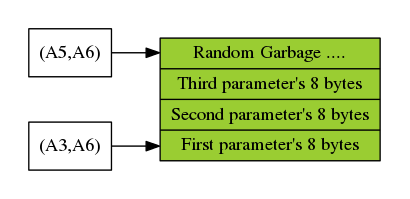
\includegraphics[width=0.5\textwidth]{Content/images/Name_Table_Entries.png}
\caption{Name Table Entries for Three Parameters.}
\label{fig:NameTableEntriesForThreeParameters}
\end{figure}

So (A3,A6) points to the first byte of the first parameter and is
    the lowest address, (A5,A6) points to the first byte past the last
    parameter and is the highest address.

The first name table entry starts at 0(A3,A6) and ends at 7(A3,A6).
    The second starts at 8(A3,A6) and ends at 15(A3,A6) and the last starts at
    16(A3,A6) and stops at 23(A3,A6).

When fetching parameters from the name list onto the maths stack, we
    can use some vectored utilities to get them for us. These allow the
    retrieval of strings, long words, integers (short words) and floating
    point values. They all expect A3 and A5 to be set up correctly as above.
    A3 and A5 are trashed by the routines, so if you have to check any
    parameter separators etc, then you must do it before calling the fetch
    routines.

When the routines return, they set D3.W to the number of parameters
    fetched and set A1 to the correct value for the top of the maths stack -{}
    relative to A6 of course. Now we can access the values of each parameter
    separately as we like. On return the first parameter in the list is stored
    at 0(A1,A6), the next is above the first and so on. When fetching
    parameters p1, p2, p3 from a procedure or function call, they will end up
    on the maths stack in the correct order -{} 0(A1,A6) will be pointing at p1
    on the stack.

The parameter fetching routines are listed in Table~\ref{tab:VectoredRoutinesForParameterFetching}.
\begin{table}[htbp]
\centering
\begin{tabular}{l l}  % Set this correctly ...
\toprule
\textbf{Vector} & \textbf{Purpose} \\
\midrule
%
\vector{CA\_GTINT} & fetch integer parameters (2 bytes each).\\
\vector{CA\_GTLIN} & fetch long parameters (4 bytes each).\\
\vector{CA\_GTFP} & fetch floating point parameters (6 bytes each).\\
\vector{CA\_GTSTR} & fetch string parameters (variable length).\\
%
\bottomrule
\end{tabular}
\caption{Vectored Routines For Parameter Fetching.}
\label{tab:VectoredRoutinesForParameterFetching}
\end{table}


They require to be called as follows:

\begin{lstlisting}[firstnumber=1,caption={Using the Vectored Parameter Fetching Utilities},label={lst:ParameterFetchingUtilities}]
start   move.w  ca_gtint,a2     ; Fetch all params as word ints
        jsr     (a2)            ; Do it
        tst.l   d0              ; Did it work?
        beq.s   ok              ; Yes
        rts                     ; Return to SuperBasic

ok      ...                     ; carry on here
\end{lstlisting}

At this point, D3.W can be tested to check that the correct number
    of parameters has been fetched.

\begin{lstlisting}[firstnumber=1,caption={Checking Parameter Counts},label={lst:CheckingParameterCounts}]
start   cmpi.w  #4,d3           ; Were there 4 parameters?
        beq.s   ok_4            ; Yes
        moveq   #-15,d0         ; Bad parameter error code = -15
        rts                     ; and back to SuperBasic

ok_4    ...                     ; Carry on here
\end{lstlisting}

To access the parameters we need to get the data off of the maths
    stack and into our working registers, as follows:

\begin{lstlisting}[firstnumber=1,caption={Fetching Parameter Values},label={lst:FetchingParameterValues}]
        move.w  0(a6,a1.l),d1   ; Parameter one
        move.w  2(a6,a1.l),d2   ; Parameter two
        move.w  4(a6,a1.l),d3   ; Parameter three
        move.w  6(a6,a1.l),d4   ; Parameter four
\end{lstlisting}

and so on. Now that we have our parameters, we need do nothing more
    with the maths stack if we are inside the code of a procedure. If we are
    in a function then we \emph{must} tidy the maths stack. This is simply done by
    adding the size of all parameters on the stack to A1. In our example we
    have 4 word length parameters, so we should add 8 to A1 as follows
   :

\begin{lstlisting}[firstnumber=1,]
        adda.l  #8,a1           ; Reset maths stack
\end{lstlisting}

As mentioned, there is no need to do this in a procedure, but if you
    have to learn to do it for a function, you are as well to learn to do it
    for everything -{} that way you don't forget to do it and cause a hanging
    QL.

Tidying a stack with strings on is more difficult and it is probably
    best done as each one is removed. For example, say we have two strings on
    the stack after a call to \vector{CA\_GTSTR} then we get them off as follows
   :
\index{Tidying the Maths Stack}
\begin{lstlisting}[firstnumber=1,caption={Tidying a String from the Maths Stack - Part 1},label={lst:StringStackTidyPart1}]
    cmpi.w  #2,d3           ; Were there two strings?
    beq.s   ok              ; Yes
    moveq   #-15,d0         ; Bad parameter
    rts                     ; Exit to SuperBasic

ok  lea     buffer_a,a2     ; Destination for one string
    lea     0(a6,a1.l),a3   ; Source for string
    bsr     copy_str        ; Copy
    move.w  0(a6,a1.l),d0   ; Size word
    addq.w  #3,d0           ; Make bigger
    bclr    #0,d0           ; Make even
    add.w   d0,a1           ; This will sign extend remember!
\end{lstlisting}

Ok, so we added the size of the first string plus 2 for the size of
    the size word as well, to A1 having made it even so the stack is now
    cleared of the first string. This leaves one string with its size word
    sitting at 0(A6,a1.l) ready for the next copy:

\begin{lstlisting}[firstnumber=1,caption={Tidying a String from the Maths Stack - Part 2},label={lst:StringStackTidyParty2}]
    lea     buffer_b,a2     ; Destination for next string
    lea     0(a6,a1.l),a3   ; Source for string
    bsr     copy_str        ; Do the copy
    move.w  0(a6,a1.l),d0   ; Size word
    addq.w  #3,d0           ; Make bigger
    bclr    #0,d0           ; Make even
    add.w   d0,a1           ; This will sign extend too!
\end{lstlisting}

and there you have a tidy stack once again.

You could ask `if we have to restore A1 to its value on entry, why
    not just save A1 and then restore it afterward?'. Like this:

\begin{lstlisting}[firstnumber=1,caption={How to Hang the QL},label={lst:HowToHangTheQL}]
start   move.l  bv_rip(a6),a1   ; Fetch top of Maths Stack
        move.l  a1,-(a7)        ; Stack it for later

        ; Do lots of stuff here - fetching parameters etc

        move.l  (a7)+,a1        ; Restore A1

        ; and so on
\end{lstlisting}

Well, you could, but at certain times there will be a hung QL and
    you will not know why. The reason is simple, but difficult to find or
    trace. When you fetch parameters onto the maths stack, it can \emph{move around in memory}. Preserving the original value is fine if the stack stays put, but
    if it moves and you set BV\_RIP to the old value, you can get into all
    sorts of trouble. It is best to keep the stack tidy using the methods
    described above.

\subsection{Keeping Things Even}
\label{ch7-keep-things-even}%\hyperlabel{ch7-keep-things-even}%

You may well also ask ``What is all this add 3 and clear bit 0
      nonsense then?'' Think about it in binary for a bit. We have the word
      size of the string in D0.W and we must ensure that we add an even number
      of bytes to A1. We must also remember to add 2 to A1 for the size of the
      size word itself.

Lets try this with an even number first of all. Even numbers are
      detected by bit zero being clear, so:
\begin{table}[htbp]
\centering
\begin{tabular}{c c c}  % Set this correctly ...
\toprule
\textbf{D0} & \textbf{D0 + 3} & \textbf{Result} \\
\midrule
%
2 & 5 & 4\\
4 & 7 & 6\\
10 & 13 & 12\\
%
\bottomrule
\end{tabular}
\caption{Keeping even numbers even.}
\label{tab:KeepingEvenNumbersEven}
\end{table}

So you can see what is happening. D0 always ends up being D0 + 2
      and is always even. This is good as it is what we want. What about odd
      numbers then?

\begin{table}[htbp]
\centering
\begin{tabular}{c c c}  % Set this correctly ...
\toprule
\textbf{D0} & \textbf{D0 + 3} & \textbf{Result} \\
\midrule
%
3 & 6 & 6\\
5 & 8 & 8\\
11 & 14 & 14\\
%
\bottomrule
\end{tabular}
\caption{Keeping odd numbers even.}
\label{tab:KeepingOddNumbersEven}
\end{table}


So is this good then? Remember that the maths stack must be kept
      even. When odd length strings are copied onto it by \vector{CA\_GTSTR} it pads out
      the space on the stack with a rubbish byte (CHR\$(0) to be precise) which
      is never used. The size word remains odd.

So for an odd sized string we need to add 2 for the size word, the
      odd number of bytes and one spare for the padding. Our 3 lines of code
      handle this for all cases -{} even or odd sized strings. The code is good!

Of course it would be simple to do this:

\begin{lstlisting}[firstnumber=1,caption={Long Way to Keep Things Even},label={lst:LonegWayToKeepThingsEven}]
        move.w  0(a6,a1.l),d0   ; Size word
        btst    #0,d0           ; Is it even?
        beq.s   even            ; Yes
        addq.w  #1,d0           ; Add 1 for padding byte

even    addq.w  #2,d0           ; Add 2 ro the size word
        add.w   d0,a1           ; And add with sign extension
\end{lstlisting}

But this is extra typing and takes longer, so the simple case
      shown above, works all the time.

\subsection{Two Of These And One Of Those Please}\index{Fetching mixed type parameters}
\label{ch7-mixed-parameters}%\hyperlabel{ch7-mixed-parameters}%

What do you do if you want to get hold of two long words and a
      string?

Let us assume that you are writing an extension procedure that has this
      format:

\begin{lstlisting}[firstnumber=1,]
DO_SOMETHING long_1, long_2, string_1
\end{lstlisting}

This has two different types of parameters and we cannot fetch
      them all in one go unless we can read the long parameters as strings and
      convert them ourselves. It is quite easy to fetch these parameters -{} you
      just do it in two goes.

In the code we know that A3 and A5 hold the start and stop
      addresses of the parameters in the Name Table. If we set A5 to be A3 +
      16 and then collect long words we will get our two long words. We can
      then set A5 back to its original value and set A3 to this less 8 and
      fetch the final parameter as a string. Here we go then:

\begin{lstlisting}[firstnumber=1,caption={Fetching Mixed Type Parameters},label={lst:FetchingMixedTypeParameters}]
get_longs   move.l  a5,-(a7)        ; Save last parameter pointer
            lea     16(a3),a5       ; Set A5 for two parameters
            move.w  ca_gtlint,a2    ; Fetch all (2) longs
            jsr     (a2)            ; Do it
            tst.l   d0              ; OK?
            beq.s   got_long        ; Yes
            rts                     ; Exit with error code

got_long    cmpi.w  #2,d3           ; Were there two?
            bne.s   bad_params      ; No, bale out
            move.l  (a7)+,a5        ; A5 holds address of p3
            lea     -8(a5),a3       ; There can be only one!
            move.w  ca_gtstr,a2     ; Fetch as strings now
            jsr     (a2)            ; Do it
            tst.l   d0              ; OK?
            beq.s   got_string      ; Yes
            rts                     ; Exit with error code

bad_params  moveq   #-15,d0         ; Bad parameter error
            rts                     ; Exit to SuperBasic

got_string  ; continue from here
\end{lstlisting}

Ok, so now what does the maths stack look like? Remember when
      fetching parameters they end up on the stack in the order you want them
      with the first at the lowest address and the next above it and so on.
      This time, we fetched two longs and a string in two different calls.
      This means that after the first fetch the maths stack looks like  	    \figurename~\ref{fig:MathsStackAfterTwoLongInts}:

\begin{figure}[h]
\center
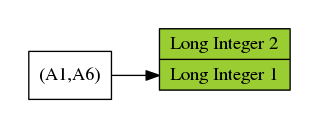
\includegraphics[width=0.5\textwidth]{Content/images/Maths_Stack_2_Long.png}
\caption{Maths Stack After Fetching Two Long Integer Parameters.}
\label{fig:MathsStackAfterTwoLongInts}
\end{figure}

But then we fetched a string and it got put onto the maths stack
      so it now looks like \figurename~\ref{fig:MathsStackAfterTwoLongIntsPlusString}:

\begin{figure}[h]
\center
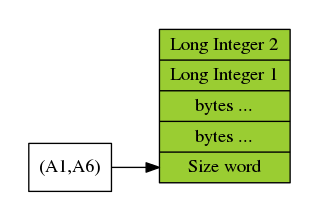
\includegraphics[width=0.5\textwidth]{Content/images/Maths_Stack_2_Long_and_String.png}
\caption{Previous Maths Stack After Fetching a String Parameter.}
\label{fig:MathsStackAfterTwoLongIntsPlusString}
\end{figure}

QDOS is very helpful here. If during the course of fetching the
      string, the maths stack had to be moved in memory, QDOS will preserve
      the current contents so that `long\_1' and `long\_2' will still be there
      when you come around to using their values. Nice!

In this discussion we mentioned the name table. This is discussed
      in detail next. Do you get the feeling that this chapter is written upside down?

\section{Name Table Entries}\index{Name Table}
\label{ch7-name-table}%\hyperlabel{ch7-name-table}%

The name table is a list of 8 byte entries which define all the
    names used in SuperBasic (or extensions to SuperBasic written in
    assembler), the type of each entry and where it lives in the name list and
    the SuperBasic variables area.

As per the description above (GETTING PARAMETERS), the name table is
    also used to store details of the parameters passed to our assembly
    routine. So for parameters passed, a copy is made and stored at the end of
    the name table. The A3 and A5 registers are set up to point at the first
    and last parameter and for these, the format of the name table is as
    follows:
\begin{table}[htbp]
\centering
%\begin{tabular}{l l l}  % Set this correctly ...
%\begin{tabular}{p{0.2\linewidth}p{0.5\linewidth}p{0.2\linewidth}}
%\begin{tabular}{p{0.2\textwidth}p{0.5\textwidth}p{0.2\textwidth}}
\begin{tabular}{p{0.2\columnwidth}p{0.4\columnwidth}p{0.3\columnwidth}}\toprule
\textbf{Bytes 0 \& 1} & \textbf{Bytes 2 \& 3} & \textbf{Bytes 4 to 7} \\
\midrule
%
Type \& separator flag word. &
Pointer to a NAME LIST entry which \emph{may} be an odd address. &
Pointer to value in the variables area. \\
%
\bottomrule
\end{tabular}
\caption{Parameter format on the name table.}
\label{tab:NameTableParameterFormat}
\end{table}

The low byte of the type word tells us what type of parameter we are
    dealing with and its separator(s) as shown in Table~\ref{tab:ParameterTypesAndSeparators}.

\begin{table}[htbp]
\centering
\begin{tabular}{l l}  % Set this correctly ...
\toprule
\textbf{Bytes 0 \& 1} & \textbf{Bytes 2 \& 3} \\
\midrule
%
Bit 7 & 0 = There is not a hash (\#) in front of this parameter\\
Bit 7 & 1 = There is a hash (\#) in front of this parameter\\
Bits 6 -{} 4 & 000 = No separator after this parameter\\
Bits 6 -{} 4 & 001 = Comma (,) after this parameter\\
Bits 6 -{} 4 & 010 = Semi-{}colon (;) after this parameter\\
Bits 6 -{} 4 & 011 = Back-{}slash (\textbackslash{}) after this parameter\\
Bits 6 -{} 4 & 100 = Exclamation mark (!) after this parameter\\
Bits 6 -{} 4 & 101 = TO after this parameter\\
Bits 3 -{} 0 & 0000 = Null\\
Bits 3 -{} 0 & 0001 = String\\
Bits 3 -{} 0 & 0010 = Floating point\\
Bits 3 -{} 0 & 0011 = Integer\\
%
\bottomrule
\end{tabular}
\caption{Parameter types and separators.}
\label{tab:ParameterTypesAndSeparators}
\end{table}

For the first parameter, the type byte is at 1(a6,a3.l) as opposed
    to 0(a6,a3.l).

For the rest of SuperBasic, the name table uses bytes 0 and 1 to
    define the type of the entry as shown in  Table~\ref{tab:SuperBasicParameterDetailsByte0And1}.

\begin{table}[htbp]
\centering
\begin{tabular}{l l}  % Set this correctly ...
\toprule
\textbf{Byte 0 Value} & \textbf{Description} \\
\midrule
%
\$00 & Undefined\\
\$01 & Expression\\
\$02 & Variable\\
\$03 & Array or substring\\
\$04 & SuperBasic PROCedure (Byte 1 is always zero)\\
\$05 & SuperBasic FuNction\\
%
\bottomrule
\end{tabular}
\caption{SuperBasic specific parameter details -{} byte 0.}
\label{tab:SuperBasicParameterDetailsByte0}
\end{table}

\begin{table}[htbp]
\centering
\begin{tabular}{l l}  % Set this correctly ...
\toprule
\textbf{Byte 1 Value} & \textbf{Description} \\
\midrule
%
\$00 & Substring (Internal use only!)\\
\$01 & String\\
\$02 & Floating point.\\
\$03 & Integer\\
%
\bottomrule
\end{tabular}
\caption{SuperBasic specific parameter details -{} byte 1.}
\label{tab:SuperBasicParameterDetailsByte1}
\end{table}

\begin{table}[htbp]
\centering
\begin{tabular}{l l}  % Set this correctly ...
\toprule
\textbf{Bytes 0 \& 1 Value} & \textbf{Description} \\
\midrule
%
\$0602 & REPeat loop identifier\\
\$0702 & FOR loop identifier\\
\$0800 & Assembly language procedure\\
\$0900 & Assembly language function\\
%
\bottomrule
\end{tabular}
\caption{SuperBasic specific parameter details -{} bytes 0 and 1 together.}
\label{tab:SuperBasicParameterDetailsByte0And1}
\end{table}


\begin{note}
The REPeat and FOR loop identifiers are hard coded to be of type
      floating point. This represents the internal values for SuperBasic. I
      suspect that this is the reason that FOR loop identifiers cannot be
      integer. 

SBASIC, on the other hand, under SMSQ allows integer FOR loops and I presume
      that the internal format for these will be \$0703 -{} I am sure that Jochen
      will correct me if I am wrong!!
\end{note}

For all entries in the name table, be they parameters or `proper'
    names, have a word in bytes 2 \& 3 which points to the entry in the
    name list for this `name'. This simply gives an easy way of storing the
    names all in one place. Note that this value is simply the offset from the
    start of the name table where the bytes of this name can be found. A
    fuller description of the name list follows on below.

If the value is -{}1, then this is an expression and has no
    name.

Finally, there is a long word which is the pointer to the variables
    area. If this value is negative then the variable is undefined and has no
    entry there. Again, this value is an offset into the variables area and
    not an absolute address.

\section{Name List}\index{Name List}
\label{ch7-name-list}%\hyperlabel{ch7-name-list}%

The name list is a simple structure in SuperBasic. It holds the
    names of all procedures, variables, functions etc that have ever been used
    in this session at the QL. It is odd in that each name is preceded by a
    \emph{byte} defining its length as opposed to a word in the normal QDOS manner.
    This implies that names can be up to 255 characters long. There are no
    padding bytes to force even addresses in the name list either. Beware when
    accessing this area that you only do byte sized operations!

The name list starts at the address BV\_NLBAS(A6) to BV\_NLP(A6) with
    BV\_NLBAS(A6) being the lowest address and BV\_NLP(A6) pointing to the first
    byte \emph{after} the last entry in the name list. As usual, the offsets you get
    from these basic variables are themselves relative to A6!

To explain further, Fetch the offsets from BV\_NLBAS(A6) into A0. The
    address 0(A6,A0.L) is the start of the name list. Or, in code:

\begin{lstlisting}[firstnumber=1,]
start   move.l  BV_NLBAS(a6),a0
        lea.l   0(a6,a0.l),a0
        move.b  0(a0),d0         ; D0 = size of the first entry
        ...                      ; More code here
\end{lstlisting}

Now A0 has the start of the name list, but beware of doing this in
    case SuperBasic gets moved. It is best to stay relative as in the
    following:

\begin{lstlisting}[firstnumber=1,]
start   move.l  BV_NLBAS(a6),a0
        move.b  0(a6,a0.l),d0    ; D0 = size of the first entry
        ...                      ; More code here
\end{lstlisting}

This is much safer.

The internal structure therefore looks like \figurename~\ref{fig:SuperBasicNameListStructure}.

\begin{figure}[h]
\center
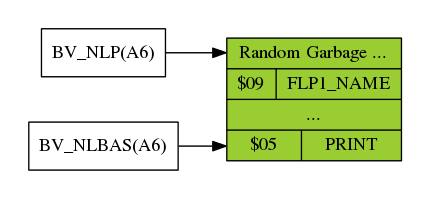
\includegraphics[width=0.5\textwidth]{Content/images/Name_List.png}
\caption{SuperBasic Name List Structure.}
\label{fig:SuperBasicNameListStructure}
\end{figure}

How is the name list useful to us in writing procedures and
    functions? consider these commands:

\begin{lstlisting}[firstnumber=1,]
OPEN_IN #3,'ram1_test_file'
OPEN_IN #3,ram1_test_file
\end{lstlisting}

What is the difference? In the first case, the parameter for the
    filename is a quoted string and internally, the OPEN\_IN routine can fetch
    it using \vector{CA\_GTSTR} as described above. In the second, it will fail if it
    uses \vector{CA\_GTSTR} because without quotes, the parameter is a NAME and not a
    STRING.

The procedure/function writer must check for a string parameter or a
    name parameter and treat each accordingly. How is this done? -{} use the
    name table type byte as described above.

In the procedure or function, process a name as follows:

Assuming that A3 points to the name table entry for this parameter,
    then if bits 0 to 4 of 1(a6,a3.l) is zero then we have a name and not a
    variable. We must copy the bytes of name, from the entry in the name list, to the stack (or to the appropriate buffer) making sure that the size byte in the name list is converted to a
    size word on the stack or in the buffer. The following fragment of code
    gives the general idea:

\begin{lstlisting}[firstnumber=1,]
name_test   move.b  1(a6,a3.l),d0
            andi.b  #$0f,d0
            bne.s   not_name
got_name    ;
            ; Must be a name so process accordingly here
            ;
not_name    ; Process a string here
\end{lstlisting}

So when a name is detected we have to make space for it, copy the
    size \emph{byte} from from the name list into the size \emph{word} in our string buffer
    (which has to be word aligned on an even address) and then copy the
    individual bytes from the name list to the string buffer. At this point we
    are in the same situation we would be in had we fetched a string using
    \vector{CA\_GTSTR} and copied it from the maths stack into our buffer. Simple? (In
    my famous DJToolkit\program{DJToolkit} extensions I never actually bothered doing this and I
    simply fetched all filenames etc as strings -{} if the user supplied a name
    instead, the procedure or function complained. So far no-{}one has
    requested that it be updated to allow names!)

\program{NLIST}\index{Printing the Name List}How about a bit of fun -{} lets write a procedure that prints the
    entire name list to a channel. It shall be called nlist and it shall take
    one parameter which is the channel number -{} this will default to \#1 if no
    parameter supplied.

\begin{lstlisting}[firstnumber=1,caption={Procedure to Print the Entire Name List},label={lst:NlistProcedure}]
bv_nlbas    equ     $20             ; Base of name list
bv_nlp      equ     $24             ; End of name list
bv_chbas    equ     $30             ; Base of channel table
bv_chp      equ     $34             ; End of channel table
err_no      equ     -6              ; Channel not open error
err_bp      equ     -15             ; Bad parameter error

start       lea     define,a1       ; Pointer to the definitions
            move.w  BP_INIT,a2      ; The vector we need to use
            jsr     (a2)            ; Call the vectored routine
            rts                     ; Return to SuperBasic

*----------------------------------------------------------------
* Definition table for one new procedure
*----------------------------------------------------------------
define      dc.w    1               ; 1 new procedure
            dc.w    nlist-*         ; Offset to procedure
            dc.b    5,'NLIST'       ; Size and name
            dc.w    0               ; End of procedures

            dc.w    0               ; Number of functions
            dc.w    0               ; End of functions

*----------------------------------------------------------------
* Procedure NLIST starts here ...
*
* Check for one or zero parameters - if not then error exit
*----------------------------------------------------------------
nlist       cmpa.l  a3,a5           ; No parameters?
            beq.s   nl_none         ; Yes, skip
            move.l  a5,d0           ; Last parameter pointer
            sub.l   a3,d0           ; minus first
            cmpi.w  #8,d0           ; One parameter?
            beq.s   got_one         ; Yes

bad_par     moveq   #-15,d0
error_exit  rts

*----------------------------------------------------------------
* If one parameter, must have a hash else error exit
*----------------------------------------------------------------
got_one     btst    #7,1(a6,a3.l)   ; check for a hash
            beq.s   bad_par         ; Not got one

*----------------------------------------------------------------
* It has a hash - fetch the channel id. If this fails, error exit.
*----------------------------------------------------------------
get_one     move.w  ca_gtint,a2     ; Vector for word integers
            jsr     (a2)            ; Fetch!
            tst.l   d0              ; Ok?
            bne.s   error_exit      ; No, bale out
            cmpi.w  #1,d3           ; One only?
            bne.s   error_exit      ; No, bale out
            move.w  0(a6,a1.l),d0   ; Fetch channel number
            addq.l  #2,a1           ; Tidy stack
            tst.w   d0              ; Set flags
            blt.s   bad_par         ; Negative is a bad id
            bra.s   chan_ok         ; skip default handling

*----------------------------------------------------------------
* No parameters supplied - default channel number to #1
*----------------------------------------------------------------
nl_none     moveq   #1,d0           ; Default to channel #1
chan_ok     bsr.s   channel_id      ; convert to channel id in A0
            bne.s   error_exit      ; Oops!

*----------------------------------------------------------------
* Fetch the start of the name list from BV_NLBAS(A6). The result 
* of this is an offset from A6 to where the namelist actually 
* starts.
*----------------------------------------------------------------
            move.l  bv_nlbas(a6),a3 ; Start of name list 
*                                   ; Relative to A6!

*----------------------------------------------------------------
* Our main loop starts here. We test to see if we are finished 
* and if not copy the (next) name to the buffer formatting it as 
* a QDOS string. 
* D3 is preserved inside the loop, so set it once just before the 
* loop starts.
*----------------------------------------------------------------
            moveq   #-1,d3          ; Timeout for the channel

nl_loop     cmpa.l  bv_nlp(a6),a3   ; Compare offsets - done?
            bge.s   nl_done         ; Yes
            moveq   #io_sstrg,d0    ; Print some bytes please
            move.b  0(a6,a3.l),d2   ; Counter byte from name list
            ext.w   d2              ; Needs to be word sized
            lea     1(a6,a3.l),a1   ; Start of bytes to print
            adda.w  d2,a3           ; Adjust to end of bytes
            addq.l  #1,a3           ; A3 = next entry, size byte
            trap    #3              ; Print the name 
*                                   ; Preserves A0, A3 and D3
            tst.l   d0              ; Ok?
            bne.s   error_exit      ; Oops - failed

nl_nl       moveq   #io_sbyte,d0    ; Code for 'send one byte'
            moveq   #10,d1          ; Newline character
            trap    #3              ; Print newline
*                                   ; Preserves A0, A3 and D3
            tst.l   d0              ; Ok?
            bne.s   error_exit      ; Oops - failed

            bra.s   nl_loop         ; Lets go round again!

*----------------------------------------------------------------
* If there is no more to do, return to SuperBasic.
*----------------------------------------------------------------
nl_done     moveq   #0,d0           ; No errors
            rts                     ; Exit to SuperBasic

*----------------------------------------------------------------
* Copy the above code for the CHANNEL_ID subroutine to here as it
* is required.
*----------------------------------------------------------------
channel_id ...
\end{lstlisting}

Save the file, assemble, fix typing errors and test -{} super stuff
    this eh?

When this procedure runs, you can see all the internal names like
    PRINT, CLOSE etc and also all your own stuff like NLIST, GREEN, RED etc
    and also any filenames that you have used without quotes around them.
    These are names like anything else.

if you try the following:

\begin{lstlisting}[firstnumber=1,]
open_new #3,ram1_test
nlist #3
close #3
\end{lstlisting}

then load ram1\_test into your editor (or copy to scr\_), the last
    entry in the name list will be ram1\_test -{} because you didn't use quotes.
    If you now try:

\begin{lstlisting}[firstnumber=1,]
open_new #3,"ram1_test_again"
nlist #3
close #3
\end{lstlisting}

This time, ram1\_test\_again will NOT be in the list because it is not
    a name, simply a string. This routine can be used to get a list of all
    procedures, functions, names etc that are loaded into your QL.

\section{The Maths Stack}\index{Maths Stack}
\label{ch7-maths-stack}%\hyperlabel{ch7-maths-stack}%

The maths stack is where all internal mathematical calculations of
    floating point variables are done. It is also used to allow parameters
    passed to machine code procedures and functions to be `collected' from the
    user and passed to the registers etc for use by the procedure or
    function.

The maths stack is simply an area of memory which can be used for
    all these fancy calculations, parameter handling etc. There is nothing
    (much) special about it and it is \emph{always} addressed internally using
    register A1 (relative to A6 -{} but you knew that didn't you?)

One of the first things I learned when writing extensions to
    SuperBasic was that on entry to a function or procedure, the A1 register
    is set to a value corresponding to the top of the maths stack. This is a
    \emph{myth} and is not correct.

The value in register A1 can be anything on entry to a machine code
    function or procedure. I have done a lot of investigating (thanks to
    QMON2\program{QMON2}) and come up with the following rule:

If you want a suitable value in A1 for the top of the maths stack,
    then either fetch some parameters, or, load it from BV\_RIP.

This means that if a function wants to return a value -{} which
    functions usually do -{} and the function has no parameters then you must
    load A1 from BV\_RIP(A6) before calling the \vector{BV\_CHRIX} vector to reserve
    space. As I found out to my cost, not setting A1 is a good way to trash
    the system!

If your function does have parameters, then AFTER they have been
    fetched, A1 is set ok, up until that time, it is not and has the following
    possible values:

\subsection{A1 Is Negative}
\label{ch7-A1-negative}%\hyperlabel{ch7-A1-negative}%

If A1 is a negative number, then your function has been called as
      part of an expression such as:

\begin{lstlisting}[firstnumber=1,]
PRINT 10 * MY_FUNCTION(p1, p2, p3 ....)
\end{lstlisting}

The number in A1.L is the number of bytes that have already been
      used on the maths stack for the `10' in this case. This will be -{}6 as
      the 10 will be stored as a floating point number.

\subsection{A1 Is Zero}
\label{ch7-A1-zero}%\hyperlabel{ch7-A1-zero}%

If the number in A1 is zero, then your function has been called
      thus:

\begin{lstlisting}[firstnumber=1,]
PRINT MY_FUNCTION(p1, p2, p3 ....)
\end{lstlisting}

or

\begin{lstlisting}[firstnumber=1,]
PRINT MY_FUNCTION(p1, p2, p3 ....) + 10
\end{lstlisting}

and no bytes have been used on the maths stack yet.

\subsection{A1 Is Positive}
\label{ch7-A1-positive}%\hyperlabel{ch7-A1-positive}%

If A1.L is greater than zero then this implies that there are A1.L
      many bytes available on the maths stack and calling \vector{BV\_CHRIX} to allocate
      stack space will not move the maths stack around in memory.

\begin{warning}
I have \emph{never} seen this documented and it
        has been discovered by me during long debugging sessions. Now that
        SMSQ is here, the above information may no longer be valid. The
 \emph{only} thing to remember is that on entry to a
        procedure or function, A1 \emph{does not} hold a
        suitable value for the top of the maths stack as stated in various
        documents.
\end{warning}

So that is the real situation and not as specified in the
      documentation. I took ages to debug one simple function I wrote, which
      had no parameters and required some space on the maths stack for its
      result. Take a look at the code in the colour functions (green, red etc)
      we wrote back at the start of this article and you will see the
      following code:

\begin{lstlisting}[firstnumber=1,]
return_d7   move.l  bv_rip(a6),a1   ; Because we had no params
            moveq   #2,d1           ; Size of stack space needed
            move.w  bv_chrix,a2     ; Allocate maths stack space
            jsr     (a2)            ; Get some space
\end{lstlisting}

As you can now see, we load A1 from BV\_RIP because none of the
      functions had any parameters passed. Had that one line of code been
      missed out, your QL would have crashed. Try it if you like!

Values on the maths stack must be stored at even addresses. For
      integers, long integers and floating point values, this is not a
      problem. Strings, on the other hand, must be set up correctly with the
      word defining the size n an even address and the bytes of the string
      following. Odd length strings should have an extra padding byte to keep
      the A1 maths stack pointer even.

If you read back to section ~\ref{ch7-keep-things-even} `Keeping things
      even' then you will see how to do this. If you are returning a string
      from a function, you will need to reserve space for the string, its
      word count and a possible spare byte for padding. Refer to the
      explanation above and you will see why the following code `just works'
     :

\begin{lstlisting}[firstnumber=1,]
ret_string  move.w  (a0),d1         ; Assume string is at (A0)
            addq.w  #3,d1           ; Add size word + padding
            bclr    #0,d1           ; Force even size
            move.w  bv_chrix,a2     ; Allocate maths stack space
            jsr     (a2)
\end{lstlisting}

Of course, I am assuming that A1 holds a suitable value. The code
      above will request an even amount of space for a string result. First we
      fetch the length into D1 -{} this is the number of characters in the
      string only.

We then add 3 to D1. This is 2 for the word count and one for a
      possible padding byte. By clearing bit zero of D1 we force the number to
      be even and can then carry on with the request for space etc. Easy stuff
      this!

\section{Returning Values From Functions}\index{Function Return Values}
\label{ch7-returning-values}%\hyperlabel{ch7-returning-values}%

When returning values on the maths stack you must be very careful.
    When a function exits there must be a value on the top of the maths stack
    the pointer to this value needs to be stored in BV\_RIP(A6) and D4 has to
    have a values in it which defines the returned parameter type. See Table ~\ref{tab:FunctionReturnDataTypes}.

\begin{table}[htbp]
\centering
\begin{tabular}{l l}  % Set this correctly ...
\toprule
\textbf{D4} & \textbf{Return Parameter Type} \\
\midrule
%
1 & String\\
2 & Floating point\\
3 & Word integer\\%
\bottomrule
\end{tabular}
\caption{Function Return Data Types}
\label{tab:FunctionReturnDataTypes}
\end{table}

Notice anything missing? Although we are allowed to fetch long
    integers as parameters, we are not allowed to return them. This is a
    problem and the usual fix is to convert a long integer to a floating point
    and return that instead. This will be covered in another thrilling episode
   !

\section{Channel Tables}\index{SuperBasic Channel Table}
\label{ch7-channel-table}%\hyperlabel{ch7-channel-table}%

In our procedure PSI\_CLS\program{PSI\_CLS}, we use a channel number in SuperBasic. In
    assembler, this is no use to us as all internal operations that require a
    channel (CLS, PAPER etc) require a channel id which is a 32 bit long
    number which bears no resemblance (or only coincidentally) to a SuperBasic
    channel number.

In QDOS there is a channel table -{} for the entire system, and there
    is the SuperBasic channel table which is used to convert channel numbers
    into channel ids which is what we require. SuperBasic keeps us away from
    nasty things like internal representations -{} assembler does not.

The routine we used above, channel\_id, is all that is required to
    convert a channel number to a channel id. It looks at the SuperBasic
    channel table and for each channel that has been opened (even if it is now
    closed) there will be an entry in the channel table. Each entry is \$28
    bytes long (40 bytes) and has the structure shown in Table ~\ref{tab:SuperBasicChannelTableDefinition}.

\begin{table}[htbp]
\centering
\begin{tabular}{l l p{0.75\linewidth}}  % Set this correctly ...
\toprule
\textbf{Offset} & \textbf{Size} & \textbf{Purpose} \\
\midrule
%
\$00 & Long    & QDOS internal channel id\\
\$04 & 6 bytes & Graphics cursor X position (Floating Point format)\\
\$0A & 6 bytes & Graphics cursor Y position (Floating Point format)\\
\$10 & 6 bytes & Turtle angle (Floating Point format)\\
\$16 & Byte    & Pen status (0 = up or 1 = down)\\
\$20 & Word    & Character position on line for PRINT and INPUT etc\\
\$22 & Word    & Width of the channel. Set by WIDTH command in SuperBasic but defaults to 80 when OPEN is called.\\
\$24 & Long    & Spare -{} currently unused\\
%
\bottomrule
\end{tabular}
\caption{SuperBasic Channel Table Definition}
\label{tab:SuperBasicChannelTableDefinition}
\end{table}


When a channel is opened in SuperBasic, an entry is created (or
    reused) in this table. At startup channels \#0, \#1, and \#2 are pre-{}created
    and that is all. If you now open \#4, a new entry will be created for it.
    If you open channel \#10, then blank entries are created for all the
    `in-{}between' channels (5 to 9) and entry 10 is then created and
    initialised on top.

A channel that has never been opened can therefore still have an
    entry in this table -{} channels 5 to 9 in the above example. All of these
    use memory so it is advisable to start with 3 and work upwards opening
    channels as you go, rather than opening \#100 or something similar which
    needlessly wastes 40 bytes of memory for each unused channel.

A channel that is closed, or has never been opened, has a QDOS
    channel id which is negative.

In the Basic variables area in QDOS (to be covered in a later issue
    -{} and by the way, I refer to the variables that hold information about
    SuperBasic, and not variables you create in SuperBasic!) BV\_CHBAS holds
    the offset from A6 to the first entry in the table (ie channel \#0) and
    BV\_CHP holds the offset from A6 to the first byte after the last entry in
    the channel table. Don't forget that these are offsets and that everything
    in SuperBasic is relative to A6 -{} simply because by doing this the base
    address for the job (SuperBasic is just another job in the machine) is
    held in A6. If everything else is stored as an offset then moving the job
    in memory is simple as only the A6 register has to be updated.

Take a look at the code for channel\_id again and note how we are
    using addresses that are relative to A6. Make sure that you understand
    because all fiddling in the bowels of SuperBasic requires that you
    understand relative addressing.

Most of the time you will only be interested in the conversion from
    SuperBasic channel number to QDOS channel id.

\section{Exercise}
\label{ch7-exercise}%\hyperlabel{ch7-exercise}%

As an exercise, why not add a new procedure called \program{PSI}PSI to the code
    for PSI\_CLS.\program{PSI\_CLS} This new procedure will carry out all the same work as
    PSI\_CLS but it will not do the CLS part of it. This will be useful when
    you want to set the colours for a window but not clear it. I will NOT be
    giving the answers out next time, but here are a few hints:
\begin{itemize}[itemsep=0pt]

\item{}update the definition table with details of the new
        procedure.


\item{}in the proc's code, set D6.B to zero for PSI and 1 for PSI\_CLS.
        Do this as the first instruction in both procedures.


\item{}In the PSI procedure, simply set D6 and jump to the code in
        PSI\_CLS.


\item{}Just before doing the actual CLS part of PSI\_CLS, check the
        value in D6.B and if zero, don't do the CLS simply BRA.S to error\_exit
        instead.

\end{itemize}

All in all, I think this can be done in about 10 extra lines of
    code, maybe less, not counting the extra lines in the definition
    block.

\begin{warning}
Adding even a few lines of code can sometimes cause any `short'
      branches to go out of range and this will cause errors in the assembly.
      If this happens, simply find the ones in error and remove the `.s' from
      the `bsr' or `bra' instructions.
\end{warning}

\section{Coming Up...}
\label{ch7-the-end}%\hyperlabel{ch7-the-end}%

In the next chapter we delve into the QL's screen layout and using
    our new found knowlege of assembly language programming, we will develop a
    mode 4 `plot' routine in assembler. If you find this easy, there is an
    exercise for the reader -{} to develop the corresponding mode 8 `plot' code
   !



\chapterimage{chapter_head_1.pdf} % Chapter heading image
\chapter{The QL Screen}\index{Screen handling}

\section{Introduction}
\label{ch8-intro}%\hyperlabel{ch8-intro}%

In the last chapter, we looked at how easy it was to extend
    SuperBasic with new procedures and functions. Hopefully you all tried out
    the exercise I left for you to do, if not, there will be points deducted
    from your final score at the end of the course!

In this chapter, we shall take a look at the QL's screen memory and
    how to play around with it. I won't be writing any extensions to
    SuperBasic this time, but you could extend some of the routines to do so
    yourselves, and extend SuperBasic to your heart's content.

\section{The Screen}
\label{ch8-screen}%\hyperlabel{ch8-screen}%

Inside the original QL, there were supposed to be two screen areas.
    As it turned out, the final product only had one, but some memory was
    still left around for the second. Unfortunately, the second screen's
    memory has been partially overwritten by the system variables and so
    cannot be safely used. To all intents and purposes, we can ignore that
    second screen and concentrate on the primary screen itself. This is the
    one we can all use.

Nowadays, we have all sorts of screen modes and resolutions and with
    the coming of the Q40 \& Q60, we have numerous colours as well. As an
    old lag, I deal in mode 4 and mode 8 only but as I use a QXL mostly (I am
    awaiting delivery of QPC 2 even as I type, and hopefully it will have
    arrived by the time you read this!) I also have more resolution that the
    old 512 by 256 that the original QL was limited to.

I also have no documentation regarding the resolutions available on
    other emulators, cards etc so I cannot deal with those here -{} perhaps
    someone with more details/knowledge could write a follow up article for an
    Aurora, Super Gold Card, Q40 etc. (Please!)

In the old days, 512 by 256 was the best you could expect -{} and only
    on 4 colours -{} red, black, green and white. If you wanted more colours,
    you only had 256 by 256 to play with, however you did get to use blue,
    yellow, magenta and cyan as well -{} it was a trade off, as with most things
    computer related.

OK, here is how it was in the old days .... the screen starts at
    address \$20000 or 131,072 in the QL's memory. Each line on the screen, all
    256 of them, use 128 bytes to hold the colour information for the pixels
    in the line. This implies that a QL screen takes up 32K of memory, and
    indeed this is the case. To get the screen memory address of pixel x,y (x
    = dots across and y = dots down) a calculation similar to the following
    was used:

$address = 131072 + (y * 128) + INT(x / 4)$

This is because each scan line (or row down the screen) starts 128
    bytes on from the previous line hence $(y * 128)$. Each row has 512 pixels
    in it (even in mode 8!) so the dots across are $512/128 = 4$. This is why
    the dots across (or x) must be divided by 4.

\begin{warning}
\emph{Don't ever assume that the two paragraphs above are
      true.} The various new cards and graphics modes have changed
      all of the above. On my QXL, I can see the screen at the above address
      only when I run it in QL 512 by 256 mode. The other modes use more
      memory and in different places, so any program that writes to the screen
      at the original addresses will probably cause carnage within the QXL and
      lead to unexplained crashes later on -{} if not straight away. It must
      always be assumed that the old ways have gone forever and we must always
      calculate the screen start address and how long a scan line is before
      trying to access the memory.
\end{warning}

For those of you who care about these things, the base of the screen
    address is at offset \$32 in the channel definition block, while the size,
    in bytes, of a scan line is at offset \$64. (Except if the QDOS version is less
    than 1.03, in which case, the scan line size is always 128 bytes.)

How to get this information? Easy, given the following code which
    assumes that A0.L holds a channel id for a scr\_ or con\_ channel:

\begin{lstlisting}[firstnumber=1,caption={Obtaining the Screen Address with SD\_EXTOP},label={lst:ObtainingTheScreenAddressWithSdextop}]
scr_stuff   moveq   #sd_extop,d0    ; Trap code
            moveq   #-1,d3          ; Timout
            lea     extop,a2        ; Routine to call via sd_extop
            trap    #3              ; Do it
            tst.l   d0              ; OK?
            bne.s   done            ; No, bale out D1 = A1 = garbage

got_them    move.w  d1,-(a7)        ; Need to check qdos, save scan_line
            moveq   #mt_inf,d0      ; Trap to get qdos version
            trap    #1              ; Get it (no errors)
            move.w  (a7)+,d1        ; Retrieve scan_line value
            andi.l  #$ff00ffff,d2   ; Mask the dot in QDOS "1.03" etc
            cmpi.l  #$31003034,d2   ; Test "1x03" where x = don't care
            bcs.s   too_old         ; Less than 1.03 is too old
done        rts                     ; Finished

too_old     move.w  #128,d1         ; Must be 128 bytes
            rts                     ; All done

extop       move.w  $64(a0),d1      ; Fetch the scan_line length
            move.l  $32(a0),a1      ; Fetch the screen base
            moveq   #0,d0           ; No errors
            rts                     ; done
\end{lstlisting}

So given that we have a channel id in A0 we can extract the required
    information from the channel definition block by using the \trap{SD\_EXTOP} trap.
    This trap takes the address of a routine to call in A2, parameters for the
    routine in D1, D2 and A1, a channel id in A0 and returns with D1 and A1
    holding values returned from the routine called and an error code in
    D0.

The way we are using it here we don't need any parameters on the way
    in, but coming out, D1.W holds the scan\_line size and A1.L holds the
    address for the start of the screen memory.

The A2 routine gets presented with the channel definition
    block's address in A0, not the channel id. Within the routine we copy the
    screen base address into A1 and the scan\_line size into D1.W and
    return.

On exit, we need to know if the scan\_line size is correct so we call
    QDOS again to get the version of QDOS in D2. As this corrupts D1 we first
    save it on the stack. After the trap, D2 holds the ASCII representation of
    the QDOS version, for example `1.02' or `2.10' or possibly `1m03' for some
    foreign ROMS. (Foreign as in not UK!)

To test for the version we simply mask out the dot or the `m' or
    whatever from D2 and if the version is less than 1x03, we simply set D1.W
    to 128 as this is the only value allowed. All other QDOS versions from
    1x03 onwards have the correct scan\_line size in D1.W.

So, on exit, A1.L holds the screen address and D1.W holds the
    scan\_line size in bytes. This scan width is useful because we can use it
    to discover the maximum width of the screen in pixels, provided we know
    the mode -{} and I am talking about mode 4 and 8 only here because that is
    all I know about!

If we have, as I have on my QXL, a scan\_line of 160 bytes, what is
    this telling me? It says that the number of pixels across the screen will
    fit into one scan\_line of 160 bytes. In mode 4 I know that one word of
    memory holds the data for 8 individual pixels. In mode 8, I know that one
    word in memory holds the data for 4 pixels. (Or, as My wife Alison refers
    to them, `pixies'.)

As there are 16 bits in a word we can assume correctly that two bits
    hold the data for mode 4 pixels and 4 bits hold the data for mode 8
    pixels. Thus we have 160 bytes times 8 bits and divided by 2 to give 640
    pixels across in mode 4. In mode 8 the answer will be 320 BUT the screen
    width is always the mode 4 width. Only the pixels double up in mode 8, so
    plotting point 639,0 in mode 8 still works! (or is it 0,639 -{} I can never
    remember!)

Our calculation above still works because the memory address of a
    pixel is now:

$screen\_base + (y * screen\_width) + INT(x / 4)$

and this works even on a QXL. We come back to this later.

\section{Mode 4 -{} screen memory usage}
\label{ch8-mode-4}%\hyperlabel{ch8-mode-4}%

So, as I said above, we have two bits per pixel (or 8 pixels per
    memory word) in mode 4. How does this work? Mode 4 allows 4 colours, in
    binary the numbers from 0 to 3 can be represented by two bits. Colours are
    also represented by `digits' in that if you add two colours together you
    get a different colour

The word in memory looks like Table~\ref{tab:Mode4ScreeMemoryWordFormat}.

\begin{table}[htbp]
\centering
\begin{tabular}{l l}
\toprule
\textbf{Green byte bits (even address)} & \textbf{Red byte bits (odd address = green address + 1)}  \\
\midrule
%
G7 G6 G5 G4 G3 G2 G1 G0 & R7 R6 R5 R4 R3 R2 R1 R0 \\
%
\bottomrule
\end{tabular}
\caption{Mode 4 Screen Memory Word Format}
\label{tab:Mode4ScreeMemoryWordFormat}
\end{table}



In the above table, G7 refers to bit 7 of the green byte. The green
    byte is always even and lower in memory than the red byte which is always
    odd.

The colour codes for the allowed mode 4 colours are as per Table~\ref{tab:Mode4ColourCodes}.
\begin{table}[htbp]
\centering
\begin{tabular}{l l l}
\toprule
\textbf{Colour} & \textbf{GR (Binary)} & \textbf{Value (Decimal)}  \\
\midrule
%
Black & 00 & 0 \\
Red   & 01 & 1 \\
Green & 10 & 2 \\
White & 11 & 3 \\
%
\bottomrule
\end{tabular}
\caption{Mode 4 Colour Codes.}
\label{tab:Mode4ColourCodes}
\end{table}

So white is represented by both colours mixed together, black by the
    lack of both colours and red and green by themselves.

If in memory we have the green byte and the red byte in each word
    set up as follows, we can add the corresponding bit in each byte to
    represent the colour for a single pixel as follows:


\begin{lstlisting}[frame=none,numbers=none]
Green byte = 0000 1111 
Red byte   = 0101 0101
\end{lstlisting}

Which gives us the following:


\begin{table}[htbp]
\centering
\begin{tabular}{l l l}
\toprule
\textbf{Bit Pair} & \textbf{GR (Binary)} & \textbf{Colour}  \\
\midrule
%
7 & 00 & Black \\
6 & 01 & Red \\
5 & 00 & Black \\
4 & 01 & Red \\
3 & 10 & Green \\
2 & 11 & White \\
1 & 10 & Green \\
0 & 11 & White \\
%
\bottomrule
\end{tabular}
\caption{Mode 4 Example Bits}
\label{tab:Mode4ExampleBits}
\end{table}


And that is how it works in mode 4. So we know the screen address
    (or do we? Think about it) and we know how to poke values into the correct
    location so we can now write directly to the screen can't we? More later,
    keep those brain cells ticking over for now. There is something I have not
    yet mentioned.

\section{Mode 8 -{} screen memory usage}
\label{ch8-mode-8}%\hyperlabel{ch8-mode-8}%

In mode 8 we have 8 different colours. To represent the values 0 to
    7 we need at least 3 bits. As there is flashing allowed in mode 8, we need
    a bit for flash on or flash off as well. 4 bits per pixel is what we need
    and that is what we use.

In this mode, the green byte and the red byte are at the same
    addresses as in mode 4 with the green being even and the red being odd,
    but the layout is different. The green byte shares with the flash bit
    where the green bit is the odd numbered bit (7, 5, 3, 1) and the flash
    bits are in the even bits (6, 4, 2, 0). A similar arrangement goes on in
    the red byte with the red bits being even and the blue being odd. So the
    layout looks like Table~\ref{tab:Mode8ScreenMemoryWordFormat}.

\begin{table}[htbp]
\centering
\begin{tabular}{l l}
\toprule
\textbf{Green byte bits (even address)} & \textbf{Red byte bits (odd address = green address + 1)}  \\
\midrule
%
G3 F3 G2 F2 G1 F1 G0 F0 & R3 B3 R2 B2 R1 B1 R0 B0 \\
%
\bottomrule
\end{tabular}
\caption{Mode 8 Screen Memory Word Format.}
\label{tab:Mode8ScreenMemoryWordFormat}
\end{table}

Again the values for the colours represent the mixing of the reds,
    greens and blues -{} much like colours in nature are just mixes of red, blue
    and yellow. (Light and inks mix differently and so have different primary
    colours. In photography, we use yellow, cyan and magenta!)

The colours are as per Table~\ref{tab:Mode8ColourCodes}:

\begin{table}[htbp]
\centering
\begin{tabular}{l l l}
\toprule
\textbf{Colour} & \textbf{GRB (Binary)} & \textbf{Value (Decimal)}  \\
\midrule
%
Black & 000 & 0 \\
Blue  & 001 & 1 \\
Red   & 010 & 2 \\
Magenta & 011 & 3 \\
Green & 100 & 4 \\
Cyan & 101 & 5 \\
Yellow & 110 & 6 \\
White & 111 & 7 \\
%
\bottomrule
\end{tabular}
\caption{Mode 8 Colour Codes}
\label{tab:Mode8ColourCodes}
\end{table}

So given the following bit pattern in mode 8:

\begin{lstlisting}[frame=none,numbers=none]
Green byte = 0x0x 1x1x 
Red byte   = 1001 1110
\end{lstlisting}

and ignoring the flash bits (shown as `x' above)and combining the
    appropriate GRB bits from each byte we get the results shown in Table~\ref{tab:Mode8ColourBits}:


\begin{table}[htbp]
\centering
\begin{tabular}{l l l}
\toprule
\textbf{Bits (in each byte)} & \textbf{GRB (Binary)} & \textbf{Colour}  \\
\midrule
%
76 & 010 & Red \\
54 & 001 & Blue \\
32 & 111 & White \\
10 & 110 & Yellow \\
%
\bottomrule
\end{tabular}
\caption{Mode 8 Colour Bits.}
\label{tab:Mode8ColourBits}
\end{table}

The flash bits are strange. At the beginning of each scan line, the
    flashing is turned off until such time as a flash bit is set -{} this turns
    flashing on until the next flash bit which is set is found. This turns
    flash off again -{} so the flash bits act like a toggle turning flash on and
    off each time a set bit is found.

\begin{note}
Most books I have read on the subject totally ignore the flash
      bits after this discussion -{} I am going to go into it in much more
      depth. Well that was a lie, I'm not!
\end{note}

\section{That calculation again!}
\label{ch8-calculation}%\hyperlabel{ch8-calculation}%

Have you had a good think about calculating screen addresses for
    pixels then? Better still, have you thought about the problem I hinted at
    above? What is the problem then?

If each word of the screen memory holds data for either 8 or 4
    pixels, then how can we calculate the correct address for each pixel,
    because it is (now) obvious that the address for the first 8 pixels in
    each row will be the same in mode 4 (or 4 pixels in mode 8) so our
    wonderful calculation above needs a bit of tweaking to make it work
    correctly.

In mode 4, the screen address changes every 8 pixels across. So
    where x is 0 to 7, the screen address is the same, for x = 8 to 15 it is
    the next word of memory and so on. The word that the x pixel lives in is
    found by the calculation, but the actual pixel within that group of 8
    pixels is not found. Follow?

Assume row zero and pixel 2, this gives screen address =

$base~address + (0 * scan~width) + INT(2 / 4)$

or

$base~address + 0 + 0$

or

$base~address$

This is the same address for pixel 0 through pixel 7. For pixels 8
    to 15 it will be as follows (using 8 in the calculation):

$base~address + (0 * scan~width) + INT(8 / 4)$

or

$base~address + 2$

However, what about the case of bit 5? The calculation would give an answer of:

$base~address + (0 * scan~width) + INT(5 / 4)$

or

$base~address + 1$

It is still correct to say that the calculation produces an answer that points within the correct word. However, it might not always give the same byte of that word. To consistently point at the first byte of the required word, we need to clear bit 0 of its address. 

In the case of the bit 5 example, the result $base~address + 1$ will then become just $base~address$. Bear this in mind for the rest of this chapter.


So we know the memory word, but not the actual bits within it.
    Remember bits 7 = pixel 0, bit 6 = pixel 1 and so on down (up?) to bit 0
    for pixel 7. How do we get to a value between 0 and 7 from any x value? If
    we AND the x value with 7 that will give us a value between 0 and 7 won't
    it -{} lets see:


\begin{table}[htbp]
\centering
\begin{tabular}{r c}
\toprule
\textbf{X} & \textbf{X AND 7} \\
\midrule
%
0 & 0 \\
1 & 1 \\
2 & 2 \\
3 & 3 \\
4 & 4 \\
5 & 5 \\
6 & 6 \\
7 & 7 \\
8 & 0 \\
9 & 1 \\
10 & 2 \\
%
\bottomrule
\end{tabular}
\caption{Truth Table for X AND 7}
\label{tab:TruthTableForXAnd7}
\end{table}

And so on. Are these the correct values for the bits in the word
    that we want? Try this and see if we get the results shown in Table~\ref{tab:Xand7PlusBitsRequired}:


\begin{table}[htbp]
\centering
\begin{tabular}{c c}
\toprule
\textbf{X AND 7} & \textbf{Correct Bit} \\
\midrule
%
0 & 7 \\
1 & 6 \\
2 & 5 \\
3 & 4 \\
4 & 3 \\
5 & 2 \\
6 & 1 \\
7 & 0 \\
%
\bottomrule
\end{tabular}
\caption{X AND 7 plus the Bits Required}
\label{tab:Xand7PlusBitsRequired}
\end{table}

Not quite it would appear, but we could always subtract $(x~AND~7)$
    from 7 couldn't we? That would give the correct answer. So a solution is
    at hand. If we subtract the result of $(x~AND~7)$ from 7, we get the correct
    bit number in each byte of the calculated memory word. Yippee (or is it -{}
    read on.)

Not quite, I'm afraid. If we have the memory address, we can extract
    the current contents -{} we must preserve the other 7 pixels when we plot
    this one remember -{} so we need to mask out the same bit in each byte of
    the screen word. If we used the subtraction method identified above, we
    would needs bucket loads of testing and masking to figure out which bit is
    required. We need another method. Before we get to that, how exactly shall
    we preserve the current pixels?

Remember that a pixel is defined by a single bit in the green byte
    and the corresponding bit in the red byte of the screen word. To set a
    pixel we must first set its two bits to zero (or black) and then set the
    two bits according to the requested colour. This turns out to be quite
    simple.

First create a mask where the bit to be changed in the red and green
    bytes are set to zero and every other bit is set to 1. If we AND this mask
    word with the screen word we effectively set that one pixel to black. So
    far so good. Next set a new mask where the single bit in each byte is the
    requested green or red bit and all the rest are zero. If we now OR this
    word with the screen word we have set the pixel to our requested colour.
    Too many words, lets have an example.

Our screen shows the following colours in the first 8 pixels:

\begin{lstlisting}[frame=none,numbers=none]
red green green black black white red white
\end{lstlisting}

This means that we have the following two bit values for each pixel:

\begin{lstlisting}[firstnumber=1,frame=none,numbers=none]
01 10 10 00 00 11 01 11
\end{lstlisting}

Which means that we have the following word in memory:

\begin{lstlisting}[firstnumber=1,frame=none,numbers=none]
01100101 10000111 = $6587
\end{lstlisting}

Now let us assume that we want to colour the first pixel (currently
    red) to white. So our mask to clear that bit (bit 7 in each byte) needs to
    be set to

\begin{lstlisting}[firstnumber=1,frame=none,numbers=none]
01111111 01111111 = $7f7f
\end{lstlisting}

Now we AND this word with the screen word to get the following
   :

\begin{lstlisting}[firstnumber=1,frame=none,numbers=none]
01100101 00000111 = $6507
\end{lstlisting}

Note now that the first pixel has been set to 00 (bit 7 from both
    bytes) so it has effectively been set to black.

Next we need a white pixel so the colour mask for white must have a
    1 in bit 7 of each byte. The rest must be zero to preserve the current
    colours of all the other pixels. Our mask must be:

\begin{lstlisting}[firstnumber=1,frame=none,numbers=none]
10000000 10000000 = $8080
\end{lstlisting}

So if we now OR this into the (new) screen word -{} currently \$6507 -{}
    we get the following:

\begin{lstlisting}[firstnumber=1,frame=none,numbers=none]
11100101 10000111 = $E587
\end{lstlisting}

Taking all the bits into colour values we get this:

\begin{lstlisting}[firstnumber=1,frame=none,numbers=none]
11 10 10 00 00 11 01 11
\end{lstlisting}

which translates back to the following colours:

white green green black black white red white

Success, we have preserved all other pixels and set the first one to
    white. Now we know how to do it to one pixel, it is the same for all the
    other 7, but the masks need to be changed for each pixel. How?

If we decide to change pixel 0 (as above) the masks are \$7f7f and
    \$8080. This is easy. If we want pixel 1 to be changed the masks are
    rotated one bit to the right becoming \$bfbf and 4040 and so on. Look again
    at our table above where we show the result of $(x~AND~7)$ and the correct
    bit in the screen word -{} notice that if we assume that pixel 0 is being
    changed we can rotate the masks by $(x~AND~7)$ bits to get the correct masks
    for whichever pixel we try to set, as Table~\ref{tab:BitmapsForMode4PixelMasking} shows:

\begin{table}[htbp]
\centering
\begin{tabular}{c c l l}
\toprule
\textbf{Pixel} & \textbf{X AND 7} & \textbf{AND Mask} & \textbf{OR Mask} \\
\midrule
%
0 & 0 & 01111111 & G0000000 R0000000 \\
1 & 1 & 10111111 & 0G000000 0R000000 \\
2 & 2 & 11011111 & 00G00000 00R00000 \\
3 & 3 & 11101111 & 000G0000 000R0000 \\
4 & 4 & 11110111 & 0000G000 0000R000 \\
5 & 5 & 11111011 & 00000G00 00000R00 \\
6 & 6 & 11111101 & 000000G0 000000R0 \\
7 & 7 & 11111110 & 0000000G 0000000R \\
%
\bottomrule
\end{tabular}
\caption{Bitmaps for Mode 4 pixel masking.}
\label{tab:BitmapsForMode4PixelMasking}
\end{table}

\begin{note}
I have only shown one byte of the AND mask, the other byte is
      identical as we are masking out the same bit in each byte.
\end{note}

Looking at the table, we see that the result of $(X~AND~7)$ is the
    pixel we need to set in the screen. If we start with a mask suitable for
    pixel 0 and ROTATE it to the right by $(X~AND~7)$ bits, we get the correct
    mask for that pixel. This also works for our colour mask as well. Things
    sometimes become clear when you switch to binary, especially in graphics
    situations!

We now have the basics for a mode 4 `pixel setting' routine. Lets
    try it out.

Assume that we want to set the colour of any pixel on the screen to
    any of the 4 colours we want in mode 4. We can actually use any of the
    mode 8 colours because only bits 2 and 1 will be used. This means that a
    mode 8 colour of blue (value 001) will result in a mode 4 value black
    (value 00) being set for the appropriate pixel. This is exactly how
    SuperBasic would handle it.

We will use the registers as follows:

\begin{lstlisting}[firstnumber=1,]
D1.W = x (across)
D2.W = y (down)
D3.W = colour (0 to 7)
\end{lstlisting}

Here's the code in all its glory:

\begin{lstlisting}[firstnumber=1,caption={Mode 4 Screen Plotting},label={lst:Mode4ScreenPlotting}]
*======================================================================
* In D3 bit 2 is green and bit 1 is red, we don't need any other bits, 
* so get rid of them now. Then shift the Green bit into bit 15 of D4 
* and the red into bit 7 of D3 ...
*======================================================================
start       bra     plot_init       ; Call start+4 to initialise things

plot_4      bsr.s   calc            ; Get A1 = screen address
            andi.w  #6,d3           ; D3 = 00000000 00000GR0
            lsl.w   #6,d3           ; D3 = 0000000G R0000000
            move.w  d3,d4           ; D4 = 0000000G R0000000
            lsl.w   #7,d4           ; D4 = GR000000 00000000
            or.w    d4,d3           ; D3 = GR00000G R0000000
            andi.w  #$8080,d3       ; D3 = G0000000 R0000000

*======================================================================
* D3.W is now set to a colour mask for pixel 0. This is where we want 
* to start. Now we need to build a mask to clear out pixel 0 as well. 
* This is easy - use the value from the table above. Then we can start 
* rotating them into the correct position as detailed above.
*======================================================================
            move.w  #$7f7f,d2       ; AND mask = 10000000 10000000
            andi.w  #7,d1           ; (x AND 7) in d1
            ror.w   d1,d2           ; Build correct AND mask
            ror.w   d1,d3           ; Build correct OR mask (colour)
            and.w   d2,(a1)         ; AND out the changing pixel
            or.w    d3,(a1)         ; OR in the (new) colour
            moveq   #0,d0           ; No errors
            rts                     ; All done

*======================================================================
* Calculate the screen address for the x and y values passed in D1 and
* D2. Trashes A1, D4 and D5.
* The routine plot_init must have been called to initialise the screen 
* addresses and scan line widths BEFORE calling this routine.
*======================================================================
calc        lea     scr_base,a1     ; Storage for screen base address
            move.l  (a1)+,d0        ; Fetch the screen base address
            move.w  (a1),d6         ; And the scan line size
            movea.l d0,a1           ; Save it

*======================================================================
* D1.W = x across value
* D2.W = y down value
* D3.W = ink colour required
* D6.W = scan line size
* A1.L = screen base address
*======================================================================
            move.w  d2,d5           ; Copy y value (down)
            ext.l   d5              ; We get a long result next ...
            mulu    d6,d5           ; Multiply by scan_line size
            adda.l  d5,a1           ; A1 = correct scan line address

            move.w  d1,d4           ; Copy x value
            lsr.w   #2,d4           ; D4 = INT(x / 4)
            bclr    #0,d4           ; Even address = green byte
            adda.w  d4,a1           ; A1 = correct screen word address
            rts                     ; Done

*======================================================================
* This routine must be called once before using the plot routines. It
* initialises the screen base address and scan line width from the 
* channel definition block for SuperBasic channel #0.
*======================================================================
plot_init   suba.l  a0,a0           ; Channel id for #0 is always 0
            lea     scr_base,a1     ; Parameter passed to extop routine
            lea     extop,a2        ; Actual routine to call
            moveq   #sd_extop,d0    ; Trap code
            moveq   #-1,d3          ; Timout
            trap    #3              ; Do it
            tst.l   d0              ; OK?
            bne.s   done            ; No, bale out D1 = A1 = garbage

got_them    move.w  d1,-(a7)        ; Need to check qdos, save scan_line
            moveq   #mt_inf,d0      ; Trap to get qdos version
            trap    #1              ; Get it (no errors)
            move.w  (a7)+,d1        ; Retrieve scan_line value
            andi.l  #$ff00ffff,d2   ; Mask the dot in QDOS "1.03" etc
            cmpi.l  #$31003034,d2   ; Test "1?03" where? = don't care
            bcs.s   too_old         ; Less than 1.03 is too old

save        move.w  d1,(a1)         ; Store the scan_line size

done        rts                     ; Finished

too_old     move.w  #128,d1         ; Must be 128 bytes
            bra.s   save            ; Save D1 and exit

extop       move.l  $32(a0),(a1)+   ; Scan_line length - stored
            move.w  $64(a0),d1      ; Screen base - not stored
            moveq   #0,d0           ; No errors
            rts                     ; done

*======================================================================
* Set aside some storage space to hold the screen base and scan_line 
* width. This saves having to calculate it every time we plot a pixel.
*======================================================================
scr_base    ds.l    1
scan_line   ds.w    1
\end{lstlisting}

And that is the end of the code. To use the above in your assembly
    language programs simply call plot\_init once to set up the screen base and
    scan line widths, then call plot\_4\program{Plot\_4} as often as you like. Easy
    stuff.

To test this code out from SuperBasic, ALCHP (or RESPR) some heap
    and LBYTES the code file to that address and CALL it. This initialises the
    system by calling plot\_init. Now, simply CALL address, x, y, colour and
    the points will be plotted. Make sure you are in mode 4 or the results may
    be a bit crazy! An example program follows:

\begin{lstlisting}[firstnumber=1,]
1000  PLOT_INIT = RESPR(256): REMark Enough space for plot_8 as well!
1005  PLOT_4 = PLOT_INIT + 4
1010  LBYTES flp1_plot_bin, PLOT_INIT
1015  CALL PLOT_INIT
1020  FOR across = 0 to 100
1025    FOR down = 0 to 100
1030      CALL PLOT_4, across, down, RND(0 to 7)
1035    END FOR down
1040  END FOR across
\end{lstlisting}

\section{Problems}
\label{ch8-problems}%\hyperlabel{ch8-problems}%

Ok, so what, if anything is wrong with the plot\_4\program{Plot\_4} routine? The
    answer is that there is no checking to see if the x and y values are out
    of range. If you try to plot say pixel 2000,494 the chances are that it
    would corrupt something in memory (probably a system variable) with either
    immediate or later results.

It is probably easy to check the x value (or across) because there
    are 8 pixels per word in mode 4 so multiplying the scan line width (in
    bytes) by 4 should give the maximum resolution across. Indeed, on my QXL,
    this works out. My scan line is 160 bytes and the maximum resolution is
    640 across by 480 down. 160 times 4 is indeed 640. Unfortunately, I cannot
    think or find a method of calculating the maximum display resolution in
    the `downward' direction.

It may be true that all current display resolutions that are 640
    across must be 480 down, but is this true or not? It appears not. A quick
    check with the demo version of QPC 2 (an old demo version at that) shows
    that It can have the resolutions listed in Table~\ref{tab:QPCScreenDimensions} ( across by down):

\begin{table}[htbp]
\centering
\begin{tabular}{l l}
\toprule
\textbf{X (Across)} & \textbf{Y (Down)} \\
\midrule
%
512 & 256 \\
640 & 400 \\
640 & 480 \\
800 & 600 \\
1024 & 768 \\
1152 & 864 \\
1280 & 1024 \\
1600 & 1200 \\
%
\bottomrule
\end{tabular}
\caption{QPC Screen Dimensions}
\label{tab:QPCScreenDimensions}
\end{table}

So we can already see that detecting a 640 pixels across resolution
    leads to a decision about the downward resolution, is it 400 or
    480?

I feel the need to be told if there is a way, simple and effective
    and which works on all machines, whether they are black box QLs or Q40s or
    emulators, to tell the maximum screen resolution. Anyone got any ideas? If
    so, Dilwyn will be glad to print the article you are about to write!!

\section{Exercise}
\label{ch8-exercise}%\hyperlabel{ch8-exercise}%

For this exercise, I want you to write a mode 8 plot routine in a
    manner similar to the plot\_4\program{Plot\_4} routine shown above. Here are some hints
   :
\begin{itemize}[itemsep=0pt]

\item{}Avoid the flash bits like the plague. Simply mask them out and
        set them to zero.


\item{}The calc routine works for mode 8 as well. No need to change
        it.


\item{}The mask for pixel 0's colour needs to be GF000000
        RB000000.


\item{}The mask to clear pixel 0 needs to be 01111111 00111111
        (\$7f3f).

\end{itemize}

The algorithm is as follows:
\begin{itemize}[itemsep=0pt]

\item{}Calculate the screen address by calling calc. Sets A1 = screen
        address.


\item{}Mask out all but bits 0, 1 and 2 of D3.W This is the pixel
        colour. D3 = GRB.


\item{}Shift D3.W LEFT by 6 bits.


\item{}Copy D3.W to D4.W


\item{}Shift D4 left by 7 bits.


\item{}\opcode{ANDI.W D4.W} with \$8000 to preserve only bit 15 = G.


\item{}\opcode{ANDI.W D3.W} with \$C0 to zero the G bit currently in bit
        8.


\item{}\opcode{OR.W D4} into D3 to give the correct colour mask for pixel
        0.


\item{}\opcode{ANDI.W D1} with 6 to get the correct number of rotates (6 makes
        it even which it must be because we need to rotate two bits for each
        pixel.)


\item{}Rotate right, the two mask words, the correct number of
        bits.


\item{}\opcode{AND.W} the mask with the screen word.


\item{}\opcode{OR.W} the colour mask with the screen word.


\item{}Clear D0 and return.

\end{itemize}

The results of (x and 6) are as follows:


\begin{table}[htbp]
\centering
\begin{tabular}{r c}
\toprule
\textbf{X} & \textbf{X AND 6} \\
\midrule
%
0 & 0 \\
1 & 0 \\
2 & 2 \\
3 & 3 \\
4 & 4 \\
5 & 4 \\
6 & 6 \\
7 & 6 \\
8 & 0 \\
9 & 0 \\
10 & 2  \\
%
\bottomrule
\end{tabular}
\caption{Truth Table for X AND 6}
\label{tab:TruthTableForXAnd6}
\end{table}

And so on. Because we are using two bits of the green and red bytes
    to represent our colour, we need to always rotate by an even
    number.

To test it all out, add the code to the end of the original file
    which has plot\_4\program{Plot\_4} in it and change the first two lines from this:

\begin{lstlisting}[firstnumber=1,]
start       bra     plot_init
plot_4      bsr.s   calc
\end{lstlisting}

to the following:

\begin{lstlisting}[firstnumber=1,]
start       bra     plot_init
plot_4      bra     plot_4
plot_8      bra     plot_8
\end{lstlisting}

This means that plot\_init is the start address, plot\_4 is at address
    + 4 and plot\_8 has been inserted at start address + 8, as follows:

\begin{lstlisting}[firstnumber=1,language={}]
1000  PLOT_INIT = RESPR(256): REMark Enough space for plot_8 as well!
1005  PLOT_4 = PLOT_INIT + 4
1010  PLOT_8 = PLOT_INIT + 8
1010  LBYTES flp1_plot_bin, PLOT_INIT
1015  CALL PLOT_INIT
\end{lstlisting}

Have fun.

\section{Answer}
\label{ch8-answers}%\hyperlabel{ch8-answers}%
\program{Plot\_8}
\begin{lstlisting}[firstnumber=1,caption={Mode 8 Screen Plotting},label={lst:Mode8ScreenPlotting}]
plot_8   bsr.s   calc            ; Get A1 = screen address
         andi.w  #7,d3           ; D3 = 00000000 00000GRB
         lsl.w   #6,d3           ; D3 = 0000000G RB000000
         move.w  d3,d4           ; D4 = 0000000G RB000000
         lsl.w   #7,d4           ; D4 = GRB00000 00000000
         andi.w  #$8000,d4       ; D4 = G0000000 00000000
         andi.w  #$00C0,d3       ; D3 = 00000000 RB000000
         or.w    d4,d3           ; D3 = G000000G RB000000
         move.w  #$7f3f,d2       ; AND mask = 01111111 00111111
         andi.w  #6,d1           ; (x AND 6) in d1
         ror.w   d1,d2           ; Build correct AND mask
         ror.w   d1,d3           ; Build correct OR mask (colour)
         and.w   d2,(a1)         ; AND out the changing pixel
         or.w    d3,(a1)         ; OR in the (new) colour
         moveq   #0,d0           ; No errors
         rts                     ; All done
\end{lstlisting}

\section{Coming Up...}
\label{ch8-the-end}%\hyperlabel{ch8-the-end}%

That's all about the QL screen for the moment. Coming up in the next chapter
    , we will start to take a look at subroutines in Assembly Language and
    build a (hopefully) useful subroutine library which will allow us to
    include them in any new programs we write. 



\part{A Small Diversion into Subroutines.}

\chapterimage{chapter_head_2.pdf} % Chapter heading image
\chapter{Subroutines}

\section{Introduction}
\label{ch9-intro}%\hyperlabel{ch9-intro}%

Here we are in part 9 of the series on assembly language for the QL and what we
    will look at today are subroutines.

\section{Subroutines}
\label{ch9-subroutines}%\hyperlabel{ch9-subroutines}%

A subroutine is simply a piece of code that you call lots of times
    within your program. Because it is called so many times, you extract the
    working code, move it somewhere safe and add an \opcode{RTS} at the end. This is
    your subroutine -{} in its draft form!

Where the code used to be in the main source, now simply has a 
\lstinline{BSR sub_routine} in its place. The more times a routine is called, the bigger
    the saving in your typing and memory usage in the final program. Another
    major advantage of using subroutines is that you only need to change or
    correct them once -{} of course, if you make a mistake then every call to
    that subroutine is flawed as well!

For example, in a program you have written, you might find that you
    write the same piece of code numerous times to clear the screen, something
    like that shown in \lstlistingname~\ref{lst:ExampleOfRepetitiveCode}:

\begin{lstlisting}[firstnumber=1,caption={Example of Repetitive Code},label={lst:ExampleOfRepetitiveCode}]
    start   blah blah blah
       :
       :
        move.l  channel_id,a0       ; First channel id
        moveq    #sd_clear,d0       ; CLS
        moveq    #infinite,d3       ; Infinite timeout
        trap     #3                 ; CLS title window
       :
       :
        move.l  other_channel_id,a0 ; Another channel id
        moveq    #sd_clear,d0       ; CLS
        moveq    #infinite,d3       ; Infinite timeout
        trap     #3                 ; CLS title window
       :
       :
        move.l  another_id,a0       ; And another channel id
        moveq    #sd_clear,d0       ; CLS
        moveq    #infinite,d3       ; Infinite timeout
        trap     #3                 ; CLS title window
       :
       :
        rts                         ; All done
\end{lstlisting}

and so on. The above code looks duplicated and where you have
    duplication, you can usually -{} but not always -{} extract the duplicate code
    to a subroutine. We can now rewrite the code above as follows:

\begin{lstlisting}[firstnumber=1,caption={Example of Non-repetitive Code},label={lst:ExampleOfNonRepetetiveCode}]
start   blah blah blah
       :
       :
        move.l  channel_id,a0       ; First channel id
        bsr     cls
       :
       :
        move.l  other_channel_id,a0 ; Another channel id
        bsr     cls
       :
       :
        move.l  another_id,a0       ; And another channel id
        bsr     cls
       :
       :
        rts                         ; All done

*-------------------------------------------------------------------
* Subroutine to clear the SCR or CON channel whose ID is held in A0.
*-------------------------------------------------------------------
cls     moveq    #sd_clear,d0       ; CLS
        moveq    #-1,d3             ; Infinite timeout
        trap     #3                 ; CLS title window
        rts
\end{lstlisting}

The code that does the setting up of the various parameters for the
    system call to clear a channel has been extracted and placed at the end
    all by itself. An \opcode{RTS} instruction has been added to allow us to go back to
    where we came from. The second piece of code is easier (?) to read and
    will be smaller when finished.

So that is all there is to it. If you remember back to the boring
    part of this series (what do you mean `which boring part?') where I
    discussed the inner workings of the \opcode{BSR} instruction, you will remember
    that \opcode{BSR} stacks the address of the instruction that will be executed next
    (after the \opcode{BSR}), jumps to the address given and continues executing from
    there until it finds an \opcode{RTS} instruction.

The \opcode{RTS} instruction stop the program in its tracks, sets the PC (2
    points if you can remember what PC stands for ...) to the address that was
    stacked and proceeds to execute from there again. Those of you who are
    ahead of me at this point will realise that the \opcode{RTS} instruction takes the
    top 4 bytes off of the stack \emph{regardless} of what they are. If they are a
    valid return address then fine, no problems. If, on the other hand, they
    are some data, then who knows what will happen when the \opcode{RTS} is
    executed.

For this reason, it is very important that your stack should be
    exactly the same on the way out of a subroutine as it was on the way in.
    Don't do something like that shown in \lstlistingname~\ref{lst:ExampleOfAMessedUpStack}, for example:

\begin{lstlisting}[firstnumber=1,caption={Example of a Messed up Stack!},label={lst:ExampleOfAMessedUpStack}]
start   blah blah blah
       :
       :
        move.l  channel_id,a0       ; First channel id
        bsr     cls
       :
       :
        rts

*---------------------------------------------------------------------
* BROKEN subroutine to clear the SCR or CON channel whose ID is in A0.
*---------------------------------------------------------------------
cls     move.l   d0,-(a7)           ; Preserve D0 until later
        moveq    #sd_clear,d0       ; CLS
        moveq    #-1,d3             ; Infinite timeout
        trap     #3                 ; CLS title window
        rts                         ; Program explodes here!
\end{lstlisting}

In this example, the old value of D0.L is on the stack on top of the
    return address. When the \opcode{RTS} instruction is executed it doesn't know (or
    care) about what is on the stack, it just grabs the top 4 bytes and sets
    the PC to that `address'. (You get 2 points if you remembered PC = Program
    Counter!)

\section{Building A Library}
\label{ch9-build-library}%\hyperlabel{ch9-build-library}%

As you progress with assembly language programming, you may find
    that you build up a lot of subroutines in your programs. What to do with
    them all?

Why not build yourself a library of routines that you can include in
    every program that needs them. This way, you have a full set of tried and
    tested bits of code -{} which you should document somewhere -{} that can be
    reused over and over again. The rest of this article will help you on your
    way by building a number of useful (well, I have found them to be useful
    over the years) subroutines that you can use.

\section{Documentation}
\label{ch9-documentation}%\hyperlabel{ch9-documentation}%

As with all good things, documentation is a must. If you have a
    large number of useful routines then they should be documented somewhere.
    This will allow you to look for a routine in your library and from that,
    find out its input \& output parameters and which file it lives
    in.

A suitable template that you could use for each subroutine is as
    follows:

\begin{lstlisting}[firstnumber=1,frame=none,numbers=none]
*---------------------------------------------------------------------
* NAME
* DEPENDENCY (1)
* DEPENDENCY (2)
* PURPOSE
* INPUTS
* OUTPUTS
*---------------------------------------------------------------------
\end{lstlisting}

The above looks very like comments in a source file -{} this implies
    that we could add the documentation to the source file and then run a
    utility program to extract the details and store them in a text file -{}
    which you can edit and/or print as desired.

Having a standard header above each subroutine also implies that you
    could write a utility program to scan the entire library and ask you which
    ones you want to include in your output file -{} which will be you source
    file for your next masterpiece -{} before extracting them all and writing
    them to this file.

As for the subroutines themselves, I mentioned above that they exist
    in a draft form when you simply extract the code from the `wordy' source
    and add an \opcode{RTS} to the end. This is fine, but it could be that you need to
    preserve certain registers so that the code calling the subroutine doesn't
    need to keep saving and restoring them. The updates required are:

Check which registers will be used by the code explicitly -{} save
    them before and restore them after the main part of the subroutine
    code.

Check which system calls are made by the subroutine and look up the
    QDOSMSQ documentation to see which registers are trashed by the system
    call. Add these registers to the save and restore routines.

Save the registers as the first line of code in the subroutine and
    restore them as the line immediately before the \opcode{RTS} (or as near to the \opcode{RTS} as possible).

Always have the subroutine return an error code and/or the flags set
    to signal if an error occurred or not.

An actual example is shown in \lstlistingname~\ref{lst:ASubroutineExample}:

\begin{lstlisting}[firstnumber=1,caption={A Subroutine Example},label={lst:ASubroutineExample}]
*---------------------------------------------------------------------
* NAME          CLS
*---------------------------------------------------------------------
* DEPENDENCY    None
* PURPOSE       To clear a screen/console channel.
* DESCRIPTION   Clears the screen channel whose ID is supplied in A0.
* INPUTS:
*               A0.L = channel ID
* OUTPUTS:
*               D0 = Error code
*               Z flag set if no errors, unset otherwise.
*---------------------------------------------------------------------
cls             move.l   d1/d3/a1,-(a7) ; Corrupted by SD_CLEAR
                moveq    #sd_clear,d0   ; SD_CLEAR defined in GWASL
                moveq    #-1,d3         ; Infinite timeout
                trap     #3             ; CLS the window
                move.l   (a7)+,d1/d3/a1 ; Restore corrupted registers
                tst.l    d0             ; Set Z flag if all ok
                rts
\end{lstlisting}

In the above example, I have extended the `cls' code from our
    original subroutine as follows:
\begin{itemize}[itemsep=0pt]

\item{}-{} I have added a documentation header comment.


\item{}-{} I have preserved D3 because I use it in the code
        myself.


\item{}-{} I have preserved D1 and A1 because the QDOSMSQ documentation
        states that these two registers are `undefined' on return from the
        system trap \trap{SD\_CLEAR}.


\item{}-{} I have restored all 3 of these registers before the
        \opcode{RTS}.


\item{}-{} I have added a \lstinline{TST.L D0} instruction to set the Z flags
        according to whether an error was detected or not.

\end{itemize}

Note that although D0 is used by the code and by the system call, I
    have not preserved it. This is quite simply because I use D0 to return any
    error codes back to the caller. As I have documented its corruption in the
    header, I assume that the user of the subroutine will read this and know
    all about it!

Bullet proofing the code like this helps to reduce unexpected bugs
    in your programs when you forget to save a register and after a subroutine
    call, assume it still has the same value as before. I know, I have been
    there. Of course, there is not much you can do to prevent the
    documentation you use from being wrong (been there too) but at least you
    did your best!

\section{The Subroutine Library}
\label{ch9-the-library}%\hyperlabel{ch9-the-library}%

Onwards with the code for my (useful) subroutines.

\section{STR\_COPY}
\program{STR\_COPY}
\label{ch9-STR_COPY}%\hyperlabel{ch9-STR_COPY}%

\begin{lstlisting}[firstnumber=1,caption={STR\_COPY}]
*---------------------------------------------------------------------
* NAME          STR_COPY
*---------------------------------------------------------------------
* DEPENDENCY    None
* PURPOSE       Copy the string at (A2) over the string at (A1).
* DESCRIPTION   Copy the string whose address is passed in A2 over the
*               string whose address is passed in A1 thus overwriting
*               the old contents of the receiving string.
* INPUTS:
*               A1.L = Address of the receiving string
*               A2.L = Address of the sending string
* OUTPUTS:
*               A1.L = Address of the receiving string (preserved)
*               A2.L = Address of the sending string (preserved)
*---------------------------------------------------------------------
str_copy    movem.l d0/a1-a2,-(a7)  ; Preserve working register
            move.w  (a2)+,d0        ; Get size of 'from' string
            move.w  d0,(a1)+        ; Set new size of 'to' string
            bra.s   sc_next         ; Skip the dbra stuff first time
sc_moveb    move.b  (a2)+,(a1)+     ; Move a single byte
sc_next     dbra    d0,sc_moveb     ; And the rest
            movem.l (a7)+,d0/a1-a2  ; Restore working registers
            rts                     ; Exit
\end{lstlisting}

\section{STR\_APPEND}
\program{STR\_APPEND}
\label{ch9-STR_APPEND}%\hyperlabel{ch9-STR_APPEND}%

\begin{lstlisting}[firstnumber=1,caption={STR\_APPEND}]
*---------------------------------------------------------------------
* NAME          STR_APPEND
*---------------------------------------------------------------------
* DEPENDENCY    STR_COPY
* PURPOSE       Append string at (A2) to the end of string at (A1).
* DESCRIPTION   Copy the string whose address is passed in A2 to the
*               end of the string whose address is passed in A1. The 
*               old contents of both strings will be preserved - 
*               except A1 which will be extended of course!
* INPUTS:
*               A1.L = Address of the receiving string
*               A2.L = Address of the sending string
* OUTPUTS:
*               A1.L = Address of the receiving string (preserved)
*               A2.L = Address of the sending string (Preserved)
*---------------------------------------------------------------------
str_append  movem.l  d0/a1-a2,-(a7) ; Save the working register
            move.w  (a2)+,d0        ; Size of 'from' string
            move.w  (a1),d1         ; Size of 'to' string
            add.w   d0,(a1)+        ; New size of 'to' string
            adda.w  d1,a1           ; New 'to' string end position
            bra.s   sc_next         ; Copy bytes over using STR_COPY
                                    ; D0 is restored by STR_COPY
                                    ; STR_APPEND exits via STR_COPY.
\end{lstlisting}

\section{STR\_REVERSE}
\program{STR\_REVERSE}
\label{ch9-STR_REVERSE}%\hyperlabel{ch9-STR_REVERSE}%

\begin{lstlisting}[firstnumber=1,caption={STR\_REVERSE}]
*---------------------------------------------------------------------
* NAME          STR_REVERSE
*---------------------------------------------------------------------
* DEPENDENCY    None
* PURPOSE       Reverse the bytes in the string at (A1).
* DESCRIPTION   Reverses the bytes in the string with address (A1).
* INPUTS:
*               A1.L = Address of the string to be reversed
* OUTPUTS:
*               A1.L = Address of the string to be reversed (Preserved)
*---------------------------------------------------------------------
str_reverse move.l  d0-d1/a1-a2,-(a7)   ; Save working registers
            move.l  a1,a2               ; Copy start address
            move.w  (a1)+,d0            ; Fetch length word
            beq.s   sr_quit             ; Nothing to do
            adda.w  d0,a2               ; Near the end of the string
            addq.l  #1,a2               ; The last char in the string
            lsl.w   #1,d0               ; D0 = INT(D0/2)
            bra.s   sr_next             ; Skip the first one for DBRA
sr_loop     move.b  (a2),d1             ; Fetch the last character
            move.b  (a1),(a2)           ; Move the first byte to last
            move.b  d1,(a1)+            ; Move the last byte to first
            subq.l  #1,a2               ; And adjust last
sr_next     dbra    d0,sr_loop          ; And do the rest
sr_quit     movem.l (a7)+,d0-d1/a1-a2   ; Restore the working registers
            rts
\end{lstlisting}

\section{STR\_INSERT}
\program{STR\_INSERT}
\label{ch9-STR_INSERT}%\hyperlabel{ch9-STR_INSERT}%

\begin{lstlisting}[firstnumber=1,caption={STR\_INSERT}]
*---------------------------------------------------------------------
* NAME          STR_INSERT
*---------------------------------------------------------------------
* DEPENDENCY    STR_APPEND
* PURPOSE       Insert string at (A2) into string at (A1) at pos D0.W.
* DESCRIPTION   Inserts the string with address at (A2) into the string
*               with address (A1) at the position passed in D0.W so the
*               first character in the inserted string is at (A1,D0.W)
*               after the insertion. (0 is the very first character!)
*               If D0 >= length (A1) then call STR_APPEND.
* INPUTS:
*               A1.L = Address of the receiving string
*               A2.L = Address of the string to be inserted
*               D0.W = Position (starting at 0) where to insert before
* OUTPUTS:
*               D0 = Error code
*               A1.L = Address of the receiving string (preserved)
*               A2.L = Address of the string to be inserted (preserved)
*               Z flag set if no errors, unset otherwise.
*---------------------------------------------------------------------
str_insert  cmp.w   d0,(a1)             ; Are we appending perhaps?
            bge     str_append          ; Yes, easy case to deal with!
            tst.w   d0                  ; Is there anything in D0?
            bge.s   si_ok               ; Yes, negatives are bad!
            moveq   #-15,d0             ; Bad parameter
            rts                         ; Z is unset, D0 = error code

si_ok       movem.l d1/a1-a4,-(a7)      ; Save those workers
            move.l  a1,a3               ; A3 = Address of A1 string
            adda.w  (a1),a3             ; Plus the size ...
            addq.l  #2,a3               ; A3 = last char of string +1
            move.l  a3,a4               ; A4 = new last char afterwards
            adda.w  (a2),a4             ; Add the extra length
            addq.l  #2,a4               ; And now we are there (+1)
            move.w  (a2),d1             ; Size of inserted string
            bra.s   si_dnext            ; Skip dbra
si_dmove    move.b  -(a3),-(a4)         ; Move a byte
si_dnext    dbra    d1,si_dmove         ; Do the rest
            move.w  (a2),d1             ; Refetch the inserted length
            adda.w  d1,a2               ; A2 nearly at the last char
            addq.w  #2,a2               ; One past the last character
            bra.s   si_inext            ; Skip dbra stuff
si_imove    move.b  -(a3),-(a4)         ; Insert a byte
si_inext    dbra    d1,si_imove         ; Insert the rest
            movem.l (a7)+,d1/a1-a4      ; Restore those workers
            clr.l   d0                  ; No errors
            rts
\end{lstlisting}

\section{STR\_COMP}
\program{STR\_COMP}
\label{ch9-STR_COMP}%\hyperlabel{ch9-STR_COMP}%

\begin{lstlisting}[firstnumber=1,caption={STR\_COMP}]
*---------------------------------------------------------------------
* NAME          STR_COMP
*---------------------------------------------------------------------
* DEPENDENCY    None
* PURPOSE       To compare two strings for exact equality
* DESCRIPTION   Compare the strings at (A1) and (A2) for equality.
*               Numbers in the string are considered as well.
*               Equivalent to 'IF (A1$ = A2$)'
* INPUTS:
*               A1.L = First string
*               A2.L = Second string
* OUTPUTS:
*               D0 = Result of comparison.
*                    -1 = A1 string is < A2 string
*                     0 = A1 string = A2 string
*                    +1 = A1 string > A2 string
*               A1.L = First string (preserved)
*               A2.L = Second string (preserved)
*---------------------------------------------------------------------
str_comp    movem.l a0-a2,-(a7)         ; Must preserve workers
            moveq   #2,d0               ; Case &  numbers considered
sc_params   move.l  a1,a0               ; Uses different registers
            move.l  a2,a1               ; So swap them over
            move.w  UT_CSTR,a2          ; Fetch the vector address
            jsr     (a2)                ; Compare strings using ROM
            movem.l (a7)+,a0-a2         ; Restore working registers
            tst.l  d0                   ; Make sure Z is set/unset
            rts
\end{lstlisting}

\section{STR\_COMPI}
\program{STR\_COMPI}
\label{ch9-STR_COMPI}%\hyperlabel{ch9-STR_COMPI}%

\begin{lstlisting}[firstnumber=1,caption={STR\_COMPI}]
*---------------------------------------------------------------------
* NAME          STR_COMPI
*---------------------------------------------------------------------
* DEPENDENCY    STR_COMP
* PURPOSE       To compare two strings for approximate equality
* DESCRIPTION   Compare the strings at (A1) and (A2) for equality with
*               numbers considered but not letter case.
*               Equivalent to 'IF (A1$ == A2$)'
* INPUTS:
*               A1.L = First string
*               A2.L = Second string
* OUTPUTS:
*               D0 = Result of comparison.
*                    -1 = A1 string is < A2 string
*                     0 = A1 string == A2 string
*                    +1 = A1 string > A2 string
*               A1.L = First string (preserved)
*               A2.L = Second string (preserved)
*---------------------------------------------------------------------
str_compare movem.l a0-a2,-(a7)         ; Must preserve workers
            moveq   #3,d0               ; Numbers + Case insignificant
            bra     sc_params           ; Jump into STR_COMP
\end{lstlisting}

\section{FILE\_CLOSE}
\program{FILE\_CLOSE}
\label{ch9-FILE_CLOSE}%\hyperlabel{ch9-FILE_CLOSE}%

\begin{lstlisting}[firstnumber=1,caption={FILE\_CLOSE}]
*---------------------------------------------------------------------
* NAME          FILE_CLOSE
*---------------------------------------------------------------------
* DEPENDENCY    None
* PURPOSE       Close the channel passed in A0
* DESCRIPTION   Close the file channel with QDOS ID in A0. To prevent
*               any original QL systems from serious problems, checks
*               for #0 being closed and ignores it.
* INPUTS:
*               A0.L = Channel ID to be closed
* OUTPUTS:
*               D0 is preserved as IO_CLOSE does not return errors
*               except NOT OPEN and we ignore these here! The Z flag 
*               is indeterminate after this subroutine.
*               A0.L is returned undefined to avoid channel reuse.
*---------------------------------------------------------------------
file_close  cmpa.l  #0,a0               ; Test for SuperBasic #0
            beq.s   fc_exit             ; Ignore it
            move.l  d0,-(a7)            ; Preserve the worker
            moveq   #io_close,d0        ; Prepare to close it
            trap    #2                  ; Close it
            move.l  (a7)+,d0            ; Restore the worker
fc_exit     rts
\end{lstlisting}

\section{FILE\_OPEN}
\program{FILE\_OPEN}
\label{ch9-FILE_OPEN}%\hyperlabel{ch9-FILE_OPEN}%

\begin{lstlisting}[firstnumber=1,caption={FILE\_OPEN}]
*---------------------------------------------------------------------
* NAME          FILE_OPEN
*---------------------------------------------------------------------
* DEPENDENCY    None
* PURPOSE       To open a file like 'OPEN #3,filename'
* DESCRIPTION   Opens a file in mode 0 (old exclusive device) The 
*               filename is passed in A0. The current job assumes
*               ownership of the channel. May need a TRAP #4 before 
*               calling if the filename is relative A6 when called.
* INPUTS:
*               A0.L = Pointer to filename
* OUTPUTS:
*               A0.L = Channel id.
*               D0 = Error code
*               Z flag set if no errors, unset otherwise.
*---------------------------------------------------------------------
file_open       movem.l d1-d3,-(a7)     ; Those workers need saving
                moveq   #0,d3           ; Old exclusing device mode
fo_params       moveq   #IO_OPEN,d0     ; Trap code
                moveq   -1,d1           ; Current job owns the channel
                trap #2                 ; Open it
                movem.l (a7)+,d1-d3     ; Restore workers
                tst.l   d0              ; Make sure Z is set/unset
                rts
\end{lstlisting}

\section{FILE\_OPENIN}
\program{FILE\_OPENIN}
\label{ch9-FILE_OPENIN}%\hyperlabel{ch9-FILE_OPENIN}%

\begin{lstlisting}[firstnumber=1,caption={FILE\_OPENIN}]
*---------------------------------------------------------------------
* NAME          FILE_OPENIN
*---------------------------------------------------------------------
* DEPENDENCY    FILE_OPEN
* PURPOSE       To open a file like 'OPEN_IN #3,filename'
* DESCRIPTION   Opens a file in mode 1 (old shared device) The 
*               filename is passed in A0. The current job assumes
*               ownership of the channel. May need a TRAP #4 before 
*               calling if the filename is relative A6 when called.
* INPUTS:
*               A0.L = Pointer to filename
* OUTPUTS:
*               A0.L = Channel id.
*               D0 = Error code
*               Z flag set if no errors, unset otherwise.
*---------------------------------------------------------------------
file_openin     movem.l d1-d3,-(a7)     ; Those workers need saving
                moveq   #1,d3           ; Old shared device mode
                bra     fo_params       ; Do the rest via FILE_OPEN
\end{lstlisting}

\section{FILE\_OPENNEW}
\program{FILE\_OPENNEW}
\label{ch9-FILE_OPENNEW}%\hyperlabel{ch9-FILE_OPENNEW}%

\begin{lstlisting}[firstnumber=1,caption={FILE\_OPENNEW}]
*---------------------------------------------------------------------
* NAME          FILE_OPENNEW
*---------------------------------------------------------------------
* DEPENDENCY    FILE_OPEN
* PURPOSE       To open a file like 'OPEN_NEW #3,filename'
* DESCRIPTION   Opens a file in mode 2 (new exclusive device) The 
*               filename is passed in A0. The current job assumes
*               ownership of the channel. May need a TRAP #4 before 
*               calling if the filename is relative A6 when called.
* INPUTS:
*               A0.L = Pointer to filename
* OUTPUTS:
*               A0.L = Channel id.
*               D0 = Error code
*               Z flag set if no errors, unset otherwise.
*---------------------------------------------------------------------
file_opennew    movem.l d1-d3,-(a7)     ; Those workers need saving
                moveq   #2,d3           ; New exclusive device mode
                bra     fo_params       ; Do the rest via FILE_OPEN
\end{lstlisting}

\section{FILE\_OPENOVER}
\program{FILE\_OPENOVER}
\label{ch9-FILE_OPENOVER}%\hyperlabel{ch9-FILE_OPENOVER}%

\begin{lstlisting}[firstnumber=1,caption={FILE\_OPENOVER}]
*---------------------------------------------------------------------
* NAME          FILE_OPENOVER
*---------------------------------------------------------------------
* DEPENDENCY    FILE_OPEN
* PURPOSE       To open a file like 'OPEN_OVER #3,filename'
* DESCRIPTION   Opens a file in mode 3 (new overwrite device) The
*               filename is passed in A0. The current job assumes
*               ownership of the channel. May need a TRAP #4 before 
*               calling if the filename is relative A6 when called.
* INPUTS:
*               A0.L = Pointer to filename
* OUTPUTS:
*               A0.L = Channel id.
*               D0 = Error code
*               Z flag set if no errors, unset otherwise.
*---------------------------------------------------------------------
file_openover   movem.l d1-d3,-(a7)     ; Those workers need saving
                moveq   #3,d3           ; New overwrite device mode
                bra     fo_params       ; Do the rest via FILE_OPEN
\end{lstlisting}

\section{FILE\_OPENDIR}
\program{FILE\_OPENDIR}
\label{ch9-FILE_OPENDIR}%\hyperlabel{ch9-FILE_OPENDIR}%

\begin{lstlisting}[firstnumber=1,caption={FILE\_OPENDIR}]
*---------------------------------------------------------------------
* NAME          FILE_OPENDIR
*---------------------------------------------------------------------
* DEPENDENCY    FILE_OPEN
* PURPOSE       To open a file like 'OPEN_DIR #3,devicename'
* DESCRIPTION   Opens a file in mode 4 (directory) The filename is
*               passed in A0. The current job assumes ownership of 
*               the channel. May need a TRAP #4 before calling if the 
*               filename is relative A6 when called.
* INPUTS:
*               A0.L = Pointer to filename
* OUTPUTS:
*               A0.L = Channel id.
*               D0 = Error code
*               Z flag set if no errors, unset otherwise.
*---------------------------------------------------------------------
file_opendir    movem.l d1-d3,-(a7)     ; Those workers need saving
                moveq   #4,d3           ; Directory mode
                bra     fo_params       ; Do the rest via FILE_OPEN
\end{lstlisting}

\section{FILE\_GET\_HEAD}
\program{FILE\_GET\_HEAD}
\label{ch9-FILE_GET_HEAD}%\hyperlabel{ch9-FILE_GET_HEAD}%

\begin{lstlisting}[firstnumber=1,caption={FILE\_GET\_HEAD}]
*---------------------------------------------------------------------
* NAME          FILE_GET_HEAD
*---------------------------------------------------------------------
* DEPENDENCY    None
* PURPOSE       To read the 64 bytes header for a file. (already open)
* DESCRIPTION   Reads a 64 byte file header for the open file with ID
*               in A0.L into the buffer  whose address is passed
*               in A1.L. This buffer must be at least 64 bytes long!
* INPUTS:
*               A0.L = Channel ID
*               A1.L = Address of 64 byte buffer to put header into
* OUTPUTS:
*               D0 = Error code
*               D1 = Size of header read into buffer
*               A0 = Channel id (preserved)
*               A1 = Address of buffer (preserved)
*               Z flag set if no errors, unset otherwise.
*---------------------------------------------------------------------
file_get_head   movem.l d2-d3/a0-a1,-(a7) ; Save working registers
                moveq   #FS_HEADR,d0    ; Get trap code
                moveq   #64,d2          ; Buffer size
fgh_rest        moveq   #-1,d3          ; Infinity is a big thing
                trap    #3              ; Do it
                movem.l (a7)+,d2-d3/a0-a1 ; Restore workers
                tst.l   d0              ; Set flags
                rts                     ; Return to caller
\end{lstlisting}

\section{FILE\_SET\_HEAD}
\program{FILE\_SET\_HEAD}
\label{ch9-FILE_SET_HEAD}%\hyperlabel{ch9-FILE_SET_HEAD}%

\begin{lstlisting}[firstnumber=1,caption={FILE\_SET\_HEAD}]
*---------------------------------------------------------------------
* NAME          FILE_SET_HEAD
*---------------------------------------------------------------------
* DEPENDENCY    FILE_GET_HEAD
* PURPOSE       To write a 64 bytes header for a file. (already open)
* DESCRIPTION   Writes a 64 byte file header for the open file with ID
*               in A0.L from the buffer whose address is passed in
*               A1.L. This buffer must be at least 64 bytes long!
* INPUTS:
*               A0.L = Channel ID
*               A1.L = Address of 64 byte buffer holding the header
* OUTPUTS:
*               D0 = Error code
*               D1 = Size of header written from buffer
*               A0 = Channel id (preserved)
*               A1 = Address of buffer (preserved)
*               Z flag set if no errors, unset otherwise.
*---------------------------------------------------------------------
file_set_head   movem.l d2-d3/a0-a1,-(a7) ; Save working registers
                moveq   #FS_HEADS,d0    ; Get trap code
                bra     fgh_rest        ; Do rest via FILE_GET_HEAD
\end{lstlisting}

\section{PRINT}
\program{PRINT}
\label{ch9-PRINT}%\hyperlabel{ch9-PRINT}%

\begin{lstlisting}[firstnumber=1,caption={PRINT}]
*---------------------------------------------------------------------
* NAME          PRINT
*---------------------------------------------------------------------
* DEPENDENCY    None
* PURPOSE       To send the string at (A1) to the channel in A0.
* DESCRIPTION   This routine prints a QDOS string (word then bytes) to
*               the channel ID passed in A0. The string starts at A1.
* INPUTS:
*               A0.L = Channel ID
*               A1.L = Address of a QDOS format string to be printed.
* OUTPUTS:
*               D0 = Error code
*               A0 = Channel id (preserved)
*               A1 = Address of buffer (preserved)
*               Z flag set if no errors, unset otherwise.
*---------------------------------------------------------------------
print           move.l a1, -(a7)        ; Preserve the buffer address
                movea.w ut_mtext,a2     ; Print a string utility
                jsr     (a2)            ; Print it
                move.l  (a7)+,a1        ; Restore the buffer address
                tst.l   d0              ; Check for errors
                rts
\end{lstlisting}

\section{LINE\_FEED}
\program{LINE\_FEED}
\label{ch9-LINE_FEED}%\hyperlabel{ch9-LINE_FEED}%

\begin{lstlisting}[firstnumber=1,caption={LINE\_FEED}]
*---------------------------------------------------------------------
* NAME          LINE_FEED
*---------------------------------------------------------------------
* DEPENDENCY    None
* PURPOSE       To send a linefeed character to the channel in A0.
* DESCRIPTION   This routine prints a linefeed character to the channel
*               ID passed in A0.
* INPUTS:
*               A0.L = Channel ID
* OUTPUTS:
*               D0 = Error code
*               A0 = Channel id (preserved)
*               Z flag set if no errors, unset otherwise.
*---------------------------------------------------------------------
line_feed       movem.l d1/a1,-(a7)     ; Preserve registers 
                moveq   #io_sbyte,d0    ; Send one byte to channel
                moveq   #linefeed,d1    ; Byte to send = linefeed
                moveq   #infinite,d3    ; Timeout
                trap    #3              ; Do it
                movem.l (a7)+,d1/a1     ; Restore
                tst.l   d0              ; Set Z if errors
                rts
\end{lstlisting}

\section{INPUT}
\program{INPUT}
\label{ch9-INPUT}%\hyperlabel{ch9-INPUT}%

\begin{lstlisting}[firstnumber=1,caption={INPUT}]
*---------------------------------------------------------------------
* NAME          INPUT
*---------------------------------------------------------------------
* DEPENDENCY    None
* PURPOSE       To obtain input from the user via the channel ID in A0.
* DESCRIPTION   This routine allows the user to type into a buffer
*               (which is part of this subroutine) up to a maximum of
*               256 bytes. A channel ID in A0 is used.
* INPUTS:
*               A0.L = Channel ID
* OUTPUTS:
*               D0 = Error code
*               D1.W = Number of characters typed EXCLUDING ENTER 
*                      if D1.W = 0, user simply pressed ENTER.
*               A0 = Channel id (preserved)
*               A1 = Start of buffer (word count of string user typed)
*               Z flag set if no errors, unset otherwise.
*---------------------------------------------------------------------
input       movem.l d2-d3,-(a7)         ; Preserve working registers
            lea     i_buffer+2,a1       ; Our buffer address plus 2
            move.l  a1,-(a7)            ; Save it on the stack
            moveq   #io_fline,d0        ; Input some bytes (inc LF)
            moveq   #256,d2             ; Buffer size maximum
            moveq   #infinite,d3        ; Inifinite timeout
            trap    #3

            move.l  (a7)+,a1            ; Restore buffer pointer
            subq.w  #1,d1               ; Subtract LF character
            move.w  d1,-(a1)            ; Save length and set A1
            movem.l (a7)+,d2-d3         ; Restore those workers
            tst.l   d0                  ; Did it all work?
            rts

i_buffer    ds.w    128+1               ; 256 chars + 1 word
\end{lstlisting}

\section{JOB\_HEADER}
\program{JOB\_HEADER}
\label{ch9-JOB_HEADER}%\hyperlabel{ch9-JOB_HEADER}%

\begin{lstlisting}[firstnumber=1,caption={JOB\_HEADER}]
*---------------------------------------------------------------------
* NAME          JOB_HEADER
*---------------------------------------------------------------------
* DEPENDENCY    None
* PURPOSE       Code required to define a QDOSMSQ job header.
* DESCRIPTION   Defines a job header ready to be filled in by the user.
*               The user will fill in his/her own jobname between the 
*               quotes and the assembler will do the rest.
* INPUTS:      None.
* OUTPUTS:     None.
*---------------------------------------------------------------------
start       bra.s   prog_start          ; Short jump to program start
            dc.l    0                   ; Spare. 
            dc.w    $4afb               ; Job id must be at location 6
prog_name   dc.w    prog_start-prog_name-2  ; Length of job name
            dc.b    ''                  ; YOUR JOBNAME HERE

prog_start  PUT YOUR CODE HERE
\end{lstlisting}

\section{MEM\_ALLOC}
\program{MEM\_ALLOC}
\label{ch9-MEM_ALLOC}%\hyperlabel{ch9-MEM_ALLOC}%

\begin{lstlisting}[firstnumber=1,caption={MEM\_ALLOC}]
*---------------------------------------------------------------------
* NAME          MEM_ALLOC
*---------------------------------------------------------------------
* DEPENDENCY    None
* PURPOSE       Allocate an area of memory on the heap.
* DESCRIPTION   Allocate an area of memory, size as per D0.L, and
*               return the address of the allocated area in A0.L. D0 
*               is set to any error code and the Z flag will be set if
*               no errors occurred, reset otherwise.
* INPUTS:
*               D0.L = Size, in bytes, of memory area to be allocated
* OUTPUTS:
*               A0.L = Base address of the memory area allocated
*               D0 = Error code
*               Z flag set if no errors, unset otherwise.
*---------------------------------------------------------------------
mem_alloc       movem.l d1-d3/a1-a3,-(a7)   ; Save working registers
                move.l  d0,d1               ; Space required in D1
                moveq   #MT_ALCHP,d0        ; Set the trap
                moveq   #-1,d2              ; For the current job
                trap    #1                  ; Do it
                movem.l (a7)+,d1-d3/a1-a3   ; Restore working registers
                tst.l   d0                  ; Set flags
                rts
\end{lstlisting}

\section{MEM\_DEALLOC}
\program{MEM\_DEALLOC}
\label{ch9-MEM_DEALLOC}%\hyperlabel{ch9-MEM_DEALLOC}%

\begin{lstlisting}[firstnumber=1,caption={MEM\_DEALLOC}]
*---------------------------------------------------------------------
* NAME          MEM_DEALLOC
*---------------------------------------------------------------------
* DEPENDENCY    None
* PURPOSE       Deallocate an already allocated area of memory
* DESCRIPTION   Deallocate a previously allocated area of memory, the 
*               address of which is passed in A0.L.
* INPUTS:
*               A0.L = Address of area to deallocate
* OUTPUTS:
*               A0.L = zero to avoid using the memory again!
*               D0 = Error code
*               Z flag set if no errors, unset otherwise.
*---------------------------------------------------------------------
mem_dealloc     movem.l d1-d3/a1-a3,-(a7)   ; Save working registers
                moveq   #MT_RECHP,d0        ; Set the trap
                trap    #1                  ; Do it
                movem.l (a7)+,d1-d3/a1-a3   ; Restore registers
                suba.l  a0,a0               ; Blank the memory address
                tst.l   d0                  ; Set flags
                rts
\end{lstlisting}

\section{SCR\_MODE}
\program{SCR\_MODE}
\label{ch9-SCR_MODE}%\hyperlabel{ch9-SCR_MODE}%

\begin{lstlisting}[firstnumber=1,caption={SCR\_MODE}]
*---------------------------------------------------------------------
* NAME          SCR_MODE
*---------------------------------------------------------------------
* DEPENDENCY    None
* PURPOSE       Check the mode & set if required
* DESCRIPTION   Checks for the mode passed in D0 and if not correct, 
*               change to that mode.
* INPUTS:
*               D0.B = 4 or 8 for required mode
* OUTPUTS:
*               D0 = Error code
*               Z flag set if no errors, unset otherwise.
*---------------------------------------------------------------------
scr_mode        move.l   d1-d2/d7/a3,-(a7)  ; Save working registers
                move.b   d0,d7              ; Save required mode
                cmpi.w   #4,d7              ; Is mode 4 required?
                bne.s    scrm_8             ; Nope.
                clr.b    d7                 ; Mode 4 requires 0
scrm_8          moveq    #mt_dmode,d0
                moveq    #-1,d1             ; Read current mode
                moveq    #-1,d2             ; Read current display type
                trap     #1                 ; Do it
                tst.l    d0                 ; Did it work?
                bne.s    scrm_exit          ; No, bale out
                cmp.b    d1,d7              ; Correct mode?
                beq.s    scrm_exit          ; Don't set mode if ok
                moveq    #mt_dmode,d0       ; Else, set it
                move.b   d7,d1              ; Get the mode from D7
                trap     #1                 ; Set mode
                move.l   (a7)+,d1-d2/d7/a3  ; Restore registers
                tst.l    d0                 ; Set Z flag if ok
scrm_exit       rts
\end{lstlisting}

\section{CLS}
\program{CLS}
\label{ch9-CLS}%\hyperlabel{ch9-CLS}%

\begin{lstlisting}[firstnumber=1,caption={CLS}]
*---------------------------------------------------------------------
* NAME          CLS
*---------------------------------------------------------------------
* DEPENDENCY    None
* PURPOSE       To clear a screen/console channel.
* DESCRIPTION   Clears the screen channel whose ID is supplied in A0.
* INPUTS:
*               A0.L = channel ID
* OUTPUTS:
*               D0 = Error code
*               A0.L = channel ID (preserved)
*               Z flag set if no errors, unset otherwise.
*---------------------------------------------------------------------
cls             move.l   d1/d3/a1,-(a7) ; These are corrupted
                moveq    #sd_clear,d0   ; CLS
                moveq    #-1,d3         ; Infinite timeout
                trap     #3             ; CLS the window
                move.l   (a7)+,d1/d3/a1 ; Restore corrupted registers
                tst.l    d0             ; Set Z flag if ok
                rts
\end{lstlisting}

\section{SCR\_PAPER}
\program{SCR\_PAPER}
\label{ch9-SCR_PAPER}%\hyperlabel{ch9-SCR_PAPER}%

\begin{lstlisting}[firstnumber=1,caption={SCR\_PAPER}]
*---------------------------------------------------------------------
* NAME          SCR_PAPER
*---------------------------------------------------------------------
* DEPENDENCY    None
* PURPOSE       Set the PAPER colour for the given channel ID.
* DESCRIPTION   Sets the paper colour for the screen channel whose ID 
*               is passed in A0, to the colour code supplied in D0.W.
* INPUTS:
*               D0.W = colour code for paper colour
*               A0.L = Channel ID.
* OUTPUTS:
*               D0 = Error code
*               A0.L = channel ID (preserved)
*               Z flag set if no errors, unset otherwise.
*---------------------------------------------------------------------
scr_paper       move.l   d1/d3/a1,-(a7) ; These will be corrupted
                move.w   d0,d1          ; Get the paper colour
                moveq    #sd_clear,d0   ; CLS
                moveq    #-1,d3         ; Infinite timeout
                trap     #3             ; Set PAPER colour (not STRIP)
                move.l   (a7)+,d1/d3/a1 ; Restore corrupted registers
                tst.l    d0             ; Set Z flag if all ok
                rts
\end{lstlisting}

\section{SCR\_PAPER\_SB}
\program{SCR\_PAPER\_SB}
\label{ch9-SCR_PAPER_SB}%\hyperlabel{ch9-SCR_PAPER_SB}%

\begin{lstlisting}[firstnumber=1,caption={SCR\_PAPER\_SB}]
*---------------------------------------------------------------------
* NAME          SCR_PAPER_SB
*---------------------------------------------------------------------
* DEPENDENCY    SCR_PAPER
* DEPENDENCY    SCR_STRIP
* PURPOSE       Set the PAPER & STRIP colour for the given channel ID.
* DESCRIPTION   Sets the paper & strip colour for the screen channel 
*               whose ID is passed in A0, to the colour code supplied 
*               in D0.W. Works like SuperBasic's PAPER command.
* INPUTS:
*               D0.W = colour code for paper & strip colour
*               A0.L = Channel ID.
* OUTPUTS:
*               D0 = Error code
*               A0.L = channel ID (preserved)
*               Z flag set if no errors, unset otherwise.
*---------------------------------------------------------------------
scr_paper_sb    move.w  d0,d1           ; Save the colour 
                bsr     scr_paper       ; Set the paper colour
                bne.s   spsb_exit       ; Tets for errors
                move.w  d1,d0           ; Get the colour code again
                bsr     scr_strip       ; Set the strip colour
scsb_exit       rts
\end{lstlisting}

\section{SCR\_INK}
\program{SCR\_INK}
\label{ch9-SCR_INK}%\hyperlabel{ch9-SCR_INK}%

\begin{lstlisting}[firstnumber=1,caption={SCR\_INK}]
*---------------------------------------------------------------------
* NAME          SCR_INK
*---------------------------------------------------------------------
* DEPENDENCY    None
* PURPOSE       Set the INK colour for the given channel ID.
* DESCRIPTION   Sets the ink colour for the screen channel whose ID is 
*               passed in A0, to the colour code supplied in D0.W.
* INPUTS:
*               D0.W = colour code for ink colour
*               A0.L = Channel ID.
* OUTPUTS:
*               D0 = Error code
*               A0.L = channel ID (preserved)
*               Z flag set if no errors, unset otherwise.
*---------------------------------------------------------------------
scr_ink         move.l   d1/d3/a1,-(a7) ; These will be corrupted
                move.w   d0,d1          ; Get the ink colour
                moveq    #sd_clear,d0   ; CLS
                moveq    #-1,d3         ; Infinite timeout
                trap     #3             ; Set INK colour
                move.l   (a7)+,d1/d3/a1 ; Restore registers
                tst.l    d0             ; Set Z flag if all ok
                rts
\end{lstlisting}

\section{SCR\_STRIP}
\program{SCR\_STRIP}
\label{ch9-SCR_STRIP}%\hyperlabel{ch9-SCR_STRIP}%

\begin{lstlisting}[firstnumber=1,caption={SCR\_STRIP}]
*---------------------------------------------------------------------
* NAME          SCR_STRIP
*---------------------------------------------------------------------
* DEPENDENCY    None
* PURPOSE       Set the STRIP colour for the given channel ID.
* DESCRIPTION   Sets the strip colour for the screen channel whose ID 
*               is passed in A0, to the colour code supplied in D0.W.
* INPUTS:
*               D0.W = colour code for strip colour
*               A0.L = Channel ID.
* OUTPUTS:
*               D0 = Error code
*               A0.L = channel ID (preserved)
*               Z flag set if no errors, unset otherwise.
*---------------------------------------------------------------------
scr_strip       move.l  d1/d3/a1,-(a7)  ; These will be corrupted 
                move.w  d0,d1           ; Get the paper colour
                moveq   #sd_clear,d0    ; CLS
                moveq   #-1,d3          ; Infinite timeout
                trap    #3              ; Set STRIP colour (not PAPER)
                move.l  (a7)+,d1/d3/a1  ; Restore corrupted registers
                tst.l   d0              ; Set Z flag if all ok
                rts
\end{lstlisting}

\section{COLOURS}
\program{COLOURS}
\label{ch9-COLOURS}%\hyperlabel{ch9-COLOURS}%

\begin{lstlisting}[firstnumber=1,caption={COLOURS}]
*---------------------------------------------------------------------
* NAME          COLOURS
*---------------------------------------------------------------------
* DEPENDENCY    None
* PURPOSE       Define names for the various QDOSMSQ colours
* DESCRIPTION   Not really a subroutine, a set of equates which define
*               names for the 8 colours available on a 'standard'
*               QDOSMSQ machine.
* INPUTS:      None
* OUTPUTS:     None
*---------------------------------------------------------------------
black           equ     0
blue            equ     1
red             equ     2
magenta         equ     3
green           equ     4
cyan            equ     5
yellow          equ     6
white           equ     7
\end{lstlisting}


\section{The Librarian}\program{The Librarian}
\label{ch9-librarian}%\hyperlabel{ch9-librarian}%

Ok, so there you have a few of my favourite routines, all you need
    now is a librarian to sort them out for you. Ok, I give up, here is one
    for you -{} this is very basic and not super at all (sorry for that pun) it
    is up to you to expand on this if you want.

Some suggestions would be:
\begin{itemize}[itemsep=0pt]

\item{}Make PE aware?


\item{}Add better/some error trapping.


\item{}Save the dependencies so that the user need not enter them
        manually.


\item{}Check what has just been entered with what has already been
        entered to avoid duplications.


\item{}Reduce the number of file open/closes etc (On the Library
        file)


\item{}Convert to assembler -{} Ha, now you're quaking in your boots
       !

\end{itemize}

I have omitted line numbers from the following listing.

\begin{lstlisting}[firstnumber=1,language={}]
CLS
Output = 3
INPUT 'Library name: ' LibraryName$
INPUT 'Output file name: '; Output$
OPEN_NEW #Output, Output$
:
REPeat main_loop
    INPUT 'Routine name (ENTER to quit): '; Name$
    IF (Name$ = '')
        EXIT MainLoop
    END IF
    ExtractName Name$
END REPeat MainLoop
:
CLOSE #Output
PRINT "Done."
STOP
:
:
DEF PROCedure ExtractName(ReqdName$)
    LOCal A$, Library, FoundName$
    Library = Output + 1
    OPEN_IN #Library, LibraryName$
    REPeat LibLoop
        IF (EOF #Library)
            EXIT LibLoop
        END IF
        INPUT #Library, A$
        IF (A$(1 TO 6) == "* NAME")
            FoundName$ = A$(17 TO)
            IF (FoundName$ == ReqdName$)
                PRINT "Found subroutine: " & ReqdName$
                GetDependencies(Library)
                ExtractCode(Library)
                CLOSE #Library
                RETurn
            ENDIF
        END IF
    END REPeat LibLoop
    PRINT "Cannot find: " & ReqdName$
END DEFine ExtractName
:
:
DEF PROCedure GetDependencies(Channel)
    LOCal A$
    REPeat DependLoop
        IF (EOF #Channel)
            RETurn
        END IF
        INPUT #Channel, A$
        IF (A$(1 TO 12) == "* DEPENDENCY")
            IF (A$(17 TO 20) == "None")
                PRINT "No dependencies"
                Return
            END IF
            PRINT "Dependency required: " & A$(17 TO)
        END IF
        IF (A$(1 TO 9) == "* PURPOSE"
            RETurn
        END IF
    END REPeat DependLoop
END DEFine GetDependencies
:
:
DEF PROC ExtractCode(Channel)
    LOCal A$
    REPeat FindCodeLoop
        IF (EOF #Channel)
            RETurn
        END IF
        INPUT #Channel, A$
        IF (A$(1 TO 5) == "*----"
            EXIT FindCodeLoop
        END IF
    END REPeat FindCodeLoop
    REPeat WriteCodeLoop
        IF (EOF #Channel)
            RETurn
        END IF
        INPUT #Channel, A$
        IF (A$(1 TO 5) == "*----"
            EXIT WriteCodeLoop
        END IF
        PRINT #Output, A$
    END REPeat WriteCodeLoop
    PRINT "Extracted."\\
END DEFine ExtractCode
\end{lstlisting}

\subsection{So how does this lot work?}
\label{ch9-how-it-works}%\hyperlabel{ch9-how-it-works}%

After asking for your details etc, it simply enters a loop asking
      you for the next routine to be extracted. This name is passed to
      ExtractName which opens the library file and scans it looking for all
      those lines which start `* NAME'. Once it finds one, it tests to see if
      this line includes the name you are looking for.

Note that this version of the program assumes you are using
      \emph{exactly} the same format in your comments as I am above and as per the
      following description:
\begin{itemize}[itemsep=0pt]

\item{}Column 1 = An asterisk, the comment marker for most assemblers
          I have used.

\item{}Column 2 = A space.


\item{}Columns 3 to 16 = Parameter name, eg NAME, DEPENDENCY
          etc.      

\item{}Columns 17 onwards = Parameter details etc.

\end{itemize}

If the name found is the same as the one you requested, the
      dependencies are extracted and listed. You are advised to note these
      dependencies and enter them as the next routine to extract. Try not to
      duplicate names etc as the program doesn't test for duplicates.

Once all dependencies have been listed, The code is extracted and
      written to the output file.

A sample session follows:

\begin{lstlisting}[firstnumber=1,frame=none,numbers=none]
Library name: Win1_GWASL_Library_lib
Output file name: Win1_source_MyNextProject_asm
Routine name (ENTER to quit): Colours
Found subroutine: COLOURS
No dependencies
Extracted.

Routine name (ENTER to quit): Scr_paper_sb
Found subroutine: SCR_PAPER_SB
Dependency required: SCR_PAPER
Dependency required: SCR_STRIP
Extracted.

Routine name (ENTER to quit): Scr_paper
Found subroutine: SCR_PAPER
No dependencies
Extracted.

Routine name (ENTER to quit): SCR_STRIP
Found subroutine: SCR_STRIP
No dependencies
Extracted.

Routine name (ENTER to quit):
Done.
\end{lstlisting}

So there you have it and now you can enhance it as required to
      suit your own purposes. Remember, my version expects the comments to be
      in the format given above. Additionally, no comments are written to the
      output file but you can easily amend the code in ExtractCode to do the
      needful. Enjoy.

\section{Coming Up...}
\label{ch9-the-end}%\hyperlabel{ch9-the-end}%

In the next chapter we shall be looking at the thorny subject of
    coding single and doubly linked lists in assembler.




\part{SuperBasic, QDOS and Other Interesting Stuff. Part 2}

\chapterimage{chapter_head_1.pdf} % Chapter heading image
\chapter{Linked Lists}\index{Linked Lists}

\section{Introduction}
\label{ch10-intro}%\hyperlabel{ch10-intro}%

This chapter introduces you to linked lists. In the QDOSMSQ
    operating system, linked lists are used in many places -{} and you can use
    them in your own code as well. This chapter tells you how.

\section{Linked Lists}
\label{ch10-linked-lists}%\hyperlabel{ch10-linked-lists}%

Linked lists are used within QDOSMSQ to hold details of the
    directory devices installed on the system, interrupt routines and so on,
    but what are they exactly?

Imagine that you are writing a program, and you decide that you need
    some storage for some data, let's say a list of people's names and
    addresses. So, how about an array? Well, the problem with that is how many
    entries are you going to allow? If you don't allow enough entries, you
    won't have much of an address book. If you have too many entries then you
    are wasting space. If you sell the program, or give it away, then you need
    to consider the needs of people other than yourself -{} some will need a few
    entries and others, much more. How do you cope?

Well, a linked list could be the answer. You start off with no
    storage defined at all, except for a single, maybe two, variables which
    hold the address in memory of the beginning (and maybe the end) of your
    list of addresses. As you add new contacts to your address book, each one
    is created at some `random' location in memory and linked into your
    existing list of contacts. Hence, you have a linked list.

In a linked list, each entry is called a node, and the pointer to
    the very first entry in the list is known as the root node.

In memory an array, of 10 entries of 100 byte long strings, is
    consecutive. Don't forget the strings have a word at the start defining
    their length, so each entry is actually 102 bytes long. If the first entry
    is located at address 1000 then the next entry is at address 1102, the
    next at 1204 and so on. There are no gaps between entries and you can
    quickly calculate the start address of any particular entry as 
    
    $1000 + (INDEX * 104)$
    
    where INDEX is the entry you are looking for, starting at
    zero.

In a linked list, the nodes are potentially all over the place, the first might
    be at address 1000, the second at 2000, the third at 1200 and so on. There
    is no logical order to the locations and you cannot calculate the address
    of a particular node using any formula as you can with arrays.

What you can do, however, is store away the address of the first
    node in a special node known as the root node, and from that, you can
    navigate along the list from start to finish by finding the address of the
    next node from the data stored in the individual nodes. Our 100 byte long
    strings would be 106 bytes allowing 4 bytes to store the memory address of
    the `next' entry in the list and the obligatory 2 byte length word.
    However, think about that 102 bytes in each entry of the array -{} you might
    not need all 102 bytes. In our linked list, each node will have 4 bytes
    for the pointer and only as much space as is required by the data, so each
    node need not be $102 + 4$ bytes long. Another saving over the array.

A linked list can be thought of like an old program on UK TV,
    \emph{Treasure Hunt}, where Aneka Rice used to zoom around the country in a
    helicopter picking up clues in one location which told her where to go for
    the next clue and so on, until she found the `treasure' at the end of the
    list of clues. This is exactly what a linked list is.

If we have a node in our list defined as follows, then we can see
    how it looks in memory below. Each node in the list will look like Figure~\ref{fig:LinkedListNodeStructure} with a 4 byte pointer at the start holding the address of the next node in the list, and everything from byte 4 onwards holding some form of desired data.

\begin{figure}[h]
\center
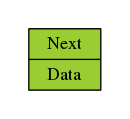
\includegraphics[width=0.2\textwidth]{Content/images/LL_Single_node.png}
\caption{Linked List Node Structure.}
\label{fig:LinkedListNodeStructure}
\end{figure}

The root node, as mentioned above, is special. It has no data part,
    only the pointer part, although it is not necessary for it not to be a full node, the data part will be empty in such cases.

The conceptual layout in memory is a bit like Figure~\ref{fig:ASimpleLinkedList} (using the
    addresses mentioned above and assuming the root node lives at address \$ABCD):

\begin{figure}[h]
\center
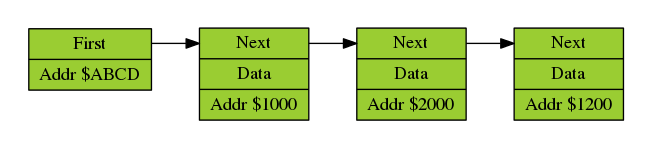
\includegraphics[width=0.95\textwidth]{Content/images/LL_Single_list.png}
\caption{A Simple Linked List.}
\label{fig:ASimpleLinkedList}
\end{figure}

The lowest section of each node above simply shows an example address in memory where that particular node lives. It is not part of the node itself.

In physical terms there are, of course, no handy arrows. Using real values as
    described above in the pointer locations, it would look like Figure~\ref{fig:MemoryOrganisationOfASimpleLinkedList}:

\begin{figure}[h]
\center
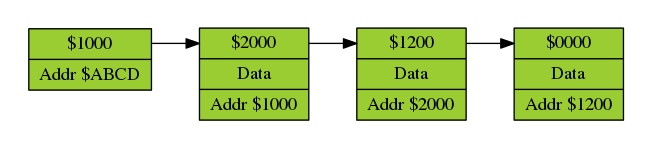
\includegraphics[width=0.95\textwidth]{Content/images/LL_Single_Memory.png}
\caption{Memory Organisation of a Simple Linked List.}
\label{fig:MemoryOrganisationOfASimpleLinkedList}
\end{figure}

You can see from \figurename~\ref{fig:MemoryOrganisationOfASimpleLinkedList} that the address of the following node is held in each node's first 4
    bytes. The address of FIRST is actually somewhere in your program
    and your program only needs to allocate storage for the 4 bytes it takes
    to hold the address of the initial node in the list. FIRST is, of course,
    the root node of the list.

You must store the value zero in there before you go off adding
    nodes, you'll see this reason why below in the code to add a node.

\subsection{Adding Nodes.}
\label{ch10-adding-nodes}%\hyperlabel{ch10-adding-nodes}%

Adding a new node is simple, you allocate it on the heap, fill in
      the data part and add it to the front of the list. It is far easier to
      add a node at the start -{} address 1000 in the above example -{} than to
      have to work through the entire list to find the current end, and then
      add it there. This method takes longer and longer to carry out as you
      add extra entries to the list. Adding at the start of the list takes the
      same time regardless of how many entries are in the list.

As you add each node to the list, you copy the value in FIRST into
      the new node's NEXT pointer and put the address of the new node into
      FIRST. Sounds complicated, but here it is in code. If we assume that
      A0.L has the address of FIRST and that A1.L has the address of the node
      to be inserted into the list, as contrivingly demonstrated by these two
      lines:

\begin{lstlisting}[firstnumber=1,caption={Adding a Node - Prelude},label={lst:AddingANodePrelude}]
Prelude    lea FIRST,a0        ; Pointer to storage of first node 
           lea NewEntry,a1     ; Address of new node
\end{lstlisting}

Then adding a new node to a list is as simple as this:

\begin{lstlisting}[firstnumber=last,caption={Adding a Node},label={lst:AddingANode}]
AddNode    move.l (a0),(a1)    ; Save first node in new node's NEXT
           move.l  a1,(a0)     ; Store new node in FIRST
           rts
\end{lstlisting}

Nothing to it. The new node is always added at the start of the
      list, so the value in FIRST always points to the most recently added
      node. As you need to have zero in the NEXT pointer of the final node in
      the list, you can see why it was important to initialise the value in
      your programs FIRST variable to zero before adding any nodes. If you
      didn't have zero, you'd never know when the list was finished.

One thing, you don't want to allow the user to add the root node
      to its own list at any time, so best change the above code to prevent
      this from happening.

\begin{lstlisting}[firstnumber=3,caption={A Better Way of Adding a Node},label={lst:BetterAddingANode}]
AddNode    cmpa.l  a0,a1       ; Don't allow the root node to be added
           beq.s   AddExit     ; Bale out quietly if attempted
           move.l (a0),(a1)    ; Save first node in new node's NEXT
           move.l  a1,(a0)     ; Store new node in FIRST
AddExit    rts
\end{lstlisting}

Another problem is when you try to add a node that is already
      there. So to be really careful, you could call the FindNode routine
      (coming soon -{} have patience!) prior to adding it in. However, as this
      scans the entire list until it finds or doesn't find the new node, it
      could add quite a lot of time to the simple exercise of adding a new
      node.

If you wrote the program, and you are allocating nodes on the heap
      each time, then don't bother attempting to find the node in the list
      before you add it.

\subsection{Deleting Nodes.}
\label{ch10-deleting-nodes}%\hyperlabel{ch10-deleting-nodes}%

Deleting a node is slightly more difficult. The node to be deleted
      could be anywhere in the list, or not even in the list. How to find the
      correct node is the main problem. However, for the same of argument,
      assume that we have the node address to be removed in A1.L and the
      address of FIRST in A0.L after a successful `find' operation, then
      removing the node at A1.L requires that we must navigate the list, as in
      the following explanation.

We must navigate the list because we don't know where in memory
      the node prior to the one we wish to delete is. We need to find it,
      because it has a NEXT pointer holding the address of the `deleted' node
      and this has to be changed or we lose everything in the list after the
      deleted node.

As ever, the value in the NEXT area of the very last node in the
      list is always zero. That way, we know when we have hit the end of the
      list. Here's the pseudo code to delete the node at A1.L from the list
      beginning at (A0.L)
\begin{itemize}[itemsep=0pt]

\item{}If the node to be deleted is the root node (the list pointer
          in A0) then don't allow it to be deleted.


\item{}Start of the main loop.


\item{}If the value stored in the address that A0.L points to is
          equal to zero, we have been passed an incorect node address to
          delete. Exit from the loop with an error.


\item{}If the value stored in the address that A0.L points to is not
          the same as the value in A1.L then copy the value in the address
          that A0.L points to into A0 and restart the main loop. Basically we
          have replaced the address in A0 with the NEXT address from the node
          we were just looking at.


\item{}If the value stored in the address that A0.L points to is
          equal to the value in A1.L then we have found the node PRIOR to the
          node we wish to delete and so the node we are looking at has to have
          the NEXT address updated to bypass the node we wish to delete so
          that it now points to the NEXT address which is currently stored in
          the node we are deleting. Exit from the loop with no errors.


\item{}End of main loop.

\end{itemize}

That's the pseudo code, here's the actual code. Using the same
      preliminary stuff as above to sort out initial values of A0.L and A1.L
      and a little bit extra to show whether errors have been detected or not,
      we begin with this:

\begin{lstlisting}[firstnumber=1,caption={Deleting a Node - Prelude},label={lst:DeletingANodePrelude}]
Prelude    lea FIRST,a0        ; Pointer to root node
           lea OldNode,a1      ; Address of node to delete
           moveq #ERR_EF,d0    ; End of file = node not found = error
\end{lstlisting}

Now, here's the actual code to find and remove the requested
      node.

\begin{lstlisting}[firstnumber=last,caption={Deleting a Node},label={lst:DeletingANode}]
DelNode    cmpa.l a0,a1        ; Don't allow the root node deletion
           beq.s DelExit       ; Bale out with error if attempted

DelLoop    cmp.l #0,(a0)       ; Reached the end yet?
           beq.s DelExit       ; Yes, node not found, exit with error

           cmp.l (a0),a1       ; Found the PRIOR node yet?
           bne.s DelNext       ; No, skip deletion code & try again

DelFound   move.l (a1),(a0)    ; PRIOR node NEXT = deleted node's NEXT 
           moveq  #0,d0        ; Node found and deleted ok
           bra.s  DelExit      ; Bale out with no errors

DelNext    move.l (a0),a0      ; A0 now holds the NEXT node in the list
           bra.s  DelLoop      ; Go around again

DelExit    tst.l d0            ; Set zero flag for success
           rts
\end{lstlisting}

The above code returns with the Z flag set if the node was deleted
      from the list, and unset if the node was not in the list. This allows
      the calling code to handle and errors correctly.

\subsection{Finding Nodes.}
\label{ch10-finding-nodes}%\hyperlabel{ch10-finding-nodes}%

The first thing you must do when deleting a node is to actually
      find it. The code above assumes that A1 holds a valid node address in
      the list defined by A0. Having said that, the code is robust enough to
      know that programmers make errors and it can handle the problem of a
      node address being passed which is not in the list by virtue of the fact
      that it scans the list until it finds the node prior to the one we wish
      to delete. It has to work that way because we need to adjust the NEXT
      pointer in the prior node to point past the deleted node to its NEXT
      node -{} if you catch my drift?

The code to find an node in a list is dependant on the sort of
      data stored in each node. If you store strings, the some form of string
      comparison routine needs to be built in -{} does it compare on an equality
      basis (`AAA' = `AAA') or nearly equal basis (`AAA' == `aaa') and so on.
      You can use the built in QDOSMSQ routines to do the comparisons.

If the data in the nodes are numbers (integers of word or long
      length) then you can compare them directly. If they are QDOSMSQ floating
      point format numbers, you can use the built in arithmetic routines to
      compare them. Regardless of which method is used, you need to write your
      own code to compare two nodes, or a node and a value so that the find
      routine knows when it has found the correct entry.

Of course, it is quite simple to build a FindNode routine which
      doesn't know or care what sort of data the individual nodes contain,
      provided it is passed the address of a routine which does know and care.
      If the specification for said routine requires the Z flag to be set for
      found and unset for not found, it could look something like the
      following peseudo code.

Assume that A0.L holds the address of FIRST, A1.L holds a pointer
      to a routine which compares the node with a given value and A2.L holds a
      pointer to that value. The data that A2.L points to can be anything, the
      routine at (A1.L) does the working out, our FindNode simply calls the
      routine once for each node in the list until such time as it gets a set
      Z flag on return. The comparison routine gets passed a node address in
      A3.L.
\begin{itemize}[itemsep=0pt]

\item{}Start of the main loop.


\item{}If the value stored in the address that A0.L points to is
          equal to zero, we have not found a node with the desired value. Exit
          the main loop with a NOT FOUND error.


\item{}Copy the address at (A0.L) into A3 and call the routine to
          compare data. If it returns with the Z flag set, the address in
          (A0.L) is the address of the node prior to the node we were looking
          for, however, the address in A3.L is the address of our required
          node as it is taken from the NEXT pointer. Remember, we passed the
          NEXT address (A0.L) over to the routine, not the address of THIS
          node -{} A0.L. Exit from the loop with the Z flag set to indicate a
          found node.


\item{}Copy the NEXT address from the node we are looking at into
          A0.L and go back to the start of the loop.


\item{}End of main loop.

\end{itemize}

And here's the real code to do the finding for use. As ever, we
      start off with some contrived values.

\begin{lstlisting}[firstnumber=1,caption={Finding a Node - Prelude},label={lst:FindingANodePrelude}]
Prelude    lea FIRST,a0        ; Pointer to root node address
           lea Compare,a1      ; Address of node comparison routine
           lea Required,a2     ; Address of the data we are looking for
           moveq #ERR_NF,d0    ; Node not found = error
\end{lstlisting}

Now, here's the actual code to find a node in the list which holds
      the required value.

\begin{lstlisting}[firstnumber=last,caption={Finding a Node},label={lst:FindingANode}]
FindNode   cmp.l #0,(a0)       ; Reached the end yet?
           beq.s DelExit       ; Yes, node not found, exit with error

           move.l (a0),a3      ; Fetch the NEXT node address into A3.L
           jsr (a1)            ; And jump into the comparison routine
           beq.s FindFound     ; Looks like we found our node

FindNext   move.l (a0),a0      ; A0 now holds the NEXT node in the list
           bra.s  FindNode     ; Go around again

FindFound  moveq  #0,d0        ; Clear the error flag

FindExit   tst.l d0            ; Set zero flag for success
           rts
\end{lstlisting}

The following is an example of a compare routine to look at a long
      word of data in the node at (A3.L) and see if it is equal to the long
      word of data stored at (A2.L). Don't forget, the comparison routine must
      preserve A0, A1, A2 and D0 or it will all go horribly wrong. The
      following routine does exactly that, by the simple method of not
      actually using those registers at all!

\begin{lstlisting}[firstnumber=1,caption={Finding a Node - Data Comparison},label={lst:FindingANodeDataComparison}]
NData   equ 4                  ; Offset to node's data part

Compare    cmp.l NData(A3),(A2) ; Is the data = the value we want?
           rts                 ; Exit with Z set if so
\end{lstlisting}

If an attempt is made to find the root node, then it will
      fail.

So there you have three short but extremely powerful routines
      which make linked lists possible. At this point I have to mention that
      there are actually routines built into QDOSMSQ to do exactly the same
      work as the AddNode and DelNode routines above, but there is nothing
      like FindNode -{} which is a shame. However, you now know how to build
      linked lists and add and delete nodes. You also know how to find an
      entry in a linked list so that you can process it in some way.

\subsection{The Code Wrapper.}\index{Linked Lists!Test Harness}
\label{ch10-code-wrapper}%\hyperlabel{ch10-code-wrapper}%

Putting all of the above together and tying in some extras to
      allocate nodes etc, here is a small, but perfectly formed program to
      create a linked list. The following is a wrapper that we shall use to
      demonstrate first the single linked lists as explained above. Later on,
      when other types of linked list are explained, we shall drop in only the
      code we need for the demo

\begin{lstlisting}[firstnumber=1,caption={Linked Lists - Wrapper - Part 1},label={LinkedListsWrapperPart1}]
* =====================================================================
* A test harness 'job' for our linked lists code. What's the point of
* all the explanations if you can't test the code?
*
* This code is simply a wrapper to allow different demos to be slotted
* in to demonstrate the real code in the chapter, as opposed to the job
* code.
*
* The code being demonstrated is located at DEMO below. As new demos
* are required, only that bit should (!) need changing.
* =====================================================================

* ---------------------------------------------------------------------
* These are offsets from the start of the job's dataspace where working
* variable are stored. The dataspace is held at (A4) in the job's code.
* ---------------------------------------------------------------------
con_id      equ     0                   ; Id for title channel
con_id2     equ     4                   ; Id for main output

* ---------------------------------------------------------------------
* These are simply user friendly names instead of numbers for various
* bits and bobs, colours etc.
* ---------------------------------------------------------------------
black       equ     0                   ; Colour code for mode 4 black
red         equ     2                   ; Red
green       equ     4                   ; Green
white       equ     7                   ; White
linefeed    equ    10                   ; Linefeed character
oops        equ    -1                   ; General error code
err_nc      equ    -1                   ; NOT COMPLETE error code

* ---------------------------------------------------------------------
* Constants for use with job control commands. (It doesn't matter if I
* have two names with the same value! )
* ---------------------------------------------------------------------
infinite    equ     -1                  ; Infinite timeout
me          equ     -1                  ; Id for 'this' job


* ---------------------------------------------------------------------
* Code starts here.
* ---------------------------------------------------------------------
start       bra.s   LinkList            ; 2 bytes short jump
            dc.l    0                   ; 4 bytes padding
            dc.w    $4afb
            dc.w    11                  ; Bytes in job's name
            dc.b    'LinkedLists',0     ; Bytes of job's name + padding

LinkList    adda.l   a6,a4              ; A4.L = start of dataspace
            bsr      Mode4              ; Set the screen mode
            bsr      Title              ; Open the title window
            bsr      Output             ; Open the output window
            bsr      Headings           ; Display headings
            bsr      Demo               ; Do the demo code
            bsr      Finished           ; Advise user that we are done

* ---------------------------------------------------------------------
* Code ends here.
* ---------------------------------------------------------------------
all_done    moveq   #mt_frjob,d0        ; Force Remove a job
            moveq   #me,d1              ; The current job
            move.l  d0,d3               ; Error code for SuperBasic
            trap    #1                  ; Kill this job

            bra.s   all_done            ; Should never get here
\end{lstlisting}

\begin{note}
The following code will be replaced by either the singly linked
        list or the doubly linked list demo code which follows at the end of
        this chapter. For now, however, it is a place holder.
\end{note}

\begin{lstlisting}[firstnumber=last,caption={Linked Lists - Wrapper - Demo Placeholder},label={LinkedListsWrapperDemoPlaceholder}]
* ---------------------------------------------------------------------
* The DEMO code starts here.
* ---------------------------------------------------------------------
Demo        rts

* ---------------------------------------------------------------------
* The DEMO code ends here.
* ---------------------------------------------------------------------
\end{lstlisting}

\begin{note}
The following code is common to both demos.
\end{note}

\begin{lstlisting}[firstnumber=last,caption={Linked Lists - Wrapper - Part 2},label={LinkedListsWrapperPart2}]
* ---------------------------------------------------------------------
* Set mode 4 if not already set. Do not change from TV to monitor or
* vice versa. We must preserve the display type if we reset the mode.
* ---------------------------------------------------------------------
Mode4       moveq    #mt_dmode,d0
            moveq    #-1,d1             ; Read current mode
            moveq    #-1,d2             ; Read current display type
            trap     #1                 ; Do it
            tst.l    d0                 ; Did it work?
            bne      all_done           ; No, bale out, cannot continue

            tst.b    d1                 ; 0 in D1.B = Mode 4
            beq.s    ModeExit           ; No need to set mode 4
            moveq    #mt_dmode,d0
            clr.l    d1                 ; We need mode 4
            trap     #1                 ; Set mode 4 (d2 = disp type)
            tst.l    d0                 ; Check it
            bne      all_done           ; Bale out if errors detected
ModeExit    rts                         ; Done.

* ---------------------------------------------------------------------
* Mode 4 is in use. Open the title window at the top of the screen.
* ---------------------------------------------------------------------
Title       lea      con_def,a1         ; Window definition
            movea.w  ut_con,a2          ; Utility to define a window
            jsr      (a2)               ; Do it
            tst.l    d0                 ; Did it work ok?
            bne      all_done           ; No, exit program
            move.l   a0,con_id(a4)      ; Store title channel id
            rts                         ; Done

*----------------------------------------------------------------------
* Definition for title window channel
*----------------------------------------------------------------------
con_def     dc.b    red                 ; Border colour
            dc.b    1                   ; Border width
            dc.b    white               ; Paper/strip colour
            dc.b    black               ; Ink colour
            dc.w    448                 ; Width
            dc.w    24                  ; Height
            dc.w    32                  ; Start position x
            dc.w    16                  ; Start position y

* ---------------------------------------------------------------------
* Open the output window underneath the title one.
* ---------------------------------------------------------------------
Output      lea      con_def2,a1        ; Output window definition
            movea.w  ut_con,a2          ; Utility again
            jsr      (a2)               ; Do it
            tst.l    d0                 ; Did it work?
            bne      all_done           ; No, exit routine
            move.l   a0,con_id2(a4)     ; Store output channel id

            moveq    #0,d0              ; No errors detected
            rts

*----------------------------------------------------------------------
* Definition for output window channel
*----------------------------------------------------------------------
con_def2    dc.b    red                 ; Border colour
            dc.b    1                   ; Border width
            dc.b    white               ; Paper/strip colour
            dc.b    black               ; Ink colour
            dc.w    448                 ; Width
            dc.w    200                 ; Height
            dc.w    32                  ; X org
            dc.w    40                  ; Y org

* ---------------------------------------------------------------------
* Print the headings
* ---------------------------------------------------------------------
headings    movea.l  con_id(a4),a0       ; Title channel id
            bsr.s    cls                 ; Clear screen
            lea      mes_title,a1        ; Title string
            bsr.s    prompt              ; Print title string
            rts

mes_title   dc.w     mes_end-mes_title-2
            dc.b     'Single Linked Lists'
mes_end     equ      *

* ---------------------------------------------------------------------
* Sign off message
* ---------------------------------------------------------------------
Finished    movea.l  con_id2(a4),a0      ; Title channel id
            lea      end_title,a1        ; Title string
            bsr.s    prompt              ; Print title string
            bsr.s    input               ; Wait for ENTER
            rts

end_title   dc.w     end_end-end_title-2
            dc.b     linefeed,linefeed,'Press ENTER to quit: '
end_end     equ      *

* =====================================================================
* CLS:
* =====================================================================
* 1. Clear the (screen) channel whose id is in A0.
* =====================================================================
cls         moveq    #sd_clear,d0        ; CLS
            moveq    #infinite,d3        ; Infinite timeout
            trap     #3                  ; CLS title window
            rts

* =====================================================================
* Prompt:
* =====================================================================
* 1. Print the string at (A1) to the channel in A0.
*
* Z set if all ok, unset if not.
* =====================================================================
prompt      movea.w ut_mtext,a2          ; Print a string utility
            jsr     (a2)                 ; Print it
            tst.l   d0                   ; Check for errors
            rts

* =====================================================================
* Input:
* =====================================================================
* Wait for user input from the channel id in A0.
*
* Returns the input length (not counting the ENTER character) in D1.W
* Returns the address of the first character in the buffer in A1.L
* Preserves the channel id in A0.L
* Z set if all ok, unset if not.
* =====================================================================
input       lea     buffer+2,a1         ; Our buffer address plus 2
            move.l  a1,-(a7)            ; Save it on the stack
            moveq   #io_fline,d0        ; Input some bytes (+ linefeed)
            moveq   #60,d2              ; Buffer size maximum
            moveq   #infinite,d3        ; Inifinite timeout
            trap    #3

            move.l  (a7)+,a1            ; Restore buffer pointer
            subq.w  #1,d1               ; Subtract the linefeed
            move.w  d1,-2(a1)           ; Store length in buffer
            tst.l   d0                  ; Did it all work?
            rts

buffer      ds.w    31                  ; 60 chars for input + 1 word

* =====================================================================
* hex_l:
* =====================================================================
* Convert a 4 byte value in D4.L to Hex in a buffer. Use the input
* buffer for the output and DOES NOT store the length word!
*
* Expects D4.L to hold the value.
* =====================================================================
hex_l       swap    d4              ; $ABCD -> $CDAB in D4
            bsr.s   hex_w           ; Convert the $AB part first
            swap    d4              ; $CDAB -> $ABCD again
*           drop into hex_w to convert the $CD part

* =====================================================================
* hex_w:
* =====================================================================
* Convert a 2 byte value in D4.W to Hex in a buffer.
*
* Expects D4.W to hold the value.
* Expects A1.L to point at the buffer.
* =====================================================================
hex_w       ror.w   #8,d4           ; $DE -> $ED in D4
            bsr.s   hex_b           ; Convert the $D part first
            rol.w   #8,d4           ; $ED -> $DE again
*           drop into hex_b to convert the $E part

* =====================================================================
* hex_b:
* =====================================================================
* Convert a 1 byte value in D4.B to Hex in a buffer.
*
* Expects D4.B to hold the value.
* Expects A1.L to point at the buffer.
* =====================================================================
hex_b       ror.b   #4,d4           ; Swap lower and higer nibbles
            bsr.s   hex_nibble      ; Print high nibble first
            rol.b   #4,d4           ; Swap back again
*           drop into hex_nibble to print the lower nibble

* =====================================================================
* hex_nibble:
* =====================================================================
* Convert a 4 bit value in D4.B to Hex in a buffer.
*
* Expects D4.B to hold the value.
* Expects A1.L to point at the buffer.
* =====================================================================
hex_nibble  move.b  d4,-(a7)        ; Save value in both nibbles
            andi.b  #$0f,d4         ; D4.B now = 0 to 15
            addi.b  #'0',d4         ; Now = '0' to '?' (ascii only)
            cmpi.b  #'9',d4         ; Is this a digit?
            bls.s   nib_digit       ; Yes
            addi.b  #7,d4           ; Add offset to UPPERCASE letters

nib_digit   move.b  d4,(a1)+        ; Store in buffer
            move.b  (a7)+,d4        ; Restore original value
            rts

* =====================================================================
* print_hex:
* =====================================================================
* Convert D4 into 8 hex characters, and print it to the channel in A0.L
*
* Expects D4.L to hold the value.
* Expects A0.L to hold the channel id.
* =====================================================================
print_hex   lea      buffer,a1      ; Output buffer for address
            move.w   #8,(a1)+       ; We know the result is 8 bytes
            bsr      hex_l          ; Convert 4 bytes to text
            lea      buffer,a1      ; Text to print
            bsr      prompt         ; Print it
            rts                     ; All done. (Error code in D0)

* =====================================================================
* End of test harness
* =====================================================================
\end{lstlisting}

\subsection{Running The Wrapper Code.}
\label{ch10-single-list}%\hyperlabel{ch10-single-list}%

The above code does absolutely nothing, but if you assemble it and
      exec the resulting file, you should see a pair of windows one with a
      message `Single Linked Lists' and a prompt in the other to `Press ENTER
      to quit'. Once you press the ENTER key, the job will finish. So far so
      good.

The reason that it does nothing is shown below:

\begin{lstlisting}[firstnumber=1,caption={Linked Lists - Wrapper - Demo Placeholder},label={LinkedListsWrapperDemoPlaceholder2}]
* =====================================================================
* The DEMO code starts here.
* =====================================================================
Demo        rts

* =====================================================================
* The DEMO code ends here.
* =====================================================================
\end{lstlisting}

The code at Demo, does nothing but return to the caller. Our
      linked list code will be slotted in to replace the lines of code shown
      above.

To demonstrate linked lists, we need only add some code to replace
      the lines above. In the following two chapters we do just that, and code
      to demonstrate single and doubly linked lists follows there. 

\subsection{Problem Areas.}
\label{ch10-problems}%\hyperlabel{ch10-problems}%

The above description, and code, is for a Single Linked List, so
      called because there is a single link in each node which points to the
      next entry in the list. This is simple to code up -{} as we have seen -{}
      and is fairly simple to understand, at least it is if I've done my job
      correctly.

The problem with a linked list created in the above fashion is
      that you always have to scan the list from start to some undetermined
      entry when you want to delete a node. And this can add serious delays to
      the processing of your application when a lot of nodes have to be
      traversed each time you need to delete one.

There is an answer, Doubly Linked Lists.

\section{Doubly Linked Lists.}
\label{ch10-double-lists}%\hyperlabel{ch10-double-lists}%

If we change the structure of our nodes and add a PRIOR pointer to
    each node and to the root node as well, we can store the address of both
    nodes neighbouring our current one, as shown in  Figure~\ref{fig:StructureOfADoubleLinkedListNode} which shows the node structure.
    
\begin{note}
Simon N Goodwin pointed out some time ago that there is no need to have two separate pointers for prior and next nodes in the linked list, only one pointer is needed.

This pointer holds the address of both pointers \opcode{EOR}'d together. To extract the prior pointer, simply \opcode{EOR} it with the next address and vice versa.

This assumes that you know the address of the prior and/or next pointer I suspect!
\end{note}    

\begin{figure}[h]
\center
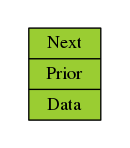
\includegraphics[width=0.2\textwidth]{Content/images/LL_Double_node.png}
\caption{Structure of a Doubly Linked List Node.}
\label{fig:StructureOfADoubleLinkedListNode}
\end{figure}

Our conceptual model of the doubly linked list is shown in Figure~\ref{fig:ConceptualModelOfADoublyLinkedList}.

\begin{figure}[h]
\center
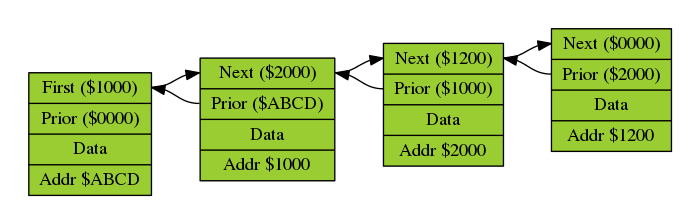
\includegraphics[width=0.95\textwidth]{Content/images/LL_Double_list.png}
\caption{Conceptual Model of a Doubly Linked List.}
\label{fig:ConceptualModelOfADoublyLinkedList}
\end{figure}

\subsection{Adding Nodes.}
\label{ch10-dbl-adding-nodes}%\hyperlabel{ch10-dbl-adding-nodes}%

Adding a new node is still simple. Having allocated a node on the
      heap, you set its PRIOR pointer to zero and its NEXT to the current
      address held in the FIRST pointer -{} almost identical to the single
      linked list code above.

\begin{lstlisting}[firstnumber=1,caption={Adding a Node - Prelude},label={lst:AddingANodePrelude2}]
Prior      equ 4               ; Offset to PRIOR pointer in a node

Prelude    lea FIRST,a0        ; Pointer to root node
           lea NewEntry,a1     ; Address of new node
\end{lstlisting}

Then adding a new node to a doubly linked list is as simple as
      this:

\begin{lstlisting}[firstnumber=last,caption={Adding a Node},label={lst:AddingANode2}]
AddNode    cmpa.l  a0,a1         ; Don't add the root node again
           beq.s   AddExit       ; Bale out quietly if attempted
           move.l (a0),(a1)      ; Save first node in new node's NEXT 
           move.l  a0,Prior(a1)  ; Set the PRIOR node for this new node
           move.l  a1,(a0)       ; Store new node in FIRST 
           move.l  (a1),a0       ; A0 = address of original FIRST node
           cmpa.l  #0,a0         ; Nothing to do if A0 is zero
           beq.s   AddExit       ; Z set = First node added
           move.l  a1,prior(a0)  ; Store new FIRST node
AddExit    rts
\end{lstlisting}

As with single linked lists there is nothing to it. The new node
      is always added at the start of the list, so the value in FIRST always
      points to the latest node added. The first non root node in a doubly
      linked list has no real PRIOR node, so that part of the newly added node
      is simply set to point back at the root node.

Building up the linked list above, in Figure~\ref{fig:ConceptualModelOfADoublyLinkedList}, in stages, we would start with the root node located, most likely, somewhere in our code itself. Initially both the next and prior pointers would be set to zero.

The nodes are address at the start of the list, so the first node to be added would be the one on the far right of the diagram, node \$1200. That node would be created and added to the list by setting the root node's next pointer to address \$1200 and the new node's prior pointer to address \$ABCD. Because it is the final node in the list so far, its next pointer is set to zero.

After adding the node at address \$2000, we would change the next pointer of the root node to this new address, \$2000, and the prior pointer of the node at \$1200 to \$2000. The new node would have its prior pointer set to the address that was in the \$1200 node's prior pointer, which is \$ABCD.

This process is repeated as we create each new node and add it to the list. Eventually, we end up with the structure shown in Figure~\ref{fig:ConceptualModelOfADoublyLinkedList} above.

You can see how each node points onward to the NEXT one and also
      backwards to the PRIOR one. The last node has no NEXT nodes, so it has
      its NEXT pointers set to zero to indicate the end of the list.

\subsection{Deleting Nodes.}
\label{ch10-dbl-deleteing-nodes}%\hyperlabel{ch10-dbl-deleteing-nodes}%

Deleting a node is much simpler. There is no need to scan the
      entire list from the start looking for the node prior to the one you
      want to delete because you already know its address by following the
      PRIOR pointer backwards from the node to be deleted.

Here's the pseudo code to delete a node. We assume, as before,
      that A0.L is the root node pointer and A1.L is the node to be
      deleted.
\begin{itemize}[itemsep=0pt]

\item{}If the two addresses are equal, we cannot allow the root node
          to be deleted, exit with an error.


\item{}If the address in the root node's NEXT pointer is zero then we
          still have an empty list so the value in A1 must be illegal. Exit
          with an error.


\item{}Fetch the deleted node's PRIOR pointer. Every real node in a
          list will have a valid PRIOR pointer, only the root node has no
          prior pointer and we don't allow that to be deleted.


\item{}Store the NEXT pointer from the deleted node into the NEXT
          pointer of the prior node.


\item{}Fetch the deleted node's NEXT pointer, which might be zero if
          we are deleting the final node in the list.


\item{}If it is not zero, store the deleted node's PRIOR pointer in
          the next node's PRIOR pointer.


\item{}Exit without error.

\end{itemize}

That's the pseudo code, here's the real code to do all of the
      above.

\begin{lstlisting}[firstnumber=1,caption={Deleting a Node - Prelude},label={lst:DeletingANodePrelude2}]
Prior      equ 4               ; Offset to PRIOR pointer in each node

Prelude    lea FIRST,a0        ; Pointer to root node
           lea OldNode,a1      ; Address of node to delete
           moveq #ERR_BP,d0    ; Trying to delete the root node?
\end{lstlisting}

Now, here's the actual code to find and remove the requested
      node.

\begin{lstlisting}[firstnumber=last,caption={Deleting a Node},label={lst:DeletingANode2}]
DelNode    cmpa.l a0,a1        ; Don't delete the root node
           beq.s DelExit       ; Bale out with error if attempted

           cmp.l #0,(a0)       ; Do we actually have a list?
           beq.s DelExit       ; Yes, node not found, exit with error

           move.l Prior(a1),a0 ; Fetch the deleted node's PRIOR pointer
           move.l (a1),(a0)    ; Store its NEXT pointer in the NEXT
                               ; pointer of the PRIOR node

           move.l (a1),a0      ; Fetch the deleted node's NEXT pointer
           move.l  Prior(a1),Prior(a0) ; Store its PRIOR pointer in the
                                       ; next node's PRIOR pointer.

DelFound   move.l (a1),(a0)    ; PRIOR's NEXT = the deleted node's NEXT
           moveq  #0,d0        ; Node deleted ok
           bra.s  DelExit      ; Bale out with no errors

DelNext    move.l (a0),a0      ; A0 now holds the NEXT node in the list
           bra.s  DelNode      ; Go around again

DelExit    tst.l d0            ; Set zero flag for success
           rts
\end{lstlisting}

\subsection{Finding Nodes.}
\label{ch10-dbl-finding-nodes}%\hyperlabel{ch10-dbl-finding-nodes}%

As with single linked lists, you may have a need to locate a
      specific node by its contents, so you need a generic FindNode routine
      again. The fact that the list has two pointers this time around is the
      only difference, so the code is basically the same as for the single
      linked list above.

The only difference is the offset to the data part of the node
      needs to be set to 8 bytes instead of 4, so while the code for the
      FindNode remains the same, the code for the Compare routine needs to be
      changed to the following to account for the extra pointer.

As before, the comparison routine must preserve A0, A1, A2 and D0
      or it will all go horribly wrong.

\begin{lstlisting}[firstnumber=1,caption={Finding a Node - Data Comparison},label={lst:FindingANodedataComparison2}]
NData   equ 8                  ; Offset from start of node to the data

Compare    cmp.l NData(a3),(a2) ; Is the data = the value we want?
           rts                  ; Exit with Z set if so
\end{lstlisting}

Again, if an attempt is made to `find' the root node, then it will
      fail.

\subsection{A Better Mousetrap.}
\label{ch10-better-mousetrap}%\hyperlabel{ch10-better-mousetrap}%

Because the code for the linked list find routine is identical
      except for the offset in the compare routine you can use the same code.
      If you modify it so that it passes the offset over to the compare
      routine in a spare register, say D1.W for example, then you can even
      have the same compare routine for both single and doubly linked lists,
      as shown below.

\begin{lstlisting}[firstnumber=1,caption={Finding a Node - Data Comparison},label={lst:FindingANodedataComparison3}]
Compare    cmp.l 0(a3,d1.w),(a2) ; Is the data = the value we want?
           rts                   ; Exit with Z set if so
\end{lstlisting}

Another method, much loved in the internals of Microsoft Windows,
      is to store a word holding the offset to the data at the start of each
      node. This would remove the need for the D1.W register to be passed into
      the comparison routine as a parameter as it could easily extract the
      data from the node itself, as follows:

\begin{lstlisting}[firstnumber=1,caption={Finding a Node - Alternative Data Comparison},label={lst:FindingANodedataComparison4}]
Compare    move.w (a3),d1        ; Fetch the offset to the data
           cmp.l 0(a3,d1.w),(a2) ; Is the data = the value we want?
           rts                   ; Exit with Z set if so
\end{lstlisting}

The drawback to this method is the redundancy of the data -{} each
      and every node has to have the first two bytes set to the offset to the
      data plus 2 for the size of the offset word itself. Two extra bytes per
      node may be the difference between getting all the data in memory or
      not. It is, of course, always up to you. If you decide to go down this
      route, don't forget to amend the code to add, find and delete nodes to
      take the extra two bytes into consideration when manipulating the
      pointers to NEXT and PRIOR. Your root node must also reflect these
      changes and have an offset word added to its own structure.

You might see a need to build a couple of comparison routines to
      compare two nodes rather than the example above where a node is being
      compared with a value. On the other hand, you could simply write one
      routine to compare two nodes and when looking for a value, create a
      dummy node and use that in the comparison routine. That way, you don't
      need separate routines to compare values and nodes.

\subsection{Double Trouble.}
\label{ch10-double-trouble}%\hyperlabel{ch10-double-trouble}%

The problem with a doubly linked list is that while adding nodes
      is just as simple as before, but deleting them could be problematical.
      If you are passed the address of a node which is not in the list, how do
      you tell that it is or is not a valid node address? You can end up
      trashing bytes of memory almost at random as you start changing the NEXT
      and PRIOR pointers for two areas of memory which may not be in your
      list.

My solution is to use a flag word or long word after the two list
      pointers in each node and when passed in a node address to delete,
      compare this value in the flag to see if it is correct before attempting
      to delete the node. As ever, I leave this `as an exercise for the
      reader' to modify the code above to carry out said checks.

\subsection{Sorting Lists.}
\label{ch10-sorting-lists}%\hyperlabel{ch10-sorting-lists}%

The best way to sort a list is not to have to sort it at all. When
      you store a node in the list, store it in the correct place according to
      its value. A doubly linked list is used here again as you will need to
      go NEXT until you hit a value greater than the one you want to insert,
      then you might need to go PRIOR to insert it in the correct location.
      I'll leave you to figure out that little exercise.

There is an another way, which involves TREES of nodes rather than
      lists. A tree is simply a linked list which has a LEFT, RIGHT and UP
      pointer in each node.

With a tree, the nodes are not in a long line, but they are off to
      the LEFT and RIGHT of the root node. Each node may itself have children
      to the LEFT and RIGHT as well as a parent found by following the UP
      pointer.

Unfortunately, trees are a bit beyond my skills at the moment. I
      remember doing them in college and learning all the different ways to
      navigate them, but I cannot remember much about them nowadays -{} it's
      been over 30 years since I last considered them.

\section{Remember those arrays?}
\label{ch10-remember-arrays}%\hyperlabel{ch10-remember-arrays}%

Way back at the start of this chapter, I mentioned arrays and their
    problems. Well, combining an array with a linked list could be useful -{}
    but remember, the array is limited by the fact that you have to pre-{}define
    the number of entries.

Bearing this in mind, you could allocate an array of, say 1000
    entries of 4 bytes each. Each entry in the array holds the address of an
    individual node, not the actual data stored there. Our address book system
    of 100 byte strings (not much of an address book I admit!) will now only
    need about 4Kb plus 102 bytes per used node -{} including the string length
    word for each entry. Using a plain array it would need almost 102Kb even
    for a blank address book.

Now you have compromised on memory needs as you don't allocate the
    space required to store your data until you need to, and you do allocate a
    much smaller amount to hold the `contents table'. As you create new nodes,
    add their address to the array. You can still use the single or double
    linked lists if you wish, but there is no need. The array holds all the
    locations of each node in the order that they were created and you can
    navigate forwards, backwards and even access nodes at random using this
    method because the formula to find a given node is once more
    usable.

Have fun trying that out!

\section{Coming Up...}
\label{ch10-the-end}%\hyperlabel{ch10-the-end}%

Coming up next, the real code for the single linked list demo, and
    following that, the code for the doubly linked list demo.



\chapterimage{chapter_head_2.pdf} % Chapter heading image
\chapter{Single Linked Lists Demo Code}
\index{Linked Lists!Single Link - Demo Code}
 
\section{Introduction}
\label{ch11-intro}%hyperlabel{ch11-intro}%

The following code demonstrates the use of single linked lists. It
    should be slotted into the test harness code wrapper in Chapter 10 at the
    appropriate place. It cannot be assembled as it stands -{} it needs to be
    part of the test harness.

\section{How Does The Code Work?}
\label{ch11-single-code}%hyperlabel{ch11-single-code}%

The code is a small example of creating and navigating a linked
    list. The demo starts by creating a list of 5 nodes, each holding one long
    word of data being simply the node number 0 to 4.

The list contents are then printed on the screen showing the node
    address, the next pointer and the data stored in that node. Once this is
    done, the node with data contents of 3 is located and deleted prior to the
    new list being printed out again.

Finally, each node in the list is deleted.

The first part of the code simply controls the whole demo by calling
    various sub-{}routines to do the hard work, display messages etc on
    screen.

\begin{lstlisting}[firstnumber=1,caption={Single Linked List - Demo Code}]
* =====================================================================
* The DEMO code starts here.
*
* This demo does the following:
*
* Creates a number of nodes and stores a LONG value in each one.
* Lists each node address, its NEXT pointer and data value on screen.
* Deletes a node.
* Lists each node address, its NEXT pointer and data value on screen.
* Finds a node based on its data and displays its details on screen.
* Deletes all the nodes from the list.
* =====================================================================
Demo       bsr     BuildList            ; Build a linked list
           bsr     Before               ; Display 'BEFORE:'
           bsr     ShowList             ; Display list details
           bsr     FindNode             ; Locate a single node
           bne.s   DemoAfter            ; Failed to find node data = 3
           bsr     DeleteNode           ; Delete a single node

DemoAfter  bsr     After                ; Display 'AFTER: '
           bsr     ShowList             ; Show details again
           bsr     KillList             ; Delete entire list
           rts                          ; Done
\end{lstlisting}

Following on from the main control section of the demo, we have our
    much beloved root node which must be initialised to zero as outlined in
    the original article. This is the pointer we will be loading into A0 quite
    often in the demo and it holds the address of the first node in the list.
    At present, there is no list, so the contents are set to zero to indicate
    the very end of the list.

\begin{lstlisting}[firstnumber=last,caption={Single Linked List - Demo Code - Root Node}]
* ---------------------------------------------------------------------
* A location to hold a single long word pointing to the first 'real'
* node in our linked list. This must be initialized to zero.
* ---------------------------------------------------------------------
RootNode   dc.l    0                    ; This is our root node.
\end{lstlisting}

The first of our sub-{}routines follows on. This part builds a list of
    5 nodes in the most simple manner possible -{} it runs a loop which calls
    the sub-{}routine to create a single node and link it into the list. If you
    want a bigger list, change the counter loaded into D7 to one less than the
    number of nodes you want. Don't forget to adjust the height of your window
    as well if you want to see all the results on screen at the same
    time.

\begin{lstlisting}[firstnumber=last,caption={Single Linked List - Demo Code - Build List}]
* ---------------------------------------------------------------------
* Build a list of 5 nodes each holding a long word of data.
* ---------------------------------------------------------------------
BuildList  lea     RootNode,a0          ; Pointer to root node address
           moveq   #4,d7                ; How many nodes in D7 = 5
           moveq   #8,d1                ; Each node is 8 bytes long

BuildLoop  bsr.s   BuildNode            ; Create a node, address in A1
           bne     all_done             ; Just die on errors
           move.l  d7,4(a1)             ; Store data value
           bsr.s   AddNode              ; Add to list
           dbra    d7,BuildLoop         ; Do the rest
           rts                          ; Done
\end{lstlisting}

Here's the first of the real list routines. We add a new node into
    the list in the manner outlined in the article. We reject attempts to add
    the root node into the list -{} but without flagging any errors -{} and, as
    explained, we don't attempt to check if the new node already exists in the
    list because we are creating the node on the heap, so the chances of the
    new node being present already are pretty slim to say the least.

\begin{lstlisting}[firstnumber=last,caption={Single Linked List - Demo Code - Add Node}]
* ---------------------------------------------------------------------
* AddNode - Adds a new node to a list. See text for details.
* Preserves all regsiters.
* No errors returned.
* ---------------------------------------------------------------------
AddNode    cmpa.l  a0,a1                ; Don't add the root node again
           beq.s   AddExit              ; Bale out quietly if attempted
           move.l (a0),(a1)             ; Save first node in new NEXT
           move.l  a1,(a0)              ; Store new node in root node
AddExit    rts
\end{lstlisting}

A new node is built by allocating some space on the common heap but
    we must preserve the working registers, the following code does this for
    us.

\begin{lstlisting}[firstnumber=last,caption={Single Linked List - Demo Code - Build Node}]
* ---------------------------------------------------------------------
* Allocate a single new node
* On entry, D1.L is amount of memory required.
* On exit, A1 holds the address of the new node, with D0 holding errors.
* All registers preserved - unless otherwise stated.
* ---------------------------------------------------------------------
BuildNode  movem.l d1-d3/a0/a2-a3,-(a7) ; Save working registers
           moveq   #MT_ALCHP,d0         ; Set the trap
           moveq   #me,d2               ; I want it for me
           trap    #1                   ; Do it
           move.l  a0,a1                ; Node address into A1
           movem.l (a7)+,d1-d3/a0/a2-a3 ; Restore working registers
           tst.l   d0                   ; Set flags
           rts                          ; Exit
\end{lstlisting}

The following sub-{}routine is called once to display the linked list
    before we do the deletions and again after we have deleted a node. The
    code simply walks through the entire list and prints out the node address,
    the next pointer and the data value by calling other sub-{}routines.

\begin{lstlisting}[firstnumber=last,caption={Single Linked List - Demo Code - Show List}]
* ---------------------------------------------------------------------
* Walk through a linked list displaying the details of each node as we
* go.
* On entry, A0 = root node of the list.
* ---------------------------------------------------------------------
ShowList    lea    RootNode,a0          ; Root node address

ShowLoop    move.l (a0),a0              ; Get address of the next node
            cmpa.l #0,a0                ; Done?
            beq.s  ShowExit             ; Yes
            move.l a0,-(a7)             ; Preserve A0 - it's our node
            bsr.s  ShowNode             ; Display that node's details
            move.l (a7)+,a0             ; Restore the node pointer 
            bra.s  ShowLoop             ; Do the rest of the list

ShowExit    rts                         ; Done
\end{lstlisting}

This next short routine is called with the address of a node in A0.L
    and prints the details of that node to the screen.

\begin{lstlisting}[firstnumber=last,caption={Single Linked List - Demo Code - Show Node}]
* ---------------------------------------------------------------------
* Display the details of a single node in the linked list.
* On entry A0 = the node address.
* ---------------------------------------------------------------------
ShowNode    move.l a0,a5                ; The node address
            move.l con_id2(a4),a0       ; The channel address
            move.l a5,d4                ; The node address
            bsr.s  ShowAddr             ; Print node address
            move.l (a5),d4              ; The NEXT pointer
            bsr.s  ShowNext             ; Print NEXT pointer
            move.l 4(a5),d4             ; The node data
            bsr    ShowData             ; Print the data
            rts
\end{lstlisting}

Obviously, just displaying the list contents isn't very user
    friendly, so the next couple of routines display a title which informs
    the user if the list being displayed is `before' or `after' the deletion
    of a node.

\begin{lstlisting}[firstnumber=last,caption={Single Linked List - Demo Code - Show Before and After States}]
* ---------------------------------------------------------------------
* Display 'BEFORE:' in the output channel.
* ---------------------------------------------------------------------
Before     lea     BeforeAddr,a1        ; The prompt
           movea.l con_id2(a4),a0       ; Needs channel id
           bsr     Prompt               ; Print it
           rts

BeforeAddr dc.w    B4End-BeforeAddr-2
           dc.b    'BEFORE:',linefeed
B4End      equ     *

* ---------------------------------------------------------------------
* Display 'AFTER:' in the output channel
* ---------------------------------------------------------------------
After      lea     AfterAddr,a1         ; The prompt
           movea.l con_id2(a4),a0       ; Needs channel id
           bsr     Prompt               ; Print it
           rts

AfterAddr  dc.w    AftEnd-AfterAddr-2
           dc.b    linefeed,linefeed,'AFTER:',linefeed
AftEnd     equ     *
\end{lstlisting}

There now follows one of three separate but short routines to
    display on screen, the various parts of a list node. This one simply
    displays the node's address in memory. Following after this routine is a
    number of small sub-{}routines which assist in the displaying of node data
    by converting the contents of D4 to hex and printing it to the
    screen.

\begin{lstlisting}[firstnumber=last,caption={Single Linked List - Demo Code - Show Addresses}]
* ---------------------------------------------------------------------
* Display the node's actual address in memory.
* On entry D4 = the node address.
* ---------------------------------------------------------------------
ShowAddr   lea     MsgAddr,a1           ; Our prompt

ShowPrompt bsr     Prompt               ; Print it
           bsr.s   D4ToHex              ; Convert D4.L to hex
           bsr.s   PrintHex             ; Print it and a linefeed
           rts

MsgAddr    dc.w    AddrEnd-MsgAddr-2
           dc.b    linefeed,'Node address: '
AddrEnd    equ     *

* ---------------------------------------------------------------------
* Print the contents of the buffer to screen.
* ---------------------------------------------------------------------
PrintHex   lea     Buffer,a1            ; What to print
           move.l  con_id2(a4),a0       ; Channel to print to
           bsr     Prompt               ; Do it
           rts

* ---------------------------------------------------------------------
* Convert the long word in D4 to hex ready for printing
* ---------------------------------------------------------------------
D4ToHex    lea     buffer+2,a1          ; Buffer address
           bsr     hex_l                ; Do all 4 bytes = 8 characters
           lea     buffer,a1            ; Buffer again
           move.w  #8,(a1)              ; Store text length
           rts
\end{lstlisting}

The second and third routines to display the details of a node now
    follow. Starting with the code to show the node's NEXT pointer address
    closely followed by the code to print the actual data stored in the
    node.

\begin{lstlisting}[firstnumber=last,caption={Single Linked List - Demo Code - Show Next Address}]
* ---------------------------------------------------------------------
* Display the node's NEXT address in memory.
* On entry D4 = the node's NEXT pointer.
* ---------------------------------------------------------------------
ShowNext   lea     MsgNext,a1           ; Our prompt
           bra.s   ShowPrompt           ; Print it

MsgNext    dc.w    NextEnd-MsgNext-2
           dc.b    '  NEXT pointer: '
NextEnd    equ     *

* ---------------------------------------------------------------------
* Display the node's actual data content.
* On entry D4 = the data.
* ---------------------------------------------------------------------
ShowData   lea     MsgData,a1           ; Our prompt
           bra.s   ShowPrompt           ; Print it

MsgData    dc.w    DataEnd-MsgData-2
           dc.b    '  Data value: '
DataEnd    equ     *
\end{lstlisting}

Next we have the code to locate a single node in the linked list
    based upon the data part of the node. This part is simply the setup
    routine for the following code at FindANode which does the actual scanning
    of the node and calling the compare routine as described in the previous
    chapter.

\begin{lstlisting}[firstnumber=last,caption={Single Linked List - Demo Code - Find Node}]
* ---------------------------------------------------------------------
* Locate a node in the list based on its data value.
* On exit, A1 is the required node's address plus Z set - if found.
*          A1 is undefined plus Z clear - if not found.
* ---------------------------------------------------------------------
FindNode   lea     RootNode,a0          ; Pointer to root node in list
           lea     Compare,a1           ; Node comparison routine
           moveq   #3,d1                ; We are looking for this data
           bsr.s   FindANode            ; Go find it, or not
           rts

* ---------------------------------------------------------------------
* This routine expects the following input registers to be able to scan
* a linked list for the required data and return the address of the
* node holding that data with the Z flag set if found, or the Z flag
* cleared for not found.
*
* A0.L = Rootnode of the list.
* A1.L = Address of Compare routine.
* D1.L = Value to look for in list.
* ---------------------------------------------------------------------
FindANode  moveq   #oops,d0             ; Assume not found (yet)

FindLoop   cmpa.l  #0,a0                ; Reached the end yet?
           beq.s   FindExit             ; Yes, node not found, exit

           move.l  (a0),a3              ; Get NEXT node into A3.L
           jsr     (a1)                 ; Call the comparison routine
           beq.s   FindFound            ; Looks like we found our node

FindNext   move.l  (a0),a0              ; A0 = NEXT node in the list
           bra.s   FindLoop             ; Go around again

FindFound  movea.l a3,a1                ; This is the required node
           moveq   #0,d0                ; Clear error flag

FindExit   tst.l   d0                   ; Set zero flag for success
           rts

* ---------------------------------------------------------------------
* This is the simple compare routine for our FindNode code. On entry, 
* we have the following registers set:
*
* D1.L = The value we want to find in a node in the list.
* A3.L = The address of the node we are searching.
*
* We must preserve A0, A1 and D1.
*----------------------------------------------------------------------
NData      equ   4                      ; Offset to the data
Compare    cmp.l NData(a3),d1           ; Found the data yet?
           rts                          ; Exit with Z set if so
\end{lstlisting}

This next routine is not really required on QDOSMSQ as a terminating
    job always has any allocated heap areas returned to the system by the job
    scheduler routines. Because I'm a lazy typist and in order that I reduce
    the large amounts of code in the magazine, I'm not writing any code here!

If you wish to carry out the list tidying explicitly for yourself as
    an exercise, feel free to do so. As a suggestion, start a loop which keep
    going around the list fetching the NEXT node pointer and deleting that
    from the list using the routines in this code. Once the node has been
    unlinked from the list, you may deallocate its heap area -{} but don't
    forget to preserve those registers.

\begin{lstlisting}[firstnumber=last,caption={Single Linked List - Demo Code - Kill List}]
* ---------------------------------------------------------------------
* QDOSMSQ tidies up rather nicely for us on exit - so we don't have to!
* ---------------------------------------------------------------------
KillList    rts
\end{lstlisting}

The folowing code sets up the demo to delete the node that was just
    `found' by searching for the node holding data 3. This code is called with
    the address of the `3' node in A1.L and it simply sets up the following
    routine which actually scans the list looking to make sure that the node
    we are deleting exists in the list.

\begin{lstlisting}[firstnumber=last,caption={Single Linked List - Demo Code - Delete Node}]
* ---------------------------------------------------------------------
* A demo routine to delete the node whose address is passed in A1.L. 
* Sets Z if found & deleted, clears it otherwise.
* ---------------------------------------------------------------------
DeleteNode  lea     rootnode,a0         ; Address of the root node
            bsr.s   DelANode
            rts
\end{lstlisting}

This is the node deletion code itself. As described in the article,
    we must not delete the root node itself -{} as this isn't allocated on the
    heap. We must also check that the node is in the list by scanning from
    start to finish looking for the node in the list which has a NEXT pointer
    holding the address of the node we want to delete.

We remove a node from the list by copying the soon to be deleted
    node's NEXT pointer into the NEXT pointer of the node before it, thus
    bypassing the node we want to delete.

\begin{warning}
This code only deletes a node from the linked list. It does not
      deallocate the memory on the common heap that was allocated to create
      the node. QDOSMSQ will do this at the end of the demo, but in real life,
      you would need to carry out this task yourself -{} especially as you may
      not want a number of deleted heap areas hanging around in memory
      fragmenting your heap.
\end{warning}

\begin{lstlisting}[firstnumber=last,caption={Single Linked List - Demo Code - Deleting A Node}]
* ---------------------------------------------------------------------
* Routine to delete a node with the address passed in A1.L from the 
* list whose address is passed in A0.L. On exit, Z flag will be set if 
* deleted or cleared if not.
* ---------------------------------------------------------------------
DelANode    moveq   #oops,d0            ; Assume it's going to fail
            cmpa.l  a1,a0               ; Deleting the root node?
            beq.s   DelExit             ; Exit if so.

DelLoop     cmpi.l  #0,(a0)             ; Finished yet?
            beq.s   DelExit             ; Exit not found
            cmpa.l  (a0),a1             ; Found the previous node
*                                       ; to the one we want to delete?
            bne.s   DelNext             ; Not yet, try again

DelFound    move.l  (a1),(a0)           ; Delete the node - set NEXT
*                                       ; of the node BEFORE the one to
*                                       ; be deleted to NEXT of the
*                                       ; node that is being deleted.
            moveq   #0,d0               ; Indicate found and deleted
            bra.s   DelExit             ; Set Z flag on the way out

DelNext     move.l  (a0),a0             ; Get the next node in the list
            bra.s   DelLoop             ; And try again

DelExit     tst.l   d0                  ; Set or clear Z flag
            rts

* =====================================================================
* The DEMO code ends here.
* =====================================================================
\end{lstlisting}

And that is all there is to it. The SingleList demo code should be
    assembled and run in the normal fashion. You'll be able to see that there
    are indeed 5 nodes in the list (in the BEFORE section at the top of the
    screen) then under that, the AFTER section shows a missing node with data
    content 3 -{} we have deleted it from the list.

\section{Coming Up...}
\label{ch11-the-end}%hyperlabel{ch11-the-end}%

In the next chapter the real working demo code for doubly linked
    lists will be shown and explained.



\chapterimage{chapter_head_1.pdf} % Chapter heading image
\chapter{Doubly Linked Lists Demo Code}
\index{Linked Lists!Double Link - Demo Code}

\section{Introduction}
\label{ch12-intro}%hyperlabel{ch12-intro}%

The following code demonstrates the use of doubly linked lists. It
    should be slotted into the test harness code wrapper from Chapter 10 at the
    appropriate place. It cannot be assembled as it stands -{} it needs to be
    part of the test harness.

\section{How Does The Code Work?}
\label{ch12-double-code}%hyperlabel{ch12-double-code}%

Much of the demo code is identical to last time, so I'll save some space and
paper by only showing you routines that are changed or new ones that were added.

As with the SingleList demo, the code is a small example of creating and navigating a
linked list. The demo starts by creating a list of 5 nodes, each holding one long word
of data being simply the node number 0 to 4. Each node is linked to the one after it and
to the one before it.

The list contents are then printed on the screen showing the node address, the prior
pointer, the next pointer and the data stored in that node. Once this is done, the node
with data contents of 3 is located and deleted prior to the new list being printed out
again. Sounds very familiar doesn't it?

I've had to trim the informational part of the screen output for each node to accommodate
the extra address in the PRIOR pointer and to make sure that it all fits on one screen
line.

As with the demo code for singly linked lists, I'm not physically deleting the allocated
heap areas used for each node. This reduces the amount of code that appears in the
magazine and reduces the need to chop down a few more trees. However, bear in mind that
if you create programs which don't delete the heap areas when a node is deleted, that
your memory usage will remain high throughout the run of the program.

In my case, this is a small demo and QDOSMSQ does the tidying up for me at the end of the
demo.

\begin{note}
In the following descriptions of changes to the existing demo code for single linked lists, all of the line numbers shown or mentioned, refer to the original line numbers in the demo code for single linked lists from the previous chapter.

Where code is being added, the first line number shown is where I have inserted it into my version of the demo code. Your mileage may vary - as \emph{they} say!
\end{note}

The first part of the code which has changed is the definition of the root node at line 24. In the single linked list, this was a single long word initialised to zero. In this demo we have a pair of long words initialised to zero. To make life easier, we also define a number of equates for use throughout the remainder of the code.

The root node must now be initialised to zero in both its NEXT and PRIOR areas as outlined
in the original article. This is the pointer we will be loading into A0 quite often in
the demo and it holds the address of the first node in the list. At present, there is no
list, so the contents are set to zero to indicate the very end of the list. The PRIOR
pointer will always be zero because there is never a previous node to the root.

\begin{note}
So, effectively, I could have simply left the root node identical to that of the single linked list demo, if there's no need to hold a PRIOR address, we don't need a PRIOR pointer storage area.

However, read any book on linked lists in almost any language, and you will note that the root node is simply a normal node, without any use of its PRIOR pointer. Some books do use the PRIOR pointer, to point at the final node in the list, but that can lead to runaway code if there's no way to detect the end node. Especially when the last node's NEXT pointer points to the root node!
\end{note}

\begin{lstlisting}[firstnumber=24,caption={Doubly Linked List - Demo Code - Root Node}]
*---------------------------------------------------------------------
* A location to hold a single long word pointing to the first `real'
* node in our linked list. This must be initialized to zero.
*---------------------------------------------------------------------
RootNode   dc.l    0,0             ; Root node with 2 pointers.

NodeSize   equ     12              ; Node size in bytes
Next       equ     0               ; Offset to NEXT pointer
Prior      equ     4               ; Offset to PRIOR pointer
NData      equ     8               ; Offset to the node's data
\end{lstlisting}

The code in BuildList (line 29 onwards) has been changed slightly too. In the single list version, the offsets were hard coded as numbers. This isn't very clever -{} if you change the offsets at any future point, you have to find all the places where the numbers are hard coded. In the new version, I use equates instead of hard coded values. This way, if I change my node structure, I only have to change the equates once.

\begin{lstlisting}[firstnumber=29,caption={Doubly Linked List - Demo Code - Build List}]
*---------------------------------------------------------------------
* Build a list of 5 nodes each holding a long word of data.
*---------------------------------------------------------------------
BuildList  lea     RootNode,a0     ; Root node address
           moveq   #4,d7           ; 5 nodes to create
           moveq   #NodeSize,d1    ; Each node is 12 bytes long

BuildLoop  bsr.s   BuildNode       ; Create node, address in A1.L
           bne     all_done        ; Just die on errors
           move.l  d7,NData(a1)    ; Store data value
           bsr.s   AddNode         ; Add to list
           dbra    d7,BuildLoop    ; Do the rest
           rts                     ; Done
\end{lstlisting}

AddNode has been changed to cater for the doubly linked list by initialising the NEXT
and PRIOR pointers in the new node and in the root node, then checking if there were
already any nodes in the list. If there were any nodes, the previous `first' node in
the list (ie, the most recent one added) needs to have its PRIOR pointer set to be our
brand new node. This is done by loading A0 with the new node's NEXT pointer and testing
that for zero, if the new node has no NEXT address, it can only be the very first node
in the list.

We initialise as follows:
\begin{itemize}[itemsep=0pt]

\item{}NEXT(Root) copied to NEXT(NewNode)


\item{}Root address copied to PRIOR(NewNode)


\item{}NewNode address copied to NEXT(Root)

\end{itemize}

If this is not the very first node in the list then:
\begin{itemize}[itemsep=0pt]

\item{}Get address of NEXT(NewNode)


\item{}NewNode address copied to PRIOR(NextNode).

\end{itemize}

\begin{lstlisting}[firstnumber=43,caption={Doubly Linked List - Demo Code - Add Node}]
*---------------------------------------------------------------------
* AddNode - Adds a new node to a list. See text for details.
*
* Entry: A0.L = root node address, A1.L = New node address.
* Exit :Preserves all registers, no error codes returned.
*---------------------------------------------------------------------
AddNode    cmpa.l  a0,a1           ; Don't add the root node again
           beq.s   AddExit         ; Bale out quietly if attempted
           move.l (a0),(a1)        ; Save first node in node's NEXT 
           move.l  a0,Prior(a1)    ; Set the new node's PRIOR
           move.l  a1,(a0)         ; Store address of node in root
           cmpa.l  #0,(a1)         ; First ever node?
           beq.s   AddExit         ; Yes. Exit with Z set
           move.l  a0,-(a7)        ; Preserve root node pointer
           move.l  (a1),a0         ; A0 = addr of previous first node
           move.l  a1,prior(a0)    ; Set PRIOR to our new node
           move.l  (a7)+,a0        ; Restore root node pointer
AddExit    rts
\end{lstlisting}

The ShowNode code is the next part that has changed. It has had a couple of lines added
to call a new routine -{} ShowPrior -{} which, as its name suggests, displays the address of
the PRIOR pointer for the node being displayed on screen.

\begin{warning}
The line \lstinline{BSR.S ShowNext} must also be changed to remove the `.S' from the \opcode{BSR} instruction. We've slipped out of range of a short jump now, so you'll get an error message `Number Too Big' if you don't.
\end{warning}

\begin{lstlisting}[firstnumber=82,caption={Doubly Linked List - Demo Code - Show Node}]
*---------------------------------------------------------------------
* Display the details of a single node in the linked list.
* On entry A0 = the node address.
*---------------------------------------------------------------------
ShowNode    move.l a0,a5           ; The node address
            move.l con_id2(a4),a0  ; The channel address
            move.l a5,d4           ; The node address
            bsr.s  ShowAddr        ; Print node address
            move.l (a5),d4         ; The NEXT pointer
            bsr    ShowNext        ; Print NEXT pointer
            move.l Prior(a5),d4    ; The PRIOR pointer
            bsr.s  ShowPrior       ; Print PRIOR pointer
            move.l NData(a5),d4    ; The node data
            bsr    ShowData        ; Print the data
            rts
\end{lstlisting}

In addition, I've abbreviated the message printed by ShowAddr to the following:

\begin{lstlisting}[firstnumber=129,caption={Changes to MsgAddr Text Data}]
MsgAddr    dc.w    AddrEnd-MsgAddr-2
           dc.b    linefeed,'Node addr: '
AddrEnd    equ     *
\end{lstlisting}

The following short routine should be added just above ShowNext (currently at line 149 onwards) in the original code. It is called by ShowNode to display the address in a node's PRIOR pointer.

\begin{lstlisting}[firstnumber=149,caption={Doubly Linked List - Demo Code - Show Prior Address}]
*---------------------------------------------------------------------
* Display the node's PRIOR address in memory.
* On entry D4 = the node's PRIOR pointer.
*---------------------------------------------------------------------
ShowPrior  lea     MsgPrior,a1     ; Our prompt
           bra.s   ShowPrompt      ; Print it

MsgPrior   dc.w    PriorEnd-MsgPrior-2
           dc.b    '  PRIOR: '
PriorEnd   equ     *
\end{lstlisting}

The code in the ShowNext and ShowData routines hasn't changed, but the messages they
display have. I needed to shorten the text to get everything on screen in one line per
node. Please make the following changes at original lines 156 and 167:

\begin{lstlisting}[firstnumber=156,caption={Changes to MsgNext Text Data}]
MsgNext    dc.w    NextEnd-MsgNext-2
           dc.b    '  NEXT: '
NextEnd    equ     *
\end{lstlisting}


\begin{lstlisting}[firstnumber=167,caption={Changes to MsgData Text Data}]
MsgData    dc.w    DataEnd-MsgData-2
           dc.b    '  Data: '
DataEnd    equ     *
\end{lstlisting}

The code in DelANode has been reduced quite dramatically to the following. As before we
don't allow deletion of the root node itself and exit quietly if any attempt is made to
do so.

Next we check to ensure that we actually have a list to delete from. If the root
node's NEXT pointer is still zero, we have no nodes in the list and again, we exit
quietly. In both these exit situations, we clear the Z flag to indicate a node not
deleted error.

Deleting the node from the list (but, as before, not from memory) is actually quite
simple. As A1 points to the node to be deleted we can find the node before it from the
PRIOR(A1) address, and the node after it by the NEXT(A1) address. All we do to delete the
node from the list is set the prior node's NEXT address to the current value in the
deleted node's NEXT address and then set the next node's PRIOR address to the PRIOR
address of the deleted node.

However, if we are deleting the very last node in the list, we must not attempt to
change the (non-{}existent) next node's pointers as we may well end up writing to random
locations in memory. In the last node, the NEXT pointer is always zero.

\begin{lstlisting}[firstnumber=232,caption={Doubly Linked List - Demo Code - Deleting A Node}]
*---------------------------------------------------------------------
* Routine to delete a node with the address passed in A1.L from the
* list with the address passed in A0.L. On exit, Z flag will be set if
* the node was deleted, or cleared if not.
* Trashes A0 and D0 on exit.
*---------------------------------------------------------------------
DelANode    moveq   #oops,d0       ; Assume it's going to fail
            cmpa.l  a1,a0          ; Trying to delete the rootnode?
            beq.s   DelExit        ; Exit if so.

DelList     cmpi.l  #0,(a0)        ; Empty list?
            beq.s   DelExit        ; Yes. Exit not found
            move.l  Prior(a1),a0   ; A0 = node before the 'deleted' one
            move.l  (a1),(a0)      ; Prior's NEXT = deleted node's NEXT
*                                  ; thus deleting the node from the
*                                  ; NEXT chain through the list.
            cmpi.l  #0,(a1)        ; Deleting final node in list?
            beq.s   DelDone        ; Yes, nothing more to do
            move.l  (a1),a0        ; A0 = deleted node's NEXT
            move.l  Prior(a1),Prior(a0) ; Next's PRIOR = deleted node's
*                                  ; PRIOR thus deleting the node
*                                  ; from the PRIOR chain.
DelDone     moveq   #0,d0          ; Indicate node deleted successfully

DelExit     tst.l   d0             ; Set or clear Z flag
            rts

* =====================================================================
* The DEMO code ends here.
* =====================================================================
\end{lstlisting}

And that is all the changes you have to make. The DoubleList demo code should be
assembled and run in the normal fashion. You'll be able to see that there are indeed 5
nodes in the list (in the BEFORE section at the top of the screen) then under that, the
AFTER section shows a missing node with data content 3 -{} we have deleted it from the
list.

\section{Coming Up...}
\label{ch12-the-end}%hyperlabel{ch12-the-end}%

In the next chapter we'll stray a little into some territory that I have never
    seen demonstrated in assembly language programming for the QL, I'm talking
    of recursive routines. Until then, keep your stack untangled! 



\chapterimage{chapter_head_2.pdf} % Chapter heading image
\chapter{Recursion}
\index{Recursion}

\section{Introduction}
\label{ch13-intro}%hyperlabel{ch13-intro}%

After the recent musings on single and double linked lists, this
    time I'm going to delve into the murky depths of a subject I've never seen
    before discussed for QDOSMSQ assembly language. The subject is
    recursion.

Recursion is a very simple concept, but for some people, it can be
    quite difficult to get their head around it, and it never comes clear. I
    suspect for those people, trying to do it in assembly language is equally
    difficult. Lets hope I can explain it in simple enough terms for even me
    to understand!

\section{Recursion in Assembly Language}
\label{ch13-recursion}%hyperlabel{ch13-recursion}%

A recursive routine is simply a routine which calls itself until a
    certain exit condition is detected. The exit condition is very important,
    if you miss it out, your programs will loop around until such time as the
    stack fills up and the program crashes, or eats itself.

Here's a very simple example of a program that will recurse
    `forever' until it dies.

\begin{lstlisting}[firstnumber=1,caption={Very Faulty Recursive Program}]
Start    bsr.s       Recurse
         rts

Recurse  bsr.s       Recurse
         rts
\end{lstlisting}

None of the \opcode{RTS} instructions will ever get executed. because all the
    program does is calls Recurse over and over again, but each call is nested
    inside the previous call, so the (A7) stack pointer keeps going down by 4
    each time it is called as the \opcode{BSR} instruction stacks the return address
    and then branches off to the next iteration of Recurse.

Recursion educators are very fond of certain examples when teaching
    recursion. The towers of Hanoi, Factorials, Exponentiation, Fibonacci
    numbers etc. I'm no different, so here's a few small explanations and
    examples.

\subsection{Factorials}
\label{ch13-factorials}%hyperlabel{ch13-factorials}%
\index{Recursion!Factorials}

The factorial of a number is that number, multiplied by the
      factorial of the number before it. The symbol for a factorial number is the exclamation mark (!)  So, $4! = 4 * 3!$
      
      There is no concept of a negative factorial, so $-3!$, doesn't
      exist. The smallest factorial number is $1!$, which has the value of 1.

Factorial numbers imply recursion and we have the following simple
      code.

However, just before we delve into the code be aware that factorials get
      very big very quickly, $12!$ (\$1C8CFC00) is the largest that can fit into
      a single 32 bit (unsigned) register and $13!$ ( \$17328CC00) cannot fit.
      The largest factorial we can fit into a 16 bit unsigned word is only $8!$
      (\$9D80) and as the 68008 processor can only multiply 16 bit numbers,
      this means that $9!$ will be the biggest that the following routine can
      calculate without overflowing.

\begin{note}
Other processors in the MC68000 family can multiply 32 bit
        numbers.
\end{note}

On entry to the code, D0.W is the number to calculate the
      factorial of and on exit, D0.L is the result. D0.W must in range 1 to 9
      only but this routine does not perform error trapping -{} on your own head
      be it!

\begin{lstlisting}[firstnumber=1,caption={Recursive Factorial Program}]
Start       bra.s     Start2        ; Skip over result area
Result      dc.l      0             ; Result area
FirstNumber dc.w      9             ; Assume 9! by default

Start2      lea       Result,a3     ; Where to shove the answer
            moveq     #0,d0         ; Clear all 32 bits of D0.L
            move.w    4(a3),d0      ; Fetch FirstNumber
            bsr.s     Factorial     ; Do it
FRET_1      move.l    d0,(a3)       ; Shove it!
            moveq     #0,d0         ; No errors
            rts                     ; Back to SuperBasic

Factorial   move.w    d0,-(a7)      ; Stack current number
            subq.w    #1,d0         ; Calculate previous number
            bne.s     Not_zero      ; Not done unless next number is 0
FPOP        move.w    (a7)+,d0      ; Retrieve the value 1 from stack
            rts                     ; Back to FRET_1 if FirstNumber 
*                                   ; was 1 else FRET_2

Not_zero    bsr.s     Factorial     ; Lets go round again, and again
FRET_2      mulu      (a7)+,d0      ; Do the multiplication
            rts                     ; Exit
\end{lstlisting}

For the simplest case, assume we start with a value of \$0001. The
      stack will look like this at label `Start':

\begin{lstlisting}[firstnumber=1,frame=none,numbers=none]
Return address to SuperBasic.
\end{lstlisting}

As we drop through the code beginning at `Start2' and execute our
      first branch to subroutine `Factorial' the stack now looks like this
     :

\begin{lstlisting}[firstnumber=1,frame=none,numbers=none]
Return address to SuperBasic.
Return address to FRET_1
\end{lstlisting}

Tracing through the `Factorial' code, we stack the current value
      of D0.W (which is 1) so the stack now looks like this:

\begin{lstlisting}[firstnumber=1,frame=none,numbers=none]
Return address to SuperBasic.
Return address to FRET_1
$0001
\end{lstlisting}

After the subtraction, D0 has become zero, so we exit out of the
      `Factorial' code from label FPOP by popping the value \$0001 off the
      stack into D0.W leaving the stack like this:

\begin{lstlisting}[firstnumber=1,frame=none,numbers=none]
Return address to SuperBasic.
Return address to FRET_1
\end{lstlisting}

Then we execute the \opcode{RTS} instruction to return us to the label
      FRET\_1 where we store the result of \$00000001 from D0.L into the result
      area set aside for this very purpose.

So far so good, we haven't actually done any recursion yet, but
      read on. If we start with the value of \$0002 in `FirstNumber' then the
      process is slightly different. We start, as ever with the SuperBasic
      return address on the stack when we are at label `Start'.

Dropping into `Start2' and executing our first \opcode{BSR} to `Factorial',
      the stack is as above at the same point. Nothing much has changed.
      However, we then stack the current value in D0.W to give a stack as
      follows:

\begin{lstlisting}[firstnumber=1,frame=none,numbers=none]
Return address to SuperBasic.
Return address to FRET_1
$0002
\end{lstlisting}

This is slightly different. When we calculate the next number, we
      do not set D0.W to zero, so we skip out of the `Factorial' code block to
      the code at `Not\_zero' which immediately causes another \opcode{BSR} to
      `Factorial' leaving the stack as follows:

\begin{lstlisting}[firstnumber=1,frame=none,numbers=none]
Return address to SuperBasic.
Return address to FRET_1
$0002
Return address to FRET_2
\end{lstlisting}

Once again, we stack D0.W and subtract one to find that we have
      now reached zero. The stack looks like this:

\begin{lstlisting}[firstnumber=1,frame=none,numbers=none]
Return address to SuperBasic.
Return address to FRET_1
$0002
Return address to FRET_2
$0001
\end{lstlisting}

Once more, we pop the value \$0001 off the stack back into D0.W and
      then execute the \opcode{RTS} instruction. This time, however, we do not return
      to FRET\_1 but to FRET\_2 where we end up with the following stack
      arrangement:

\begin{lstlisting}[firstnumber=1,frame=none,numbers=none]
Return address to SuperBasic.
Return address to FRET_1
$0002
\end{lstlisting}

The instruction at `FRET\_2' causes the top word on the stack to be
      multiplued by D0.W the result store in D0.L. This leaves D0.L equal to
      \$00000002 which just happens to be the correct value for $2!$ and we exit
      the code by returning to `FRET\_1' where we store the result
      again.

The process is similar for all the other numbers, so $5!$ will have
      a stack looking like this when we reach, but just before we execute the
      code at `FPOP':

\begin{lstlisting}[firstnumber=1,frame=none,numbers=none]
Return address to SuperBasic.
Return address to FRET_1
$0005
Return address to FRET_2
$0004
Return address to FRET_2
$0003
Return address to FRET_2
$0002
Return address to FRET_2
$0001
\end{lstlisting}

The stack will begin to unwind as we do the sequence of \opcode{MULU} and
      \opcode{RTS} instructions at FRET\_2 as we first calculate $1!$, then $2!$, then $3!$,
      then $4!$ and finally $5!$ which is the result we return to
      SuperBasic.

To run the above code, do this, or something like it:

\begin{lstlisting}[firstnumber=1,language={}]
1000 Start = ALCHP(128)
1010 LBYTES win1_source_factorial_bin, Start
1020:
1030 DEFine PROCedure Fact(n)
1040   IF n < 1 OR n > 9 THEN
1050      PRINT n; ' is slightly out of range, 1 to 9 only please.'
1060   END IF
1070   POKE_W Start + 6, n
1080   CALL Start
1090   PRINT n; '! = '; PEEK_L(Start + 2)
1100 END DEFine Fact
\end{lstlisting}

Now, at the SuperBasic prompt, run the above to load the code, you
      only need to do this once, then just type Fact(n) where `n' is a value
      between 1 and 9 as described above in the text. The results will be
      `interesting' if you use values outside of this range.

Actually, in the interests of experiment, I tried it out. Using
      values above 9 is fine, up to a point, but zero will trash SuperBasic as
      the stack wanders down through memory and corrupts data that it shouldn't
      be anywhere near. Larger values will no doubt have the same effect, but
      anything over 9 gives incorrect results as the 16 bit \opcode{MULU} instruction
      isn't using the additional bits of the number. Anyone got a good 32 bit
      \opcode{MULU} and/or \opcode{MULS} routine they want to share?

I don't have the numeric skills to write one, and while there are
      plenty on the Web, they are, of course, someone else's work and subject
      to copyright etc.

\subsection{The Fibonacci Series}
\label{ch13-fibonacci}%hyperlabel{ch13-fibonacci}%
\index{Recursion!Fibonacci}

The Fibonacci series looks like this:

\begin{lstlisting}[firstnumber=1,frame=none,numbers=none]
1, 1, 2, 3, 5, 8, 13, 21, 34, 55 ...
\end{lstlisting}

Apart from the first two numbers, each number in the series is the
      sum of the previous two numbers. This is written as

\begin{lstlisting}[firstnumber=1,frame=none,numbers=none]
Fibonacci(N) = Fibonacci(N-1) + Fibonacci(N-2)
\end{lstlisting}

The very explanation cries out for recursion, you can see it in
      the statement above. We need to cater for the first two terms in the
      series and test for a Fibonacci(0) or Fibonacci(1) and return the value
      1 for both of these values. The slight difference between Fibonacci and
      Factorial is that we need to recurse twice for each number, once for
      ($N-{}1$) and once for ($N-{}2$). This makes the code slightly more interesting
      and the stack too.

Here's how it looks in plain and simple SuperBasic:

\begin{lstlisting}[firstnumber=1,language={}]
1000 DEFine FuNction Fibonacci(n)
1010   IF n = 0 OR n = 1 THEN RETurn 1
1020   RETurn Fibonacci(n-1) + Fibonacci(n-2)
1030 END DEFine
\end{lstlisting}

So how difficult could it be to convert the above (two) lines of
      working code into assembly language? It all depends on how easily you
      get your head around the recursion, I had to sit and stare at the screen
      for a while until I finally came up with the following code:

\begin{lstlisting}[firstnumber=1,caption={Recursive Fibonacci Program}]
Start       bra.s    Start2         ; Skip over result storage
Result      dc.l     0              ; Space for result at Start + 2
FirstNumber dc.l     9              ; Fib(9) by default = Start + 6

Start2      lea       Result,a3     ; Where to shove the answer
            move.l    4(a3),d0      ; Fetch FirstNumber
            bsr.s     Fibonacci     ; Do it
FRET_1      move.l    d0,(a3)       ; Shove it!
            moveq     #0,d0         ; No errors
            rts                     ; Back to SuperBasic

Fibonacci  cmpi.l   #2,d0           ; Special cases 0 or 1?
           bcc.s    Fib_2           ; No, D0 is 2 or more. (Unsigned!)
           moveq    #1,d0           ; Return 1 for Fib(0) or Fib(1)
           rts                      ; That's our exit clause!

Fib_2      subq.l   #1,d0           ; Calculate N-1
           move.l   d0,-(a7)        ; Stack our 'N-1' value
           bsr.s    Fibonacci       ; Work out Fib(N-1)
FRET_2     move.l   d0,-(a7)        ; Save the result of Fib(N-1)
           move.l   4(a7),d0        ; Retrieve N-1
           subq.l   #1,d0           ; Calculate N-2
           bsr.s    Fibonacci       ; Work out Fib(N-2)
FRET_3     add.l    (a7)+,D0        ; Add Fib(N-1) to Fib(N-2)
           adda.l   #4,a7           ; Tidy original N-1 off of stack
           rts                      ; And return
\end{lstlisting}

To run the above code, do this, or something like it:

\begin{lstlisting}[firstnumber=1,language={}]
1000 Start = ALCHP(128)
1010 LBYTES win1_source_fibonacci_bin, Start
1020:
1030 DEFine PROCedure Fib(n)
1040   IF n < 0 THEN
1050      PRINT n; ' is slightly out of range, 0 and over only please.'
1060   END IF
1070   POKE_L Start + 6, n
1080   CALL Start
1090   PRINT n; '! = '; PEEK_L(Start + 2)
1100 END DEFine Fib
\end{lstlisting}

This time we can use numbers larger than 9 as we are adding 32 bit
      values in the code, not multiplying. Of course, you can still pick a
      number big enough to trash the stack. Interestingly enough, Fib (30)
      executes in 1 second on my QPC setup, but the original SuperBasic
      version ran and ran and ran I CTRL-{}SPACE'd it after a while.

As an exercise, try to work out what the stack looks like for
      different values of N -{} it's an interesting lesson in mind numbing
      loops. Once you figure it out though, it gets easier.

When you are writing recursive code like the two examples above,
      you must remember two golden rules:
\begin{itemize}[itemsep=0pt]

\item{}you must always have a `get out' clause to stop
          recursion


\item{}never ever try to use other registers as storage -{} it just
          doesn't work!

\end{itemize}

In the above, we just stacked our working values and this is fine,
      but in other code, you might need to have a lot more values to stack, so
      how best to do this? The answer is quite simple, use the \opcode{LINK} and \opcode{UNLK}
      instructions which are designed to build stack frames that you can
      access using Address Register Indirect With Displacement -{} for example
      4(a5) -{} addressing mode instructions.

Out of interest, has anyone spotted a potential problem with the
      above code?

The calculation of Fib(N-{}2) duplicates most of the work done by
      Fib(N-{}1). One solution to this problem is to have an array of values
      in memory and when calculating a new value, store it in the table if it
      has not been stored already, if it has been stored already, simply
      extract it from the table.

The last two paragraphs should have given you an inkling of some
      homework -{} which will not be marked -{} feel free to try out the implied
      exercises for yourself. The only problem with the array of values is
      that you never know how big to make the table and you need some method
      of determining if the table has been initialised (to all zeros) GWASL\program{Gwasl}
      doesn't fill buffers with zeros, just with assorted random characters,
      unlike an array in SuperBasic.

The array could be set up as follows:

\begin{lstlisting}[firstnumber=1,caption={Improving the Fibonacci Code - Answers Array}]
Answers   dc.l     0         ; Fib(0), 0 indicates uninitialised table
          ds.l     1000      ; Fib(1) through Fib(1000)
\end{lstlisting}

Because GWASL won't initialise the entries for 2 to 1000 you have
      to do it yourself, as follows:

\begin{lstlisting}[firstnumber=last,caption={Improving the Fibonacci Code - Array Initialisation}]
Init      lea       Answers,a3     ; Start of answer array
          cmpi.l    #0,(a3)        ; Has table been initialised yet?
          bne.s     Done           ; Yes, exit
          move.w    1000,d0        ; 1000 = 1001 entries
I_Loop    clr.l     (a3)+          ; Clear this entry, point at next
          dbra      d0,I_Loop      ; Do the rest
          lea       Answers,a3     ; Answer(0)
          move.l    #1,(a3)+       ; Initialised to Fib(0)
          move.l    #1,(a3)        ; An initialise Fib(1) as well.
\end{lstlisting}

Code like the above should be called at the start of the file so
      that the initialisation is only ever performed once per session. Making
      multiple calls to the Fibonacci code will only require the table be
      initialised once.

When the code has calculated Fib(N-{}1) then it can store the result
      in D0.L into the table. As N-{}1 is on the stack, it can be retrieved into
      a spare register -{} say D1 -{} and converted to an offset by shifting it
      right twice (LSL.L \#2,D1) and using that as an offset into the answer
      table.

Now, when asked to calculate a value, check the offset into the
      table and if it is not zero, return that as your answer -{} no recursion
      and much faster. You'll have to remember to limit the number of
      allowable values if using a table -{} you could end up corrupting some
      random bits of memory and the amount of space you need to ALCHP will go
      up as a result of the table -{} check it after assembly to see how big it
      is.

Have fun and if you feel brave, Dilwyn wrote a SuperBasic version
      of `The Towers Of Hanoi' some time back, why not convert that to
      Assembly language:o)

\section{Coming Up...}
\label{ch13-the-end}%hyperlabel{ch13-the-end}%

The next chapter takes a bit of a breather from all this hard work
    writing code. In it, I'll discuss \emph{my} own personal
    methods of writing code.



\chapterimage{chapter_head_1.pdf} % Chapter heading image
\chapter{Program Development}

\section{Introduction}
\label{ch14-intro}%hyperlabel{ch14-intro}%

In this chapter I'll be going through the way I tend to write my
    assembly language (and indeed, all my other languages too) programming
    from the initial thought to the `final completed' program. I put `final'
    and `completed' in quotes because programs never ever reach that stage
    there are always bugs to fix and improvements to be made.

\section{Program Development in Assembly Language}
\label{ch14-program-development}%hyperlabel{ch14-program-development}%

Program development is the art of starting from nothing more than an
    idea and progressing with various stages until the thought becomes
    reality, or is discarded as unworkable.

We don't all do things the same way, and assembly language
    programming is no different -{} we all do it in a manner that is comfortable
    for us. The following lets you have a brief glance into my own
    methods.

\subsection{The Initial Thought.}
\label{ch14-initial-thought}%hyperlabel{ch14-initial-thought}%

The initial idea for a program comes at the most inopportune
      moments I have found. I've had `great' ideas at three in the morning, at
      other times when I was in the bath reading a novel, while driving to
      work and so on. The fact is, you never know when an idea will suddenly
      appear, so be prepared and have a bit of paper and a pen handy -{} not
      while driving of course -{} to jot down your ideas before they vanish from
      memory forever.

\subsection{Work It Out.}
\label{ch14-work-it-out}%hyperlabel{ch14-work-it-out}%

Sometimes, given a little thought, the initial idea is found to be
      not so good after all and the project is abandoned there and then. Those
      ideas that get through need to be fleshed out a little to see just how
      good they are.

If they get past this stage, we can start to jot down the basic
      structure of our program. I personally tend to start with `the big idea'
      and break it down into stages before breaking these down into smaller
      stages and so on until I have a set of small (hopefully) self contained
      routines at the bottom. This is top down development and used to be
      quite popular.

\subsection{Start Writing Code.}
\label{ch14-start-coding}%hyperlabel{ch14-start-coding}%

At this point, armed with your list of routines, you can begin to
      write down your initial thoughts for the code you want to write to make
      the 'big idea' come to fruition. Having all the routines broken down by
      the previous stage, you know where repeated code can be extracted to a
      sub-{}routine and so on.

I tend to use a pencil to write code at this stage and arm myself
      with a decent rubber (eraser for my American readers!) because mistakes
      will be made. I also arm myself with three books:
\begin{itemize}[itemsep=0pt]

\item{}Andy Pennell's QDOS manual.


\item{}Andy Pennell's Assembly Language Programming book.


\item{}My trusty copy of the Motorola MC68000/MC68008 Programmer's
          Guide.

\end{itemize}

I also have a cheap narrow feint ruled A4 sized notepad to do my
      coding on. I then let my brain run away with itself to see how many
      different mistakes I can make in as short a time as possible.

Even after all these years, I still write down assembly code that
      just isn't legal syntax and this is sometimes `obvious' when I look over
      the code, but usually I notice when George's trusty assembler (GWASL)
      \program{Gwasl}complains about something in my code.

As I produce code for one routine. I usually find myself needing
      another, so I note it down on my list and carry on. This `stepwise
      refinement' of my rough draft usually produces code that will be typed
      in using my trusty \program{PFE - Programmers File Editor}PFE text editor. This isn't a QL program, it runs on
      Windows, but I've used it form many years to write code and I prefer it.
      It allows me to save code in Linux format -{} which just happens to be the
      same as the QL's format and I like it.\footnote{Since that was originally written I've converted over to Linux.}

Once I have the code typed into a file, it gets saved to my C:\textbackslash{} or
      D:\textbackslash{} drive ready for import into \program{QPC}QPC. Within \program{QPC}QPC, my code files are
      copied from the DOS\_ device to my RAM\_ disc and \program{Gwasl}GWASL is called into
      action. It almost never assembles first time.

QED\program{QED} is fired up and I make my changes to the RAM\_ version, saving
      the file to DOS\_ as a backup. Once I have a code file that actually
      assembles, I save the whole lot to WIN1\_SOURCE\_ and get ready to test it
      all out.

\subsection{Testing The Code.}
\label{ch14-testing}%hyperlabel{ch14-testing}%

I tend to look on the bright side of most things, and running my
      own code is always fun. I simply EX the binary file and see what
      happens. Usually, it's a crash or system lock-{}up and I have to reboot.
      At least rebooting \program{QPC}QPC takes a lot less time that rebooting
      Windows.

So, I know that there is at least one bug in my code and so it's
      bug hunting time again. After reloading, I run my next test with a code
      listing and \program{JMON}\program{QMON}JMON/QMON to trace through the code.

I wrote an article recently about debugging with \program{JMON}\program{QMON}JMON/QMON so I
      wont go into great detail here. (See Appendix~\ref{debugging-with-qmon2}~\nameref{debugging-with-qmon2})

Suffice to say, my initial trace starts
      off with me single stepping up to each sub-{}routine call, then let each
      sub-{}routine run as a single unit. This way, I tend to quickly find out
      where my major problem lies.

After another reboot -{} if required -{} I use the procedures outlined
      in my \program{JMON}\program{QMON}JMON/QMON article (See Appendix~\ref{debugging-with-qmon2}~\nameref{debugging-with-qmon2}) to set a break point at the 'broken'
      sub-{}routine, and I run the code to that point. From there on, I trace
      the code one line at a time until I hit a sub-{}sub-{}routine and let that
      run as a unit again. Once more, I quickly narrow my search for the main
      problem down to a single (or a couple) of small bits of code.

This code is then breakpointed and tested again, but in single
      step mode all the way through.

Eventually I either find the offending line(s) and fix them, or I
      find out which conditional branch I've got the wrong way round -{} I have
      been known to \opcode{BCC} when I should have used \opcode{BCS} and so on.

The rest of the process is similar to the above. It may not be the
      best in the world, but it works for me and I can quickly get debugged
      code finished and start `tarting' it all up.

To show how easy most of the above is, I am going to work through
      a full example of `an idea' from initial rough draft onwards to the
      finished code. I'm still working on this code at the moment and will not
      be writing up the article until I'm finished. I shall be documenting the
      process as I go and will write the article up from that.

You will no doubt have read some of my rants and raves about the
      Disassembler I'm writing as a project for this series. It has been
      developed bit by bit without any of the above `discipline' so it has
      suffered from an extremely large number of errors, some stupidity on my
      part and a couple of rewrites in places. As I've said before, this is
      not how I wanted to write the utility but I'm somewhat stuck with it
      now. It shows how much better things are when you do it
      properly.

%Next time, we'll get down to the design and writing of a small (I
%      hope) utility piece of code to make handling menus in your assembly
%      language programs a bit easier and standardised. It's not going to be a
%      world beater in programming excellence, but you'll see how I develop
%      programs from start to finish.

\section{Coming Up...}
\label{ch14-the-end}%hyperlabel{ch14-the-end}%

Coming up in the next chapter we have a discussion of problems with QDOSMSQ EXECable
files being downloaded from the internet and how to best recreate the correct dataspace
settings.




\part{SuperBasic, QDOS and Other Interesting Stuff. Part 3}

\chapterimage{chapter_head_2.pdf} % Chapter heading image
\chapter{Dataspace Problems}

\section{Introduction}
\label{ch15-intro}%hyperlabel{ch15-intro}%

There has been much correspondence recently (today is the 3rd of
    April 2006\footnote{Actually, today is the 15th November 2014!})\footnote{No it isn't! It's \emph{much} later than that!} on the ql-{}users email list since Dilwyn posted a messages
    about the seeming "Catch-{} 22" problems where someone downloads a QL
    application from the internet and has to extract the zip file on a Windows
    PC. The files thus extracted are then read into QPC\program{QPC} (or similar) and
    subsequently, any executable files fail to work.

The problem is caused by the need for QL files to have a correct
    file header which has the file type byte set to be EXECable and a valid
    value in the data space part of the header.

Getting hold of a QL specific version of Zip/Unzip is quite simple,
    but it arrives in a zip file so we have a recursive problem here. Dilwyn's
    advice is quite simple, load the program into memory and SEXEC it with the
    correct data space. This is indeed a simple solution, but I wouldn't be
    writing this article if I didn't have an alternative would I?

Actually, there is a version of Zip for the QL which has been
    converted to run as an EXECable file that will extract itself, so this is
    the easiest solution overall. However, the utility I describe below can be
    used to make any file executable and to provide a data space value without
    having to read the file off disc, delete it and then SEXEC a new copy back
    to the disc -{} what happens if you have a crash just after the
    delete?

The code below is based on a utility I wrote many years ago (1991
    actually) that was supplied with WinBack\program{WinBack} when it was still a commercial
    program. I have only had to make a slight change to it for this
    version.

In the old days, the utility checked to make sure that the file was
    already executable and failed if not, this version doesn't fail, it simply
    changes the file to be executable.

When you EXEC the dataspace\_bin\program{dataspace\_bin} file, you will be prompted for a
    filename. Type one in and if it is not an executable already, the program
    will advise you of this -{} then convert it to an EXEC file.

Next you will be shown the current data space and asked for a new
    value. The value you type should be numeric (or numeric with a `k' at the
    end) and even. If not even it will be rounded up to the next even
    number.

If the value you type is less than the minimum the program allows
    (default is 1024 bytes), then your value will be rounded up to the minimum
    value. If you don't like this, then set minimum to zero in the source code
    and it will be ignored.

To finish the program, simply press ENTER when prompted for a
    filename.

\section{The Code}
\label{ch15-code}%hyperlabel{ch15-code}%

We shall begin the typing with the usual set of equates and
    constants, type the following into a file -{} I suggest you name it
    dataspace\_asm, but this is not mandatory.

\begin{lstlisting}[firstnumber=1,caption={Dataspace Program - Equates etc}]
*=====================================================================*
* DATASPACE version 1.10                                              *
*                                                                     *
* Copyright Norman Dunbar February 1991/2006                          *
*                                                                     *
* Changes a task file's dataspace.                                    *
*=====================================================================*
*                                                                     *
* AMENDMENTS                                                          *
*                                                                     *
* 03/04/2006 - makes files executable if not and doesn't complain.    *
*=====================================================================*

*---------------------------------------------------------------------*
* EQUATES  General                                                    *
*---------------------------------------------------------------------*
ftyp       equ     $05                 Offset to file type
fdat       equ     $06                 Offset to file dataspace
exec_file  equ     $01                 Indicator file can be EXEC'd
minimum    equ     1024                Minimum dataspace allowed

me         equ    -$01                 This job
linefeed   equ     $0A                 Ascii line feed
timeout    equ    -$01                 Infinite timeout
black      equ     $00                 Black ink/paper code
red        equ     $02                 Red ditto
green      equ     $04                 Green ditto
white      equ     $07                 White ditto
\end{lstlisting}

Following on from the above, we have the standard QDOSMSQ job
    header. From the code that follows below, you can see the header with the
    job name and version in the usual format for a QDOSMSQ job.

\begin{lstlisting}[firstnumber=last,caption={Dataspace Program - Part 1 - Initialisation}]
*=====================================================================*
* The code starts here with a standard QDOS job header.               *
*=====================================================================*
start      bra.s   dataspace           Jump over header
           dc.l    0                   Make sure $4AFB is at offset 6
           dc.w    $4AFB               ID word

name       dc.w    22                  Length of name
           dc.b    'Dataspace Version 1.10'

*---------------------------------------------------------------------*
* Open a console window                                               *
*---------------------------------------------------------------------*
dataspace  move.w  ut_con,a2
           lea     con_def,a1          Console definition block
           jsr     (a2)                Open a CON_ channel
           tst.l   d0                  Check for errors
           bne     job_end             And bale out if found
           move.l  a0,d7               Store console id

*---------------------------------------------------------------------*
* Console is open, sign on                                            *
*---------------------------------------------------------------------*
sign_on    lea     name,a1             Job name
           bsr     write_text          Print job name
           lea     copyright,a1        Copyright message
           bsr     write_text          And copyright message
\end{lstlisting}

After the job header, the first part of the program performs all the
    initialisation that is required. The job opens a new console channel and
    saves the channel number in D7.L. D7.L is not corrupted by any of the code
    that follows, so it is a good place to save the channel number. It will be
    used each time we pass through the main loop.

It is slightly more efficient to move data between two registers
    than it is to fetch from a memory location. In this utility, that's hardly
    going to be needed, but we might as well use all the registers before we
    have to start saving data in memory.

Once the main console channel is open, we print a small sign on
    message showing the job name (extracted from the standard job header area)
    and a copyright message and then drop into the main processing
    loop.

Please note that although this code is copyright, you have my
    express permission to use and abuse it as you see fit. If the code can be
    useful in programs that you write in future, please feel free to copy it
    directly with my blessings!

You will note that much of this program is written as simple
    subroutine calls. Once again, reusing existing and working code is always
    a good idea in my book.

\begin{lstlisting}[firstnumber=last,caption={Dataspace Program - Part 2 - Get Filename}]
*---------------------------------------------------------------------*
* Main loop, keep asking for a filename until ENTER only pressed      *
*                                                                     *
* First prompt for filename                                           *
*---------------------------------------------------------------------*
main_loop  move.l  d7,a0               Console id
           lea     mess_1,a1
           bsr     write_text          Enter filename message
           bsr     get_text            Get filename
\end{lstlisting}

The main loop starts off by getting the console channel number into
    A1 which is where most (if not all) the channel handling routines expect
    it to be. D7 is never corrupted by the code below so makes a good place to
    save it.

The user is prompted to `enter a filename or press ENTER only to
    quit', the program waits for a response from the user and if the user
    simply pressed ENTER, the program will skip off to the code at label
    `any\_key' to terminate the program.

\begin{lstlisting}[firstnumber=last,caption={Dataspace Program - Part 3 - Open the File}]
*---------------------------------------------------------------------*
* Then check if it was only ENTER and if so exit the job              *
*---------------------------------------------------------------------*
check_end  tst.w   d1                  Finished?
           beq     any_key             Yes

*---------------------------------------------------------------------*
* Otherwise attempt to open the file                                  *
*---------------------------------------------------------------------*
open_file  moveq   #io_open,d0         Open file
           moveq   #me,d1              For this job
           moveq   #0,d3               For input
           move.l  a1,a0               File name is in buffer
           trap    #2
           tst.l   d0                  Check errors
           beq.s   read_head           Open was ok

*---------------------------------------------------------------------*
* Cannot open the file, print its name and the error message          *
*---------------------------------------------------------------------*
cant_open  move.l  d0,-(a7)            Store error code
           lea     mess_2,a1           Cannot open message
           bsr     write_text          Print it
           lea     input,a1            File name
           bsr     write_text          Print filename
           lea     mess_6,a1           A colon
           bsr     write_text          Print it
           move.l  (a7)+,d0            Get error code
           move.w  ut_err,a2
           jsr     (a2)                Print error message

*---------------------------------------------------------------------*
* Note, D0 is preserved by UT_ERR, so cannot check for errors         *
*---------------------------------------------------------------------*

           bra.s   main_loop
\end{lstlisting}

Assuming that we got a response back from the user, we assume that
    it is a filename which the user wishes to either make executable, or
    adjust the data space. The code at `open\_file' above attempts to open the
    filename supplied by the user for input. This means that it must already
    exist on a device somewhere.

If the file opened ok, the program skips to the code below which
    attempts to read the file header, otherwise the user is presented with a
    message detailing why the file couldn't be opened, and we skip back to the
    start of the main loop where we prompt for another filename.

You will note my comment that \vector{UT\_ERR} preserves the error code passed
    to it in D0, so we cannot make any checks to determine whether the error
    code in D0 is the one we passed in, or one generated by UT\_ERR. Don't
    worry about it:o)

A quick tangent is required now, before we proceed. On a directory
    device such as `flp1\_', `mdv1\_' and so on, all files have two parts to
    them. First of all there is the file header -{} a 64 byte section of data
    which is stored in the directory (and allegedly at the start of each file
    too -{} you just can't get at it!) -{} and the contents of the file
    proper.

This header holds details of the file size, its type, data space,
    various dates giving details of when the file was last changed, backed up
    etc. We are interested in only two parts of the header in this utility -{}
    the file type ( byte) and the file's data space (long).

We defined a couple of equates way back at the start of the code -{}
    the `ftyp' equate points at byte 5 of the 64 byte buffer and the `fdat'
    points at the long word starting at byte 6 of the header. These are the
    two places we need to get data from and write data to.

On with the real code again. The following reads a file header and
    processes errors as required.

\begin{lstlisting}[firstnumber=last,caption={Dataspace Program - Part 4 - Read File Header}]
*---------------------------------------------------------------------*
* File has been opened ok, read the file header                       *
*---------------------------------------------------------------------*
read_head  move.l  a0,d6               Store file id
           moveq   #fs_headr,d0
           moveq   #64,d2              Size of buffer
           moveq   #timeout,d3         Timeout
           lea     buffer,a1           Put header here
           move.l  a1,a5               Store buffer
           trap    #3                  Go get the file header
           tst.l   d0                  Check for errors
           beq.s   check_exec          none

*---------------------------------------------------------------------*
* Cannot read file header, say so and print the error message         *
*---------------------------------------------------------------------*
cant_read  lea     mess_3,a1           Cannot read header message
           move.l  d0,-(a7)            Store error code
           bsr     write_text          Print message
           move.l  (a7)+,d0            Get error code
           move.w  ut_err,a2
           jsr     (a2)                Print error message
           bra     main_end            Skip the rest of the loop
\end{lstlisting}

The code above tries to read the 64 byte file header into a buffer -{}
    which must be big enough to hold all 64 bytes -{} and if an error is
    detected in the attempt, the user is told about the problem and the file
    is closed prior to the main loop starting all over again.

The buffer start address is saved in register A5.L for later use
    prior to the attempt to read the file header -{} this is because the real
    buffer address register, A1.L will be corrupted by the trap call.

\begin{lstlisting}[firstnumber=last,caption={Dataspace Program - Part 5 - Exec Check}]
*---------------------------------------------------------------------*
* Header has been read ok, check if the file is EXECable              *
*---------------------------------------------------------------------*
check_exec cmpi.b  #exec_file,ftyp(a5) Check file is EXECable
           beq.s   current             It is

*---------------------------------------------------------------------*
* File is not EXECable, print a warning message and convert it        *
*---------------------------------------------------------------------*
not_exec   lea     input,a1            Filename
           bsr     write_text          Print filename
           lea     mess_4,a1           Not an EXECable file message
           bsr     write_text          Print the message
           move.b  #exec_file,ftyp(a5) Make file EXECable

*---------------------------------------------------------------------*
* File is EXECable, print its current dataspace                       *
*---------------------------------------------------------------------*
current    lea     mess_5,a1           Current dataspace is message
           bsr     write_text          Print it
\end{lstlisting}

The file is now open, its header has been read into our buffer. The
    code now checks to see if this file is executable already. If it is,
    nothing is said or done, however, if the file is not executable -{} and this
    will be the case for a file extracted by a Windows version of Zip -{} we
    display a warning message to the user and convert the file to be
    EXECable.

In either case, we print a message which will eventually inform the
    user how big the file's dataspace is at the moment. The first part of the
    message is easy -{} it is simple text but we also need to print out the
    current value. This is done by the code below.

\begin{lstlisting}[firstnumber=last,caption={Dataspace Program - Part 6 - Print Current Dataspace}]
*---------------------------------------------------------------------*
* Now get the current dataspace & convert it to ASCII                 *
*---------------------------------------------------------------------*
           move.l  fdat(a5),d3         D3.L is dataspace
           lea     input+2,a1          A1.L is output buffer
           lea     tens_table,a2       Powers of 10
           moveq   #0,d1               D1.W is digit counter

next_digit move.l  (a2)+,d2            D2.L is current power of 10
           beq.s   all_done            But zero is end of table
           clr.b   d0                  D0.B is current digit

digit_loop sub.l   d2,d3               Subtract the current power of 10
           blt.s   buff_digit          Too far
           addq.b  #1,d0               Increase current digit
           bra.s   digit_loop          And try again

buff_digit add.l   d2,d3               Correct for the overflow
           tst.b   d0                  Is this a zero?
           bne.s   not_a_zero          No
           tst.w   d1                  Yes, is it a leading zero?
           beq.s   next_digit          Yes, ignore it

not_a_zero addi.b  #'0',d0             Convert to ASCII
           move.b  d0,(a1)+            Store in buffer
           addq.w  #1,d1               Increment total digits
           bra.s   next_digit          And do the rest

*---------------------------------------------------------------------*
* Check for a result of zero. In this case force a '0' to be printed  *
*---------------------------------------------------------------------*
all_done   tst.w   d1                  Any digits found?
           bne.s   not_zero            yes
           move.b  #'0',(a1)           Store a zero
           moveq   #1,d1               And set the count

not_zero   lea     input,a1            The buffer
           move.w  d1,(a1)             Store character count

*---------------------------------------------------------------------*
* Dataspace is converted, print it out                                *
*---------------------------------------------------------------------*

           bsr     write_text          Print old dataspace
\end{lstlisting}

The code above begins by reading the long word representing the file
    data space requirements from the file header into register D3.L.

D3.L is then converted to text read for printing by the fairly
    simple method of repeatedly subtracting assorted powers of 10 from the
    value until we get an overflow (underflow?) and saving the number of times
    we managed to successfully subtract the current power of 10. This count is
    our current digit and is held in D0.B as it cannot be greater than
    9.

If the counter is non-{}zero, we convert it to ASCII by adding the
    ASCII code for `0' (zero) to the count and save it in the buffer located
    at A1. We only print out the full number when we have decoded it -{} we
    don't print each digit individually as we go along.

If the dataspace is still zero, even after processing all the
    digits, we simply print a zero.

\begin{lstlisting}[firstnumber=last,caption={Dataspace Program - Part 7 - Get New Dataspace}]
*---------------------------------------------------------------------*
* Now prompt for, and read in the required new dataspace              *
*---------------------------------------------------------------------*
new        lea     mess_8,a1           New dataspace message
           bsr     write_text          Print it
           bsr     get_text            Get new dataspace
           tst.w   d1                  No text?
           beq.s   new                 Try again
           move.w  d1,d0               Get text length
           subq.w  #1,d0               Adjust for dbra
           addq.l  #2,a1               Adjust A1 past the word counter
\end{lstlisting}

Having printed out the current data space for the file in question,
    we next prompt the user to enter a new value. If the user simply presses
    ENTER without entering a value, the program detects this, and simply loops
    around to ask for the new data space value again. To get out of this loop
    a valid numeric value must be entered.

The utility accepts pure digits or a number of digits suffixed by a
    `K' (in upper or lower case) and this is used to specify a data space in
    Kilobytes rather than bytes. If there are spaces in the user input, they
    will simply be skipped.

\begin{lstlisting}[firstnumber=last,caption={Dataspace Program - Part 8 - ASCII Conversion}]
*--------------------------------------------------------------------*
* Convert from ASCII into binary, ignore leading (any) spaces & stop *
* if a 'K' or 'k' is detected. Reject all other non-digit characters *
*--------------------------------------------------------------------*
convert    moveq   #0,d4               Needs to be a long word
           move.l  d4,d5               D5 is total so far

conv_next  move.b  (a1)+,d4            Get a byte
           cmpi.b  #' ',d4             Is it a space?
           beq.s   try_next            Yes, ignore it
           cmpi.b  #'k',d4             Is it 'k'
           bne.s   try_K               no

mul_1024   asl.l   #2,d5               Yes, multiply by 1024
           asl.l   #8,d5               Can't do it in one go
           bra.s   make_even           And exit

try_K      cmpi.b  #'K',d4             Try uppercase
           beq.s   mul_1024            Yes

           cmpi.b  #'0',d4             Is it a digit?
           bcs.s   invalid             No
           cmpi.b  #'9',d4             But it might be
           bls.s   mul_10              Yes it is

*---------------------------------------------------------------------*
* An invalid digit has been detected, print error message & try again *
*---------------------------------------------------------------------*
invalid    lea     mess_10,a1          Invalid digit message
           bsr.s   write_text          Print it
           bra.s   new                 try again
\end{lstlisting}

As we scan through the input supplied by the user we ignore any
    spaces. I could have written the code to detect when the first digit had
    been detected and processed spaces after that as errors, but I was
    obviously too lazy to do so back in 1991. (Not much has changed in 2006\footnote{2006? Have I been writing Assembly articles that long? It's 2014 at the moment and 2015 is rapidly approaching. I'll be getting a bus pass pretty soon at this rate!}\footnote{Ahem!} then!)

Each character is checked and if it is a `K' (in any letter case) it
    indicates the end of the input and the current value is multiplied by 1024
    to get the correct number of bytes.

If an invalid character is detected, an error message is printed and
    the user restarts the inner loop of the program where s/he is prompted to
    type in a new data space value.

\begin{lstlisting}[firstnumber=last,caption={Dataspace Program - Part 9 - Multiply by 10}]
*---------------------------------------------------------------------*
* Multiply D5.L by 10 and add in the digit just read                  *
*---------------------------------------------------------------------*
mul_10     asl.l   #1,d5               D5 = D5 * 2
           move.l  d5,d3               Store for now
           asl.l   #2,d5               Now D5 = D5 * 8
           add.l   d3,d5               And finally D5 = D5 * 10
           subi.b  #'0',d4             Convert byte to (long) binary
           add.l   d4,d5               Total = (total * 10) + digit

try_next   dbra    d0,conv_next        Do rest of digits
\end{lstlisting}

If we get to the code above, then the current character in the user
    input must be a digit. We multiply the running total so far by 10, convert
    the latest digit from an ASCII character down to a numeric value and add
    it to the running total in D5.L before skipping back to continue scanning
    the input area for another digit.

\begin{lstlisting}[firstnumber=last,caption={Dataspace Program - Part 10 - Final Checks}]
*---------------------------------------------------------------------*
* When finished, the value must be even                               *
*---------------------------------------------------------------------*
make_even  addq.l  #1,d5               Prepare to make even
           bclr    #0,d5               Make dataspace even

*---------------------------------------------------------------------*
* And, not less than minimum allowed                                  *
*---------------------------------------------------------------------*
           cmpi.l  #minimum,d5         Check new size
           bcc.s   set_head            It's ok.
           move.l  #minimum,d5         Make sure it is = minimum size
\end{lstlisting}

Eventually, we exit from the loop scanning the user's input and
    arrive at the code above. This is a short but very important piece of
    code. The data space for a file must be even. If it is odd, then any
    attempt to EXEX (EX etc) the code will result in an address exception with
    the usual resulting lock up. Just say no to odd addresses!

The running total in D5.L is rounded up to the next even number, or
    left alone if it is already even.

If the running total is less than our minimum allowed value, it is
    set to that value.

\begin{lstlisting}[firstnumber=last,caption={Dataspace Program - Part 11 - Write Header}]
*---------------------------------------------------------------------*
* Now load the header with the new dataspace and set it               *
*---------------------------------------------------------------------*
set_head   move.l  d5,fdat(a5)         Store in the header
           moveq   #fs_heads,d0        Set the file header
           moveq   #timeout,d3         Timeout
           move.l  d6,a0               File id
           move.l  a5,a1               File header
           trap    #3                  Go set it
           tst.l   d0                  Any errors?
           bne.s   not_set             Yes
\end{lstlisting}

As we now have a new data space value in D5.L, we save it in the
    file header buffer in the correct location and call the QDOSMSQ trap call
    to write the file header back to the device. If this works ok, we drop
    into the following code to flush the changes to the device.

QDOSMSQ is happy to save changes in the file slave area until it has
    a moment to write them out. This is ok in most cases, but if a user wishes
    to remove a floppy disc, for example, that we must make sure that all
    changes are written down to the disc. The following code does that task,
    closes the file and starts the main loop all over again.

\begin{lstlisting}[firstnumber=last,caption={Dataspace Program - Part 12 - Flush Buffers}]
*---------------------------------------------------------------------*
* Now flush out the file buffers, so that if I change discs I have    *
* written the header to the current disc. Can't detect the QDOS error *
* READ/WRITE failed (try removing the disc and it won't fail or       *
* produce an error code). It might print a message if it can find an  *
* open command channel which is not in use. I got it when testing via *
* a monitor but not while running on its own.                         *
*---------------------------------------------------------------------*
flush      moveq   #fs_flush,d0        Prepare to flush the buffer
           moveq   #timeout,d3         This could take all day
           trap    #3                  But do it anyway
           tst.l   d0                  And check for errors
           beq.s   main_end            None, do the next file
\end{lstlisting}

If the file header failed to be written, the following code will
    inform the user that there is a problem and display the QDOSMSQ error
    message.

\begin{lstlisting}[firstnumber=last,caption={Dataspace Program - Part 13 - Error Handling}]
*---------------------------------------------------------------------*
* Header not set or flush failed, print error message                 *
*---------------------------------------------------------------------*
not_set    move.l  d0,-(a7)            Store error code
           lea     mess_7,a1           Cannot set header message
           bsr.s   write_text          Print it
           move.l  (a7)+,d0            Get error code
           move.w  ut_err,a2
           jsr     (a2)                Print error message

*---------------------------------------------------------------------*
* Can't trap errors in UT_ERR as D0 is preserved.                     *
* Close the file & loop to the start                                  *
*---------------------------------------------------------------------*
main_end   move.l  d6,a0               File id for close
           moveq   #io_close,d0
           trap    #2                  Close the file
           bra     main_loop           And see if more to be done
\end{lstlisting}

We have now reached the end of the main loop. The code above
    retrieves the file's channel number from register D6.L, closes the file
    and skips back to the start of the main loop ready for the next file to be
    processed.

The code below is a collection of simple subroutines, some you will
    have seen before, which carry out various useful parts of the program. The
    comments above each should be sufficient to explain what is going
    on.

Also included below are some data input and header buffer
    areas.

\begin{lstlisting}[firstnumber=last,caption={Dataspace Program - Part 14 - Various Subroutines}]
*---------------------------------------------------------------------*
* Subroutine to print text to screen                                  *
*                                                                     *
* ENTRY                                                               *
*                                                                     *
* D7.L = Channel id                                                   *
* A1.L = Pointer to text to print (Word then bytes)                   *
*                                                                     *
* EXIT                                                                *
*                                                                     *
* A0.L = channel id                                                   *
*---------------------------------------------------------------------*
write_text move.w  ut_mtext,a2         Print text vector
           move.l  d7,a0               Channel id
           jsr     (a2)                Print it
           tst.l   d0                  Check errors
           bne.s   job_error           Oops kill job
           rts                         Otherwise exit

*---------------------------------------------------------------------*
* A fatal error has occurred, print it, wait for any key and kill job *
* wait for key allows WMAN & PTR_GEN users to see the message before  *
* WMAN restores the screen.                                           *
*---------------------------------------------------------------------*
job_error  move.l  d7,a0               Get console id
           move.w  ut_err0,a2          Print error text vector
           jsr     (a2)                Print to #0

any_key    move.l  d7,a0               In case entry is here
           lea     mess_12,a1          Press any key message
           move.w  ut_mtext,a2         Don't use WRITE_TEXT
           jsr     (a2)                Print it
           moveq   #io_fbyte,d0        Fetch one byte
           moveq   #timeout,d3         Take all day if you like
           trap    #3                  Go get it
           moveq   #io_close,d0
           trap    #2                  Close console channel

*---------------------------------------------------------------------*
* This job will self destruct in no time at all                       *
*---------------------------------------------------------------------*
job_end    moveq   #mt_frjob,d0        Job is about to die
           moveq   #me,d1              And it is this job
           trap    #1                  RIP (there is not return)

*---------------------------------------------------------------------*
* Subroutine to get some text from the user                           *
*                                                                     *
* ENTRY                                                               *
*                                                                     *
* D7.L = channel id                                                   *
*                                                                     *
* EXIT                                                                *
*                                                                     *
* D1.W = number of bytes read                                         *
* A0.L = channel id                                                   *
* A1.L = start of buffer (word then bytes)                            *
*---------------------------------------------------------------------*
get_text   lea     input,a1            Buffer for the text
           move.l  a1,-(a7)            Store it
           addq.l  #2,a1               Leave room for the length word
           moveq   #io_fline,d0
           moveq   #42,d2              Maximum buffer size
           moveq   #timeout,d3         Take as long as you like
           trap    #3                  Get some text
           tst.l   d0                  Check for errors
           bne.s   job_error           Bale out (stack will be ok)
           move.l  (a7)+,a1            Get buffer start
           subq.w  #1,d1               Remove the line feed
           move.w  d1,(a1)             Store text length
           rts                         Exit

*---------------------------------------------------------------------*
* Definition block for my console channel                             *
*---------------------------------------------------------------------*
con_def    dc.b    black               Border colour
           dc.b    $01                 Border width
           dc.b    white               Paper & strip colour
           dc.b    black               Ink colour
           dc.w    $01C0               Width = 448
           dc.w    $0064               Height = 100
           dc.w    $0020               X position = 32
           dc.w    $0010               Y position = 16

*---------------------------------------------------------------------*
* Copyright message, so the world knows my name                       *
*---------------------------------------------------------------------*
copyright  dc.w    copy_end-copyright-2
           dc.b    linefeed
           dc.b    'Copyright Norman Dunbar, Jan 1991/April 2006.'
           dc.b    linefeed
copy_end   equ     *

*---------------------------------------------------------------------*
* Various prompts & error messages                                    *
*---------------------------------------------------------------------*
mess_1     dc.w    end_1-mess_1-2
           dc.b    linefeed
           dc.b    'Enter filename'
           dc.b    linefeed
           dc.b    'or ENTER only to finish: '
end_1      equ     *

mess_2     dc.w    end_2-mess_2-2
           dc.b    'Cannot open '
end_2      equ     *

mess_3     dc.w    end_3-mess_3-2
           dc.b    'Cannot read file header: '
end_3      equ     *

mess_4     dc.w    end_4-mess_4-2
           dc.b    ' is being converted to an EXECable file'
           dc.b    linefeed
end_4      equ     *

mess_5     dc.w    end_5-mess_5-2
           dc.b    'Current dataspace is: '
end_5      equ     *

mess_6     dc.w    end_6-mess_6-2
           dc.b    ': '
end_6      equ     *

mess_7     dc.w    end_7-mess_7-2
           dc.b    'Cannot set file header: '
end_7      equ     *

mess_8     dc.w    end_8-mess_8-2
           dc.b    linefeed
           dc.b    'Enter new dataspace in bytes, or'
           dc.b    linefeed
           dc.b    'end with "K" for kilobytes: '
end_8      equ     *

mess_9     dc.w    end_9-mess_9-2
           dc.b    ' bytes'
           dc.b    linefeed
end_9      equ     *

mess_10    dc.w    end_10-mess_10-2
           dc.b    'Invalid digit found in input'
           dc.b    linefeed
end_10     equ     *

mess_11    dc.w    end_11-mess_11-2
           dc.b    'Dataspace set.'
           dc.b    linefeed
end_11     equ     *

mess_12    dc.w    end_12-mess_12-2
           dc.b    linefeed
           dc.b    'Goodbye, press any key to kill job.....'
end_12     equ     *

*---------------------------------------------------------------------*
* Two buffer areas, one for the file header & one for user input      *
* note how sneaky I have been, by using DS.W I have forced them both  *
* to be word aligned. If I had used DC.B they might not have been, &  *
* I would be bound to get an address exception sometime. (it happened)*
*---------------------------------------------------------------------*

buffer     ds.w    32                  Buffer is 64 bytes maximum
input      ds.w    22                  Size = 41 + ENTER + word count

*---------------------------------------------------------------------*
* A table of all powers of ten, from 9 to 0. This corresponds to the  *
* values used when converting an UNSIGNED long word to ASCII.         *
* 2^31 = 2,147,483,648                                                *
* 10^9 = 1,000,000,000 so is a big enough 'highest' power to use      *
*---------------------------------------------------------------------*
tens_table dc.l    1000000000          10 ^ 9
           dc.l    100000000           10 ^ 8
           dc.l    10000000            10 ^ 7
           dc.l    1000000             10 ^ 6
           dc.l    100000              10 ^ 5
           dc.l    10000               10 ^ 4
           dc.l    1000                10 ^ 3
           dc.l    100                 10 ^ 2
           dc.l    10                  10 ^ 1
           dc.l    1                   10 ^ 0
           dc.l    0                   Table end marker
\end{lstlisting}

\section{Coming Up...}
\label{ch15-the-end}%hyperlabel{ch15-the-end}%

The next chapter takes a look at the maths package supplied deep in the bowels of
QDOSMSQ and shows a couple of examples of creating your own routines to perform lots of
complicated arithmetic routines.


\chapterimage{chapter_head_1.pdf} % Chapter heading image
\chapter{Using the Maths Package}

\section{Introduction}
\label{ch16-intro}%hyperlabel{ch16-intro}%

Don't worry, it's not as bad as it sounds. What I'm talking about is
    the internal package of routines, provided by the operating system, to
    allow various mathematical operations to be carried out. For example,
    multiplying two floating point numbers together, or finding the square
    root of a number and so on.

\section{The Maths Package}
\label{ch16-the-package}%hyperlabel{ch16-the-package}%

The two entry points to this useful set of routines is known (in old
    QDOS format) as \vector{RI\_EXEC} -{} which carries out a single operation -{} and
    \vector{RI\_EXECB} -{} which carries out a stream of operations. For SMSQE users the
    names are \vector{QA\_OP} and \vector{QA\_MOP} respectively.

These are vectored routines which simply means that you can find
    where they are by loading the contents of a word in memory. If the actual
    location of the code moves around between versions of SMSQE (As QDOS is
    not being updated) then the vectors remain in the same place.

To call a vectored routine is quite simple. All you do is set up the
    entry registers as per the QDOSMSQ documentation, load an address register
    with the vector and \lstinline{JSR (An)} as follows:

\begin{lstlisting}[firstnumber=1,caption={Example Code, Calling a Vectored Routine}]
move.w  ca_gtfp,a2          ; Fetch floating point parameter(s)
jsr     (a2)                ; Do it
\end{lstlisting}

On return, D0 will be set to an error code or zero -{} with the Z flag
    set accordingly -{} if it all worked ok. All current vectors are WORD sized
    by the way.

Without any further hesitation, lets jump straight in with some
    example code. The following short routine shows the \vector{RI\_EXEC} entry point to
    the maths package in use. It is a simple demonstration and creates a new
    function named ROOT\program{ROOT} which simply returns the square root of its single
    parameter.

\begin{lstlisting}[firstnumber=1,caption={The Maths Package - Calculate Square Roots},label={lst:MathsPackageRoot}]
*----------------------------------------------------------------------
* Equates as required.
*----------------------------------------------------------------------
err_bp      equ     -15                 ; Bad parameter error
bv_rip      equ     $58                 ; Maths stack pointer
ri_sqrt     equ     $28                 ; Op code for square root

*----------------------------------------------------------------------
* Usual start block for PROCedure and FuNction extensions.
*----------------------------------------------------------------------
start       lea     define,a1           ; Pointer to definition table
            move.w  BP_INIT,a2          ; 
            jsr     (a2)                ; Call BP_INIT
            rts                         ; Exit to SuperBasic

*----------------------------------------------------------------------
* Definition block for our new function.
*----------------------------------------------------------------------
define      dc.w    0                   ; 0 new procedures
            dc.w    0                   ; End of procedures

            dc.w    1                   ; There is 1 function

            dc.w    root-*              ; First function
            dc.b    4,'ROOT'

            dc.w    0                   ; End of functions

*----------------------------------------------------------------------
* The actual start of the ROOT code is next.
*----------------------------------------------------------------------
root        move.l  a5,d7               ; End of parameters
            sub.l   a3,d7               ; Minus start of parameters
            cmpi.w  #8,d7               ; One parameter?
            beq.s   get_1               ; Yes
bad_param   moveq   #err_bp,d0          ; Bad Parameter error
quit        rts                         ; Exit

*----------------------------------------------------------------------
* The single floating point parameter is fetched next.
*----------------------------------------------------------------------
get_1       move.w  ca_gtfp,a2          ; We want a float variable
            jsr     (a2)                ; Fetch it
            beq.s   got_ok              ; Yes it did
            rts                         ; Bale out with error

*----------------------------------------------------------------------
* Check that it all worked.
*----------------------------------------------------------------------
got_ok      cmpi.w  #1,d3               ; One parameter?
            bne.s   bad_param           ; Oops!

*----------------------------------------------------------------------
* The value on the arithmetic stack is ready to be SQRTed.
*----------------------------------------------------------------------
do_it       moveq   #ri_sqrt,d0         ; Take square root
            moveq   #0,d7               ; Must be zero or crash!
            move.w  RI_EXEC,a2          ; Get vector
            jsr     (a2)                ; Do it
            bne.s   quit                ; Oops!

*----------------------------------------------------------------------
* If all went well, return the new value on the maths stack as a float.
*----------------------------------------------------------------------
ret_fp      moveq   #2,d4               ; Return FP number
            rts                         ; Exit with result
\end{lstlisting}

\begin{note}
You will see in the next chapter a conversation between George
      Gwilt and myself. The code above has been corrected from that in the
      original article according to George's comments.
\end{note}

Save the above code to a file (mine is called square\_root\_asm) and
    assemble it. Once done, LRESPR the resulting bin file (square\_root\_bin)
    and try it out as follows:

\begin{lstlisting}[firstnumber=1,language={}]
PRINT ROOT(9)
PRINT ROOT(100)
PRINT ROOT(25)
\end{lstlisting}

You can make sure that it is working properly by
    comparing the result from ROOT with the corresponding result for
    SQRT.

There is nothing complicated in the code. Most of the above is
    checking that we expect a single parameter and checking that everything
    worked on and so on. It is the last 8 lines of code that do the actual
    work and return the result to SuperBasic.

The example above shows how a single operation is carried out. What
    do you have to do if the mathematical operation you want to perform takes
    more than a single step?

The answer is simple, you build a list of steps as byte values and
    terminate them with a zero byte, then call \vector{RI\_EXECB} to execute the steps
    in order.

Here is another example which uses a relatively simple set of
    commands to work out the Nth root of any number. Sounds complicated but it
    is quite simply done using about the only bit of maths `trickery' that I
    can remember from my time at school.

The following simple SuperBasic code will demonstrate:

\begin{lstlisting}[firstnumber=1,language={}]
1000 DEFine FuNction AnyRoot(m, n)
1010:
1020 REMark Returns the Nth root of the number M
1030:
1040 LOCal ln_m
1050:
1060 ln_m = LN(m)
1070 ln_m = ln_m / n
1080 RETurn EXP(ln_m)
1090 END DEFine
\end{lstlisting}

If you type the above into SuperBasic and call it as follows, you
    can calculate all the roots you want:

\begin{lstlisting}[firstnumber=1,language={}]
PRINT AnyRoot(100, 3): REMark calculate the cube root of 100
\end{lstlisting}

And so on. The code works and works quite well, however, as this is
    an Assembly Language tutorial series, I can't let you off the hook that
    easily! Here's the Assembly version.\program{ANYROOT}

\begin{lstlisting}[firstnumber=1,caption={The Maths Package - Calculate Any Root},label={lst:MathsPackageAnyRoot}]
*----------------------------------------------------------------------
* Equates as required.
*----------------------------------------------------------------------
err_bp      equ     -15                 ; Bad parameter error
bv_rip      equ     $58                 ; Maths stack pointer
ri_ln       equ     $2a                 ; Take LN of a number
ri_div      equ     $10                 ; Divide TOS into NOS
ri_exp      equ     $2e                 ; EXP of a number
ri_end      equ     $00                 ; End of opcodes list

*----------------------------------------------------------------------
* Usual start block for PROCedure and FuNction extensions.
*----------------------------------------------------------------------
start       lea     define,a1           ; Definition table
            move.w  BP_INIT,a2          ; 
            jsr     (a2)                ; Call BP_INIT
            rts                         ; Back to SuperBasic

*----------------------------------------------------------------------
* Definition block for our new function.
*----------------------------------------------------------------------
define      dc.w    0                   ; 0 new procedures
            dc.w    0                   ; End of procedures

            dc.w    1                   ; There is 1 function

            dc.w    anyroot-*           ; First function
            dc.b    7,'ANYROOT'

            dc.w    0                   ; End of functions

*----------------------------------------------------------------------
* The actual start of the ANYROOT code is next.
*----------------------------------------------------------------------
anyroot     move.l  a5,d7               ; End of parameters
            sub.l   a3,d7               ; Minus start of parameters
            cmpi.w  #16,d7              ; Do we have two parameters?
            beq.s   get_2               ; Yes
bad_param   moveq   #err_bp,d0          ; Bad Parameter error
quit        rts                         ; Exit

*----------------------------------------------------------------------
* The two floating point parameters are fetched next.
*----------------------------------------------------------------------
get_2       move.w  ca_gtfp,a2          ; We want float variables
            jsr     (a2)                ; Fetch
            beq.s   got_ok              ; All ok
            rts                         ; Bale out on error

*----------------------------------------------------------------------
* Check that it all worked.
*----------------------------------------------------------------------
got_ok      cmpi.w  #2,d3               ; Two parameters?
            bne.s   bad_param           ; Oops!
            bra.s   do_it               ; skip over the op-codes

*----------------------------------------------------------------------
* A list of op codes to calculate the Nth root of M.
*----------------------------------------------------------------------
op_codes    dc.b    ri_div               ; Divide TOS into NOS
            dc.b    ri_exp               ; Take EXP of TOS
            dc.b    ri_end               ; End of op codes

*----------------------------------------------------------------------
* At this point there are two values on the stack:
*
* 0(A6,A1.L) = M = Big value
* 6(A6,A1.l) = N = Root to find
*
* To work out our Nth root of M, we need to do the following:
*
* Take the LN of M.
* Divide it by N.
* Take the EXP of the result.
* Return it to SuperBasic.
*
* Of course, it's never as easy as it seems!
*----------------------------------------------------------------------
do_it       moveq   #ri_ln,d0           ; LN op code
            moveq   #0,d7               ; Must be zero or crash!
            move.w  RI_EXEC,a2          ; Get vector for one op
            jsr     (a2)                ; Do it
            bne.s   quit                ; Oops!

*----------------------------------------------------------------------
* Now the stack is holding the following:
*
* 0(A6,A1.L) = LN(M)
* 6(A6,A1.L) = N = Root to find.
*
* They are the wrong way around :o(
*----------------------------------------------------------------------
swap_tos    move.l  0(a6,a1.l),d7       ; Get a long word
            move.l  6(a6,a1.l),d6       ; And another
            move.l  d6,0(a6,a1.l)       ; Store
            move.l  d7,6(a6,a1.l)       ; Store
            move.w  4(a6,a1.l),d7
            move.w  10(a6,a1.l),d6
            move.w  d6,4(a6,a1.l)
            move.w  d7,10(a6,a1.l)      ; Now we have N and LN(M) swapped

*----------------------------------------------------------------------
* The stack is how we want it to be, so we can continue.
*----------------------------------------------------------------------
do_more     moveq   #0,d7               ; Or a crash will probably result
            move.w  RI_EXECB,a2         ; Perform lots of ops
            lea     op_codes,a3         ; Op codes to perform
            jsr     (a2)                ; Do the op list
            bne.s   exit                ; Oops!

*----------------------------------------------------------------------
* If all went well, return the result on the arithmetic stack as float.
* Note that the maths stack is 6 bytes shorter now, so we have to save
*  the top in BV_RIP before we exit.
*----------------------------------------------------------------------
ret_fp      move.l  a1,bv_rip(a6)       ; Make sure maths stack is set
            moveq   #2,d4               ; Return FP number
exit        rts                         ; Exit with result
\end{lstlisting}

\begin{note}
The code above has been corrected from that in the original
      article according to George's comments that can be read in the next
      chapter.
\end{note}

Save the above code to a file (mine is called any\_root\_asm) and
    assemble it. Once done, LRESPR the resulting bin file (any\_root\_bin) and
    try it out as follows:

\begin{lstlisting}[firstnumber=1,language={}]
PRINT ANYROOT(9, 2)
PRINT ANYROOT(100, 3)
PRINT ANYROOT(25, 4)
\end{lstlisting}

There's not much of real interest in the above code. As ever we
    validate our parameters to make sure we only expect two then fetch them as
    floating point values onto the maths stack. After a check to see that we
    really did get two parameters, we have the values $M$ and $N$ on the stack
    with $M$ being at the `top' (TOS = top of stack) and $N$ being underneath it
    (NOS = next on stack).

We start by running a single op code to calculate $\ln(M)$ which
    leaves the stack with a new TOS which is simply $\ln(M)$.

We next want to divide $\ln(M)$ by $N$ but unfortunately, they are the
    wrong way around so we swap over the 6 bytes at 0(A6,A1.L) with the 6
    bytes at 6(A6,A1.L) and then run a sequence of op codes to:
\begin{itemize}[itemsep=0pt]

\item{}Divide $\ln(M)$ by $N$ leaving the result as the TOS.


\item{}Calculate $\exp(\ln(M))$ as the new TOS

\end{itemize}

Once this has been done, we store the new value of A1 at BV\_RIP(A6)
    as required, set the result to be a floating point number and exit to
    SuperBasic with the result.

As you may have noticed, the text above mentions that the math stack
    pointer (A1.L) can be changed by the various op codes that we execute. The
    following table gives you details on what op codes are available and how
    they manipulate the maths stack.

\begin{table}[htbp]
\centering
\begin{tabular}{l l l l}
\toprule
\textbf{Value} & \textbf{OpCode} & \textbf{A1.L} & \textbf{Description} \\
\midrule
%
\$00 & RI\_END   &  = & End of op code list (RI\_EXECB) \\
\$02 & RI\_NINT  & +4 & Convert FP to Word INT \\
\$04 & RI\_INT   & +4 & Truncate FP to Word INT \\
\$06 & RI\_NLINT & +2 & Convert FP to Long INT \\
\$08 & RI\_FLOAT & -4 & Convert Word INT to FP \\
\$0A & RI\_ADD   & +6 & Add TOS to NOS, remove TOS from stack \\
\$0C & RI\_SUB   & +6 & Subtract TOS from NOS, remove TOS from stack \\
\$0E & RI\_MULT  & +6 & Multiply NOS by TOS, remove TOS from stack \\
\$10 & RI\_DIV   & +6 & Divide TOS into NOS, remove TOS from stack \\
\$12 & RI\_ABS   &  = & Make TOS positive \\
\$14 & RI\_NEG   &  = & Negate TOS \\
\$16 & RI\_DUP   & -6 & Copy TOS and create a new TOS above current TOS \\
\$17 & ??       &  = & Swap TOS and NOS. Available in Minerva ROMs and SMSQ only. \\
\$18 & RI\_COS   &  = & Cosine of TOS \\
\$1A & RI\_SIN   &  = & Sine of TOS \\
\$1C & RI\_TAN   &  = & Tangent of TOS \\
\$1E & RI\_COT   &  = & Cotangent of TOS \\
\$20 & RI\_ASIN  &  = & Arcsine of TOS \\
\$22 & RI\_ACOS  &  = & ArcCosine of TOS \\
\$24 & RI\_ATAN  &  = & ArcTangent of TOS \\
\$26 & RI\_ACOT  &  = & ArcCotangent of TOS \\
\$28 & RI\_SQRT  &  = & Sqare root of TOS \\
\$2A & RI\_LN    &  = & Natural log of TOS \\
\$2C & RI\_LOG10 &  = & Log base 10 of TOS \\
\$2E & RI\_EXP   &  = & Exponential of TOS \\
\$30 & RI\_POWFP & +6 & Raise NOS to power TOS, remove TOS from stack \\
\$32 & RI\_PI    & -6 & Put PI on the stack as the new TOS (SMSQ/E) \\
\$31-\$FF & & & Are the ’save’ and ’load’ op codes \\
%
\bottomrule
\end{tabular}
\caption{Arithmetic Package Operations}
\label{tab:ArithmeticPackageOperations}
\end{table}

So, there you have it, a pile of ingredients all set for you to make
    up your own numerical recipes. Have fun.

Now, one thing that I have not mentioned above, or even used in the
    code examples is temporary storage. However, before I delve into that,
    it's best if you familiarise yourself with Tables~\ref{tab:RIEXECEntryRegisters},~ \ref{tab:RIEXECExitRegisters},~\ref{tab:RIEXECBEntryRegisters}~and~ \ref{tab:RIEXECBExitRegisters} which detail exactly which input and output registers are
    required for the \vector{RI\_EXEC} and \vector{RI\_ECXECB} vector calls.

\begin{table}[htbp]
\centering
\begin{tabular}{l l}
\toprule
\textbf{Register} & \textbf{Usage} \\
\midrule
%
D0.B & Op code. The high word of D0 should be zero \\
D7.L & Should be zero \\
A1.L & Arithmetic stack pointer (relative to A6) \\
A4.L & Pointer to variable storage (relative to A6) \\
%
\bottomrule
\end{tabular}
\caption{RI\_EXEC Entry Registers}
\label{tab:RIEXECEntryRegisters}
\end{table}

\begin{table}[htbp]
\centering
\begin{tabular}{l l}
\toprule
\textbf{Register} & \textbf{Usage} \\
\midrule
%
D0    & Error code \\
D1-D3 & Preserved \\
A0    & Preserved \\
A1.L  & Updated to new arithmetic stack pointer \\
A2-A4 & Preserved \\
%
\bottomrule
\end{tabular}
\caption{RI\_EXEC Exit Registers}
\label{tab:RIEXECExitRegisters}
\end{table}


\begin{table}[htbp]
\centering
\begin{tabular}{l l}
\toprule
\textbf{Register} & \textbf{Usage} \\
\midrule
%
D0.B & Not used \\
D7.L & Should be zero \\
A1.L & Arithmetic stack pointer (relative to A6) \\
A3.L & Pointer to list of op codes.(NOT relative to A6) \\
A4.L & Pointer to variable storage (relative to A6) \\
%
\bottomrule
\end{tabular}
\caption{RI\_EXECB Entry Registers}
\label{tab:RIEXECBEntryRegisters}
\end{table}

\begin{table}[htbp]
\centering
\begin{tabular}{l l}
\toprule
\textbf{Register} & \textbf{Usage} \\
\midrule
%
D0    & Error code \\
D1-D3 & Preserved \\
A0    & Preserved \\
A1.L  & Updated to new arithmetic stack pointer \\
A2-A4 & Preserved \\
%
\bottomrule
\end{tabular}
\caption{RI\_EXECB Exit Registers}
\label{tab:RIEXECBExitRegisters}
\end{table}

You will notice that A4 was never used in my two examples. This is a
    pointer to the top of an area of memory where you wish to save floating
    point values to, and load them back from. A4 is relative to A6 (as
    ever).

The op codes from \$31 through \$FF can be used to save and load 6
    byte floating point values from the stack to and from the variables
    area.

Op codes that are even allow numbers to be loaded from storage onto
    the stack creating a new TOS and setting A1 to A1-{}6.

Op codes that are odd cause the number at TOS to be removed from the
    stack and saved in the variables area. This causes A1 to change to A1+6.
    The corresponding load routine is the op code minus 1. (If I call this
    routine with \$33 then the opposite routine is \$32 and so on.)

The actual start address of the variables area where your number
    will be stored is calculated as:$$A6.L + A4.L + ((D0.B \text{ AND } \$FE) -\$100)$$ or, in another way: $$((D0.B \text{ AND } \$FE) -\$100)(A6,A4.L)$$

Each load or save operation uses 6 bytes starting at the above
    address and working UP in memory. This means that you cannot use all of
    the load/save op codes for the following reason.

Assume you want to save two numbers from the stack. You might be
    tempted (as I was) to assume that you could save the first using \$FF and
    the second using \$FD. OK, try it out. Remember saves are odd, loads are
    even.

Assume also that the absolute address (ie $A6 + A4$) of your variables
    area is \$1000 0000.

So, where do our two values end up at?

For \$FF it works out as:
$$
\begin{array}{l}
  \$1000 0000 + (\$FF \text{ AND } \$FE) \\
= \$1000 0000 + \$FE \\ 
= \$1000 00FE \\
\end{array}
$$

For \$FD it is: 
$$
\begin{array}{l}
  \$1000 0000 + (\$FD \text{ AND } \$FE) \\
= \$1000 0000 + \$FC \\
= \$1000 00FC
\end{array}
$$


Because each save uses 6 bytes, the ranges covered are:
\begin{itemize}[itemsep=0pt]

\item{}For code \$FF, we use the bytes from \$1000 00FE to \$1000 0103

\item{}For code \$FD, we use the bytes from \$1000 00FC to \$1000 0101

\end{itemize}

This has two pretty major problems in my opinion. The first is that
    we have overwritten some bytes above the top of our variables area and the
    second is that we have managed to overwrite a few bytes of our first saved
    number with the second one!

The maximum range of bytes available for saving data to and loading
    it back from is between -{}208(A6,A4.L) for op code \$31 to -{}2(A6,A4.L) for
    op code \$FF, however, it seems that you are best to use only certain
    values (see below) to avoid trashing your saved values and avoid using the
    top two values \$FF and \$FD for saves and loads or you will partially
    overwrite other data above your variables area.

I would advise using the save codes as follows:
\begin{itemize}[itemsep=0pt]

\item{}\$FB (-{}5) as the absolute minimum value; then


\item{}\$F5 (-{}11)


\item{}\$EF (-{}17)


\item{}\$E9 (-{}23)


\item{}\$E3 (-{}29)


\item{}\$DD (-{}35)


\item{}\$D7 (-{}41)


\item{}...

\end{itemize}

And so on subtracting 6 from the op code each time. To load these
    values back onto the arithmetic stack, use the following codes:
\begin{itemize}[itemsep=0pt]

\item{}\$FA (-{}6) as the absolute minimum value; then


\item{}\$F4 (-{}12)


\item{}\$EE (-{}18)


\item{}\$E8 (-{}24)


\item{}\$E2 (-{}30)


\item{}\$DC (-{}36)


\item{}\$D6 (-{}42)


\item{}...

\end{itemize}

George has documented the values and offsets to use in saving and loading floating point values on my Wiki at \url{http://www.qdosmsq.dunbar-it.co.uk/doku.php?id=qdosmsq:vectors:op} where there is an example of saving and reloading floating point variables from the maths stack into a programmer defined variables storage area.

Having said that, George has commented that:

\begin{note}
In the maths package, the storing of numbers in an area to which (A4,A6) points is tricky, to say the least. I thought it would be nice if you could get and put items from and to this area easily by means of labels instead of actual byte numbers.

To do this, I produced a macro which allows an item to be put to the dataspace by the code \opcode{nm\_p} and taken from the dataspace by \opcode{nm\_g}, where the name of the item is \opcode{nm}.

The other restriction in this area is that only 34 items can be stored in the data area. To overcome this the macro also defines a code to be used after each \opcode{nm\_p} or \opcode{nm\_g}, which has a value of 0, 1 etc for each of the 34 item areas, also set up by the macro.

Having produced this macro, I would never again use the crude $\$E2$ etc numbers.
\end{note}


\section{Coming Up...}
\label{ch16-the-end}%hyperlabel{ch16-the-end}%

Well, just when I thought everything was ok, George Gwilt hammered
    me silly by email (in the nicest possible way of course) about this current chapter and
    the previous one. 
    
In the next chapter, George and I have a conversation
    about what I did wrong or could have done better.

Much of the code above has been changed to match George's comments.
    Some of his explanations are hinted at in the above, but have not yet been
    changed. Read on for the full, gory details!



\chapterimage{chapter_head_2.pdf} % Chapter heading image
\chapter{Much Ado About Previous Chapters}

\section{Introduction}
\label{ch17-intro}%hyperlabel{ch17-intro}%

George Gwilt, my faithful reader, has brought me to task on my last
    two articles. Part 15 where I wrote (ok, updated a very old 1991 utility
    which I had written) and again after Part 16 where I delved into the
    Arithmetic Package in QDOSMSQ.

I shall attempt to answer Georges concerns in this chapter.

\section{Chapter 15 -{} Dataspace Utility Problems}
\label{ch17-dataspace}%hyperlabel{ch17-dataspace}%

George makes a number of interesting points about this article and
    all I can say is, `he is absolutely correct'.

As for my small routine to convert an ASCII string into a number in
    a long word, George asks why it is not itself a sub-{}routine when I make
    such a `fuss' (my word) of reusable code.

I can only plead guilty as charged and state, for the record, that
    this is the only time I've ever written anything in assembly language
    which required me to do that conversion. To that end, and nothing else,
    the code was in-{}lined in 1991 and remained so in 2006.

However, I'm sure a general purpose ASCII-{}>{}Long could be easily
    written as a subroutine. I'm certain that there is one lurking somewhere
    inside QDOSMSQ which correctly (I hope) handles invalid characters,
    errors, overflow and so on.

I shall be creating just such a beast in the next chapter.

I feel rather unable to comment on George's own conversion routine -{}
    I never did very well at maths at school and I'm not sure exactly how
    George's code works (yet!).

\section{Chapter 16 -{} Artithmetic Package Problems}
\label{ch17-arithmetic}%hyperlabel{ch17-arithmetic}%

Shortly after that article appeared, George contacted me with a
    whole host of problems. I shall attempt to answer George's concerns below, although George
    and I have conversed in an email exchange on this subject, I think it is
    proper to publicise the results especially as they concern my previous
    chapter. Corrections are due!

{\bf George} 
... I have only one comment on
    ROOT\program{ROOT}. It is that, as explained by Dickens (QL Advanced User Guide), you do
    not need to test D0 for errors after a call to a vector since the
    condition codes are set on return. Indeed Norman does not make the test
    after calling the vector \vector{BP\_INIT} near the top of page 21. The two later
    tests on that page can thus be deleted.



{\bf Norman} 
I agree, however, it has been my
    observation in the past that only sometimes are the condition codes
    actually set on exit from QDOSMSQ. To this end I tend to always test D0 on
    exit from a QDOSMSQ call -{} just to be safe. This does mean that where I
    neglected to do this after the call to \vector{BP\_INIT} (on page 21) is where \emph{my} error was. I should have had a test there.


George points out that I don't need the two tests later on that same
    page. While technically correct, I would be inclined to leave them present
    and add in the one I missed out rather than removing the latter two. I
    like to make sure that the condition codes are correctly set by testing
    them explicitly as this saves me trying to remember which calls do set
    them and which calls don't.

{\bf George} 
ANYROOT\program{ANYROOT} is more interesting as
    it uses \vector{RI\_EXECB} to perform a string of operations. Once again the testing
    of D0 in do\_it and do\_more is not really needed. Also, I should point out
    that the three lines of op\_codes should not be between got\_ok and do\_it
    otherwise do\_it will never be done.



{\bf Norman} 
This is absolutely correct. I
    have no idea what went on here, but the code should be as follows\footnote{And, if you read it again, it actually is now.}:



\begin{lstlisting}[firstnumber=53,caption={Corrections to ANYROOT Code in Previous chapter}]
got_ok      cmpi.w  #2,d3          ; One parameter?
            bne.s   bad_param      ; Oops!
            bra.s   do_it          ; skip over the op-codes.
\end{lstlisting}

With a short branch over the op-{}codes added. I suspect that I have
    inadvertently fixed the code while running under QPC but forgotten to save
    the corrected version back to one of my DOS\_ drives prior to importing the
    code into the article. Quite honestly, the original code without the
    branch would most likely have hung the system.

I have checked my source code system and found that the same
    `broken' version is present there too, so it does look like I forgot to
    save a change back to DOS. `Mea Culpa' as they say.

{\bf George} 
Also I wonder how Norman expects
    it to work given that the address in A3, set in do\_more, is not relative
    to A6 as he suggests is necessary in his definition of \vector{RI\_EXECB} on page
    26. (But see later.)



{\bf Norman} 
I'm afraid that this was a `copy and paste' error. I copied the A1 line above it and pasted it in. While I
    remembered to change the A1 to an A3, I neglected to remove the part about
    it being relative to A6. That is incorrect as A3.L is the pointer to the
    string of bytes and is not relative to A6 at all.



{\bf George} 
It is annoying that immediately
    after the first operation the operands are in the wrong order on the
    stack. Norman has produced swap\_tos to switch the order. The code works
    well, but, since I started my programming life on machines with limited
    space and slow speed, I always try to compress and speed up any program. I
    might suggest here that you eliminate the two occurrences of \lstinline{exg d6,d7}
    \footnote{Consider them eliminated.}and instead swap the d7 and d6 in the following two lines in both
    cases.



{\bf Norman} 
I started on a ZX-{}81 with 1KB of RAM and I'm mostly self-{}taught -{} hence all the errors!



George suggests changing my code at SWAP\_TOS from this:

\begin{lstlisting}[firstnumber=93,caption={ANYROOT - Swap\_Tos - Original Code}]
swap_tos    move.l  0(a6,a1.l),d7   ; Get a long word
            move.l  6(a6,a1.l),d6   ; And another
            exg     d6,d7           ; Swap them around
            move.l  d7,0(a6,a1.l)   ; Store
            move.l  d6,6(a6,a1.l)   ; Store
            move.w  4(a6,a1.l),d7
            move.w  10(a6,a1.l),d6
            exg     d6,d7           ; Swap again
            move.w  d7,4(a6,a1.l)
            move.w  d6,10(a6,a1.l)  ; Now we have N and LN(M) swapped
\end{lstlisting}

to the following to save a couple of instructions and hence,
    valuable time and space:

\begin{lstlisting}[firstnumber=93,caption={ANYROOT - Swap\_Tos - Original Code}]
swap_tos    move.l  0(a6,a1.l),d7   ; Get a long word
            move.l  6(a6,a1.l),d6   ; And another
            move.l  d6,0(a6,a1.l)   ; Store
            move.l  d7,6(a6,a1.l)   ; Store
            move.w  4(a6,a1.l),d7
            move.w  10(a6,a1.l),d6
            move.w  d6,4(a6,a1.l)
            move.w  d7,10(a6,a1.l)  ; Now we have N and LN(M) swapped
\end{lstlisting}

Once again, George is correct -{} I must have run out of caffeine at
    that point. The two \opcode{EXG} instructions are completely unnecessary when
    written as above.

{\bf George} 
I have, however, a more radical
    suggestion. It is that you eliminate both do\_it and swap\_tos and increase
    the size of op\_codes so that the whole procedure is carried out with just
    one set of operations using \vector{RI\_EXECB}. The easy way of doing this is
    possible if you have SMSQ or Minerva both of which have additional
    operations one of which swaps TOS and NOS. The code is \$17.



{\bf Norman} 
I try to keep things as close to
    the original QL as possible so this option may not have been available to
    some of my other readers. I was, however, completely unaware of it until
    George sent me his email. I am completely surprised in finding myself to
    be the first person since QDOS was originally written to need a
    SWAP\_TOS\_NOS routine :o)



When I wrote the code originally, I was almost certain that I could
    do it an one single \vector{RI\_EXECB} operation. That was when I discovered the
    need for a swap operation and hence the break up into a single RI\_EXEC,
    manual swap and the \vector{RI\_EXECB} call. Not as elegant as I would have
    liked.

{\bf George} 
The second method is to go
    through the business of copying TOS and NOS somewhere and then returning
    them to NOS and TOS. The codes for this are in the group referred to by
    Norman as \$FF31 to \$FFFF. The place I would use for temporary storage is
    the Basic buffer. First, op\_codes would become:



\begin{lstlisting}[firstnumber=60,caption={ANYROOT - Swap\_Tos - Suggested Op Codes}]
op_codes dc.b      RI_LN,-5,-11,-6,-12,RI_DIV,RI_EXP,RI_END
\end{lstlisting}

do\_it and swap\_tos would be deleted and do\_more would have added to
    it:

\begin{lstlisting}[firstnumber=1,]
        movea.l   bv_bfbas(a6),a4
        lea       12(a4),a4        ; point to the end of 12 bytes
\end{lstlisting}

If you really think that there may not be as much as 12 bytes
    available in the Basic buffer you can add:

\begin{lstlisting}[firstnumber=1,]
        cmpa.l    bv_tkbas(a6),a4  ; A4 beyond end of buffer?
        bhi       bufful           ; oops
\end{lstlisting}

bv\_bfbas is 0 and bv\_tkbas is 8.

The codes -{}5 and -{}6 save and load 6 bytes to and from -{}6(A6,A4.L)
    and the codes -{}11 and -{}12 do the same with address -{}12(A6,A4.L).

{\bf Norman} 
Again, when I wrote the article,
    I was having a few difficulties with the save and load op-{}codes and was
    enjoying much discussion on the QL-{}USERS email list at the time. I avoided
    them until I could better understand them. As it turned out, the
    explanations simply confused the matter (for me) and I decided to leave
    them alone and simply document them at the end of my article.



Interestingly, George raises something that I was always confused by
    when Simon N Goodwin was writing in the old QL World assembly language
    series, using the Basic Buffer as a workspace. I'm sure that there could
    be a couple of pages for an article here on this very subject -{} if someone
    who knows it was prepared to write one (hint hint). :o)

{\bf George} 
... However, I do have severe
    objections to the later part of the article. This mainly relates to the op
    codes, especially those used for loading and saving numbers onto and from
    the stack. The table at the top of page 26 lists the op codes. If used in
    \vector{RI\_EXECB} these must fit into bytes. It is thus plain wrong to list the
    codes other than those from 0 to \$30 as \$FF31-{}\$FFFF. But why should Norman
    do this?



{\bf Norman} 
To answer the last question, I
    did it because I was advised by Marcel Kilgus, in an email, that \emph{I
    differed from the documentation} and that the load and save op-{}codes were
    indeed negative words and not bytes. And indeed, I quote:



" ... the opcodes \$FF31 to \$FFFF are for load/save, not \$32 to \$FF.
    Yes, the latter DO work, but it seems that's more an undocumented
    side-{}effect."

I took the advice of the man who wrote QPC and probably has
    forgotten more about Assembly Language programming that I have ever
    known!

{\bf George} 
To find out I examined the
    definitions of \vector{RI\_EXEC}/\vector{RI\_EXECB} in five different publications:

\begin{table}[htbp]
\centering
\begin{tabular}{l l l}
\toprule
\textbf{Title} & \textbf{Author} & \textbf{Errors} \\
\midrule
%
QL Technical Guide          & David Karlin \& Tony Tebby & A and B \\
QL Advanced User Guide      & Adrian Dickens & C \\
The Sinclair QDOS Companion & Andrew Pennell & None \\
QDOS Reference Manual       & Jochen Merz    & A \\
%
\bottomrule
\end{tabular}
\caption{QDOS Documentation and RI\_EXEC/RI\_EXECB Errors}
\label{tab:RIEXECErrors}
\end{table}


{\bf Norman} 

George has given a pretty thorough explanation of the differences
    between the above 5 sets of documentation and the code in a JS ROM and
    SMSQ/E -{} I can only state that I wish I had stuck with Pennell rather than
    trying to find out more! See table~\ref{tab:RIEXECErrors}.

I now skip directly to George's closing points.

{\bf George} 
... Having explained how the
    operations codes are used by \vector{RI\_EXEC} and \vector{RI\_EXECB} I return to Norman's
    article on page 26\footnote{In the original QL Today publication.}.



1. In the description of the OpCodes he lists \$FF31 to \$FFFF as the
    `save' and `load' bytes. Clearly these should be \$31 to \$FF (or 49 to
    255).

{\bf Norman} 
This is correct. Obviously, had
    I been paying more attention in class, I would have questioned Marcel's
 \emph{word} information as the \vector{RI\_EXECB} call executes a string of \emph{bytes}. Setting
    a \emph{word} in amongst the bytes would have resulted in an \$FF op-{}code being
    carried out followed by a separate and incorrect byte code, rather than a
    store or load operation.



Basically, when I say `a negative word' I really mean `a negative
    byte'.

{\bf George} 
2. In the definition of \vector{RI\_EXEC}
    it is bits 8 to 15 of D0 which should be zero and not the high word, which
    can in fact be anything.



{\bf Norman} 
Correct. \vector{RI\_EXEC} expects a byte sized op-{}code.



{\bf George} 
3. In the definition of \vector{RI\_EXECB}
    A3.L is the absolute pointer to the list of op codes. It is not relative
    to A6 as stated. (So ANYROOT\program{ANYROOT} will work after all.)



{\bf Norman} 
Yes, as admitted above, this was
    a type on my part. A3.L is an non-{} relative address.



{\bf George} 
4.1 The byte op codes from \$33
    to \$FF can be used to save and load numbers. The effect of codes \$31 and
    \$32 depend on the operating system. JS ROM and SMSQ differ here. Both
    operating systems contain oddities. In the JS ROM \$ 31 will be treated as
    a save to -{}208(A4,A6.L). However, \$30 will be treated as the operation
    NOS\^{}TOS so that you can't bring back the saved item!



SMSQE has a different, though similar quirk. The code \$31 gives a
    "not implemented" error. Code \$32 puts PI on the stack. Code \$33 saves the
    number on the stack to -{}206(A4,A6.L). As with the JS ROM this number
    cannot be reloaded, since the code to do so just puts PI on the
    stack!

4.2 Norman mentions calling "this routine with \$FF33". This is of
    course impossible with \vector{RI\_EXECB}, the op code is just \$33. You can call
    \vector{RI\_EXEC} with D0.W equal to \$FF33, or \$1C33, or \$0033 and each will have
    the same effect. He then says that the actual address used for storage
    is: $$A6.L + A4.L + (D0.W \text{ AND } \$FFFE)$$

Again, I'm afraid this is not quite true. The address is
    actually: $$((op code \text{ AND } 254) - 256)(A4,A6.L)$$

{\bf Norman} 
I agree with George's point 4.1.
    As for 4.2, the address calculation I gave is the one I found in Jochen's
    QDOS Documentation.



{\bf George} 
4.3 Pennell is not wrong in the
    way Norman suggests in his first WARNING on page 28. First, as I have
    tried to explain, the op codes are really and truly byte sized numbers (2
    to 255). Second, Pennell gives the range for loading (not saving) a
    number. His range of offsets, -{}206 to -{}2 is absolutely correct for QDOS.
    It is when Pennell says that the op codes with odd values \$31 to \$FF give
    the same range he is wrong. That range is -{}208 to -{}2, but the value -{}208
    is effectively useless. I don't think this very minor error will bother
    anyone and it certainly does not warrant a WARNING.



{\bf Norman} 
I'm not doing very well am I? Once again, I stand corrected.



{\bf George} 
4.4 Norman suggests that in fact
    you can use a byte for the codes \$31 to \$FF when using \vector{RI\_EXEC}, but that
    it is an undocumented feature. This is not true since Pennell (page 133)
    does document it.



{\bf Norman} 
I blame Marcel, it's all his
    fault. (Only kidding.) As I mentioned above, I was basing my article on
    the latest information that I had been given as a result of asking for
    clarification on the QL-{}USERS mailing list.



{\bf George} 
4.5 I would like to add real
    WARNING. It is that you can crash the program by using an odd op code
    below 50 in QDOS. This is because the code is used directly as an index
    into the programs performing the operations.



{\bf Norman} 
This is indeed true.



{\bf George} 
I hope Norman will forgive me
    for attempting to set so many things straight. The errors are not wholly
    his fault!



{\bf Norman} 
Phew, I'm glad that's over. I
    took a severe beating at the hands of George and I promise to do better in
    future!



Seriously, I'm always happy to be corrected in anything I say or
    write -{} so, if you spot anything that you disagree with, let me
    know.

And as for forgiveness, I have no problems there either.

\section{Coming Up...}
\label{ch17-the-end}%hyperlabel{ch17-the-end}%

So, that's a slightly different article this time. I hope to be back
    in deepest, darkest code again next time, especially as I have promised to
    provide a useful ASCII to long word conversion routine. I think I know
    just where I can find one.....



\chapterimage{chapter_head_1.pdf} % Chapter heading image
\chapter{Ascii To Long Converter}

\section{Introduction}
\label{ch18-intro}%hyperlabel{ch18-intro}%

In the last exciting instalment of the series, I mentioned that I would be looking
into the bowels of QDOSMSQ to see if I can find a useful sub-{}routine to convert a string
of ASCII characters into a long value in a register. This was suggested by comments from
George Gwilt when he mentioned that he was surprised that I didn't have a reusable routine
to do this conversion. This chapter is a result of that enquiry.

\section{How QDOSMSQ Does It}
\label{ch18-conversion}%hyperlabel{ch18-conversion}%

As ever, I like to take the lazy approach to writing code. If someone else has
done it for me, that's a bonus. Inside QDOSMSQ there is a vectored routine
called \vector{CN\_DTOF} which reads a string of characters and converts those to a
floating point value on the maths stack. This routine can be entered with D7.L
holding the address of the first byte of memory \emph{after} the final character of
the string, or with D7 set to zero.

In the latter case, the \vector{CN\_DTOF} routine simply keeps reading until it comes
across any character which is not a valid digit, decimal point or `e' in the
buffer. In the former case, the routine stops when it reaches the address in
register D7.L or if it hits an invalid character before then.

On exit, the buffer pointer is pointing at the character after the buffer or at
the invalid character, unless an error occurred, in which case A0.L and A1.L are
restored to their values on entry.

So far so good, we have a floating point value on the maths stack at 0(A6,A1.L)
but we wanted a long value from our routine. This too is easy. Thinking back to
the article on using the arithmetic package, we can use the \opcode{RI\_NLINT} operation
to convert a floating point value down to a long word. Once this is done, it is
a simple job to copy it off the maths stack into our data register and we are
done.

All conversion `problems' for the character data have been dealt with by
QDOSMSQ as have problems of overflow and so on when we convert from FP to LONG.
How easy can it get?

\section{Rules And Regulations}
\label{ch18-rules}%hyperlabel{ch18-rules}%

Obviously, we might have problems. Isn't the maths stack
provided for use by SuperBasic routines only? Well, the code in this article
shows that this is not the case, provided a couple of simple rules are followed.
\begin{itemize}[itemsep=0pt]

\item{}Rule number one is that A1.L has to point at the byte just above the top of the
maths stack -{} at the highest address in other words.

\item{}Rule number two is that you must have enough space on the maths stack for the
operation(s) to be carried out. It is possible that some routines will need
working space on the maths stack. This must be catered for or you may find that
the maths operations corrupt data below your maths stack.

\end{itemize}

\begin{note}
According to Dickens, the \vector{CN\_DTOF} vector uses about 30 bytes of space on the
maths stack. So, for this conversion routine to work, you should set up a maths
stack with \emph{at least} 30 bytes -{} although it wouldn't break the system to use a
bit more for safety. I'm using 15 long words, which should be ample.
\end{note}

The maths stack, while looking special, has to be considered for what it is, it
is just a chunk of memory somewhere in the system, relative to A6 of course.

\section{The Code}
\label{ch18-code}%hyperlabel{ch18-code}%

The following is our conversion routine in all its glory. As you can see,
there is not much to it.

\begin{lstlisting}[firstnumber=1,caption={ASCII to LONG Converter - Part 1}]
*----------------------------------------------------------------------
; Useful routine to convert an ASCII string to a LONG word.
;
; Entry Registers:
;
; A0.L - Pointer to first character in buffer (not the size word).
; A1.L - Pointer to an area of AT LEAST 30 bytes for a maths stack.
;
; Exit Registers:
;
; D0.L - Error code, or zero if no errors. (Z flag set for no errors).
; D1.L - Value of converted ASCII string.
; A0.L - Updated pointer. First char after all valid numerics (and 'e')
;        or first character after end of input in nothing was invalid.
; Rest preserved
;
; Error Exit Registers:
;
; D0.L - Error code, or zero if no errors. (Z flag set for no errors).
; D1.L - unknown.
; A0 - Preserved = pointer of start of buffer on entry.
; Rest preserver.
*----------------------------------------------------------------------
ri_nlint equ        6              ; Code to convert FP to LONG

convert  movem.l   d2/d7/a1-a3,-(a7)   ; Save workers
         suba.l    a6,a0           ; Relativise buffer address
         suba.l    a6,a1           ; And the maths stack
         moveq     #0,d0           ; Assume no errors
         moveq     #0,d1           ; Zero result
         moveq     #0,d7           ; For CN_DTOF
         move.w    cn_dtof,a2      ; Convert ASCII to an FP number
         jsr       (a2)            ; Do conversion
         tst.l     d0              ; OK?
         bne.s     restore         ; No, bale out.
\end{lstlisting}

The entry point to our routine is at the `convert' label above. We start off by
saving all the registers that we are going to use, or that will be trashed by
the various QDOSMSQ code. 

Once that has been done, we subtract the current value of A6 from the two
pointer registers as these addresses have to be A6 relative for the maths
package code to work.

Next, and the most complicated part of the code is to convert our buffer load
of characters into a floating point number on the maths stack. If there were
conversion errors then we abandon ship and bale out.

Conversion errors occur when there are illegal characters in the buffer -{} more
than one decimal point, two or more `e' characters etc. Note however, that
conversion will stop when a non-{}valid (but non-{}error causing) character is
found. So `1024K' will result in the value 1024 being created and then
conversion would stop.

\begin{lstlisting}[firstnumber=last,caption={ASCII to LONG Converter - Part 2}]
*----------------------------------------------------------------------
; We now have a floating point value on the maths stack at 0(a6,a1.l).
; Convert that down to a long word.
*----------------------------------------------------------------------

         moveq     #ri_nlint,d0    ; FP to LONG
         moveq     #0,d7           ; For maths package
         move.w    ri_exec,a2      ; Execute one maths operation
         jsr       (a2)            ; Do it.
         tst.l     d0              ; OK?
         bne.s     restore         ; No, bale out
\end{lstlisting}

The second part of the code above, is where we convert the floating point value
on the maths stack into a long integer. This uses the afore mentioned maths
package to do the conversion. Any errors such as overflow will be trapped and
returned in D0. We test for this on return from the \vector{RI\_EXEC} and if we have a
problem in conversion, we bale out.

\begin{lstlisting}[firstnumber=last,caption={ASCII to LONG Converter - Part 3}]
*----------------------------------------------------------------------
; We now have a long word on the maths stack 0(a6,a1.l).
*----------------------------------------------------------------------

         move.l    (a6,a1.l),d1    ; This is our value
         adda.l    #4,a1           ; Tidy maths stack pointer

restore  movem.l   (a7)+,d2/d7/a1-a3   ; Restore workers
         adda.l    a6,a0           ; Unrelative the buffer again
         tst.l     d0              ; Set flags
         rts
\end{lstlisting}

The above simply copies the long word from the maths stack into the D1 register
ready to return it to the caller, tidies up the stack and restores the working
registers. We exit with the Z flag set if no errors occurred and unset otherwise.

On exit, the address in A0.L points at the first character after the string of
digits that were converted -{} in an input buffer, for example, this would be the
linefeed.

The QDOSMSQ routines to convert the ASCII into an FP number have `interesting'
register settings on exit. If no errors occurred then we exit with A0.L set to
point at the character after the end of the buffer, or, at the invalid
character that caused conversion to end. If there was a conversion error, the
value in A0.L is reset to that on entry -{} the pointer to the first character in
the buffer.

My code exits with the registers set as described in the code header above.

As a quick example of testing the above, and just to prove that it does work,
here is a small test harness. Save the following as a new file named `test\_asm'.

\begin{lstlisting}[firstnumber=1,caption={ASCII to LONG Converter - Test Harness}]
test     bra.s     test2

result   ds.l      1               ; One long word for the result
         ds.b      1               ; One byte for the terminator

fp       dc.b      '1234567.89x'   ; The fp number in Ascii plus
*                                  ; an invalid character
         dc.l      0,0,0,0,0,0,0,0,0,0,0,0,0,0,0    ; 15 Long words
msp      equ       *               ; STACK TOP for the maths stack

test2    lea       fp,a0           ; Buffer holding Ascii
         lea       msp,a1          ; Top of maths stack
         bsr.s     convert         ; Convert from ascii to long
         lea       result,a1
         move.l    d1,(a1)+        ; Save result
         move.b    (a0),(a1)       ; Terminator
         rts
         
         in win1_source_convert_asm   ; Load in the utility code
\end{lstlisting}

Save the file and assemble it. To test it all out, the following is all that is
required:

\begin{lstlisting}[firstnumber=1,language={}]
ADDR = alchp(1024)
LBYTES win1_source_test_bin,addr
CALL ADDR
PRINT 'Result = '; PEEK_L(ADDR+2)
PRINT 'Terminator = '; CHR$(PEEK(ADDR+6))
\end{lstlisting}

Which in my case gives me a nice long value of 1234568 for Result and a
terminator of `x'. In the event of an illegal FP number being converted, say one
with two decimal points or two `e' characters or whatever, an invalid number
error will result. If the FP value cannot be converted to a LONG without
overflowing, an overflow error will result.

So, there is is, a small piece of code (around 156 bytes in my `test\_bin' file)
to convert a string of ASCII characters into a LONG word. How easy was that
then?

\section{Code Improvements}
\label{ch18-more-code}%hyperlabel{ch18-more-code}%

In the code above, the `convert' routine assumes that a buffer, pointed
to by A0.L, holds a string of ASCII characters \emph{without} a leading QDOS
string's length word. Unfortunately, most of QDOS relies on there being a length word at
the start, so we really should allow for this in the convert code as well.

Well, I've been thinking (a rare thing for me -{} ask my wife!) and I realised
that, internally, QDOSMSQ allows D7.L to be zero or the address of the first
byte in memory AFTER the last character of the ASCII to be converted to a
floating point value. We can use this in our favour. The conversion stops when
the address in D7 is reached as QDOSMSQ loops around converting each character
from the buffer.

With a slight modification to the code, we can cater for both formats of
buffers -{} one without a leading size, and one with. The changes required are
simple.

Add the following code just before the code at convert, line 26 in my source file:

\begin{lstlisting}[firstnumber=26,caption={Better ASCII to LONG Converter - Converq}]
convertq move.w   (a0)+,d7         ; Get the length word
         ext.l     d7              ; Sign extend to a long word
         add.l    a0,d7            ; D7.L correctly set, A0 also.
\end{lstlisting}

Then, remove the following line from near the start of the convert code, it's
just above the call to \vector{CN\_DTOF} which is at line 31 in my file:

\begin{lstlisting}[firstnumber=31,]
         moveq     #0,d7           ; For CN_DTOF
\end{lstlisting}

So, your codefile should now look like this:

\begin{lstlisting}[firstnumber=26,caption={Better ASCII to LONG Converter - Part 1}]
convertq move.w    (a0)+,d7        ; Get the length word
         ext.l     d7              ; Sign extend to a long word
         add.l     a0,d7           ; D7.L correctly set, A0 also.

convert  movem.l   d2/d7/a1-a3,-(a7)   ; Save workers
         suba.l    a6,a0           ; Relativise buffer address
         suba.l    a6,a1           ; And the maths stack
         moveq     #0,d0           ; Assume no errors
         moveq     #0,d1           ; Zero result
         move.w    cn_dtof,a2      ; Convert ASCII to an FP number
         jsr       (a2)            ; Do conversion
         tst.l     d0              ; OK?
         bne.s     restore         ; No, bale out.
\end{lstlisting}

And that's all there is to it. You can now call the `convert' code with D7.L = 0 and A0.L
pointing at a buffer of ASCII characters, which has no QDOS length word. There must be an `invalid' character at the end of the buffer; or, you can point A0.L at a proper QDOSMSQ string's length word and call the code at `convertq' instead and D7 will be correctly set.

A small test harness for the new version would be as follows:

\begin{lstlisting}[firstnumber=1,caption={Better ASCII to LONG Converter - Test Harness}]
test     bra.s     test2

result   ds.l      1               ; One long word for the result
         ds.b      1               ; One byte for the terminator

fp       dc.w       10             ; How long is the text?
         dc.b      '1234567.89'    ; The fp number in Ascii plus 
*                                  ; an invalid character
         dc.l      0,0,0,0,0,0,0,0,0,0,0,0,0,0,0    ; 15 Long words 
msp      equ       *               ; STACK TOP for the maths stack

test2    lea       fp,a0           ; Buffer holding Ascii
         lea       msp,a1          ; Top of maths stack
         bsr.s     convertq        ; Convert from ascii to long
         lea       result,a1
         move.l    d1,(a1)+        ; Save result
         move.b    (a0),(a1)       ; Terminator
         rts

         in win1_source_convert_asm   ; Load in the utility code
\end{lstlisting}

The above is remarkably similar to the test harness I provided above. The only difference
is that the ASCII buffer at label `fp' has been converted to a properly formatted QDOSMSQ
string with a leading length word added and the `x' has been removed from the end of the
original ASCII buffer.

Note the call to `convertq' rather than `convert'.

\section{Coming Up...}
\label{ch18-the-end}%hyperlabel{ch18-the-end}%

Now, just this week\footnote{Ahem, that was written 8 years ago, in what must have been 2007. We are still in the `new' house though - we haven't moved again, yet.....} I have sold my house and so my wife Alison and I are in the
process of looking for a new home. This means that I might not have email etc
for much longer so I cannot guarantee whether I shall be writing in the next
issue or not. Hopefully I will be, but just in case, I apologise in advance for
my absence!

See you soon for more exciting code!



\chapterimage{chapter_head_2.pdf} % Chapter heading image
\chapter{Assorted Revisions And Ramblings!}

\section{Introduction}
\label{ch19-intro}%hyperlabel{ch19-intro}%

Greetings from the basement!

We have moved house and are getting settled.\footnote{That was written originally in 2007. Treat with a pinch of salt now!} We have still got a lot of
        boxes to unpack and things to find, but we are getting there. I have a new
        `office' deep down in the basement where it is nice and cool. This is the first in
        the Assembler series to come from the basement.

With all the upheaval of getting moved and unpacked etc, I have not got a
        lot of code for you this time, hopefully, you won't be too bored by this episode
        in which I go over bits and pieces of assembly language programming that causes me
        grief.

It all started when I was having a think the other day about life in general
        and assembly language in particular. I was pondering on the bits of programming in
        assembler that I always get wrong, or have to really think about -{} and still get
        wrong.

\section{SIGNED And UNSIGNED Tests}
\label{ch19-signed-unsigned}%hyperlabel{ch19-signed-unsigned}%

I don't know about you, but I seem to have severe difficulties in
        remembering which are the signed and which are the unsigned tests. I have to
        confess that I always have a list of them written down (or printed out) and stuck
        to my work area -{} wherever that happens to be.

Table~\ref{tab:SignedAndUnsignedTests} is a reminder of the `cc' code to use in a \opcode{Bcc} or whatever for signed and unsigned comparisons:

\begin{table}[htbp]
\centering
\begin{tabular}{l l l}
\toprule
\textbf{Desired Test} & \textbf{Signed} & \textbf{Unsigned} \\
\midrule
%
Greater Equal  & GE & CC  \\
Greater Than   & GT & HI  \\
Equal/Zero     & EQ & EQ  \\
Not Equal/Zero & NE & NE  \\
Less Equal     & LE & LS  \\
Less Than      & LT & CS  \\
Negative       & MI & n/a  \\
Positive       & PL & n/a  \\
%
\bottomrule
\end{tabular}
\caption{Signed and Unsigned Tests}
\label{tab:SignedAndUnsignedTests}
\end{table}

So, if D0.B contains the value \$FF it represents either 255 (unsigned) or -{}1
        (signed). You, as the programmer should know whether the value is considered
        signed or not and can make the correct comparison checks.

The EQ and NE tests are interesting in that they either mean `two values are
        [not] the same' when comparing things such as memory and registers, or two
        registers etc, or, when having just loaded a register with a value, they mean `the
        value just loaded into a data register is [not] zero'.

The following code examples are identical in result, one is just quicker
        than the other:

\begin{lstlisting}[firstnumber=1,]
    MOVE.W (A1),D0
    BEQ.S  D0Zero
    ....
\end{lstlisting}

and

\begin{lstlisting}[firstnumber=1,]
    MOVE.W (A1),D0
    CMPI.W #0,D0
    BEQ.S  D0Zero
    ...
\end{lstlisting}

\section{Which Way Round Is The `Subtraction' In CMP?}
\label{ch19-cmp-way-round}%hyperlabel{ch19-cmp-way-round}%

If I see \lstinline{CMPI.W #1234,D0} then it is obvious, I am comparing D0.W with the
        value 1234. That's easy. However, when I see \lstinline{CMP.W D0,D1} I lose the plot.

What am I comparing here is it D0 with D1 or the other way around. My brain
        hurts already.

Is the value of 1234 subtracted from D0 or is the value in D0 subtracted
        from 1234. Which way round is the subtraction and the resulting setting of
        flags?

The answer, I note from part 2 of this series is that the source register is
        subtracted from the destination register exactly as a \opcode{SUB} instruction would do,
        the result is simply discarded. So in the instruction \lstinline{CMP.W D0,D1} the flags are
        set according to D1.W minus D0.W.

It is assumed that after this pseudo-{}subtraction, some \opcode{Bcc}, \opcode{Scc} or \opcode{DBcc} instruction will no doubt check the flags and do something useful with the
        result.

\section{Which CC Code To Use After CMP}
\label{ch19-cc-code-after-cmp}%hyperlabel{ch19-cc-code-after-cmp}%

Leading on from the above, I never remember which `cc' code to use after a
        \opcode{CMP} -{} although, having written out the above it is becoming clearer. The following
        code gives me the willies time after time:

\begin{lstlisting}[firstnumber=1,]
    ...
    CMP.L D0,D1
    BHI   somewhere
    ...
\end{lstlisting}

This fragment has everything that confuses me, almost. It has a \opcode{CMP} followed
        by a `cc' instruction -{} so I have to think about the two `problem areas' I mention
        above. Signed or unsigned and which register is causing the HI to be true or
        false.

Well, the HI is, from my table above, unsigned and using my new found
        knowledge of the \opcode{CMP} instruction I know (for a short while at least) that the flag
        are set to the result of (D1.L -{} D0.L) but which way around does it go
        again?

The \opcode{BHI} should be read as `branch if destination register HI source
        register' in the preceding \opcode{CMP} or \opcode{SUB} or whatever was used to set the flags. So,
        using this explanation, I now know that the code above branches if D1.L is higher
        (in an unsigned manner) than D0.L.

This leads me to surmise that the following pseudo-{}code:

\begin{lstlisting}[firstnumber=1,]
IF unsigned (D1.L > D0.L) THEN
...
ELSE
...
END IF
\end{lstlisting}

Becomes:

\begin{lstlisting}[firstnumber=1,]
IF    CMP.L D0,D1    Flags = result of D1.L - D0.L
      BHI.s THEN     D1 is indeed (unsigned) greater than than D0
ELSE  ...            D0 is less or equal to D1 (the ELSE bit)
      BRA.s ENDIF    Skip over the THEN clause
THEN  ...            Do the THEN stuff
ENDIF ...            Together again.
\end{lstlisting}

Alternatively, reverse the jumps to look more like the pseudo code:

\begin{lstlisting}[firstnumber=1,]
IF    CMP.L D0,D1    Flags = result of (D1.L - D0.L)
      BLS.s ELSE     D1 is not HI (unsigned) than D0
THEN  ...            D1 is indeed HI than D0, (the THEN bit)
      BRA.s ENDIF    Skip over the ELSE clause
ELSE  ...            Do the ELSE stuff
ENDIF ...            Together again.
\end{lstlisting}

Maybe we should think about writing our assembly language in pseudo code and
        having a pre-{}processor convert it into the real assembler code ....

\section{Loops With Conditions}
\label{ch19-loop-conditions}%hyperlabel{ch19-loop-conditions}%

The instruction format for decrement and branch on condition instructions is
        \opcode{DBcc} where `cc' is one of the many condition codes noted above.

So, you have an area of RAM full of data and you go looking through it for
        the first occurrence of a specific byte value, let's say \$00, and you know that
        the leading word of the data defines the length in bytes. So, the following
        fragment would do the job -{} assuming A0.L points to the data and D1.W holds a
        valid data length.

\begin{lstlisting}[firstnumber=1,]
LOOP    CMP.B #$00,(A0)+
        DBcc D1,LOOP
ENDLOOP ...
\end{lstlisting}

What we need to figure out is which `cc' we require and also, what is result
        when we get to the ENDLOOP label if we found a zero byte or if we didn't.

One way we will end up at ENDLOOP is when our counter in D1 expires -{}
        reaches minus 1 -{} that indicates that we ran out of data before finding what we
        wanted. But, what happens if we find a zero byte -{} and which `cc' do we
        need.

If we remember that \opcode{DBcc} really means `test condition and decrement if false
        and branch' then we should be ok. Alternatively:

\begin{lstlisting}[firstnumber=1,]
    IF 'cc' is FALSE THEN
       D1 = D1 - 1
       IF D1 <> -1 Then
         GOTO LOOP
       ELSE
         GOTO ENDLOOP
       END IF
    ELSE
       GOTO ENDLOOP
    END IF
\end{lstlisting}

So, we want to check for a zero byte, we can use the `EQ' test -{} remember EQ
        means we have hit a zero or two values are not equal -{} and our code now
        becomes:

\begin{lstlisting}[firstnumber=1,]
LOOP    CMP.B #$00,(A0)+
        DBEQ D1,LOOP
ENDLOOP ...
\end{lstlisting}

So, we have reached ENDLOOP and we need to know if we hit a zero byte or if
        we ran out of data. How to tell?

Well the good news is that the \opcode{DBcc} instructions do not alter the flags. So
        on exit from a \opcode{DBcc} loop, if the `cc' is still true, then the condition was met
        and the loop terminated before the counter ran out. All we have to do is retest
        with the same condition as follows:

\begin{lstlisting}[firstnumber=1,]
LOOP    CMP.B #$00,(A0)+
        DBEQ D1,LOOP
ENDLOOP BEQ.S FoundZeroByte
\end{lstlisting}

In this case, we check for the EQ condition which tells us that the loop
        terminated early. We can test the inverse condition as well to see if the loop
        expired without hitting the required condition:

\begin{lstlisting}[firstnumber=1,]
LOOP    CMP.B #$00,(A0)+
        DBEQ D1,LOOP
ENDLOOP BNE.S NotFound
\end{lstlisting}

Which we see makes the branch if the loop expired when the counter in D1.W
        hit minus 1. I propose that we rename this family of instructions to `Decrement
        and Branch UNLESS condition'. That makes more sense to me.

\section{Do I TST.L D0 After TRAPs And Vectors?}
\label{ch19-trap-vector}%hyperlabel{ch19-trap-vector}%

I always get corrected on this one, either by George or Simon. For years I
        have always done this:

\begin{lstlisting}[firstnumber=1,]
    ...
    TRAP #1
    TST.L D0
    BNE HandleError
    ...
\end{lstlisting}

Which is fine for a \opcode{TRAP} call -{} it \emph{has} to be done this
        way. However, for a vector call it is different:

\begin{lstlisting}[firstnumber=1,]
    ...
    MOVE.W UT_GTSTR,A2
    JSR (A2)
    TST.L D0
    BNE HandleEror
    ...
\end{lstlisting}

This is \emph{wrong} -{} I do not need to test D0 after a \emph{vectored} utility call. The
        reason I do after a \opcode{TRAP} and don't after a vector is quite subtle and was only
        recently pointed out to me by Simon when it all became very clear indeed.

A TRAP call is treated as an exception and to return from an exception
        handler, you use the \opcode{RTE} instruction. To return from a vectored call, it is an \opcode{RTS}
        instruction. The difference between the two is that the \opcode{RTE} restores the status
        register as well as the program counter. \opcode{RTS} simply restores the program
        counter.

So, all these years where I've been testing D0 on return from vectors I've
        been wasting clock cycles when I need not have done. The status register is
        correctly set on exit from a vectored utility but has only D0 is set on return
        from a TRAP.

Simple, but it has caught me out for years. I now need to unlearn my habit
	        of coding a \lstinline{TST.L D0} every time I use a vectored utility.

Happy coding.

\section{Coming Up...}
\label{ch19-the-end}%hyperlabel{ch19-the-end}%

After many years of studious avoidance, I'm biting the bullet and attempting
        to learn to code programs under the Pointer Environment.





\part{The Pointer Environment - Introduction}

\chapterimage{chapter_head_1.pdf} % Chapter heading image
\chapter{The Pointer Environment}

\section{Introduction}
\label{ch20-intro}%hyperlabel{ch20-intro}%

Well for many years now I've been avoiding this moment, but it has finally arrived.
I am starting to learn all about programming the PE in assembly language. You are coming
along for the ride! I'm sure that along the way I'll be making as many, if not more,
errors than I usually do and someone out there who knows far more than me, will correct me
as we go along. As I always say, you should learn from your mistakes!\footnote{Or mine!} 

\section{The Pointer Environment}
\label{ch20-the-pe}%hyperlabel{ch20-the-pe}%

There are two parts to the PE\index{Pointer Environment}, PTR\_GEN\program{PTR\_GEN} and WMAN\program{WMAN} -{} the Pointer environment and the
Window Manager. To slip easily into programming, we shall start off with a small and
perfectly useless pointer only program, so the Window Manager stuff will not be
used.

In order to run the program you should have PTR\_GEN\program{PTR\_GEN} loaded. If you are running
SMSQ/E then it is built in to the operating system. If you are running a `normal' QL then
you will need to load it. I suspect most -{} if not all -{} users still with us will have a
copy, however, if not, Dilwyn's Web Site will have a copy to download.

Ok, lets dive straight in with our next to useless program, beginning with a host of
equates.

\begin{lstlisting}[firstnumber=1,caption={Simple PE Program - Part 1}]
me          equ     -1                 ; The current job id
timeout     equ     -1                 ; Infinite timeout
openOld     equ     0                  ; Open Old Exclusive device
iop_pinf    equ     $70                ; Get PE information
iop_outl    equ     $7a                ; Outline a primary window
iop_rptr    equ     $71                ; Read the pointer
termVec     equ     $01                ; When to return from IOP_RPTR
\end{lstlisting}

The final equate above tells the call to \pe{IOP\_RPTR} when to return back to the code in
our program. It is 8 bits long and each bit has special meaning, as follows:
\begin{table}[htbp]
\centering
\begin{tabular}{l p{0.8\textwidth}}
\toprule
\textbf{Bit} & \textbf{Description} \\
\midrule
%
0 & Return when a key or button is pressed in the window. Also, request window resize \\
1 & Return when a key or button is pressed (subject to auto repeat). Also request window move \\
2 & Return when a key or button is released in the window \\
3 & Return when the pointer moves from the given co-ordinates in the window \\
4 & Return when the pointer moves out of the window \\
5 & Return when the pointer is inside the window \\
6 & Pointer hit the window edge \\
7 & Window Request \\
%
\bottomrule
\end{tabular}
\caption{The termination vector}
\label{tab:TerminationVector}
\end{table}

Bits 0 and 1 look a bit funny and are used in conjunction with bit 7 to indicate a
window request. If bit 7 is set then the rest should be zero except bit 0 or 1 -{} one of
these should be set. If bit 0 is set the pointer is the resize one and if bit 1 is set it
is the window move pointer. If both are unset, the Window Required pointer will be
displayed. With bit 7, the topmost window of the pile is hit and selected. More on this
later in the series.

Our termination vector is set to have bit zero turned on only. This means when a
mouse button is pressed or any key is pressed while the pointer is in the window we create
later, the call to \pe{IOP\_RPTR} will return.

As this is a job, we need a standard job header and as we have seen this so many
times before, I shall not insult your intelligence by explaining it yet again!

\begin{lstlisting}[firstnumber=last,caption={Simple PE Program - Part 2}]
            bra.s   start
            dc.l    0
            dc.w    $4afb
            dc.w    15
            dc.b    'PTR_GEN Test v1'
\end{lstlisting}

Next we have a few definitions of channel names, window sizes and space for the
Pointer Record that we get back from a call to \pe{IOP\_RPTR}. First of all, a channel to a
console is required.

\begin{lstlisting}[firstnumber=last,caption={Simple PE Program - Part 3}]
conChan     dc.w    4
            dc.b    'con_'
\end{lstlisting}

Once we have it open, we redefine it to be 200 wide, 100 deep and centred in the
middle of a 512 by 256 `standard' window using the following block of 4 words.

\begin{lstlisting}[firstnumber=last,caption={Simple PE Program - Part 4}]
conDef      dc.w    200,100,156,78
\end{lstlisting}

The next 24 bytes are used by the \pe{IOP\_RPTR} call and it stores the pointer record.
There is more on this later on in the text.

\begin{lstlisting}[firstnumber=last,caption={Simple PE Program - Part 5}]
ptrRec      ds.w    12
\end{lstlisting}

This is where we start the main code. It's pretty simple as you can see and all we
basically do here is open a console device, redefine it as mentioned above, set a border
of one pixel in red and finally clear the screen (to black paper by default)  If anything
gives an error we simply kill the job and exit.

\begin{lstlisting}[firstnumber=last,caption={Simple PE Program - Part 6}]
start       moveq   #IO_OPEN,d0        ; Open a channel
            moveq   #me,d1             ; Channel required for this job
            moveq   #openOld,d3        ; Device exists
            lea     conChan,a0         ; Define device to open
            trap    #2                 ; Do it
            tst.l   d0                 ; Ok?
            bne.s   exit               ; No, exit

            moveq   #sd_wdef,d0        ; Redefine open window
            moveq   #2,d1              ; Border colour is red
            moveq   #1,d2              ; Border width is one pixel
            moveq   #timeout,d3        ; Infinite timeout
            lea     conDef,a1          ; Console definition block
            trap    #3                 ; Do it
            tst.l   d0                 ; Ok?
            bne.s   exit               ; NO, exit

            moveq   #sd_clear,d0       ; CLS
            moveq   #timeout,d3        ; Infinite timeout
            trap    #3                 ; Do it
            tst.l   d0                 ; Ok
            bne.s   exit               ; No, exit
\end{lstlisting}

That's about all the main setting up that we have to do. We now have a channel open
redefined and a nice border showing. The next stage is to look for the PE, if it isn't
found, we have a problem and simply exit.

\begin{lstlisting}[firstnumber=last,caption={Simple PE Program - Part 7}]
FindPE      moveq   #iop_pinf,d0       ; Get PE Information
            moveq   #timeout,d3        ; Infinite timeout
            trap    #3                 ; Do it
            tst.l   d0                 ; Ok?
            bne.s   exit               ; No, exit
\end{lstlisting}

So far so good. If the PE exists, we now need to make sure that our window is
outlined. This indicates to the PE that the window is to be `managed'  It also defines the
limits of the `hit area' where a hit or do or keypress will be registered by our program.
This gets a better explanation later in the series.

\begin{lstlisting}[firstnumber=last,caption={Simple PE Program - Part 8}]
GotPE       moveq   #iop_outl,d0       ; OUTLN our window
            move.l  #$00020002,d1      ; Shadow size of 2 
            moveq   #0,d2              ; Don't preserve window contents
            moveq   #timeout,d3        ; Infinite timeout
            lea     conDef,a1          ; Window size without shadow
            trap    #3,                ; Do it
            tst.l   d0                 ; Ok?
            bne.s   exit               ; No, exit
\end{lstlisting}

The shadow size is added to the sized defined in our console definition block but
the shadow is outside of the hit area for our window. Now we read the pointer. The call to
\pe{IOP\_RPTR} will not return unless the timeout expires or an event happens that has been set
in the termination vector to cause a return. We are looking for a button or keypress while
the pointer is inside our window.

\begin{lstlisting}[firstnumber=last,caption={Simple PE Program - Part 9}]
Pointer     moveq   #iop_rptr,d0       ; Read the Pointer
            moveq   #0,d1              ; Set pointer co-ordinates 0,0
            moveq   #termVec,d2        ; Return on button or keypress
            moveq   #timeout,d3        ; Infinite timeout
            lea     ptrRec,a1          ; Storage for pointer record
            trap    #3                 ; Do it
            moveq   #0,d0              ; We ignore CHANNEL NOT OPEN
errors
\end{lstlisting}

When the user clicks in the window with the mouse, either button will do, or presses
a key, the call to \pe{IOP\_RPTR} will return having filled the pointer record with useful
information. We are not bothering with that here in this first simple demo. We are also
ignoring the possibility of A0 pointing at a channel that is closed because by the time we
get here, we have carried out lots of actions on it -{} so it should still be open!

The next part of the code simply kills off our job reclaiming any resources it
allocated and closing channels etc.

\begin{lstlisting}[firstnumber=last,caption={Simple PE Program - Part 10}]
exit        move.l  d0,d3              ; Save any error codes
            moveq   #MT_FRJOB,d0       ; Kill a job
            moveq   #timeout,d1        ; The job to kill is this one
            trap    #1                 ; Kill me
            bra.s   exit               ; We never get here...
\end{lstlisting}

That is all there is to this small demonstration. When assembled and run, you should
see a 200 by 150 window centered on screen (well on a standard QL screen anyway) cleared
to show black paper with a single pixel red border and a shadow down the right and bottom
borders. It is waiting for you to move the pointer into. When you do it will change to an
arrow and will remain as an arrow while you move it around. Click a button or press a key
while the pointer is in our window and the job will kill itself.

So there we are, a very simple pointer Environment program. More next time as we
extend our programming knowledge of the PE. See you then.

\section{Coming Up...}
\label{ch20-the-end}%hyperlabel{ch20-the-end}%

That's it then, a very quick and useless introduction to the Pointer Environment
code. Next time, we shell delve a little deeper and investigate the Pointer Record to see
what it can tell us.


\chapterimage{chapter_head_2.pdf} % Chapter heading image
\chapter{The Pointer Record Investigated}

\section{Introduction and Corrections}
\label{ch21-intro}%hyperlabel{ch21-intro}%

George Gwilt has made a couple of suggestions for improving the code in the previous chpater. In summary:

\begin{itemize}[itemsep=0pt]

\item{}All the calls to the \opcode{TRAP \#3} and checking the error return can be extracted to a small subroutine and called as required.

\item{}The timeout value in D3 is actually preserved through all the \opcode{TRAP \#3} calls and so need not be implicitly set after the call to \trap{SD\_WDEF}.

\end{itemize}

Both of these improvements have been incorporated into \emph{this} article's code. 

In addition to what George spotted, I have one of my own to add. The code at Exit (line 60) reads as follows:

\begin{lstlisting}[firstnumber=60,caption={Simple PE Program - Part 10 Original}]
exit        move.l  d0,d3           ; Save any error codes
            moveq   #MT_FRJOB,d0    ; Kill a job
            moveq   #timeout,d1     ; The job to kill is this one
            trap    #1              ; Kill me
            bra.s   exit            ; We never get here...
case
\end{lstlisting}

This is slightly incorrect as line 62, which moves the \emph{timeout} value into D1 should read:

\begin{lstlisting}[firstnumber=62,caption={Correction to line 62}]
            moveq   #me,d1          ; The job to kill is this one
\end{lstlisting}

The reason it works is simple, the equates for timeout and me are both -{}1, so on this occasion, I got away with it!

Having got the errors out of the way, let us progress.

\section{The Pointer Record }
\label{ch21-ptr-record}%hyperlabel{ch21-ptr-record}%

I mentioned in the previous (short) chapter on the Pointer Environment that the pointer
record needs a bit of discussion and to this end, I've written a small pointer record
diagnostic program that allows you to see what happens when you press a key and so on in a
call to \pe{IOP\_RPTR}. The code will be shown later in this article. Note however, that it
doesn't include any sub-{}windows yet -{} those are a feature of a later article.

When you make a call to \pe{IOP\_RPTR} you have to have A1 pointing at a 24 byte buffer, aligned
on an even address, where the call will write information about things that happened, and
where, during the call.

The pointer record looks like Table~\ref{tab:ThePointerRecord}.
\begin{table}[htbp]
\centering
\begin{tabular}{l l p{0.7\textwidth}}
\toprule
\textbf{Offset} & \textbf{Size} & \textbf{Description} \\
\midrule
%
\$00 & Long & Channel ID \\
\$04 & Word & Sub window number (-1 = main window) \\
\$06 & Word & X coordinate \\
\$08 & Word & Y coordinate \\
\$0A & Byte & Keystroke or button (0 = none) \\
\$0B & Byte & Key down or button down (0 = none) \\
\$0C & Long & Event vector LSB only used \\
\$10 & Word & Window or sub-window width \\
\$12 & Word & Window or sub-window height \\
\$14 & Word & Window or sub-window X co-ordinate \\
\$16 & Word & Window or sub-window Y co-ordinate \\
%
\bottomrule
\end{tabular}
\caption{The pointer record}
\label{tab:ThePointerRecord}
\end{table}

Now, remembering back to the termination vector in the last article, you will remember
that this tells \pe{IOP\_RPTR} when to return, so the data in the pointer record depends to a
certain extent on what you set in the termination vector. In our first pointer environment
example, we simply set bit 0 so we would return from the call to \pe{IOP\_RPTR} when a button on
the mouse was pressed or a key on the keyboard (where else) was pressed.

What are all those fields in the pointer record used for?

The channel id is simply the channel ID of the window enclosing the pointer. This will not
be a sub-{}window because sub-{}windows don't have an Id, they are `simply' sections of the
main window. There will be more of sub-{}windows in a future chapter.

If the window is indeed adorned with sub-{}windows, the second field holds a word sized sub-{}
window number. This can be used to index into the sub-{}window table to fetch back the
dimensions and so on of the sub-{}window in question. If this value is \$FFFF (minus 1) then
the pointer was not in any sub-{}windows but in the main window.

The X and Y coordinates are those of the pointer position within either the main window
or the sub-{}window. The values are in pixels and both are word sized values.

The next two fields denote which key or mouse button was pressed (and released) or is
being held down. For most values this corresponds to the ASCII value of the character code
so the ESC key would be \$1b or 27 (decimal) however, certain keys have different
values:

\begin{itemize}[itemsep=0pt]

\item{}a HIT with the space bar gives a code of \$01

\item{}a DO with ENTER gives \$02 for example.

\end{itemize}

You will see this as we experiment later with our code for this article. A zero in these
fields says that no key or mouse button was pressed/held.

Next we have the event vector which is a long word in size. Only the lowest byte is used
(at offset \$0F). This appears to be a bitmap of certain operations that have taken place,
 one or more may have caused the termination of the \pe{IOP\_RPTR} call.

Ok, the documentation says that only the lowest byte is used, but the documentation is 
very old. Things have moved on and it is possible for jobs to be sent an event, rather
than generating one themselves, so it is possible that you will see data in bytes other
than the lowest one.

Finally, we have 4 words defining the width, height, x and y positions of the window or
sub-{}window in which the pointer event took place. You do not -{} some might say 
unfortunately -{} get the border colour and width or paper and ink colours from the pointer
record.

So, now you have details of what the PE documentation has to say about the pointer record,
what else can we find out about it ourselves? To answer this question and to see exactly
what is stored in it after a call to \pe{IOP\_RPTR}, I have written the following almost useful
utility to allow us to view the contents of the pointer record after an event has
occurred.

I have deliberately kept it simple -{} as I don't want to clutter up the code with
unnecessary adornments -{} this is not a Windows program after all!:-{})

You may notice that it is very similar to our very first introduction to PTR\_GEN\program{PTR\_GEN} programming as per the last article.

As ever, we start with a number of equates. None of these need any explanation, so I
won't! You can experiment with the value of TermVec as described in the previous
article -{} if you wish.

\begin{lstlisting}[firstnumber=1,caption={Pointer Record Examiner - Equates}]
Me          equ     -1             ; Current job id
Timeout     equ     -1             ; Infinite timeout
OpenOld     equ     0              ; Open existing exclusive device
iop_pinf    equ     $70            ; Get PE information
iop_outl    equ     $7a            ; Outline a primary Window
iop_rptr    equ     $71            ; Read the pointer
TermVec     equ     $01            ; When to stop reading
KeyStroke   equ     $0a            ; Keystroke or button
ESC         equ     $1b            ; ESC key code
Space       equ     ' '            ; One space
LineFeed    equ     $0a            ; Linefeed
\end{lstlisting}

The usual standard QDOSMSQ job header needs no introduction by now either.

\begin{lstlisting}[firstnumber=last,caption={Pointer Record Examiner - Job Header}]
            bra.s   start
            dc.l    0
            dc.w    $4afb
JobName     dc.w    JobName_x-JobName-2
            dc.b    'PTR_RECORD Test v1'
JobName_x   equ     *
\end{lstlisting}

A few channel definitions and useful tables and such like come next. We are using a bigger
window than the previous article as we have a bit of text to print in our window this
time. The previous utility didn't do much at all, simply closing down when you clicked a
button or pressed a key. This one loops around until you explicitly quit by pressing
ESC.

\begin{lstlisting}[firstnumber=last,caption={Pointer Record Examiner - Definitions}]
ConChan     dc.w    4              ; Console channel name 
            dc.b    'con_'

ConDef      dc.w    412,156,50,30  ; Primary Window width, height, x, y

HexBuff     ds.w    1              ; 2 Bytes storage for hex conversion

SpaceTab    dc.w    20,18,16,14,13,12,8,6,4,2

PtrRec      ds.w    12             ; Pointer Record for IOP_RPTR
\end{lstlisting}

Next up we have the start of the code proper. Like last time, much of this could be
considered boiler plate in that it never varies much. Obviously, my error trapping is
quite simple, in the event of an error, bale out of the program. This is suitable for a
small test program but in real life would need to be slightly more robust.

We start off by opening a channel to a console device. This will default the colours and
so forth to a black paper and white text.

\begin{lstlisting}[firstnumber=last,caption={Pointer Record Examiner - Open Console}]
Start       moveq   #io_open,d0    ; Open a file or channel.
            moveq   #me,d1         ; Open for me
            moveq   #OpenOld,d3    ; Old exclusive device
            lea     ConChan,a0     ; Channel definition
            trap    #2             ; Do it
            tst.l   d0             ; OK
            bne     Exit           ; Nope, bale out.
\end{lstlisting}

Assuming the console has opened ok, we now redefine the size we want it to be and give it
a red border one pixel wide. Once that has been done, we call CLS on the window.

\begin{lstlisting}[firstnumber=last,caption={Pointer Record Examiner - Redefine Console}]
            moveq   #sd_wdef,d0    ; Redefine window
            moveq   #2,d1          ; Red border
            moveq   #1,d2          ; One pixel wide
            moveq   #timeout,d3    ; Infinite timeout
            lea     ConDef,a1      ; Definition block
            bsr     Trap3          ; Do trap #3 return here if all ok.

            moveq   #sd_clear,d0   ; cls
            bsr.s   Trap3          ; Do trap #3 return here if all ok.
\end{lstlisting}

From this point onwards, both A0 and D3 are preserved by all the calls to \opcode{TRAP}s etc that
we make in the program. You will not see these being set again.

Next, we have to find out if the user has loaded the Pointer Environment or not. If they
have, we can continue with the remainder of the program, otherwise we simply bale out. A
real program would display a message to the user telling them what the problem is and not
simply `vanish'.

\begin{lstlisting}[firstnumber=last,caption={Pointer Record Examiner - Get Pointer Environment}]
FindPE      moveq   #iop_pinf,d0   ; Get PE information
            bsr.s   Trap3          ; Do trap #3 return here if all ok.
\end{lstlisting}

The PE exists and is usable. We now have to outline our primary window. This defines the
area in which all pointer operations take place for this application. We also add a 4 by 4
shadow to our display to give the appearance that our application's window is floating
above the screen.

\begin{lstlisting}[firstnumber=last,caption={Pointer Record Examiner - Outline Primary Window}]
GotPE       moveq   #iop_outl,d0   ; Outline primary window
            move.l  #$00040004,d1  ; Shadow 4 by 4
            moveq   #0,d2          ; Ignore window contents
            lea     ConDef,a1      ; Outln size
            bsr.s   Trap3          ; Do trap #3 return here if all ok.
\end{lstlisting}

All the preparatory work for the PE has been done, we now display a message telling the
user to `press ESC to quit'. As we cleared the screen earlier on, this will appear at the
top of our window. We also print a string containing headers to explain what each field of
the (soon to be) printed output relates to.

\begin{lstlisting}[firstnumber=last,caption={Pointer Record Examiner - Sign On}]
            lea     SignOn,a1      ; Message, ESC to quit
            move.w  ut_mtext,a2    ; Print message vector
            jsr     (a2)           ; Do it
            bne     Exit           ; Bale out on error

            lea     Title,a1       ; Headings
            move.w  ut_mtext,a2    ; Print message vector
            jsr     (a2)           ; Do it
            bne     Exit           ; Bale out on error

            moveq     #-13,d4      ; to count 14 lines = first screen.
\end{lstlisting}

The main pointer loop begins here. As mentioned in the text, we are using the same
termination vector as last time, return from \pe{IOP\_RPTR} when the user clicks a mouse button
or presses a key.

\begin{lstlisting}[firstnumber=last,caption={Pointer Record Examiner - Read Pointer}]
Pointer     moveq   #iop_rptr,d0   ; Read pointer
            moveq   #0,d1          ; Initial x,y for pointer
            moveq   #TermVec,d2    ; Return on button or keypress
            lea     PtrRec,a1      ; Pointer record storage
            trap    #3             ; Do it
\end{lstlisting}

When we get to this point, the call to \pe{IOP\_RPTR} has returned and as part of that call, the
pointer record has been filled in with data. This is where we start to print it all
out.

There are 24 bytes in the pointer record, so we start by initialising our byte counter to
23 -{} as \opcode{DBF} requires. A2.L is set to the address of the pointer record and then we start
a loop to convert each byte of the pointer record to hexadecimal and print it out.

\begin{lstlisting}[firstnumber=last,caption={Pointer Record Examiner - Print Details}]
PrintOut    moveq   #23,d7         ; 24 bytes to print out
            lea     PtrRec,a2      ; Location of data = pointer record
            addq.w  #1,d4          ; Line counter
            bmi.s   PLoop          ; Negative, headings won't scroll 
            bsr.s   Scroll	        ; Scroll and preserve headings

PLoop       move.b  (a2)+,d6       ; Fetch a byte from pointer record
            bsr.s   HexIt          ; Convert to hex in buffer at (A3)
            subq.l  #2,a3          ; Adjust buffer pointer
            exg     a1,a3          ; Buffer now in A1
            moveq   #io_sstrg,d0   ; Send bytes to channel
            moveq   #2,d2          ; Two bytes only
            bsr.s   Trap3          ; Do trap #3 return here if all ok.
            exg     a1,a3          ; Swap buffers back again
\end{lstlisting}

As we move through the buffer, D7 is used to keep track of how many bytes are still to be
printed (minus one of course) so, at certain points along the way, we check if D7 is equal
to one of the entries in our `space table' and if so, we print a space. This is a quick
and simple manner of splitting up the long string of characters that would result from
converting 24 bytes to hexadecimal and printing them out. 

\begin{lstlisting}[firstnumber=last,caption={Pointer Record Examiner - Space Table}]
SpaceReqd   lea     SpaceTab,a3    ; Table of space positions
            moveq   9,d5           ; 10 values in table

SpaceNext   cmp.w   (a3)+,d7       ; Is D7 a space position?
            dbeq    d5,SpaceNext   ; Scan until found, or not
            bne.s   LoopEnd        ; It was not found
            bsr.s   DoSpace        ; Print a single space
\end{lstlisting}

At the end of the main loop, when all 24 bytes have been converted and printed out, we
throw a new line and get ready to see if we should quite or not.

\begin{lstlisting}[firstnumber=last,caption={Pointer Record Examiner - Loop End}]
LoopEnd     dbf     d7,PLoop       ; Do some more bytes
            
            bsr.s   DoLinefeed     ; Print a linefeed now
\end{lstlisting}

At this point we now start to use the data in the pointer record in `anger'. We have
printed the contents to the screen -{} so we will see what is in the buffer, however, if the
key we pressed was ESC, we terminate the program. If it was some other key, we skip back
to the start of the pointer loop and start off by reading the pointer again.

The ESC key has keycode 27 decimal or \$1B hexadecimal and we look in the pointer record
for that value as the key that was pressed. Remember, our termination vector said to exit
when a key was pressed or button clicked so we are looking for a keystroke. It could be
that we will find data elsewhere in the pointer record about our `event' -{} time will
tell.

\begin{lstlisting}[firstnumber=last,caption={Pointer Record Examiner - Handle ESC}]
Escape      lea     PtrRec,a2      ; Pointer record again
            cmpi.b  #esc,KeyStroke(a2) ; Got ESC key?
            bne.s   Pointer        ; Go around again
\end{lstlisting}

This is the end of the program. We arrive here when the user presses the ESC key or if any
errors occur in setting up our windows and so on.

\begin{lstlisting}[firstnumber=last,caption={Pointer Record Examiner - Exit Program}]
Exit        move.l  d0,d3          ; Error code in D3
            moveq   #mt_frjob,d0   ; Force remove a job.
            moveq   #me,d1         ; Job id of current job.
            trap    #1             ; Kill me
            bra.s   Exit           ; We never get here, but ...
\end{lstlisting}

The next subroutine was added on advice from George. We scrolls up one line if we have filled the screen. This helps to keep the headings on the screen at all times. (Not in \emph{my} original code.)

\begin{lstlisting}[firstnumber=last,caption={Pointer Record Examiner - Scroll Screen}]
Scroll      moveq   #2,d2          ; line 2
            bsr.s   Pos            ; Set cursor below headings
            moveq   #-10,d1        ; Scroll up one line
            moveq   #sd_scrbt,d0   ; Scroll the lower part only
            bsr.s   Trap3
            moveq   #14,d2         ; line 14 (bottom line)
Pos         moveq   #0,d1          ; Set cursor back to x=0, y=14
            moveq   #sd_pos,d0     ; Drop in to trap3 code & return.
\end{lstlisting}

This is another of George's suggested improvements, replace all those \opcode{TRAP \#3} calls, and error checks with a single subroutine to do it all.

\begin{lstlisting}[firstnumber=last,caption={Pointer Record Examiner - Handle TRAPs}]
Trap3       trap    #3             ; Do the trap
            tst.l   d0             ; Did it work?
            bne.s   Oops           ; Fraid not
            rts                    ; Yes it did

Oops        addq.l  #4,a7          ; Delete the return address
            bra.s   Exit           ; Bale out
\end{lstlisting}

A sub-{}routine to take the byte value in D6 and convert it to a pair of Hexadecimal digits
in the buffer pointed to by A3. This code trashes A3 and D6 but everything else is
unaffected.

\begin{lstlisting}[firstnumber=last,caption={Pointer Record Examiner - Print Hexadecimal}]
HexIt       lea     HexBuff,a3     ; Buffer for output
            move.b  d6,-(a7)       ; Save hex byte
            lsr.b   #4,d6          ; Keep high nibble in low nibble
            bsr.s   Nibble         ; Convert nibble to hex
            move.b  (a7)+,d6       ; Restore hex byte

Nibble      andi.b  #$0f,d6        ; Keep lower nibble
            cmpi.b  #10,d6         ; Check for a-f
            bcs.s   Add_0          ; No, 0-9 only
            addq.b  #7,d6          ; Offset to 'A'
Add_0       add.b   #'0',d6        ; ASCII code now
            move.b  d6,(a3)+       ; And buffer it
            rts                    ; Done
\end{lstlisting}

A sub routine to print out a space to the channel in A0.L. This is used between fields of
the pointer record to break up the monotony of 48 hexadecimal characters in a long string
across the screen. This code trashes registers as per \trap{IO\_SBYTE} which is what it calls to
do the work. There is another subroutine here as well that prints a linefeed at the end of
each decoding of the pointer record.

\begin{lstlisting}[firstnumber=last,caption={Pointer Record Examiner - Print a Space}]
DoSpace     moveq   #Space,d1      ; Print a space
            bra.s   DoIt           ; Skip next bit

DoLinefeed  moveq   #LineFeed,d1   ; Print a linefeed

DoIt        moveq   #io_sbyte,d0   ; Send one byte to channel
            trap    #3             ; Do it
            tst.l   d0             ; Ok
            bne     Exit           ; No bale out
            rts
\end{lstlisting}

And finally in this file, the two messages we print at the start of the program. One
telling the user how to quit and the other is used as the headings for the columns of data
produced when we run the program.

Take note that there are two spaces after `Channel' and one space before `wide' in the
following. `KS' simply refers to Key Stroke and `KD' is Key Down.

\begin{lstlisting}[firstnumber=last,caption={Pointer Record Examiner - Messages}]
SignOn      dc.w    signon_x-signon-2
            dc.b    'Press ESC to quit...',10,10
SignOn_x    equ     *

Title       dc.w    Title_x-Title-2
            dc.b    'Channel  SubW PtrX PtrY KS KD EventVec'
            dc.b    ' Wide High Xorg Yorg',Linefeed
Title_x     equ     *
\end{lstlisting}

The way the QDOSMSQ is written and the above program takes advantage of the fact, is that
A0.L is never corrupted by any of the channel handling routines. I never have to -{} at
least in the above simple code -{} preserve it anywhere. It simply remains unaffected from
the time the channel is opened until the job is killed off. As George pointed out in his
comments on my previous article, the timeout in D3 is also preserved. The above code takes
that into consideration as well.

Running the program is simple, simply EX or EXEC it and a window will appear centralised
on your screen. It will be showing a prompt that says to press ESC to quit. As written the
code will return from the \pe{IOP\_RPTR} call when a key or button is pressed, but you can
experiment with different settings in the termination vector to see what happens under
different circumstances.

I've written the code to put a space between each field of the pointer record when printed
out on the screen. It's not the best way of doing things but is a lot easier to read than
a string of 48 hex digits on screen in one line! Feel free to modify the code to print
things in a better fashion if you wish!

When the code is run, move the pointer around, press various keys -{} try pressing keys
together and see what results appear in the output. The channel Id should remain constant
as should the width and placement of the window, but some of the other fields will change
as you press different keys or click mouse buttons -{} try some together and see what you
get.

As I experimented with my version of the utility, I discovered the following.

Using a termination vector of \$01 -{} exit when a button or key is pressed:
\begin{itemize}[itemsep=0pt]

\item{}A HIT with the button space bar sets both KeyStroke and KeyDown to
\$01.

\item{}A DO with the button or ENTER sets both to \$02. 

\item{}A normal keypress only sets KeyStroke to the ASCII code of the key.
KeyDown is zero.

\end{itemize}

The event vector takes on different values according to what has been happening in the
window:

After the start of the program, the pointer remains inside the hit area, a click with the
mouse buttons sets the vector to \$2B. This is the value when SPACE or ENTER are
pressed.

If the pointer remains inside the windows as above, any other keypress sets it to
\$2D.

If the pointer has been outside of the window and comes back in -{} which it has to for the
program to register events, SPACE, ENTER, HIT or DO buttons set it once to \$3B. Other
keypresses set it once to \$3D.

If the job is `picked' the KeyStroke is set to \$08 and the event vector is set to
\$3D.

If the pointer is on the border then that counts as being inside the hit area for the primary 
window, however, if it is on the shadow, that counts as outside the primary window. So the
hit area is exactly the size you defined in the call to \pe{IOP\_OUTL} and the additional shadow
area is just window decoration.

The event vector is a single long word which records all the events which have occurred in 
the call to \pe{IOP\_RPTR}. The documentation says that Table~\ref{tab:TheEventVector} is the structure of the event vector, so who am I to argue?

\begin{table}[htbp]
\centering
\begin{tabular}{l l p{0.7\textwidth}}
\toprule
% \textbf{} & \textbf{} & \textbf{} \\
%\midrule
%
\multirow{7}{*}{Pointer Level} & Bit 0 & Keyclick detected \\
 & Bit 1 & Key down \\
 & Bit 2 & Key up \\
 & Bit 3 & Pointer moved \\
 & Bit 4 & Pointer moved out of window \\
 & Bit 5 & Pointer was in the window \\
 & Bit 6 & Pointer hit the window edge \\
\midrule

\multirow{4}{*}{Sub-window} & Bit 8 & Sub-window split \\
 & Bit 9 & Sub-window join \\
 & Bit 10 & Sub-window pan \\
 & Bit 11 & Sub-window scroll \\
\midrule

\multirow{7}{*}{Window} & Bit 16 & Do \\
 & Bit 17 & Cancel \\
 & Bit 18 & Help \\
 & Bit 19 & Move \\
 & Bit 20 & Resize \\
 & Bit 21 & Sleep \\
 & Bit 22 & Wake \\
\midrule

\multirow{8}{*}{Job Level} & Bit 24 & Key or button pressed. Request resize (with bit 31) \\
 & Bit 25 & Key or button pressed subject to autorepeat. Request move (with bit 31) \\
 & Bit 26 & Key or button released \\
 & Bit 27 & Pointer moved from given co-ordinates \\
 & Bit 28 & Pointer moved out of window \\
 & Bit 29 & Pointer is inside the window \\
 & Bit 30 & Pointer hit the window edge \\
 & Bit 31 & Window request. Used also with bits 24 and 25. \\
%
\bottomrule
\end{tabular}
\caption{The Event Vector}
\label{tab:TheEventVector}
\end{table}



George has also pointed out to me that a job can wait for a set of events or can send a set of events to another job. There are eight possible events each represented by a different bit in a byte. Thus
sending the value 255 to another job is to send all events 0 to 7. Sending 36
would be to send events 2 and 5. Bits 24 to 31 of the event vector contain the
job events that have occurred.

Not mentioned are events that can be sent to your job by another job. I do not have any 
documentation about the bits for that level and what they define. I'm sure one or two of 
my eagle eyed readers will let me know!

You can use the values returned from the code above to check the bits that are set in the 
event vector and see exactly what events were recorded while the call to \pe{IOP\_RPTR} was 
taking place.

\section{Coming Up...}
\label{ch21-the-end}%hyperlabel{ch21-the-end}%

In the next chapter, we move on from PTR\_GEN\program{PTR\_GEN} and into WMAN\program{WMAN} -{} at least, that's the plan.



\chapterimage{chapter_head_1.pdf} % Chapter heading image
\chapter{WMAN, The Window Manager}

\section{Introduction}
\label{ch22-intro}%\hyperlabel{ch22-intro}%

At the end of the last chapter I mentioned that we
    would be delving into the WMAN\program{WMAN} system next. Well, here we are. However,
    before we get down and dirty in the code, I need to make sure you all know
    what I'm talking about, so let's start with a brief introduction/reminder
    to WMAN\program{WMAN} and all its constituent parts.

\section{WMAN}
\label{ch22-wman}%\hyperlabel{ch22-wman}%

Until now, we have been playing with the PE or Pointer Environment
    routines. These allow for a window to be outlined, the pointer to be drawn
    and read and so on. However, to use these few routines to write
    applications with multiple windows and so on, loose items, menus whatever,
    would be quite difficult. This isn't to say that it cannot be done, it's
    just difficult.

What we really need is a utility to allow us the ability to define
    our window structure, the loose items and so on contained within it and
    convert that into what QDOSMSQ really needs to have to be able to give us
    all the goodies we get from the PE, well, WMAN\program{WMAN} is just that.

Using WMAN\program{WMAN} we can define a window and all its contents, then use
    the vectors from WMAN\program{WMAN} to setup, display, remove and interact with our
    application without having to write code to handle everything
    ourselves.

George Gwilt mentioned in a comment about part 20 of this series
    that I treated the call to \pe{IOP\_PINF} as a method of finding out whether or
    not the Pointer Environment had been loaded. While it does indeed do this,
    it also returns a vector to the current location of the WMAN\program{WMAN} utilities in
    memory in A1.L -{} and it is these vectors we will be exploring in the
    coming articles.

\section{A Very Brief Overview Of WMAN}
\label{ch22-overview}%\hyperlabel{ch22-overview}%

Before we go on, we need to know what all the bits of the PE
    actually are, so there now follows a small briefing on that very subject.
    I won't be spending a lot of time in the discussions so if you need
    further information there is a very good ``Idiot's Guide To The PE''
    available on Dilwyn's web site at
    http://www.dilwyn.uk6.net/pe/peig/pe.html if you want to read it online or
    http://www.dilwyn.uk6.net/pe/peig.zip if you want to download it to read
    at your leisure.

\subsection{Selection Keys}
\label{ch22-sel-keys}%\hyperlabel{ch22-sel-keys}%

A selection key is simply the key that you press -{} when the
      pointer is over the appropriate primary window (see below) -{} to activate
      some function or feature of the program in question. It may cause an
      action to be carried out or simply highlight an option is a menu.
      Normally, the selection key is shown underlined, but this is not
      necessary, although it is more helpful to the user of the program if it
      is.

\subsection{Hit and Do}
\label{ch22-hit-do}%\hyperlabel{ch22-hit-do}%

When the mouse buttons are in use then a HIT is what happens when
      you click with the left mouse button and a DO is when you click with the
      right one. On the keyboard, a HIT is when you tap the spacebar and a DO
      is when you tap ENTER. The actions carried out when you HIT or DO may be
      the same or may be different -{} it's all down to how the programmers
      wrote the code.

\subsection{Outline or Primary Window}
\label{ch22-outln}%\hyperlabel{ch22-outln}%

I have mentioned outlines before, however, for the same of
      completeness, I'm reiterating here. The outline (or primary window) is
      the rectangle of your screen that the program will perform all its
      workings within. Any secondary windows (see below) opened by the program
      must be fully contained within the area bounded by the outline.

Of course, some programs allow you to move their windows around
      the screen. This also moves the outline around and wherever the window
      ends up when the user has moved it, becomes the new outlined area and
      all secondary windows will now appear within the new location.

The biggest size that an outline can be is the maximum width and
      height of the screen minus the shadow width and depth.

\subsection{Secondary Windows}
\label{ch22-sec-win}%\hyperlabel{ch22-sec-win}%

Secondary Windows are things like QMENU's file open utilities
      and so on, pop-{}up messages giving you error messages and anything else
      that takes place within the outline or primary window.

\subsection{Information Sub Windows}
\label{ch22-sub-win}%\hyperlabel{ch22-sub-win}%

These are small areas of the primary or secondary windows that
      show static text or little images or whatever. The most commonly seen
      and recognisable ones are those green and white stippled `caption bars'
      that most PE programs have at the top of every window.

Indeed, the caption bar for most PE programs that I know of is set
      up with a green and white stippled information window all the way across
      the top of the window, then on top of that there is another plain white
      information window nicely centralised horizontally on top of the first
      one. The program name or caption is then inserted as an Information
      Objects (see below) into this second information window.

\subsection{Information Objects}
\label{ch22-info-obj}%\hyperlabel{ch22-info-obj}%

Once an information sub window has been created you need something
      to put in it -{} for information purposes. To this end you need to create
      information objects. These can be text or blobs, sprites or patterns
      (see below). The most noticeable ones are the program name shown in the
      `caption bar' of most PE programs.

\subsection{Loose Items}
\label{ch22-loose}%\hyperlabel{ch22-loose}%

Loose items are small `buttons' with text or graphics on them.
      They usually have a border that magically appears when the pointer is
      within the bounds of the loose item in question. A hit or do on a loose
      item will cause some action to be carried out.

The popular loose items known to most users would probably be the
      ZZz, ESC, resize and move ones that appear in the caption bars of may
      PE programs.

\subsection{Application Sub Windows}
\label{ch22-app-sub-win}%\hyperlabel{ch22-app-sub-win}%

There's not much to say about the application sub windows really.
      They are what's left of the primary or secondary window after borders,
      information sub windows and loose items etc have been removed. They are
      the areas of the screen that the program prints its output or allows
      input from the user and so on.

A graphics drawing program, for example, would use the application
      sub window to allow the user to draw whatever it is that they are
      drawing.

\subsection{Pan and Scroll Bars}
\label{ch22-pan-scroll}%\hyperlabel{ch22-pan-scroll}%

These are displayed if the data in an application sub window is
      too wide (pan) or too tall( scroll) to be displayed completely within
      the area of the screen set aside for the application sub window. GUI
      users on other system (Linux or Windows) will be familiar with the
      concept.

At first, these can be a nightmare as a `DO' within the scroll bar
      (or pan bar) will split it and you then end up with two separately
      scrollable (and/or pannable) windows within the application window.
      Could be useful at times I suppose!

\subsection{Sprites, Blobs and Patterns}
\label{ch22-sprites}%\hyperlabel{ch22-sprites}%

A SPRITE is a picture that appears on the display somewhere. A
      pointer is just a sprite that is moved around the screen. Sprites may be
      drawn to look like text, for example, in logos and programmer's names
      etc, or they may be small pictures to represent some function of the
      program.

A BLOB is part of a sprite and holds only data that defines the
      shape. It has no colour information at all. The PATTERN is the part of
      the sprite that holds the colour data. Why separate them like this? I
      suspect it was to save memory -{} why bother having sprites defined with
      the same shape, just different colours -{} by defining the BLOB once and
      the PATTERS for the colours, you save repeating the blob data -{}
      perhaps?

Blobs and patters can be used independently of sprites
      though.

\subsection{Border}
\label{ch22-border}%\hyperlabel{ch22-border}%

The border around the primary and secondary windows, and indeed
      any other object, is optional and up to the programmer. However, most
      programs use borders.

When you move the pointer over a loose item, a border may appear
      around it to indicate that you can carry out some form of action if you
      were to hit or do the loose item in question. Once the pointer is
      outside the loose item boundary, the border may vanish.

\subsection{Shadow}
\label{ch22-shadow}%\hyperlabel{ch22-shadow}%

The shadow for a window is drawn down the right side and along the
      bottom. It is optional and entirely at the discretion of the developer.
      When in use, a shadow gives the impression that the window is hovering
      above the desktop. The shadow is outside the outline and does not
      register hit or do actions. It is purely decorative.

\section{More Useful Utilities From George}
\label{ch22-utilities}%\hyperlabel{ch22-utilities}%

The GWASL\program{Gwasl} assembler that George Gwilt wrote has been used as the
    assembler of choice throughout this long running series. George has come up
    trumps again with another utility that allows the easy generation of
    assembler code that defines a WMAN\program{WMAN} windows definition (more on this later)
    and I've been testing it out. Unfortunately, my holiday got in the way and
    I have a new version of the utility and GWASL\program{Gwasl} to test out at the
    moment.

I'm sure that these programs will soon be available from George's
    usual repository of fine code. In addition, I shall be trying these
    utilities out myself and reporting back.

\section{WMAN Windows Definition.}
\label{ch22-wdef-intro}%\hyperlabel{ch22-wdef-intro}%

As mentioned above, WMAN\program{WMAN} is slightly more involved that the bare
    bones PE in as much as it carries out a huge amount of work on your
    behalf. This is all work that you would have to write into each and every
    program you write using the WMAN\program{WMAN} system (here-{}after known collectively
    as the PE or the Pointer Environment) but in order to take advantage of
    all this hard work, you have to set things up in a standard manner.

If you look back an issue or so, you will notice that up until now,
    all my PE test programs simply opened a console and set an outline before
    entering the main loop to read the pointer, act upon it, repeat as
    necessary. Obviously, my test programs were small and insignificant -{} but
    even though, they could benefit from a bit more added `sparkle'. The WMAN\program{WMAN}
    routines make this possible.

The first thing we have to do is create a definition of our window
    in memory. This will be in a standard format and when done, we call a WMAN\program{WMAN}
    routine (\pe{WM\_SETUP}) to initialise the various internals required to make
    our window work under WMAN\program{WMAN}. Let's now take a look at the standard
    definition as required by WMAN\program{WMAN}.

\section{Standard Windows Definition}
\label{ch22-wdef}%\hyperlabel{ch22-wdef}%

So, now you know what all the bits in a window are, we can get right
    in and start discussing the standard way we have to define a windows and
    all its \emph{decorations}. Let's take a look at one that
 \emph{someone else} prepared earlier.

The following is extracted from a small utility written by \emph{Oliver
    Fink} many years ago. The utility shows various bits of information about
    the running QDOSMSQ system. I have modified the original in a few places
    but the full credit must remain with Oliver. The code is in the public
    domain.

The start of the definition is the main window itself:

\begin{lstlisting}[firstnumber=1,caption={Main Window - Fixed Part}]
;Main window definition :
           dc.w  160                  ; default window width
           dc.w  84                   ; height
           dc.w  146                  ; initial pointer x position 
           dc.w  8                    ; y position
\end{lstlisting}

So far so simple, nothing much here that we haven't met already. All
    we are doing here is telling WMAN\program{WMAN} how big our window is to be and where
    within the window the pointer is to be positioned when the window is first
    drawn.

The above positioning of the pointer is relative to the window
    outline. So in our window which is 160 pixels wide, the pointer is located
    146 pixels along -{} nearly at the far right end. It is located 8 pixels
    down from the top. When drawn on screen, this places the pointer directly
    over the ESC loose item.

When the program is first executed, the PE attempts to position the
    main window on the screen so that the requested position of the pointer is
    superimposed on the current pointer position on screen. This prevents
    disconcerting jumps of the pointer every time you start up a new
    program.

You can see this in action if you move the mouse around on screen,
    note where it ends up, then EX a new program that uses the PE. You will
    see that the main window appears wrapped around where you last saw the
    pointer.

Next we define the attributes for our window.

\begin{lstlisting}[firstnumber=last,caption={Main Window - Window Attributes}]
           dc.b  $00               ; MSbit clear to call CLS
;                                  ; LSbit clear allows cursor keys
;                                  ; to move pointer.
           dc.b  2                 ; shadow depth 
           dc.w  1                 ; border width 
           dc.w  0                 ; border colour (black)
           dc.w  7                 ; paper colour (white)
\end{lstlisting}

Again, there's nothing remarkably difficult here. Bit 7 of the first
    byte tells WMAN\program{WMAN} whether or not the window is to be cleared. Setting bit 7
    says that the window \emph{must not} be cleared. Following
    on, we define a shadow size for the bottom and right edges of our window.
    Bit 0 of this byte enables or disables the ability to move the pointer
    using the cursor keys.

\begin{note}
The ability to disable/enable cursor key pointer movement is only
      mentioned, briefly, in the QPTR\program{QPTR Toolkit} manual under the section on the Working
      Definition.

Disabling the cursor key movement \emph{also}       disables the ability to select items in an application sub-{}window menu
      using the space bar or enter keys. This \emph{could} be a
      bug!
\end{note}

Remembering back to our initial forays into the raw Pointer
    Environment, you may remember that we could have a different shadow depth
    on both of those sides, using WMAN\program{WMAN}, it appears that the shadow must be the
    same down each side. Oh well!

\begin{note}
The documentation says that \emph{for sub-{}windows the shadow
      depth should be zero.} Best we stick to that advice. Remember,
      a sub-{}window is one `embedded' within the main window. See application
      sub-{}windows or information sub-{}windows above.
\end{note}

Next, and finally for the main window, we have the definition of
    where the default pointer sprite for the window is to be found.

\begin{lstlisting}[firstnumber=last,caption={Main Window - Default Pointer}]
           dc.w  0                 ; use default pointer
\end{lstlisting}

This is one of my changes. In a need to reduce the amount of code in
    the magazine and also, to reduce your typing, I've modified Oliver's
    definition to use the default arrow pointer in the main window and in the
    application sub-{}window which will be defined below. Oliver had a custom
    sprite for the main window and another for the application sub-{}window.
    Both have been removed. The original file had this definition (don't type
    this in!) and a chunk of code to define the sprite to be used.

\begin{lstlisting}[firstnumber=1,caption={Do Not Type This In!}]
           ; DO NOT TYPE THIS IN!
           dc.w  sprt-*            ; pointer to pointer sprite
\end{lstlisting}

You should be aware that all pointers in a window definition are
 \emph{word} sized and \emph{relative} to their
    own position in the definition block.

Now, that implies that all object lists must be within plus or minus
    16KB of the pointer position, which might be a problem when there are a
    lot of objects and so on to define. To this end, if bit zero is set -{} an
    odd address -{} then that offset is used as a pointer to a long word which
    itself is a relative pointer to the object in question. Obviously, the
    word length odd pointer obviously has to be made even first, this is done
    simply by clearing bit zero.

In the above, if the Pointer Sprite above was defined a long long
    way away, we would see something like this:

\begin{lstlisting}[firstnumber=1,caption={Do Not Type This In Either!}]
...
           dc.w  sprt-*+1          ; ODD Pointer to long pointer to
;                                  ; our window's pointer sprite
           ...
sprt       dc.l  Real_sprt-*       ; Long pointer to pointer sprite
           ...
Real_sprt  ....                    ; Pointer sprite definition
\end{lstlisting}

If any pointer is to something we don't need, then simply set it to
    zero. So, for example, instead of using Oliver's original `?' sprite
    (shaped like a question mark) we have defined this word pointer as zero
    and get the default arrow sprite instead. In this case, zero means `use
    the default' but in other places, it means `not used'.

Next to be defined are the attributes for all the loose items we
    will be using in the window. Starting with the easy bits:

\begin{lstlisting}[firstnumber=14,caption={Main Window - Current Loose Item - Border Attributes} ]
; menu item attributes
           dc.w  1                 ; Current item border width  
           dc.w  0                 ; Border colour (black)
\end{lstlisting}

As before, it is simple. We define a black border 1 pixel in width.
    When the pointer is over any of our loose items, this border will be drawn
    around it to indicate that `you can do something here'.

Following the border, we have the attributes for the loose items
    that are unavailable, available and selected. These attributes require 8
    bytes each and define paper and ink (for text objects contained within
    them) and also blobs and patterns for the other object types. We are only
    using the paper and ink attributes, but the others must be there. We use
    zero to indicate `not in use'.

\begin{lstlisting}[firstnumber=last,caption={Main Window - Loose Item Attributes}]
; Menu item unavailable
           dc.w  30                ; Paper - green/white stipple
           dc.w  30                ; Ink - green/white stipple 
           dc.w  0                 ; Pointer to blob for pattern
           dc.w  0                 ; Pointer to pattern for blob

; Menu item available
           dc.w  7                 ; Paper - white
           dc.w  0                 ; Ink - black
           dc.w  0                 ; Pointer to blob for pattern
           dc.w  0                 ; Pointer to pattern for blob

; Menu item selected
           dc.w  4                 ; Paper - green
           dc.w  0                 ; Ink - black
           dc.w  0                 ; Pointer to blob for pattern
           dc.w  0                 ; Pointer to pattern for blob
\end{lstlisting}

In this example program, the loose items are never anything except
    available (and very briefly, selected) so the unavailable attributes are
    never used, but they still have to be defined. Oliver has chosen to use a
    paper and ink colour of 30 for unavailable loose items. That value gives a
    pleasant green/white stipple. Don't worry about it because you will never
    see it!

Following the loose item attributes, we have a relative pointer to
    the help window. In this program, we are not using one, so that pointer
    gets the value of zero.

\begin{lstlisting}[firstnumber=last,caption={Main Window - Help Window Details}]
           dc.w  0                 ; Pointer to help window
\end{lstlisting}

That is the end of the fixed part of the window definition. So far
    so good, there has been nothing too difficult yet. I wonder what is
    coming?

The rest of the definition block defines the \emph{repeating
    parts} of the window definition. What exactly does that
    mean?

The documentation has this to say about the repeating parts:

\emph{``To allow for a variety of different layouts within the
    window as the size of the window varies, part of the window definition may
    be repeated several times. The definition should be made in order of
    decreasing window size. The last definition which defines the smallest
    allowable window, should be followed by a word containing -{}1. If the top
    nibble of a layout size word is zero, then the layout may not be scaled.
    If it is \%0100 then it may [be scaled].''}

\begin{note}
This actually shows up what I think is a contradiction in the
      documentation. There are other values that can be used in the top
      nibble, not only \%0000 and \%0100. More on scaling later in the
      series.
\end{note}

So there you have it. The fixed part of the window defines the
    default layout for the window. That layout and all other possible ones
    allowed, need to be defined in the repeating part of the window
    definition.

A window can be scaled by WMAN\program{WMAN} if the definition allows for it. The
    scaling flag is the top nibble (4 bits) of the size words for the window
    layout. If the top nibble is \%0000 then it cannot be scaled and if it is
    \%0100 then it may be scaled.

Scaling applies separately to the width and to the height of the
    different layouts. You don't have to scale vertically and horizontally,
    you can pick one, the other or both as desired.

For simplicity, and because I have not investigated scaling yet,
    Oliver and I will be sticking to non-{}scaled windows for now. Scaling will
    be a subject for a future article.

The following is the repeating parts for our single, non-{}scaling
    layout in our small program.

\begin{lstlisting}[firstnumber=last,caption={Main Window - Repeating Part}]
; Base of repeated part of window definition 
           dc.w  160               ; Width for this layout
           dc.w  84                ; Height for this layout

; Pointers to definition lists
           dc.w  il-*              ; Information sub-windows 
           dc.w  ll-*              ; Loose menu items
           dc.w  al-*              ; Application sub-windows
\end{lstlisting}

The above would be repeated for each and every different allowable
    layout for the window, from the biggest to the smallest. Following on from the very last layout, the smallest allowed, we have the terminating word.

\begin{lstlisting}[firstnumber=last,caption={Main Window - Repeating Part - End Flag}]
           dc.w  -1                ; End flag
\end{lstlisting}

So we allow one and only one layout, which just happens to be
    exactly the same size as the default one defined in the fixed part of the
    definition block. It has three pointers at the end for the information
    sub-{}windows, the loose items and any application sub-{}windows that are
    required in this layout. Each layout will have its own list and they need
    not be the same for each different layout.

We shall pause for breath at this point and discuss these lists in
    the next article. Hopefully, the above was not too taxing and I've
    explained it better that I ever had it explained to me!

\section{Coming Up...}
\label{ch22-the-end}%\hyperlabel{ch22-the-end}%

The next chapter continues our look at the window definition by looking
    into the lists of objects attached to our window.



\chapterimage{chapter_head_2.pdf} % Chapter heading image
\chapter{WMAN, The Journey Continues}
\program{WMAN}

\section{Introduction}
\label{ch23-intro}%hyperlabel{ch23-intro}%

At the end of the previous
article I promised that we would continue our look at the standard window definition from
where we left off. In this article that is exactly what we shall be doing as we take a
look into the lists of objects that hang off of our window. I'm referring to the
information sub-{}windows, loose items and applications sub-{}window lists. In addition, we
have also to consider the various objects that are used within these lists.

\section{WMAN Standard Windows Definition -{} Continued}
\label{ch23-std-windef-cntd}%hyperlabel{ch23-std-windef-cntd}%

At the end of the previous article, we had reached the following
definition for our example window:

\begin{lstlisting}[firstnumber=1,caption={WMAN Example Window}]
; Main window definition.
           dc.w  160                ; Default window width
           dc.w  84                 ; Height
           dc.w  146                ; Initial pointer x position 
           dc.w  8                  ; Y position
           dc.b  $00                ; MSbit clear to call CLS
           dc.b  2                  ; Shadow depth 
           dc.w  1                  ; Border width 
           dc.w  0                  ; Border colour (black)
           dc.w  7                  ; Paper colour (white)
           dc.w  0                  ; Use default pointer

; Loose item attributes.
           dc.w  1                  ; Current item border width  
           dc.w  0                  ; Border colour (black)

; Loose item unavailable.
           dc.w  30                 ; Paper - green/white stipple
           dc.w  30                 ; Ink colour 
           dc.w  0                  ; Pointer to blob for pattern
           dc.w  0                  ; Pointer to pattern for blob

; Loose item available.
           dc.w  7                  ; Paper colour (white)
           dc.w  0                  ; Ink colour (black)
           dc.w  0                  ; Pointer to blob for pattern
           dc.w  0                  ; Pointer to pattern for blob

; Loose item selected.
           dc.w  4                  ; Paper colour (green)
           dc.w  0                  ; Ink colour (black)
           dc.w  0                  ; Pointer to blob for pattern
           dc.w  0                  ; Pointer to pattern for blob

; Help window, if used.
           dc.w  0                  ; Pointer to help window

; Repeated part of window definition - from largest to smallest layout.
           dc.w  160                ; Width for this layout
           dc.w  84                 ; Height for this layout

; Pointers to definition lists for this layout.
           dc.w  infoList-*         ; Info sub-windows 
           dc.w  loosList-*         ; Loose items
           dc.w  appList-*          ; App sub-windows

           dc.w  -1                 ; End of layouts
\end{lstlisting}

In this article, we will be concentrating on the final part of the above.

Before we move on, a little light relief. If I replace the pointers to the three
lists in the final part of the layout definition above, with zero -{} to indicate that I have
no loose items, information sub-{}windows or application sub-{}windows -{} and then run the
resulting code, the following screenshot in \figurename~\ref{fig:FirstWindowInAction} shows what I get.

\begin{figure}[h]
\center
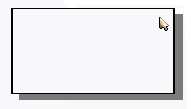
\includegraphics{Content/images/SystemInfo_1.png}
\caption{Basic WMAN Window}
\label{fig:FirstWindowInAction}
\end{figure}

You can see that so far, all we have defined is a small white window, with a shadow
and a black border. The pointer we are using is the default arrow and it is positioned
close to the top at the far right of the window. At least it works!

\begin{note}
You will not be able to assemble the code I have given you so far. There is a
lot more coding to do before you get to that stage. I have a test harness wrapped around
my window definition to make things easier for me to explain as I go along.
\end{note}

\subsection{Information Sub-{}Window List}
\label{ch23-info-windows}%hyperlabel{ch23-info-windows}%

Most PE programs that I have ever seen have a caption bar across the top, possibly
with a few loose items such as sleep (ZZz), Move and so on. The caption bar is usually -{}
but not always -{} green and white stripes with the program name displayed in the middle on
a white background. There are surprisingly, very few programs that do not stick to this
colour scheme, however, the new graphics drivers are changing this and we are starting to
get multi-{}coloured programs with trendy new 3D effects.

That sort of thing can wait until we get to grips with the basics, and so, in the
age old traditions of green and white stripes, we shall continue! In addition, the fancy
effects are only for those of us running SMSQ and so on, they are not available to the
128KB Standard Black Box QL users.

The usual method of getting the green and white caption bar is to define an
information sub-{}window that covers the required length of the window and position it at
the top of the window layout we are defining. The white background for the program name is
simply a second information sub-{}window positioned over the first one. Finally, the title
of the program itself is a text \emph{object} that the second (plain white)
information sub-{}window is linked to. 

To be accurate, the program title is a text string embedded within a text object
linked to the second information sub-{}window. All will become clear below.

The process could almost be likened to the following SuperBasic code.

\begin{lstlisting}[firstnumber=1,language={},caption={Pseudo SuperBasic Equivalent},label={lst:PseudoSuperBasicEquivalent}]
1000 REMark Main Window
1010 OPEN #3,con_
1020 WINDOW #3,160,84,50,32
1030 PAPER #3,7
1040 BORDER #3,1,0
1050 CLS #3
1060 :
1070 REMark Caption Bar background
1080 :
1090 WINDOW #3,98,14,50+30,32+0+1
1100 PAPER #3,85
1110 CLS #3
1120 :
1130 REMark Caption Bar White Bit
1140 :
1150 WINDOW #3,52,10,50+54,32+3+1
1160 PAPER #3,7
1170 INK #3,0
1180 CLS #3
1190 :
1200 REMark Program title
1210 :
1220 PRINT #3,' SysInfo'
1230 :
1240 CLOSE #3
\end{lstlisting}

It isn't quite the same as that, but things should hopefully become clear as we
progress. For now, the definitions of the information sub-{}windows is shown below and
should look strangely familiar.

\begin{lstlisting}[firstnumber=48,caption={WMAN Example Window - Information Window 0}]

; Information sub-window No. 0
infoList dc.w  98                   ; Sub-window width
         dc.w  14                   ; Sub-window height
         dc.w  30                   ; Sub-window x origin
         dc.w  0                    ; Sub-window y origin
         dc.b  $00                  ; MSbit clear to clear window
         dc.b  0                    ; Shadow depth 
         dc.w  0                    ; Border width 
         dc.w  0                    ; Border colour
         dc.w  85                   ; Paper colour (green/white)
         dc.w  0                    ; Pointer to info object list
\end{lstlisting}

Most of the above you have seen before in the fixed part of the main window
definition. As mentioned in the previous article, the shadow depth for sub-{}windows must be
zero. If you are like me, you'll be wondering what happens if you define a shadow on a
sub-{}window. It appears, nothing. I tried putting a shadow of size 1 on an information sub-{}
window and it simply was not drawn. I suspect that internally, WMAN\program{WMAN} is making as many
sanity checks as it can and is probably ignoring the shadow size.

The definition above is equivalent to lines 1070 to 1120 in the SuperBasic code
in Listing~\ref{lst:PseudoSuperBasicEquivalent}. That's an awful lot of typing for a simple result!

Next we need to define the second of our information sub-{}windows, the plain white
one used as a background for the title.

\begin{lstlisting}[firstnumber=last,caption={WMAN Example Window - Information Window 1}]

; Information sub-window No. 1
         dc.w  52                   ; Sub-window width
         dc.w  10                   ; Sub-window height
         dc.w  54                   ; Sub-window x origin
         dc.w  3                    ; Sub-window y origin
         dc.b  $00                  ; MSbit clear to clear window
         dc.b  0                    ; Shadow depth
         dc.w  0                    ; Border width 
         dc.w  0                    ; Border colour
         dc.w  7                    ; Paper colour (white)
         dc.w  infoObjs-*           ; Pointer to info object list

         dc.w  -1                   ; End flag
\end{lstlisting}

As this is our final information sub-window, there is a terminating word of -{}1 at the end of the
definition. The one thing to notice in these definitions is a pointer to a list of
information objects. These are explained next.

Setting the information objects list pointer to zero, in the above, and running the resulting
program gives us the window in \figurename~\ref{fig:FirstWindowInAction2}. You can see both of the information sub-{}windows
now, the green and white stripes is the first and the white one is the second. Next we
shall look at adding an information object to the second one.

\begin{figure}[h]
\center
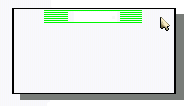
\includegraphics{Content/images/SystemInfo_2.png}
\caption{Basic WMAN Window - With Informations Windows}
\label{fig:FirstWindowInAction2}
\end{figure}


\subsubsection{Information Sub-{}Window Object List}
\label{ch23-info-objects}%hyperlabel{ch23-info-objects}%

There are 4 different types of object that you can place within an information sub-{}
window. These are shown in Table~\ref{tab:InfoSubWindowObjectTypes}.

\begin{table}[htbp]
\centering
\begin{tabular}{l l p{0.7\textwidth}}
\toprule
\textbf{Type} & \textbf{Code} & \textbf{Description} \\
\midrule
Text    &-N & This object is text. Character N will be underlined. \\
Text    & 0 & This object is text. There will be no characters underlined.\\
Sprite  & 2 & This object is a sprite.\\
Blob    & 4 & This object is a blob.\\
Pattern & 8 & This object is a pattern.\\
%
\bottomrule
\end{tabular}
\caption{Information Sub-Window Object Types}
\label{tab:InfoSubWindowObjectTypes}
\end{table}


If the type of the object is negative, then a text object is to be used and the
character in the string corresponding to the negative number `positivised' (I think I just
made up a new word!) will be underlined. We are not using that here, but when we come to
discuss Loose Items, we shall see an example or two.

The following is the definition of our text object for the program title.

\begin{lstlisting}[firstnumber=last,caption={WMAN Example Window - Information Object}]
infoObjs dc.w  42                   ; Object width
         dc.w  10                   ; Object height
         dc.w  6                    ; X origin
         dc.w  0                    ; Y origin
         dc.b  0                    ; Object type (See table)
         dc.b  0                    ; Spare
         dc.w  0                    ; Text ink colour
         dc.b  0                    ; Text character x size
         dc.b  0                    ; Text character y size
         dc.w  prgTitle-*           ; Pointer to object of correct type

         dc.w  -1                   ; end flag
\end{lstlisting}

As we only require one object for our information sub-{}window, there is the usual end
of list indicator word of -{}1 after the definition.

\begin{note}
The information in the following paragraphs has been added by George Gwilt since the original
article was published. These paragraphs correct the original one written by me.\footnote{In \emph{QL Today} Magazine}
\end{note}

If the object is text, the word at offset 10 gives the colour of the ink to be used to display the text. 

If the object is a blob (type 4) the word is used as a word relative pointer to the \emph{pattern} to be used with the blob.

If the object is a pattern (type 6) the word points to the \emph{blob} to be used with the
pattern. 

If the object is a sprite, the word is not used. In all cases the word at offset 14 points to the object itself
whether it is text, sprite, blob or pattern. Thus, for a sprite, its pointer is at offset 14, not 10 as Norman says.


Because this is a text object, we define the ink colour and the character sizes.
However, if the object type is non-{}text ie a blob, pattern or sprite, then the `ink' word
is used as a word sized relative pointer to a pattern or blob or sprite and the character
sizes are ignored. It may be wise to set those to zero just in case.

You will notice that the actual object content is defined elsewhere and one of those
word sized relative pointers (or zero!) is used to tell WMAN\program{WMAN} where the content can be
found.

Because our object is a text object, we simply define a QDSOMSQ format string as
normal and make sure our pointer above actually points to the string. The definition for
our program's title is as follows.

\begin{lstlisting}[firstnumber=last,caption={WMAN Example Window - Information Object Text}]
; Object No. 2       -> TEXT  
prgTitle dc.w  7
         dc.b  'SysInfo'
\end{lstlisting}

Now that we have defined all the required information sub-{}windows and objects that
are required for each, assembling my test program and running it gives the window in \figurename~\ref{fig:FirstWindowInAction3}.

\begin{figure}[h]
\center
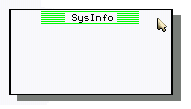
\includegraphics{Content/images/SystemInfo_3.png}
\caption{Basic WMAN Window - With an Information Object}
\label{fig:FirstWindowInAction3}
\end{figure}


Looks much better than the previous plain white version wouldn't you say? You can
see spaces along the caption bar and these will be used -{} very soon -{} for a couple of
loose items. Read on!

\subsection{Loose Item List}
\label{ch23-loose-items}%hyperlabel{ch23-loose-items}%

Loose items are probably the QL's equivalent of Windows Buttons. The following is
the definition of a loose item with a text object displayed upon it.

\begin{lstlisting}[firstnumber=last,caption={WMAN Example Window - Loose Item 0}]
;Loose menu item No. 1
         dc.w  24                   ; Width
         dc.w  11                   ; Height
         dc.w  132                  ; X origin
         dc.w  2                    ; Y origin
         dc.b  0                    ; Object x justification 
         dc.b  0                    ; Object y justification 
         dc.b  0                    ; Object type
         dc.b  3                    ; Selection keystroke
         dc.w  objESC-*             ; Pointer to object
         dc.w  1                    ; Loose item number
         dc.w  escape-*             ; Pointer to action routine
\end{lstlisting}

You can see a subtle difference between an information sub-{}window and a loose item
definition. Loose items have the properties listed in Table~\ref{tab:LooseItemProperties}.

\begin{table}[htbp]
\centering
\begin{tabular}{p{0.2\textwidth} p{0.7\textwidth}}
\toprule
\textbf{Property} & \textbf{Description} \\
\midrule
%
Hit area width            & The width of the loose item including the border width defined in the fixed definition \\
Hit area height           & The height of the loose item including the border width defined in the fixed definition \\
X origin                  & Where the loose iten will be drawn. Relative to the start of the layout \\
Y origin                  & Where the loose iten will be drawn. Relative to the start of the layout \\
X justification           & How the object will be positioned horozontally within the hit area \\
Y justification           & How the object will be positioned vertically within the hit area \\
Object type               & Same types and rules as for Information sub-window objects above \\
Selection Keystroke       & For a letter, the upper case letter. For an event it is the event number minus 14 \\
Pointer to object         & The usual word sized relative pointer to an object of the correct type. Zero if no text. \\
Loose item number         & The loose item number. You get to choose it. \\
Pointer to action routine & The address of the code to be called when this loose item is HIT or DOne \\
%
\bottomrule
\end{tabular}
\caption{Loose Item Properties}
\label{tab:LooseItemProperties}
\end{table}

As mentioned in Table~\ref{tab:LooseItemProperties}, objects are justified within the loose item hit
area. This is different from the positioning of objects in information sub-{}windows. Table~\ref{tab:LooseItemObjectJustificationRules} shows the justification settings.

\begin{table}[htbp]
\centering
\begin{tabular}{l p{0.7\textwidth}}
\toprule
\textbf{Code} & \textbf{Description} \\
\midrule
%
Positive & The object is left or top justified within the hit area \\
Zero     & The object will be centred within the hit area \\
Negative & The object is right or bottom justified within the hit area \\
%
\bottomrule
\end{tabular}
\caption{Loose Item Object Justification Rules}
\label{tab:LooseItemObjectJustificationRules}
\end{table}

If a key press is required to activate the loose item, it is defined by setting the
code of the capital letter to be used.

\begin{note}
More from George:

First of all, \emph{any} keypress including such things as TAB and the
arrow keys can be used. The selection is not confined to letters and those
keypresses which are defined as `events'. However, lower case letters are not
allowed.
\end{note}

If, on the other hand, some event is to be used to activate the loose item, then the
event number minus 14 is used instead. In our example above, the keystroke is set to 3 for ESC.

If you remember back to Chapter 21 when the event record was described, then you may
get an inkling of what the event number actually is. It is the bit set in the event vector
for the given action. Table~\ref{tab:EventsCodesDescriptions} shows the events and their details.

\begin{table}[htbp]
\centering
\begin{tabular}{l c c p{0.5\textwidth}}
\toprule
\textbf{Event Name} & \textbf{Event Number} & \textbf{Event Code} & \textbf{Description} \\
\midrule
%
DO     & 16 & 2 & ENTER pressed or right mouse button clicked \\
CANCEL & 17 & 3 & ESC pressed \\
HELP   & 18 & 4 & F1 pressed \\
MOVE   & 19 & 5 & CTRL+F4 pressed \\
RESIZE & 20 & 6 & CTRL+F3 pressed \\
SLEEP  & 21 & 7 & CTRL+F1 pressed \\
WAKE   & 22 & 8 & CTRL+F2 pressed \\
%
\bottomrule
\end{tabular}
\caption{Events, Codes and Descriptions}
\label{tab:EventsCodesDescriptions}
\end{table}


\begin{note}
More updates by George.

The official documentation refers to "event number" and "event code". The event number is the number of the bit
set in the event vector which is at position \$14 in the window status area. For the seven events listed by Norman the
corresponding bits to be set are 16 to 22. The event code is the event number less 14. 

If a loose item is to be activated by a keypress producing an event the selection keystroke must be the event
code as Norman says.
\end{note}

The action routine is called when the loose item is HIT or DOne. The parameters
passed to the action routine will be discussed in a later article.

\subsubsection{Loose Item Object List}
\label{ch23-loose-objects}%hyperlabel{ch23-loose-objects}%

Loose item objects are identical to those for information sub-{}windows and so, are
the same to define. The following is an example of the text object required by our example
loose item above.

\begin{lstlisting}[firstnumber=last,caption={WMAN Example Window - Loose Item Object Text}]
; Object No. 4       -> TEXT  
objESC   dc.w  3
         dc.b  'ESC'
\end{lstlisting}

Nothing at all surprising there, it is a text object after all and as such, we
simply define a QDOSMSQ string in the normal manner. Had the object been a blob, pattern
or sprite, we would define one of those in the normal manner. More on those objects later
on in the series.

Now that we have defined all the required loose items and objects that are required
for each, assembling my test program and running it gives the following. I have moved the
pointer from its default position in the screenshot in \figurename~\ref{fig:FirstWindowInAction4} so that you can see the contents of
all the loose items without obstruction.

\begin{figure}[h]
\center
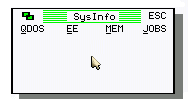
\includegraphics{Content/images/SystemInfo_4.png}
\caption{Basic WMAN Window - With Loose Items}
\label{fig:FirstWindowInAction4}
\end{figure}

All we need now is an application sub-{}window for our code to write to and we are
ready to add actions etc. I shall keep you in suspense until next time.

\section{Coming Up...}
\label{ch23-the-end}%hyperlabel{ch23-the-end}%

In the next chapter we shall continue looking at the remainder of the
standard window definition. It seems like there is quite a lot going on, but it will
hopefully soon be quite easily understood.

We will take a look at adding simple application sub-{}windows and
creating loose item action routines. We might even get a working program to play with, who
knows? See you then.




\part{SETW and Easy PEasy}

\chapterimage{chapter_head_1.pdf} % Chapter heading image
\chapter{Creating Your Own Windows With SETW}
\program{SETW}

\label{ch24}%hyperlabel{ch24}%

\section{Introduction}
\label{ch24-intro}%hyperlabel{ch24-intro}%

In this chapter, I shall be taking a small diversion into one
        of George Gwilt's utility programs. This one, SETW\program{SETW}, allows you to interactively
        create windows for your applications. SETW\program{SETW} then goes away and does all the hard
        work of setting everything up.

\section{Downloading SETW}
\label{ch24-setw}%hyperlabel{ch24-setw}%

SETW\program{SETW}, and other useful utilities, are available from George's web site, \url{http://gwiltprogs.info/} and from there I advise you to download the following three utilities:
\begin{itemize}[itemsep=0pt]

\item{}SETW -{} setwp05.zip


\item{}EasyPEasy -{} peassp02.zip


\item{}GWASL -{} gwaslp07.zip

\end{itemize}

The latest version of GWASL\program{Gwasl} is required to enable you to assemble PE
        programs created using SETW\program{SETW} and using the EasyPEasy\program{EasyPEasy} library files in peassp02.zip.
        As you will require these for the remainder of the tutorial then you should
        download them all now to save time later.

There are other files there similarly names but with a `p' replaced by and
        `s' -{} these are the sources for the utilities and while educational, you don't
        need them.

The files are zipped up using the QDOS version of zip, so copy them from
        wherever you downloaded them to into your QL system (QPC etc) and unzip them using
        the QDOS version of unzip. There is one supplied with the C68\program{C68} system and that
        works fine.

\section{Running SETW}

In order to create correctly written assembly source for GWASL\program{Gwasl}, we need to
        pass a single parameter to SETW\program{SETW} when we execute it. The parameter is "-{}abin" with
        no spaces. This tells SETW\program{SETW} that the code produced will be used to build a binary
        file rather than a relocatable one which will be subsequently linked with other
        relocatable files to produce the final binary.

We GWASL\program{Gwasl} users don't have a linker so all our programs need to be self
        contained, or may include pre-{}assembled modules and libraries using the LIB
        command.

\begin{lstlisting}[firstnumber=1,caption={Executing SETW},language={}]
EX SETW ; '-abin'
\end{lstlisting}

The command above is all we need. If you do not have Toolkit 2, then the
        EXECUTE command from Turbo Toolkit can be used instead.

We will use SETW\program{SETW} to create a file that we will use later on. It will be a
        very simple window with a single information window near the top and a single text
        object within the information window. Feel free to follow along on your own QL
        system as we go.

The program starts by opening a window as big as it can on your screen, it
        displays a few bits of information and prompts for the root name of the various
        files to be created.

For our example, we simply set the name to `hello' -{} without the quotes.
        Type it in and press ENTER.

SETW\program{SETW} will create three files when we are done. They will be created on ram1\_
        (in my case) or wherever you have configured SETW\program{SETW} to put them by default. The
        three files created will be:
\begin{itemize}[itemsep=0pt]

\item{}Ram1\_hello\_wda -{} a file for use by George's TurboPTR\program{TurboPTR} utility. It is
                of no use to us and can be safely deleted when finished.


\item{}Ram1\_hello\_asm -{} a file for use by an assembler, in our case, GWASL\program{Gwasl},
                this is the file we will need.


\item{}Ram1\_hello\_z -{} a file for use with another of George's utilities,
                CPTR\program{Cptr}, a program to help C68\program{C68} users write PE programs. Again, we don't need
                this file and it can safely be deleted.

\end{itemize}

\subsection{Entering Text Objects}

The next screen that appears is titled `ALTER TEXT' and is where we
            enter every text object to be used in our finished utility. We must be very
            careful here and not forget any because SETW\program{SETW} creates code for what we enter
            and we cannot go back and add another if we forget one. (Well possibly we can
            in the generated assembler file, but I have not confirmed this yet.)

To enter your text objects, press the `N' key to create a new text
            object and simply type in the required text. For our example window all we
            need is one single object containing the text `Hello World' (without quotes) -{}
            for the main reason that this is how everyone starts to learn a new language!
            Press ENTER when you have entered the text.

In slightly more complicated programs, there would be a lot more text
            objects to enter, but for now, press the ESC key to exit from the ALTER TEXT
            screen.

\subsection{Entering Sprites, Blobs \& Patterns}

We don't need any sprites, blobs or patterns in this example, so simply
            press the ESC key when prompted for each of these.

\subsection{The Main Window}

The next prompt is to tell SETW\program{SETW} about the main window, how many windows
            are needed and so on. In many cases the default is correct and all we need do
            is press ENTER at each prompt -{} however, make sure you read the prompt and
            think before pressing ENTER -{} once you have done so, there's no going back!
            (Ask me how I know!)

When asked for the number of main windows, accept the default of 1 by
            pressing ENTER.

When asked for the number of loose Items, accept the default of zero by
            pressing ENTER.

When asked for the number of Information Windows, we will need one, so
            press the `1' key and press ENTER.

We are now asked to enter the number of information objects in each
            information window. We require one information object in our one single
            information window. Type `1' and press ENTER.

When asked how many Applications Windows you want, accept the default of
            zero.

Next we are asked to select a shadow size. I find a size of 2 to be
            adequate. Type `2' and press ENTER.

For the border size choose a width of 1.

For all the prompts asking us to select a colour, select option 1 each
            time. Use the arrow keys to highlight the desired option and press ENTER to
            select it. We want "1. Default" for our colours. (I will explain the others
            later on in the series.)

Next we get to choose the sprite to be used as a pointer in the main
            window. I much prefer the standard arrow, so select it as above, and press
            ENTER. If you wish, you can choose another sprite to use as the pointer
            instead -{} it's your choice.

\subsection{Information Windows \& Objects}

Now that all the details for the main window have been entered, or
            default chosen, we get to enter the requirements for each (or in our case,
            one!) Information Window.

First of all we need to enter the border width, I use a width of one
            pixel for all my programs. Type `1' and press ENTER.

Next we need the border colour, as before, select "1. Default" and press
            ENTER.

Select the default again for the paper colour.

We are now asked to select a type for our information objects for this
            information Window. As we only entered a single information object way back at
            the beginning and that was a text object, we should select "text" and press
            ENTER. Other object types would be available if we had entered any sprites,
            blobs or patterns.

Next we see a window appear with the list of (one!) text objects. As
            there is only one, it has been highlighted for us. Press ENTER to select
            it.

Select the default colour again.

When asked for the character sizes for X and Y for this text object,
            select zero for both.

\subsection{Interactively Sizing The Window \& Contents}

Now the fun begins! A window appears that allows us to interactively
            resize the main window and the information window we have created. Once done,
            we can position these items almost at will.

Looking at the window currently being displayed, the lower right corner
            shows the currently defined dimensions for the main window itself. At the top
            left is an outline of the noted dimensions. We can use the arrow keys to
            change the dimensions -{} up makes the window less tall, down makes it taller,
            left makes the window narrower and right makes it wider.

Pressing the ALT key makes the change in size bigger. This saves wearing
            out your keyboard getting the window to the size you would like!

For this demonstration program, we require a window size of 200 wide by
            100 deep. Use the ALT and arrow keys to make the dimensions 200 wide and 100
            deep. When the desired dimensions have been achieved, press ENTER.

We are now asked if a variable window is to be created, this will be
            covered in a future tutorial so for now, type `N'. (There is no need to press
            ENTER.)

Next we need to set the origin of the window. Again the arrow keys move
            things around and the ALT key makes the movements bigger. For the
            demonstration, set the origin to 50, 50. You will get a rough idea of where
            the origin will be as a small dot moves around the screen under the control of
            your arrow keys. Press ENTER when the origin is where you would like it to
            be.

Next up, we get to size our information windows, or window in our case!
            I have decided to make it slightly wider than the space required for the text
            object. That itself is 12 characters of 6 pixels wide or 72 pixels in total.
            As I like to have a bit of leading and trailing space in my information
            windows, use the arrow keys and ALT, as before, to resize information window
            number one to be 74 pixels wide by 12 deep. You may choose a different
            dimension if you like, but it will need to be a minimum of 72 pixels wide to
            hold all the text.

The program starts off in position mode rather than in size mode. You
            may need to press F2 to toggle between the two modes. Check the prompt on
            screen for advice about which mode you are currently in.

Once you have the desired size, press F2 and move the window to a
            position of 62 across by 2 down. If the information window size plus the
            position causes it to extend off the edge(s) of the main window, you will not
            be allowed to position it where you want to. In this case, toggle between size
            and position with the F2 key until you have it correctly sized and
            positioned.

Press ENTER when done. This takes you now to the sizing and positioning
            of the information window object (where the actual text object will be
            placed). If you remember the text object is 12 characters or 72 pixels wide
            which means that we need an object big enough to take that plus a little space
            at the beginning and end. As I like a couple of pixels either end of my
            objects, set the information object to be at position 4 across and 1 down.
            Press ENTER when satisfied.

That's it for our little test window. SETW\program{SETW} now displays some information
            about the files it created and after a pause, or when you press a key, it will
            cycle through all the main windows we created -{} one in our case -{} and display
            them on screen as they have been defined.

At this point, there's not much we can do if it all went horribly wrong.
            We simply have to start again -{} or get down and dirty in the generated
            assembly file! Press ENTER to exit from SETW.

On ram1\_, in my case, we now have the files that SETW\program{SETW} generated for us.
            We are only interested in the hello\_asm file and can happily delete the
            others. Feel free to examine the generated file in an editor and compare what
            has been created with the previous articles where I explain what the
            individual bits of a WMAN\program{WMAN} window definition are.

The assembly source file generated is not able to be assembled as it is
            and then run, it has no code in it to make it a correctly functioning QDOS
            job. That comes later.

Until next time, feel free to generate more windows of your own and get
            to know George's SETW\program{SETW} utility -{} we will be using it in future articles in this
            series.

\section{Coming Up...}
\label{ch24-the-end}%hyperlabel{ch24-the-end}%

We take the file we created with SETW\program{SETW} and feed it into
        another of George's utilities, EasyPEasy, in the next chapter. EasyPeasy tries to make coding for the PE
        much easier. Until next time, happy windowing.



\chapterimage{chapter_head_2.pdf} % Chapter heading image
\chapter{Easy PEasy -{} Part 1.}

\section{Introduction.}
\label{ch25-intro}%hyperlabel{ch25-intro}%

At the end of the previous chapter, we had created a very minimal `Hello
    World' window using George Gwilt's SETW\program{SETW} application. In this chapter, we
    take a first look at George's other utility to make PE programming easy,
    EasyPEasy\program{EasyPEasy}. As mentioned last time, you should have downloaded the
 peasp02.zip file from George's website. If you find a
    later version (say peasp03.zip or higher, get that
    instead!) The website address is \url{http://gwiltprogs.info/}.

\section{Easy PEasy.}
\program{EasyPEasy}
\label{ch25-std-windef-cntd}%hyperlabel{ch25-std-windef-cntd}%

Unlike many other utilities, Easy PEasy\program{EasyPEasy} isn't a program you can run,
    it is a collection of information and small binary files that you can
    include with your own programs -{} using the LIB and IN commands in your
    source code and assembling with GWASL\program{Gwasl} -{} to make programming the Pointer
    Environment a little easier. Actually, quite a lot easier as George has
    done much of the hard work, all we have to do is open a console, make a
    few checks and write the code to handle our own needs as opposed to the
    needs of getting the PE up and running.

Much of what follows in this chapter is a blatant theft of George's
    readme file. For this I make no apology -{} there is no better way to
    document something that straight from the horse's mouth!

\section{The Nine Steps To Happiness.}

With Easy PEasy\program{EasyPEasy}, there are nine steps to happiness. The following is
    basically a skeleton for writing a PE program in assembly language:

\begin{enumerate}[itemsep=0pt]

\item{}Initialise your program and open a con\_ channel.

\item{}Are the PTR\_GEN\program{PTR\_GEN} \& WMAN\program{WMAN} present? Abort the program if not.

\item{}Set up the window working definition.

\item{}Position the window.

\item{}Draw the window contents.

\item{}Read the pointer.

\item{}Did we have an error -{} exit if so, else it was an event.

\item{}Process the event.

\item{}Goto step 6.

\end{enumerate}

Each step in the above, thanks to the coding that George has done,
    is quite simple.

\subsection{Initialise.}

The initialisation step consists of setting up your console
      channel and opening it. The standard QDOSMSQ job header is also
      required. The code is very simple, and looks like that shown in \lstlistingname~\ref{lst:EasyPEasy-1}. It
      is best to do the setup as soon as possible after the program is
      executed rather than setting up other stuff first. It saves time and
      effort -{} in case something goes wrong and you have to bale out.

\begin{lstlisting}[firstnumber=1,caption={EasyPEasy Standard Code - Initialisation},label={lst:EasyPEasy-1}]
        bra.s     start
        dc.l      0
        dc.w      $4afb

id      equ       0                 ; Storage for channel id
wmvec   equ       4                 ; Storage for WMAN vector
slimit  equ       8                 ; Storage for Window limits call

jname   dc.w      jname_e-jname-2
        dc.b      "My EPE Program"
jname_e ds.b      0
        ds.w      0

; Console definition.
con     dc.w      4
        dc.b      'con_'

; The job starts here.
start   lea       (a6,a4.l),a6      ; Get the dataspace address in A6.L

        lea       con,a0            ; Con_ channel definition
        moveq     #-1,d1            ; Required for this job
        moveq     #0,d3                          
        moveq     #io_open,d0
        trap      #2                ; Open the channel
        tst.l     do                ; Did it work?
        bne       sui               ; Exit via sui routine in EasyPEasy
        move.l    a0,id(a6)         ; Save the channel id
\end{lstlisting}

\subsection{Check The PE \& WMAN.}

The console is open now, or we have baled out of the program.
      Obviously we don't get much feedback from the program if anything went
      wrong, a proper user friendly application would, of course, display a
      suitable error message. The next easy step is to check for the presence
      or otherwise of PTR\_GEN\program{PTR\_GEN} and WMAN\program{WMAN} as per \lstlistingname~\ref{lst:EasyPEasy-2}.

The following code requires a channel id, for a CON\_ channel, to
      be in A0.

\begin{lstlisting}[firstnumber=last,caption={EasyPEasy Standard Code - Checking for the PE},label={lst:EasyPEasy-2}]
; Check for PE being present.
        moveq     #iop_pinf,d0
        moveq     #-1,d3
        trap      #3
        tst.l     d0                ; Ptr_gen present?
        bne       sui               ; No, bale out
        move.l    a1,wmvec(a6)      ; Yes, save WMAN vector
        beq       sui               ; Oops! Bale out, no WMAN
        movea.l   a1,a2             ; Keep WM vector in A2
        lea       slimit(a6),a1     ; Storage, 4 words long
        moveq     #iop_flim,d0      ; Need maximum size of window
        trap      #3
        subi.l    #$C0008,(a1)      ; Less 12 (width) and 8 (height)
\end{lstlisting}

The code in \lstlistingname~\ref{lst:EasyPEasy-2} checks for the PE being present and if not found,
      bales out via the code at sui. If the PE is found, the WMAN\program{WMAN} vector is
      saved in data space for later use -{} however, if WMAN\program{WMAN} is not loaded (but
      PTR\_GEN\program{PTR\_GEN} is) the job will exit via the familiar sui routine. Easy PEasy\program{EasyPEasy}
      requires both the PTR\_GEN\program{PTR\_GEN} and WMAN\program{WMAN} files to be loaded in order to
      create and run PE programs.

Next up, we find out the maximum size that the con\_ channel can
      grow to. We assume that that code always works -{} but it may be good
      practice to check, just in case. The 4 words returned indicate the size
      and position of the con\_ channel, and these 4 words are placed into the
      job's data space and a small margin is subtracted from the width and
      height.

\subsection{Set The Window Definition.}

The window definition is expected to hold a value in wd0 for the
      size of working definition and status area space. The code in \lstlistingname~\ref{lst:EasyPEasy-3} reads
      the amount of memory required for the window definition (created by SETW\program{SETW}
      and defined in ww0\_0) and allocates space in the common heap for our
      program to use. If this fails, the call to getsp will never return -{} it
      exits through the sui code on error.

\begin{lstlisting}[firstnumber=last,caption={EasyPEasy Standard Code - Allocate Memory for the Window Definition},label={lst:EasyPEasy-3}]
; Reserve memory for the window working definition.
        lea       wd0,a3           ; Address of window definition
        move.l    #ww0_0,d1        ; Size of working definition
        bsr       getsp            ; Allocate space
        movea.l   a0,a4            ; Save in A4.L too
\end{lstlisting}

If the memory allocation worked, the address is returned in A0 and
      we save it in A4 for later use. This is a handy feature of Easy PEasy\program{EasyPEasy}
      and the way it was written by George.

Before we can call the WMAN\program{WMAN} routine to set up our window -{}
      \pe{wm\_setup} -{} we need to make sure that the status area for loose items is
      all initialised properly. The code in \lstlistingname~\ref{lst:EasyPEasy-4} assumes that all loose
      items will be available when the program starts. Zero is the value we
      need for available.

The labels wst0 and wst0\_e are defined by the SETW\program{SETW} program. (As
      you can see SETW\program{SETW} does most of the hard work of calculating various sizes
      and labels for us!)

\begin{lstlisting}[firstnumber=last,caption={EasyPEasy Standard Code - Loose Item Initialisation},label={lst:EasyPEasy-4}]
; Preset all Loose Items to available.
         movea.l   id(a6),a0       ; Restore channel ID
         moveq     #wst0_e-wst0-1,d1 ; Size of status area - 1
         lea       wst0,a1         ; Wst0 = status area address

loop     clr.b     (a1)+           ; Zero = Loose Item is available
         dbf       d1,loop         ; Clear entire area
         lea       wst0,a1         ; Reset pointer to status area
         moveq     #0,d1           ; Default window size
         lea       wd0,a3          ; Wd0 = window definition address
         jsr       wm_setup(a2)    ; Create the working definition
\end{lstlisting}

\subsection{Position The Window.}

This is probably one of the easiest parts of the code! We assume
      that the pointer is in the position on screen where we wish the window
      to appear. The position of the window may move to make sure that it
      remains on the screen, however, in normal circumstances, the pointer in
      our window will be positions in exactly the same place where the on
      screen pointer is now.

\begin{note}
If you don't default the pointer position to -{}1 to indicate
        where the pointer is now, then you must note that the value in D1 is
        in absolute screen coordinates relative to the start of the screen (at
        0,0) and not relative to the program's main window or to any
        application sub-{}windows within.
\end{note}

This can be useful if a window has no `move' abilities -{} you can
      simply put the pointer where you wish the window to appear, and execute
      the program. The window will be drawn exactly (adjusted to fit on
      screen) where you have put the pointer.

\begin{lstlisting}[firstnumber=last,caption={EasyPEasy Standard Code - Position the Window},label={lst:EasyPEasy-5}]
; Position, but do not draw, the window.
         moveq     #-1,d1          ; Position at pointer position
         jsr       wm_prpos(a2)    ; It's a primary window
\end{lstlisting}

\subsection{Draw The Contents.}

The windows has been positioned, however, it has not been drawn on
      screen, so we need to draw it now. This is even simpler than the
      positioning of the windows.

\begin{lstlisting}[firstnumber=last,caption={EasyPEasy Standard Code - Draw the Window},label={lst:EasyPEasy-6}]
; Draw the window.
         jsr       wm_draw(a2)     ; Draw the window and its contents
\end{lstlisting}

That was difficult! ;-{})

\subsection{The Pointer Loop.}

At this point, we have the windows on screen and the user is
      waiting to use the application. We have to enter a loop to read the
      pointer and act accordingly.

\begin{lstlisting}[firstnumber=last,caption={EasyPEasy Standard Code - Reading the Pointer},label={lst:EasyPEasy-7}]
; Main pointer reading loop.
read_ptr jsr       wm_rptr(a2)     ; Read the pointer. 
;                                  ; Does not return until
;                                  ; Either D0 or D4 are non-zero
\end{lstlisting}

For most loose items, application windows and so on, an action
      routine will have been defined and coded. These action routines will be
      discussed later. The pointer reading routine -{} \pe{wm\_rptr} -{} will not return
      until either D0 or D4 are non-{}zero as a result of an action
      routine.

\subsection{Error Or Event?}

If D0 is non-{}zero, and error has occurred and we should (somehow)
      handle it and probably bale out of the program. Alternatively, we can
      simply ignore errors and try again. The program developer
      decides.

If D4 is non-{}zero, an event has occurred and we need to handle
      that in our code before, possibly, returning to the pointer reading loop
      again.

An event is defined as a key press such as ENTER while the pointer
      is not positioned on a loose item or menu item, ESC, F1 (Help) or any of
      the CTRL+Fn key combinations -{} SLEEP, WAKE, MOVE or SIZE -{} but only
      provided that the key press doesn't select a menu item.

An event can be generated by any of the action routines as well.
      Within the action routines the programmer has the choice of either
      handling the action code there and then, or, setting an event in D4 and
      returning. This will cause the call to \pe{wm\_rptr} to exit and return back
      to the application where the event can be handled.

Some programmers like to control where and when the action
      handling code is performed and like to keep it all in the main code,
      others like to carry out the actions within the action handlers. It's
      entirely up to the developer -{} the end user will see no difference
      whichever method is chosen.

Obviously, how a program handles errors and events is up to the
      programmer and a generic method can't be given here. However, as an
      example, the following may suffice.
\begin{lstlisting}[firstnumber=last,caption={EasyPEasy Standard Code - Error or Event Check},label={lst:EasyPEasy-8}]
; Ignore errors.
         bne.s     read_ptr        ; Error in D0? If so, ignore it
;                                  ; This assumes there is an option in
;                                  ; the program to let the user EXIT
\end{lstlisting}


\subsection{Process Events.}

At this stage in our program, we have returned from reading the
      pointer (\pe{wm\_rptr}) and no errors have been reported (in D0), so we must
      have detected an event in D4. We have three choices here -{} if our action
      routines should have handled things, then perhaps we should ignore the
      event and read the pointer again -{} alternatively, this could be an error
      and we should abort the program. The other alternative is that our
      action routines have set the event in D4, so our code should now process
      the appropriate event.

As above when trapping errors, there's no `one size fits all'
      answer and every program should handle events accordingly. The following
      is an example whereby the events are simply ignored and we return to
      reading the pointer.

\begin{lstlisting}[firstnumber=last,caption={EasyPEasy Standard Code - Ignore Events},label={lst:EasyPEasy-9}]
; Ignore events.
         bra.s     read_ptr        ; Ignore event numbers in D4
\end{lstlisting}

Obviously, if your code is processing events `outside the action
      routines' then your own code, to process the appropriate event, would go
      here, rather than simply ignoring the events.

The event numbers are discussed below in `Loose Item Action
      Routines'.

\subsection{Repeat.}

Repeat has already been handled above. All we do -{} in this simple
      example -{} is loop back to read the pointer when we hit an error or when
      any event occurs.

\section{Loose Item Action Routines.}

There are two kinds of action routines you need to be aware of.
    Those for loose items and those for application menu items. As we have not
    yet discussed much for Application Windows or their menu items, they will
    be discussed later.

An action routine for a loose item is called from within the \pe{wm\_rptr}
    call, and if the action routine exits with D0 and D4 both set to zero, the
    \pe{wm\_rptr} call will resume again -{} in other words, control will not return
    to your own code just yet.

On entry to a loose item action routine various registers are set
    with specific parameters:


\begin{table}[htbp]
\centering
\begin{tabular}{l p{0.8\textwidth}}
\toprule
\textbf{Register} & \textbf{Description}  \\
\midrule
%
D1.L & High word = pointer X position, Low Word = pointer Y position.  \\
D2.W & Selection keystroke letter, in its \emph{upper cased} format, or 1 = Hit/SPACE or 2 = DO/ENTER.  D2.W may be an \emph{event code} if an event triggered this action.  \\
D4.B & An event number - see below - if an event triggered this action routine.  \\
A0.L & Channel id.  \\
A1.L & Pointer to the status area.  \\
A2.L & WMAN vector.  \\
A3.L & Pointer to loose menu item.  \\
A4.L & Pointer to window working definition.  \\
%
\bottomrule
\end{tabular}
\caption{Loose Item Action Routine - Entry Registers}
\label{tab:Loose ItemActionRoutineEntryRegisters}
\end{table}

If the loose item was triggered as the result of a selection
    keystroke, D2.W will hold the uppercased letter code.

If the loose item was triggered as a result of an event, D4.B holds
    the \emph{event number} and D2.W holds the \emph{event
    code} in the table below.


\begin{table}[htbp]
\centering
\begin{tabular}{l l c c}
\toprule
\textbf{Event} & \textbf{Keystroke} & \textbf{Event Number (D4.B)} & \textbf{Event Code (D2.W)}  \\
\midrule
%
Hit    & Space    &  0 & 1 \\
Do     & Enter    & 16 & 2 \\
Cancel & ESC      & 17 & 3 \\
Help   & F1       & 18 & 4 \\
Move   & CTRL+F4  & 19 & 5 \\
Size   & CTRL+F3  & 20 & 6 \\
Sleep  & CTRL+F1  & 21 & 7 \\
Wake   & CTRL+F2  & 22 & 8 \\
%
\bottomrule
\end{tabular}
\caption{Loose Item Action Routine - Event Settings}
\label{tab:Loose ItemActionRoutineEventSettings}
\end{table}

In addition to the above, the status of the loose item which
    triggered the action routine will be set to selected. It is not reset to
    available on exit, this is your responsibility.

Action routines must exit with D5, D6 and D7, A0 and A4 preserved to
    the same value that they had on entry to the routine. In addition, the
    code must set the SR according to the value in D0. A5 and A6 can be used
    and left at any value by the action routines, while D1 -{} D3 and A1 -{} A3
    appear to be undefined as to their exit status.

If an error is detected, the routine should exit with an error code
    in D0 and the SR set accordingly. If the action routine simply wishes to
    cause \pe{wm\_rptr} to return to the user's code where an event will be
    processed -{} rather than processing it in the action routine itself, D4
    should be set to the correct event number that the user code should
    process.

Obviously, if setting D4 with an event number then D4 should be set
    before D0 otherwise the SR will take on the settings for D4 instead of
    D0.

If no error was detected by the action routine, and no event is to
    be returned, both D0 and D4 must be set to zero on exit.

The action routine needs to perform the application specific code to
    process the loose item that was triggered, however, it must also reset the
    status of the loose item that triggered the action routine. This can be
    done as follows.

\begin{lstlisting}[firstnumber=last,caption={EasyPEasy Standard Code - Actions},label={lst:EasyPEasy-10}]
; Action routine code goes here ...
         move.l    d5-d7/a0-a4,-(a7) ; Preserve registers that we need
         ...                         ; Do your stuff!
         move.l    (a7)+,d5-d7/a0-a4 ; Restore registers prior to exit
      
; Reset loose item status as part of action routine.
         move.w    wwl_item(a3),d1 ; Get the loose item number
         move.b    #wsi_mkav,ws_litem(a1,d1.w) ; Redraw as available
         moveq     #-1,d3          ; Request a selective redraw
         jsr       wm_ldraw(a2)    ; Redraw selected lose items
         moveq     #0,d4           ; No event signalled here
         moveq     #0,d0           ; No errors either
         rts                       ; Back to wm_rptr
\end{lstlisting}

The code above could be used as a template for loose item action
    routines. It begins by preserving the registers that we must preserve
    plus, it stacks A1 and A2 as well -{} for added safety, as they will be
    required in the code to reset the loose item status.

Should you reset the status on entry to the routine or exit? It's up
    to your code obviously. However, I prefer to do it at the end of the
    action routine. If the action routine is short and quick, it probably
    makes no difference. If the routine takes some time -{} lets say, it's
    formatting a floppy disc -{} then it's best to leave it at selected until
    the format finishes and then reset it. However, it's your choice.

\section{Coming Up...}

In the upcoming chapter, we'll take a deeper look at
    Easy PEasy\program{EasyPEasy} and the routines that George has written for us. If we have
    time and space, we might take a look at an example of its use. See you
    then.



\chapterimage{chapter_head_1.pdf} % Chapter heading image
\chapter{Easy PEasy -{} Part 2.}

\section{Introduction.}
\label{ch26-intro}%hyperlabel{ch26-intro}%

At the end of the previous chapter -{} Easy PEasy\program{EasyPEasy} Part 1, I promised to take a look
        at the various code routines that George has written to make life a lot easier for
        PE assembly language programmers. If you haven't already done so, get over to
        George's web site and download the programs mentioned last time. The website
        address is \url{http://gwiltprogs.info/}.

\section{Easy PEasy.}
\label{ch26-easy-peasy}%hyperlabel{ch26-easy-peasy}%

As I mentioned last time, Easy PEasy\program{EasyPEasy} isn't a program you can run, it is a
        collection of information and small binary files that you can include with your
        own programs -{} using the LIB and IN commands in your source code and assembling
        with GWASL\program{Gwasl} -{} to make programming the Pointer
        Environment a little easier.

\section{Supplied Files.}
\label{ch26-files-supplied}%hyperlabel{ch26-files-supplied}%

With Easy PEasy\program{EasyPEasy}, there are a number of files supplied, these are:

{\bf Keys\_pe} 
A file that can be included in your source file to define a number of
            equates for the various Trap \#3 routines introduced by the PE.

{\bf Keys\_wdef} 
Another include file. This one defines the WMAN\program{WMAN} window definition
            equates.

{\bf Keys\_wman} 
Similar to keys\_pe above but this file defines the
            equates for WMAN\program{WMAN} routines and vectors.

{\bf Keys\_wstatus} 
This file defines the equates etc for the window status area.

{\bf Keys\_wwork} 
This file contains the definitions for the window working
            definition.

{\bf Qdos\_pt} 
The equates etc for the PE interface.

{\bf Csprc\_bin} 
Some sprites, mostly for mode 4 but a few exist for mode 8. This file
            should be LIBbed by your own programs to use the sprites.

{\bf Csprc\_sym\_lst} 
This file lists the names of all the sprites in the above file. If you
            need to use a sprite in the above (binary) file, you must use the name listed
            in this file.

{\bf Peas\_bin} 
This file contains all the useful code subroutines that George has
            written to make using the PE from assembly language easy. This file is binary
            and as such, should be LIBbed by your source code.

{\bf Peas\_sym\_lst} 
This file lists all the routines supplied in the above file. Make sure
            that you use the name(s) listed in this file if you wish to use George's code
            in your own PE programs.


\section{Subroutines in Easy PEasy.}
\label{ch26-sub-routines}%hyperlabel{ch26-sub-routines}%

The file peas\_bin should be included at the very end of your
        own program's code, as follows:

\begin{lstlisting}[firstnumber=1,caption={Invoking EasyPEasy in Your Own Programs}]
         in        win1_source_easypeasy_peas_sym_lst
         lib       win1_source_easypeasy_peas_bin
\end{lstlisting}

The first `in' line includes the peas\_sym\_lst file
        which defines offsets from the current position to the entry points for the
        routines in the peas\_bin file which is copied `as is'
        straight into your final executable file. For this reason, you must keep these
        lines together and in the order shown above.


\begin{table}[htbp]
\centering
\begin{tabular}{l p{0.8\textwidth}}
\toprule
\textbf{Routine} & \textbf{Description}  \\
\midrule
%
GetSp & Allocates an area of memory and returns the address in A0.L. The size of the area required must be passed in D1.L on entry. No other registers are affected. Exits via SUI (see below) if the memory allocation causes an error.\\
Rechp & Deallocates and frees an area of memory allocated by GetSp above. The address should be passed in A4.L. No other registers are affected.\\
Move & Processes a MOVE request then returns with D4 and D0 both set to zero. No other registers are affected. Can be called from inside the MOVE action routine in your own programs.\\
Sleep & Puts the program to sleep and creates a button in the button frame - if present. If the button frame is not present, the button will be placed on the top left of the display. See below for register usage.\\
Set\_AP & Set an application window menu. See below for register usage. All registers are preserved on exit.\\
Sui & The program exits without warning and without any error messages. GetSp above will exit through here if there is an error when allocating memory.\\
%
\bottomrule
\end{tabular}
\caption{EasyPEasy Library Routines}
\label{tab:EasyPEasyLibraryRoutines}
\end{table}

\subsection{GetSp}
\label{ch26-sub-getsp}%hyperlabel{ch26-sub-getsp}%

GetSp allocates an area of memory for the current job, and returns the
            address in register A0.L. There are no errors returned (in D0) as the routine
            exits through sui (below) if it detects an error. Only register A0.L is
            affected by the routine -{} all others are preserved.

On entry, the number of bytes required should be held in D1.L. On exit,
            A0.L holds the address of the allocated area. An example of use, taken from
            George's example EX0\_asm, can be see in \lstlistingname~\ref{lst:EasyPeasyGetSPExample}.

\begin{lstlisting}[firstnumber=1,caption={EasyPEasy - GetSP Example},label={lst:EasyPeasyGetSPExample}]
         ...
         move.l    #ww0_0,d1      ; Size of working definition.
         bsr       getsp          ; Return ALCHP'd address in A0.
         movea.l   a0,a4          ; Copy to A4.
         ...
\end{lstlisting}

There is no requirement to check for an error with this routine, if it
            returns to your program then it has worked.

\subsection{Rechp}
\label{ch26-sub-rechp}%hyperlabel{ch26-sub-rechp}%

Rechp returns an area of memory, probably allocated using GetSp above,
            to the system. The address to deallocate must be passed in A4.L. All other
            registers are preserved and no errors are returned by this routine. An example
            of use would be after unsetting a widow definition, as per the following from
 EX0\_asm:

\begin{lstlisting}[firstnumber=1,caption={EasyPEasy - Rechp Example},label={lst:EasyPeasyRechpExample}]
         ...
         jsr       wm_unset(a2)
         bsr       rechp
         ...
\end{lstlisting}

Again, there is no need to check for errors as the routine never
            fails.

\subsection{Move}
\label{ch26-sub-move}%hyperlabel{ch26-sub-move}%

Move is called when a program detects that the user has requested a MOVE
            be carried out. The routine can be called either from your own code (if the
            read pointer loop exits with D0/D4 not zero) or from within an action routine
            called by the read pointer loop. In either case, calling the move routine is
            as simple as this:

\begin{lstlisting}[firstnumber=1,caption={EasyPEasy - Move Example},label={lst:EasyPeasyMoveExample}]
; MOVE loose item action routine.         
afun0_0  bsr       move            ; Process a MOVE.
         ...
\end{lstlisting}

The above is another example taken from George's
 EX0\_asm example program. After processing the move, the
            program needs to reset the loose item that caused the move request. See below
            for a fuller explanation of the example program and the code that is used to
            reset the loose items.

\subsection{Sleep}
\label{ch26-sub-sleep}%hyperlabel{ch26-sub-sleep}%

Sleep sets the program to a button which contains the name of the
            program and is placed in the button frame if there is one or at the top left
            of the screen if there isn't.

While in button mode, A HIT -{} left mouse click or SPACE -{} on the button
            will cause the program to waken and restore itself to full size again.

A DO -{} right mouse click or ENTER -{} on the button will cause the program
            to waken if the program is currently located in the button frame, or, causes a
            move if the button frame is not present.

The registers required to call sleep are shown in \tablename~\ref{tab:EasyPEasySleepEntryRegisters}.

\begin{table}[htbp]
\centering
\begin{tabular}{l p{0.8\textwidth}}
\toprule
\textbf{Register} & \textbf{Description}  \\
\midrule
%
D1.L & The size needed for the button. Can be obtained from ww0\_1.\\
D2.L & The size needed for main window. Can be obtained from ww0\_0.\\
A2.L & The WMAN vector.\\
A4.L & Pointer to the window working definition for the button window.\\
%
\bottomrule
\end{tabular}
\caption{EasyPEasy Sleep Entry Registers}
\label{tab:EasyPEasySleepEntryRegisters}
\end{table}


On exit from the sleep routine, the registers are set as per \tablename~\ref{tab:EasyPEasySleepExitRegisters}.

\begin{table}[htbp]
\centering
\begin{tabular}{l p{0.8\textwidth}}
\toprule
\textbf{Register} & \textbf{Description}  \\
\midrule
%
D1-D3 & Undefined. \\
A0.L  & The channel ID.\\
A1.L  & Undefined.\\
A2.L  & Preserved - the WMAN vector.\\
A3.L  & The window definition address.\\
A4.L  & Pointer to the working definition which may have changed.\\
%
\bottomrule
\end{tabular}
\caption{EasyPEasy Sleep Exit Registers}
\label{tab:EasyPEasySleepExitRegisters}
\end{table}


As before, the following is an example from EX0\_asm             where the SLEEP loose item sets the sleep event in D4 and returns. This causes
            the read pointer loop to exit back to the user's code where the events etc are
            checked. The following extract shows the checks made to handle the sleep event
            being detected:

\begin{lstlisting}[firstnumber=1,caption={EasyPEasy - Sleep Example},label={lst:EasyPeasySleepExample}]
         ...
no_er2   btst      #pt__zzzz,wsp_weve(a1) ; Was it a SLEEP event?
         beq.s     wrpt            ; No, read the pointer again
         move.l    #ww0_1,d1       ; Get main window button size
         move.l    #ww0_0,d2       ; Get main window size
         bsr       sleep           ; Process a SLEEP
         bra.s     wrpt            ; Read the pointer again
         ...
\end{lstlisting}

In the above extract, we can see D1 and D2 being set to the sizes
            calculated (by SETW\program{SETW} -{} see previous chapter) for the main window and the
            buttonised window. Registers A2 and A4 are correctly set.

After calling sleep, the program must continue to read the pointer
            otherwise it won't know if a DO or a HIT has been detected, or if it has been
            woken from slumber etc.

\subsection{Set\_AP}
\label{ch26-sub-set_ap}%hyperlabel{ch26-sub-set_ap}%

Set\_AP is used to create an application window menu within a particular
            application window for a program. It is assumed that each item in the menu
            will be exactly the same length, although if QDOS strings are being used the
            word count for each one will determine what appears.

The registers required to call Set\_AP are defined in \tablename~\ref{tab:EasyPEasySetAPEntryRegisters}.

\begin{table}[htbp]
\centering
\begin{tabular}{l p{0.8\textwidth}}
\toprule
\textbf{Register} & \textbf{Description}  \\
\midrule
%
D1.W & How many items are present?\\
D2.W & The length of each item.\\
A0.L & Pointer to the start of the list of items.\\
A1.L & Pointer to the application window.\\
A4.L & Pointer to the window working definition.\\
%
\bottomrule
\end{tabular}
\caption{EasyPEasy Set\_AP Entry Registers}
\label{tab:EasyPEasySetAPEntryRegisters}
\end{table}

On exit, all registers are preserved.

George has provided an example program that uses this routine,
 EX1\_asm. When run, the program displays a list of files
            on flp1\_ when you click on the Display loose item. You can then select as many
            files as you wish, and click the Copy loose item. The selected files will then
            be copied to ram1\_. The appropriate extract from this demonstration program
            is:

\begin{lstlisting}[firstnumber=1,caption={EasyPEasy - SetAP Example},label={lst:EasyPeasySetAPExample}]
         ...
         movea.l   fnmes(a6),a0    ; Pointer to list of file names
         moveq     #36,d2          ; Interval between entries
         movea.l   a1,a5           ; Needed later on, saved
         movea.l   ww_pappl(a4),a1 ; List of app window pointers
         movea.l   (a1),a1         ; Get app window 0 from list
         bsr       set_ap          ; Set the app window menu
         ...
\end{lstlisting}

The program has previously read the directory of all files (but no
            directories etc) on flp1\_ into the area of memory addressed by A0. The data
            stored there (effectively) looks like the following:

\begin{lstlisting}[firstnumber=1,caption={EasyPEasy - SetAP Item List},label={lst:EasyPeasySetAPItemList}]
         ...
item_1   dc.w      4               ; Length of string
         dc.b      'boot'          ; Filename from flp1_
         dc.b      0,0, ...        ; 32 padding bytes

item_2   dc.w      7               ; Length of string
         dc.b      'boot_pe'       ; Filename from flp1_
         dc.b      0,0, ...        ; 29 padding bytes
         ...
\end{lstlisting}

You can see from the above that each entry is a total of 36 bytes long
            (the difference between addresses item\_1 and item\_2) although the actual menu
            items themselves, the filename, need not be exactly 36 bytes. Regardless of
            the value of the padding bytes, the data displayed in the menu items will only
            show the actual filenames as defined by the QDOS strings making up each
            item.

An article of application window menus will be coming soon in this
            series.

\subsection{Sui}
\label{ch26-sub-sui}%hyperlabel{ch26-sub-sui}%

Sui is a dramatic routine to call. Wherever your program is in its
            processing, calling sui will cause it to exit. In addition, the GetSp routine
            (above) will call sui if it cannot allocate a suitable area of memory.
            George's example program calls sui when it detects that the Pointer
            Environment is not present, as follows:

\begin{lstlisting}[firstnumber=1,caption={EasyPEasy - Sui Example},label={lst:EasyPeasySuiExample}]
         ...
         moveq     #iop_pinf,d0    ; Find Pointer Environment & WMAN
         moveq     #-1,d3          ; Timeout
         trap      #3              ; Do it
         tst.l     d0              ; Did it work?
         bne       sui             ; Failed, or PE absent, bale out
         ...
\end{lstlisting}

No registers are used by this routine. It never returns an error -{}
            because it never actually returns!

\section{The Example Program, EX0\_asm.}
\label{ch26-ex0}%hyperlabel{ch26-ex0}%

So, having discussed the various bits and pieces of Easy PEasy\program{EasyPEasy}, lets dissect
        one of George's example. The simplest example is EX0\_asm and
        its corresponding SETW\program{SETW} designed window file,
 EX0w\_asm, so those are what we will look at next.

This example simply shows how to use the four main events in a PE
        program:
\begin{itemize}[itemsep=0pt]

\item{}Move -{} moves the window around the screen.


\item{}Resize -{} allows the window to be sized.


\item{}Sleep -{} puts the program to sleep either in the button frame, if
                present, or on screen.


\item{}Esc -{} exit from the program.

\end{itemize}

The program looks like Figure~\ref{fig:ExampleProgramEX0InAction} when running on QPC:

\begin{figure}[h]
\center
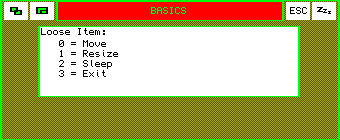
\includegraphics[width=0.75\textwidth,keepaspectratio=true]{Content/images/peas_ex0.png}
\label{fig:ExampleProgramEX0InAction}
\caption{Example program EX0 in action.}
\end{figure}


The window in Figure~\ref{fig:ExampleProgramEX0InAction} shows an outline with a green border and an
 \emph{interesting} paper colour. A white information window is
        displayed listing the various loose items in the program. The information window
        is white with a green border and black ink.

Along the very top of the window we can see the program's title -{} BASICS -{}
        in a red papered information window with a green border and ink, and the four
        loose items for MOVE and SIZE on the left with ESC and SLEEP on the right.

The window has been created by SETW\program{SETW} and the definitions are all held in the
        file EX0w\_asm which is supplied in the
 peass download from George's web site.

What follows is a slightly amended version of the program supplied by
        George. I have updated some of the comments to make then more readable and
        understandable (by me!) and in a couple of places, I have rearranged the order of
        some of the instructions -{} with George's blessings of course.

\begin{lstlisting}[firstnumber=1,caption={Ex0 - Standard Job Header}]
;----------------------------------------------------------------------
; Standard job header.
;----------------------------------------------------------------------
         bra.s     start
         dc.l      0
         dc.w      $4afb

fname    dc.w      fname_e-fname-2
         dc.b      "EX0 v1.05"
fname_e  ds.b      0
         ds.w      0

;----------------------------------------------------------------------
; Include the various Easy PEasy include files. These give us names for
; all the various offsets, vectors, traps etc used by the PE.
;----------------------------------------------------------------------
         in        win1_ass_pe_keys_pe
         in        win1_ass_pe_qdos_pt
         in        win1_ass_pe_keys_wwork
         in        win1_ass_pe_keys_wstatus
         in        win1_ass_pe_keys_wman
         in        win1_ass_pe_keys_wdef


;----------------------------------------------------------------------
; Define a few explicit equates for this example program. These are 
; offsets into the program's dataspace (relative to A6) where we store
; various bits of useful information, channel ids and so on.
;----------------------------------------------------------------------
id       equ       0
wmvec    equ       4
slimit   equ       8               ; Size - origin
\end{lstlisting}

The above is the usual QDOSMSQ job header, and so on. The various
 IN lines pull in the include files from Easy PEasy\program{EasyPEasy}.

\begin{lstlisting}[firstnumber=last,caption={Ex0 - Initialisation}]
;----------------------------------------------------------------------
; Here is when the example code really starts.
;----------------------------------------------------------------------
start    lea       (a6,a4.l),a6    ; Dataspace in A6
         bsr.s     ope             ; Open a con channel
         move.l    a0,id(a6)       ; Keep the ID safe
         moveq     #iop_pinf,d0    ; Find Pointer Environment & WMAN
         moveq     #-1,d3          ; Timeout
         trap      #3              ; Do it
         tst.l     d0              ; Did it work?
         bne       sui             ; Failed, or PE absent, bale out
         move.l    a1,wmvec(a6)    ; Keep WMAN vector safe too
         beq       sui             ; WMAN not present, bale out
         movea.l   a1,a2           ; Copy WMAN vector to A2
         lea       slimit(a6),a1   ; Buffer for results
         moveq     #iop_flim,d0    ; Find maximum size of window
         trap      #3              ; Do it
         subi.l    #$C0008,(a1)    ; Less 12, 8 from width, height
         lea       wd0,a3          ; Address of main window definition
         move.l    #ww0_0,d1       ; Size of working definition
         bsr       getsp           ; Return ALCHP'd address in A0
         movea.l   a0,a4           ; Copy to A4.
\end{lstlisting}

The section of code above carries out various initialisations and checks for
        the Pointer Environment and WMAN\program{WMAN} before allocating enough space for the working
        definition for the main window which SETW\program{SETW} stores for us
        in ww0\_0.

\begin{lstlisting}[firstnumber=last,caption={Ex0 - Loose Item Initialisation}]
;----------------------------------------------------------------------
; We need to set the status area to zeros
; and the loose items to "available" (zero).
;----------------------------------------------------------------------
         lea       wst0,a1         ; Status area address
         movea.l   a1,a0           ; Copy to A0
         moveq     #wst0_e-wst0-1,d1 ; Bytes to clear - 1

st1      clr.b     (a0)+           ; Set status to zero/available
         dbra      d1,st1          ; And repeat

         movea.l   id(a6),a0       ; Get the channel ID again
         move.l    wd_xmin+wd_rbase(a3),d1 ; Minimum size (x,y) in D1
         andi.l    #$0FFF0FFF,d1   ; Lop off the scaling factors
;                                  ; Wm_setup gets upset if you leave
;                                  ; scaling stuff attached. The x,y 
;                                  ; sizes in D1 must be actual sizes.
         jsr       wm_setup(a2)    ; Set up the working definition
\end{lstlisting}

Just before we (finally) set up the window, we need to be sure that all the
        loose items are set to available -{} in this case -{} and that the status area is
        filled with zeros. As ever, SETW\program{SETW} has put the status
        area details in an easy to find location -{} wst0 -{} and we use this to initialise
        the status area easily. Regardless of the actual size of the status area itself,
        the above code will always work.

Please note, in the above George picks the smallest window definition as the
        one to use when the program first starts. The size of the smallest definition is
        obtained from wd\_xmin + wd\_rbase(a3) and placed in D1.L with the high word
        containing the width and the low word holding the height. Because this definition
        has scaling details embedded in the top nibble of each word, these must be masked
        out before calling \pe{wm\_setup}.

The same applies if you set D1.L to zero -{} which means \emph{use the
        default (largest) definition} -{} unless the scaling factors are masked
        off, the call to \pe{wm\_setup} will return, but your window will not display correctly,
        if at all. This problem also affects the \pe{wm\_fsize} routine which returns the size,
        in D1.L, for a given definition. You \emph{must} mask off the
        scaling nibbles.

\begin{lstlisting}[firstnumber=last,caption={Ex0 - Position and Draw Window}]
         moveq     #-1,d1          ; Set the window position ...
         jsr       wm_prpos(a2)    ; ... to where the pointer is
         jsr       wm_wdraw(a2)    ; Draw the contents
\end{lstlisting}

The snippet of code above sets the window position to be where the pointer
        is on screen right now, then draws the window.

\begin{lstlisting}[firstnumber=last,caption={Ex0 - Reading the Pointer}]
wrpt     jsr       wm_rptr(a2)     ; Read the pointer
\end{lstlisting}

The above starts the pointer reading loop. This code will not return unless
        an action routine sets D0 with an error code, or, sets D4 with an event
        number.

\begin{lstlisting}[firstnumber=last,caption={Ex0 - Test for Errors or Events}]
         beq.s     no_err          ; As D0 is zero, D4 must be non zero
         bra       sui             ; Error, D0 is non zero, bale out
\end{lstlisting}

If we have returned from the read pointer loop, then D0 is holding an error
        code, or D4 holds an event number. Because the Status Register must hold the flags
        according to the value in D0 on exit from an action routine, checking for the Z
        flag being set implies that D0 is indeed holding an error.

If no error is detected, the code skips off to a label no\_err below, where
        D4 is checked for events to process, otherwise, the program dies horribly with a
        call to the sui routine supplied by George.

\begin{lstlisting}[firstnumber=last,caption={Ex0 - Console Channel Details \& Code}]
;----------------------------------------------------------------------
; Default console channel definition.
;----------------------------------------------------------------------
con      dc.w      3
         dc.b      'con'

;----------------------------------------------------------------------
; Routine to open a channel for this job.
;----------------------------------------------------------------------
ope      lea       con,a0          ; To open "con"
         moveq     #-1,d1          ; For this job
         moveq     #0,d3
         moveq     #io_open,d0
         trap      #2
         rts
\end{lstlisting}

The code above defines a console channel for our program and opens
        it.

\begin{lstlisting}[firstnumber=last,caption={Ex0 - Checking Events}]
no_err   movea.l   (a4),a1         ; Status area
         btst      #pt__can,wsp_weve(a1) ;Was it a CANCEL event?
         bne       sui             ; Yes, exit

         btst      #pt__move,wsp_weve(a1) ; Was it a MOVE event?
         beq.s     no_er1          ; No, skip
         bsr       move            ; Yes, process a MOVE
         bra.s     wrpt            ; Read pointer again

no_er1   btst      #pt__wsiz,wsp_weve(a1) ; Was it a SIZE event?
         beq       no_er2          ; No, skip
         bsr.s     resze           ; Yes, process a SIZE
         bra.s     wrpt            ; Read pointer again

no_er2   btst      #pt__zzzz,wsp_weve(a1) ; Was it a SLEEP event?
         beq.s     wrpt            ; No, read the pointer again
         move.l    #ww0_1,d1       ; Get main window button size
         move.l    #ww0_0,d2       ; Get main window size
         bsr       sleep           ; Process a SLEEP
         bra.s     wrpt            ; Read pointer again
\end{lstlisting}

The code above is executed on return from the read pointer loop with an
        event number in D4. It begins by checking to see if the CANCEL event occurred (or
        was set in an action routine) and if so, exits the program via the sui
        routine.

Assuming that the event was not CANCEL, the next check is for a MOVE event.
        If it was a MOVE, the move is handled by George's move routine and we return to
        the read pointer loop again.

The next check is for a SIZE event and if detected, we process the MOVE
        request and return to the pointer reading loop, otherwise we skip to the final
        check.

The last check we make is for a SLEEP event. If this is not a SLEEP request,
        we skip back and begin reading the pointer again. It this is a SLEEP request, we
        set the registers as required by the sleep routine by loading D1 with the current
        window size and D2 with the button window size -{} both helpfully defined by
 SETW -{} and jump into the sleep routine.

The sleep routine returns control to our code again and we skip back to
        reading the pointer. We must do this or we will never be able to know when the
        sleeping program has been wakened etc.

All of the above checks were made by looking at the individual bits in the
        window byte of the event vector.

\begin{lstlisting}[firstnumber=last,caption={Ex0 - Move Loose Item Action Routine}]
;----------------------------------------------------------------------
; Loose item action routines.
;----------------------------------------------------------------------
; MOVE
;----------------------------------------------------------------------
afun0_0  bsr       move            ; Process a MOVE

af1      move.w    wwl_item(a3),d1 ; Loose item number
         move.b    #wsi_mkav,ws_litem(a1,d1.w) ; Ask for redraw
         moveq     #-1,d3          ; Selective redraw
         jsr       wm_ldraw(a2)    ; Redraw loose items
         clr.b     ws_litem(a1,d1.w) ; Available status
         moveq     #0,d4           ; No events
         moveq     #0,d0           ; No errors
         rts                       ; Read the pointer again
\end{lstlisting}

The program demonstrates both methods of handling loose item action
        routines. MOVE and SIZE are handled within the read pointer loop and not by the
        above code which checks the event bits outside of the read pointer loop.

The action routine above, for a MOVE, carries out all the processing
        necessary to make the window move on screen. It simply calls the move routine
        supplied by George.

The code at label af1 is necessary as it resets the loose item's status to
        available -{} when a loose item is hit or done, its status changes to selected.
        Once this has been done and the loose item redrawn, D4 and D0 are set to tell the
        read pointer loop to continue, the action has been processed.

\begin{lstlisting}[firstnumber=last,caption={Ex0 - SIZE Loose Item Action Routine}]
;----------------------------------------------------------------------
; RESIZE
;----------------------------------------------------------------------                                    
afun0_1  move.l    a3,-(a7)        ; Save working register
         movea.l   ww_wdef(a4),a3  ; Window definition x,y size
         bsr.s     resze           ; Process a SIZE
         movea.l   (a7)+,a3        ; Restore pointer to loose item
         bra.s     af1             ; And reset status etc
\end{lstlisting}

The action routine above processes a SIZE request when the Size Loose Item
        is hit or done. It does this by calling code common to the action routine itself
        and called by the user level code (outside the pointer reading loop) when a SIZE
        event bit is set in the window event vector.

Unfortunately, there is no Easy PEasy\program{EasyPEasy} way to do a resize (at least, not at
        the moment) so we programmers have to do it all ourselves. As shown below.

\begin{lstlisting}[firstnumber=last,caption={Ex0 - SIZE Processing}]
;----------------------------------------------------------------------
*  To perform the resize we need to
*    a. Find the amount of resize (by wm_chwin)
*    b. Throw away the current working definition (by wm_unset)
*    c. Find the new size (by wm_fsize)
*    d. Get space for the new working definition (by getsp)
*    e. Set up the new working definition  (by wm_setup)
*    f. Position the new window  (by wm_prpos)
*    g. Draw the contents  (by wm_wdraw)
*
* Comments
*   On a.
*    We have to set the resize bit in the window byte of the
*    event vector in the status area before wm_chwin is called.
*    The change in size is returned in D1 and the window size
*    event number is returned in D4.
*
*   On c.
*    On entry to wm_fsize, D1 must contain the requested size.
*    This size must be chosen carefully. It must be no bigger
*    than the maximum in the window definition. It must be
*    smaller than the maximum size for the window layout. The
*    x-size must be a multiple of 4 (to allow proper stippling.
*    Finally the size must not be bigger than the current screen
*    size with allowance for shadow and border.
*    On exit D1 contains the actual size and D2.W contains the
*    number of the repeated section.
*    In this example we do not really need to use wm_fsize since
*    we know that D2.W will be zero and that the value in D1
*    will be that on entry (since we have a variable window).
*
*   On d.
*    The space needed is found from the label ww0_0 set in the
*    window definition.
*
*   On e.
*    For wm_setup we need on entry:
*     D1 = size
*     A0 = channel ID
*     A1 -> status area
*     A3 -> window definition
*     A4 -> space for working definition
*
*   On f.
*    On entry to wm_prpos we need the position in D1.
*    In order to ensure that the bottom right corner of the
*    resized window is in the same position as that of the old
*    we need to subtract the increase in size from the pointer
*    origin in the old window.
*    The new position is thus wd_org plus ww_xsize minus the
*    new size.
*
;----------------------------------------------------------------------   
resze    move.l    ww_xorg(a4),d7
         move.l    ww_wdef(a4),a5           Window def
         add.l     wd_xorg(a5),d7
         add.l     ww_xsize(a4),d7          Ptr pos for PRPOS (optr)
         bset      #pt__wsiz,wsp_weve(a1)
         jsr       wm_chwin(a2)             Sets change to D1 (mv)
         bclr      #pt__wsiz,wsp_weve(a1)
         move.w    wd_rbase+wd_xmin(a5),d5
         andi.w    #$fff,d5
         move.w    ww_xsize(a4),d4
         swap      d1
         sub.w     d1,d4
         cmp.w     d5,d4
         bgt.s     resze1                   D4 is greater
         move.w    d5,d4

resze1   move.w    wd_xsize(a5),d5
         cmp.w     d5,d4
         blt.s     resze2                   D4 is smaller
         move.w    d5,d4

resze2   moveq     #3,d3
         add.w     d4,d3
         andi.w    #$fffc,d3                Keep answer in D3.W  (mv)
         move.w    wd_rbase+wd_ymin(a5),d5
         andi.w    #$fff,d5
         move.w    ww_ysize(a4),d4
         swap      d1
         sub.w     d1,d4
         cmp.w     d5,d4
         bgt.s     resze3                   D4 is greater
         move.w    d5,d4

resze3   move.w    wd_ysize(a5),d5
         cmp.w     d5,d4
         blt.s     resze4                   D4 is smaller
         move.w    d5,d4

resze4   swap      d3
         move.w    d4,d3                    D3 = new mv x | y
         jsr       wm_unset(a2)
         bsr       rechp

;----------------------------------------------------------------------
; Now restrict size to the screen size less (12,8)
;----------------------------------------------------------------------
         move.l    slimit(a6),d1
         cmp.w     d3,d1
         ble       resze7                   D1 OK
         move.w    d3,d1

resze7   swap      d1
         swap      d3
         cmp.w     d3,d1
         ble       Resze8                   D1 OK
         move.w    d3,d1                    New size

resze8   swap      d1                       New limited size
         move.l    d1,d3
         jsr       wm_fsize(a2)
         move.l    d1,-(a7)                 Keep size pro tem
         move.l    #ww0_0,d1                Space needed
         bsr       getsp
         move.l    (a7)+,d1                 Replace size
         movea.l   a0,a4                    New wwd
         movea.l   id(a6),a0                Replace ID
         jsr       wm_setup(a2)

;----------------------------------------------------------------------
; The position for PRPOS is optr-mv with minimum of 4 | 2
;----------------------------------------------------------------------
         move.l    d7,d1
         swap      d1
         swap      d3
         sub.w     d3,d1
         cmpi.w    #4,d1
         bge.s     resze5                   D1 not less than 4
         move.w    #4,d1                    Set minimum of 4

resze5   swap      d1
         swap      d3
         sub.w     d3,d1
         cmpi.w    #2,d1
         bge.s     resze6                   D1 not less than 2
         move.w    #2,d1                    Set minimum of 2

resze6   jsr       wm_prpos(a2)
         jmp       wm_wdraw(a2)
\end{lstlisting}

The above code is George's way of processing a SIZE request from within an
        action routine or from user code that detected the SIZE bit set in the window
        event vector.

The other two action routines, for SLEEP and ESC, demonstrate how an action
        routine can simply set the appropriate bit in the window vector, set D4 to
        indicate an event and exit with D0 cleared.

In this case, the actions cause the pointer reading loop to return to the
        user's code where the events can be checked for (see above) and processed
        accordingly.

\begin{lstlisting}[firstnumber=last,caption={Ex0 - EXIT Loose Item Action Routine}]
;----------------------------------------------------------------------
; EXIT - set the CANCEL event in the windows event vector, put the 
; CANCEL event number in D4 and exit with D0 set to zero.
;----------------------------------------------------------------------
afun0_3  bset      #pt__can,wsp_weve(a1) ; Set CANCEL window event
         moveq     #pt__can,d4     ; ESC event number
         moveq     #0,d0           ; No errors
         rts                       ; Return to exit from reading the 
;                                  ; pointer and into the PROCESS EVENT 
;                                  ; section of the user's code.
\end{lstlisting}

First of all, the action routine for the ESC loose item. This is the
        simplest action routine as it only has to set the event bit, set D4 and D0 then
        exit. It doesn't have to reset the ESC loose item status from selected back to
        available because the program is about to exit and the user will never see the
        redrawn loose item. Simple.

\begin{lstlisting}[firstnumber=last,caption={Ex0 - SLEEP Loose Item Action Routine}]
;----------------------------------------------------------------------
; SLEEP - set the ZZZ event bit in the window event vector, put the ZZZ
; event number in D4, redraw the ZZZ loose item as available - else it
; is still selected when we wake from the button frame - then exit with
; D0 set to zero.
;----------------------------------------------------------------------
afun0_2  move.w    wwl_item(a3),d1 ; Item number for the ZZZ loose item
         move.b    #wsi_mkav,ws_litem(a1,d1.w) ; Redraw as available
         moveq     #-1,d3          ; Selective redraw
         jsr       wm_ldraw(a2)    ; Redraw loose items
         clr.b     ws_litem(a1,d1.w) ; Available status set
         bset      #pt__zzzz,wsp_weve(a1) ; Set ZZZ window event.
         moveq     #pt__zzzz,d4    ; ZZZ event number
         moveq     #0,d0           ; No errors
         rts                       ; Return to exit from reading the 
;                                  ; pointer and into the PROCESS EVENT 
;                                  ; section of the user's code.
\end{lstlisting}

The sleep loose item's action routine is almost as simple, but because the
        program will -{} hopefully -{} be awakened at some point, it has to reset the loose
        item status and redraw it.

The code above starts off by obtaining the correct loose item number and
        changing its status to indicate that it is available. It then calls \pe{wm\_ldraw} to
        redraw only those loose items asking for a status change \& redraw -{} as
        signalled by the value of minus one in D3. This prevents redrawing up to 32 loose
        items which don't need redrawing because nothing has changed.

Once redrawn, the loose item's status is set to available as well, the SLEEP
        bit is set in the window event vector, D4 is set to show the event number and we
        exit with D0 cleared to show that no errors occurred.

On return from the above two action routines, the read pointer loop will
        exit and processing will continue from the \lstinline{beq.s no_err} just after the wrpt
        label. (Many lines above!)

% lstinline resets the "last" listing line number. Damn!
\begin{lstlisting}[firstnumber=305,caption={Ex0 - Includes and Libraries}]
;----------------------------------------------------------------------
; Pull in window definition as created by SETW.
;----------------------------------------------------------------------
         in        win1_ass_pe_EX0w_asm

;----------------------------------------------------------------------
; Pull in the Easy PEasy stuff next - code routines and sprites.
;----------------------------------------------------------------------
         in        win1_ass_pe_peas_sym_lst
         lib       win1_ass_pe_peas_bin

         in        win1_ass_pe_csprc_sym_lst
         lib       win1_ass_pe_csprc_bin
\end{lstlisting}

The last few lines of code pull in the SETW\program{SETW} defined window from the file
        EX0w\_asm, then LIBs in the Easy PEasy\program{EasyPEasy} routines and the various sprites that your
        program might want to use.

\section{Coming Up...}

The next chapter in the ongoing saga of writing PE
        programs in assembler, will concentrate on application windows and their
        window menus.




\part{The Pointer Environment - Continued}

\chapterimage{chapter_head_2.pdf} % Chapter heading image
\chapter{The Return of WMAN}
\program{WMAN}

\section{Introduction}
\label{ch27-intro}%hyperlabel{ch27-intro}%

Before my recent delving into George's
 SETW\program{SETW}, his Easy PEasy\program{EasyPEasy}     utilities and my brief foray into pdf magazine production, I was walking
    through the various requirements of setting up a window definition using
    WMAN\program{WMAN}. This edition continues from where we left off but incorporates
    George's utilities into the examples. As George has made it easy to write
    Pointer Environment programs, I think we should make use of his hard work.
    Code reuse is all the rage!

However, before we start coding, we better take a moment to discuss
    Application Sub-{}Windows.

\section{Application Sub-{}Windows}
\label{ch27-appl-wins}%hyperlabel{ch27-appl-wins}%

There are a number of uses for application sub-{}windows, for the
    program's display or to hold a menu, correctly known as an
 \emph{application window menu}. An application window is a
    variable thing and as such, can be defined in a number of ways. Because of
    this, and because an application can have multiple application
    sub-{}windows, when defining our main window (or the variable parts of our
    main window) we don't have a pointer to an application window. Instead, we
    have a pointer to a list of pointers and each of these, in turn, points to
    an application window definition. The list is terminated by a zero
    word.

\begin{note}
George isn't fond of having an application window just for display purposes and points out that information windows are much, much simpler. He is, of course, correct!
\end{note}  

The following is the relevant extracts from a definition of a main
    window which contains information windows, loose items and a pair of
    application sub-{}windows.

\begin{lstlisting}[firstnumber=1,caption={Example Application Sub-Window List Definition}]
; Main window definition :
           ...
           dc.w  info_list-*       ; Pointer to information window list
           dc.w  loos_list-*       ; Pointer to list of loose items
           dc.w  appw_list-*       ; Pointer to list of app windows
           ...

; Application window list :
appw_list  dc.w  appw_0-*          ; Pointer to 1st sub-window defn
           dc.w  appw_1-*          ; Pointer to 2nd sub-window defn
           dc.w  0                 ; No more app sub-windows
\end{lstlisting}

The definition of an application sub-{}window is described
    below.

\begin{lstlisting}[firstnumber=last,caption={Example Application Sub-Window Definition}]
; Application sub-window definition :
appw_0     dc.w  192               ; Width in pixels (+ scaling)
           dc.w  119               ; Height in pixels (+ scaling)
           dc.w    4               ; X org relative to 0 in main window
           dc.w   18               ; Y org relative to 0 in main window
           dc.b  256               ; Bit 7 set = clear window
           dc.b    0               ; Shadow depth - must be 0!
           dc.w    1               ; Border width
           dc.w    0               ; Border colour
           dc.w    7               ; Paper colour
           dc.w    0               ; Pointer to pointer sprite, or 0
           dc.w    0               ; User defined setup routine, or 0
           dc.w    0               ; User defined drawing routine, or 0
           dc.w    ahit0-*         ; Hit routine
           dc.w    0               ; Sub-window control routine, or 0
           dc.w    0               ; Max X control sections (splits)
           dc.w    0               ; Max Y control sections (splits)
           dc.b    9               ; Selection key
           dc.b    0               ; Spare byte - must be 0
           ...
\end{lstlisting}

For our current needs, this definition allows us to have a simple
    application sub-{}window with no pan and scroll control bars and no menu.
    The user defined setup and drawing routines are most often defined as zero
    words to allow WMAN\program{WMAN} to do the hard work.

\section{Application Sub-{}Window Hit Routines}

The hit routine for an application sub-{}window is called from within
    the \pe{wm\_rptr} call either when you HIT in the window, or when you press the
    selection key for that sub-{}window. Similar to loose item action routines
    previously discussed, if the code exits with D0 set to zero, the \pe{wm\_rptr}
    call will resume again -{} in other words, control will not return to your
    own code just yet -{} unless the hit code sets any event bits in the event
    vector. This is slightly different from loose item action routines in this
    respect.

On entry to a sub-{}window hit routine various registers are set with
    specific parameters as defined in \tablename~\ref{tab:ApplicationSubWindowHitRoutineRegisters}


\begin{table}[htbp]
\centering
\begin{tabular}{l p{0.8\textwidth}}
\toprule
\textbf{Register} & \textbf{Description}  \\
\midrule
%
D1.L & High word = pointer X position. Low word = pointer Y position in \emph{absolute} screen coordinates. Ie, the pointer position within the \emph{entire screen} and \emph{not} within the program's window or the application sub-window itself.\\
D2.W & Selection keystroke letter, in its upper cased format, or 1 = Hit/SPACE or 2 = DO/ENTER. If D2 is -1, then the application sub-window was ``hit'' by an external keystroke. Zero indicates no key was pressed.\\
D4.B & An \emph{event number}. This can only be 0, pt\_\_do (16) or pt\_\_cancel (17) as all other events are handled by WMAN\program{WMAN}. If you have a loose item with ESC as the selection keystroke, then the loose item action routine will catch the ESC keystroke - the application sub-window hit routine will not see it if the ESC causes the program to exit.\\
A0.L & Channel id.\\
A1.L & Pointer to the status area.\\
A2.L & WMAN vector.\\
A3.L & Pointer to sub-window definition.\\
A4.L & Pointer to window working definition.\\
%
\bottomrule
\end{tabular}
\caption{Application Sub-Window Hit Routine - Registers}
\label{tab:ApplicationSubWindowHitRoutineRegisters}
\end{table}

 
Hit routines should exit with D1, D5 -{} D7, A0 and A4 preserved to
    the same value that they had on entry to the routine. D2, D4, A1 -{} A3, A5
    and A6 are undefined on exit (which means that they don't care what value
    they have.) The hit code must set the SR according to the value in D0 on
    exit.

D3, on return from a hit routine, should normally be returned as per
    its value on entry. It is not used by \pe{wm\_rptr} however, it is used by
    \pe{wm\_rptrt} (read pointer with return on timeout) from
 WMAN\program{WMAN} 1.5 onwards. Wm\_rptr ignores the upper
    word of D3. If your read pointer loop is using the \pe{wm\_rptrt} vector
    instead, and you have changed the value of D3 within the hit code, you
    must clear the high word on exit.

It is important to note that WMAN\program{WMAN}  \emph{doesn't} set the event bits for you, it is up to the
    hit code to do that for you. For example, if someone HITs the application
    window then the hit routine will be called with D2 = 1 which is also the
    case also when someone DOes the application window but the pt\_\_do bit in
    the window byte of the event vector will \emph{not} be
    set.

On exit, if D0 is clear and the status (Z) bit is set, control will
    return to the \pe{wm\_rptr} loop and not to your application's code. To return
    to your own code, the hit routine needs to set at least one event bit in
    the event vector.

If an error is detected within the hit code, then it should exit
    with the appropriate error code in D0 and the status register set
    accordingly.

\section{Example Application Window}
\label{ch27-example-appl-wins}%hyperlabel{ch27-example-appl-wins}%

As before, we now create a useful (!) demonstration program to show
    us the simplest use of an application sub window. The program will look
    like the following when completed and running:

\begin{figure}[h]
\center
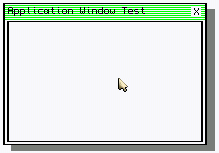
\includegraphics[width=0.5\textwidth]{Content/images/ApplTest_1.png}
\caption{Application Window Test}
\label{fig:ApplicationWindowTest}
\end{figure}

You can see from \figurename~\ref{fig:ApplicationWindowTest} how I'm sticking to accepted QDOSMSQ design     standards here can't you!

The window above consists of the following:
\begin{itemize}[itemsep=0pt]

\item{}An outline with white paper, a black single pixel border and a
        shadow. The default arrow sprite is used for the entire window.

\item{}A `caption bar' consisting of a single information window with
        green/white striped paper (paper colour 92).

\item{}Within the information window is a single information text
        object which is simply the program name.

\item{}Also located within the information window is one loose item
        containing a text object (`X') and this has the keypress code set up
        to close the window.

\item{}The remainder of the outline is filled with an application
        window, with white paper and a black single pixel border. (No shadow -{}
        they are forbidden for application windows!). This window also uses
        the default arrow sprite and has a selection key of TAB. This means
        that if you press the TAB key, the pointer will jump into the
        application sub-{}window.

\end{itemize}

The window was set up using SETW\program{SETW} as
    follows:
\begin{enumerate}
\item{When prompted for `name\$' enter
 \emph{ApplTestWin}.
}
\item{On the `Alter Text' screen.
\begin{itemize}[itemsep=0pt]

\item{}Press N for new, type `X' (without the quotes) then
            ENTER.

\item{}Press N for new, type `Application Window Test' (without the
            quotes) then ENTER

\item{}Press ESC.

\end{itemize}
}
\item{On the `Alter Sprite' screen.
\begin{itemize}[itemsep=0pt]

\item{}Press ESC.

\end{itemize}
}
\item{On the `Alter Blob' screen.
\begin{itemize}[itemsep=0pt]

\item{}Press ESC.

\end{itemize}
}
\item{On the `Alter Patt' screen.
\begin{itemize}[itemsep=0pt]

\item{}Press ESC.

\end{itemize}
}
\item{Number of main windows = 1
}
\item{Number of Loose Items = 1
}
\item{Number of Information windows = 1
}
\item{Number of IW Objects = 1
}
\item{Number of application windows = 1
}
\item{Application windows menu items = 0
}
\item{For main window 1:
\begin{itemize}[itemsep=0pt]

\item{}Shadow = 2

\item{}Border size = 1

\item{}Border colour = colour\_ql -{}>{} black

\item{}Paper colour -{} colour\_ql -{}>{} white

\item{}Sprite = arrow

\end{itemize}
}
\item{Loose Items:
\begin{itemize}[itemsep=0pt]

\item{}Press N for `system palette defaults'

\item{}Confirm N when prompted again for defaults

\item{}Border size = 1

\item{}Border colour = colour\_ql -{}>{} black

\item{}Unavailable background = colour\_ql -{}>{} white

\item{}Unavailable Ink = colour\_ql -{}>{} grey

\item{}Available background = colour\_ql -{}>{} white

\item{}Available Ink = colour\_ql -{}>{} black

\item{}Selected background = colour\_ql -{}>{} green

\item{}Selected Ink = colour\_ql -{}>{} black

\end{itemize}
}
\item{Loose Item 1:
\begin{itemize}[itemsep=0pt]

\item{}Type = text

\item{}Object -{}>{} select the `X' text object

\item{}Selection key = ESC

\end{itemize}
}
\item{Information Window 1:
\begin{itemize}[itemsep=0pt]

\item{}Border size = 0

\item{}Paper = colour\_ql -{}>{} No 92

\end{itemize}
}
\item{Object 1:
\begin{itemize}[itemsep=0pt]

\item{}Type = text

\item{}Object -{}>{} select the `Application Window Test' text
            object.

\item{}Colour = colour\_ql -{}>{} black

\item{}Xcsize = 0

\item{}Ycsize = 0

\end{itemize}
}
\item{Application Window 1:
\begin{itemize}[itemsep=0pt]

\item{}Border size = 1

\item{}Border colour = colour\_ql -{}>{} black

\item{}Paper colour = colour\_ql -{}>{} white

\item{}Sprite = arrow

\item{}Selection key = TAB

\end{itemize}
}
\item{Main window size: (Use the arrow keys to change the size, press
        ENTER when correct)
\begin{itemize}[itemsep=0pt]

\item{}Width = 200

\item{}Height = 140

\item{}Do you want a variable window = N

\item{}Set the origin to 0,0 (Press ENTER when correct)

\end{itemize}
}
\item{Loose Item 1: (Toggle hit/position with F2. Press ENTER when
        correct)
\begin{itemize}[itemsep=0pt]

\item{}Hit size = 10 x 10

\item{}Position = 186 x 3

\end{itemize}
}
\item{Information Window 1: (Toggle size/position with F2. Press ENTER
        when correct)
\begin{itemize}[itemsep=0pt]

\item{}Size = 200 x 16

\item{}Position = 0 x 0

\item{}Object position = 2 x 2

\end{itemize}
}
\item{Application Window 1: (Toggle size/position with F2. Press ENTER
        when correct)
\begin{itemize}[itemsep=0pt]

\item{}Size = 192 x 119

\item{}Position = 4 x 18

\end{itemize}
}
\end{enumerate}

When you have completed this procedure, and
 SETW\program{SETW} has exited, you should save the file
 ram1\_ApplTestWin\_asm to a safer place. The file
    should look like the following, although I have added some extra comments
    to my copy of the generated code.

\begin{lstlisting}[firstnumber=1,caption={Test Window - ApplTestWin\_asm}]
; ApplTestWin_asm

; Undefined Labels - need to be defined elsewhere in my own code.
;     ahit0   - application window 0 hit action routine.
;     afun0_0 - Loose item 0 hit action routine.

; Labels for External Use
;     wst0    - Window status area
;     wd0     - Window definition address
;     ww0_0   - Window default size
;     ww0_1   - Window button size

SYS_SPR  dc.w       0,1,2,3,4,5,6,7,8,9,10,11,12,13,14,15,16
         dc.w       17,18,19,20,21,22,23,24,25,26,27,28,29,30
         dc.w       31,32,33,34,35,36,37


; Definition of all text objects here

txt0     dc.w       txt0_e-2-txt0
         dc.b       "X"
txt0_e   ds.b       0
         ds.w       0

txt1     dc.w       txt1_e-2-txt1
         dc.b       "Application Window Test"
txt1_e   ds.b       0
         ds.w       0


; Application window list.
app_list0
         dc.w       appw0-*
         dc.w       0


; Application windows 0 definition.
appw0    dc.w       192       xsize
         dc.w       119       ysize
         dc.w       4         xorg
         dc.w       18        yorg
         dc.w       256       flag
         dc.w       1         borw
         dc.w       0         borc
         dc.w       7         papr
         dc.w       0         pspr *
         dc.w       0         setr *
         dc.w       0         draw *
         dc.w       ahit0-*   hit *
         dc.w       0         cntrl *
         dc.w       0         nxsc
         dc.w       0         nysc
         dc.b       9         skey
         dc.b       0         spr1

; Information Object(s)
pobl0    dc.w       138       xsize
         dc.w       10        ysize
         dc.w       2         xorg
         dc.w       2         yorg
         dc.b       0         type
         dc.b       0         spar
         dc.l       0         Ink, xcsize,ycsize
         dc.w       txt1-*    pobj *
         dc.w       -1

; Information window(s)
infw0    dc.w       200       xsize
         dc.w       16        ysize
         dc.w       0         xorg
         dc.w       0         yorg
         dc.w       0         flag
         dc.w       0         borw
         dc.w       526       borc
         dc.w       92        papr
         dc.w       pobl0-*   pobl *
         dc.w       -1        end

; Loose item(s)
litm0    dc.w       10,10     xsize, ysize
         dc.w       186,3     xorg, yorg
         dc.b       0,0       xjst, yjst
         dc.b       0,3       type, skey
         dc.w       txt0-*    pobj *
         dc.w       0         item
         dc.w       afun0_0-* pact *
         dc.w       -1        end

litm1    dc.w       16404,12  xsize, ysize
         dc.w       0,0       xorg, yorg
         dc.b       0,0       xjst, yjst
         dc.b       0,0       type, skey
         dc.w       0         pobj *
         dc.w       0         item
         dc.w       0         pact *
         dc.w       -1        end

; Window definition
wd0      dc.w       200       xsize
         dc.w       140       ysize
         dc.w       0         xorg
         dc.w       0         yorg
         dc.w       258       flag
         dc.w       1         borw
         dc.w       0         borc
         dc.w       7         papr
         dc.w       0         sprt *
         dc.w       1         curw
         dc.w       0         curc
         dc.w       7         uback
         dc.w       255       uink
         dc.w       0         ublob *
         dc.w       0         upatt *
         dc.w       7         aback
         dc.w       0         aink
         dc.w       0         ablob *
         dc.w       0         apatt *
         dc.w       4         sback
         dc.w       0         sink
         dc.w       0         sblob *
         dc.w       0         spatt *
         dc.w       0         help
         dc.w       200       xsize
         dc.w       140       ysize
         dc.w       infw0-*   pinfo *
         dc.w       litm0-*   plitem *
         dc.w       app_list0-*  pappl *
         dc.w       16384     xsize
         dc.w       12        ysize
         dc.w       0         pinfo *
         dc.w       litm1-*   plitem *
         dc.w       0         pappl *
         dc.w       -1

; Sizes
ww0_0    equ       290
ww0_1    equ       148

; Status Areas
wst0
         ds.b      65
wst0_e   ds.b      0
         ds.w      0
\end{lstlisting}

\section{Example Program}
\label{ch27-example-program}%hyperlabel{ch27-example-program}%

Having defined our application window test definition, we need a
    program to run it. However, we must also decide what the program is
    intended to do when running. As this is our first program with an
    application window, we will simply write some information to the
    application window when `things' happen.

I mentioned `code reuse' above, so the following is based very
    heavily on George's example code, with (I hope) all the unnecessary bits
    removed. Unnecessary, that is, for this example of mine!

The following is enough of a test harness to get our newly designed
    window up and running, but only the ESC key and the `X' loose item works.
    The rest of the program will come later.

In the source code that follows, where I use the `in' or the `lib'
    commands, you will need to replace `win1\_georgegwilt\_' with the location
    of the files being included. Unless you have exactly the same source setup
    as I do!

We start, as ever, with a standard QDOSMSQ job header and then pull
    in the various include files from Easy PEasy\program{EasyPEasy}. Three offsets into the job's
    data area are then defined.

\begin{lstlisting}[firstnumber=1,caption={ApplTest\_asm - Standard Job Header \& Equates}]
        bra.s start
        dc.l  0
        dc.w  $4afb

fname   dc.w  fname_e-fname-2
        dc.b  "Application Window Test 1"
fname_e ds.b  0
        ds.w  0

; We need the various equates files etc.

        in win1_georgegwilt_peass_keys_pe
        in win1_georgegwilt_peass_qdos_pt
        in win1_georgegwilt_peass_keys_wwork
        in win1_georgegwilt_peass_keys_wstatus
        in win1_georgegwilt_peass_keys_wman
        in win1_georgegwilt_peass_keys_wdef

id      equ 0                   ; Channel id storage
wmvec   equ 4                   ; WMAN vector storage
slimit  equ 8                   ; IOP_FLIM results - 4 words ...
;                               ; X-size, Y-size, X-org, Y-org
\end{lstlisting}

Following on from the above, we have the job's start and
    initialisation code. As the vast majority of this has been explained
    before in the introductory article on George's Easy
    PEasy\program{EasyPEasy}, I shall not go into it again here. See \emph{Easy
    PEasy Part 1} in \emph{Volume 14 Issue 3} for full
    details.

\begin{lstlisting}[firstnumber=last,caption={ApplTest\_asm - Initialisation}]
start   lea (a6,a4.l),a6        ; Make A6 point to the job's dataspace
        bsr op_con              ; Open a con channel
        move.l a0,id(a6)        ; And store the channel id
        moveq #iop_pinf,d0      ; Trap to get Pointer Information
        moveq #-1,d3            ; Timeout
        trap #3                 ; Do it
        tst.l d0                ; Is ptr_gen present?
        bne sui                 ; No, bale out via SUI
        move.l a1,wmvec(a6)     ; Yes, store the WMAN vector
        beq sui                 ; Oops! WMAN wasn't actually found

flim    movea.l a1,a2           ; The WMAN vector is required in A2
;                               ; The channel id is already in A0
        lea slimit(a6),a1       ; Result buffer
        moveq #iop_flim,d0      ; Query maximum size of window
        moveq #0,d2             ; D2 must be zero
;                               ; D3 is preserved timeout from above
        trap #3                 ; Do it (No errors)
        tst.l d0                ; Did it work?
        bne sui                 ; No, exit via SUI

        subi.l #$C0008,(a1)     ; Adjust max height & width for shadow
;                               ; and borders. 
        lea wd0,a3              ; Get address of window definition
        move.l #ww0_0,d1        ; Get size of the working definition
        bsr getsp               ; ALCHP memory and set A0 to address
        movea.l a0,a4           ; Which we save in A4
\end{lstlisting}

So far so good. Next we use a generic piece of code to go through
    the status area and set all the lose item status bytes to
    `available'.

\begin{lstlisting}[firstnumber=last,caption={ApplTest\_asm - Loose Item Initialisation}]
        lea wst0,a1             ; Status area starts here
        movea.l a1,a0           ; Copy to A0
        moveq #wst0_e-wst0-1,d1 ; How many bytes to clear - 1

st_clr  clr.b (a0)+             ; Clear one byte
        dbf d1,st_clr           ; Then the remainder
\end{lstlisting}

At this point we are just about ready to go. So, the next piece of
    code will call out the various WMAN\program{WMAN} routines to
    setup the window definition, position it on screen where the pointer
    currently is located and draw it before vanishing into the twilight zone
    that is the read pointer loop within WMAN\program{WMAN}. All
    of these have been described before so I don't go into detail.

\begin{lstlisting}[firstnumber=last,caption={ApplTest\_asm - Window Creation \& Display}]
        movea.l id(a6),a0       ; Get the channel id where we need it
;                                 A1 is the status area address
;                                 A3 is the window definition address
;                                 A4 is the working definition address
        move.l wd_xmin+wd_rbase(a3),d1 ; Get the minimum dimensions
        andi.l #$FFF0FFF,d1     ; Mask off any scaling factors
        jsr wm_setup(a2)        ; Set up the working definition

        moveq #-1,d1            ; Draw the window where the pointer is
        jsr wm_prpos(a2)        ; Position it as a primary window
        jsr wm_wdraw(a2)        ; Draw the contents
wrpt    jsr wm_rptr(a2)         ; Enter the "read pointer" loop in WMAN
\end{lstlisting}

At this point, WMAN\program{WMAN} takes over and we
    never get beyond the above code unless an event is detected -{} or set in an
    action routine -{} or an action routine flags an error. You will learn more
    about this as we add some meat to this programs workings later on.

The following code will exit from the program if an error occurred.
    The Z flag is already set or unset according to the value in D0.

\begin{note}
Of course, the following checks only work if the application sub-window hit routine, or the various loose item action routines set D4 first, then D0. Otherwise, we need to make sure that the Z flag is set according to D0 before we test it.
\end{note}

\begin{lstlisting}[firstnumber=last,caption={ApplTest\_asm - Error Handling},label={lst:ApplTestErrorHandling}]
        beq.s no_err            ; Since D0 is zero D4 is non zero
        bra sui                 ; An error occurred exit via SUI
\end{lstlisting}

If we are here, we need to check for any events that may have been
    detected or set in an action routine. In this example, we don't check
    every event, only the CANCEL event caused by the ESC key being
    pressed.

On return from the \pe{wm\_rptr} call, A0 is the channel id and A4 is the
    working definition address.

\begin{lstlisting}[firstnumber=last,caption={ApplTest\_asm - Event Handling}]
no_err  movea.l (a4),a1         ; Status area address
        btst #pt__can,wsp_weve(a1) ; Check for CANCEL event
        bne sui                 ; Exit

        bra.s wrpt              ; No more events, read pointer again
\end{lstlisting}

As mentioned above, this example currently is only checking for the
    ESC key being pressed. However, we have a loose item that can also be
    clicked to escape from the program. Rather than handling the ESC key and
    the loose item separately, we simply set the CANCEL event within the loose
    item action routine and let WMAN\program{WMAN} take care of
    it by passing control out of the read pointer loop into the above event
    handling code.

The following is the loose item action routine to do this.

\begin{lstlisting}[firstnumber=last,caption={ApplTest\_asm - ESC Loose Item Action Routine}]
; Loose item action routine

afun0_0 bset  #pt__can,wsp_weve(a1) ; Set the CANCEL event bit
        moveq #pt__can,d4         ; CANCEL event number
        moveq #0,d0               ; No errors
        rts                       ; Exit here and exit from wm_rptr too
\end{lstlisting}

Because we have an application window defined, then the following is
    the default application window hit routine. When you hit the application
    window, or press the TAB key, the following code is executed. The default
    simply sets the registers to show no errors, no events and returns control
    back to the \pe{wm\_rptr} loop.

\begin{lstlisting}[firstnumber=last,caption={ApplTest\_asm - Application Window HIT Routine}]
; Application sub-window hit routine

ahit0   moveq #0,d4
        moveq #0,d0
        rts
\end{lstlisting}

\begin{note}
The loose item action routine and application window hit routine
      names, \texttt{afun0\_0} and \texttt{ahit0} are hard coded by
 SETW\program{SETW} and, unless we physically edit the code
      generated by SETW\program{SETW}, we must use the names
 SETW\program{SETW} chooses for us.

There is a pattern to the names though, \texttt{ahit0} is the application
      sub-{}window hit routine for application sub-{}window zero. \texttt{Ahit1} would be
      the hit routine for sub-{}window 1 and so on. For loose items, you have a
      layout number and a loose item number to contend with. So \texttt{afun0\_0} is for
      layout zero and loose item zero within that layout. \texttt{Afun0\_1} is the next
      loose item within that layout, and so on.

Note also, if, as above, the hit routine sets D4 first, then D0 prior to exiting, the code that checks for errors need not execute an instruction to set the Z flag according to D0, it can simply test the Z flag immediately. See line 68 in \lstlistingname~\ref{lst:ApplTestErrorHandling} above.
\end{note}

The remainder of the code, so far, consists of helper routines and
    is shown below without any further discussion.

\begin{lstlisting}[firstnumber=last,caption={ApplTest\_asm - Console Handling}]
; Various helper routines go here...

con     dc.w con_e-con-2          ; Size of channel definition
        dc.b 'con'
con_e   equ *

op_con  lea  con,a0               ; We want a console
        moveq #-1,d1              ; For this job
        moveq #0,d3               ; Open type = "OPEN"
        moveq #io_open,d0
        trap #2                   ; Do it
        rts
\end{lstlisting}

And finally, we need to load in the window definition we generated
    using SETW\program{SETW} and all the Easy
    PEasy\program{EasyPEasy} code libraries supplied by George.

\begin{lstlisting}[firstnumber=last,caption={ApplTest\_asm - Incorporating the EasyPEasy Library}]
; Pull in our window definition file.

        in  win1_source_ApplTestWin_asm

; We need George's Easy PEasy code next.

        in  win1_georgegwilt_peass_peas_sym_lst
        lib win1_georgegwilt_peass_peas_bin

; And finally, George's sprites.

        in  win1_georgegwilt_peass_csprc_sym_lst
        lib win1_georgegwilt_peass_csprc_bin
\end{lstlisting}

Save the code as ApplTest\_asm. At least, that's
    what I called mine!

The code above can be assembled and executed and the window we
    designed a couple of issues ago will be displayed on screen. Currently it
    does nothing useful but if you press the TAB key when the pointer is
    outside the application window (but inside the main window) then you will
    see it jump into the application window. HITting the `X' loose item will
    cause the program to exit as will pressing the ESC key.

\section{Coming Up...}
\label{ch27-the-end}%hyperlabel{ch27-the-end}%

In the coming chapter we will add some code to this example to allow us to
    monitor events.



\chapterimage{chapter_head_1.pdf} % Chapter heading image
\chapter{Application Sub-{}Windows}

\section{Introduction}
\label{ch28-intro}%hyperlabel{ch28-intro}%

Last issue I left you looking at a wonderful but practically useless program - ApplTest\_asm - which displayed itself on screen and reacted only to the user clicking on a loose
        item or pressing the ESC key to quit the program. Apart from that, the most useful
        thing it did was to move the pointer into the middle of the application sub-{}window
        when the user pressed the TAB key.

This time, we get to add a little code, and see what happens when we hit an
        application sub-{}window. Let's get coding.

\section{The Hit Routine.}
\label{ch28-appl-hit}%hyperlabel{ch28-appl-hit}%

You don't actually need to have a hit routine for all your application
        sub-{}windows, there's nothing wrong with setting up an application sub-{}window in a
        program and then not having a hit routine. This is especially true if you intend
        to display information in it rather than handle user interactions and so on. As
        you will see when running the code below, the hit routine for an application
        sub-{}window gets called very frequently, so if you don't need one, don't use
        one.

You can disable the hit routine, if you don't need or want one, by setting
        the pointer to the hit routine to zero in the window definition file created by SETW\program{SETW}. 
        
\begin{note}
George isn't fond of having an application window just for display purposes and points out that information windows are much, much simpler. He is, of course, correct!
\end{note}        
 
 Now, it's time to get down to editing our new
        program.

We need to copy the two files we created last time, and rename them. So,
        copy ApplTest\_asm to ApplHitTest\_asm,
        and ApplTestWin\_asm to ApplHitTestWin\_asm. These are going to be used in our first
        experiment.

First of all, we need to change one text object in the file
 ApplHitTestWin\_asm, so edit that file and change the caption
        text to `Application Window Hit Test' from `Application Window Test 1'. Save the
        file.

Next up, we need to edit ApplHitTest\_asm. 

\begin{note}
Where possible, line numbers reference those in the file we created in the previous chapter. Lines starting at 1, will be new ones that should be inserted. Anything else will be noted in the text.
\end{note}

\begin{lstlisting}[firstnumber=5,caption={ApplTest\_asm - New Job Name}]
fname   dc.w  fname_e-fname-2
        dc.b  "Application Window Hit Test"
fname_e ds.b  0
\end{lstlisting}

Next we need to change the application sub-{}window hit routine. Look through
        the code for the routine named ahit0, which should be around line 83, and change it to the following.

\begin{lstlisting}[firstnumber=83,caption={ApplTest\_asm - New Application Window HIT Routine}]
; Application sub-window hit routine

ahit0   movem.l d1/d3/d5-d7/a0/a4,-(a7) ; Save the workers
        moveq #0,d1               ; D1.W = Application window number
        moveq #0,d2               ; D2.W = Ink colour = black
;                                   A4 already = Working definition
        jsr wm_swapp(a2)          ; Set channel id to the sub window

        movem.l a1-a2,-(a7)       ; A1 & A2 get corrupted
        lea hit,a1                ; Text string to print
        move.w ut_mtext,a2        ; Print string vector
        jsr (a2)                  ; Print the message

        lea hitter,a1             ; Hit counter location
        move.w (a1),d1            ; Hit counter value
        addq.w #1,(a1)            ; Increment counter
        move.w ut_mint,a2         ; Print integer vector
        jsr (a2)                  ; Print it

        movem.l (a7)+,a1-a2       ; Restore working registers

        movem.l (a7)+,d1/d3/d5-d7/a0/a4 ; Restore the workers

        moveq #0,d4               ; No events
        moveq #0,d0               ; No errors
        rts

; Strings and things go here

hitter  dc.w 0                    ; How many times have I been hit?

hit     dc.w hit_e-hit-2          ; Hit message
        dc.b 'HIT: '
hit_e   equ *
\end{lstlisting}

Then, right at the end, line 100, where we include our window definition, change the
        file name to suit our new name -{} from ApplTestWin\_asm to
 ApplHitTestWin\_asm.

\begin{lstlisting}[firstnumber=100,caption={ApplTest\_asm - Including the Window Definition}]
; Pull in our window definition file.

        in  win1_source_ApplHitTestWin_asm
\end{lstlisting}

Save the file. We are done.

Note in the above code, the call to \pe{WM\_SWAPP}. This sets the channel id in A0
        to point to the application sub-{}window that we specify in D1. The ink colour is
        set according to the value in D2.W and the \emph{sub-{}window is
        cleared}. If we don't do this call, we might still print to the
        application window however, if we do, it's just luck! You should
 \emph{always} ensure that the channel id in A0 has been explicitly
        pointed to the appropriate application window before attempting to print, cls, set
        paper or ink, etc when executing code within a hit routine. If you don't, any text
        printed by the code in the hit routine may well end up writing all over a loose
        item, or an information window or some random place in the window.

Obviously if you are running a program that has an application sub-{}window
        that doesn't have a hit routine, you will still need to call \pe{WM\_SWAPP} to make sure
        that the channel id in A0 points to where the sub-{}window is on screen -{} assuming
        of course, that you wish to write text to that sub-{}window as part of the
        application.

When you assemble it and execute it, note how the counter changes as you
        move the pointer over and around the application sub-{}window. It seems that you
        don't have to use the left mouse button or space bar to get a HIT. In fact using
        the right mouse button or ENTER both add 1 to the counter. The documentation says
        that \emph{If there is no keystroke, or the keystroke is not the selection
        keystroke for a loose menu item or an application sub-{}window, then, if the pointer
        is within a sub-{}window, the hit routine is called, or else the loose menu item
        list is searched to find a new current item}.

Press ESC to stop the program, then execute it again, try to keep the
        pointer outside the application sub-{}window. Now, press TAB. The pointer jumps into
        the sub-{}window, but what happens to the counter? It increases by two rather than
        one on every \emph{subsequent} press of the TAB key.

This happens when you press some other key combinations, F1 increases the
        counter by two as well. Other letter or digit keys increment the counter by
        one.

I wonder why? Maybe, in the case of F1, the keystroke itself causes a hit
        and then the HELP event that the keystroke causes forces another hit? This doesn't
        explain the TAB key having the same effect though -{} that doesn't cause a hit. I
        mentioned above that a hit routine gets called very frequently didn't I?

\begin{note}
Ok, as an aside, I tested it. Using QMON2, I
            put a breakpoint at Ahit0 -{} the entry point for the application sub-{}window hit
            routine. On hitting the TAB key, I got a breakpoint. Looking at the registers
            I found that the pointer position in D1 was well outside my window limits,
            very strange. D2, the keystroke was set to -{}1 to indicate that an
 \emph{external keystroke} fired the hit routine. There was no
            event in D4 -{} it was zero and D6, an undefined register was zero. So far so
            good, I noted down the registers and let the program continue.

It immediately stopped at the hit routine again, this time the pointer
            position had moved into my screen bounds from wherever it had been in
            hyperspace. D2 was now zero to indicate that no key has been pressed. D4 was
            still zero -{} so no events either. D6 had changed to \$80. Wonder what that
            means?

Letting the program run again, I pressed F1 this time -{} without moving
            the pointer. Once again I hit the breakpoint. I could see the pointer position
            in D1 had not changed, D4 still showed no events, D2 showed no key press and
            D6 had returned to zero.

And again, I let the program run and it broke again. D6 was back at \$80
            again. D1, D2, D4 were all unchanged (as were all the other registers.)

I hit space this time, when I let QMON\program{QMON} run
            the program. As expected this showed a \$01 in D2 -{} the key press for a HIT is
            converted to \$01, D6 was showing zero again. D4 still showed no events.

Once more, QMON\program{QMON} let the program run and this
            time, I pressed ENTER. D4 showed the value \$10 or the event number for a DO.
            The key press in D2 was set to \$02 for a DO. D6 was zero and nothing else
            changed.

Finally, I pressed ESC to quit. Now, according to the docs, I should
            have stopped at Ahit0 again with D4 showing the CANCEL event, however, as
            documented above there was a loose item which had the ESC key set as the
            selection keystroke. That code was executed to exit from the program, rather
            than the application sub-{}window hit code being called with D4 set to the
            CANCEL event number.
\end{note}

\section{The Advanced Hit Routine.}
\label{ch28-appl-adv-hit}%hyperlabel{ch28-appl-adv-hit}%

So, that's our first very simple hit test program done and dusted. It's
        quite simple but quite useless, all it does is show you the running total of hits
        in the window. You will soon get bored of it.

For our next trick, we shall improve the utility to display full details of
        what data gets passed to the hit routine. Copy
 ApplHitTest\_asm to ApplHitTest\_2\_asm,
        and ApplHitTestWin\_asm to
 ApplHitTestWin\_2\_asm.

As before, we need to change one text object in the file
 ApplHitTestWin\_2\_asm, so edit that file and change the
        caption text to `Application Window Hit Test 2' from `Application Window Hit Test'.
        Save the file.

Next up, we need to edit ApplHitTest\_2\_asm.

\begin{lstlisting}[firstnumber=1,]
fname   dc.w  fname_e-fname-2
        dc.b  "Application Window Hit Test 2"
fname_e ds.b  0
\end{lstlisting}

Next we need to change the application sub-{}window hit routine. Look through
        the code for the routine named ahit0 and change it to the following.

\begin{lstlisting}[firstnumber=1,]
; Application sub-window hit routine

ahit0   movem.l d1/d3/d5-d7/a0/a4,-(a7) ; Save Hit Routine registers

        bsr.s apinit              ; Initialise the sub-window
        bsr.s ptrpos              ; Show the pointer position
        bsr.s keystr              ; Display keystroke
        bsr events                ; Print event details

        movem.l (a7)+,d1/d3/d5-d7/a0/a4 ; Restore Hit Routine registers
        moveq #0,d0               ; No errors
        rts
\end{lstlisting}

The main code in this advanced hit routine is simple -{} it stacks all the
        registers that we require to preserve throughout the hit routine, and makes calls
        to a few helper routines to carry out one specific task. I admit, this is not the
        most efficient method, but it allows me to split the code into manageable chunks
        for describing in the text.

\begin{lstlisting}[firstnumber=1,]
; Helper - Initialise the sub-window.

apinit  movem.l d1-d2/a1-a2,-(a7) ; We need these registers later
        moveq #0,d1               ; D1.W = Application window number
        moveq #0,d2               ; D2.W = Ink colour
;                                   A4 = Working definition
        jsr wm_swapp(a2)          ; Set channel id to the sub window
        movem.l (a7)+,d1-d2/a1-a2 ; Ptr position & keystroke back again
        rts
\end{lstlisting}

The first subroutine called simply initialises the application sub-{}window
        setting the ink to black and forcing the channel Id to cover the application
        sub-{}window. Any registers corrupted by the routine are stacked on entry and
        restored on exit.

\begin{lstlisting}[firstnumber=1,]
; Helper - Display pointer position details.

ptrpos  movem.l d1-d3/a1,-(a7)    ; These get corrupted here
        lea ptrx,a1               ; 'Ptr_x: '
        bsr.s print               ; Print it

        move.l (a7),d1            ; Restore the old D1 again.

        swap d1                   ; Lo = pointer X, Hi = pointer Y 
        bsr pr_int2               ; Print pointer X

        lea ptry,a1               ; ' Ptr_Y: '
        bsr.s print               ; Print it

        movem.l (a7)+,d1-d3/a1    ; Retrieve other registers
        bsr.s pr_int2             ; Print pointer Y
        rts
\end{lstlisting}

The code above preservers all registers that will be corrupted and then
        displays the current pointer position in absolute screen coordinates. These are
        relative to the 0,0 position of the entire screen and not relative to the 0,0
        position of the actual main window for our application. 

\begin{lstlisting}[firstnumber=1,]
; Helper - Display keystroke

keystr  movem.l d1-d3/a1,-(a7)    ; These get corrupted here
        lea keystk,a1             ; 'Key: '
        bsr.s print               ; Print it

        move.l 4(a7),d2           ; Retrieve D2
        cmpi.b #-1,d2             ; External keystroke?
        bne.s k_hit               ; no, try a HIT

        lea keyext,a1             ; 'External'
        bra.s k_doit              ; Print & exit

k_hit   cmpi.b #1,d2              ; HIT?
        bne.s k_do                ; No, try a DO

        lea keyhit,a1             ; 'HIT'
        bra.s k_doit              ; Print & exit

k_do    cmpi.b #2,d2              ; DO?
        bne.s k_zero              ; No, must be a key code or zero

        lea keydo,a1              ; 'DO'
        bra.s k_doit              ; Print & exit

k_zero  cmpi.b #0,d2              ; Zero = no key pressed
        bne.s k_keys              ; Has to be a key press

        lea keyzero,a1            ; 'No key'
        bra.s k_doit              ; Print & exit

k_keys  move.w d2,d1              ; Need keystroke in D1.B
        moveq #io_sbyte,d0
        moveq #-1,d3
        trap #3                   ; Print keystroke
        bra.s k_done              ; Exit

k_doit  bsr.s print               ; Print message
k_done  movem.l (a7)+,d1-d3/a1    ; Restore working registers
        rts
\end{lstlisting}

The code above starts, as usual, by preserving the working registers. It
        then checks the value in D2 to see which, if any Key was pressed to cause a hit in
        the application sub-{}window. D2 can be any of the following:
\begin{itemize}

\item{}Negative 1 = the activation key was pressed to place the pointer
                into the application sub-{}window.


\item{}1 -{} HIT -{} the left mouse button was clicked within the application
                sub-{}window, or the space bar was pressed.


\item{}2 -{} DO -{} the right mouse button or the ENTER key was pressed while
                the pointer was within the application sub-{}window.


\item{}Zero -{} no key or mouse button has been pressed.


\item{}Anything else -{} this will be the upper cased key code for the actual
                key that was pressed.

\end{itemize}

If the TAB key is pressed, you might briefly see the `external keystroke'
        message flash across the screen quickly followed by `No key pressed' -{} as I
        mentioned previously, pressing TAB (the activation key for the sub-{}window) results
        in two separate calls to the hit routine.

\begin{lstlisting}[firstnumber=1,]
; Helper - Print event details

events  movem.l d1-d3/a1,-(a7)    ; Save the usual bunch
        lea event,a1              ; 'Event: '
        bsr.s print               ; Print message
        move.w d4,d1              ; Event number
        bsr.s pr_int2             ; Print it
        movem.l (a7)+,d1-d3/a1    ; Restore the workers
        rts
\end{lstlisting}

Finally, we have the helper routine that displays details of whatever event
        was detected which caused the hit routine to be activated. As ever, the code
        starts by preserving the working registers and then examines D4 to see which, if
        any, event took place.

\begin{lstlisting}[firstnumber=1,]
; Helper - Print string at (a1) to channel in A0. 
; Then CLS to end of line.

print   move.w ut_mtext,a2        ; Vector to print string
        jsr (a2)                  ; Print it
        movem.l d1/d3/a1,-(a7)    ; These get corrupted
        moveq #sd_clrrt,d0        ; CLS to end of cursor line
        moveq #-1,d3
        trap #3                   ; Do it
        movem.l (a7)+,d1/d3/a1    ; Restore
        rts


; Helper - Print word int at (a1) to channel in A0.

pr_int  move.w (a1),d1            ; Get word to print
pr_int2 move.w ut_mint,a2         ; Print word int vector
        jsr (a2)                  ; Print it
        rts
\end{lstlisting}

The above routines are called by the main sub-{}routines themselves to display
        messages and numeric values on screen. The various messages are defined in the
        code below.

\begin{lstlisting}[firstnumber=1,]
; Assorted TEXT messages etc follow.

ptrx    dc.w ptrx_e-ptrx-2
        dc.b 'Ptr_X: '
ptrx_e  equ *

ptry    dc.w ptry_e-ptry-2
        dc.b ' Ptr_Y: '
ptry_e  equ *

keystk  dc.w keystk_e-keystk-2
        dc.b $0a
        dc.b 'Key: '
keystk_e equ *

keyhit  dc.w keyhit_e-keyhit-2
        dc.b '1 = HIT'
keyhit_e equ *

keydo   dc.w keydo_e-keydo-2
        dc.b '2 = DO'
keydo_e equ *

keyext  dc.w keyext_e-keyext-2
        dc.b '-1 = External Keystroke'
keyext_e equ *

keyzero dc.w keyzero_e-keyzero-2
        dc.b '0 = No Key Pressed'
keyzero_e equ *

event   dc.w event_e-event-2
        dc.b $0a
        dc.b 'Event: '
event_e equ *
\end{lstlisting}

So, there you have it, a small and incredibly inefficient hit routine to
        display some of the data that are passed into an application sub-{}window hit
        routine when it is executed. I have not bothered to display the various window
        definition addresses etc -{} if you wish, feel free to create a 32 bit long to
        hexadecimal conversion routine to display these values.

I have deliberately left these out in an effort to save space in the
        magazine\footnote{\emph{QL Today}} -{} my listings can get a tad on the long side!

There is one final change we need to make to our source code, right at the
        end, where we include our window definition, change the file name to
 ApplHitTestWin\_2\_asm.

\begin{lstlisting}[firstnumber=1,]
; Pull in our window definition file.

        in  win1_source_ApplHitTestWin_2_asm
\end{lstlisting}

Save the file. We are done.

When assembled and executed, the code in the hit routine displays a few
        details of register settings on entry to the hit routine. It's not very useful,
        but shows the pointer position in absolute screen coordinates as opposed to
        relative to the start of the actual sub-{}window (which would have been a lot more
        useful in my opinion), it shows the key press if any key was pressed and it shows
        which event, if any, occurred. Remember, only a limited number of events get
        through to a application sub-{}window hit routine.

If you press the TAB key and watch closely, you might see a brief message
        saying `External Keystroke' before the text is replaced by `No key pressed'. This
        shows, once again, that the TAB key results in two calls to the hit
        routine.

\section{Conclusion}

One thing has become obvious from even these two little routines, an
        application sub-{}window results in a huge number of hits! Even moving the pointer
        within a sub-{}window results in multiple hits. It might be better to display
        information -{} whatever the application needs to print on screen -{} to an
        information window instead. This should certainly save on processing time.
        However, as I mentioned above, only use a hit routine if you absolutely need
        one.

Failing this, the ideal hit routine for an application window should be
        hugely efficient -{} and it should exit quickly when it doesn't need to do any
        [further] processing, rather than just doing everything each time the code is
        entered.

\section{Coming Up...}
\label{ch28-the-end}%hyperlabel{ch28-the-end}%

The next chapter continues looking at application sub-{}windows, but we will be
        loading them with menus!



\chapterimage{chapter_head_2.pdf} % Chapter heading image
\chapter{Application Sub-{}Window Menus}

\section{Introduction}
\label{ch29-intro}%hyperlabel{ch29-intro}%

At the end of the last chapter, I promised to continue looking at
    Application Sub-{}Windows by adding Application Sub-{}Window Menus to them.

Effectively, there are two different types of application sub-{}window
    menus:
\begin{itemize}[itemsep=0pt]

\item{}Static -{} which are defined in the program source code and never
        change;

\item{}Dynamic -{} which may change as the applications runs.

\end{itemize}

In this chapter, we shall look at the Static Application Sub-{}Window
    Menus only. In a future chapter, we shall look at Dynamic Menus as they are much more difficult to set up correctly.

\section{Static Application Sub-{}Window Menus}
\label{ch29-app-menu-static}%hyperlabel{ch29-app-menu-static}%

Static menus, as I shall call them from this point onwards, are
    created by the developer as s/he writes the program. As the program runs,
    static menus do not change -{} other than setting entries to available or
    unavailable as required.

We can use SETW\program{SETW} to create static menus.
    All that is required is for the developer to decide on the menu options,
    the required layout of rows and columns, and what to do when the user
    clicks on an option -{} although this latter option is not needed by
 SETW\program{SETW}, only in the application's code.

We need to design a new window using SETW\program{SETW}, so proceed to execute the
    utility and proceed as follows:
\begin{enumerate}
\item{When prompted for `name\$' enter
 \emph{AppMenuTest1}. I'd like to use the name \emph{AppMenuTest1Win},
          but that is too big for SETW. When
          finished, the file \emph{AppMenuTest1\_asm} is easily
          renamed to \emph{AppMenuTest1Win\_asm}.
}
\item{On the `Alter Text' screen.
\begin{itemize}[itemsep=0pt]

\item{}Press N for new, type `X' (without the quotes) then
            ENTER.


\item{}Press N for new, type `Application Menu Test 1' (without the
            quotes) then ENTER


\item{}Press N for new, type `One' then enter.
\item{}Press N for new, type `Two' then enter.
\item{}Press N for new, type `Three' then enter.
\item{}Press N for new, type `Four' then enter.
\item{}Press N for new, type `Five' then enter.
\item{}Press N for new, type `Six' then enter.
\item{}Press N for new, type `Seven' then enter.
\item{}Press N for new, type `Eight' then enter.
\item{}Press N for new, type `Nine' then enter.
\item{}Press N for new, type `Ten' then enter.

\item{}Press ESC.


\end{itemize}
}
\item{On the `Alter Sprite' screen.
\begin{itemize}[itemsep=0pt]

\item{}Press ESC.

\end{itemize}
}
\item{On the `Alter Blob' screen.
\begin{itemize}[itemsep=0pt]

\item{}Press ESC.

\end{itemize}
}
\item{On the `Alter Patt' screen.
\begin{itemize}[itemsep=0pt]

\item{}Press ESC.

\end{itemize}
}
\item{Number of main windows = 1.
}
\item{Number of Loose Items = 1.
}
\item{Number of Information windows = 2.
}
\item{For Information Window 1 of 2, the number of IW Objects =
        1.
}
\item{For information windows 2 of 2, the number of IW Objects =
        0.
}
\item{Number of application windows = 1.
}
\item{Application windows menu items = 10.
}
\item{For main window 1:
\begin{itemize}[itemsep=0pt]

\item{}Shadow = 2


\item{}Border size = 1


\item{}Border colour = colour\_ql -{}>{} black


\item{}Paper colour -{} colour\_ql -{}>{} white


\item{}Sprite = arrow

\end{itemize}
}
\item{Presentation of loose Items:
\begin{itemize}[itemsep=0pt]

\item{}Press N for `system palette defaults'


\item{}Confirm N when prompted again for defaults


\item{}Border size = 1


\item{}Border colour = colour\_ql -{}>{} black


\item{}Unavailable background = colour\_ql -{}>{} white


\item{}Unavailable Ink = colour\_ql -{}>{} grey


\item{}Available background = colour\_ql -{}>{} white


\item{}Available Ink = colour\_ql -{}>{} black


\item{}Selected background = colour\_ql -{}>{} green


\item{}Selected Ink = colour\_ql -{}>{} black

\end{itemize}
}
\item{Loose Item 1:
\begin{itemize}[itemsep=0pt]

\item{}Type = text


\item{}Object -{}>{} select the `X' text object


\item{}Selection key = ESC

\end{itemize}
}
\item{Information Window 1:
\begin{itemize}[itemsep=0pt]

\item{}Border size = 0


\item{}Paper = colour\_ql -{}>{} No 92

\end{itemize}
}
\item{Object 1:
\begin{itemize}[itemsep=0pt]

\item{}Type = text


\item{}Object -{}>{} select the `Application Window Test' text
            object.


\item{}Colour = colour\_ql -{}>{} black


\item{}Xcsize = 0


\item{}Ycsize = 0

\end{itemize}
}
\item{Information Window 2:
\begin{itemize}[itemsep=0pt]

\item{}Border size = 1


\item{}Border colour = ql\_colour -{}>{} black


\item{}Paper = colour\_ql -{}>{} white

\end{itemize}
}
\item{Application Window 1:
\begin{itemize}[itemsep=0pt]

\item{}Border size = 1


\item{}Border colour = colour\_ql -{}>{} black


\item{}Paper colour = colour\_ql -{}>{} white


\item{}Sprite = arrow


\item{}Selection key = TAB


\item{}Presentation of Menu Items\begin{itemize}[itemsep=0pt]

\item{}Select N for system palette defaults


\item{}Select N for defaults, again.


\item{}Border size = 1.


\item{}Border colour = ql\_colour -{}>{} black.


\item{}Unavailable background = ql\_colour -{}>{} white.


\item{}Unavailable ink = ql\_colour -{}>{} grey.


\item{}Available background = ql\_colour -{}>{} white.


\item{}Available ink = ql\_colour -{}>{} black.


\item{}Selected background = ql\_colour -{}>{} green.


\item{}Selected ink = ql\_colour -{}>{} black.


\item{}Scroll arrow = ql\_colour -{}>{} white.


\item{}Scroll bar = ql\_colour -{}>{} black.


\item{}Scroll background = ql\_colour -{}>{} red.


\item{}When prompted for the ten menu items, select the text
                  items `One' through `Ten'. Give each one a selection key of
                  the digit that matches the number described by the text
                  object. For example, `One' has a key of `1', `Two' has `2'
                  and so on up to `Ten' which has selection key `0'
                  (Zero).

\end{itemize}


\end{itemize}
}
\item{Main window size: (Use the arrow keys to change the size, press
        ENTER when correct)
\begin{itemize}[itemsep=0pt]

\item{}Width = 220


\item{}Height = 140


\item{}Do you want a variable window = N


\item{}Set the origin to 0,0 (Press ENTER when correct)

\end{itemize}
}
\item{Loose Item 1: (Toggle hit/position with F2. Press ENTER when
        correct)
\begin{itemize}[itemsep=0pt]

\item{}Hit size = 10 x 10


\item{}Position = 206 x 3

\end{itemize}
}
\item{Information Window 1: (Toggle size/position with F2. Press ENTER
        when correct)
\begin{itemize}[itemsep=0pt]

\item{}Size = 220 x 16


\item{}Position = 0 x 0


\item{}Object position = 2 x 2

\end{itemize}
}
\item{Information Window 2: (Toggle size/position with F2. Press ENTER
        when correct)
\begin{itemize}[itemsep=0pt]

\item{}Size = 216 x 14


\item{}Position = 2 x 125

\end{itemize}
}
\item{Application Window 1: (Toggle size/position with F2. Press ENTER
        when correct)
\begin{itemize}[itemsep=0pt]

\item{}Size = 208 x 104


\item{}Position = 2 x 18

\end{itemize}
}
\end{enumerate}

When you have completed this procedure, and
 SETW\program{SETW} has exited, you should save the file
 ram1\_AppMenuTest1\_asm to a safer place and rename it
    to AppMenuTest1Win\_asm. The file should look similar
    to the following, although I have added some extra comments to my copy of
    the generated code.

\section{The Generated Code}
\label{ch29-app-menu-code}%hyperlabel{ch29-app-menu-code}%

The file should look similar to the following, although I have added
    some extra comments to my copy of the generated code.

\begin{note}
I have removed a few sections of the following file in order to
      reduce duplication of chunks of code in the magazine. These sections are
      discussed below.
\end{note}

\begin{lstlisting}[firstnumber=1,caption={AppMenuTest1Win\_asm}]
; AppMenuTest1Win_asm.

; Undefined Labels - need to be defined elsewhere in my own code.

;        ahit2_0 - menu item 0, hit routine.
;        ahit2_1 - menu item 1, hit routine.
;        ahit2_2 - menu item 2, hit routine.
;        ahit2_3 - menu item 3, hit routine.
;        ahit2_4 - menu item 4, hit routine.
;        ahit2_5 - menu item 5, hit routine.
;        ahit2_6 - menu item 6, hit routine.
;        ahit2_7 - menu item 7, hit routine.
;        ahit2_8 - menu item 8, hit routine.
;        ahit2_9 - menu item 9, hit routine.
;        asmnu0  - User defined setup routine.
;        adraw0  - User defined draw routine.
;        ahit0   - application window 0 hit action routine.
;        afun0_0 - Loose item 0 hit action routine.

; Labels for External Use
;     mst0    - menu items status area
;     wst0    - Window status area
;     wd0     - Window definition address
;     ww0_0   - Window default size
;     ww0_1   - Window button size

SYS_SPR  dc.w     0,1,2,3,4,5,6,7,8,9,10,11,12,13,14,15,16,17,18,
                  19,20,21,22,23,24,25,26,7,28,29,30,31,32,33,
                  34,35,36,37

; Text object for "Close" loose item.
txt0     dc.w      txt0_e-2-txt0
         dc.b      "X"
txt0_e   ds.b      0
         ds.w      0

; Text object for caption bar.
txt1     dc.w      txt1_e-2-txt1
         dc.b      "Application Menu Test 1"
txt1_e   ds.b      0
         ds.w      0

;----------------------------------------------------------------------
; **** Text objects for the menu items. Removed - see text.

; **** Menu items list. Removed - see text.

; **** Row list. Removed - see text.

; **** Spacing list. Removed - see text.
;----------------------------------------------------------------------

; Application window list.
app_list0
         dc.w      appw0-*
         dc.w      0


;----------------------------------------------------------------------
; **** Application window 0 definition. Removed - see text.
;----------------------------------------------------------------------


; Information Object(s).
pobl0
         dc.w      138       xsize
         dc.w      10        ysize
         dc.w      2         xorg
         dc.w      2         yorg
         dc.b      0         type
         dc.b      0         spar
         dc.l      0         spce
         dc.w      txt1-*    pobj *
         dc.w      -1

; Information Window(s).
infw0
         dc.w      220       xsize
         dc.w      16        ysize
         dc.w      0         xorg
         dc.w      0         yorg
         dc.w      0         flag
         dc.w      0         borw
         dc.w      526       borc
         dc.w      92        papr
         dc.w      pobl0-*   pobl *
         dc.w      216       xsize
         dc.w      14        ysize
         dc.w      2         xorg
         dc.w      125       yorg
         dc.w      0         flag
         dc.w      1         borw
         dc.w      0         borc
         dc.w      7         papr
         dc.w      0         pobl *
         dc.w      -1        end

; Loose Item(s).
litm0
         dc.w      10,10     xsize, ysize
         dc.w      206,3     xorg, yorg
         dc.b      0,0       xjst, yjst
         dc.b      0,3       type, skey
         dc.w      txt0-*    pobj *
         dc.w      0         item
         dc.w      afun0_0-* pact *
         dc.w      -1        end

litm1
         dc.w      16404,12  xsize, ysize
         dc.w      0,0       xorg, yorg
         dc.b      0,0       xjst, yjst
         dc.b      0,0       type, skey
         dc.w      0         pobj *
         dc.w      0         item
         dc.w      0         pact *
         dc.w      -1        end

; Window definition
wd0
         dc.w      220       xsize
         dc.w      140       ysize
         dc.w      0         xorg
         dc.w      0         yorg
         dc.w      258       flag
         dc.w      1         borw
         dc.w      0         borc
         dc.w      7         papr
         dc.w      0         sprt *
         dc.w      1         curw
         dc.w      0         curc
         dc.w      7         uback
         dc.w      255       uink
         dc.w      0         ublob *
         dc.w      0         upatt *
         dc.w      7         aback
         dc.w      0         aink
         dc.w      0         ablob *
         dc.w      0         apatt *
         dc.w      4         sback
         dc.w      0         sink
         dc.w      0         sblob *
         dc.w      0         spatt *
         dc.w      0         help
         dc.w      220       xsize
         dc.w      140       ysize
         dc.w      infw0-*   pinfo *
         dc.w      litm0-*   plitem *
         dc.w      app_list0-*         pappl *
         dc.w      16384     xsize
         dc.w      12        ysize
         dc.w      0         pinfo *
         dc.w      litm1-*   plitem *
         dc.w      0         pappl *
         dc.w      -1

; Sizes
ww0_0    equ       670
ww0_1    equ       148

; Status Areas:
; Menu item status area.
mst0     ds.b      10
mst0_e   ds.b      0
         ds.w      0

; Window status area.
wst0     ds.b      65
wst0_e   ds.b      0
         ds.w      0
\end{lstlisting}

Much of the above is similar to when was discussed in a previous
    article. If you think back to that article on application sub-{}windows, we
    simply used the hit routine to print text all over the application
    sub-{}window. That was about as simple as it gets -{} other than not actually
    having a hit routine I suppose! Adding a menu to an application
    sub-{}window means we have quite a lot more work to do at the coding stage
    as we have to consider the following:
\begin{itemize}[itemsep=0pt]

\item{}Defining the menu objects -{} these can be text, sprite etc. Every
        menu item must be defined.


\item{}Defining the menu items list -{} when we have defined each menu
        object, we then have to build a list of all the menu items that we
        wish to include in our final menu.


\item{}Defining the menu row list -{} when we have the menu items list
        defined, we amalgamate that list into a menu row list which defines
        the start and end of each row in the menu.


\item{}Defining the spacing lists -{} the row list defines the hit size
        and the spacing for each row and each column in the menu.


\item{}Define the application sub-{}window -{} menus need their own section
        in the application sub-{}window definition.

\end{itemize}

So much to do just to show a menu in a window, lets get on and do
    it.

\section{Menu Objects}
\label{ch29-app-menu-objects}%hyperlabel{ch29-app-menu-objects}%

The first stage is to define the various objects that will be
    incorporated into the menu. In this example, I have used ten separate text
    objects (as they are the simplest). You can use any of the various Pointer
    Environment object types if you wish. The code generated by
 SETW\program{SETW} for these items is as follows.

\begin{lstlisting}[firstnumber=1,caption={AppMenuTest1Win\_asm - Menu Objects}]
; **** Text objects for the menu items.

txt2     dc.w      txt2_e-2-txt2
         dc.b      "One"
txt2_e   ds.b      0
         ds.w      0


; **** Txt3 through txt10 deleted for brevity.


txt11    dc.w      txt11_e-2-txt11
         dc.b      "Ten"
txt11_e  ds.b      0
         ds.w      0
\end{lstlisting}

As you can see from the above, I have omitted to show text objects
    txt3 through txt10 as there is really no need to take up space in the
    magazine with repetitive data.

The above code simply defines ten separate text objects -{} `One',
    `Two', ..... `Nine' and `Ten' to be used, later, in our static
    menu.

You should be aware, also, that the line numbers above (and indeed, in the following snippets) bear no resemblance to the ones in the original file.

\section{Menu Items (and Index) List}
\label{ch29-app-menu-item-list}%hyperlabel{ch29-app-menu-item-list}%

The next section of code that I have removed from the main listing
    above is the menu items list. This is shown below, but please note that
    once again, I have removed the vast majority of the code for
    brevity.

\begin{lstlisting}[firstnumber=last,caption={AppMenuTest1Win\_asm - Menu Item List}]
; **** Menu items list. 

meos2    dc.b      1,0             ; x_justification, y_justification 
         dc.b      0,49            ; Item type, selection key
         dc.w      txt2-*          ; Pointer to object
         dc.w      0               ; Item number. (-1 for indexes)
         dc.w      ahit2_0-*       ; Hit routine for this item
;                                  ; Zero for indexes


; NOTE: Menu items 1 through 8 removed here for brevity.


         dc.b      1,0             ; x_justification, y_justification 
         dc.b      0,48            ; Item type, selection key
         dc.w      txt11-*         ; Pointer to object
         dc.w      9               ; Item number. (-1 for indexes)
         dc.w      ahit2_9-*       ; Hit routine for this item
;                                  ; Zero for indexes
\end{lstlisting}

The label meos2 is the start of the menu items list. We told SETW\program{SETW}
    that there would be 10 items, and so, there will be 10 menu items in this
    list. Each one has the structure described in \tablename~\ref{tab:ApplicationSubWindowMenuItemListEntry}.

\begin{table}[htbp]
\centering
\begin{tabular}{c c p{0.7\textwidth}}
\toprule
\textbf{Offset} & \textbf{Size} &\textbf{Description}  \\
\midrule
%
0 & 1 & X (Horizontal) justification.
\begin{itemize}[itemsep=0pt]
\item{} -ve = Right justified
\item{}0 = Centred
\item{}+ve = Left Justified
\end{itemize}
The justification value is the number of pixels from the edge of the hit area that the object is
to be positioned at.\\

1 & 1 & Y (Vertical) justification.
\begin{itemize}[itemsep=0pt]
\item{}-ve = Bottom justified
\item{}0 = Centred
\item{}+ve = Top Justified
\end{itemize}
The justification value is the number of pixels from the edge of the hit area that the object is
to be positioned at.\\

2 & 1 & Item type:
\begin{itemize}[itemsep=0pt]
\item{}0 - Text object
\item{}2 - Sprite object
\item{}4 - Blob object
\item{}6 - Pattern object
\end{itemize}
\\

3 & 1 & Selection key, upper cased if necessary.\\

4 & 2 & Relative pointer to the actual object.\\

6 & 2 & Item number. If this is an index items list, set to -1 for all items.\\

8 & 2 & relative pointer to the hit/action routine for this particular item. For index item lists, must be zero.\\
%
\bottomrule
\end{tabular}
\caption{Application Sub-Window Menu Item List Entry}
\label{tab:ApplicationSubWindowMenuItemListEntry}
\end{table}

 


Each item in a menu items list is 10 bytes in length.

Looking at the first menu object generated by
 SETW\program{SETW}, we see that it is left justified and one
    pixel from the start of the left end of the hit area. Vertically, it is
    centred within the hit area. It is a text object and has a selection key
    of 49, which is the code for a digit `1' on the keyboard. The text object
    itself is the text `One' as shown above in the preceding section. The item
    is numbered zero and the hit routine for this item is defined to be at
    label ahit2\_0.

So far, so good. We have defined a list of objects and then gathered
    them into a list of menu items. The menu items list -{} in this case -{} is in
    a contiguous section of memory, it need not be so. The row list defines
    the menu ordering, that comes next.

The above structure is used to define menu item lists and also index
    lists. An index is drawn by the \pe{WM\_INDEX} vector (which also draws pan and
    scroll bars \& arrows -{} if necessary). Indices are best thought of as
    the row and column headings -{} similar to a spreadsheet, for example, where
    columns have letters and rows have numbers to identify them.

WMAN\program{WMAN} takes
    care of aligning the indices with the contents of the static menu.

\section{Row List}
\label{ch29-app-menu-row-list}%hyperlabel{ch29-app-menu-row-list}%

The row list takes the various menu items, defined above, and
    organises them into rows -{} surprisingly enough. For every row you wish to
    have in your menu, you need a single row list entry. As SETW\program{SETW} tries to make
    as few rows and/or columns as it can -{} it tries to fit as much as possible
    into a given space -{} what SETW\program{SETW} generates may not be what you want. In the
    default case for our SETW\program{SETW} session, we have been given two rows and thus,
    five columns, for our ten menu items.

Our generated row list is as follows:

\begin{lstlisting}[firstnumber=last,caption={AppMenuTest1Win\_asm - Row List}]
; **** Row list.

drow0    dc.w      0+meos2-*       ; Pointer to row 0 start = item 0.
         dc.w      50+meos2-*      ; Pointer to row 0 end = item 4.

         dc.w      50+meos2-*      ; Pointer to row 1 start = item 5.
         dc.w      100+meos2-*     ; Pointer to row 1 end = item 9.
\end{lstlisting}

Each row list item contains two pointers, the first is to the start
    of the first entry in the menu items list entry for this row. The second
    pointer is to the first byte past the end of the last menu items list
    entry for this row.

Given the above then, we can see that the first row, starting at
    label drow0, begins at meos2 (relative to the pointer itself -{} as usual).
    Meos2 is a list of 10 sets of 10 byte entries defining all ten items in
    our menu. The first row ends at meos2 + 50, which happens to be the very
    first byte of the menu items list for menu item number 5 (ie, the sixth
    menu item -{} we count from zero)

The second row list entry starts at meos2 + 50 and ends at meos2 +
    100. These pointers are to menu items list item number 5 and at the first
    byte past the very last menu items list entry. As the following diagram
    attempts to display:

\begin{lstlisting}[frame=none,numbers=none,caption={Relationship between the Row List \& Menu Items List} ]
Meos2+0     Menu Item 0 <-----+          Start of row 0.   
Meos2+10    Menu Item 1       |  
Meos2+20    Menu Item 2       |
Meos2+30    Menu Item 3       |
Meos2+40    Menu Item 4       |
Meos2+50    Menu Item 5 <--------+--+    End of row 0, start of row 1.
Meos2+60    Menu Item 6       |  |  |  
Meos2+70    Menu Item 7       |  |  |  
Meos2+80    Menu Item 8       |  |  |
Meos2+90    Menu Item 9       |  |  |
Meos2+100   equ  *      <--------------+ End of row 1.
                              |  |  |  | 
Drwo0       Pointer to -------+  |  |  |
            Pointer to ----------+  |  |
            Pointer to -------------+  |
            Pointer to ----------------+
\end{lstlisting}

If the menu items list is a single chunk of memory, then each row
    start pointer is equal to the previous row end pointer -{} except for the
    first row. As in the example above, the end pointer for row 0 is the same
    address as the start pointer for row 1.

Now that we have our rows defined, we have to set up the spacing
    lists for each row and each column in the menu.

\section{Spacing Lists}
\label{ch29-app-menu-space-lists}%hyperlabel{ch29-app-menu-space-lists}%

Each menu item in our static menu has a given hit area and a
    spacing. The hit area defines where the pointer can be to make the item
    beneath it the current item, this is normally indicated by a border being
    drawn around the current item. A HIT or a DO within the hit area, or a
    press of the selection keystroke while the pointer is within the
    application sub-{}window, will cause the appropriate menu item action
    routine to be executed.

The spacing defines how many pixels across -{} or down depending on
    whether this is the column or row spacing list -{} there are between the
    start of `this' menu item and the start if the `next' one. The spacing
 \emph{must} include an allowance for the border to be drawn
    around the current item.

\begin{lstlisting}[firstnumber=42,caption={AppMenuTest1Win\_asm - Spacing Lists}]
; **** Spacing lists.

; Spacing list. Defines width of hit area for each COLUMN and spacing
; between columns. (5 columns.)

spls0    dc.w      34      ; Hit area width column 0
         dc.w      36      ; Space between this column and the next.

         dc.w      34      ; Hit area width column 1
         dc.w      36      ; Space between this column and the next

         dc.w      34      ; Hit area width column 2
         dc.w      36      ; Space between this column and the next

         dc.w      34      ; Hit area width column 3
         dc.w      36      ; Space between this column and the next

         dc.w      34      ; Hit area width column 4
         dc.w      36      ; Space between this column and the next


; Spacing list. Defines height of hit area for each ROW and spacing
; between rows. (2 rows.)

spls1    dc.w      10      ; Hit area height row 0
         dc.w      12      ; Space between this row and the next

         dc.w      10      ; Hit area height row 1
         dc.w      12      ; Space between this row and the next
\end{lstlisting}

The first list above, at label spls0 defines the columns in our
    menu. We already know that SETW\program{SETW} has decreed
    that there shall be five columns and two rows, so the column spacing list
    has five entries, one for each column. Each entry consists of a pair of
    words -{} the first defines the width of the column (or the height of the
    row) and the second defines the space between this column and the
    next.

In the example above, we see that SETW\program{SETW} has calculated that our
    widest text object is 5 characters wide -{} this corresponds to `Three',
    `Seven' and `Eight' -{} and has allocated 34 pixels of hit area for each
    column. The spacing for each columns is set to the (border width * 2) plus
    the hit area width. It must be twice the border width as there is a border
    on each side (or top \& bottom).

The spacing list for the rows shows a height of ten pixels for the
    hit area and taking the border into consideration again, a spacing of 12
    pixels between the tops of each row.

\section{Menu Section of Application Window Definition}
\label{ch29-app-menu-win-def}%hyperlabel{ch29-app-menu-win-def}%

The application window definition needs an extra section adding
    after the normal definition, to cover the need for a static menu. In
    addition, two entries in the normal definition part are amended (from what
    we used for an application sub-{}window without a menu -{} see last time) to
    point to the:
\begin{itemize}[itemsep=0pt]

\item{}User defined setup routine, or zero if not required.


\item{}User defined drawing routine, or zero if not required.

\end{itemize}

The new style application window definition is as follows:

\begin{lstlisting}[firstnumber=1,caption={AppMenuTest1Win\_asm - Application Window Definition}]
; **** Application window 0 definition.

appw0    dc.w      208      ; Width in pixels (+ scaling)
         dc.w      104      ; Height in pixels (+ scaling)
         dc.w      2        ; X origin, relative to 0 in main window
         dc.w      18       ; Y origin, relative to 0 in main window
         dc.w      256      ; Flag - bit 7 set = clear window
;                           ;      - bit 1 set = disable cursor keys
         dc.w      1        ; Border width
         dc.w      0        ; Border colour
         dc.w      7        ; Paper colour
         dc.w      0        ; Pointer to pointer sprite, or 0 for arrow
\end{lstlisting}

The first part is exactly as we used last time, nothing different to
    see here. Following the above, we have this:

\begin{lstlisting}[firstnumber=last,caption={AppMenuTest1Win\_asm - Application Window Definition}]
; Note the following for menus.

         dc.w      asmnu0-* ; User defined setup routine, or 0
         dc.w      adraw0-* ; User defined drawing routine, or 0
         dc.w      ahit0-*  ; Application window hit routine
         dc.w      0        ; Control routine, or 0
         dc.w      0        ; Max X control sections (splits)
         dc.w      0        ; Max Y control sections (splits)
         dc.b      9        ; Selection key
         dc.b      0        ; Spare byte - must be 0
\end{lstlisting}

The first two entries in the above definition are the new ones.
    These are our pointers to a user defined setup routine and a user defined
    drawing routine. You will notice that the application window still has
    its own hit routine, even though it contains a menu and each and every
    menu item has a dedicated hit routine of its own. Note also, in this small
    example,that our settings for the pan and scroll sections are all unused.
    We'll come back to those in a future chapter.

The user defined setup code would normally consist of a single line
    as follows:

\begin{lstlisting}[firstnumber=1,caption={AppMenuTest1Win\_asm - Application Window Setup Routine}]
asmnu0  jmp wm_smenu(a2)    ; Vector $08
\end{lstlisting}

Similarly, the user defined drawing routine need only perform the
    following tasks:

\begin{lstlisting}[firstnumber=last,caption={AppMenuTest1Win\_asm - Application Window Drawing Routine}]
adraw0  jmp wm_index(a2)    ; Vector $34
        bne.s adexit        ; Bale out on errors
        jmp wm_mdraw(a2)    ; Vector $20
adexit  rts        
\end{lstlisting}

The call to \pe{WM\_INDEX} is not required unless your menu has been
    defined to have sections and/or index items\footnote{George Gwilt has discovered that anything to do with these index items is not actually implemented in the WMAN code. Looks like Tony Tebby had a good idea, that couldn't be fulfilled.}. What are index items? Think
    of a spreadsheet, each row has a number and each column has a letter.
    These are the index items. Our example is not using index items, however,
    if it did then we would set them up exactly as per the menu items list,
    except, for indexes the list entries have no hit routine (set to zero) and
    the item number is always -{}1.

\begin{note}
If the pointer to the user defined drawing routine is zero, then
 WMAN\program{WMAN} will still draw the application
      sub-{}window's border and, unless the flag is set to say `do not clear',
      will clear it to the defined paper colour. If you find missing menus in
      your application sub-{}windows, check that you have a drawing
      routine!
\end{note}

Following on from the above, there is a brand new section dedicated
    to the menu.

\begin{lstlisting}[firstnumber=23,caption={AppMenuTest1Win\_asm - Application Window Menu Area Definition}]
; The following section is required when an application sub-window
; contains a menu.

         dc.w      mst0-wst0 ; Pointer to menu status area. (See text)

         dc.w      1        ; Current Item, border width
         dc.w      0        ; Current Item, border colour

         dc.w      7        ; Unavailable background colour
         dc.w      255      ; Unavailable ink colour
         dc.w      0        ; Unavailable blob pointer
         dc.w      0        ; Unavailable pattern pointer

         dc.w      7        ; Available background colour
         dc.w      0        ; Available ink colour
         dc.w      0        ; Available blob pointer
         dc.w      0        ; Available pattern pointer

         dc.w      4        ; Selected background colour
         dc.w      0        ; Selected ink colour
         dc.w      0        ; Selected blob pointer
         dc.w      0        ; Selected pattern pointer

         dc.w      5        ; Number of columns in the menu
         dc.w      2        ; Number of rows in the menu
         dc.w      0        ; X offset to start of menu
         dc.w      0        ; Y offset to start of menu
         dc.w      spls0-*  ; Pointer to column spacing list
         dc.w      spls1-*  ; Pointer to row spacing list
         dc.w      0        ; Pointer to column index list
         dc.w      0        ; Pointer to row index list
         dc.w      drow0-*  ; Pointer to menu row list
\end{lstlisting}

The first new entry we need is a pointer to the menu items status
    area. This has been defined for us, by SETW\program{SETW}, at
    label mst0. There should be a single byte for each menu item. Note
    however, that we need to have this status area pointer defined as relative
    to the window status area. Hence the calculation in the above
    definition.

\begin{note}
This fact is not very clearly documented in the PE documentation.
      I had an extended conversation with George on this setting as I had
      never seen the fact that the menu status area pointer is relative to the
      window status area -{} George had a pencilled in note in his copy of the
      documentation indicating this need. Obviously, I didn't.
\end{note}

Next up, we see the menu attributes -{} border width and colour, item
    paper and ink, blobs and patterns for unavailable, available and selected
    items.

After the attributes section, we define the menu itself with details
    of how many columns there are, how many rows, offsets to the start of the
    menu and the pointers to the various sections discussed above.

\section{Application Sub-{}Window Menu Item Hit Routines}
\label{ch29-app-menu-item-hit}%hyperlabel{ch29-app-menu-item-hit}%

In addition to the application sub-{}window's own hit routine, as
    described previously, each and every item in the menu (Static or dynamic)
    may also have a hit routine. This routine could be a single one for all,
    or a separate one for each menu item. It depends on how the program is
    designed.

\begin{note}
Whenever a program has a static or dynamic menu, there
 \emph{must} be a hit routine for the application
      sub-{}window containing the menu. The absolute minimum code in the hit
      routine is as follows:

\begin{lstlisting}[firstnumber=1,caption={AppMenuTest1Win\_asm - Application Window Hit Routine}]
ahit0   jmp wm_hit(a2)            ; Vector $34
\end{lstlisting}

If you do not have the above code present in the hit routine for
      the application sub-{}window, then when you attempt to hit or do a menu
      item, nothing will work. The above code does not need an \opcode{RTS}.
\end{note}

On entry to a menu item hit routine various registers are set with
    specific parameters as described in \tablename~\ref{tab:MenuItemHitRoutineRegisters}.


\begin{table}[htbp]
\centering
\begin{tabular}{l p{0.8\textwidth}}
\toprule
\textbf{Register} &\textbf{Description}  \\
\midrule
%
D1.L & Virtual column/row for the hit menu item.\\
D2.W & Item number.\\
D4.L & An event number. This can only be 0 or pt\_\_do (16).\\
A0.L & Channel id.\\
A1.L & Pointer to the menu status area.\\
A2.L & WMAN vector.\\
A3.L & Pointer to sub-window definition.\\
A4.L & Pointer to window working definition.\\
%
\bottomrule
\end{tabular}
\caption{Menu Item Hit Routine Registers}
\label{tab:MenuItemHitRoutineRegisters}
\end{table}

Registers not mentioned above are free for use as they are not used
    by the hit routine.

Hit routines should exit with D5 -{} D7, A0 and A4 preserved to the
    same value that they had on entry to the routine. D1 -{} D3, A1 -{} A3, A5 and
    A6 are undefined on exit (which means that they don't care what value they
    have.) D4.B must be either zero or a window event to be set on
    exit.

D0 should contain zero or an error code and the SR must be set
    according to the value in D0 on exit.

\begin{note}
D3, on return from a hit routine, should normally be returned as
      per its value on entry. It is not used by \pe{WM\_RPTR} however, it is used by
      \pe{WM\_RPTRT} (read pointer with return on timeout) from
 WMAN\program{WMAN} 1.5 onwards. Wm\_rptr ignores the upper
      word of D3. If your read pointer loop is using the \pe{WM\_RPTRT} vector
      instead, and you have changed the value of D3 within the hit code, you
      must clear the high word on exit.
\end{note}

On exit, if D0 is clear and the status (Z) bit is set, control will
    return to the \pe{WM\_RPTR} loop and not to your application's code. To return
    to your own code, the hit routine needs to set at least one event bit in
    the event vector which can be done by returning a suitable value in D4.B
    on exit.

If an error is detected within the hit code, then it should exit
    with the appropriate error code in D0 and the status register set
    accordingly.

\section{Coming Up...}
\label{ch29-the-end}%hyperlabel{ch29-the-end}%

So, that's the end of this exciting chapter. We have designed a
    window and looked deep into the structures involved in defining a static
    menu. 
    
In the upcoming chapter we'll add some code and play around. We might even see if
    it's possible to take the design from SETW\program{SETW} and
    massage it to suit our own needs and considerations.



\chapterimage{chapter_head_1.pdf} % Chapter heading image
\chapter{Creating and Using Libraries With GWASL}

\section{Introduction}
\label{ch30-intro}%hyperlabel{ch30-intro}%

At the end of the last issue, I promised to continue looking at
    Application Sub-{}Windows by adding some code to our menu enabled program.
    Unfortunately, due to the current very busy situation at work, and a mild
    dose of tendonitis in my thumb, I'm having to do a lot of one-{}handed
    typing these days which is slowing me down a lot. To this end, I'm taking
    a break from application menus for a wee while, and this issue, my article
    will be small -{} but hopefully, perfectly formed -{} looking at how we can
    create and use our own libraries of useful routines with
 GWASL\program{Gwasl}.

\section{The Library Code}
\label{ch30-app-menu-code}%hyperlabel{ch30-app-menu-code}%

The following is the complete code for a small library that allows
    your own assembly code to clear various parts of the screen. I apologise
    for the briefness of this article, but as I said, I'm typing one handed at
    the moment.

The code should be typed into a file named
 lib\_cls\_asm or something similar.

\begin{lstlisting}[firstnumber=1,caption={Example Library - Lib\_cls\_asm},label={lst:LibClsAsm}]
;=========================================================;
; lib_cls_asm.                                            ;
;=========================================================;
; A small library to demonstrate the use of same in GWASL ;
; It's not particularly useful, it only demonstrates a    ;
; point!                                                  ;
;=========================================================;
; All routines expect the channel id in A0.L.             ;
; All routines assume infinite timeout.                   ;
; All regsiters are preserved, except D0.L.               ;
; Error codes are returned in D0.L and the Z flag.        ;
;=========================================================;

cls_screen equ $20
cls_top    equ $21
cls_bottom equ $22
cls_line   equ $23
cls_end    equ $24

infinity   equ -1

;---------------------------------------------------------
; CLEAR_SCREEN - Clears entire screen.                    
;---------------------------------------------------------
clear_screen  moveq #cls_screen,d0
              bra.s just_do_it

;---------------------------------------------------------
; CLEAR_TOP - Clears top of screen.                       
;---------------------------------------------------------
clear_top     moveq #cls_top,d0
              bra.s just_do_it

;---------------------------------------------------------
; CLEAR_BOTTOM - Clears bottom of screen.                 
;---------------------------------------------------------
clear_bottom  moveq #cls_bottom,d0
              bra.s just_do_it

;---------------------------------------------------------
; CLEAR_TO_EOL - Clear to end of cursor line.             
;---------------------------------------------------------
clear_to_eol  moveq #cls_end,d0
              bra.s just_do_it

;---------------------------------------------------------
; CLEAR_LINE - Clears entire cursor line.                 
;---------------------------------------------------------
clear_line    moveq #cls_line,d0

just_do_it    movem.l d1/d3/a1,-(a7)
              moveq #infinity,d3
              trap #3
              movem.l (a7)+,d1/d3/a1
              tst.l d0
              rts
\end{lstlisting}

So, you can see that there's not much to it. 

That's the end of step one. The next step is to assemble the file
    using GWASL\program{Gwasl} in the normal manner, fix any
    errors, and create an output file most likely named
 lib\_cls\_bin. In addition to the binary file, there
    will be another symbol file named lib\_cls\_sym     created. We need that file shortly, however, it isn't in a format we can
    use just yet.

Once all errors have been removed and the source assembled, we are
    ready to move onto creating our library. In actual fact, half of the
    library is already created -{} lib\_cls\_bin -{} but we
    need to convert the symbol file into a text file that we can include in
    our own source code in order to actually call the routines in the
    library.

Execute the utility named sym\_bin\program{Sym\_bin} in your
    gwasl directory. The layout of the screen should look pretty familiar if
    you have used GWASL\program{Gwasl} frequently. Choose option 1
    as normal, and type in the path to the lib\_cls\_sym file.

After a couple of seconds, you can choose the option to exit. Our
    work is done!

Sym\_bin\program{Sym\_bin} has taken the binary formatted
 lib\_cls\_sym file and created from it a new text file
    names lib\_cls\_sym\_lst. If you open this in an editor,
    it will look something like the following:

\begin{lstlisting}[firstnumber=1,caption={Example Library - Lib\_cls\_sym\_lst},label={lst:LibClsSymLst},language={}]
CLS_SCREEN    EQU   $00000020
CLS_TOP       EQU   $00000021
CLS_BOTTOM    EQU   $00000022
CLS_LINE      EQU   $00000023
CLS_END       EQU   $00000024
INFINITY      EQU   $FFFFFFFF

CLEAR_SCREEN  EQU   *+$00000000
JUST_DO_IT    EQU   *+$00000012
CLEAR_TOP     EQU   *+$00000004
CLEAR_BOTTOM  EQU   *+$00000008
CLEAR_TO_EOL  EQU   *+$0000000C
CLEAR_LINE    EQU   *+$00000010
\end{lstlisting}

You can see that all the equates defined in our source code have
    been made visible as well as offsets to the various routines. These
    offsets are the actual addresses within the
 lib\_cls\_bin file where the individual routines start.
 

It would be nice if there was some way for equates etc within a
    library to be invisible from outside it without us having to do too much
    extra work, however, as far as I'm aware, it's not possible to define an
    equate as `local' -{} similar to SuperBasic. What we can do is delete the
    top few lines leaving only the offsets to the routines. Edit the file to
    delete the lines from CLS\_SCREEN down to INFINITY. 

Next, create a new file containing these two lines, call it
 lib\_cls\_in:

\begin{lstlisting}[firstnumber=1,caption={Example Library - Lib\_cls\_in},label={lst:LibClsIn}]
              in    win1_gwasl_libs_lib_cls_sym_lst
              lib   win1_gwasl_libs_lib_cls_bin 
\end{lstlisting}

And that's all there is to it. To use the code simply include the
    following at the end of your own assembly code: 

\begin{lstlisting}[firstnumber=1,caption={Example Library - Invoking the Library},label={lst:LibClsInvoke}]
              in    win1_gwasl_libs_lib_cls_in
\end{lstlisting}

Obviously, your paths will be different from mine, so change
    accordingly to suit your own system. 

I have combined the IN and the LIB commands into one single file
    because I like to do as little typing as possible. You need not do this
    and to use the library, simply add the two lines above into the end of
    your own code at some point.

To demonstrate the code, all you need is something like this. Not
    shown in this example are other libraries that I use to set colours, open
    screens etc. 

\begin{lstlisting}[firstnumber=1,caption={Example Library - Brief Example of Use},label={lst:LibClsExampleUse}]
start         bsr   open_scr       ; Open scr_ channel return id in A0
              bsr   set_colours    ; Set paper, strip and ink preserves
;                                  ; all registers except D0.L
              bsr   clear_screen   ; Clear screen  
              ...                  ; Etc

              in  win1_gwasl_libs_lib_cls_in
              in  win1_gwasl_libs_lib_defaults_in
              in  win1_gwasl_libs_lib_colours_in
\end{lstlisting}

\section{End Of Chapter 30}
\label{ch30-the-end}%hyperlabel{ch30-the-end}%

In the next chapter I'll continue where I left off at the end of the previous chapter. I shall also be
    looking at the recent changes to EasyPEasy\program{EasyPEasy}.





%=================================================================
% LibGen is still broken, so is not included here, yet. When it's
% fixed, I'll probably do a spearate "book" - maybe even in a 
% different colour, who knows?
%=================================================================

%\part{LibGen -{} A User Friendly Library Generator}

%\chapterimage{chapter_head_2.pdf} % Chapter heading image
%\chapter{LibGen -{} Library Generator -{} Part 1}

\section{Introduction}
\label{ch31-intro}%\hyperlabel{ch31-intro}%

In the last chapter, I looked at the creation and use of libraries
    with Gwasl\program{Gwasl}. George and I had a bit of an
    email conversation we had about how to work around the problem of only
    exposing the required routines in the libraries we create without exposing
    the internal working routines. For example, in my small example library, I
    would only expose the various CLEAR\_xxx routines, but
    not the internal JUST\_DO\_IT routine. Also, it is not
    required to expose any of the equates used internally by the library -{}
    simply because they may conflict with your own equates used elsewhere in
    the program and because, by the time the library is assembled, the equates
    have been converted into absolute values anyway.

George mentioned editing the library source code, setting a new
    equate with a given prefix, to the routines you wish to expose, similar to
    the following:

\begin{lstlisting}[firstnumber=1,]
LB_CLEAR_SCREEN equ clear_screen
\end{lstlisting}

In the above, you can see that I've set
 LB\_CLEAR\_SCREEN equal to
 CLEAR\_SCREEN. When the symbol file is converted to
    text, it will have the following in it:

\begin{lstlisting}[firstnumber=1,]
...
CLEAR_SCREEN    EQU     *+$00000000
LB_CLEAR_SCREEN EQU     *+$00000000
JUST_DO_IT      EQU     *+$00000012
...
\end{lstlisting}

You can see, that CLEAR\_SCREEN and
 LB\_CLEAR\_SCREEN are the same. George proposed that a
    SuperBasic program could be quickly written to extract only those equates
    prefixed by, for example, `LB\_' and this extracted file could then be used
    to expose only the chosen routines.

I liked this idea, but I'm sort of wary about having to edit my
    source code and add extra equates whenever I write a new routine. Equally,
    this is an assembler tutorial and at present I'm writing about the Pointer
    Environment, so how about a useful -{} yes, the first one -{} utility to read
    in a sym\_lst file, display all the code offset equates (and only those)
    and when the user has selected the desired items, write out a valid file
    that can be included. This issue's article is that very utility!

\section{The SYM\_LST File Format}
\label{ch31-sym-lst-format}%\hyperlabel{ch31-sym-lst-format}%

Once symbol file has been converted to text by running George's
 SYM\_BIN utility, the format is quite
    simple.\footnote{It is indeed simple, but don't base any assumptions on the fact that all of George's symbol file listings will be in this format. Those produced by the Gwasl assembler's sym\_bin utility are slightly different from those created by the Gwass assembler's sym\_bin utility. Ask me how I know! Oh yes, the internal binary format of the two assemblers' sym files are different too. Shame.}
\begin{itemize}[itemsep=0pt]

\item{}Columns 0 to 29 hold the label.

\item{}Columns 30 to 35 hold ``EQU''.

\item{}Columns 36 onwards hold the equate value, or the code
        offset.

\end{itemize}

However, it matters not for this utility anyway, because all I'm
    doing is extracting the entire line from the file and adding it to a menu
    so that the user can select or deselect it at will. What does matter,
    however, is the difference between a code offset and a value in the file.
    Look again at the example above and note that my original equates simply
    show a hexadecimal value, while the code offsets show a similar hex value,
    prefixed by the two characters `*+' (Asterisk and plus). My utility,
 LibGen\program{LibGen}, only extracts the latter.

\section{LibGen}
\label{ch31-Lib-Gen}%\hyperlabel{ch31-Lib-Gen}%

I've chosen LibGen\program{LibGen} as my utility name.
    The finished screen will hopefully look very similar to the screen shot in Figure~\ref{fig:WhatLibGenShouldLookLike}

\begin{figure}[h]
\center
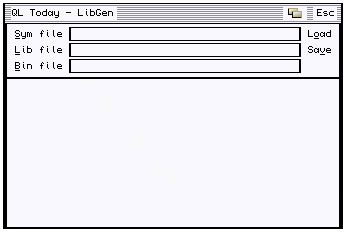
\includegraphics[width=0.65\textwidth]{Content/images/libgen_1.png}
\caption{What LibGen Should Look Like!}
\label{fig:WhatLibGenShouldLookLike}
\end{figure}


Along the top is a green/white (paper 92) caption bar which is
    simply an information window. The actual title is itself embedded in
    another small information window with white paper. The move loose item and
    the Esc loose items are embedded within the main caption bar. To keep code
    sizes to a minimum, there is no Size or Sleep loose items in this
    utility.

Moving down the screen there is a large information window with a
    black border and white paper containing the 5 loose items -{} Sym file, Lib
    file, Bin file, Load and Save, and three further information Windows, each
    with white paper and a black border.

The largest part of the window is taken up by an application window
    at the bottom. This too has white paper and a black border. This is where
    we will hold the code offset lines from the symbol file.

In operation, you click on `sym file' to allow the name of the
    sym\_lst file in question to be loaded. If the file loads, the `\_sym\_lst'
    extension is removed and replaced with `\_lib' for the `Lib file' and
    `\_bin' for the `Bin file'. You can, however, edit these auto-{}generated
    names by hitting the appropriate loose item.

When happy with the names, hit the `Load' loose item to read in the
    file. The application window will fill up with appropriate options from
    the file and you will be able to choose the ones you wish to keep. By
    default everything is selected, you only need to deselect the ones you
    don't want to keep. I'm working on the assumption that you will want to
    keep more than you don't, so it should be easier to deselect the few than
    select the many.

Once happy with your selection, hit the `Save' loose item and the
    selected entries will be copied to the `Lib file' along with a line to
    include the `Bin file', as follows:

\begin{lstlisting}[firstnumber=1,]
CLEAR_SCREEN  EQU     *+$00000000
CLEAR_TOP     EQU     *+$00000004
CLEAR_BOTTOM  EQU     *+$00000008
CLEAR_TO_EOL  EQU     *+$0000000C
CLEAR_LINE    EQU     *+$00000010

              lib     win1_gwasl_libs_lib_cls_bin
\end{lstlisting}

Now all you need to do is add one line to your program, as
    follows:

\begin{lstlisting}[firstnumber=1,]
              in    win1_gwasl_libs_lib_cls_lib
\end{lstlisting}

Hopefully, this is a lot easier than editing source code, adding
    extra equates, and running a SuperBasic program to extract them and so
    on.

\section{Window Design}
\label{ch31-lib-gen-window-design}%\hyperlabel{ch31-lib-gen-window-design}%

Make sure that you download the latest versions of
 SETW\program{SETW} and Easy PEasy\program{EasyPEasy}     from \url{http://gwiltprogs.info/page2.htm} as George has recently updated these to make our lives much easier. We
    will be using the new features of Easy PEasy\program{EasyPEasy} in
    this utility. We begin by designing our window with
 SETW\program{SETW}. Now, contrary to my own instructions
    above, I have to declare here that I'm not yet using the latest version of
 SETW\program{SETW}! I'm also abbreviating the prompts etc in
    the following steps to try and keep coding to a minimum.
\begin{enumerate}
\item{Enter a name, I used libgenwin for mine, but feel free to make
        up your own.
}
\item{Enter the following text objects by pressing the `N' key, then
        typing in the text:
\begin{itemize}[itemsep=0pt]

\item{}QL Today -{} LibGen


\item{}Esc


\item{}Sym file


\item{}Lib file


\item{}Bin file


\item{}Load


\item{}Save

\end{itemize}

Press ESC when done.
}
\item{For the sprites, blobs and patters, simple press Esc as we have
        none of those.
}
\item{There is one single main window.
}
\item{There are 7 loose items within it.
}
\item{There are 6 information windows.
}
\item{Information windows 1 to 4 have no objects, number 5 has one,
        and number 6 has none.
}
\item{There will be one application window, but it has no menu items.
        (We will build the menu dynamically.)
}
\item{The main window has the following attributes:
\begin{itemize}[itemsep=0pt]

\item{}Shadow size 2


\item{}Border size 1, border colour is QL Black.


\item{}Paper colour is QL White.


\item{}Select the default arrow sprite for the pointer.

\end{itemize}
}
\item{When prompted, twice, to select default settings for loose
        items, chose `N' both times. We will enter our own settings.
}
\item{The current item border size is 1 and the colour is QL
        Black.
}
\item{Unavailable attributes are:
\begin{itemize}[itemsep=0pt]

\item{}Background colour is QL White.


\item{}Ink colour is QL Grey.

\end{itemize}
}
\item{Available attributes are:
\begin{itemize}[itemsep=0pt]

\item{}Background colour is QL White.


\item{}Ink colour is QL Black.

\end{itemize}
}
\item{Selected attributes are:
\begin{itemize}[itemsep=0pt]

\item{}Background colour is QL Green.


\item{}Ink colour is QL Black.

\end{itemize}
}
\item{For the 7 loose items, set them up as follows:
\begin{enumerate}[itemsep=0pt]

\item{}Type is text, choose the `Esc' text, no selection
            key.


\item{}Type is text, choose the `Esc' text again, no selection key.
            We will fix this later as we need a sprite.


\item{}Type is text, choose the `Sym file' text, selection key is
            `S' and underlined.


\item{}Type is text, choose the `Lib file' text, selection key is
            `L' and underlined.


\item{}Type is text, choose the `Load' text, selection key is `O'
            and underlined.


\item{}Type is text, choose the `Save' text, selection key is `V'
            and underlined.


\item{}Type is text, choose the `Bin file' text, selection key is
            `B' and underlined.

\end{enumerate}

Loose item 2 uses the same `Esc' text as loose item 1 but we
        will fix this in the code that gets generated. I haven't yet found a
        way of getting the standard sprites into a
 SETW generated program.
}
\item{For the 6 information windows, set them up as follows:
\begin{enumerate}[itemsep=0pt]

\item{}Border size zero, paper QL 92.


\item{}Border size 1, colour QL Black, paper QL White.


\item{}Border size 1, colour QL Black, paper QL White.


\item{}Border size 1, colour QL Black, paper QL White.


\item{}Border size 0, paper QL White. When prompted for an object,
            choose Text `QL Today -{} LibGen', set the ink to QL Black and the
            two CSizes to zero.


\item{}Border size 1, colour QL Black, paper QL White.

\end{enumerate}
}
\item{The application window needs the following:
\begin{itemize}[itemsep=0pt]

\item{}Border size 1.


\item{}Colour QL Black.


\item{}Paper QL White.


\item{}Choose the standard arrow sprite.


\item{}Set the selection key to TAB.

\end{itemize}
}
\item{There now follows a session of pressing arrow keys and F2 etc to
        size and position all the loose items, information windows to build
        our window. The main window itself is first:
\begin{itemize}[itemsep=0pt]

\item{}The size is 336 by 224.


\item{}The window is not a variable one.


\item{}The pointer origin is 50 by 37.

\end{itemize}
}
\item{The 7 loose items should be sized and positioned as
        follows:
\begin{enumerate}[itemsep=0pt]

\item{}24 by 13 at 308 by 3.


\item{}24 by 13 at 278 by 3.


\item{}50 by 14 at 8 by 23.


\item{}50 by 14 at 8 by 39.


\item{}28 by 14 at 300 by 23.


\item{}28 by 14 at 300 by 39.


\item{}50 by 14 at 8 by 55.

\end{enumerate}
}
\item{The 6 information windows should be sized and positioned as
        follows:
\begin{enumerate}[itemsep=0pt]

\item{}336 by 20 at 0 by 0.


\item{}332 by 53 at 2 by 20.


\item{}228 by 12 at 66 by 24.


\item{}228 by 12 at 66 by 40.


\item{}106 by 13 at 6 by 3. When prompted for the object, position
            it at 0 by 1.


\item{}228 by 12 at 66 by 56.

\end{enumerate}
}
\item{The application window should be 332 by 148 and positioned at 2
        by 75.
}
\end{enumerate}

You will notice that the screen looks a bit cluttered and the
    program prompts can be hard to see under all the loose items, information
    windows etc. When you are finished, the window will be displayed on
    screen. If it looks ok, all well and good, if not, don't worry, it can be
    fixed in the generated code, which should look as follows. We need to do
    some editing as well, but I'll cover that below.

\begin{lstlisting}[firstnumber=1,caption={LibGenWin\_asm}]
SYS_SPR dc.w    0,1,2,3,4,5,6,7,8,9,10,11,12,13
        dc.w    14,15,16,17,18,19,20,21,22,23,24
        dc.w    25,26,27,28,29,30,31,32,33,34,35
        dc.w    36,37

txt0    dc.w    txt0_e-2-txt0
        dc.b    "QL Today - LibGen"
txt0_e  ds.b    0
        ds.w    0

txt1    dc.w    txt1_e-2-txt1
        dc.b    "Esc"
txt1_e  ds.b    0
        ds.w    0

txt2    dc.w    txt2_e-2-txt2
        dc.b    "Sym file"
txt2_e  ds.b    0
        ds.w    0

txt3    dc.w    txt3_e-2-txt3
        dc.b    "Lib file"
txt3_e  ds.b    0
        ds.w    0

txt4    dc.w    txt4_e-2-txt4
        dc.b    "Bin file"
txt4_e  ds.b    0
        ds.w    0

txt5    dc.w    txt5_e-2-txt5
        dc.b    "Load"
txt5_e  ds.b    0
        ds.w    0

txt6    dc.w    txt6_e-2-txt6
        dc.b    "Save"
txt6_e  ds.b    0
        ds.w    0

app_list0
        dc.w    appw0-*
        dc.w    0

appw0
        dc.w    332       xsize
        dc.w    148       ysize
        dc.w    2         xorg
        dc.w    75        yorg
        dc.w    0         flag
        dc.w    1         borw
        dc.w    0         borc
        dc.w    7         papr
        dc.w    0         pspr *
        dc.w    0         setr *
        dc.w    0         draw *
        dc.w    ahit0-*   hit *
        dc.w    0         cntrl *
        dc.w    0         nxsc
        dc.w    0         nysc
        dc.b    9         skey
        dc.b    0         spr1

pobl4
        dc.w    102       xsize
        dc.w    10        ysize
        dc.w    0         xorg
        dc.w    1         yorg
        dc.b    0         type
        dc.b    0         spar
        dc.l    0         spce
        dc.w    txt0-*    pobj *
        dc.w    -1

infw0
        dc.w    336       xsize
        dc.w    20        ysize
        dc.w    0         xorg
        dc.w    0         yorg
        dc.w    0         flag
        dc.w    0         borw
        dc.w    0         borc
        dc.w    92        papr
        dc.w    0         pobl *

        dc.w    332       xsize
        dc.w    53        ysize
        dc.w    2         xorg
        dc.w    20        yorg
        dc.w    0         flag
        dc.w    1         borw
        dc.w    0         borc
        dc.w    7         papr
        dc.w    0         pobl *

        dc.w    228       xsize
        dc.w    12        ysize
        dc.w    66        xorg
        dc.w    24        yorg
        dc.w    0         flag
        dc.w    1         borw
        dc.w    0         borc
        dc.w    7         papr
        dc.w    0         pobl *

        dc.w    228       xsize
        dc.w    12        ysize
        dc.w    66        xorg
        dc.w    40        yorg
        dc.w    0         flag
        dc.w    1         borw
        dc.w    0         borc
        dc.w    7         papr
        dc.w    0         pobl *

        dc.w    106       xsize
        dc.w    13        ysize
        dc.w    6         xorg
        dc.w    3         yorg
        dc.w    0         flag
        dc.w    0         borw
        dc.w    0         borc
        dc.w    7         papr
        dc.w    pobl4-*   pobl *

        dc.w    228       xsize
        dc.w    12        ysize
        dc.w    66        xorg
        dc.w    56        yorg
        dc.w    0         flag
        dc.w    1         borw
        dc.w    0         borc
        dc.w    7         papr
        dc.w    0         pobl *

        dc.w    -1        end

\end{lstlisting}

So far, so good. Nothing in the above should differ from what you
    typed into SETW\program{SETW}. If anything has been created
    in error, you can adjust it in the above. Coming next is the loose items
    definitions and it is here that we have to change a few things.

In the first loose item below, the Selection Key has been set to 3.
    When we created this loose item in SETW\program{SETW}, we
    didn't select a selection key for it. The first loose item is for Esc, and
    we give it a selection key of 3, which corresponds to the Cancel event
    code.

The second of the loose items was created originally pointing at the
    same `Esc' text as the first, however, we need to use a system sprite to
    indicate that this is the Move loose item, and also, because we are using
    a sprite and not a text object, we need to change the object type. And
    finally, the selection key is set to the event code of 5 for Move. (All
    changes below have comments.)

Note that when using a system sprite, the sprite pointer has to
    point, relatively, at a word containing the sprite number.

\begin{lstlisting}[firstnumber=last,caption={LibGenWin\_asm - Loose Items}]
litm0
        dc.w    24,13     xsize, ysize
        dc.w    308,3     xorg, yorg
        dc.b    0,0       xjst, yjst
        dc.b    0,3       type, skey   ; SKEY = ESC event.
        dc.w    txt1-*    pobj *
        dc.w    0         item
        dc.w    afun0_0-* pact *

        dc.w    24,13     xsize, ysize
        dc.w    278,3     xorg, yorg
        dc.b    0,0       xjst, yjst
        dc.b    2,5       type, skey   ; SKEY = MOVE, TYPE = sprite
        dc.w    sys_spr+12-*  pobj *   ; POBJ = move sprite.
        dc.w    1         item
        dc.w    afun0_1-* pact *        
\end{lstlisting}

The next two loose items have their horizontal justification set to
    -{}1 which means `justify right'. Again, the changes from the code generated
	    by SETW\program{SETW} is highlighted in the comments.

\begin{lstlisting}[firstnumber=last,caption={LibGenWin\_asm - Loose Items - Continued}]
        dc.w    50,14     xsize, ysize
        dc.w    8,23      xorg, yorg
        dc.b    -1,0      xjst, yjst   ; XJST = right justify
        dc.b    -1,83     type, skey
        dc.w    txt2-*    pobj *
        dc.w    2         item
        dc.w    afun0_2-* pact *
        
        dc.w    50,14     xsize, ysize
        dc.w    8,39      xorg, yorg
        dc.b    -1,0      xjst, yjst   ; XJST = right justify
        dc.b    -1,76     type, skey
        dc.w    txt3-*    pobj *
        dc.w    3         item
        dc.w    afun0_3-* pact *
\end{lstlisting}

The remainder of the loose items are as generated, except for loose
    item number 6 which also needs to be right justified. Again, the comments
    note where the change has been made. Everything after the lose items is as
    generated.

Note however that I have split the flag word below into flag and
    shad. SETW\program{SETW} combines the two and generates a
 \emph{word} for the flag byte and the shadow depth byte. I
    prefer to see them as they are, a pair of separate
 \emph{bytes}. You can leave the word set to \$0002 if you
    wish. The highest bit of the flag byte is set to clear the window.

\begin{lstlisting}[firstnumber=last,caption={LibGenWin\_asm - Remaining Definitions}]
        dc.w    28,14     xsize, ysize
        dc.w    300,23    xorg, yorg
        dc.b    0,0       xjst, yjst
        dc.b    -2,79     type, skey
        dc.w    txt5-*    pobj *
        dc.w    4         item
        dc.w    afun0_4-* pact *
        
        dc.w    28,14     xsize, ysize
        dc.w    300,39    xorg, yorg
        dc.b    0,0       xjst, yjst
        dc.b    -3,86     type, skey
        dc.w    txt6-*    pobj *
        dc.w    5         item
        dc.w    afun0_5-* pact *
        
        dc.w    50,14     xsize, ysize
        dc.w    8,55      xorg, yorg
        dc.b    -1,0      xjst, yjst   ; XJST = right justify
        dc.b    -1,66     type, skey
        dc.w    txt4-*    pobj *
        dc.w    6         item
        dc.w    afun0_6-* pact *
        
        dc.w    -1        end


litm1
        dc.w    16404,12  xsize, ysize
        dc.w    0,0       xorg, yorg
        dc.b    0,0       xjst, yjst
        dc.b    0,0       type, skey
        dc.w    0         pobj *
        dc.w    0         item
        dc.w    0         pact *
        dc.w    -1        end


wd0
        dc.w    336       xsize
        dc.w    224       ysize
        dc.w    50        xorg
        dc.w    37        yorg
        dc.b    0         flag         ; FLAG = clear window. Was DC.W
        dc.b    2         shad         ; SHAD = shadow depth byte.
        dc.w    1         borw
        dc.w    0         borc
        dc.w    7         papr
        dc.w    0         sprt *
        dc.w    1         curw
        dc.w    0         curc
        dc.w    7         uback
        dc.w    255       uink
        dc.w    0         ublob *
        dc.w    0         upatt *
        dc.w    7         aback
        dc.w    0         aink
        dc.w    0         ablob *
        dc.w    0         apatt *
        dc.w    4         sback
        dc.w    0         sink
        dc.w    0         sblob *
        dc.w    0         spatt *
        dc.w    0         help
        dc.w    336       xsize
        dc.w    224       ysize
        dc.w    infw0-*   pinfo *
        dc.w    litm0-*   plitem *
        
        dc.w    app_list0-* pappl *
        dc.w    16384     xsize
        dc.w    12        ysize
        dc.w    0         pinfo *
        dc.w    litm1-*   plitem *
        dc.w    0         pappl *
        dc.w    -1

; Sizes
ww0_0   equ     532
ww0_1   equ     148

; Status Areas
wst0    ds.b    71
wst0_e  ds.b    0
        ds.w    0
\end{lstlisting}

\section{LibGen Processing}
\label{ch31-lib-gen-processing}%\hyperlabel{ch31-lib-gen-processing}%

The code for LibGen should work as
    follows:
\begin{enumerate}
\item{The program starts with only the Esc, Move and Sym file
        loose items enabled. Everything else is unavailable.
}
\item{The user hits Sym file and is allowed to type in the name of
        the sym\_lst file created by George's
 sym\_bin utility. The Load loose item is
        then enabled.
}
\item{The Sym file name is changed by removing the `\_sym\_lst'
        extension and adding `\_lib' in its place to form the Lib file
        default file name, and by having the extension `\_bin' added on to form
        the Bin file default value. These defaults are displayed in the
        appropriate information windows.
}
\item{When the user hits the Load, the Sym file is opened and read
        in two passes. The first counts the number of code offset lines that
        will be added to the menu. The second pass will add each one to the
        buffer allocated, dynamically, for this purpose. At end of file, the
        file will be closed and the buffer added to the application sub-{}window
        as a menu, All items in the menu will be selected by default. If the
        file loads correctly, the loose items Lib file and Bin file are
        enabled.
}
\item{If the user wishes to change the defaults for the Lib file and
        Bin file, all that is required is to hit the appropriate loose item.
        Either one will prompt for the new value and allow editing of the
        existing value. Pressing Esc will terminate the edit and will not
        change the old value. Pressing Enter will update the file name.
}
\item{When the user hits Save, the currently selected items in the
        application sub-{}window menu will be written out to the Lib file,
        followed by a command to import the Bin file. When complete, the
        file will be closed and all items will be set to available.
}
\end{enumerate}

\section{LibGen Code}

The first version of the code does nothing more than display the
    window on the screen and enter the loop to read the pointer and this will
	    only return (from WMAN\program{WMAN}) when an event happens,
    an error occurs in either a loose item hit routine or the application menu
    hit routine. Only the Esc, move and Sym file loose items are wired up
    in the following code. Part 2, next time, should complete the
    program.

\begin{lstlisting}[firstnumber=1,caption={LibGen\_asm - Part 1}]
         bra.s start
         dc.l  0
         dc.w  $4afb

fname    dc.w  fname_e-fname-2
         dc.b  "LibGen - Library Generator"
fname_e  ds.b  0
         ds.w  0

;---------------------------------------------------------------------
; We need the various equates files etc.
;---------------------------------------------------------------------
         in win1_georgegwilt_peass_keys_pe
         in win1_georgegwilt_peass_qdos_pt
         in win1_georgegwilt_peass_keys_wwork
         in win1_georgegwilt_peass_keys_wstatus
         in win1_georgegwilt_peass_keys_wman
         in win1_georgegwilt_peass_keys_wdef

;---------------------------------------------------------------------
; Offsets into the data area for working storage.
;---------------------------------------------------------------------
id       equ 0                  ; Channel id storage
wmvec    equ 4                  ; WMAN vector storage
slimit   equ 8                  ; IOP_FLIM output buffer.


;---------------------------------------------------------------------
; Loose items we may need.
;---------------------------------------------------------------------
li_symfile equ 2
li_libfile equ 3
li_load    equ 4
li_save    equ 5
li_binfile equ 6

;---------------------------------------------------------------------
; Information windows we may need.
;---------------------------------------------------------------------
iw_symfile equ 2
iw_libfile equ 3
iw_binfile equ 5

;---------------------------------------------------------------------
; Console definition, and code to open it.
;---------------------------------------------------------------------
con      dc.w con_e-con-2       ; Size of channel definition
         dc.b 'con_'
con_e    equ *

op_con   lea  con,a0            ; We want a console
         moveq #-1,d1           ; For this job
         moveq #0,d3            ; Timeout
         moveq #io_open,d0
         trap #2                ; Do it
         rts

;---------------------------------------------------------------------
; The main code itself.
;---------------------------------------------------------------------
start    lea (a6,a4.l),a6       ; Make A6 point to the job's dataspace
         bsr op_con             ; Open a con channel
         move.l a0,id(a6)       ; And store the channel id
         moveq #iop_pinf,d0     ; Trap to get Pointer Information
         moveq #-1,d3           ; Timeout
         trap #3                ; Do it
         tst.l d0               ; Is ptr_gen present?
         bne sui                ; No, bale out via SUI
         move.l a1,wmvec(a6)    ; Yes, store the WMAN vector
         beq sui                ; Oops! WMAN wasn't actually found

flim     movea.l a1,a2          ; The WMAN vector is required in A2
;                               ; The channel id is already in A0
         lea slimit(a6),a1      ; Result buffer
         moveq #iop_flim,d0     ; Query maximum size of window
         moveq #0,d2            ; D2 is required to be zero
;                               ; D3 is the timeout
         trap #3                ; Do it
         tst.l d0               ; Did it work?
         bne sui                ; No, exit via SUI

         subi.l #$C0008,(a1)    ; Minus 12 (width) & 8 (height)
         lea wd0,a3             ; Get address of window definition
         move.l #ww0_0,d1       ; Get size of the working definition
         bsr getsp              ; Easy PEasy - ALCHP memory and set A0
         movea.l a0,a4          ; Which we save in A4
         lea wst0,a1            ; Status area address
         movea.l a1,a0          ; Copy to A0
         moveq #wst0_e-wst0-1,d1 ; How many bytes to clear - 1

st_clr   clr.b (a0)+            ; Clear one byte
         dbf d1,st_clr          ; Then the remainder

         lea ws_litem+li_libfile(a1),a0 ; Status for Lib file.
         moveq #3,d1            ; Four status bytes to reset

st_unav  move.b #wsi_unav,(a0)+ ; Set loose item to unavailable
         dbf d1,st_unav         ; And the rest
\end{lstlisting}

So far, we have seen most of this before. However, look at the code
    at label st\_clr onwards.

First we initialise all of the status area, including the loose
    items, to a byte of zero. For the loose items, this happens to be the
    status code for available. However, we don't want every loose item to be
    available when the program starts, so we set the status byte for the 4
    loose items in question, to unavailable. These will be made available by
    the code in other loose item hit routines as appropriate.

Because of the order I created my loose items in
 SETW\program{SETW}, I can simply make unavailable the 4 loose
    items, Lib file, Load, Save and Bin file in a small loop. If you
    created yours in a different order, you may need to do each one
    individually.

When our window is set up, these four loose items will be
    unavailable.

\begin{lstlisting}[firstnumber=last,caption={LibGen\_asm - Part 2}]
         movea.l id(a6),a0      ; Channel ID in A0
;                               ; A1 = status area
;                               ; A3 = window definition
;                               ; A4 = working definition
         move.l wd_xmin+wd_rbase(a3),d1 ; Get minimum size
         andi.l #$FFF0FFF,d1    ; Mask off scaling factors
         jsr wm_setup(a2)       ; Set up the window

         moveq #-1,d1           ; Use the current pointer position
         jsr wm_prpos(a2)       ; Position as a primary window, then
         jsr wm_wdraw(a2)       ; Draw the contents

;---------------------------------------------------------------------
; The main Read Pointer loop.
;---------------------------------------------------------------------
wrpt     jsr wm_rptr(a2)        ; Enter read pointer loop in WMAN
         beq.s no_err           ; Since D0 is zero D4 is non zero
         bra sui                ; An error occurred exit via SUI

no_err   movea.l (a4),a1        ; Status area address
         btst #pt__can,wsp_weve(a1) ; Check for CANCEL event
         bne sui                ; Exit

         bra.s wrpt             ; No more events, read pointer again
\end{lstlisting}

Next comes the loose items and application window hit routines. In
    this article the loose item hit routines for the following 4 loose items
    simply do nothing and reset the status from selected back to available
    when hit.

\begin{lstlisting}[firstnumber=last,caption={LibGen\_asm - Dummy Action Routines}]
;---------------------------------------------------------------------
; Dummy, for now, loose item action routines.
;---------------------------------------------------------------------
afun0_6  bra li_reset           ; Bin File
afun0_5  bra li_reset           ; Save
afun0_4  bra li_reset           ; Load
afun0_3  bra li_reset           ; Lib file
\end{lstlisting}

Before we delve into proper hit routines, the following table is a
    reminder of what registers are set on entry to a loose item hit
    routine.


\begin{table}[htbp]
\centering
\begin{tabular}{l p{0.8\textwidth}}
\toprule
\textbf{Register} &\textbf{Description}  \\
\midrule
%
D1.L & High word = pointer X position, Low Word = pointer Y position.\\
D2.W & Selection keystroke letter, in its upper cased format, or 1 = Hit/SPACE or 2 = DO/ENTER.\\ D2.W & may be an event code if an event triggered this action.\\
D4.B & An event number - if an event triggered this action routine.\\
A0.L & Channel id.\\
A1.L & Pointer to the status area.\\
A2.L & WMAN vector.\\
A3.L & Pointer to loose menu item.\\
A4.L & Pointer to window working definition.\\
%
\bottomrule
\end{tabular}
\caption{Loose Item Hit Routine Registers}
\label{tab:LooseItemHitRoutineRegisters}
\end{table}

Back to the code. The next section covers the actions that take
    place when the user hits the `Sym file' loose item.

\begin{lstlisting}[firstnumber=last,caption={LibGen\_asm - SymFile Action Routine}]
;---------------------------------------------------------------------
; SYM FILE loose item action routine.
;---------------------------------------------------------------------
afun0_2  movem.l d5-d7/a0-a4,-(a7) ; Preserve important registers
         bsr sym_hit               ; Do it all
         movem.l (a7)+,d5-d7/a0-a4 ; Restore important registers
         moveq #li_load,d1         ; Load loose item
         bsr li_rest               ; Make Load available
         bra li_reset              ; Make Sym file available
\end{lstlisting}

As you can see, there's not much to it, or so it seems. The code
    starts by preserving the registers that we must preserve, branches off to
    a subroutine to do the hard work and on return, restores the desired
    registers, sets the Load loose item to available as well as the Sym
    file one and exits.

The next part of the code sets aside some storage for the three
    filenames we need. You will note that I have initialised these three to be
    an empty string. There is a good reason for this.

When the user attempts to edit these strings, they are copied to a
    working buffer and edited there. If the edit succeeds, the new data is
    copied back otherwise it is simply ignored. This preserves the original
    filename from corruption in the event of a bad edit.

Without the empty string initialisation, the random data could lead
    to some interesting results when any attempt was made to edit the strings.
    One of the more interesting possibilities is a huge overwrite of the
    system memory. Always best avoided.

The buffers are set up to be slightly larger than a normal QL
    filename requires, but that's ok.

\begin{lstlisting}[firstnumber=last,caption={LibGen\_asm - Buffers}]
;---------------------------------------------------------------------
; Working buffer for the three file names. 40 characters allowed.
;---------------------------------------------------------------------

sym_buffer dc.w 0                  ; A zero word count is useful!
           ds.w 20                 ; Space for 40 characters inc N/L.

lib_buffer dc.w 0
           ds.w 20

bin_buffer dc.w 0
           ds.w 20

\end{lstlisting}

Following the storage set aside for the filenames, we also have the
    default file extensions for the library and binary files. There is no
    default for the symbol file itself as the user must enter the full
    filename including the `\_sym\_lst' extension that George's
 sym\_bin adds on.

\begin{lstlisting}[firstnumber=last,caption={LibGen\_asm - Default File Extensions}]
;---------------------------------------------------------------------
; Buffer for the 2 extra filename extensions we desire. These will be
; added to the end of the supplied sym file name from the user.
;---------------------------------------------------------------------
lib_extn dc.w lib_extn_e-lib_extn-2
         dc.b '_lib'
lib_extn_e equ *

bin_extn dc.w bin_extn_e-bin_extn-2
         dc.b '_bin'
bin_extn_e equ *


\end{lstlisting}

Following the various storage buffer areas we get to the meat of the
    loose item action routine for the Sym file loose item.

\begin{lstlisting}[firstnumber=last,caption={LibGen\_asm - SymFile Action Code}]
;---------------------------------------------------------------------
; This code carries out all the nasty work for a hit on the Sym file
; loose item. It is called from afun0_2 above.
;---------------------------------------------------------------------
sym_hit  moveq #iw_symfile,d1    ; Info window number in d1.w
         lea sym_buffer,a3       ; Current sym file buffer
         moveq #0,d2             ; Ink colour
         bsr iw_input            ; Get input from desired info window
         blt.s sh_exit           ; Something went wrong, bale out

;---------------------------------------------------------------------
; Did we abort the edit?
;---------------------------------------------------------------------
sh_esc   cmpi.w #27,d1           ; ESC?
         beq.s sh_sym            ; No.

;---------------------------------------------------------------------
; Copy sym filename to other buffers and add appropriate extensions.
; The sym file is assumed to have a '_sym_lst' extension present.
;---------------------------------------------------------------------
sh_ok    move.l a2,-(a7)         ; Preserve WMAN vector
         lea lib_buffer,a2       ; Destination buffer
         lea sym_buffer,a3       ; Source buffer
         bsr cp_string           ; Copy to lib file
         subi.w #8,(a2)          ; Strip off '_sym_lst'
         bcs.s sh_err            ; Negative is bad!
         lea lib_extn,a3         ; Lib file extension
         bsr ap_string           ; Add lib file extension

         lea bin_buffer,a2       ; Destination buffer
         lea sym_buffer,a3       ; Source buffer
         bsr cp_string           ; Copy to bin file
         subi.w #8,(a2)          ; Strip off '_sym_lst'
         bcs.s sh_err            ; Negative is bad!
         lea bin_extn,a3         ; Bin file extension
         bsr ap_string           ; Add it to the bin file

         move.l (a7)+,a2         ; Restore WMAN vector
         moveq #iw_libfile,d1    ; Info window required
         lea lib_buffer,a3       ; String address
         bsr iw_print            ; Print lib file

         moveq #iw_binfile,d1    ; Info window
         lea bin_buffer,a3       ; String address
         bsr iw_print            ; Print bin file
         bra.s sh_sym            ; Skip error handling

;---------------------------------------------------------------------
; If the lib or bin filename lengths go negative after subtracting the
; 8 bytes necessary for the assumed '_sym_lst' extension, we bale out
; but need to tidy the stack first.
;---------------------------------------------------------------------
sh_err   move.l (a7)+,a2         ; Get the WMAN vector again

;---------------------------------------------------------------------
; Print the sym file name. We do this at the end of a normal edit and
; when the user aborts with ESC. This keeps the info window tidy.
;---------------------------------------------------------------------
sh_sym   moveq #iw_symfile,d1    ; Information window desired
         moveq #0,d2             ; Black ink
         lea sym_buffer,a3       ; Filename to print
         bsr iw_print            ; Print it

sh_exit  rts
\end{lstlisting}

The code above starts by getting the symbol file name from the user.
    It calls iw\_input to do this within the actual
    information window where the filename will be displayed. If there was an
    error, the code exits.

Next the code checks to see if the user abandoned the edit by
    pressing the ESC key and if so, tidies up the stack and exits via the
    routine to print the symbol file name to the information window. This
    clears away any left over rogue characters from the aborted edit.

With a successful edit, the full symbol file name is copied into the
    storage for the library filename and the binary filename. Then the size of
    each is adjusted to strip off the 8 characters making up the `\_sym\_lst'
    file extension. As a feeble attempt at error trapping, if the size goes
    negative after subtracting the 8 bytes, we bale out of this code,
    retrieving A2 on the way, as it is obvious that whatever filename we got
    from the user as the symbol file name is not really valid.

\begin{note}
As error trapping goes, it's quite pathetic really! As long as
      subtracting 8 from the filename length is zero or above, we assume that
      the filename is of the correct format. A more robust application would
      cater for all sorts of possibilities before accepting the
      filename.
\end{note}

Each of the two filenames then has the appropriate extension added
    on forming the default filenames for each. These defaults are displayed in
    the appropriate information window.

Finally, the new symbol filename is printed in the appropriate
    information window and we return back to the hit routine above to finish
    off.

Far simpler is the code that handles a the move loose item being
    hit. As you can see from the following, it is a single line of code. On a
    hit, we simply jump into the move routine provided by
 EasyPEasy\program{EasyPEasy}.

\begin{lstlisting}[firstnumber=last,caption={LibGen\_asm - Move Action \& Loose Item Reset Routines}]
;---------------------------------------------------------------------
; MOVE hit. Move the window.
;---------------------------------------------------------------------
afun0_1  bsr move


;---------------------------------------------------------------------
; Reset current loose item status to available & redraw. Entry point
; li_reset resets the current loose item while entry at li_rest must
; have a loose item number in D1.W.
;---------------------------------------------------------------------
li_reset move.w wwl_item(a3),d1  ; Get the loose item number

li_rest  move.b #wsi_mkav,ws_litem(a1,d1.w) ; Set status to available
         moveq #-1,d3            ; Request selective redraw
         jsr wm_ldraw(a2)        ; Do it
         bra.s li_done
\end{lstlisting}

As you can see above, the hit routine for the move loose item falls
    into the loose item `reset to available' code.

There are two entry points here, the first at
 li\_reset handles the current loose item. If entry is
    at li\_rest then D1.W should be holding the
    appropriate loose item number.

Within a hit routine, as you may remember, A1 holds the pointer to
    the status area and A3 points at the definition of the loose item within
    the working definition. By extracting the loose item number from the
    definition and adding it to A1 plus the offset to the start of the status
    bytes for the loose items, we can change the status to
 wsi\_mkav which is actually the value available+redraw.

The code then calls \pe{wm\_ldraw} to redraw only
    those loose items which have the redraw bit set. This avoids flicker and
    doing unnecessary work redrawing unchanged loose items. When redrawn, the
    redraw bit is cleared leaving the status at available.

The code finished by exiting through li\_done to
    clear out the D0 and D4 registers to indicate no errors and no events.
    After this, it returns back to WMAN\program{WMAN} and back
    into the pointer loop.

The code that handles a hit on the Esc loose item shows the
    alternative manner of handling loose items. It simple sets the CANCEL
    event bit in the even register in the status area (addressed by A1), sets
    the event code in D4 and exits back to WMAN\program{WMAN} with D0 set to show no
    errors.

Having an event code in D4 causes WMAN\program{WMAN} to exit from the pointer
    reading loop and return back to our own code at label
 no\_err (a long way above!) where it checks for the
    CANCEL event and, if found, exits the program.

Immediately following the Esc loose item code we have a dummy
    `does nothing yet' routine for the application window hit routine.

\begin{lstlisting}[firstnumber=last,caption={LibGen\_asm - ESC Action \& Dummy Application Window Hit Routine}]
;---------------------------------------------------------------------
; ESC pressed, set cancel event and exit.
;---------------------------------------------------------------------
afun0_0  bset  #pt__can,wsp_weve(a1) ; Set the CANCEL event bit
         moveq #pt__can,d4         ; CANCEL event number in D4
         bra.s li_exit


li_done  moveq #0,d4               ; No events

li_exit  moveq #0,d0               ; No errors
         rts                       ; Exit, and exit from wm_rptr too



;---------------------------------------------------------------------
; Application sub-window hit routine
;---------------------------------------------------------------------
ahit0    moveq #0,d4               ; No events
         moveq #0,d0               ; No errors
         rts                       ; Exit back to the read pointer loop
\end{lstlisting}

Finally, the last few lines pull in the window definition created by
 SETW, George's Easy
    PEasy library and my own library of useful
    subroutines.

\begin{lstlisting}[firstnumber=last,caption={LibGen\_asm - Incorporating the Easy PEasy Library}]
;---------------------------------------------------------------------
; Pull in our window definition file.
;---------------------------------------------------------------------

         in  win1_source_qltoday_libgenWin_asm

;---------------------------------------------------------------------
; We need George's Easy PEasy code next.
;---------------------------------------------------------------------

         in  win1_georgegwilt_peass_peas_sym_lst
         lib win1_georgegwilt_peass_peas_bin

;---------------------------------------------------------------------
; And finally, George's sprites.
;---------------------------------------------------------------------

         in  win1_georgegwilt_peass_csprc_sym_lst
         lib win1_georgegwilt_peass_csprc_bin

;---------------------------------------------------------------------
; And finally finally, my own utilities.
;---------------------------------------------------------------------

         in win1_source_qltoday_pe_utilities_asm
\end{lstlisting}

If you save and assemble the above, you should be able to execute
    the utility and see it in action. You will only have the Sym file
    action, other than move or Esc available to you on startup and all the
    filenames will be blank.

Hit the Sym file loose item (or press `S') and you will be
    prompted for a filename. Type in something and try ending the edit with
    any of the allowed keys to see what happens. Try long filenames and short
    ones to see the differences, if any!

Once you type in a filename which is longer than 7 characters, you
    will hopefully see it transferred to the library and binary filenames but
    each with a separate extension. Under normal circumstances, these defaults
    will be correct, but you will be given the opportunity to change them when
    the symbol file has been loaded.

In order to load the symbol file, you hit the Load loose item, or
    press `O', but at the moment, this loose item is not yet wired in, so does
    nothing. If you have a slow QL, you might see the status change from
    available to selected and back to available again.

Pressing the TAB key forces the pointer to jump into the application
    window, and pressing Esc exits the program. Hopefully it will look
    remarkably similar to \figurename~\ref{fig:LibGenInAction}.

\begin{figure}[h]
\center
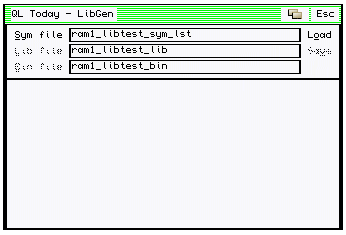
\includegraphics[width=0.65\textwidth]{Content/images/libgen_2.png}
\caption{LibGen in Action}
\label{fig:LibGenInAction}
\end{figure}


\section{The Utilities File}

In a few places in the above code, I am making calls to various
    subroutines to copy strings around, add extensions to filenames, writing
    to and getting input from various information windows etc. The following
    code is the `soon to be' library that facilitates those
    subroutines.

The first subroutine is IW\_INPUT which allows
    an information window to be used to accept input from the user.

It works by calling the WMAN\program{WMAN} routine that sets the channel ID to the
    information window in question, then copies the current value of the
    string to be edited to a working buffer. A jump back into WMAN\program{WMAN} is made to
    allow the user to edit the string. The edit may be terminated by Enter,
    ESC, Up arrow or Down arrow.

The QPTR\program{QPTR} documentation states that D0 will be zero if Enter was
    pressed, negative for any errors, and positive in ESC, Up or Down were
    used to terminate the edit. This is not true as there is no code in WMAN\program{WMAN}
    that does this. D0 will always be zero at the end of an edit, unless any
    errors occurred.

This routine attempts to follow the documentation and does set D0 to
    a positive value -{} it happens to be 1 -{} if the edit ended with a non-{}Enter
    character used to terminate it.

\begin{lstlisting}[firstnumber=1,caption={QlToday\_pe\_utilities\_asm}]
;=====================================================================
; This file contains useful utilities for a Pointer Environment
; application. It's just crying out to become a library! ;-)
;---------------------------------------------------------------------
; IW_INPUT  - Get input from a designated information window.
; IW_PRINT  - Print a string to a designated information window.
; CP_STRING - Copy a string between two locations.
; AP_STRING - Append one string to the end of another.
;=====================================================================


;=====================================================================
; IW_INPUT : accept input from an information window. The routine has
;            a working buffer of 1024 characters maximum which is
;            more than enough for any information window width.
;=====================================================================
; Entry Registers:
;
; D1.W Information window number.
; D2.L Ink colour, or negative ink colour. See WM_SWINF documentation.
; A2.L WMAN vector.
; A3.L Pointer to string.
; A4.L Pointer to work def.
;---------------------------------------------------------------------
; Exit Registers:
;
; D1.W Terminating character: Enter, Esc, Up arrow, Down arrow.
; D2.L Preserved.
; A1.L Buffer pointer.
; A2.L Preserved.
; A3.L Buffer pointer.
; A4.L Preserved.
;---------------------------------------------------------------------
; Errors:
;
; D0 = negative: Any I/O error. Old string unaffected.
; D0 = zero:     Enter terminated the edit. Old string updated.
; D0 = Positive: Another key terminated the edit. Old string updated
;                unless ESC pressed to terminate the edit.
;=====================================================================
iw_input movem.l a2-a3,-(a7)     ; Save WMAN vector & source buffer

iw_copy  lea iw_buffer,a2        ; Copy destination buffer
         bsr cp_string           ; Copy to work buffer
         move.l (a7),a2          ; Get WMAN vector

         jsr wm_swinf(a2)        ; Set channel to info window
         bne.s iw_exit           ; Bale out on error

         lea iw_buffer,a1        ; Edit buffer required in A1
         jsr wm_ename(a2)        ; Edit string in info window
         blt.s iw_exit           ; Negative is an error

;---------------------------------------------------------------------
; Bug alert. It seems at present, that this vector always returns with
; D0 set to zero or negative, but never positive. Sigh. The following
; code tries to reset that situation to how it should be, according to
; the docs.
;---------------------------------------------------------------------

         cmpi.w #27,d1           ; ESC pressed = abort edit
         beq.s iw_esc            ; Yes, all done

         move.l a3,a2            ; Original buffer is destination now
         lea iw_buffer,a3        ; New string found here
         bsr cp_string           ; Copy new value to old buffer

         cmpi.w #$0a,d1          ; Was ENTER pressed to end the edit?
         bne.s iw_esc            ; No, set D0 positive
         clr.l d0                ; Zero = ENTER was pressed
         bra.s iw_exit           ; Done

iw_esc   moveq #1,d0             ; Set D0 positive as required

iw_exit  movem.l (a7)+,a2-a3     ; Tidy WMAN vector off stack
         tst.l d0                ; Because ESC sets Z flag
         rts

;---------------------------------------------------------------------
; Working buffer for IW_INPUT.
;---------------------------------------------------------------------
iw_buffer ds.w 512+1
\end{lstlisting}

The following code prints a string to an information window. The
    information window is cleared first before printing. All the hard work is
    done by WMAN\program{WMAN}.

\begin{lstlisting}[firstnumber=last,caption={QlToday\_pe\_utilities\_asm}]
;=====================================================================
; IW_PRINT : Print a string to a designated information window.
;=====================================================================
; Entry Registers:
;
; D1.W Information window number.
; D2.L Ink colour or negative ink colour. See WM.SWINF documentation.
; A2.L WMAN vector.
; A3.L Pointer to string to be printed.
; A4.L Pointer to window working definition.
;---------------------------------------------------------------------
; Exit Registers:
;
; All registers are preserved except D0.
;---------------------------------------------------------------------
; Errors:
;
; Any I/O error.
;=====================================================================
iw_print movem.l d1-d3/a0-a1/a3,-(a7) ; Save working regsiters
         jsr wm_swinf(a2)        ; Set channel to info window
         bne.s iwp_exit          ; Bale out on error

iwp_cls  moveq #$20,d0           ; CLS
         moveq #-1,d3            ; Timeout
         trap #3                 ; Do it

iwp_prnt moveq #io_sstrg,d0      ; Send a string of bytes
         move.w (a3)+,d2         ; Byte count
         beq.s iwp_exit          ; Nothing to do
         moveq #-1,d3            ; Timeout
         exg a3,a1               ; Pointer in A1 is needed
         trap #3

iwp_exit movem.l (a7)+,d1-d3/a0-a1/a3 Restore working registers
         tst.l d0
         rts
\end{lstlisting}

The subroutine below copies a string from a location pointed to by
    A3 to the location pointed to by A2. The two locations must be holding a
    QDOS formatted string with the word count at the beginning and the bytes
    immediately following.

The code below copies byte by byte so it best suited to fairly small
    strings.

\begin{lstlisting}[firstnumber=last,caption={QlToday\_pe\_utilities\_asm}]
;=====================================================================
; CP_STRING : Copy a string from a buffer at A3.L to a buffer at A2.L.
;             The word length is always copied, even if zero.
;=====================================================================
; Entry Registers:
;
; A2.L Destination buffer address.
; A3.L Source buffer address.
;---------------------------------------------------------------------
; Exit Registers:
:
; All registers, except D0, are preserved.
;---------------------------------------------------------------------
; Errors:
;
; None. D0 is zero on exit.
;=====================================================================
cp_string
         movem.l a2-a3,-(a7)     ; Save the workers
         move.w (a3)+,d0         ; Get the source length
         move.w d0,(a2)+         ; Copy to output buffer
         beq.s cs_exit           ; Nothing more to do

         bra.s cs_next

cs_loop  move.b (a3)+,(a2)+      ; Copy one byte
cs_next  dbf d0,cs_loop          ; And all the rest

cs_exit  movem.l (a7)+,a2-a3     ; Restore the workers
         clr.l d0                ; No errors
         rts
\end{lstlisting}

And finally, for now at least, the last routine in my library (to
    be!) appends the string at A3 to the end of the string at A2. It is the
    responsibility of the programmer to ensure that enough space exists at the
    end of the destination string to hold the string being appended. The
    routine cannot check for this and assumes all will be well.

If your buffer is too small, there is a good chance that whatever
    follows the buffer will be corrupted. You have been warned!

\begin{lstlisting}[firstnumber=last,caption={QlToday\_pe\_utilities\_asm}]
;=====================================================================
; AP_STRING : Append one string to another. The destination buffer is
;             assumed to be big enough for both strings. This code
;             cannot check for this.
;=====================================================================
; Entry Registers:
;
; A2.L Destination string address.
; A3.L String to be added to A2.
;---------------------------------------------------------------------
; Exit Resisters:
;
; All regsiters, except D0, are preserved.
;---------------------------------------------------------------------
; Errors:
;
; None. D0 is zero on exit
;---------------------------------------------------------------------
ap_string
         movem.l d1/a2-a3,-(a7)  ; Save working registers
         move.w (a3)+,d0         ; Get second string size
         beq.s as_exit           ; Nothing to do, bale out

         move.w (a2),d1          ; Current length of destination
         add.w d0,(a2)+          ; Store the new length
         adda.w d1,a2            ; End of destination string
         bra.s as_next

as_loop  move.b (a3)+,(a2)+      ; Append one byte
as_next  dbf d0,as_loop          ; And all the rest

as_exit  movem.l (a7)+,d1/a2-a3  ; Restore working registers
         clr.l d0                ; No errors
         rts
\end{lstlisting}

\section{Possible Enhancements}

The program is complete and working fine as it is, however, there
    are a few enhancements that you might like to add. These could be:
\begin{itemize}[itemsep=0pt]

\item{}Add the ability to put the program to sleep. The code to do this
        is about as simple as it can be and was documented in a past article
        entitled \emph{Easy PEasy Part 2}. Failing this, you can
        examine George's EX0 example from the Easy
        PEasy\program{EasyPEasy} download.


\item{}Improve the error trapping when processing the symbol filename.
        Make sure that the correct extension is present before removing it,
        etc.


\item{}Add a loose item to close the symbol file. When closed the
        screen would be reset to its startup state and the menu removed from
        the application sub-{}window. If you do decide to attempt this, it could
        be worth waiting for the next part as you have nothing to close. But
        you could get it to clear everything out to default for now.


\item{}And anything else you may wish to add yourself.

\end{itemize}

\section{Coming Up...}
\label{ch31-the-end}%\hyperlabel{ch31-the-end}%

So, that's the end of the first part of creating a potentially
    useful utility running under the Pointer Environment. The next chapter 
    will continue from where we left off and add the rest of the
    processing.



%<<<<< YOU ARE HERE >>>>>
%\chapterimage{chapter_head_1.pdf} % Chapter heading image
%\chapter{LibGen -{} Library Generator -{} Parts 2 \& 3}

\section{Introduction}
\label{ch32-intro}%\hyperlabel{ch32-intro}%

\begin{note}
This chapter was originally submitted as one article. Due to space
      restrictions in QL Today, Geoff and Jochen had to split it into two.
      They appeared in Volume 17 issues 1 and 2. Hence the somewhat strange title here!

The corrections posted in the next chapter have been applied to
      this one. Obviously, I couldn't get Jochen to reprint all the affected
      QL Today magazines, so I have been able to correct them here. You know
      what I mean!
\end{note}

\section{LibGen Processing}
\label{ch32-lib-gen-processing}%\hyperlabel{ch32-lib-gen-processing}%

The code for LibGen\program{LibGen}  \emph{should} work as follows:
\begin{enumerate}
\item{The program starts with only the `Esc', `Move' and `Sym file'
        loose items enabled. Everything else is unavailable.
}
\item{The user hits `Sym file'. This causes all loose items except
        `Move' and `Esc' are set to unavailable -{} in case the edit is aborted,
        or an error occurs. The user then types in the name of the sym\_lst
        file created by George's sym\_bin utility.
        The user then terminates or aborts the edit.

On a successful edit, the affected loose items are made
        available again (except `Save'). On an aborted edit, or error, the
        loose items are left unavailable, except for `Sym file' which is reset
        to available. The user will remain at this step until a successful
        edit completes.
}
\item{The `Sym file' name entered by the user is changed by removing
        the `\_sym\_lst' extension and adding `\_lib' in its place to form the
        `Lib file' default file name, and by having the extension `\_bin' added
        on to form the `Bin file' default value. These defaults are displayed
        in the appropriate information windows.
}
\item{When a suitable symbol file name has been entered, all the
        application specific loose items will be enabled with the exception of
        `Save'. The user may use the `Lib file' and `Bin file' loose items to
        amend the default file names for the two files that will be created by
 LibGen on hitting `Save'.
}
\item{When the user hits the `Load', the `Sym file' is opened and read
        in two passes. The first counts the number of \emph{code offset
 }lines that will be added to the menu. The second pass will
        add each one to the buffer allocated, dynamically, for this purpose.
        At end of file, the file will be closed and the buffer added to the
        application sub-{}window as a menu, All items in the menu will be
 \emph{selected} by default. If the file loads correctly,
        the `Save' loose item will be enabled.
}
\item{When the user hits `Save', the currently selected items in the
        application sub-{}window menu will be written out to the `Lib file',
        followed by a command to import the `Bin file'. When complete, the
        file will be closed and all items will be set to the starting position
        where only `Sym file' is available.
}
\end{enumerate}

\section{LibGen Code}

The first version of the code does nothing more than display the
    window on the screen and enter the loop to read the pointer and, as usual,
    this will only return (from WMAN) when an event
    happens or an error occurs in either a loose item hit routine or the
    application menu hit routine. The following code is pretty much a template
    for any
 SETW/EasyPEasy built
    applications. It displays the window on screen and that's about all it
    does -{} pressing the ESC key or HITting/DOing the `Esc' loose item will end
    the program.

\begin{lstlisting}[firstnumber=1,]
         bra   start
         dc.w  0
         dc.w  $4afb

fname    dc.w  fname_e-fname-2
         dc.b  "LibGen - Library Generator"
fname_e  ds.b  0
         ds.w  0

;---------------------------------------------------------------------
; We need the various equates files etc.
;---------------------------------------------------------------------
         in win1_georgegwilt_peass_keys_pe
         in win1_georgegwilt_peass_qdos_pt
         in win1_georgegwilt_peass_keys_wwork
         in win1_georgegwilt_peass_keys_wstatus
         in win1_georgegwilt_peass_keys_wman
         in win1_georgegwilt_peass_keys_wdef

;---------------------------------------------------------------------
; Offsets into the data area for working storage.
;---------------------------------------------------------------------
id       equ 0                   Channel id storage.
wmvec    equ 4                   WMAN vector storage.
slimit   equ 8                   IOP_FLIM output buffer.
\end{lstlisting}

Departing from the template next, I define meaningful names for my
    loose items and information windows. It's much easier to determine which
    loose item or information window is being affected when reading the code
    back in 6 months or so, when you read names as opposed to a list of
    numbers.

I could have simply used an `IN' directive and a separate file at
    this point, which may prove useful for larger applications, but for now,
    I'm simply including the equates directly into my template. You will note
    that the three strings I'm defining storage for are initialised to be zero
    length.

This is important because when we come to allow the user enter the
    symbol filename, the existing string is presented for editing. If we left
    the data uninitialised, we could get some interesting results as random
    strings were presented for editing. It's much better to initialise to an
    empty string as part of the program initialisation.

\begin{lstlisting}[firstnumber=1,]
;---------------------------------------------------------------------
; Loose items we may need.
;---------------------------------------------------------------------
li_symfile equ 2
li_libfile equ 3
li_load    equ 4
li_save    equ 5
li_binfile equ 6

;---------------------------------------------------------------------
; Information windows we may need.
;---------------------------------------------------------------------
iw_symfile equ 2
iw_libfile equ 3
iw_binfile equ 5

;---------------------------------------------------------------------
; Working buffer for the three file names. 40 characters allowed. The
; three strings are initialised to be of zero length.
;---------------------------------------------------------------------

sym_buffer dc.w 0                A zero word count is useful!
           ds.w 20               Space for 40 characters inc N/L.

lib_buffer dc.w 0
           ds.w 20

bin_buffer dc.w 0
           ds.w 20

;---------------------------------------------------------------------
; Buffer for the 2 extra filename extensions we desire. These will be
; added to the end of the supplied sym file name from the user.
;---------------------------------------------------------------------
lib_extn dc.w lib_extn_e-lib_extn-2
         dc.b '_lib'
lib_extn_e equ *

bin_extn dc.w bin_extn_e-bin_extn-2
         dc.b '_bin'
bin_extn_e equ *
\end{lstlisting}

The remainder of the code is back to the template again.

\begin{lstlisting}[firstnumber=1,]
;---------------------------------------------------------------------
; Console definition, and code to open it.
;---------------------------------------------------------------------
con      dc.w con_e-con-2        Size of channel definition.
         dc.b 'con_'
con_e    equ *

op_con   lea  con,a0             We want a console.
         moveq #-1,d1            For this job.
         moveq #0,d3             Timeout.
         moveq #io_open,d0
         trap #2                 Do it.
         rts

;---------------------------------------------------------------------
; The main code itself.
;---------------------------------------------------------------------
start    lea (a6,a4.l),a6        Make A6 point to the job's dataspace.
         bsr op_con              Open a con channel.
         move.l a0,id(a6)        And store the channel id.
         moveq #iop_pinf,d0      Trap to get Pointer Information.
         moveq #-1,d3            Timeout.
         trap #3                 Do it.
         tst.l d0                Is ptr_gen present?
         bne sui                 No, bale out via SUI.
         move.l a1,wmvec(a6)     Yes, store the WMAN vector.
         beq sui                 Oops! WMAN wasn't actually found.

flim     movea.l a1,a2           The WMAN vector is required in A2.
;                                The channel id is already in A0.
         lea slimit(a6),a1       Result buffer.
         moveq #iop_flim,d0      Query maximum size of window.
         moveq #0,d2             D2 is required to be zero.
;                                D3 is the timeout.
         trap #3                 Do it.
         tst.l d0                Did it work?
         bne sui                 No, exit via SUI.

         subi.l #$C0008,(a1)     Minus 12 (width) & 8 (height).
         lea wd0,a3              Get address of window definition.
         move.l #ww0_0,d1        Get size of the working definition.
         bsr getsp               Easy PEasy - ALCHP memory and set A0.
         movea.l a0,a4           Which we save in A4.
         lea wst0,a1             Status area address.
         movea.l a1,a0           Copy to A0.
         moveq #wst0_e-wst0-1,d1 How many bytes to clear - 1.


\end{lstlisting}

So far, we have seen most of this before. However, we depart from
    the normal template in the next few lines, from label
 \texttt{st\_clr} onwards.

\begin{lstlisting}[firstnumber=1,]
st_clr   clr.b (a0)+             Clear one byte.
         dbf d1,st_clr           Then the remainder.

st_loose lea ws_litem+li_libfile(a1),a0  Status byte for Lib file.
         moveq #3,d1             Four status bytes to reset.

st_unav  move.b #wsi_unav,(a0)+  Set loose item to unavailable.
         dbf d1,st_unav          And the rest.
\end{lstlisting}

First we initialise all of the status area, including the loose
    items, to a byte of zero, in the normal manner with the small loop at
 \texttt{st\_clr}. For the loose items, this happens to be the
    status code for available. However, as we don't want every loose item to
    be available when the program starts, the code at
 \texttt{st\_loose} onwards will set the status byte for the 4
    loose items in question, to unavailable -{} there is another way I can set
    these 4 status bytes, as we shall see later on in the code. These will be
    made available by the code in other loose item hit routines as
    appropriate.

I can use a loop at \texttt{st\_unav} because of the
    order I created my loose items in SETW. The 4
    loose items, `Lib file', `Load', `Save' and `Bin file' are set to
    unavailable in this loop. If you created your loose items in a different
    order, you may need to do each one individually.

Because of this status byte being set in the application's
    initialisation, these four loose items will be unavailable when the
    application displays its window on screen.

Back to the template code again.

\begin{lstlisting}[firstnumber=1,]
         movea.l id(a6),a0       Channel ID in A0.
;                                A1 = status area.
;                                A3 = window definition.
;                                A4 = working definition.
         move.l wd_xmin+wd_rbase(a3),d1  Get minimum size.
         andi.l #$FFF0FFF,d1     Mask off scaling factors.
         jsr wm_setup(a2)        Set up the window.

         moveq #-1,d1            Use the current pointer position.
         jsr wm_prpos(a2)        Position as a primary window, then.
         jsr wm_wdraw(a2)        Draw the contents.

;---------------------------------------------------------------------
; The main Read Pointer loop.
;---------------------------------------------------------------------
wrpt     jsr wm_rptr(a2)         Enter read pointer loop in WMAN.
         beq.s no_err            Since D0 is zero D4 is non zero.
         bra sui                 An error occurred exit via SUI.

no_err   movea.l (a4),a1         Status area address.
         btst #pt__can,wsp_weve(a1) Check for CANCEL event.
         bne sui                 Exit.

         bra.s wrpt              No more events, read pointer again.
\end{lstlisting}

I have only included a check for the CANCEL event in the above code.
    Normally there would be SLEEP and SIZE event checking, probably as an
    absolute minimum. However, I need to keep the code size to a minimum for
    the magazine, so these applications will only have the minimum
    required.

Next comes the loose items and application window hit routines. In
    this first version of the code, the loose item hit routines for the
    following 4 loose items simply do nothing except reset the status from
    selected back to available when hit.

\begin{lstlisting}[firstnumber=1,]
;---------------------------------------------------------------------
; Dummy, for now, loose item action routines.
;---------------------------------------------------------------------
afun0_6  bra li_reset            Bin file.
afun0_5  bra li_reset            Save.
afun0_4  bra li_reset            Load.
afun0_3  bra li_reset            Lib file.
afun0_2  bra li_reset            Sym file.
\end{lstlisting}

Before we delve into proper hit routines, the \tablename~\ref{tab:LooseItemHitRoutineRegisters32} is a
    reminder of what registers are set on entry to a loose item hit
    routine.


\begin{table}[htbp]
\centering
\begin{tabular}{l p{0.8\textwidth}}
\toprule
\textbf{Register} &\textbf{Description}  \\
\midrule
%
D1.L & High word = pointer X position, Low Word = pointer Y position.\\
D2.W & Selection keystroke letter, in its upper cased format, or 1 = Hit/SPACE or 2 = DO/ENTER.\\ D2.W & may be an event code if an event triggered this action.\\
D4.B & An event number - if an event triggered this action routine.\\
A0.L & Channel id.\\
A1.L & Pointer to the status area.\\
A2.L & WMAN vector.\\
A3.L & Pointer to loose menu item.\\
A4.L & Pointer to window working definition.\\
%
\bottomrule
\end{tabular}
\caption{Loose Item Hit Routine Registers}
\label{tab:LooseItemHitRoutineRegisters32}
\end{table}

Next up is the first of our working loose item hit routines. This
    one handles the `Move' action. Also showing in the following code is the
    routine where we reset the appropriate loose item's status back to
    available from the currently selected status.

You can see from the above, that the majority of the loose items
    simple reset their status and exit back to
 WMAN.

\begin{lstlisting}[firstnumber=1,]
;---------------------------------------------------------------------
; MOVE hit. Move the window.
;---------------------------------------------------------------------
afun0_1  bsr move


;---------------------------------------------------------------------
; Reset current loose item status to available & redraw. Entry point
; li_reset resets the current loose item while entry at li_rest must
; have a loose item number in D1.W.
;---------------------------------------------------------------------
li_reset move.w wwl_item(a3),d1  Get the loose item number.

li_rest  move.b #wsi_mkav,ws_litem(a1,d1.w) Set status to available.
         moveq #-1,d3            Request selective redraw.
         jsr wm_ldraw(a2)        Do it.
         bra.s li_done
\end{lstlisting}

There are two entry points here, the first at
 \texttt{li\_reset} handles the current loose item. If entry is
    at \texttt{li\_rest} then D1.W should be holding the
    appropriate loose item number.

Within a hit routine, as you may remember, A1 holds the pointer to
    the status area and A3 points at the definition of the loose item within
    the \emph{working definition}. By extracting the loose item
    number from the definition and adding it to A1 plus the offset to the
    start of the status bytes for the loose items, we can change the status to
 \texttt{wsi\_mkav} which is actually the value available +
    redraw.

The code then calls \texttt{wm\_ldraw} to redraw only
    those loose items which have the redraw bit set. This avoids flicker and
    doing unnecessary work redrawing unchanged loose items. When redrawn, the
    redraw bit is cleared by WMAN, leaving the
    status at available.

The code finishes by exiting through \texttt{li\_done} to
    clear out the D0 and D4 registers to indicate no errors and no events.
    After this, it returns back to WMAN and back
    into the pointer loop.

\begin{lstlisting}[firstnumber=1,]
;---------------------------------------------------------------------
; ESC pressed, set cancel event and exit.
;---------------------------------------------------------------------
afun0_0  bset  #pt__can,wsp_weve(a1) Set the CANCEL event bit.
         moveq #pt__can,d4       CANCEL event number in D4.
         bra.s li_exit


li_done  moveq #0,d4             No events.

li_exit  moveq #0,d0             No errors.
         rts                     Exit, and exit from wm_rptr too.



;---------------------------------------------------------------------
; Application sub-window hit routine
;---------------------------------------------------------------------
ahit0    moveq #0,d4             No events.
         moveq #0,d0             No errors.
         rts                     Exit back to the read pointer loop.
\end{lstlisting}

The code that handles a hit on the `Esc' loose item shows the
    alternative manner of handling loose items. It simply sets the CANCEL
    event bit in the event register in the status area (addressed by A1), sets
    the event code in D4 and exits back to WMAN     with D0 set to show no errors.

Having an event code in D4 causes WMAN to
    exit from the pointer reading loop and returns back to
 WMAN with D4 set.
 WMAN will see that an event has been set in D4
    and this will cause a return to our own application code at label
 \texttt{no\_err} (a long way above!). The code there checks for
    the CANCEL event and, if found, exits the program.

\begin{note}
You may be wondering why we gave the ESC loose item a keystroke
      appropriate to the CANCEL event number (3) when we did a little editing
      of the file created by SETW in the last
      article, and why we have to have a loose item hit routine that sets the
      CANCEL event? Surely WMAN handles all
      that?

Well, if you comment out the first two instructions at
 \texttt{afun0\_0} above, reassemble and execute the program
      and then HIT or DO the ESC loose item, you will see it become selected,
      but the program still runs.

However, if you press ESC, WMAN handles
      that and exits from the program. So, we must have the hit routine cause
      the program to exit when the loose item is HIT or DOne because
 WMAN isn't seeing the ESC key being pressed
      to cause an exit. The hit routine for the lose item sets the CANCEL
      event which causes the return to WMAN to
      return to our code and thus, exits from the program. Simple?

Even if there was no loose item to explicitly close the program,
      as long as the application checked for a CANCEL event, as
 LibGen does, we can still close the program
      by pressing the ESC key because WMAN       intercepts the ESC key, generates the CANCEL event and exits back to our
      application code where, hopefully, events are checked for.
\end{note}

Immediately following the `Esc' loose item code we have a dummy
    `does nothing yet' routine for the application window hit routine.

Finally, the last few lines pull in the window definition created by
 SETW and George's
 EasyPEasy library.

\begin{lstlisting}[firstnumber=1,]
;---------------------------------------------------------------------
; Pull in our window definition file.
;---------------------------------------------------------------------

         in  win1_source_qltoday_libgenWin_asm

;---------------------------------------------------------------------
; We need George's Easy PEasy code next.
;---------------------------------------------------------------------

         in  win1_georgegwilt_peass_peas_sym_lst
         lib win1_georgegwilt_peass_peas_bin

;---------------------------------------------------------------------
; And finally, George's sprites.
;---------------------------------------------------------------------

         in  win1_georgegwilt_peass_csprc_sym_lst
         lib win1_georgegwilt_peass_csprc_bin
\end{lstlisting}

If you save and assemble the above, you should be able to execute
    the utility and see it in action. You will only have the `Sym file'
    action, other than move or `Esc' available to you on startup and all the
    filenames will be blank.

At the moment though, even if the `Sym file' loose item is enabled,
    the hit routine does nothing other than set the status back to
    available.

Now that we have the main part of the code to handle the
    initialisation, display and so on working, it's time to add some meat to
    the bones of what we have.

\section{Handling the Sym File Loose Item}
\label{ch32-handling-sym-file}%\hyperlabel{ch32-handling-sym-file}%

Looking back at our LibGen processing
    description above, we have already completed the first step. Step 2
    requires us to let the user type in the symbol file name when the `Sym
    file' loose item is HIT or DOne. Additionally, the `Load' loose item
    becomes available when the action routine completes.

Keeping it simple for now, type in the following code at the
    location of the label \texttt{afun0\_2} which is currently
    showing a branch to the \texttt{li\_reset} routine. The
    following code replaces that which currently exists.

\begin{lstlisting}[firstnumber=1,]
;---------------------------------------------------------------------
; SYM FILE loose item action routine.
;---------------------------------------------------------------------
afun0_2  movem.l d5-d7/a0-a4,-(a7) Preserve important registers.
         bsr sym_hit               Do it all.
         movem.l (a7)+,d5-d7/a0-a4 Restore important registers.
         moveq #li_load,d1       Load loose item.
         bsr li_rest             Make Load available.
         bra li_reset            Make Sym file available.

sym_hit  rts                     Temporary code for now.
\end{lstlisting}

Once again, assemble and execute the code. Now when you HIT or DO
    the `Sym file' loose item, you should see the `Load' loose item become
    available.

The code preserves the registers we need to preserve over an action
    routine, branches out to our temporary hit code and on return, restores
    the registers before setting the `Load' loose item's status byte to
    available. Finally, the code exits via the \texttt{li\_reset}     
    routine which causes the current loose item (`Sym file') to be reset to
    available and redrawn.

That's the easy bit done. The next part gets into the real code for
    a HIT or DO on the `Sym file' loose item. Replace the current one line at
    label \texttt{sym\_hit} with the following code.

\begin{lstlisting}[firstnumber=1,]
;---------------------------------------------------------------------
; This code carries out all the nasty work for a hit on the Sym file
; loose item. It is called from afun0_2 above.
;---------------------------------------------------------------------
sym_hit  moveq #iw_symfile,d1    Info window number in d1.w.
         lea sym_buffer,a3       Current sym file buffer.
         moveq #1,d2             Blue Ink colour.
         bsr iw_input            Get input from desired info window.
         blt.s sh_exit           Something went wrong, bale out.
\end{lstlisting}

It's at this point that having some equates defined for the various
    information windows comes in handy. The code above starts off by loading
    D1 with the number of the information window that will eventually allow us
    to type in the file name and which will also display the file name when we
    have typed it.

A3 holds the address of a buffer, which we set up way back at the
    start. On the first run of the program, this buffer holds a zero length
    string. After it has been run and used, whatever the last symbol file name
    that you typed in will be there.

D2 needs to hold the ink colour, blue in this case, as we will be
    clearing the information window shortly. The code is written so that when
    any information window is being used to edit data, the ink colour is blue,
    but when the data has been entered, it is printed with black ink.

We then branch off to a subroutine names
 \texttt{iw\_input} to allow the user the ability to type in a
    file name directly into the appropriate information window. This routine
    will be discussed later.

On return, if any errors were detected, we bale out. The calling
    code can handle this, as desired. In this example,
 LibGen does nothing with errors. The program
    continues to run, in this case, and you can try again, if desired.

\begin{lstlisting}[firstnumber=1,]
;---------------------------------------------------------------------
; Did we abort the edit?
;---------------------------------------------------------------------
sh_esc   cmpi.w #27,d1           ESC?
         beq.s sh_sym            Yes.
\end{lstlisting}

The \texttt{iw\_input} routine sets the terminating
    character in D1. This can be ESC, ENTER or the Up or Down Arrows. We are
    interested only in the ESC key as this implies that the user decided to
    abort the edit.

If we find the ESC key terminated the edit, we bale out via the
 \texttt{sh\_sym} label, which tidies up the potential garbage
    that is now showing in the information window. The code at
 \texttt{sh\_sym} also prints the file name in black ink as
    opposed to the editing colour of blue.

If the user terminated the edit normally, we have completed step 2
    in our LibGen processing and are ready to carry
    out step 3. The following code does exactly that.

\begin{lstlisting}[firstnumber=1,]
;---------------------------------------------------------------------
; Copy sym filename to other buffers and add appropriate extensions.
; The sym file is assumed to have a '_sym_lst' extension present.
;---------------------------------------------------------------------
sh_ok    move.l a2,-(a7)         Preserve WMAN vector.

         lea lib_buffer,a2       Destination buffer.
         lea sym_buffer,a3       Source buffer.
         bsr cp_string           Copy to lib file.
         subi.w #8,(a2)          Strip off '_sym_lst'.
         bcs.s sh_err            Negative is bad!
         lea lib_extn,a3         Lib file extension.
         bsr ap_string           Add lib file extension.

         lea bin_buffer,a2       Destination buffer.
         lea sym_buffer,a3       Source buffer.
         bsr cp_string           Copy to bin file.
         subi.w #8,(a2)          Strip off '_sym_lst'.
         bcs.s sh_err            Negative is bad!
         lea bin_extn,a3         Bin file extension.
         bsr ap_string           Add it to the bin file.

         moveq #0,d2             Black ink required for filenames.
         move.l (a7)+,a2         Restore WMAN vector.
         moveq #iw_libfile,d1    Info window required.
         lea lib_buffer,a3       String address.
         bsr iw_print            Print lib file.

         moveq #iw_binfile,d1    Info window.
         lea bin_buffer,a3       String address.
         bsr iw_print            Print bin file.
         bra.s sh_sym            Skip error handling.

;---------------------------------------------------------------------
; If the lib or bin filename lengths go negative after subtracting the
; 8 bytes necessary for the assumed '_sym_lst' extension, we bale out
; but need to tidy the stack first.
;---------------------------------------------------------------------
sh_err   move.l (a7)+,a2         Get the WMAN vector again.

\end{lstlisting}

The code above simply copies the file name entered by the user from
    the input buffer to the buffers set aside for the `Lib file' and `Bin
    file'. For each of these, the `\_sym\_lst' extension is removed and a new
    extension appropriate to the file name being generated is appended.

\begin{note}
You will note that there is not much in the way of error trapping
      going on here. This is, again, to keep code to a minimum. A proper
      application would do various checks to ensure that the symbol file
      actually existed, that it had the correct extension and so on, before
      manipulating the file name to create the defaults for the other two file
      names.

The only error trapping that is happening is a check that when
      subtracting 8 from the string length -{} to remove the characters
      `\_sym\_lst' -{} that the string length doesn't go negative. If it does, we
      bale out via \texttt{sh\_err} and \texttt{sh\_sym}       where we tidy up the display again.
\end{note}

The strings are moved around and appended to using some more useful
    routines in one of my libraries. These will be discussed later.

Finally, for this action routine, we have the following code which
    calls yet another of my library routines, \texttt{iw\_print},
    to clear the information window in question, and print the contents of the
    correct buffer to it.

\begin{lstlisting}[firstnumber=1,]
;---------------------------------------------------------------------
; Print the sym file name. We do this at the end of a normal edit and
; when the user aborts with ESC. This keeps the info window tidy.
;---------------------------------------------------------------------
sh_sym   move.w d1,-(a7)         Preserve the terminator keypress
         moveq #iw_symfile,d1    Information window desired.
         moveq #0,d2             Black ink.
         lea sym_buffer,a3       Filename to print.
         bsr iw_print            Print it.
         move.w (a7)+,d1         Restore the termintor keypress

sh_exit  rts
\end{lstlisting}

Unfortunately, at this point, if you assemble the code, you will see
    8 errors. All caused by a lack of my own library routines. The next
    section holds the code for the routines we are using, but have not yet
    created.

\section{The Utilities Library}
\label{ch32-utilities-library}%\hyperlabel{ch32-utilities-library}%

Scroll to the end of the file and add the following lines,
    obviously, you will adjust the file name to suit your own installation.
    Unless, of course, your setup is exactly the same as mine.

You may also note, that while I refer to the code as a library, it
    is not yet converted into one. When we complete
 LibGen, we shall use it to build a working
    library. (Does that count as recursion?)

\begin{lstlisting}[firstnumber=1,]
;---------------------------------------------------------------------
; And finally finally, my own utilities.
;---------------------------------------------------------------------

         in win1_source_qltoday_pe_utilities_asm
\end{lstlisting}

The code above goes just after the part where we pull in George's
    sprite code.

It is not possible for a reusable library's routines to make any
    assumptions about the use of registers outside of the library itself. To
    this end, each of the following routines will preserve any register that
    it uses, with the exception of registers that are documented to return a
    potentially useful value.

Create a new file with the name given above, in my case -{} yours may
    be different, and add the following routines to it.

The first subroutine is \texttt{IW\_INPUT} which allows
    an information window to be used to accept input from the user.

It works by calling the WMAN routine that
    sets the channel ID to the information window in question, then copies the
    current value of the string to be edited to a working buffer. A jump back
    into WMAN is made to allow the user to edit the
    string. The edit may be terminated by ENTER, ESC, Up arrow or Down
    arrow.

\begin{note}
The QPTR documentation states that the \emph{Condition
      Codes}, not D0, will be zero if ENTER was pressed, negative
      for any errors, and positive if ESC, Up or Down were used to terminate
      the edit. D0 will \emph{always} be zero at the end of an
      edit, unless any errors occurred whereupon, it will be negative.

The library routine \texttt{iw\_input} sets D0 to a
      positive value -{} actually 1 -{} when ESC, Up or Down arrow terminates the
      edit.
\end{note}

\begin{lstlisting}[firstnumber=1,]
;=====================================================================
; This file contains useful utilities for a Pointer Environment
; application. It's just crying out to become a library! ;-)
;---------------------------------------------------------------------
; IW_INPUT  - Get input from a designated information window.
; IW_PRINT  - Print a string to a designated information window.
; CP_STRING - Copy a string between two locations.
; AP_STRING - Append one string to the end of another.
;=====================================================================


;=====================================================================
; IW_INPUT : accept input from an information window. The routine has
;            a working buffer of 1024 characters maximum which is
;            more than enough for any information window width.
;=====================================================================
; Entry Registers:
;
; D1.W Information window number.
; D2.L Ink colour, or negative ink colour. See WM_SWINF documentation.
; A2.L WMAN vector.
; A3.L Pointer to string.
; A4.L Pointer to work def.
;---------------------------------------------------------------------
; Exit Registers:
;
; D1.W Terminating character: Enter, Esc, Up arrow, Down arrow.
; D2.L Preserved.
; A1.L Buffer pointer.
; A2.L Preserved.
; A3.L Buffer pointer.
; A4.L Preserved.
;---------------------------------------------------------------------
; Errors:
;
; D0 = negative: Any I/O error. Old string at (A3) unaffected.
; D0 = zero:     Enter terminated the edit. Old string at (A3) updated.
; D0 = Positive: Up, Down or ESC terminated the edit. Old string at (A3)
;                updated, unless ESC pressed.
;=====================================================================
iw_input movem.l a2-a3,-(a7)     Save WMAN vector & source buffer.

iw_copy  lea iw_buffer,a2        Copy destination buffer.
         bsr cp_string           Copy to work buffer.
         move.l (a7),a2          Get WMAN vector.

         jsr wm_swinf(a2)        Set channel to info window.
         bne.s iw_exit           Bale out on error.

         lea iw_buffer,a1        Edit buffer required in A1.
         jsr wm_ename(a2)        Edit string in info window.
         blt.s iw_exit           Negative is an error.

;---------------------------------------------------------------------
; Bug alert. It seems at present, that this vector always returns with
; D0 set to zero or negative, but never positive. Sigh. The following
; code tries to reset that situation to how it should be, according to
; the docs.
; UPDATE: The docs state that it is the CONDITION CODES that return as
; negative, zero or positive and not DO. My code sets D0 as per the 
; condition codes. The manual is actually misleading!
;---------------------------------------------------------------------

         cmpi.w #27,d1           ESC pressed = abort edit.
         beq.s iw_esc            Yes, all done.

         move.l a3,a2            Original buffer is destination now.
         lea iw_buffer,a3        New string found here.
         bsr cp_string           Copy new value to old buffer.

         cmpi.w #$0a,d1          Was ENTER pressed to end the edit?
         bne.s iw_esc            No, set D0 positive.
         clr.l d0                Zero = ENTER was pressed.
         bra.s iw_exit           Done.

iw_esc   moveq #1,d0             Set D0 positive as required.

iw_exit  movem.l (a7)+,a2-a3     Tidy WMAN vector off stack.
         tst.l d0                Make sure Z flag is correct.
         rts

;---------------------------------------------------------------------
; Working buffer for IW_INPUT. A maximum of 1024 characters is allowed.
;---------------------------------------------------------------------
iw_buffer ds.w 512+1
\end{lstlisting}

The next routine is \texttt{iw\_print} and simply prints
    a string to an information window. The information window is cleared first
    before printing. All the hard work is done by
 WMAN.

\begin{lstlisting}[firstnumber=1,]
;=====================================================================
; IW_PRINT : Print a string to a designated information window.
;=====================================================================
; Entry Registers:
;
; D1.W Information window number.
; D2.L Ink colour or negative ink colour. See WM.SWINF documentation.
; A2.L WMAN vector.
; A3.L Pointer to string to be printed.
; A4.L Pointer to window working definition.
;---------------------------------------------------------------------
; Exit Registers:
;
; All registers are preserved except D0.
;---------------------------------------------------------------------
; Errors:
;
; Any I/O error.
;=====================================================================
iw_print movem.l d1-d3/a0-a1/a3,-(a7) Save working regsiters.
         jsr wm_swinf(a2)        Set channel to info window.
         bne.s iwp_exit          Bale out on error.

iwp_cls  moveq #$20,d0           CLS.
         moveq #-1,d3            Timeout.
         trap #3                 Do it.

iwp_prnt move.w (a3)+,d2         Byte count.
         beq.s iwp_exit          Nothing to do.
         moveq #io_sstrg,d0      Send a string of bytes.
         moveq #-1,d3            Timeout.
         exg a3,a1               Pointer in A1 is needed.
         trap #3

iwp_exit movem.l (a7)+,d1-d3/a0-a1/a3 Restore working registers.
         tst.l d0
         rts
\end{lstlisting}

The subroutine \texttt{cp\_string} copies a string from a
    location pointed to by A3 to the location pointed to by A2. The two
    locations must be holding a QDOS formatted string with the word count at
    the beginning and the bytes immediately following.

The code below copies byte by byte so it best suited to fairly small
    strings and no checks are carried out to see if the strings overlap in
    memory, which could lead to corruption after the copy has completed.
    However, it is unlikely for this to actually happen when copying strings
    around.

\begin{lstlisting}[firstnumber=1,]
;=====================================================================
; CP_STRING : Copy a string from a buffer at A3.L to a buffer at A2.L.
;             The word length is always copied, even if zero.
;             NOTE: No checks are done to prevent overlapping!
;=====================================================================
; Entry Registers:
;
; A2.L Destination buffer address.
; A3.L Source buffer address.
;---------------------------------------------------------------------
; Exit Registers:
:
; All registers, except D0, are preserved.
;---------------------------------------------------------------------
; Errors:
;
; None. D0 is zero on exit.
;=====================================================================
cp_string
         movem.l a2-a3,-(a7)     Save the workers.
         move.w (a3)+,d0         Get the source length.
         move.w d0,(a2)+         Copy to output buffer.
         beq.s cs_exit           Nothing more to do.

         bra.s cs_next

cs_loop  move.b (a3)+,(a2)+      Copy one byte.
cs_next  dbf d0,cs_loop          And all the rest.

cs_exit  movem.l (a7)+,a2-a3     Restore the workers.
         clr.l d0                No errors.
         rts
\end{lstlisting}

And finally, for now at least, the \texttt{ap\_string}     routine appends the string at A3 to the end of the string at A2. It is the
    responsibility of the programmer to ensure that enough space exists at the
    end of the destination string to hold the string being appended. The
    routine cannot check for this and assumes all will be well.

If your buffer is too small, there is a good chance that whatever
    follows the buffer will be corrupted. You have been warned!

\begin{lstlisting}[firstnumber=1,]
;=====================================================================
; AP_STRING : Append one string to another. The destination buffer is
;             assumed to be big enough for both strings. This code
;             cannot check for this.
;=====================================================================
; Entry Registers:
;
; A2.L Destination string address.
; A3.L String to be added to A2.
;---------------------------------------------------------------------
; Exit Resisters:
;
; All regsiters, except D0, are preserved.
;---------------------------------------------------------------------
; Errors:
;
; None. D0 is zero on exit
;---------------------------------------------------------------------
ap_string
         movem.l d1/a2-a3,-(a7)  Save working registers.
         move.w (a3)+,d0         Get second string size.
         beq.s as_exit           Nothing to do, bale out.

         move.w (a2),d1          Current length of destination.
         add.w d0,(a2)+          Store the new length.
         adda.w d1,a2            End of destination string.
         bra.s as_next

as_loop  move.b (a3)+,(a2)+      Append one byte.
as_next  dbf d0,as_loop          And all the rest.

as_exit  movem.l (a7)+,d1/a2-a3  Restore working registers.
         clr.l d0                No errors.
         rts
\end{lstlisting}

For now, those are all you need. Now when you assemble the main
    file, it will hopefully assemble without errors and you will be able to
    run the program.

Once you type in a filename which is longer than 7 characters, you
    will hopefully see it transferred to the library and binary filenames but
    each with a separate extension. Under normal circumstances, these defaults
    will be correct, but you will be given the opportunity to change them when
    the symbol file has been loaded.

In order to load the symbol file, you hit the `Load' loose item, or
    press `O', but at the moment, this loose item is not yet wired in, so does
    nothing. If you have a slow QL, you might see the status change from
    available to selected and back to available again.

Pressing the TAB key forces the pointer to jump into the application
    window, and pressing ESC exits the program. Hopefully it will look
    remarkably similar to the screen shot in \figurename~\ref{fig:HowLibGenCurrentlyLooks}.

\begin{figure}[h]
\center
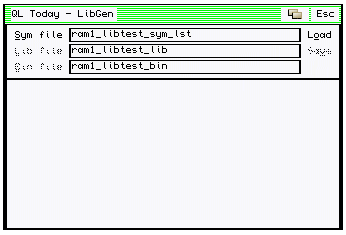
\includegraphics[width=0.65\textwidth]{Content/images/libgen_2.png}
\caption{How LibGen Currently Looks}
\label{fig:HowLibGenCurrentlyLooks}
\end{figure}

%Reference by See \figurename~\ref{fig@YourLabelHere}

We have now almost completed step 3. It is now time to complete step
    3 and move on to step 4. Change the code for the `Sym file' loose item's
    hit routine to the following.

\begin{lstlisting}[firstnumber=1,]
;---------------------------------------------------------------------
; SYM FILE loose item action routine.
;---------------------------------------------------------------------
afun0_2  movem.l d5-d7/a0-a4,-(a7) Preserve important registers.
         bsr.s li_unav           Make LI status unavailable.
         bsr sym_hit             Do it all.
         movem.l (a7)+,d5-d7/a0-a4 Restore important registers.
         cmpi.w #27,d1           Did we abort the edit?
         beq li_reset            Yes, bale out.
         bsr.s li_avail          Make LI status available, if all ok.
         bra li_reset            Make Sym file available.
\end{lstlisting}

The changes are quite simple. We call out to a subroutine -{}
 \texttt{li\_unav} -{} to change the status for all loose items
    from `Lib file' onwards to become unavailable. As we are potentially
    changing the symbol file name in this action routine, we cannot allow
    incorrect data to be used by the Library and Binary file names.

After returning from the main \texttt{sym\_hit} code, we
    check to see if the user aborted the edit with the ESC key. If so, then we
    know that the symbol file name currently on display is potentially
    garbage, and we exit leaving only the `Sym file' loose item
    available.

If the user successfully entered a symbol file name and did not
    abort the edit, we call the routine at \texttt{li\_avail} to
    set all the loose items, except `Save' to available. `Save' will be
    enabled by the actions of the `Load' loose item later.

\begin{lstlisting}[firstnumber=1,]
;---------------------------------------------------------------------
; Reset all Loose Items, affected by hitting "Sym file" to unavailable
; WSI_MKUN = $11 if you are wondering.
;---------------------------------------------------------------------
li_unav  move.b #wsi_mkun,ws_litem+li_libfile(a1)  Make Libfile unavailable
         move.w #$1111,ws_litem+li_load(a1)        Make Load and Save unavailabe
         move.b #wsi_mkun,ws_litem+li_binfile(a1)  Make Binfile unavailable
         bra.s li_rdrw

;---------------------------------------------------------------------
; Reset all Loose Items, affected by hitting "Sym file" to available
; except "Save". WSI_MKAV = $10 if you are wondering.
;---------------------------------------------------------------------
li_avail move.b #wsi_mkav,ws_litem+li_libfile(a1)  Make Libfile available
         move.b #wsi_mkav,ws_litem+li_load(a1)     Make Load available, Save stays Unavailable
         move.b #wsi_mkav,ws_litem+li_binfile(a1)  Make Binfile available

li_rdrw  moveq #-1,d3
         jmp wm_ldraw(a2) 
\end{lstlisting}

The above code is all that is required to enable and disable the
    affected loose items. It is quite simple to do this as there are only 4
    loose items affected and the status bytes for those four are consecutive
    in the status area. Also, for efficiency, we set all 4 as desired, and
    make one single call to \texttt{wm\_ldraw} rather than one call
    per loose item.

\begin{note}
You may remember that I mentioned, way back at the start, that
      there was more than one way to set the status bytes for these 4 loose
      items? Well, the code above is the other way. On a QPC or other device,
      running a 68000 or higher processor, I could have just used a MOVE.L
      \$11111111, WS\_LITEM+LI\_LIBFILE(A1) instruction as the make unavailable
      code. However, because li\_libfile is an odd number, that causes an
      address exception on the 68008 and 68010 processors. The standard QL has
      a 68008 of course.

The above code did in fact use the instruction mentioned. And it
      worked perfectly on my QPC which emulates a 68020, but, as noted in
 Section~\ref{ch33-errata}, this will fail miserably on a standard
      QL so this code is changed from that which first appeared in QL
      Today.
\end{note}

If you now assemble and run the application, HIT `Sym file' and type
    something in. If you abort the edit with ESC then the loose items remain
    disabled. If you press ENTER (or up/down arrows) then the loose items are
    enabled. `Save' remains disabled at all times.

\section{Handling the Lib File Loose Item}
\label{ch32-handling-lib-file}%\hyperlabel{ch32-handling-lib-file}%

There's not much happens when the user HITs the `Lib file' loose
    item. The user is allowed to change the default name, chosen for the
    library file, from that defaulted by LibGen.
    The defaults for this option and the binary file are based on the original
    symbol file which itself is based on the original source file name.

For example, if you assemble a source file named
 \nolinkurl{ram1_libtest_asm}, you will get a generated binary
    file of \nolinkurl{ram1_libtest_bin}, a listing of the code in
 \nolinkurl{ram1_libtest_lst} and a symbol file of
 \nolinkurl{ram1_libtest_sym}.

Using George's sym\_bin utility, you
    convert \nolinkurl{ram1_libtest_sym} into
 \nolinkurl{ram1_libtest_sym_lst}. It is this latter file that
 LibGen processes for you.

Based on the name of this latter file, LibGen chooses
 \nolinkurl{ram1_libtest_lib} for the library file -{} the one
    containing an `IN' and a `BIN' instruction, and for the actual binary file
    making up the library, chooses
 \nolinkurl{ram1_libtest_bin}.

In most cases, these defaults will be fine, but at least
 LibGen gives you the ability to change them as
    desired. After all, it's not wise to keep your various library files on
 \nolinkurl{ram1_} is it!

The code for the `Lib file' hit routine is as follows. This replaces
    the existing dummy code already in the main source file.

\begin{lstlisting}[firstnumber=1,]
;---------------------------------------------------------------------
; LIB FILE loose item action routine.
;---------------------------------------------------------------------
afun0_3  movem.l d5-d7/a0-a4,-(a7) Preserve important registers.
         bsr lib_hit             Do it all.
         movem.l (a7)+,d5-d7/a0-a4 Restore important registers.
         bra li_reset            Make Lib file available.
\end{lstlisting}

As before, I tend to prefer the actual hit routine to be small. The
    above code simply preserves the desired registers, calls out to the
 \texttt{lib\_hit} code, then restores the registers and exits
    resetting the `Lib file' loose item to available. You will see that it
    remains in a selected state until you complete the edit.

\begin{lstlisting}[firstnumber=1,]
;---------------------------------------------------------------------
; This code carries out all the nasty work for a hit on the Lib file
; loose item. It is called from afun0_3 above.
;---------------------------------------------------------------------
lib_hit  moveq #iw_libfile,d1    Info window number in d1.w.
         lea lib_buffer,a3       Current lib file buffer.
         moveq #1,d2             Blue Ink when editing.
         bsr iw_input            Get input from desired info window.
         bmi.s lf_exit           Something went wrong, bale out.
\end{lstlisting}

Nothing much of interest here, the processing is almost identical to
    that we have seen already for allowing the user the ability to type a
    symbol file name. We don't have to check for the ESC key terminating the
    edit because we always, unless there was an error, exit via the tidy up
    code at \texttt{lf\_ok}. Remember that our library routine
 \texttt{iw\_input} copies the data from the working edit buffer
    back to the correct location on a successful edit.

\begin{lstlisting}[firstnumber=1,]
;---------------------------------------------------------------------
; Print the lib file name. We do this at the end of a normal edit and
; when the user aborts with ESC. This keeps the info window tidy.
;---------------------------------------------------------------------
lf_ok    moveq #iw_libfile,d1    Information window desired.
         moveq #0,d2             Black ink.
         lea lib_buffer,a3       Filename to print.
         bsr iw_print            Print it.
         
lf_exit rts 
\end{lstlisting}

The code above, you may notice, doesn't preserve the terminating
    character in D1. There isn't really any requirement to do so in the
    handling of a `Lib file' HIT.

\section{Handling the Bin File Loose Item}
\label{ch32-handling-bin-file}%\hyperlabel{ch32-handling-bin-file}%

The code for handling a hit on the `Bin file' loose item is almost
    identical to the above. It will be shown here without further
    discussion.

\begin{lstlisting}[firstnumber=1,]
;---------------------------------------------------------------------
; BIN FILE loose item action routine.
;---------------------------------------------------------------------
afun0_6  movem.l d5-d7/a0-a4,-(a7) Preserve important registers.
         bsr bin_hit             Do it all.
         movem.l (a7)+,d5-d7/a0-a4 Restore important registers.
         bra li_reset            Make Bin file available.

;---------------------------------------------------------------------
; This code carries out all the nasty work for a hit on the Bin file
; loose item. It is called from afun0_6 above.
;---------------------------------------------------------------------
bin_hit  moveq #iw_binfile,d1    Info window number in d1.w.
         lea bin_buffer,a3       Current bin file buffer.
         moveq #1,d2             Blue ink when editing.
         bsr iw_input            Get input from desired info window.
         bmi.s bf_exit           Something went wrong, bale out.

;---------------------------------------------------------------------
; Print the bin file name. We do this at the end of a normal edit and
; when the user aborts with ESC. This keeps the info window tidy.
;---------------------------------------------------------------------
bf_ok    moveq #iw_binfile,d1    Information window desired.
         moveq #0,d2             Black ink.
         lea bin_buffer,a3       Filename to print.
         bsr iw_print            Print it.
         
bf_exit rts 
\end{lstlisting}

If you assemble the code and execute it you should find that
    everything works as desired.

\section{Coming Up...}
\label{ch32-the-end}%\hyperlabel{ch32-the-end}%

In the next chapter we will add the real meat of
    the utility -{} the ability to load a file, select which entries you want
    from a menu, and then save those entries out to a file suitable for
    inclusion in future assembly programs.


%\chapterimage{chapter_head_2.pdf} % Chapter heading image
%\chapter{LibGen -{} Library Generator -{} Part 4}

\section{Introduction}
\label{ch33-intro}%\hyperlabel{ch33-intro}%

In the previous chapter, we ended up with an application that was getting
    somewhere. But it's not finished yet. This issue we will look at what
    happens when the user requests that we load a symbol file. In this
    article, as before, we shall add code gradually, starting simple and
    getting more complicated as we go on.

\section{Gwasl Update}
\label{ch33-gwasl-update}%\hyperlabel{ch33-gwasl-update}%

George has updated gwasl to version 2.05
    to fix a slight bug in error handling. To be sure you have the latest
    version, please download it from \href{http://gwiltprogs.info/gwaslp08.zip}{http://gwiltprogs.info/\-gwaslp08.zip}.
    We will be using this version from now on.

\section{Errata}
\label{ch33-errata}%\hyperlabel{ch33-errata}%

In the previous edition, Volume 17 Issue 2 dated December 2012 to
    February 2013, George Gwilt spotted a couple of errors in my code.

In the IW\_PRINT sub-{}routine, at label
 IWP\_PRINT, we have the following:

\begin{lstlisting}[firstnumber=1,]
iwp_prnt moveq #io_sstrg,d0
         move.w (a3)+,d2
         beq.s iwp_exit
\end{lstlisting}

The code is incorrect in that it introduces a bug. If there is no
    string to print, the code exits directly to iwp\_exit where D0 is tested
    and the condition codes set. Unfortunately, this means that the condition
    codes will be set to reflect the fact that D0 is currently sitting with
    the value \#IO\_SSTRG and not an error code. This is a bad thing!

The code above must be changed as follows:

\begin{lstlisting}[firstnumber=1,]
iwp_prnt move.w (a3)+,d2
         beq.s iwp_exit
         moveq #io_sstrg,d0
\end{lstlisting}

In this corrected version, D0 will contain zero on return from the
    previous trap and thus, on early exit to IWP\_EXIT,
    the condition codes will be set to reflect this zero value, and the code
    will assume that all is well, which it is. The window has been cleared and
    nothing has been printed -{} which is exactly what is desired.

Also in the sub-{}routine IW\_INPUT, on page 22, I
    have a comment near the bottom of the page that details a bug in the
    documentation for the WM\_ENAME vector. The comment is
    incorrect and should be removed. This has arisen due to a misunderstanding
    of the documentation, on my part.

I assumed that when the docs mentioned that the condition codes
    would be set, that what they really meant was that D0 would be set. A
    completely incorrect assumption on my part. However, I wrote the library
    routine with that assumption in mind. As it turned out, after an exchange
    of emails with George, the manual is correct and I am wrong.

If you leave the code the way it is, D0 will be set to negative,
    zero or positive as I originally misunderstood the manual to say. It does
    no harm, but the comments itself is wrong and should be removed as there
    is not a bug in the manual.

This also means that on page 21, the first line of the note, where
    it says that ``D0 will be zero if ENTER was pressed...to terminate the
    edit.'', it is wrong. That whole paragraph can simply be ignored. Typpex it
    out if you must! ;-{})

My apologies for these problems, and my thanks to George for his
    assistance in resolving my issues.

George also pointed out that in the routines
 CP\_STRING and AP\_STRING, where
    the test for a zero length string is made, it is not necessary as the DBF
    instruction will detect this and do nothing anyway. What George says is
    true, but I tend to like to be explicit in my code. To this end, you can,
    if you wish to save a couple of bytes and clock cycles, remove the BEQ.S
    CS\_EXIT and/or BEQ.S AS\_EXIT instructions from near the start of these
    routines.

George further pointed out my use of the BLT instruction as opposed
    to the BMI command. Once I checked my documentation, I discovered that
    George is correct -{} although the conditions under which BLT wouldn't work
    are unlikely, I have decided to correct the code. There are three
    occasions where the instruction BLT.S xx\_EXIT, where xx is a two letter
    prefix, should be changed to BMI.S xx\_exit instead. They three locations
    are in the routines at SYM\_HIT,
 LIB\_HIT and BIN\_HIT. Please
    change all three BLT instructions to BMI.

What's the difference? Well, my code is looking for a negative
    number, and if found, currently bales out via the BLT instruction. How do
    you determine whether a number is negative or not? The N flag tells you.
    If the N flag is set, the number in question is negative, otherwise, it is
    positive.

The BMI instruction checks the N flag and branches accordingly. The
    BLT instruction, on the other hand, will branch only if the N flag is set
    and the V (overflow) flag is not set, or, if the V flag is set and the N
    flag is not.

And finally, here's a couple I spotted myself. Unfortunately,
    because I'm running on QPC with a virtual) 68020, the following two bugs
    don't cause an exception, however, running on a standard QL, they
    would.

The code at LI\_UNAV and
 LI\_AVAIL currently looks like this:

\begin{lstlisting}[firstnumber=1,]
li_unav  move.l #$11111111,ws_litem+li_libfile(a1)
         bra.s li_rdrw
...
li_avail move.l #$01011101,ws_litem+li_libfile(a1)

li_rdrw  moveq #-1,d3
         jmp wm_ldraw(a2) 
\end{lstlisting}

The problem is, LI\_LIBFILE is an odd value -{} it's \$03. Although A1.L
    and WS\_LITEM are both guaranteed to be even, the effective address of the
    MOVE.L is an odd address. As I mentioned, this works perfectly well on QPC
    with its 68020 processor, but the 68008 in our bare bones QLs will raise
    an address exception. We need to change the code as follows:

\begin{lstlisting}[firstnumber=1,]
li_unav  move.b #wsi_mkun,ws_litem+li_libfile(a1)  Make Libfile unavailable
         move.w #$1111,ws_litem+li_load(a1)        Make Load and Save unavailabe
         move.b #wsi_mkun,ws_litem+li_binfile(a1)  Make Binfile unavailable
         bra.s li_rdrw
...
li_avail move.b #wsi_mkav,ws_litem+li_libfile(a1)  Make Libfile available
         move.b #wsi_mkav,ws_litem+li_load(a1)     Make Load available, Save stays Unavailable
         move.b #wsi_mkav,ws_litem+li_binfile(a1)  Make Binfile available

li_rdrw  moveq #-1,d3
         jmp wm_ldraw(a2) 
\end{lstlisting}

\section{Another Library}
\label{ch33-another-library}%\hyperlabel{ch33-another-library}%

The processing for the Load and Save loose items requires a bit
    of file processing. I have a library for this, as you might expect. So,
    without any further ado, here it is. Mine is called
 \nolinkurl{win1_source_qltoday_openfiles_asm} at the moment, and
    is simply included as a plain source file, it's not a proper library yet.
    If you save your file in a different place, please be sure to change the
    name in the `in' command.

\begin{lstlisting}[firstnumber=1,]
;=====================================================================
; This file contains useful utilities for opening files etc.
; It's just crying out to become a library! ;-)
;---------------------------------------------------------------------
; F_OPEN      - Open a file. Old Exclusive mode.
; F_OPEN_IN   - Open a file for input. Old Shared mode.
; F_OPEN_NEW  - Open a new file. New Exclusive mode.
; F_OPEN_OVER - Open overwrite. New Overwrite mode.
; F_OPEN_DIR  - Open a directory. Open Directory mode.
; F_CLOSE     - Close any open file.
; F_SYNC      - Flush buffers to device.
; F_POS_ABS   - Set absolute file position.
; F_POS_REL   - Set relative file position.
;=====================================================================
; Entry Registers.
;
; Unless otherwise specified, all routines use the following registers
; on entry:
;
; A0.L Pointer to QDOSSMQ string defining the file name.
;---------------------------------------------------------------------
; Exit Registers.
;
; Unless otherwise specified, all routines exit with the following
; register usage. Any register not listed will be preserved by the
; routines.
;
; D0.L Error code. Zero = no errors.
; A0.L Channel id.
; Flags - Z set to reflect the value in D0.
;=====================================================================

io_openx      equ 0   SuperBasic OPEN
io_open_in    equ 1   SuperBasic OPEN_IN
io_open_new   equ 2   SuperBasic OPEN_NEW
io_open_over  equ 3   SuperBasic OPEN_OVER
io_open_dir   equ 4   No SuperBasic equivalent.


;=====================================================================
; F_OPEN - Open an existing file.
;=====================================================================
f_open
        move.l d3,-(a7)        Save D3
        moveq #io_openx,d3     IO Open code
        bra.s f_open_all       Go do it, and exit.


;=====================================================================
; F_OPEN_IN - Open a file for input.
;=====================================================================
f_open_in
        move.l d3,-(a7)
        moveq #io_open_in,d3
        bra.s f_open_all


;=====================================================================
; F_OPEN_NEW - Craete a new file.
;=====================================================================
f_open_new
        move.l d3,-(a7)
        moveq #io_open_new,d3
        bra.s f_open_all


;=====================================================================
; F_OPEN_OVER - Open a file, overwriting existing contents.
;=====================================================================
f_open_over
        move.l d3,-(a7)
        moveq #io_open_over,d3
        bra.s f_open_all


;=====================================================================
; F_OPEN_DIR - Open a device directory.
;=====================================================================
f_open_dir
        move.l d3,-(a7)
        moveq #io_open_dir,d3


;=====================================================================
; F_OPEN_ALL - general purpose working "open" routine.
;=====================================================================
f_open_all
        movem.l d1-d2/a1,-(a7) Save working registers
        moveq #io_open,d0      IO_OPEN trap code
        moveq #-1,d1           File is for this job
;                              D3 already set
;                              A0 already set
        trap #2                Do it
        movem.l (a7)+,d1-d2/a1 Restore working registers
        move.l (a7)+,d3        Plus D3 from above
        tst.l d0               Set Z flag
        rts                    Done
\end{lstlisting}

The first few routines are all to do with opening files. All that
    they do is set the required open mode in D3 then branch down to doing all
    the hard work at f\_open\_all. D3 is also preserved by the individual
    routines as we need to keep it safe from changes.

On arrival at f\_open\_all, we preserve all the
    other working registers and call out to QDOSMSQ to open the file for us.
    On return, A0 holds the channel id and D0 any potential error codes. After
    restoring all the working registers, and D3, we set the flags according to
    D0's error code and exit.

\begin{lstlisting}[firstnumber=1,]
;=====================================================================
; F_CLOSE - Close any open file.
;=====================================================================
; Entry Registers:
;
; A0.L Channel Id
;---------------------------------------------------------------------
; Exit Registers:
;
; D0.L Error code (channel not open)
; A0.L Corrrupted.
; Flags Z set according to D0.
;=====================================================================
f_close
        moveq #io_close,d0     Close file trap code
        trap #2                Do it
        tst.l d0               Set Z flag
        rts                    Done
\end{lstlisting}

The f\_close routine simply closes the channel
    id passed in A0, and returns with any errors in D0 and the Z flag set
    accordingly.

\begin{lstlisting}[firstnumber=1,]
;=====================================================================
; F_POS_ABS - Set the current file position pointer to an absolute
;          position in the file.
;=====================================================================
; Entry Registers:
;
; D1.L File position required.
; A0.L Channel Id.
;---------------------------------------------------------------------
; Exit Registers:
;
; D0.L Error code.
; D1.L New file position.
; Flags Z set according to D0.
;=====================================================================
f_pos_abs
        moveq #fs_posab,d0     Abs position trap code
        bra.s f_pos_all        Do it


;=====================================================================
; F_POS_REL - Set the file position to a new location relative to the
;          current location.
;=====================================================================
; For register usages, see F_POS_ABS above.
;=====================================================================
f_pos_rel
        moveq #fs_posre,d0     Relative position trap code


;=====================================================================
; F_POS_ALL - General do it all file positioning routine.
;=====================================================================
f_pos_all
        movem.l d3/a1,-(a7)    Preserve working registers
        moveq #-1,d3           Timeout
;                              D0 already set to trap code
;                              D1 already set to file location
;                              A0 already set to channel id
        trap #3                Do it
        movem.l (a7)+,d3/a1    Restore registers
        tst.l d0               Set Z flag
        rts                    Done


;=====================================================================
; F_FLUSH - Flush a file's slave blocks to disc.
;=====================================================================
; Entry Registers:
;
; A0.L Channel Id.
;---------------------------------------------------------------------
; Exit Registers:
;
; D0.L Error code.
; Flags Z set according to D0.
;=====================================================================
f_flush
        movem.l d1/d3/a1,-(a7) Preserve working registers
        moveq #fs_flush,d0     Trap code
        moveq #-1,d3           Timeout
;                              A0 already set to channel id
        trap #3                Do it
        movem.l (a7)+,d1/d3/a1 Restore registers
        tst.l d0               Set flags
        rts                    Done
\end{lstlisting}

The above routines carry out useful file flushing and positioning
    facilities. As ever, the channel id is passed in A0, and for the file
    positioning routines, a file location in D1.L. After preserving the
    working registers, the routines simply call out to QDOSMSQ to do the hard
    work before restoring any working registers and exiting with the Z flag
    set according to the error code in D0.

The following one line needs to be added to the end of
 \nolinkurl{libgen_asm} to include the above library of useful
    file handling routines.

\begin{lstlisting}[firstnumber=1,]
         in  win1_source_qltoday_openfiles_asm
\end{lstlisting}

It should be added after the existing line that includes my
 \nolinkurl{pe_utilities_asm} source file.

\section{Load Processing}
\label{ch33-lib-gen-processing}%\hyperlabel{ch33-lib-gen-processing}%

When the user hits the Load loose item, the file named as the
    Symbol file, is opened for reading. It is then processed in two
    passes.

The first pass simply counts the number of \emph{code offset
 }lines that will be added to the menu. This is done by looking
    along the entire line of text read in, for the appearance of the
    characters `*+' as these two indicate that the entry is for a code offset
    rather than an equate. If we find what we are looking for, so we increment
    the counter. Any errors cause an immediate return with the Z flag
    indicating success or failure.

The second pass resets the file position back to the start, and
    begins reading again. This time, for each entry that represents a code
    offset, we extract the label name from the entry, and add it to the buffer
    allocated for the application menu. Again, in the event of an error, we
    return with the Z flag holding the success or failure status.

If all is well, then at end of file, the file will be closed and the
    buffer added to the application sub-{}window as a menu, All items in the
    menu will be \emph{selected} by default. If the file loads
    correctly, the "Save" loose item will be enabled and the Load loose item
    will be reset to available.

I did consider reading the \nolinkurl{_sym} file directly
    and bypassing the need to create a \nolinkurl{_sym_lst} file. I
    got as far as diagnosing the internal structure of a
 gwasl \nolinkurl{_sym} file and even
    worked out a fairly simple manner of processing the load requirements.
    Unfortunately, George advised that I stick with the
 \nolinkurl{_sym_lst} file as it is identical whether the original
 \nolinkurl{_sym} file was created with
 gwasl or gwass -{} as
    these produce a different \nolinkurl{_sym} file format.

I did a quick test using gwass instead of
 gwasl and sure enough, the
 \nolinkurl{_sym} files are different. Equally, the
 \nolinkurl{_sym_lst} files are also different, so I need to scan
    each line read in from the file looking for the special characters I want
    instead of just checking a specific location in the line. Never mind, this
    way, if George changes things, LibGen will
    still work.

\section{LibGen Code}

As with the other hit routines, we start off quite simple. The
    following code is all that is required as the main Load loose item hit
    routine:

\begin{lstlisting}[firstnumber=1,]
;---------------------------------------------------------------------
; LOAD loose item action routine.
;---------------------------------------------------------------------
afun0_4  movem.l d5-d7/a0-a4,-(a7) Preserve important registers.
         bsr load_hit              Do it all.
         movem.l (a7)+,d5-d7/a0-a4 Restore important registers.
         move.w #$0101,ws_litem+li_load(a1) Only works because li_load is even!
         bra li_rdrw               Load = available, Save = available.

;---------------------------------------------------------------------
; This code carries out all the nasty work for a hit on the Load
; loose item. It is called from afun0_4 above.
;---------------------------------------------------------------------
load_hit bsr.s ld_pass_1           Count the entries for the menu
         bne.s ld_exit             Oops, an error occurred
         bsr ld_pass_2             Build the menu
         
ld_exit  rts                       Done, D0 = error or not

;---------------------------------------------------------------------
; Load file, pass 1, open the symbol file and count the code offsets.
;---------------------------------------------------------------------
ld_pass_1
         moveq #0,d0
         rts

;---------------------------------------------------------------------
; Load file, pass 2, build the menu, close the symbol file.
;---------------------------------------------------------------------
ld_pass_2
         moveq #0,d0
         rts
\end{lstlisting}

The main meat of the hit code is yet to be written, however,
    assembling the above and executing it shows that when the Load loose
    item is hit, both it and the Save one become available. Nothing will
    happen if you now hit or do the Save loose item because it still has a
    dummy hit routine that does nothing, other than to reset the loose item to
    available. If you have a slow QL, you might see the Save loose item
    flash as it has its status reset from selected to available.

An important point to note. The setting of the two loose items to
    available by a single MOVE.W instruction only works because ws\_litem is
    defined as even, its value is \$40 and, as I already know that li\_load is
    also even, then the MOVE.W works. If either of these (or for that matter,
    A1) were odd, there would be an address exception on a standard QL, but
    not on QPC. If you ever wish to add extra loose items to this utility, and
    want to be extra safe, then change the single MOVE.W above, to the
    following:

\begin{lstlisting}[firstnumber=1,]
         move.b #wsi_mkav,ws_litem+li_load(a1) Make Load available.
         move.b #wsi_mkav,ws_litem+li_save(a1) Make Save available.
\end{lstlisting}

We need to add a couple of helper routines next, and then, we can
    hook them up to ld\_pass\_1 replace the dummy code we
    have there at present.

As we have to scan each line of the \nolinkurl{_sym_lst}     file for the characters `*+' in both passes, it's probably wise to extract
    the code to a separate sub-{}routine. However, there's a slight problem. In
    the first pass we are simply counting entries so that we can allocate the
    correct amount of memory to build the menu, while in pass 2 we have to
    extract all the names and offsets to actually use in the menu. What to
    do?

The answer is simple, if we set an address register to the address
    of a sub-{}routine to carry out the required work, we can use the JSR (An)
    instruction each time we find the required text. That way, each pass will
    set the register to a different address and whatever code is at that
    address when we find a line containing a code offset, will be executed.
    Simple!

The following code is our equivalent of INSTR. You should type it in
    just above where ld\_pass\_2 is currently
    located.

\begin{lstlisting}[firstnumber=1,]
;=====================================================================
; LD_INSTR - scans each line of the buffer at (A1) looking for the 
;            characters '*+' and if found, calls the code at the 
;            address in A2.
;=====================================================================
; Entry Registers:
;
; A1.L Buffer to search. Normal QDOS format of word and bytes.
; A2.L Address of code to be called on a "find". Zero if nothing.
;---------------------------------------------------------------------
; Exit Registers:
;
; A1.L Address in buffer of the character after the '*' we looked for,
;      if found. Points at the '+'. If not found, one past the buffer
;      end if not found.
;
; D0.L  0 = Found the '*+'.
;      -1 = Not found.
;      -ve = Appropriate error.   
;
; Flags Z set according to D0.
;=====================================================================
ld_instr moveq #0,d0               Need D0.L to be zero
         move.w (a1)+,d0           Grab the word count
         beq.s ldi_done            Unlikely, but you never know!
         bra.s ldi_next            Decrement before comparing

ldi_scan cmpi.b #'*',(a1)+         Compare and increment
ldi_next dbeq d0,ldi_scan          Try again or drop out

;---------------------------------------------------------------------
; If we get here we have either found a '*' or we haven't. If D0.W is
; -1 then we didn't find it. Otherwise the Z flag should be set.
;---------------------------------------------------------------------
         bne.s ldi_exit            Bale out, D0 = -1 = not found
         cmpi.b #'+',(a1)          Compare, but don't increment
         bne.s ldi_next            Keep searching (unlikely!)

;---------------------------------------------------------------------
; Found '*+' if A2 is non-zero, call the code addressed in A2.
;---------------------------------------------------------------------
         cmpa.l #0,a2              Anything to execute?
         beq.s ldi_exit            No, bale out D0 = 0 = found
         jsr (a2)                  Yes, call the code

;---------------------------------------------------------------------
; A not found means we arrive here with D0.W = -1 instead of D0.L. We
; must extend D0.W to a long or the calling code will barf! 
;---------------------------------------------------------------------
ldi_exit ext.l d0                  Must exit with error code in D0.L

ldi_done rts                       Done
\end{lstlisting}

As you can see it's quite simple. We are passed a buffer address in
    A1.L and a code address in A2.L. D0 is set to the word count for the size
    of the data in the buffer, and then we enter a loop to search for the
    required `*' character in the buffer. If we hit the end of the buffer, D0
    will be -{}1 and the Z flag will not be set, so we exit directly to the RTS
    instruction at ldi\_done which means we return -{}1 as a
    flag that we didn't find anything.

Note that in the event that we don't find the `*' we are looking
    for, D0.L holds the value \$0000FFFF. The calling code adds 1 to D0.L to
    determine if it was a not found or some other error, so we have to make
    sure that D0.L holds \$FFFFFFFF.

The code at ldi\_exit does this, but also does
    it when we have found it, whether or not we call any code in A2, so in
    that case, it's an un-{}required instruction. However, it does nicely set
    the flags for us so we don't have to TST.L D0 on the way out.

If we do find an `*' character, we exit from the bottom of the loop
    with the condition codes set to `eq' (the same condition as the 'cc' part
    of the DBcc instruction) so we know we found it. A1.L is pointing at the
    character after the `*' and we hope that it is a `+'. If it is not a plus,
    then we skip back into the loop to see if there are any more `*'
    characters. This is unlikely in a \nolinkurl{_sym_lst} file, but
    you never can be too sure!

Assuming the character at A1.L is a plus, we check if A2.L is zero
    and of so, exit setting D0 to zero to indicate found. If A2.L holds some
    other value, we call the code pointed to by A2.L and, on return, make sure
    the flags are set according to any potential error codes in D0, and
    exit.

We are now ready to write the code to replace the dummy code at
 ld\_pass\_1.

\begin{lstlisting}[firstnumber=1,]
ld_pass_1 
         lea sym_buffer,a0         File name
         bsr f_open_in             File must exist already for reading
         bne sui                   Error exit, dramatic and fatal!

         moveq #0,d7               Counter register
         lea ld_p1_count,a2        Call back code to do the counting

p1_entry moveq #128,d2             Size of buffer space. (Preserved)
         moveq #-1,d3              Timeout (Preserved)
\end{lstlisting}

The main entry point to pass attempts to open the file who's name is
    currently stored in the sym file buffer. If it fails to open for any
    reason, I'm afraid the application simply dies. This is not ideal and in a
    commercia" quality application this would simply be unacceptable. I only
    do it here to reduce space in the magazine.
\begin{DBKadmonition}{}{Note}

I know how irritating it can be for a program to just vanish.
      During testing I had a bug that caused the program to quit whenever a
      line didn't contain an asterisk. The reason was that D0.L held \$0000FFFF
      and not \$FFFFFFFF on exit from ld\_instr.
\end{DBKadmonition}

The next step is to zero D7 which is acting as our counter. The
    whole of D7.L is set to zero although the code only requires the low word.
    A2.L is loaded with the address of the callback routine that does the
    counting for us. Every time there's a hit in the data read from the
 \nolinkurl{_sym_lst} file, we jump to the code whose address is
    held in A2.L. On this pass, it simply counts. (See below.)

P1\_entry is the second entry point to this
    code. There's no point duplicating huge chunks of code, and as pass 1 and
    pass 2 are both required to read the file, and scan each line of text read
    from it, we can use the code in pass 1 as part of pass 2.
 P1\_entry will be where pass 2 joins in with the
    fun.

At this point, we have everything initialised for pass 1. The buffer
    length for IO\_FLINE is set as is the timeout. These two registers are
    preserved through the calls to IO\_FLINE so can be initialised once only,
    prior to the start of the main loop for each pass.

\begin{lstlisting}[firstnumber=1,]
p1_loop  lea p1_buffer+2,a1        We need to reinitialise the each time
;                                  A0.L already has the channel id
;                                  D2.W already has the buffer size
;                                  D3 already holds the timeout
         moveq #io_fline,d0        The trap code we desire
         trap #3                   Read up to 128 bytes ending with a lf
         tst.l d0                  Errors?
         beq.s p1_not_eof          No, all ok, skip

p1_eof   cmpi.l #-10,d0            Was it EOF?
         bne sui                   No, error, die horribly!
         bra.s p1_exit             Must be EOF, all done for pass 1

p1_not_eof
         subq.w #1,d1              Lose the terminating lf character
         beq.s p1_next             Nothing to do here, empty line
         lea p1_buffer,a1          Buffer address again
         move.w d1,(a1)            Make into QDOSMSQ string
\end{lstlisting}

The first part of the main loop sets A1.L to the third character of
    the buffer we will use to read each line of data from the
 \nolinkurl{_sym_lst} file into. IO\_FLINE fetches
 \emph{bytes}, not a QDOSMSQ string with a word count, so we
    cannot simply point A1 at the start of the buffer.

We call IO\_FLINE to read some text up to a maximum of 128 bytes, but
    normally terminating with a linefeed character. On return, if D0.L is EOF,
    we exit as this concludes pass 1. If D0.L is holding any other error code,
    the application simply takes the easy way out and dies horribly.

The number of characters read, including the linefeed is returned in
    D1.W from which, we subtract 1 to lose the trailing linefeed. We skip to
    the end of the loop if the length is now zero as we can't scan an empty
    string. If there is work to do, we reset A1.L to the word count at the
    start of the buffer and store the length word, now not including the
    linefeed. We are now ready to scan the fresh data in the buffer.

\begin{lstlisting}[firstnumber=1,]
         bsr.s ld_instr            Scan for the required characters
         beq.s p1_next             We found it, do next line of data
         addq.l #1,d0              Minus 1 was not found
         bne sui                   Oh dear, some other error. Die

p1_next  bra.s p1_loop             Let's go round again

p1_exit  moveq #0,d0               No errors. We come here from EOF only
         rts
\end{lstlisting}

The above code calls the `instr' code to look for the two desired
    characters. If found, D0.L will be zero on return. In that case, we skip
    to the bottom of the main loop ready to go round again. If D0.Lholds minus
    1 then that indicates not found, which isn't an error, so we will also go
    around again until we hit EOF. Any other errors cause the application to
    die horribly as usual. (I really don't like that!)

\begin{lstlisting}[firstnumber=1,]
p1_buffer
         ds.w 65                   128 bytes + a word count
\end{lstlisting}

The code above reserves a 65 word buffer which allows for 128
    characters and a word count. This will be ample for our needs.

We must also write the call back routine that does the pass 1
    counting.

\begin{lstlisting}[firstnumber=1,]
;=====================================================================
; LD_P1_COUNT - called from LD_INSTR during pass 1 when we find the 
;               required '*+' characters in the buffer. All we do is
;               increment a counter, in D7.W.
;=====================================================================
; Entry Registers:
;
; D7.W Counter of hits so far.
; A1.L Pointer into search buffer. Points at the '+' character.
; A2.L Address of ld_p1_counter.
;---------------------------------------------------------------------
; Exit Registers:
;
; D7.w Incremented by one from the entry value.
; D0.L Zero.
; Flags Z set.
;---------------------------------------------------------------------
ld_p1_count
         addq.w #1,d7              Simply increment the counter
         moveq #0,d0               No errors. Sets Z flag.
         rts
\end{lstlisting}

The code can be assembled and executed. You are now able to enter a
    sym file name, and load it. Well, you are able to carry out pass 1 of the
    load process which does nothing much except count the required entries we
    will need in the application sub-{}window menu.

\section{Coming Up...}
\label{ch33-the-end}%\hyperlabel{ch33-the-end}%

The end of the world as we know it!




%=================================================================
% If and when LibGen is fixed, the following chapter images will
% need renaming to suit the sequence.
%=================================================================

\part{The End -{} So Far Anyway}

\chapterimage{chapter_head_2.pdf} % Chapter heading image
\chapter{The End of an Era, or is it?}

\section{Introduction}
\label{ch34-intro}%\hyperlabel{ch34-intro}%

In the last issue, we ended up with a
 LibGen\program{LibGen}\footnote{Well, yes we did, in the first version of the book. Since that was published, I've decided to rewrite the whole set of chapters on LibGen\program{LibGen} as a separate book, so watch this space....} application that was getting somewhere.
    But it's not finished yet. This issue might well be the last
 \emph{paper} copy of QL Today that you receive, but I have
    no current plans to stop development of this utility, nor to stop writing
    down stuff as I go along! I need to take a slight diversion into creating
    dynamic application sub-{}window menus before I can finish the utility
    properly. Unfortunately, this issue will not be continuing the program's
    development as I am in the middle of a huge amount of work in my current
    contract, and by the time you read this, I'll hopefully be in a new
    one.


\section{So What Now?}

Well, I have a half finished application and a few more articles on
    the Pointer Environment up my sleeve. Time permitting of course. As there
    will unlikely be a future paper version of QL Today, and I have no idea
    what the future of a replacement might be, I am setting up a mailing list
    on my web site so that anyone who wishes to take advantage of the
    remainder of the series, plus any other work I can think of and have time,
    to write, can.

You will be required to register on the list with a valid email
    address and I will also need your name too. My blog gets numerous
    registrations on a daily basis and most of them are from spam bots hoping
    to get free spam comments posted on my blog -{} they don't! Anyone signing
    up without a valid name and email gets deleted as part of my regular
    housekeeping. The mailing list will not allow you to register without a
    name and email address. Please supply your valid name. No nicknames
    please. That saves me some work clearing out the spam bots as well.

You will not get spammed by me when you register. Traffic will be
    light I imagine. Whenever I have an article ready, I'll send an email and
    supply a link where you can obtain the latest article. I'm looking at
    mailing list software that allows me to add attachments to the emails sent
    out, but so far, these seem few and far between -{} at least amongst the
    ones I'm allowed to use by my hosting company that is.

I know Dave Park mentioned that he would be setting up a Joomla
    system to replace the printed QL Today, but I haven't heard much for a
    while, so I'm not sure of progress on that matter.\footnote{As far as I am aware, this unfortunately, never happened. Dave's other commitments prevented him from getting this off the ground.}

Anyway, check the web page at \url{http://qdosmsq.dunbar-it.co.uk} to see
    if the details of the mailing list have been added, and if so, join up to
    keep reading the rest of the series. At least with my own mailing list,
    I'll have a half decent idea of how many readers I actually have!\footnote{At the last count, I have 54 readers!}
    ;-{})

\section{The End}
\label{ch34-the-end}%\hyperlabel{ch34-the-end}%

So, that's it. I've been writing these articles since the very first
    volume of QL Today, 17 years ago! It's been a long hard slog at times, and
    I haven't regretted a minute of it. I'd like to thank my faithful
    reader(s), George Gwilt who has far better coding skills than I have, and
    who kept a watchful eye on everything I wrote, offering corrections, bug
    fixes and observations on just about every article. Thanks George.

Hugh Rooms has commented on my articles as well as offering
    solutions too. And for that I'm grateful.

To all of you who read my articles and never once gave me any
    feedback, I thank you too. Without you, I wouldn't have as many readers as
    I have -{} but honestly, if you ever get involved in a series like that
    again, please give the author some feedback -{} even just a quick email to
    say "hello" or similar. Writing in isolation, for free, is fine, but it's
    far better to know that your efforts are being read by the "masses".
 

I wish everyone involved in QL Today, best wishes for the future.
\\
\\
\\
    Cheers, Norm.



\part{Appendices and Other Blurb!}

\chapterimage{chapter_head_1.pdf} % Chapter heading image
\begin{appendix}

\chapter{How this book Evolved}
\label{appendix-a-how-it-was-done}%\hyperlabel{appendix-a-how-it-was-done}%

This book started life on my PC as text files -{} one for each chapter, well, for a while it did. Eventually, I decided to convert to creating the files directly in \program{DocBook}Docbook format as my main source code, and \emph{those} were converted to text format prior to sending them off to Dilwyn and/or Geoff for inclusion in the QL Today magazine.

These initial non-DocBook text files were manually edited to wrap paragraphs and listings and warnings etc in the appropriate \program{DocBook}Docbook syntax. It's quite amazing how much more difficult it is to change text into \program{DocBook}Docbook than the other way around!

Once all the chapters were Docbook'd, I ran them through a validator to ensure that they were indeed valid XML \emph{and} valid \program{DocBook}Docbook.

The validated chapters were gathered together into a `book' -{} as defined by \program{DocBook}Docbook -{}
and the raw XML processed by a utility named \program{Publican}Publican which allowed me to create numerous different output formats from the same input source file. Sadly, I had a few problems with \program{Publican}Publican - it's a great tool, don't get me wrong, and they even have a version for Windows (it's free too!) but it wasn't really what I needed. I decided to go for a proper system instead. (I still use \program{Publican}Publican for other work.)

\subsection*{Enter \LaTeX{}}

\LaTeX{}\program{\LaTeX{}} is a text processing system as opposed to a PDF generator, it is much used by scientists around the world, amongst others. If it's good enough for CERN, it's good enough for me.

This actual book that you are reading now was slightly different. It was further processed by a utility called dblatex\program{dblatex} to produce  \LaTeX{}\program{\LaTeX{}} format source text and converted into a book by the \program{TeXstudio}TeXstudio application.

I think you'll agree that using \LaTeX{}\program{\LaTeX{}} creates a far nicer version of PDF etc. That version of the book was released into the wild around Christmas 2014. 

Since then, I have manually gone through all the different chapter files to remove the old DocBook\program{DocBook} conversion routines etc, and replace them with plain \LaTeX{}\program{\LaTeX{}} ones instead. This reduced the amount of code that I had to have lying around. The final result is a set of plain \LaTeX{}\program{\LaTeX{}} source files.

These source files were collected together and merged into a \LaTeX{}\program{\LaTeX{}} template designed for books, the \emph{Legrand Orange Book}, which I modified quite a lot to produce the wonderfully typeset version of the pdf book that you are reading. 

There's a lot of work goes into this you know! ;-)

\chapter{Debugging with QMON2}
\label{debugging-with-qmon2}%\hyperlabel{debugging-with-qmon2}%

Many years ago while still working on the Project - QLTdis\program{QLTdis} - I had a small problem. \opcode{ADDX} and \opcode{SUBX} were being decoded as \opcode{ADD} or \opcode{SUB}  when I tested a file containing \opcode{ADDX} and
\opcode{SUBX} instructions. What was going wrong? Well the original code looked like the
following:

\begin{lstlisting}[firstnumber=1,caption={QLTdis Broken Code}]
dtype_24    btst    #8,d0           ; If bit 8 is 0, can't be ADDX/SUBX
            beq.s   t24_not_t30     ; Easy bit done
            move.w  d0,d4           ; Need D4 to hold the op-code

            andi.w  #$00c0,d0       ; Mask bits 7 & 6 of the op-code
            cmpi.w  #$00c0,d0       ; Both set?
            bne.s   t24_not_t30     ; No, skip over type 30 stuff
\end{lstlisting}

As the original programmer of this code, when I read through it, everything
seemed fine -{} as it always does -{} but obviously, something was amiss. What to do?

The rest
of this exciting article, is a brief foray into the art of debugging using
QMON2\program{QMON2}.

QMON2\program{QMON2} is Tony Tebby's original disassembler/monitor tool which allows a QDOSMSQ
job code or SuperBasic extension or CALLed code to be debugged by single
stepping through the guts of the code until you find the bit that isn't doing
what it is supposed to be doing.

I have been using QMON2\program{QMON2} to help me debug code for years and although I don't use
it as often as I should perhaps, I do happen to like it quite a lot. It seems,
unfortunately, that it is no longer available in its English format as Digital
Precision still hold the rights to the program -{} as far as I am aware -{} but in
Germany, you can get a copy from Jochen. Actually, you can get a copy from
Jochen in any country in the world, provided you are able to read and understand
German manuals.

QMON2\program{QMON2} is fine, but as we don't yet have anything like a source code debugger on
the QL, it is a bit difficult to figure out where to put breakpoints in your
code so that you don't spend ages single stepping through code you know works to
find the bit that doesn't work.

George Gwilt has provided a little help here, so not only does he supply you
with a neat little assembler but he also gives you help in debugging as well.

When you have assembled the code for QLTdis\program{QLTdis} there is a listing file created with
the \_LST extension, but another file is created with a \_SYM extension. This file
holds the goodies we need to debug.

The SYM file is binary and holds a list of all your equates in it, plus a list
of all the program labels and their offset from the start of the program. So, if
you think that you have a bug in a specific routine, all you have to do is
decode the SYM file to extract the routine's offset from the start of the
program and set a breakpoint at that place in the code. The problem is, how
exactly do you decode the binary file?

George does not document the SYM file format, so you could assemble a few
routines and see if you can make any sense of the binary file, but there is a
much easier way. Simply by running the SYM\_BIN program supplied with GWASL\program{Gwasl} you
feed it a SYM file and it spits out a text file holding all the data you will
ever need. The output file is named the same as the SYM file but with a further
\_LST extension, so I have `dev2\_source\_qltdis\_sym\_lst' as my file.

The following is a small extract from this file on my system. Yours may well
look different, but don't worry if it does. The first part of the file matches
up with my equates:

\begin{lstlisting}[firstnumber=1,caption={QLTdis Symbol List}]
CON_ID                        EQU   $00000000
CON_ID2                       EQU   $00000004
PRT_ID                        EQU   $00000008
PC_ADDR                       EQU   $0000000C
PC_END                        EQU   $00000010
BLACK                         EQU   $00000000
RED                           EQU   $00000002
GREEN                         EQU   $00000004
WHITE                         EQU   $00000007
LINEFEED                      EQU   $0000000A
OOPS                          EQU   $FFFFFFFF
ERR_NC                        EQU   $FFFFFFFF
INFINITE                      EQU   $FFFFFFFF
ME                            EQU   $FFFFFFFF
\end{lstlisting}

Then we get to the nitty gritty, the labels I have used in my source code and
their offsets from the start of the program. The first one is my label `start'
and it is actually the very first instruction in the file, so it has offset
zero. Following on are all the other labels I used.

\begin{lstlisting}[firstnumber=1,caption={QLTdis Symbol List}]
START                         EQU   *+$00000000
QLTDIS                        EQU   *+$00000010
JOB_INIT                      EQU   *+$0000003E
EXIT                          EQU   *+$0000003A

.... a few dozen lines removed for brevity!

DTYPE_23                      EQU   *+$00000B9A
DTYPE_24                      EQU   *+$00000BAC

.... another few dozen lines removed for brevity!

\end{lstlisting}


We can see that regardless of the start address of the program when loaded
into memory (by QMON2\program{QMON2} or JMON2\program{JMON2}) we can still work out where the code for the
DTYPE\_24 routine, for example, starts simply by adding \$0BAC to the actual start
address of the program.

The following is a small session showing how I debugged through my DTYPE\_24
routine to fix the above mentioned problem. 

So, to set the scene, I have edited the source code for the type 24
instructions, assembled QLTdis\program{QLTdis} and produced a new listing of the
SYM file. I've looked through the listing and found that my entry point for
DTYPE\_24 is at offset \$0BAC. I then start up JMON2\program{JMON2} (in this case, but QMON2\program{QMON2} is
exactly the same):

\begin{lstlisting}[firstnumber=1,caption={Debugging QLTdis with Jmon2}]
jmon 'win1_source_qltdis_qltdis_bin'
\end{lstlisting}

If you try this and get an error, make sure you have LRESPR'd the JMON\_BIN code
for JMON2\program{JMON2} or the QMON\_BIN code for QMON2\program{QMON2} depending on which one you want to use.

When the monitor appears, the very first instruction in the job has already been
executed, so I could be anywhere in the job file. Because I have written the
code myself, I know what the very first instruction is, it is \opcode{BRA.S QLTDIS}.
Because I know this, I know that the instruction I am looking at must be the
code at label `QLTDIS'.

If I was debugging some other code that I did not have the original nicely
commented source files for, then I would not know where I was in the actual job,
or extension, as the first instruction could have sent me off into any location
in its own code or even into the ROM.

In this case I have jumped from label `START' to label `QLTDIS' and there are
quite a few bytes between the two labels. QMON2\program{QMON2} is showing me a register dump and
the address of, the op-{}code word and the next instruction to be executed. For
the sake of brevity, I've omitted the register dump itself.

\begin{lstlisting}[frame=none,numbers=none,]
1A0EB8 6100 BSR.L $1A0EE6
\end{lstlisting}

So, I'm somewhere in the code for QLTdis\program{QLTdis}, but where. I know I'm at the
instruction at address \$1A0EB8 but what is the start address of the job itself?

The QMON2\program{QMON2} command `C' will calculate an address and the option `S' will display
the start address of the job.

\begin{lstlisting}[frame=none,numbers=none,]
QMON> C S
001A0EA8    1707688
\end{lstlisting}

This is the Hexadecimal and decimal values for the start of the QLTdis job I'm
trying to debug. How can I be sure? Try disassembling the start address for a
couple of instructions:

\begin{lstlisting}[frame=none,numbers=none,]
QMON> DI S 5
1A0EA8 600E BRA.S $1A0EB8
1A0EAA 0000 ORI.B #0,D0
1A0EAE 4AFB ILLEGAL
1A0EB0 0006 ORI.B #$4C,D6
1A0EB4 5464 ADDQ.W #2,-(A4)
\end{lstlisting}

The first line is the one to look at, it shows a branch to address \$1A0EB8 that
QMON2\program{QMON2} was showing me originally as the second instruction to be executed. So, the
`S' value does appear to be my label for `START' and this is what I want.

So, I know that the routine I want to check out is `DTYPE\_24' and that it is at
an offset of \$0BAC from start, what address is this? Again using the C command
to calculate an address, I do this:

\begin{lstlisting}[frame=none,numbers=none,]
QMON> C S+$0BAC
001A1A54    1710676
\end{lstlisting}

I now know where my routine starts, again, to check that it is so, I can
disassemble the first few instructions:

\begin{lstlisting}[frame=none,numbers=none,]
QMON> DI S+$0BAC 5
1A1A54 0800 BTST #$8,D0
1A1A54 6732 BEQ.S $1A1A8C
1A1A54 3800 MOVE.W D0,D4
1A1A54 0240 ANDI.W $C0,D0
1A1A54 0800 CMPI.W $C0,D0
\end{lstlisting}

This looks remarkably like the correct code to me, so I can now set a breakpoint
at this address and let QMON2\program{QMON2} tell me when I get there. Of course, if I was
debugging someone else's code, I wouldn't have a handy list of offsets into the
program, so I would have to run through it step by step by step until I found
out where the code I wanted to check was. Once I'd reached that stage, I would
make a note of the address and calculate the offset from the start so that I
could easily set a breakpoint there on my next foray into the debugging
session. It's much easier when you have the source!

Anyway, I set a breakpoint as follows using the `B' command.

\begin{lstlisting}[frame=none,numbers=none,]
QMON> B S+$0BAC
BRP 1A1A54
\end{lstlisting}

I could also have simply used the calculated address from earlier by typing `B
\$1A1A54' which would have had the same effect. Note that if I set a break point
at the same address it will delete the breakpoint at that address. The `B'
command is a toggle.

Again, this is what my code originally looked like when I was debugging the fix
for this instruction type:

\begin{lstlisting}[firstnumber=1,caption={QLTDis Broken Code}]
dtype_24    btst    #8,d0           ; If bit 8 is 0, can't be ADDX/SUBX
            beq.s   t24_not_t30     ; Easy bit done
            move.w  d0,d4           ; Need D4  with the op-code

            andi.w  #$00c0,d0       ; Mask bits 7 & 6 of the op-code
            cmpi.w  #$00c0,d0       ; Both set?
            bne.s   t24_not_t30     ; No, skip over type 30 stuff
\end{lstlisting}

Now I'm ready to go, so I simply type the QMON2\program{QMON2} go command which is `G'.

\begin{lstlisting}[frame=none,numbers=none,]
QMON> G
\end{lstlisting}

The `G' command means, Go until you hit a breakpoint or finish the program. It
causes the program to run at nearly full speed. This means I get all the clear
screens and prompts etc that I would normally get when running the program
without the debugger. I therefore need to enter a start address and so on to get
the disassembler to start working.

I have already loaded a file of assembled \opcode{ADDX} and \opcode{SUBX} instructions into an
area of memory that I allocated with ALCHP and I have its address written down
on paper -{} my own memory is a bit random these days.

After I have typed in the start and end addresses (and the printer device) I
return to the QMON prompt with a register dump and the address, hex code and
decoded instruction for the next instruction to be executed:

\begin{lstlisting}[frame=none,numbers=none,]
At brp SR 0000 --0----- SSP 00028480
D0-D3 0000D300 01BC0924 0000003C FFFFFFFF
D4-D7 0013FFFF 00000000 00000003 0013D300
A0-A3 004C0016 001A1601 001A11DD 001A1130
A4-A7 001A2362 001A11DD 0013A3C8 001A32Fa
1A1A54 0800 BTST #$8,D0
QMON>
\end{lstlisting}

Taking the above a section at a time, we have this first:

\begin{lstlisting}[frame=none,numbers=none,]
At brp SR 0000 --0----- SSP 00028480
\end{lstlisting}

This is telling me that I'm stopped at a breakpoint -{} `at brp' -{} and the
contents of the status register in hex -{} 0000. Next to that is the interrupt
mask value -{} 0 then 5 dashes showing the current state of the CCR flags. As all
are showing dashes, none of the flags are set. Finally, there is the current
value of the `alternative' stack pointer. In this case I'm running in user mode,
so I can see the SSP (supervisor stack pointer) value. 

Below the status line is a register dump showing the current values of all data
and address registers.

\begin{lstlisting}[frame=none,numbers=none,]
D0-D3 0000D300 01BC0924 0000003C FFFFFFFF
D4-D7 0013FFFF 00000000 00000003 0013D300
A0-A3 004C0016 001A1601 001A11DD 001A1130
A4-A7 001A2362 001A11DD 0013A3C8 001A32Fa
\end{lstlisting}

In my case I have the registers split over two lines each for data and address
values. This depends on the width of the channel to which QMON2\program{QMON2} is writing the
register dump.

Below the register dump is the address, the op-{}code word and the disassembled
instruction for the next instruction to be executed. Under that is the QMON2\program{QMON2}
prompt.

\begin{lstlisting}[frame=none,numbers=none,]
1A1A54 0800 BTST #$8,D0
QMON>
\end{lstlisting}

Back to the debugging session. I want to know what is causing my \opcode{ADDX}
instructions to be decoded as \opcode{ADD}. So, I have my source listing for Type\_24
instructions, and because I've hit the breakpoint I set, I know that an \opcode{ADDX} is
coming through the type\_24 decoding routine before jumping into the type\_30
decode -{} or is it? I need to find out.

The register dump shows me the op-{}code in D0.W and also in D7.W, it is \$D300
which is \opcode{ADDX D0,D1}. The op-{}code in binary is as follows, the bit numbers are in
HEX above the individual bits themselves:

\begin{lstlisting}[frame=none,numbers=none,]
   C    8    4    0
1101 0011 0000 0000
\end{lstlisting}

Lets trace through the code and see what happens. Remember that the next
instruction to be executed is showing just above the QMON prompt, so when I
enter the `T' for Trace command, I will be executing the instruction \opcode{BTST
\#8,D0}. Let's do it.

\begin{lstlisting}[frame=none,numbers=none,]
QMON> T
 SR 0000 --0----- SSP 00028480
1A1A58 6732 BEQ.S $1A1A8C
QMON>
\end{lstlisting}

I'm not showing the register dumps, unless there is anything of interest in the
registers.

We have tested bit 8 of D0 and found that it is not zero because the Z flag is
not showing in the list of flags. This has to be an \opcode{ADDX}, \opcode{ADD} or an \opcode{ADDA.L}
instruction. Let's step again.

\begin{lstlisting}[frame=none,numbers=none,]
QMON> T
 SR 0000 --0----- SSP 00028480
1A1A5A 3800 MOVE.W D0,D4
QMON>
\end{lstlisting}

Nothing of interest here, step again:

\begin{lstlisting}[frame=none,numbers=none,]
QMON> T
 SR 0008 --0-N--- SSP 00028480
1A1A5C 0240 ANDI.W #$C0,D0
QMON>
\end{lstlisting}

Now it's starting to get interesting, the `N' flag is showing after we moved
D0.W to D4.W -{} this shows that the most significant bit of the new value in D4.W
is set and thus the value in D4.W is negative (if using signed arithmetic!).
This is how QMON2\program{QMON2} displays flags which have been set, the flag letter is
displayed on the `SR' line.

Step again:

\begin{lstlisting}[frame=none,numbers=none,]
QMON> T
 SR 0004 --0--Z-- SSP 00028480
D0-D3 00000000 01BC0924 0000003C FFFFFFFF
D4-D7 Ommitted
A0-A3 Ommitted
A4-A7 Ommitted
1A1A60 0C40 CMPI.W #$C0,D0
QMON>
\end{lstlisting}

So, we have set the Z flag because D0.W is now holding zero (Although D0.L is
holding zero, the upper word was already zero only the lower word has changed
because the instruction just executed \opcode{AND}ed a word value with DO.W.) The next
instruction is waiting to be executed so lets do it. Step again:

\begin{lstlisting}[frame=none,numbers=none,]
QMON> T
 SR 0009 --0-N--C SSP 00028480
1A1A64 6626 BNE.S $1A1A8C
QMON>
\end{lstlisting}

It looks like we are going to take the branch as the Zero flag is not set. Lets
remind ourselves of what the original source code looked like again:

\begin{lstlisting}[firstnumber=1,caption={QLTdis Broken Code}]
dtype_24    btst    #8,d0           ; If bit 8 is 0, can't be ADDX/SUBX
            beq.s   t24_not_t30     ; Easy bit done
            move.w  d0,d4           ; Need D4 with the op-code word

            andi.w  #$00c0,d0       ; Mask bits 7 & 6 of the op-code
            cmpi.w  #$00c0,d0       ; Both set?
            bne.s   t24_not_t30     ; No, skip over type 30 stuff
\end{lstlisting}

So you can see where we have single stepped through the above code, and we are
just about to jump to label `T24\_NOT\_T30' because this instruction is not a
type\_30. Except, we know that it is an \opcode{ADDX} instruction because that is what I
was testing, and \opcode{ADDX} is a type\_30, so what have I done wrong?

I have tested bits 7 and 6 and found them both to be zero (because the Z flag
was set after I stepped through the \opcode{ANDI.W \$C0,D0} instruction. This means that
the jump should not be taken to T24\_NOT\_T30 because I have not yet ascertained
that the instruction is not an \opcode{ADDX}. With bits 7 and 6 set to 00, I could be
looking at \opcode{ADDX} or \opcode{ADD}. I should not be taking the jump until I have further
tested the value in bits 5 and 4 as per my algorithm above.

This could be why the \opcode{ADDX} is being decoded as \opcode{ADD}, because I have the wrong
condition in my test. In order to fix this, I have to change the source code,
re-{}assemble and try my test again. I do this without the QMON2\program{QMON2} first of all and
if it still fails, I can use QMON2\program{QMON2} to try and find out why again. I need to give
the current job a `G' instruction and then I can ESC from the decoding and exit
the program.

I shall go do that and report back. Hang on here for a bit ......

Ok, I'm back. I made the change from \opcode{BNE.S} to \opcode{BEQ.S} and it worked fine. So
it looks like I have correctly identified the bug. I need more testing though
to make sure I cover all possible op-{}codes. I have followed up my \opcode{ADDX} testing
by passing test files which have \opcode{ADD}, \opcode{ADDA}, \opcode{ADDQ} and \opcode{ADDI} instructions, along
with assorted \opcode{SUB} variants and all appears to be working well.

So there you have it, an example of how I manage to get my code wrong and how I
can use the tools available to try to sort it out. As I mentioned earlier, QMON2
is available from Jochen for a small fee, but only if you understand German
manuals.

Laurence (Lau) Reeves has a different version of QMON2\program{QMON2}, written by himself,
which fixes some bugs but I don't know if this is widely available or if it
comes with a manual. Perhaps he could be persuaded to part with it or make it
available -{} who knows. I'm not sure if he ever wrote a manual for it though.

\end{appendix}


\backmatter

%----------------------------------------------------------------------------------------
%	NDunbar: BIBLIOGRAPHY - NOT REQUIRED
%----------------------------------------------------------------------------------------

%\chapter*{Bibliography}
%\addcontentsline{toc}{chapter}{\textcolor{ocre}{Bibliography}}
%\section*{Books}
%\addcontentsline{toc}{section}{Books}
%\printbibliography[heading=bibempty,type=book]
%\section*{Articles}
%\addcontentsline{toc}{section}{Articles}
%\printbibliography[heading=bibempty,type=article]

%----------------------------------------------------------------------------------------
%	INDEX
%
% To make an index in MikeTex:
%
% Compile main file with pdfLaTeX.
% Compile main file with makeIndex.
% Compile main file with pdfLaTeX again.
%
% This is useful, in the preamble:
%
% \DeclareRobustCommand{\ship}[1]{\textit{#1}\index{Steam ships!#1}}
% \DeclareRobustCommand{\AUports}[1]{\texttt{#1}\index{Austalia ports!#1}}
%
% Then just use \ship{ship_name} to index the ship name, under "ships" and
% to italicise it, as per Oxford Style Guide for shihp names.
% Australian Ports gets TeleType font in the main text.
%----------------------------------------------------------------------------------------

\cleardoublepage
\phantomsection
\setlength{\columnsep}{0.75cm}
\addcontentsline{toc}{chapter}{\textcolor{ocre}{Index}}
\printindex

%----------------------------------------------------------------------------------------

\end{document}
